% 北洋海军舰船志
% 北洋海军舰船志.tex

\documentclass[12pt,UTF8]{ctexbook}

% 设置纸张信息。
\usepackage[a4paper,twoside]{geometry}
\geometry{
	left=25mm,
	right=25mm,
	bottom=25.4mm,
	bindingoffset=10mm
}

% 设置字体,并解决显示难检字问题。
\xeCJKsetup{AutoFallBack=true}
\setCJKmainfont{SimSun}[BoldFont=SimHei, ItalicFont=KaiTi, FallBack=SimSun-ExtB]

% 目录 chapter 级别加点(.)。
\usepackage{titletoc}
\titlecontents{chapter}[0pt]{\vspace{3mm}\bf\addvspace{2pt}\filright}{\contentspush{\thecontentslabel\hspace{0.8em}}}{}{\titlerule*[8pt]{.}\contentspage}

% 设置 part 和 chapter 标题格式。
\ctexset{
	chapter/name={},
	chapter/number={},
	section/name={},
	section/number={}
}

% 图片相关设置。
\usepackage{float}
\usepackage{graphicx}
\graphicspath{{Images/}}

% 设置署名格式。
\newenvironment{shuming}{\hfill\zihao{5}}

% 注脚每页重新编号,避免编号过大。
\usepackage[perpage]{footmisc}

\title{\heiti\zihao{0} 北洋海军舰船志}
\author{陈悦}
\date{}

\begin{document}

\maketitle
\tableofcontents

\frontmatter

\chapter{作者简介}

陈悦,1978年生,江苏靖江人,现定福建福州,致力中国近代海军史、甲午战争史的研究与普及,1999年创办“北洋水师”网站(http://www.beiyang.org),2003年担任“定远”舰复制工程总监,2004年创立民间研究团体“海军史研究会”(官方网站:http://www.cnhi.org)。著有《船政史》、《甲午战争》、《中国军舰图志》、《碧血千秋——北洋海军甲午战史》等,负责多家博物馆的近代舰船模型制作、近代兵器复制的设计、监督。研究以善于挖掘中西史料、善于思辨见长,主张军事史研究必须与军事技术史研究相结合。

马尾船政文化研究会会长,福建师范大学硕士生导师,中国船政文化博物馆名誉馆长,中国甲午战争博物馆客座研究员。

\chapter{内容简介}

研究海军历史,必然要研究军舰,研究舰船的发展历史。舰船志,讲军舰的前世今生,讲军舰的各种性能参数,讲军舰的各种细节。这类书籍,欧美、日本出得很多,印刷得极为精美,研究的水准很高,甚至也包括了中国历史上的军舰。但是同类作品,中国国内却非常少,《北洋海军舰船志》是中国近代海军研究书籍中第一本此类题材的作品。这本书既通俗可读,同时又具有学术性,是海军史研究者爱好者的一本北洋海军舰船辞典。

\chapter{序}

《北洋海军舰船志》是我在海军史研究道路上的一个重要的阶段性成果。这本书中的主要文章,最初是以《现代舰船》杂志专栏的形式,在2004年至2005年间逐月写作、刊载,2006年曾结集为《现代舰船》杂志的增刊,2009年扩充内容后由山东画报出版社正式出版,此后陆续加印多次,在2015年还曾有过小幅度的修订版。首次出版14年后,这本书又在山东文艺出版社出版很大程度修订的新版,作为著者而言,内心充满了感慨。

两次鸦片战争后,面临巨大危机和挑战的近代中国,迈出了建设新式海军、寻求国家自强之道的步伐。以1866年在福州马尾创设总理船政为标识,此后经历20余年的探索和努力,1888年北洋海军正式成军,是中国军队番号中出现“海军”二字的开始,也是中国近代海军建设的巅峰时刻。北洋海军全盛时,总计有在编军舰25艘,以外购舰船为主,几乎涵盖了那个时代世界海军之林的各主要舰种,很多军舰设计、建造时还曾是代表着潮流趋势的“概念舰”,在全世界视角下的舰船发展史中都有一席之地,这也使得北洋海军及其舰船具有独特的传奇色彩。

这些舰船在役的时代,北洋海军曾是远东地区最活跃的海上力量,按照秋冬南下、春夏北上的规律,频繁活动在北至海参崴,东抵日本列岛,南迄新加坡、槟榔屿等地的广阔海域,巡视海疆,宣慰侨胞,几乎实现了中国自1840年以来有关晏海安澜的梦想。然而1891年后,受清王朝政策变轨的影响,北洋海军的装备建设陷入了停顿,在新一轮的世界舰船技术发展大潮中骤然落后。1894年甲午战争爆发,北洋海军拼尽全力也未能改变败局,几乎每一艘北洋海军舰船都是以悲壮的方式从历史中消逝。骤起旋灭的北洋海军,交织着光荣与屈辱、希望与悲叹等矛盾复杂的色彩,犹如一场不真实的幻梦,也带给了中国人有关于海洋、海权、海军的永久话题。

北洋海军如此重要,然而关于这支海军的历史,尤其是作为其重要物质支撑和外在力量的舰船的历史,在中国国内其实长久处于研究薄弱的状态,学术界有关甲午战争、北洋海军的研究中,更多偏向的是有关事件和人物的研讨,直到21世纪来临时,北洋海军的大部分舰船还都是面目模糊不清。

2002年末,当时的山东威海港务局发起北洋海军“定远”舰的复原建造工作,我有幸参与此事,正因为是要把一艘历史上的北洋海军军舰原尺寸建造出来,对相关的资料收集和考证工作的广度、深度都超出通常的历史研究,“定远”舰上的每一件武器、设备都要判明其准确的用途,甚至连甲板下的舱室构成也要作出清晰的判断。由这件特殊的工作,我获得了深入探索北洋海军军舰技术史的契机和启发,而随后参与监督“定远”号纪念舰的复原建造,更拥有了宝贵的造船实践经历。

基于复原建造“定远”舰所获得的知识、经验,2004年我开始了舰船志第一篇文章的写作,即“失落的辉煌——定远’号铁甲舰”,甫经在《现代舰船》杂志发表,即引起了热烈的反响。当时,中国国内有关中国近代军舰的研究风气未开,更没有专门的著作,不仅历史研究者鲜有人注意中国历史上的军舰,就连民间的军事历史爱好者、舰船爱好者们所关注的主题也多聚焦于第一次、第二次世界大战时期的欧西、日本舰船。幸运的是,随着舰船志系列文章的不断问世,从军事爱好者群体开始,“铁甲舰”、“撞击巡洋舰”、“穹甲巡洋舰”、“哈乞开司”、“格林炮”、“通风筒”、“飞桥”……这些遥远、陌生的名词开始为大家所注意,乃至认知、熟悉,我庆幸自己亲历了这段开启风气的岁月。

时隔10余年后的今天,100多年前的中国近代海军舰船已经不再是陌生的事物,新的研究者日益涌现,新的史料发现和研究成果不断累积,军事历史爱好者讨论的知识基础也大幅提升,对《北洋海军舰船志》进行一次程度更大的修订,是我多年的梦想。就历史研究而言,研究的本真价值在于通过不断收集、分析史料,不断拓展思路和视野,以求最大程度地接近历史真相。不断地自我修正,使所研究的历史对象能够彰显,是每一名历史研究者的责任,恰值《北洋海军舰船志》初版时的责任编辑秦超先生相邀,从2021年末便全面开始了本书的修订工作,至2022年春暖花开时完成。

与此前的版本相比,本次修订的变化主要体现于以下四个方面。

首先是对全书有关历史事件的发生时间,舰船的技术参数等有关的数据内容,根据新的史料积累进行全面对照厘订,进一步精准化。

其次是对全书的史事描述、评价进行修订,以及对引注进行补充和规范化。其中“平远”舰一篇因为需要改动的内容较大,因而完全新写替换。而在“定远”舰一篇中,扩写了近代中国定造铁甲舰所付出的早期努力,作为新增的一篇。

近十余年来,有关北洋海军舰船的影像史料新发现层出,本书中所涉及的舰船照片配图等也尽量进行了调整,添加近年新发现的照片,或用质素更高的版本替换原有的照片。

最后是书的附录部分,《北洋海军舰船志》从初版开始即列有附录,内容主要包括舰船线图、参数、大事记、《北洋海军章程》等史料、参考文献等。本次修订替换了全部的舰船线图,统一使用由顾伟欣先生在2022年重新绘制的线图,参数部分则进行了厘订,大事记部分进行了修改和补充,附录史料部分删去了《北洋海军章程》等和舰船关联不大的内容,而替换了历史上北洋海防在欧洲定造军舰时所签订的各种章程、草合同、合同等,内容涉及到蚊子船、“乾一”鱼雷艇、“定远”级铁甲舰、“经远”级装甲巡洋舰等,以求通过公布这些百余年的商业、技术文件,让现代人能够直观感受到彼时中国经手办事人员的仔细认真精神,并能根据这些原始的材料,对相关舰船有更深入的分析。至于初版所录的参考文献,因为价值不大,本次修订时做了删去。

从2004年到2023年,中国人有关北洋海军舰船的了解已经发生了重要的变化,《北洋海军舰船志》也将随着本次修订进行大幅度的自新,继续发挥传播近代海军知识的作用,希望读者朋友们能够喜欢这次的新版。《北洋海军舰船志》2021-2023年修订过程中,一如既往地得到了海研会朋友们的支持和帮助,顾伟欣先生帮助绘制全书所用线图,刘致先生在有关鱼雷艇的研究部分给予了颇多启发,在此一并致以谢忱!

\begin{shuming}
陈悦
\end{shuming}

\begin{shuming}
2023年4月18日
\end{shuming}

\begin{shuming}
于福州鹤林
\end{shuming}

\chapter{2009 年初版序}

陈悦从威海来电,说《北洋海军舰船志》要在山东画报出版社出版,嘱我作序。我笑着说,我已经成了为你写序的专业户了。但这是一件令人高兴的事,所以我还是应允下来。

为了自己的挚爱,陈悦在北洋海军的老营威海安了家。在这个景色秀丽、日新月异的城市里,他认认真真地工作,安安静静地做学问。眯缝的眼睛依然锐利地梭巡史料,修长的手指依然勤奋地敲打键盘。他自己,却从一个北洋海军历史的爱好者稳健地步入骨灰级专家的行列。

研究海军历史,必然要研究军舰,研究舰船的发展历史。舰船志,讲军舰的前世今生,讲军舰的各种性能参数,讲军舰的各种细节,这类书籍,欧美、日本出得很多,印刷得极为精美,研究的水准很高,甚至也包括了中国历史上的军舰。但是同类作品,中国国内却非常少,《北洋海军舰船志》是中国近代海军研究书籍中第一本此类题材的作品。这本书既通俗可读,同时又具有学术性,是海军史研究者爱好者的一本北洋海军舰船辞典。

陈悦的研究在不断取得新进展,相比三年前以《现代舰船》杂志增刊形式的初版,现在每一篇的内容都做了不同程度的修改,增补了一些新发现的史实,例如“失落的辉煌”一章里增补了新发现的“定远”舰航试时发生主炮爆炸事故的史事;“蹈海惊雷”一章中新增了根据李凤苞《使德日记》等资料发现的中国在英订造第一号杆雷艇的情况。新史事的增加,使得全书的内容更加丰富完整,资料性更强。同时还针对第一版的配图进行了优化调整,取消了一批关联性不是特别直接的图片,增加了新发现的部分珍贵照片,如“扬威”接舰官兵的墓地,“济远”舰丰岛海战后的伤情,“靖远”舰在英国的下水仪式等等,使得全书图文并茂,某种意义上也成为北洋海军舰船的一册图片汇总。此外,根据最新的研究成果,对原书中的一些错误进行了更正。第一版中被略去的引注在修订版中全部加上,方便了研究者的引用。

这些年,北洋海军史的研究一直很热,在中华民族重新崛起的历史过程中,人们没有忘记曾经经历的挫折和承受的苦难。许多年轻人愿意从对昔日的剖析中,探索明天前进的路径。前些时候,北京生活读书新知三联书店出版了84岁高龄的台湾师范大学退休教授王家俭先生的大作《李鸿章与北洋舰队》,受到广泛的好评。《李鸿章与北洋舰队》是王先生研究北洋海军史四十年心血的结晶,也是我向三联书店热切推荐出版的一本好书。王先生是我尊敬的前辈学者,他的治学风格,开海军史研究的风气之先,一直为我所景仰。而在后辈学人中,陈悦无疑继承了这种严谨学风,他史料收集务求全面,考证事实务求精细,在利用互联网的方式从全世界收集材料的本事上,国内历史学界恐怕还没有人能达到他的程度。我以前曾经说过,陈悦是业余研究者,又是这个专题的痴迷者,通过对世界造舰历史的介绍和对技术细节剖析,对北洋海军军舰历史的重新梳理,他更清晰更冷静地还原了历史场景,恢复了历史本来的面貌,也为其他学者的研究,提供了一个很好的平台。同时,对于为了评职称而粗制滥造的“论文”和“专著”,《北洋海军舰船志》也给出了一把很好的标尺。所以我认为,陈悦的研究成果,正是老一代学者开辟的研究方向的传承之作。

\begin{shuming}
姜鸣
\end{shuming}

\begin{shuming}
2009年3月29日
\end{shuming}

\mainmatter

\chapter{迷途武士——北洋海军装备的蚊子船}

\section{引子}

十九世纪中期以后的中国,从广西金田燃起了太平天国起义的星星之火,太平军兵锋强劲,一路摧枯拉朽,横扫东南财赋之区,清王朝的统治处于风雨飘摇之中。至1860年左右,又风传太平天国骁将李秀成计划全力夺取上海,谋求以此为桥梁与西方国家建立直接联系,希冀得到西方社会对太平天国政权的承认与支持,借此获取包括军舰在内的各类西式武器。感受到这一严峻形势的压迫,清政府内以恭亲王奕䜣为代表的一批中高层官僚,运用各自的权能,大声呼吁,决策抢先向西方国家购买新式军舰,以加强水师力量,占取主动,克制太平军,最终实现扑灭太平天国的战略目标。

恭亲王奕䜣,是道光皇帝第六子,在当时的皇族子弟中,其见识、谋略以及政治手腕均有过人之处。咸丰帝死后,奕䜣与慈禧太后联手发动政变,肃清顾命八大臣,开创了垂帘听政的全新政治局面,对内重用曾国藩等汉族官员,平定太平天国起义;对外力保和平局面,逐渐对外开放,引进西方先进军事技术。奕䜣本人则出任议政王和领班军机大臣,后又兼任总理各国事务衙门大臣,权倾一时。由于亲身感受了父兄辈在西方列强发动的鸦片战争中的惨痛经历,奕䜣对世界局势有较为清醒深刻的认识,思想也较开通,在当时是清廷中枢具体主持洋务自强活动的首脑人物。

\begin{figure}[htbp]
\centering
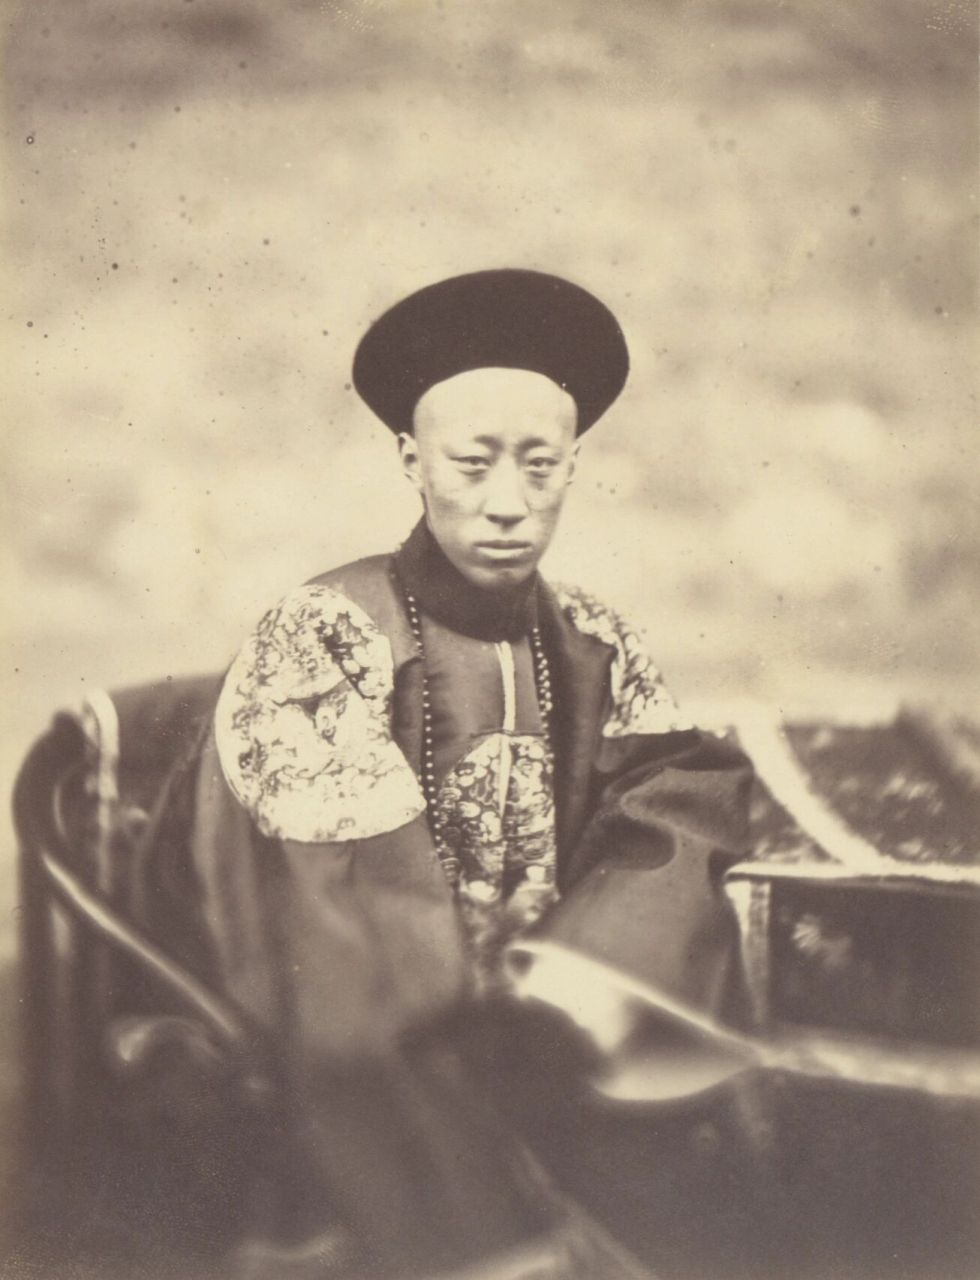
\includegraphics[width=0.7\linewidth]{Images/1}
\caption{恭亲王奕䜣(1833-1898)}
\label{fig:1}
\end{figure}

在恭亲王的支持推动下,1861年清政府通过在英国休假的海关总税务司李泰国(Horatio Nelson Lay),向英国订购了“中国”、“北京”、“江苏”等七艘西式明轮炮舰,这是近代中国迈出的通往蓝色世界的第一步(与此几乎同步,感受到太平天国军力压迫的江苏地方官员及上海本地士绅,也委托常胜军统领华尔的弟弟亨利·华尔(F.H.G.Ward)在美国购舰,分别命名“大清”、“江苏”、“浙江”,后值美国南北战争爆发,3舰被亨利·华尔擅自转售给美国北方政府,参加了南北战争)。血液里有着纳尔逊家族遗传的李泰国(李泰国的母亲是英国海军英雄纳尔逊的侄女),在英国政府默许下,将这次购舰活动看作是控制中国海上力量的机会,擅自委任英国海军上校阿思本(Sherard Osborn)为编队司令,舰队成员几乎全部雇佣英国人组成,并自作主张,单方面制订了绿底黄十字海军旗和舰队规章制度,规定舰队只服从中国皇帝和李泰国的命令,而且中国皇帝的命令必须在得到李泰国的认可后才能生效。这支全由英国人组成的中国舰队,几乎成了李泰国私人部队,史称李泰国舰队、阿思本舰队、吸血舰队等。7艘军舰远涉重洋抵达中国后,清政府对这支不受控制的舰队表现出了无论如何也不能接受的立场,经过反复争辩,最终一举将这支舰队拍卖遣散了事,由此,中国建设西式海军的第一次重要努力随着7舰的散去而破灭。

\begin{figure}[htbp]
\centering
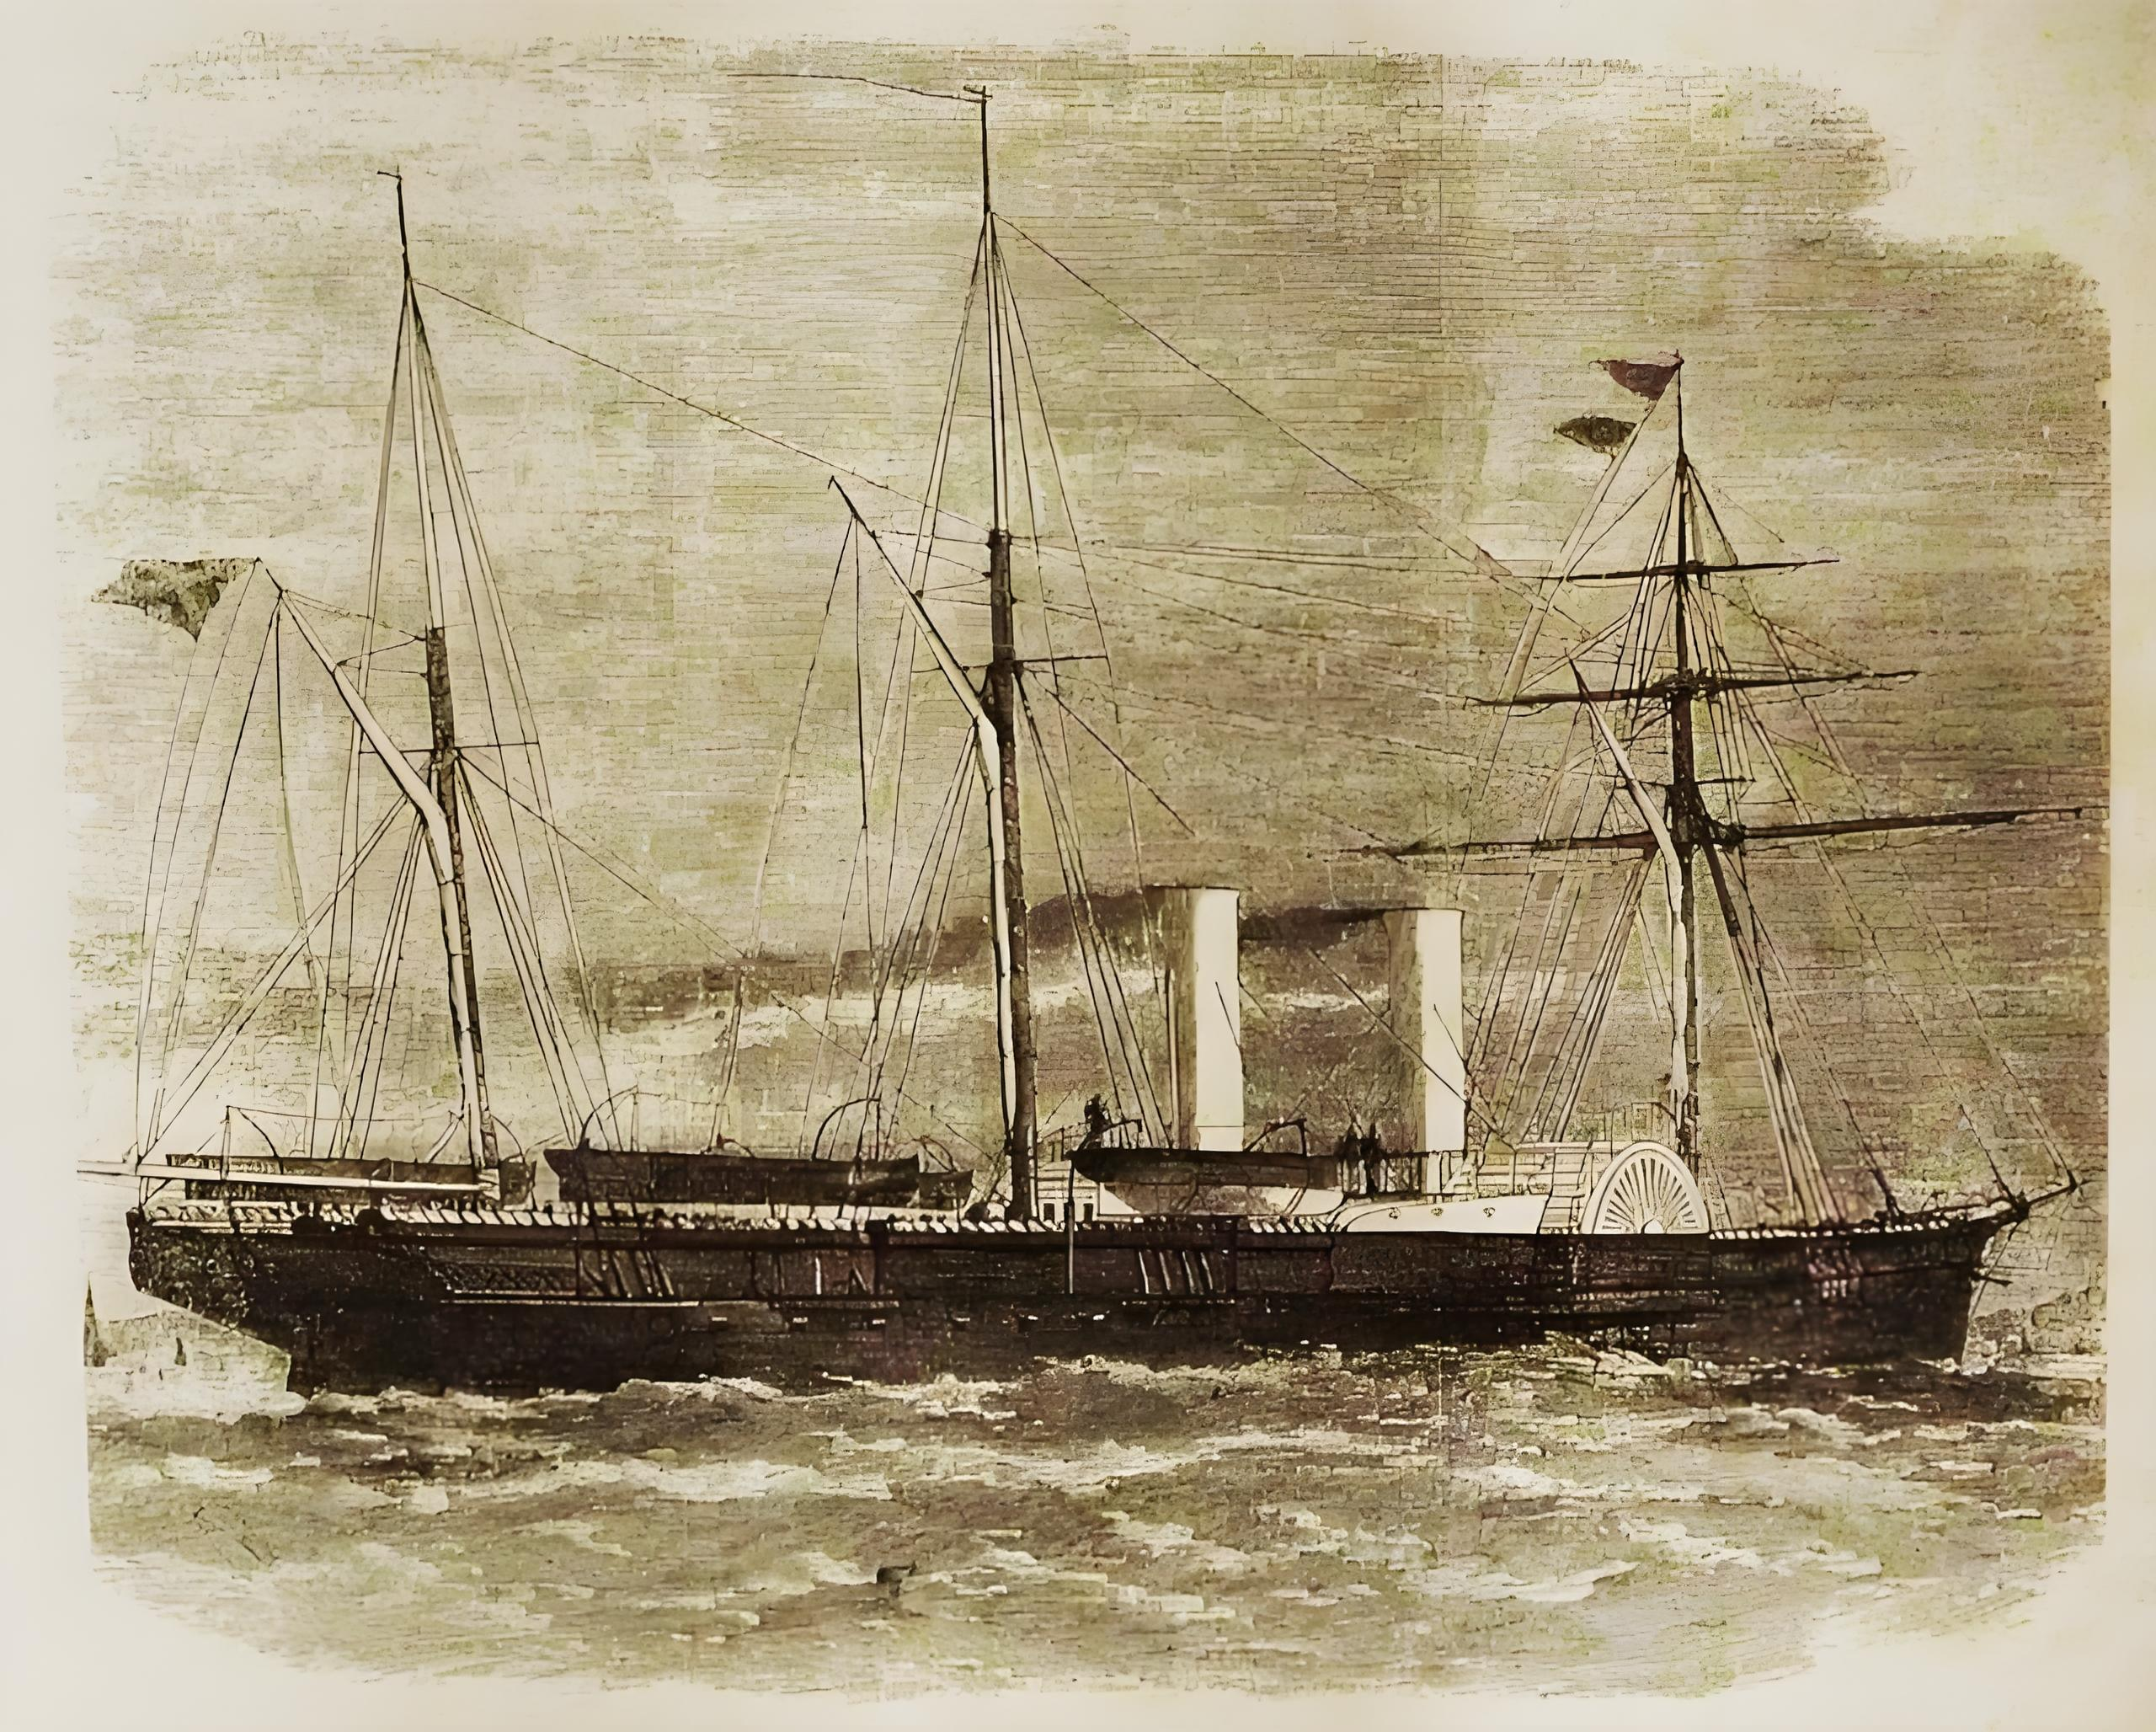
\includegraphics[width=1\linewidth]{Images/2}
\caption{西方铜版画:阿思本舰队的旗舰“江苏”号。海关总税务司李泰国组织的由英国人控制的中国舰队,给洋务官员上了教训深刻的一课,“权自我操”原则此后成为洋务活动的一条不容触碰的红线。}
\label{fig:1}
\end{figure}

令朝野上下极为难堪的阿思本舰队事件发生以后,中国国内“造舰”的呼声逐渐高涨,第一次出师就铩羽而归的教训,使得洋务派被迫更加谨慎地去对待一切与西方的交往事务,直接向西方获取军舰等武器,被认为是极易触及主权问题的敏感活动,就此很少有人愿意再涉足。此后,闽浙总督左宗棠、两江总督曾国藩先后在马尾、上海创建西式造船机构,开始了自力更生,自行建造近代化军舰的尝试。由于不可避免地受到技术起点低,专业人才匮乏,以及指导思想上存在误区等因素桎梏,这一阶段中国自行建造的军舰普遍存在舰型等级低等问题,大都属于炮舰和运输舰范畴,尚无法满足远洋作战的需求。

1871年,中国属国琉球的商船遭遇风暴漂流至福建省台湾岛,因言语不通,琉球船民与台湾土著发生争执,部分船民遭杀害。对于这一内政事件,清政府很快予以措置进行平息。但当时谁也未曾想到,与此毫无瓜葛的日本竟会借机生事。近代日本开始明治维新后,将对外扩张作为国策,为此整军经武,加强陆海军力量。1874年,借口要为琉球船民报仇,日本出兵大举入侵台湾,史称台湾事件。与此针锋相对,清王朝派船政大臣沈葆桢为钦差,赴台湾处置事变,船政水师舰船被纷纷调往,保障台湾海峡的交通、运输,以及与侵台日军抗衡、对峙。经过长时间相持,最终在列强调停下,这一事件草草收场。囿于当时海防力量薄弱,“明知彼之理曲,而苦于我之备虚……实以一经决裂,滨海沿江,处处皆应设防,各口之防难恃不得不以慎于发端\footnote{《同治十三年九月二十七日总理各国事务衙门奏》,中国近代史资料丛刊《洋务运动》1,上海:上海人民出版社1961年版,第26页。}”,担心事态扩大后无法应对,为尽早息事宁人,清王朝付出高昂的代价,除支付50万两银军费外,还被迫承认日本侵略台湾的举动是“保民义举”,实际上等于已经默认日本对中国、琉球藩属关系的挑衅,由此埋下了琉球亡国之祸的伏笔。

自三国时代以来,日本就被中国称为倭国,视为化外蛮夷,动辄对其嗤之以鼻,不以为然。然而,就是这个一贯被中华瞧不起的东邻小国,学习了一些西方先进技术后,竟然肆无忌惮向中国发起挑战,由此在中国社会引起的震动不啻于一声晴天霹雳。海防建设的重要性、紧迫性突现,而中国自造舰只存在的不足也暴露无遗。恭亲王奕䜣事后曾痛心疾首地在奏章中写道:“今日而始言备,诚病以迟;今日再不修备,则更不堪设想矣!”并追思自鸦片战争之后,中国尽管开展了建船厂、造军舰等旨在自强的事业,但“人人有自强之心,亦人人为自强之言,而迄今仍并无自强之实,从前情事几于日久相忘”\footnote{《同治十三年九月二十七日总理各国事务衙门奏》,中国近代史资料丛刊《洋务运动》1,上海:上海人民出版社1961年版,第26页。}。认为应当立刻抛开以往的成见,采取果断措施,尽快加强国家的海防实力。

“……查明一种快艇的吨位和造价,它的前甲板防护平台上要装载一门八十吨大炮,可在五百码外打穿二十英寸厚的钢板。问清最低必须吨位和优质货的最低价格。速复!询问保密!勿提中国!”\footnote{《赫致金第13号》,《中国海关密档》8,北京:中华书局1995年版,第20页。}

1874年10月23日,中日台湾事件交涉接近尾声之际,取代李泰国担任中国海关总税务司的赫德(Robert Hart),经由上海,向他在伦敦的忠实部下金登干(James Duncan Campbell)发去了上述这封电报。继夭折的阿思本舰队之后,清王朝第二次大规模外购军舰的活动渐渐拉开了帷幕,与第一次购舰活动用于镇压国内起义的目的不同,这次购舰主旨相当明确,就是巩固海防,抵御外侮。

\section{伦道尔式炮艇}

就在日本侵略台湾,中国朝野上下为之震惊、群情激愤的日子里,有个西方人的身影开始频繁地在总理衙门出没。身为英国在华利益的重要代言人,中国海关总税务司赫德敏锐地觉察到中国即将以日本为假想敌扩充海军的迹象。这位久居中国,深谙中国官场之道的英国人明白这将是影响未来中国海军事务的重要契机,良机不容错失,随即凭籍其特殊的身份,开始与总理衙门大臣恭亲王奕䜣密切接触,推销英国造军舰。自阿思本舰队事件之后,虽然左宗棠创立的船政福州马尾经历了近十年自造军舰的尝试,但日本竟然胆敢挑战中国,说明中国的海防实力并不见有多少起色,此时直接购买西方先进军舰的提议悄悄开始占据上风。

要加强海防,究竟应该以装备何种军舰为宜,围绕这一全新的命题,当时中国国内的官员大都是茫然无措,不知道从何做起。而喜欢夸夸其谈的赫德,本人实际对海军领域也只是略知皮毛,将中国人外购军舰的兴趣挑起后,赫德便急匆匆与远在伦敦的金登干商讨具体如何推销军舰。当时沈葆桢、李鸿章等中国官员从自己掌握的海军知识出发,急切想获取的是铁甲舰。但这种军舰造价过于昂贵,清政府一时无力负担,而且大型军舰对于操舰人员的专业技术知识也有极高的要求,遽难办理。很快,赫德和金登干都注意到了当时世界上一种最新潮的军舰,一种价格便宜,而且据说是大型铁甲舰天煞克星的小军舰。

\begin{figure}[htbp]
	\centering
	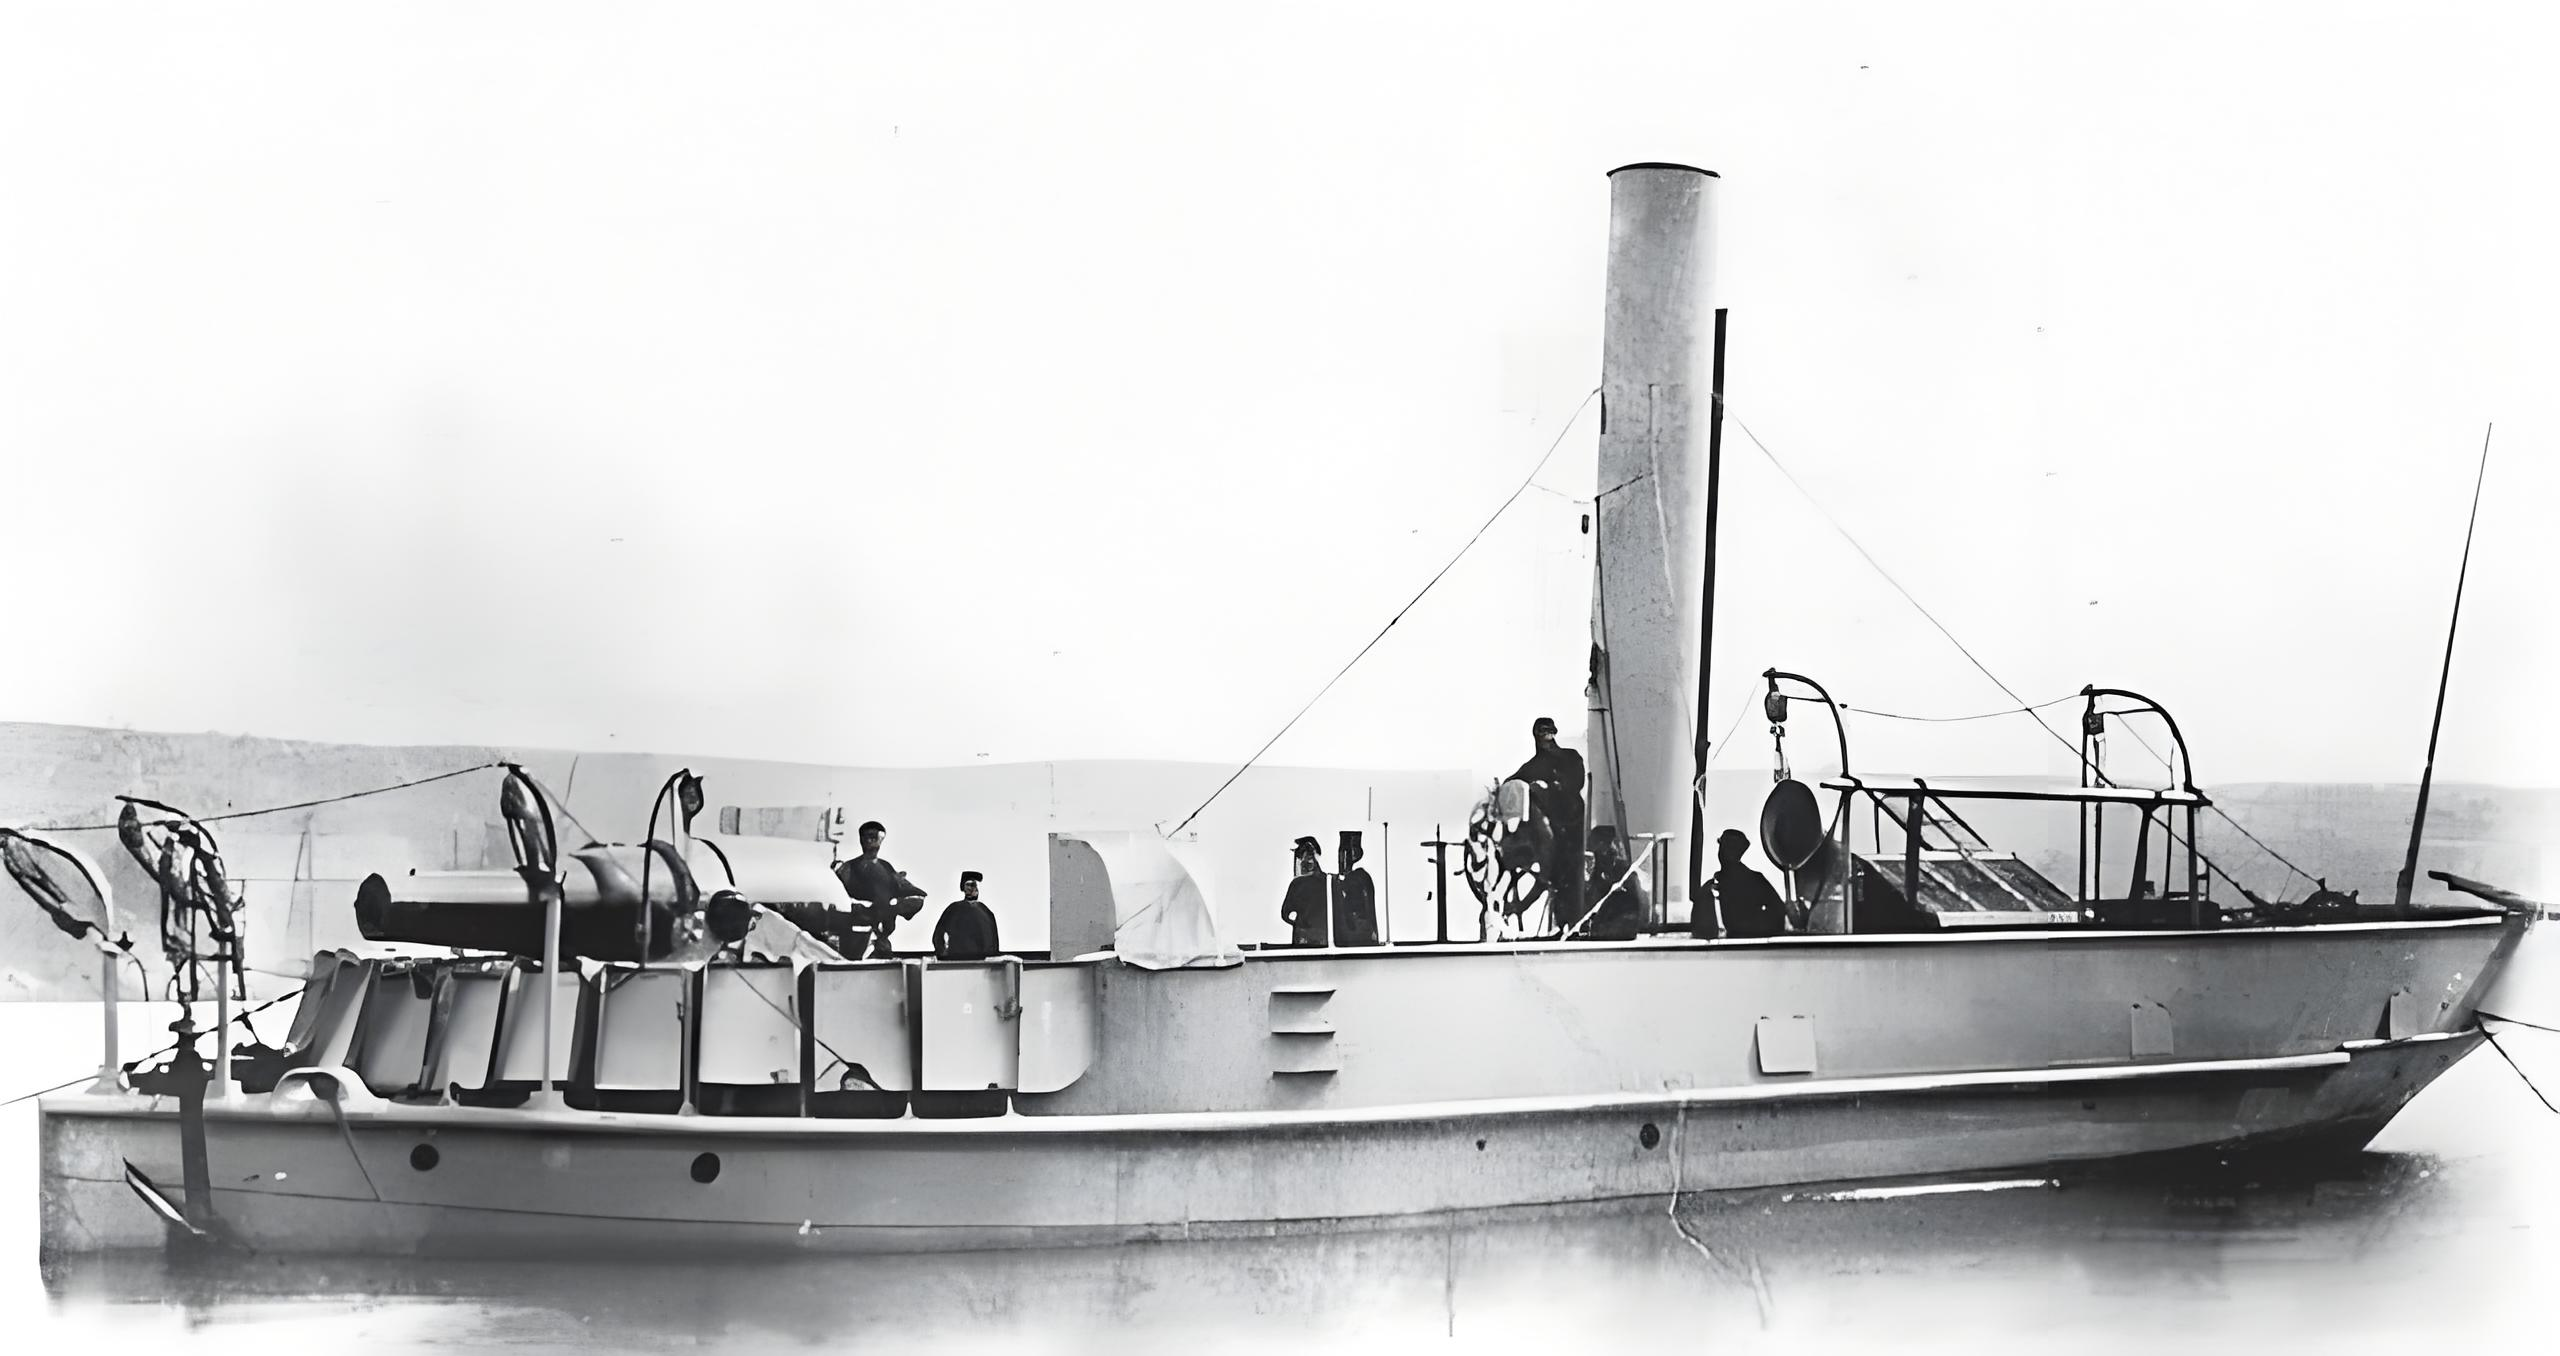
\includegraphics[width=1\linewidth]{Images/3}
	\caption{伦道尔的成名作、世界上第一艘蚊子船Staunch。依据浮动炮台的思想设计出来的这艘军舰,在当时的舰船之林中外形极为奇特,由于根本不考虑远海作战,这艘军舰完全抛弃了桅杆。}
	\label{fig:1}
\end{figure}

当中国东南马江之畔正在大兴土木建造福建船政船厂的时候,1867年12月4日,地球另一面的英国泰恩河(River Tyne)上,出现了一艘模样奇特的小军舰。在当时,连它的设计者乔治·伦道尔(George Wightwick Rendel)自己都没有想到,这艘小小的军舰竟然会成为他一生事业的重要奠基石。Staunch号,中国译为“师丹”炮船,是英国劳沃克船厂(Low Walker)建造的排水量仅有180吨的小型炮艇,长度24.38米,宽7.6米,显得短而宽,吃水1.97米,装备有2台蒸汽机、2座锅炉,主机功率150马力,航速7节。和进入蒸汽时代以来那种比巡洋舰小,航速迟缓,在甲板两侧安放火炮,“以供杂役”的旧式炮船完全不同,这艘小炮船具有几个非常鲜明的特征。它彻底抛弃了传统的船旁列炮布置法,而是在船头露天安装了一门9英寸口径的前装线膛炮,巨炮的炮身安装在一套带有4个支柱的地井式炮架上,整个系统异常复杂。平时火炮低座在船体里,以防重心过高,保持军舰的稳性,使用时则通过液压系统,在4至6分钟内将火炮举升到甲板上,每发射1发之后,火炮在自身巨大的后坐力推动下,再缓缓降到甲板下,进行下一次射击的装填工作。显得古怪的是,这种军舰在火炮发射前必须下锚,否则谁也无法预料巨大的后坐力会对小船产生怎样的影响。\footnote{Peter Brook: Warshipsfor Export-Armstrong Warships1867--1927,1999,p24.David Lyon、RifWinfield: All The Ships of The Royal Navy1815--1889,Chatham Publishing 2004,p279.Conway's All The World's Fighting Ships 1860--1905,Conway Maritime Press 1979,p111.}

除去独特的船头大炮布置方法,这艘小军舰的外形也颇具特色,舰艏有一段锚甲板,采用的是破浪效果较好的龟甲样式,上面安装有吊锚杆等设备。锚甲板向后的主甲板部分,四面都围有用于保护舰员的围壁。在船艏安装有火炮的甲板周围则装有更高的可折倒的围壁,用于防止军舰在高速航行时,海浪扑进火炮甲板。军舰的主炮炮管通过这道围壁前方一个很小的炮门开口向外伸出,因为炮门横向空隙很小,主炮几乎不能左右转动,必须采用整船瞄准法,即通过军舰的自身转动,来实现调整火炮的横向射击角度。为此,伦道尔将这艘小军舰的操舵系统设计得极为灵便,转舵速度较一般军舰为高,仅用2分45秒全船就可以旋转一圈。在接近主甲板中部的位置上,矗立着高高的烟囱,让当时的造船界为之惊讶的是,这艘小船竟然连一根桅杆都没有,而且在这艘船上除了舰长室外,甚至没有为舰员留出任何居住空间。浅眼来看,这些设计,不光是无法远距离航行,甚至连如何悬挂航海信号旗帜都成了问题。其实伦道尔赋予这种军舰独特的设计思路就在这里得到了最好的诠释。即,这种短宽的小型军舰根本就不是用来出海作战的。

\begin{figure}[htbp]
	\centering
	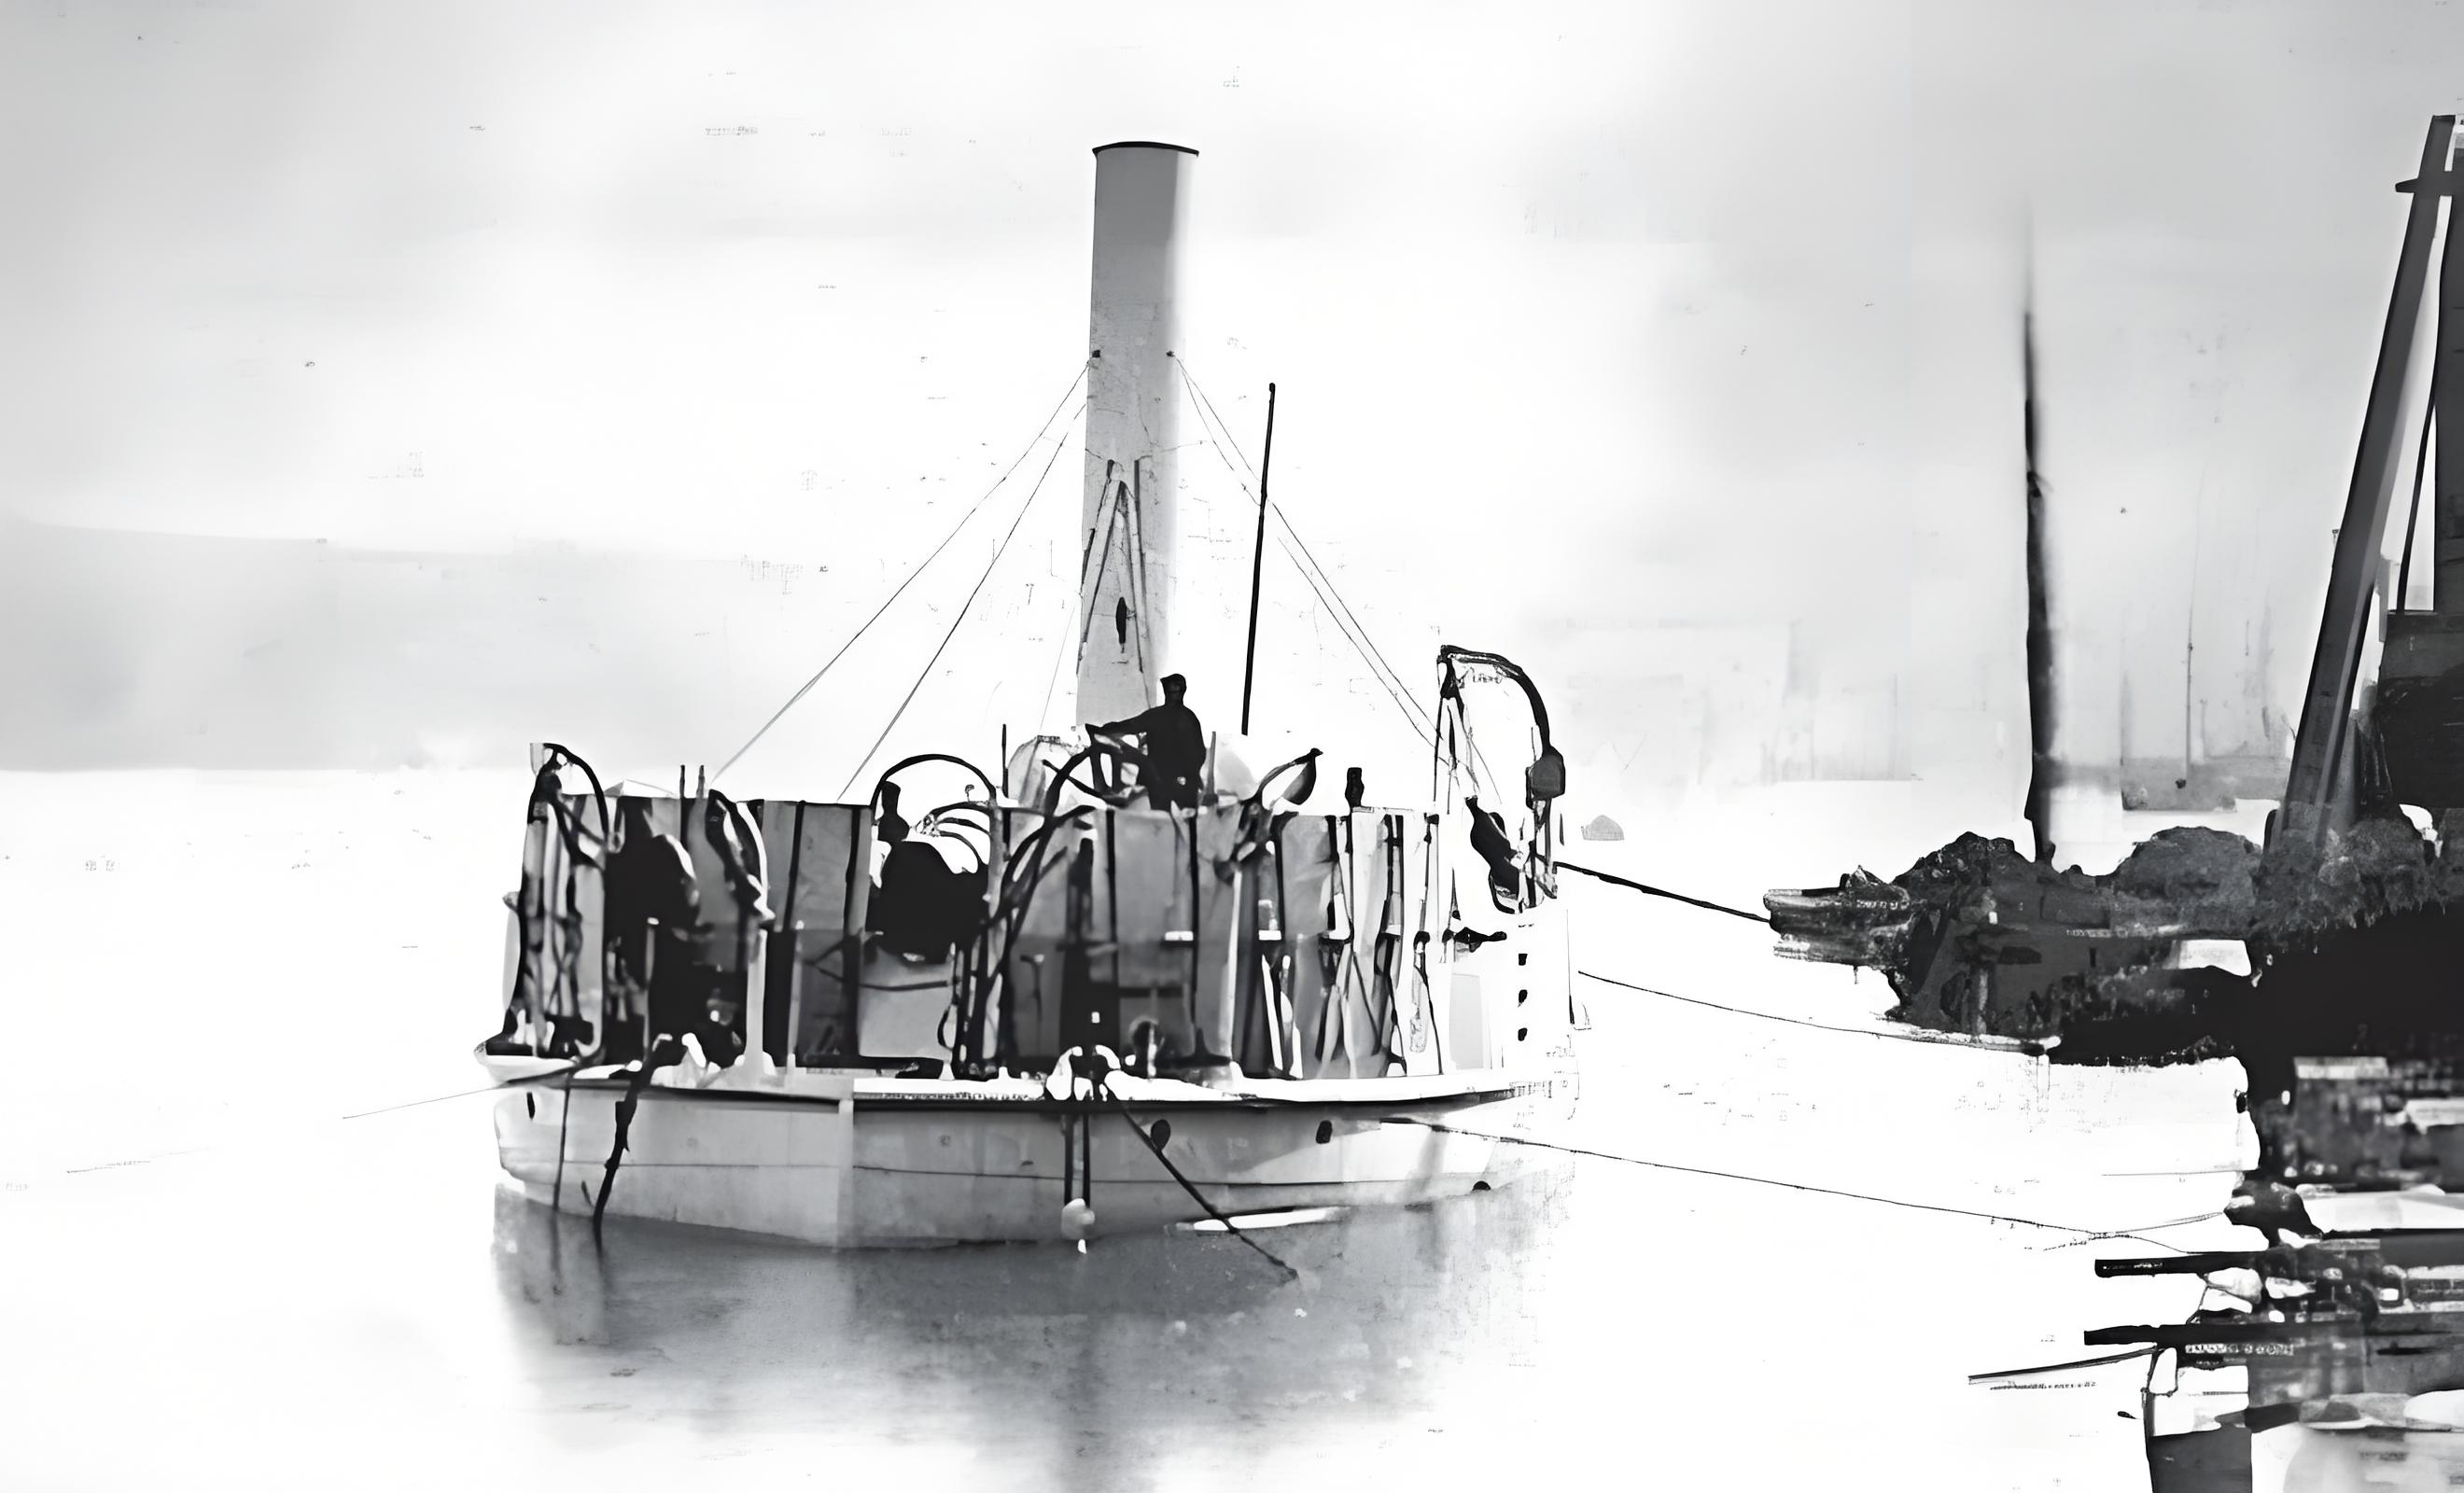
\includegraphics[width=1\linewidth]{Images/4}
	\caption{Staunch号的另一张照片,此时船艏防浪围壁是竖起状态。}
	\label{fig:1}
\end{figure}

19世纪中期的世界,大口径火炮是最具威势的兵器。在海洋上,它的搭载平台是大型铁甲舰,陆地上,则是坚固的炮台工事。结果铁甲舰和炮台发展成了一对相生相克的冤家,相对于铁甲舰,炮台上黑洞洞的巨炮阴森可怖,难以冒犯,而炮台由于是固定的建筑,万一铁甲舰不进入自己的防守范围,而是另辟蹊径,暗渡陈仓,炮台就成为虚设。为解决这一对矛盾,当时各国的陆海军界都绞尽脑汁,结果往往落入无限增大火炮口径、威力的套路中。

\begin{figure}[htbp]
	\centering
	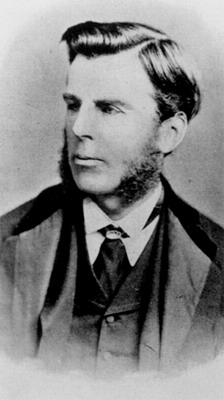
\includegraphics[width=0.5\linewidth]{Images/5}
	\caption{乔治·伦道尔,英国近代著名舰船设计师,因开创了蚊子船这一独特的舰船样式而闻名,此后他又创造了具有开创性的军舰——“超勇”级撞击巡洋舰,与近代中国海军的渊源颇深。}
	\label{fig:1}
\end{figure}

伦道尔的Staunch创造了一种全新的武器——“水炮台”,即水上的炮台,外形看上去是艘船,实则并不作为军舰来使用,搭载巨炮的小船只不过是大炮的安装平台而已。水炮台和同样装备大口径火炮的铁甲舰相比,造价上可谓有着天壤之别,但装载的火炮所具有的威力却并无太大不同,属于低成本、极具性价比的火炮搭载平台。虽然不能到大海上与铁甲舰争雄,但是它搭载的火炮同样可以给铁甲舰以巨大的威慑,近海防御时占有优势。而相对于耗费大量土木人工,经年累月才能构筑起来的陆地炮台,水炮台在价格低廉的优势之外,还有一个更大的优势,就是这种“炮台”能够移动。可以根据实际情况,临时大量布置到需要加强的濒海地域,“驻扼口隘其力能拒甲舰”,短时间内即能构成一个海上的炮台群。

这种名为炮船Gunboat,实则是炮台的军舰,在当时中国被翻译为“根驳”船、“根婆子”,又根据其特征称为“蚊子船”,意指这种军舰虽然体格小巧,不过万一被叮上一口,也不是好受的事。在西方,这种军舰则根据设计师的名字称为伦道尔式炮艇。它一经诞生,立刻引起轰动,被认为是用于要港防御的最新利器,英国皇家海军前后共购进了数十艘,其他一些海军国家也都大感兴趣,纷纷解囊采购,设计师伦道尔由此名扬四海。

1874年发给金登干的电报中,赫德所询问的“快艇”正是这种伦道尔式炮艇。赫德深知当时清王朝的财政情况捉襟见肘,与其推销短时间内中国根本没能力购买的大型铁甲舰,不如推销这种价格低廉,而且据称能打败铁甲舰的小型炮艇——蚊子船。同时,英国人并不希望中国拥有一支具有远洋作战实力的真正海军,他们所愿意看到的仅仅是中国能维持一支小规模的近海巡缉力量,能够自行绥靖海面,对付盗匪就已经足够。

今天值得重新审视的是,尽管赫德、金登干为推销军舰不遗余力,大肆宣传,但赫德对蚊子船的用途其实有清醒的认识,称这种船只是在浅水区对付铁甲舰的利器。对这一点,李鸿章也予以认同,认为“有此巨炮小船,守口最为得力,较陆地炮台更为灵活”。至于后来金登干等夸夸其谈,越说越奇,宣称这种军舰能在波涛汹涌的大海上作战,则纯属其一贯说话夸张的浮夸作风,实际李鸿章、赫德等从一开始就已经明了,这型军舰就是一种水上炮台。而后来很多对舰船知识一无所知的言官文人,以李鸿章买回来的蚊子船并不能出海作战为由,认为这种船是西方生产的劣质货,是专门设计用来诈骗中国的,则多少有些不辨菽麦的嫌疑。实际情况是,针对所谓蚊子船可以出海作战的荒谬说法,李鸿章根本不为所惑,而且在南洋大臣沈葆桢的催促下,私下已在打探丹麦、美国等国出售二手铁甲舰的信息。

1875年春天,经过向阿姆斯特朗公司询价,赫德正式将舰型方案提交给总理衙门,对这种新潮事务拿捏不稳的恭亲王则击鼓传花,将具体洽谈、购办的责任转交给北洋大臣李鸿章。从太平天国战争时代,就开始和西方人打交道,并在自己的军队中大量采用西式武器的李鸿章,是当时中国官场少有的善于处理外交事务的高层官僚,而且又身负京畿防务重责,选择他来办理新潮的海军,在恭亲王看来是再适合不过的人选。作为这一决策的继续,不久之后一道谕旨降到李鸿章面前:“著派李鸿章督办北洋海防事宜……所有分洋分任练军设局及招致海岛华人诸议,统归该大臣等择要筹办”\footnote{《光绪朝上谕档》1,桂林:广西师范大学出版社1996年版,第108页。},从此李鸿章成了中国北方海防建设的主管官员。

得到恭亲王授意,赫德奔赴北洋大臣驻地天津,上门咨商推介蚊子船。最后摆在李鸿章面前的,分别是装备80吨、38吨、26.5吨前膛火炮的三种方案。精明老道的李鸿章并没有立刻表态,而是四处咨询关于这些军舰的各种情况,并私下通过法国公使以及江海关直接获取国外市场行情,以做参照对比。咨询过程中,李鸿章突然发现一个问题:“查西人论炮不计身重,先问口径若干寸”,即按照海军专业用语,谈论火炮的类别一般都是说火炮口径而没有拿火炮的重量作为类别区分标志的,李鸿章似乎是觉察到了一点什么。\footnote{《复议购办枪炮铁船》,《李鸿章全集》31,合肥:安徽教育出版社2008年版,第140页。}赫德、金登干顿时显得颇为狼狈,急忙设法补充了相关参数。经过完善后的资料可见,当时提出的备选方案分别是:排水量1300吨,装备16英寸口径火炮,报价93000英镑,合279000两银;排水量440吨,装备12.5英寸口径火炮,报价33400英镑,合100200两银;排水量320吨,装备11英寸口径火炮,报价23000英镑,合69000两银;排水量260吨,装备9英寸口径火炮,报价20000英镑,合60000两银。\footnote{《赫总税司面译金登干来函》,《李鸿章全集》31,合肥:安徽教育出版社2008年版,第197-198页。}

经过一番权衡,李鸿章致函总理衙门,表示对恭亲王创办西式海军决心的感佩,从造价、可信度等角度出发,将备选的几家外国洋行全部否决,支持恭亲王通过赫德购买军舰的想法,认为“总税司经办当较洋行可靠”。随后,便与赫德进行仔细会商,认为备选方案中排水量260吨、装备9英寸口径火炮的型号,其火炮的威力和船只吨位都过小,意义不大。排水量1300吨,装备16英寸口径巨炮的舰型,吃水过深,且火炮口径太大,“为泰西向未有之巨炮”,担心这种从来没有使用前例的火炮不够可靠,不甘心为试验这种火炮买单,于是将这两个方案予以舍却。决定订购装备12.5英寸和11英寸口径火炮的蚊子船各1艘,旋又因各订1艘过于单薄,改为各订造2艘,同时约定,未来如得到16英寸口径巨炮使用可靠的消息,可以考虑再订购1艘装备16英寸口径火炮的大型蚊子船。\footnote{《致总署议购船炮》,《李鸿章全集》31,合肥:安徽教育出版社2008年版,第202-203页。}

4艘蚊子船由中国海关经手代办,向英国著名的火炮生产商阿姆斯特朗公司(Armstrong)订造,为预防阿思本舰队事件重演,1875年4月,李鸿章与赫德仔细订立了购舰合同,除了用大量文字就军舰的型号、质量、验收条款进行详细规定外,合同中载明,将来帮助驾驶军舰到中国的英国水手,在交接完毕后必须立刻离开中国。根据合同,装备11英寸火炮的蚊子船造价23000英镑,装备12英寸火炮的蚊子船造价33400英镑,分别折合中国银76659两和111322两,外加运费65940两,总计合同金额45万两银。按照阿姆斯特朗公司的惯例,合同签订后先付1/3,军舰造成一半后再付1/3,全成后付剩余部分。\footnote{《与赫总税司议定购办船炮章程》,《李鸿章全集》31,合肥:安徽教育出版社2008年版,第198页。}由恭亲王奏请,清政府批准合同,并对购舰经费做出布置,从江汉、九江、江海、浙海、粤海5口的海关关税内提取。\footnote{《光绪元年四月初二日总理各国事务衙门奕訢等奏折附片》,中国近代史资料丛刊《洋务运动》2,上海:上海人民出版社1961年版,第335-336页。}

1875年6月22日,赫德致电金登干,通知他中国购买4艘蚊子船的首付已经汇至专门的账户,要求立即准备合同草案、规格书、蓝图,迅速开工,“已去公文授权你从阿姆斯特朗厂购买四艘战舰,两艘载二十六吨大炮,两艘载三十八吨大炮,钱已交银行。”近代中国第二轮大规模的外购军舰活动正式开始。\footnote{《赫致金第10号》,《中国海关密档》8,北京:中华书局1995年版,第45页。}

\section{“龙骧”“虎威”;“飞霆”“策电”}

出于对自己第一次经手购舰的慎重,赫德在向金登干下达购买军舰指令的电文中,特别强调了军舰的质量。不久后,金登干便与阿姆斯特朗公司签订合同,规定11英寸口径大炮的蚊子船要在8个月内建成,装备12英寸口径炮的蚊子船限期13个月建成。\footnote{《金致赫第47号》,《中国海关密档》8,北京:中华书局1995年版,第53-54页。}4艘军舰的火炮由阿姆斯特朗公司制造,军舰的舰体部分转包给泰恩河畔纽卡斯尔(Newcastle)的米切尔船厂(Mitchell)建造。很快,4艘新潮军舰在英国的船台上陆续开工了,金登干为方便起见,用希腊文字母分别将她们命名为“阿尔法”、“贝塔”、“伽马”、“戴而塔”(Alpha、Beta、Gamma、Delta),因为这种独特的命名方式,中国蚊子船在西方又有个别号:字母炮艇。

其中“阿尔法”、“贝塔”属于装备11英寸口径火炮的一级,1875年9月21日同时开工,工厂建造编号327、328。舰体完全铁质,整体布局和蚊子船的开创之作Staunch非常相像。军舰排水量320吨,舰长35.97米,宽8.23米,吃水2.29米,动力系统为2台汤普森公司(Thompson)造蒸汽机、2台燃煤锅炉,主机功率235马力,双轴推进,航速10节,煤舱标准载煤40吨,最大载煤50吨。为保证军舰达到设计标准的机动性,军舰艏艉水下的线型完全一样,而且都安装有舵叶。\footnote{Conway's All The World's Fighting Ships 1860-1905,Conway Maritime Press 1979,p399.Peter Brook:Warships for Export-Armstrong Warships 1867-1927,1999,p30.}

这级军舰的主要武器便是安装在船头的阿姆斯特朗11英寸口径2号前膛炮,属于从炮口装填的前装线膛炮,火炮实际口径279.4毫米,炮管长4318毫米,药膛长660毫米,炮管内壁有9根来复线,每根长3023毫米,火炮可以使用3种炮弹,实心弹与开花弹均重249千克,霰弹重242千克,药包重38.5千克,在274米距离上测得能击穿326毫米厚的装甲。\footnote{《各国水师炮表·英国》,许景澄:《外国师船图表》,柏林使署光绪十二年石印版,卷十一。}火炮前方的甲板下,有一套复杂的液压弹药提升、装填装置,装填时,需将火炮的炮口低俯,以便弹药从前下方装入炮膛。此外,军舰主甲板中后部两侧还各装备有1门3英寸口径的阿姆斯特朗后膛舢板炮,另外还装备有1门作为近卫武器的格林机关炮。

\begin{figure}[htbp]
	\centering
	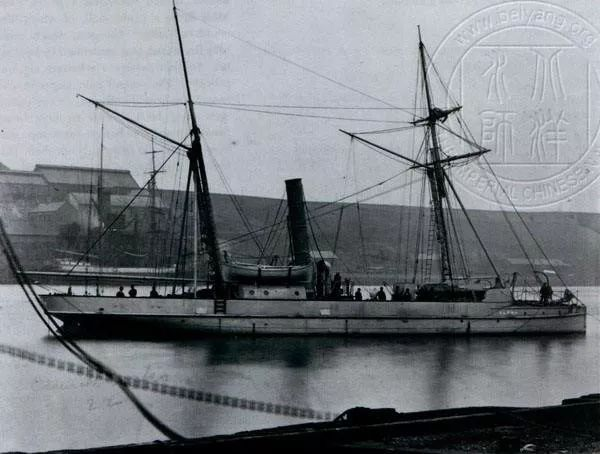
\includegraphics[width=1\linewidth]{Images/6}
	\caption{在泰恩河上进行航试的“阿尔法”(“龙骧”)舰,军舰舰艏前部的舷侧可以清楚看到临时油漆的英文舰名Alpha。和蚊子船的开山之祖Staunch外观上最明显的区别就是增加的两根桅杆。}
	\label{fig:1}
\end{figure}

相比起蚊子船的开山之作Staunch号,“阿尔法”在舰体外形上又创造了很多独特设计,考虑到这型军舰需要远涉重洋返回中国,在最初的设计上添加了2根桅杆以便挂帆,为增加强度,两根桅杆还各有人字型的副杆支撑,“阿尔法”级成了独特的带帆蚊子船。此外,“阿尔法”级主炮炮位前部外侧的装甲围壁为不能折倒的固定样式,厚度0.5英寸,具有有限的防弹片能力。在主炮之后不远,有一块对前左右三面防护,厚度同为0.5英寸的装甲挡板,作战时,指挥人员可以站在挡板之后,算是一个后部敞开式的装甲司令塔。在军舰主甲板中部的烟囱附近,设有一个位置较高视野开阔的露天指挥台,安装有舵轮、罗经、车钟等航海设备。

“伽马”、“戴而塔”是装备12英寸火炮的那级,1875年12月27日同时开工,建造编号334、335。舰体也是铁质,体形比“阿尔法”略大,排水量提升到420吨,舰长36.58米,宽9.14米,吃水2.44米,动力系统是2座汤普森公司造蒸汽机,1座燃煤锅炉,双轴推进,主机功率270马力,航速9节,煤舱正常容量50吨,最大容量60吨,军舰同样采用了艏艉舵叶。\footnote{Conway's All The World's Fighting Ships 1860-1905,Conway Maritime Press 1979,p399.Peter Brook:Warships for Export-Armstrong Warships 1867-1927,1999,p30.}主炮选用1门阿姆斯特朗12.5英寸口径1号前膛炮,也属于前装线膛炮,实际口径317.5毫米,炮身长5727毫米,药膛长699毫米,炮膛内有9根长度4330毫米的来复线,火炮同样使用3种炮弹,371千克重的实心弹、375千克重开花弹,以及373千克重霰弹,药包重72.6公斤,274米距离上测得穿甲能力414毫米,火炮的弹药提升及装填方式与“阿尔法”级相同。\footnote{许景澄,《外国师船图表》,柏林使署光绪十二年石印版,卷十一,第1-2页。}此外,“伽马”级在军舰主甲板中部还装有2门阿姆斯特朗2.75英寸口径后膛舢板炮,和1门格林机关炮。同样,考虑到回国将要经历的长距离航行,蚊子船有限的载煤难以供应,也增加了2根桅杆的全帆装设计。这级军舰从外观上整体看来,与“阿尔法”级非常相似,但是主炮周围的围壁遮护范围更大,而且主炮后方设有碉堡状的封闭式司令塔,防护方面比“阿尔法”有所改进。

\begin{figure}[htbp]
	\centering
	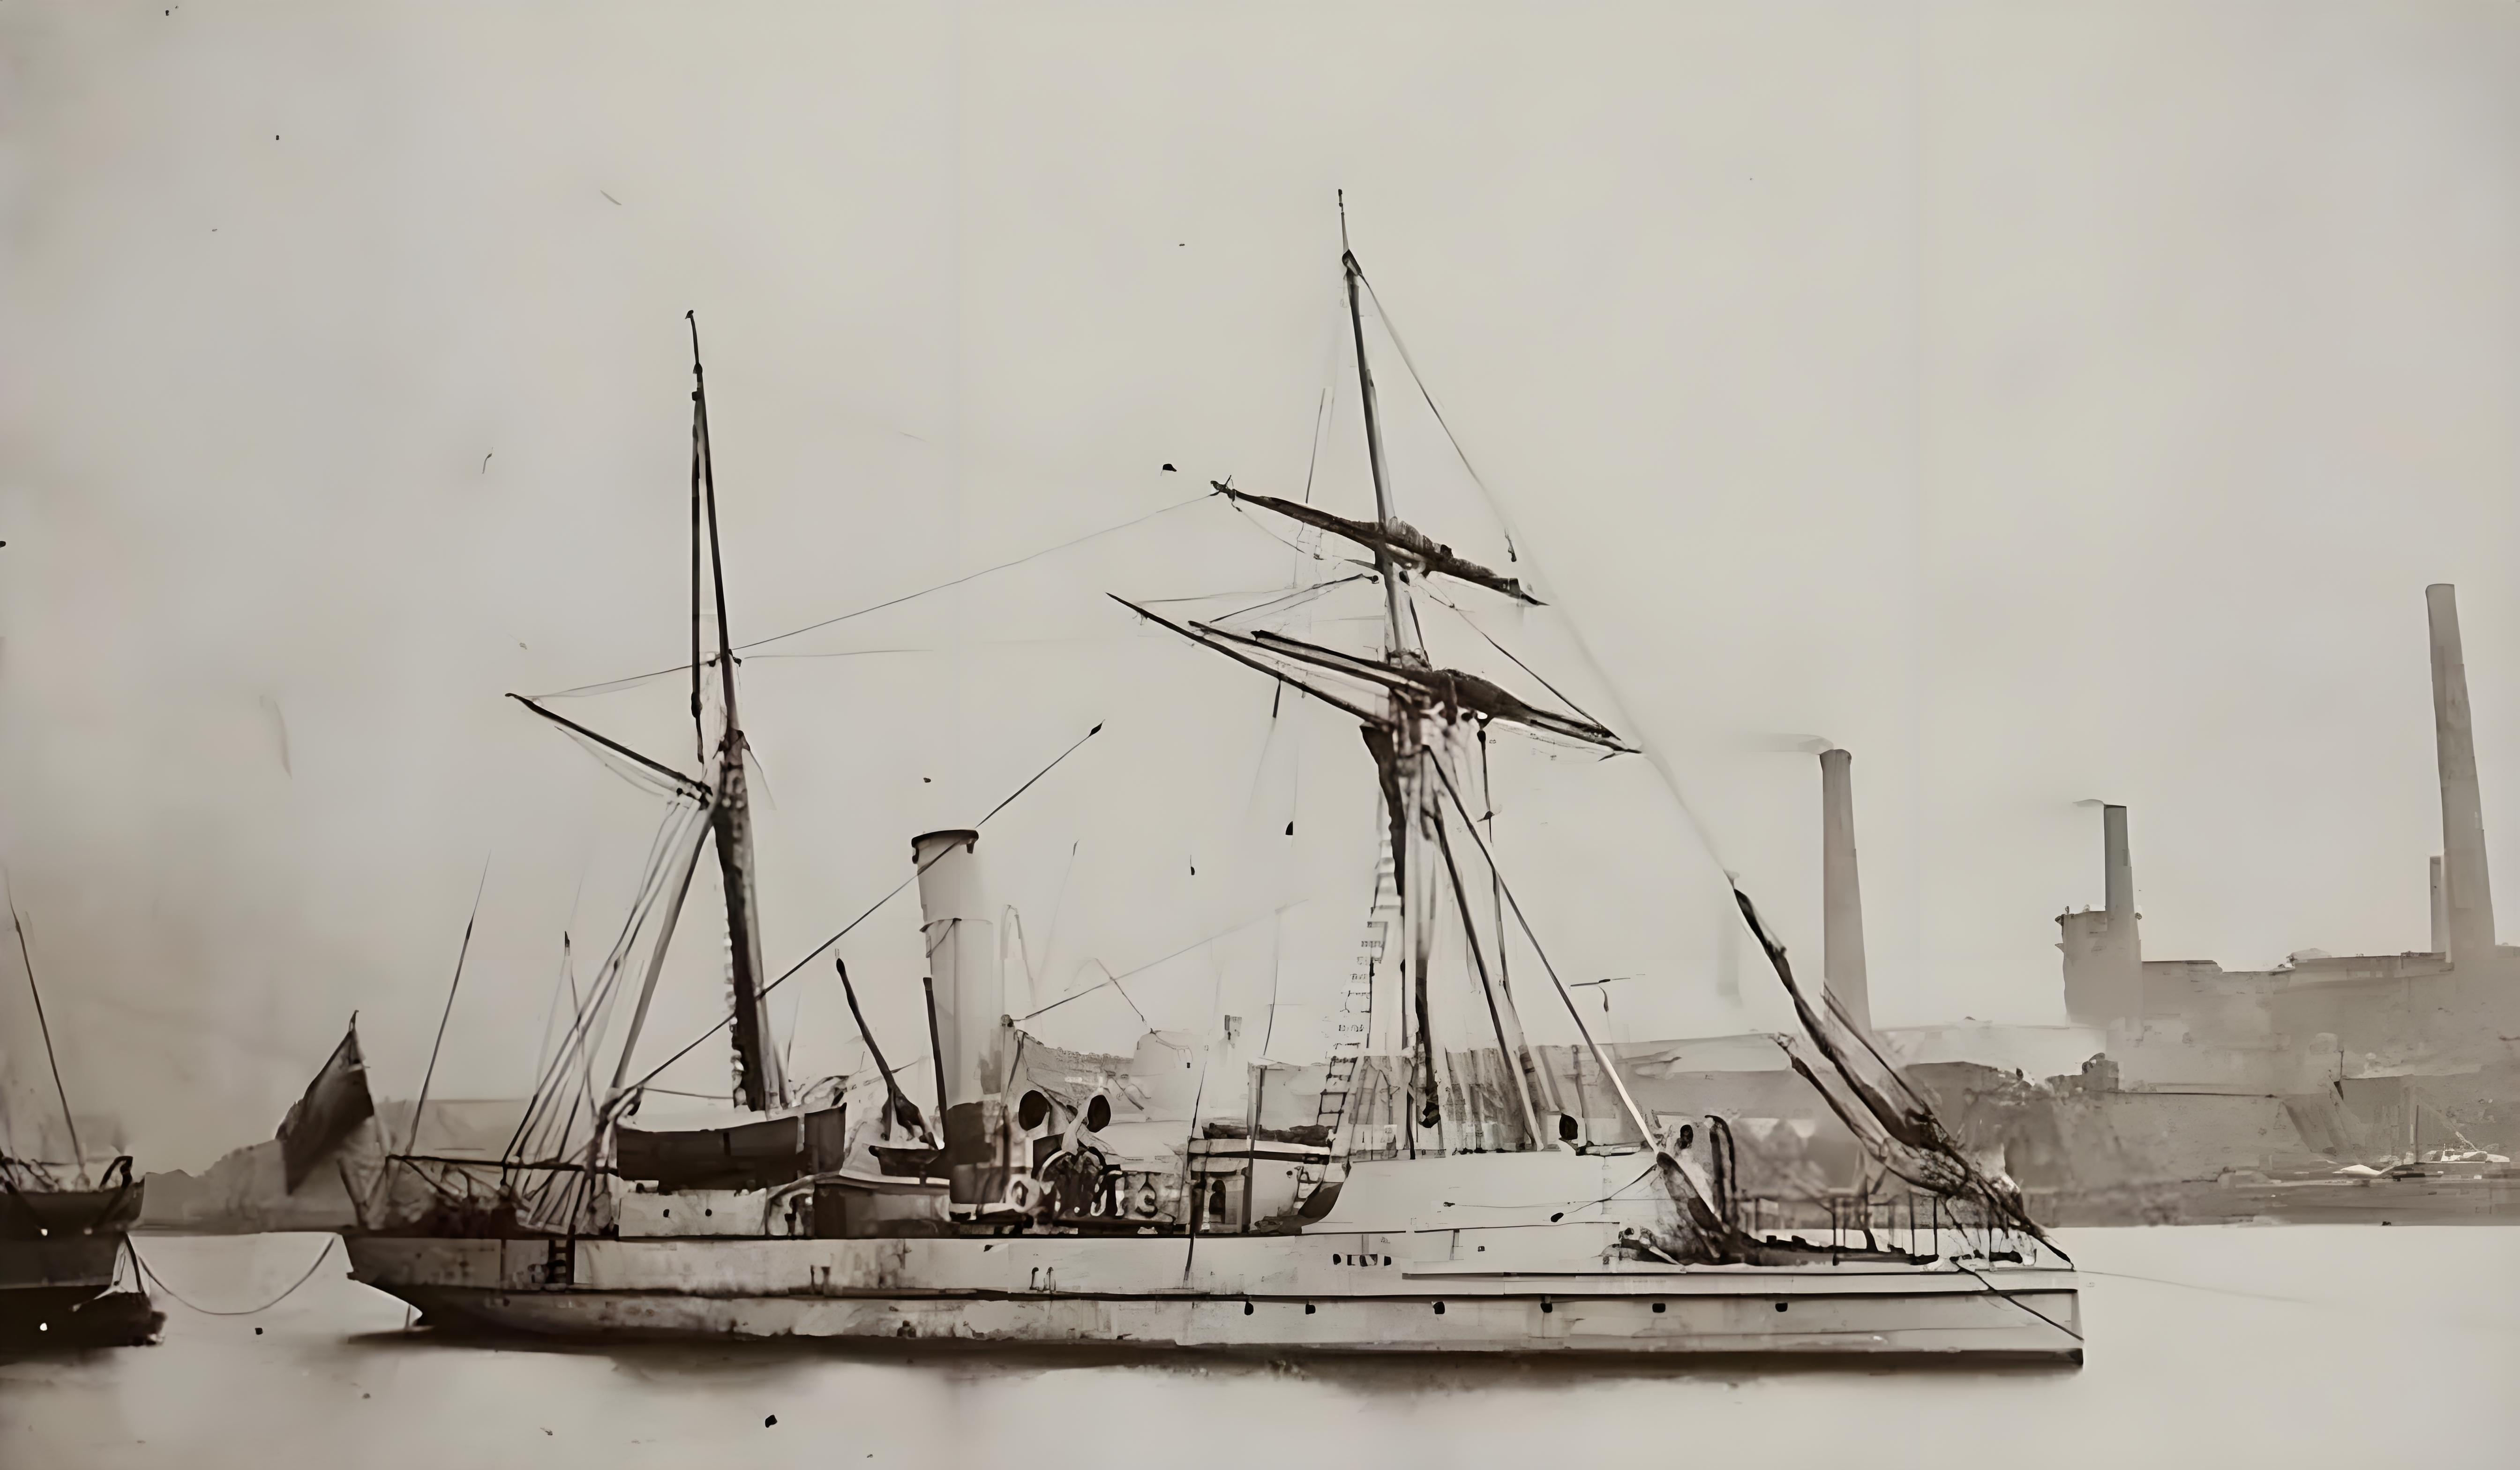
\includegraphics[width=1\linewidth]{Images/7}
	\caption{整装待发、准备回国的“戴而塔”舰,舰首舷侧的Delta舰名清晰可见,舰艉飘扬的则是英国商船旗。由于蚊子船自身煤舱容量很小,难以作远距离航行,中国的蚊子船都添加了桅杆的设计,以便必要时借助风力航行。}
	\label{fig:1}
\end{figure}

综合来看,2级新型军舰长宽比都较小,体形短粗,而且主机功率小,航速迟缓,并不适宜远航,的确只是守护海岸的水炮台而已。似乎是为了要做更进一步的诠释,“伽马”级在舰艏弹药库装满标配的50发炮弹后,如果不在舰艉加装10吨或12吨压舱物,则舰艏将要淹没在水面之下,这样的船,显然不是用于海战的。

4艘新军舰的建造过程非常顺利,“阿尔法”“贝塔”分别于1876年2月23日和4月13日顺利下水,\footnote{Peter Brook:Warships for Export-Armstrong War是平时1867-1927,1999,p30.}6月5日,金登干和英国海军部首席舰船设计师查看了2舰,表示非常满意。\footnote{《金致赫第94号》,《中国海关密档》8,北京:中华书局1995年版,第78页。}6月14日,米切尔船厂里一片热闹,意大利、丹麦等对蚊子船抱有浓厚兴趣的国家,纷纷派出武官来现场参观为中国建造的这2艘最新式蚊子船的试航,“阿尔法”“贝塔”按照英国海军部的规定,主炮用实弹和教练弹试射4次,军舰试航后航速达到9节,符合合同要求,英国海军部立刻出具证书,2艘军舰试航成功。\footnote{《金致赫第95号》,《中国海关密档》8,北京:中华书局1995年版,第78-79页。}

遵照李鸿章“每船制成两只,随时先送来中国天津口查验,不必俟全行制就一并送来”的要求,\footnote{《与赫总税司议定购办船炮章程》,《李鸿章全集》31,合肥:安徽教育出版社2008年版,第198页。}6月24日,在英国船长勒莫提·拉普利曼达吉,以及汉密尔顿指挥下,“阿尔法”、“贝塔”由雇佣的英国水手驾驶,踏上返回中国的航程。考虑到2艘仅有320吨的小船要涉渡重洋,每舰分别投了30000英镑的高额保险。\footnote{《金致赫第95号》,《中国海关密档》8,北京:中华书局1995年版,第78-80页。}

此后经过漫长的航行,虽然中途遇到风暴袭击,但一切有惊无险,于11月20日抵达天津塘沽。因为蚊子船上空间狭小,除了舰长室外,根本没有考虑水兵的居住空间,整个航程中,护送的英国水手必须在甲板上搭设帐篷露宿,艰劳程度可以想像。27日,李鸿章与赫德兴致勃勃亲往验收,李鸿章对军舰表示满意,认为“实系近时新式,堪为海口战守利器”,给予了2个极为威武的名字“龙骧”、“虎威”(Lung Hsiang,Hu Wei),并商调船政后学堂毕业生张成、邱宝仁分别管带。\footnote{《光绪二年十月二十日直隶总督李鸿章奏折附片》,中国近代史资料丛刊《洋务运动》2,上海:上海人民出版社1961年版,第345-346页。}赫德对这次的检阅情况却始终心有余悸,因为检阅过程中,出现了意外的事故,一名英国水手晕头晕脑,手中的步枪竟然走火,子弹紧贴着李鸿章的头顶飞过,当时李鸿章幸亏是坐着的,否则后果不堪设想,中国的近代史差点就将改写,这一火暴的插曲使赫德对此后的送舰活动充满了顾虑。\footnote{《中国海关密档》1,北京:中华书局1995年版,第534页。}接收之后,时值寒冬,李鸿章担心北方缺乏合适船坞设施,命令张成、邱宝仁率舰前往船政选募船员,又因为当时中日在琉球等问题上关系日益紧张,应福建巡抚丁日昌有关加强台澎防护的请求,“龙骧”、“虎威”由张成统领布置到台湾巡防。帮助驾驶2舰来华的英国船员,除每舰暂留3名技术军官充当教习外,其余均迅速遣返回国。

\begin{figure}[htbp]
	\centering
	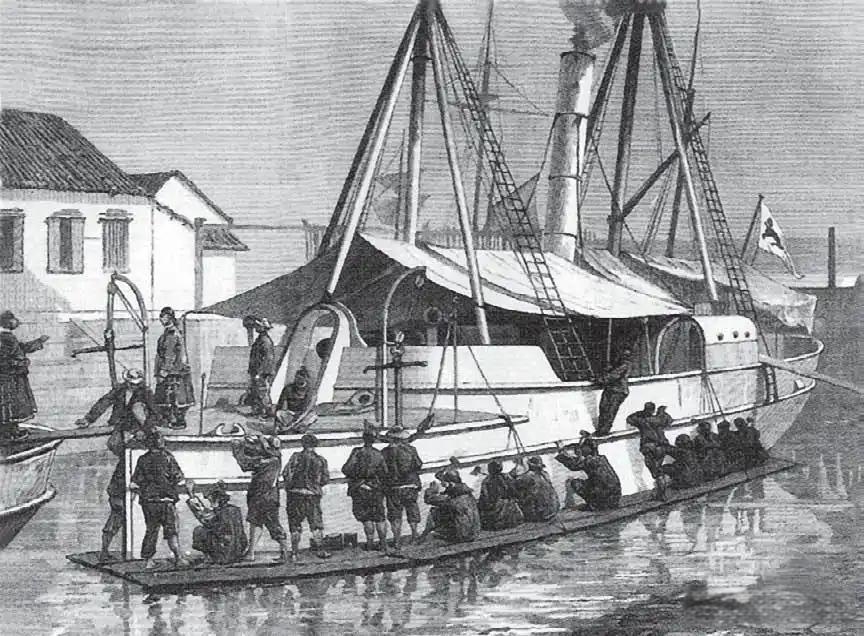
\includegraphics[width=1\linewidth]{Images/8}
	\caption{西方报纸刊登的铜版画,表现的是“阿尔法”回国后,中国工程技术人员对其进行检修、维护的情形。}
	\label{fig:1}
\end{figure}

“龙骧”、“虎威”2艘新式蚊子船整装开往遥远东方的祖国时,“伽马”、“戴而塔”在1876年6月14、23日先后下水,1877年2月17日在英国朴茨茅斯进行航试(此前在纽卡斯尔已经测得“伽马”的平均航速超过9.5节,“戴而塔”的平均航速为9节,符合设计要求。)英国海军界重要将领,以及各国驻英要员出席了试航仪式,中国驻英公使郭嵩焘亲临现场,并亲手演放了“伽马”舰的12.5英寸口径巨炮。到场参观的英国海军上将斯图尔特(Stewart),对中国的蚊子船给予高度评价:“一个真正的水兵只要一踏上船就会感到,这正是他所要的东西,是应用机械科学最渊博的知识来满足水兵的最真实的利益和需要的东西。”\footnote{《中国海关密档》1,北京:中华书局1995年版,第509页。}

第一次体验炮手工作的郭嵩焘显得非常兴奋,在当天的日记中饶有兴味地记下了蚊子船火炮系统的结构以及试炮的经过:

“初五日,金登干约至波斯莫斯观所造铁甲小船(蚊子船),安炮船首,外设炮墙护之,内复施墙,置机器。进退高低各设一机器,外推则进,内推则退,高低亦然。先推使退向内,低承前罶下(指先将炮口俯下装填弹药);而后转火药炮子以当炮口。前罶下复设机器,内推则机器直送入炮口,带水洗膛。次第送火药及炮子入,乃推置前罶下;乃复起炮使高,以度测之,而后推出炮墙外。又设电气线于机器墙内,引手按之,而声发子出,可及七千五百余步。但得一人,运机器有余,可云神妙……其‘代拉塔’(戴而塔)船亦开出海口,各演炮三,内演试群子一,船旁小炮及连环子炮皆历试之,亦平生之创见矣……”\footnote{郭嵩焘:《伦敦与巴黎日记》,长沙:岳麓书社1984年版,第117页。}

赫德担心送舰交货时再出现类似枪支走火的事故,反复叮嘱金登干加以注意,金登干起初想转嫁责任,准备干脆让阿姆斯特朗公司派人送船,最后则设法与皇家海军磋商,在确认运送的船只是最先进的军舰后,皇家海军破例批准可以让现役军官以请假的形式接受雇佣。两名现役军官琅威理(William M Lang)、劳伦斯·庆随后就被雇佣来管理驾驶“伽马”、“戴而塔”送往中国。

有现役英国军官驾驶运送,按理因当万无一失,金登干于是向赫德打包票:“您看吧!这些炮艇移交时准能像英国战舰那样——秩序井然,水手严守岗位。我认为,如果李鸿章不看一看炮艇上的英国水手是怎样操纵大炮的,那真是太可惜了……精心选拔的船员,将可充分利用这次出航的机会,来熟习和发挥这些舰只的性能。我毫不怀疑“伽马”和“戴而塔”号炮艇将以最漂亮的军舰的姿态驶抵中国。因此到达那里以后,要使各个有关方面都感到满意,这些炮艇应该受到李鸿章本人的正式视察,以使他了解到,在称职的人手操作下,这些炮艇可以达到多么高的效能。”\footnote{《中国海关密档》1,北京:中华书局1995年版,第503页。}

2月28日傍晚6点半,盘旋在英伦的恶劣天气稍稍平息,皓月当空,“伽马”、“戴而塔”鱼贯驶入英吉利海峡,踏上回国的航程。有趣的是,当时的中国公文将送舰的两位英国军官的名字分别音译为浪为美、静乐林,取风平浪静的吉祥之意,\footnote{《复福建船政吴春帆京卿》,《李鸿章全集》32,合肥:安徽教育出版社2008年版,第22页。}其中浪为美——琅威理尤其受到郭嵩焘的好评。站在飞桥上指挥若定的琅威理,脑海里可能还在想着热恋中的女友,但从这次航程开始,这个英国人与中国的海军建设结下了深深的缘分。

尽管从“伽马”、“戴而塔”出发开始,金登干就不厌其烦地向赫德介绍护送蚊子船的英国海军军官之可靠,介绍每个人的才干,甚至还把琅威理电报发回的航行日志转发给赫德。然而赫德仍然感觉不放心,要求2艘蚊子船不用直驶大沽,先前往福建船政,等自己查看后再作决断。

6月18日,“伽马”、“戴而塔”顺利到达了位于福州马尾的船政,赫德发现“它们在到达时,还不如‘阿尔法’、‘贝塔’号驶抵天津时干净、整洁”,于是决定就在福州就地交付给中国,以免去天津旁生枝节。“经过同船员们谈话,并注意看了水手们的外貌,我决定不让他们去天津,它们决不会给李留下什么特殊的印象。”\footnote{《中国海关密档》1,北京:中华书局1995年版,第561页。}6月25日,2艘蚊子船直接在船政移交中国,随即被李鸿章分别命名为“飞霆”、“策电”(Fei Ting、Tse Tien),连同先到的“龙骧”、“虎威”被重新分派军官,由从船政借调的军官邓世昌、李和、邱宝仁、吴梦良分别管带,就近在福州一带募集船员。\footnote{《复吴春帆京卿》,《李鸿章全集》32,合肥:安徽教育出版社2008年版,第40页。}

\section{蚊子船热}

“龙骧”等4艘新式军舰成功回国,立刻在中国国内引起轰动,对这种据说能够打败铁甲舰的海防利器,沿海各省纷纷表示羡慕。实际在作为国家行为的北洋购买蚊子船之前,中国沿海很多地方早已经有了购造蚊子船的活动。1875年,福建善后局就曾通过上海载生洋行向英国莱尔德公司(Cammell Laird)订购了2艘蚊子船,分别命名“福胜”、“建胜”(Fu Sheng、Chen Sheng),首开中国购买蚊子船的先河。这两艘后来移交福建船政的蚊子船,排水量256吨,长26.52米,宽7.92米,吃水2.51米,小于“阿尔法”级,主机功率180匹马力,航速8节,装备1门10英寸口径瓦瓦苏尔(Vavasseur)前膛火炮。\footnote{Richard N J Wright,The Chinese Steam Navy 1862--1945,Chatham Publishing 2000,p42;Conway's All The World's Fighting Ships 1860--1905,Conway Maritime Press 1979,p398.}而看到北洋新购的“龙骧”、“虎威”等新式蚊子船,福建巡抚丁日昌认为性能胜过“福胜”、“建胜”,主张立刻按照北洋购买的样式,为福建海防增购一批。

\begin{figure}[htbp]
	\centering
	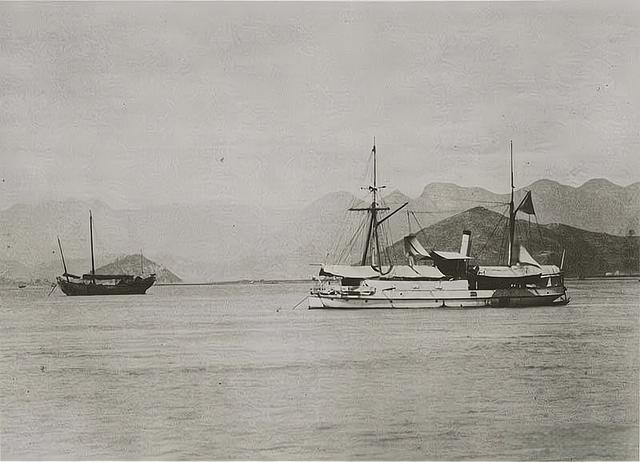
\includegraphics[width=1\linewidth]{Images/9}
	\caption{1884年中法马江之战前,停泊在马江江面的“福胜”级蚊子船。}
	\label{fig:1}
\end{figure}

与福建几乎同时,南洋治下的江南机器制造总局于1875年9月15日下水了一艘自造的蚊子船。这艘名为“金瓯”(TiongSing),寓意江山永固的军舰,诞生得极为突兀,可以看作是当时中国的军工技术人员紧密关注世界舰船发展潮流的结果。军舰排水量较小,仅有195吨(另有排水量200吨的记载),舰长31.7米,宽6.2米,吃水2.06米,主机功率304匹马力,航速10节,装备170毫米口径克虏伯后膛大炮1门。\footnote{Richard N J Wright,The Chinese Steam Navy 1862--1945,Chatham Publishing 2000,p36;Conway's All The World's Fighting Ships 1860--1905,Conway Maritime Press 1979,p398.}粗眼看来,这艘军舰除了采用后膛火炮,在当时各种蚊子船中略显时髦外,其他各项指标并不突出,似乎是泛泛之作。然而,“金瓯”实际是世界上第一艘装甲蚊子船(或称近海防御铁甲舰),中国的工厂技术人员们在这艘蚊子船上,率先引用了水线带装甲的设计,军舰沿水线装有厚2又3/4英寸的装甲,这一创举,比欧洲第一艘装甲蚊子船德国的Wespe要早。军舰主甲板上设置了一个带有2又3/8英寸厚装甲的炮塔,炮塔内还参照了西方地井炮的设计思路,通过液压装置,装填时将火炮降到舱内,装填完毕后则举升到炮台内,极为灵便。此外,“金瓯”舰在船艏还安装有撞角,“船头有铁杆一支,直伸出船外,如犀之独角”,\footnote{《申报》,1875年1月1日。}这又是蚊子船发展史上的一项创举。这艘外形不起眼,但实际运用了大大领先世界设计思想的军舰,简直可以视作是新技术的试验平台,诞生伊始就引起了西方世界的震惊,认为“灿烂可观”,而且很有可能的是,德国Wespe军舰设计之初的灵感,就来自于中国的“金瓯”,如果这一点能得到确认,那么“金瓯”将是包括“经远”在内的德系装甲巡洋舰的共同始祖。但是,这艘造价仅为62586.93两白银的军舰可能因为体量太小,并未引起中国国内过多的关注,当北洋的蚊子船回国后,南洋大臣沈葆桢即写信给李鸿章,请求能分拨1、2艘西方建造的蚊子船。

最后,甚至连英国人都来凑热闹了。1878年5月24日中午,天津英国领事馆内空气异常凝重,应英国人之邀前来赴宴的李鸿章,发现领事馆餐厅里仅有领事和3名英国海军军官而已。受克里米亚战争影响,英国担心俄罗斯借地利之便,到中国海域来攻击英国船只,为了加强在远东的海军力量,与李鸿章商谈,希望能将“龙骧”、“飞霆”级军舰全部购回,加入皇家海军防守香港、新加坡。考虑到中国海防建设刚刚起步,而且这4艘蚊子船自用尚且不够,李鸿章予以一口回绝。由此也可以看出,蚊子船这种船型,在当时各国海军中,仍属于利器一类。英国领事曾坦率地说“此式炮船……专防本国海口以作水炮台抵御铁甲,最为得力。”\footnote{《论英使密购回蚊船》,《李鸿章全集》32,合肥:安徽教育出版社2008年版,第304页。}

由4艘新型蚊子船回国,一时间,从南到北,中国沿海兴起了一股沸沸扬扬的蚊子船热。

鉴于各省纷纷要求购买蚊子船的情况,总理衙门致信李鸿章,称“此项船只,无论各海口,难资分布,即咽喉要区,根本重地尚不足数,必应即时添置”,要求李鸿章负责具体经办,尽快再增加购买一批蚊子船。当时,赫德已经返回阔别12年的家乡英国休假,顺道帮助具体操办中国参加巴黎世博会一事,李鸿章于是通过赫德在中国的内弟,海关总理文案税务司裴式楷(Mattbew Boyd Bredon)致电金登干,打听蚊子船的报价是否有变化。1878年7月8日上午,金登干收到了裴式楷由上海发来的电报:“目前情况下,‘阿尔法’或‘伽马’级炮艇实价几何,25163(暗号,可能代指李鸿章)询问,或许将订购四艘。”\footnote{《中国海关密档》2,北京:中华书局1995年版,第44页。}

经过和阿姆斯特朗公司的谈判杀价,7月28日,赫德、金登干提交了蚊子船的报价:年内购买2艘“阿尔法”级,单价26150英镑,如果购买4艘,则便宜至25500英镑。“伽马”级购买2艘,单价33300英镑,购买4艘,单价为32500英镑。\footnote{《中国海关密档》2,北京:中华书局1995年版,第63页。}考虑到吨位和火炮口径,李鸿章未再考虑小型的“阿尔法”级,决策再购买4艘“伽马”级蚊子船,总价45万两银。1878年8月29日下午,金登干与阿姆斯特朗公司签订合同,费尽口舌后,阿姆斯特朗坚持报价不能减少一分,但可以稍做让步,答应为每艘船免费加装1门格林炮(Gatling Gun)作为赠品。\footnote{《中国海关密档》2,北京:中华书局1995年版,第100页。}

\section{“镇”字号蚊子船}

中国新订造的这批蚊子船,按照他们的4艘姐姐的传统,被金登干继续用希腊文字母暂时命名,分别为“埃普西隆”、“基塔”、“爱塔”、“西塔”(Epsilon、Zeta、Eta、Theta),工厂建造编号374、375、376、377。\footnote{Peter Brook: Warships for Export-Armstrong Warships 1867--1927,1999,p30.}由于这几艘船的设计较之最初的“伽马”级做出了大量调整、改进,因而自成“埃普西隆”级。

与母型“伽马”相比,“埃普西隆”舰体的材质改成了更坚硬的钢,外观尺寸等数据也都发生了一定变化。这级军舰排水量增加到490吨,长38.1米(全长3.7米),宽8.84米,吃水2.9米,动力系统采用2台英国霍恩索公司(R\&W Hawthorn)生产的蒸汽机,配套2台燃煤锅炉,功率472马力,双轴推进,航速10.2节,采用艏艉双舵叶。煤舱容量和“伽马”相同,正常载量50吨,最大载量60吨。\footnote{Conway's All The World's Fighting Ships 1860-1905,Conway Maritime Press 1979,p399.Peter Brook:Warships for Export-Armstrong Warships 1867-1927,1999,p31.}

军舰的武备上变动较大,“埃普西隆”放弃了“伽马”级装备的12.5英寸口径火炮,改成一门口径略小的11英寸口径阿姆斯特朗火炮。担心中国人可能一时无法理解和接受这种改变,赫德、金登干和阿姆斯特朗公司提交了详尽的备忘录进行解释,称火炮的口径虽然变小了,但由于结构的改进和发射药量的加大,火力远较老式的大口径炮猛烈有力,“中国人可能认为,炮弹越大,造成的损害也会越大。然而,炮弹所造成的损害的大小,取决于推进炮弹的火药量的多少”,\footnote{《中国海关密档》2,北京:中华书局1995年版,第122页。}而且,阿姆斯特朗提出,新式火炮的重量较老式火炮轻,省出来的重量,可以用于改进设计,进一步增加军舰的航速。对此半信半疑的李鸿章最终接受了这个改变。

\begin{figure}[htbp]
	\centering
	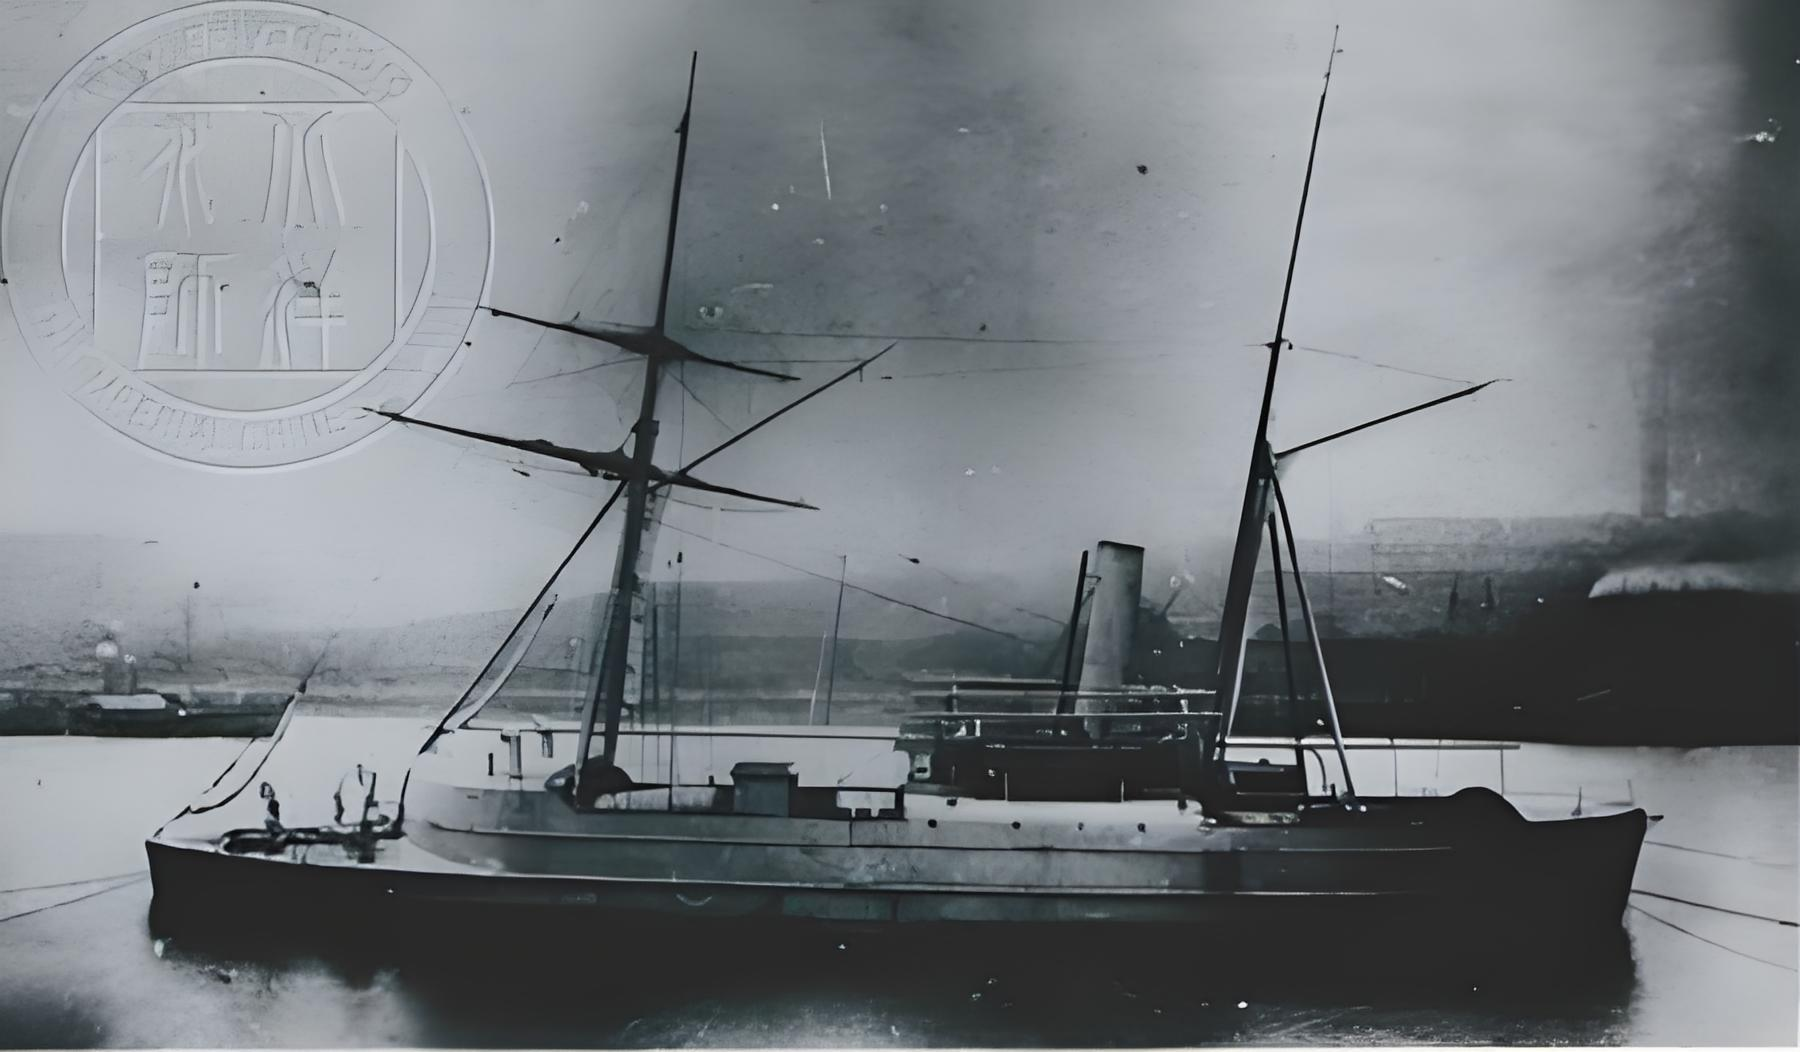
\includegraphics[width=1\linewidth]{Images/10}
	\caption{停泊在泰恩河上的“埃普西隆”“镇东”,军舰中部的飞桥上搭建了用于铺设天幕的支架。}
	\label{fig:1}
\end{figure}

新安装的11英寸口径阿姆斯特朗前装线膛火炮,实际口径279.4毫米,膛长6480毫米,弹重240.4公斤,炮重35吨,火炮初速554米/秒,射程7681米,火炮的操作以及弹药装填方式与“伽马”级相同,“大炮装在前面,用水力运转、装弹、制驭,开炮只需要5个人。瞄准时大炮的旋转并没有机械的自动设备,而是由船本身去完成回转任务……因为船身短,又装有两具推进机,所以这只小船能够依情况的需要迅速准确地旋转”\footnote{《“田凫”号航行记》,中国近代史资料丛刊《洋务运动》8, 上海: 上海人民出版社1961年版,第416页。}。此外,和“阿尔法”、“伽马”一样,主甲板上还安装有2门3英寸口径后膛炮,同样由阿姆斯特朗公司制造,实际口径76.2毫米,炮身长1920毫米,初速357米/秒,射程5800米。根据“阿尔法”、“伽马”的原先设计,军舰上还配有1门格林机关炮,因为阿姆斯特朗公司又附赠了1门,格林炮总数增加为2门。

拥有大量造舰经验的米切尔船厂,对建造这几艘小型军舰可谓驾轻就熟,建造过程一切顺利,“埃普西隆”级4艘军舰在1878年9月9日同时开工,分别于1879年1月20日、3月22日、2月5日、3月27日下水。\footnote{Peter Brook: Warships for Export-Armstrong Warships 1867--1927,1999,p30.}1879年3月25日,顾不上患病不起的妻子,金登干和曾经驾驶护送“伽马”舰前往中国的海军军官琅威理一起来到纽卡斯尔,视察了接近完工的首舰“埃普西隆”。结合在以往驾驶“伽马”远航中的切身感受,琅威理认真地对新蚊子船提出了很多修改建议,经过很长时间的辩论,伦道尔、阿姆斯特朗被说服,同意对新军舰进行某些修改。“埃普西隆”级蚊子船原本外形上和母型“伽马”非常相像,而经过这次修改后,外形上就产生了极为明显的区别。琅威理对“埃普西隆”的主要修改建议有:在主炮防护围壁上方水平敷设一块薄钢板和防波板,以便使得任何时候火炮都处于遮蔽中;将军舰的舷墙全部增高2英尺,既可以在航行时防浪,也能在战时对水手起到保护作用;将原本露天的军舰舰艉甲板,用硬质的顶棚遮护,可以免除在倒车航行时甲板上浪。\footnote{《中国海关密档》2,北京:中华书局1995年版,第182页。}经过这系列改装,“埃普西隆”的设计更加完善,成为蚊子船发展过程中的一型成熟之作。

1879年7月24日,继郭嵩焘之后出任驻英公使的曾纪泽由金登干陪同抵达朴次茅斯,一行人等分乘4艘蚊子船出海演试。在“埃普西隆”甲板下并不宽敞的餐厅内用过午饭后,曾纪泽亲手燃放舰艏的大炮,显然开炮这种带有亲身体验性质的活动很受中国官员欢迎,“炮之进退高下以及装药盛子,皆以汽机运之,启闭其机极为灵便,不过用斤许力耳。第一炮装药、盛子、进炮,皆余自启其机。”跟随在“埃普西隆”之后的“基塔”等船也各试炮2响,其中鸣响“基塔”舰大炮的是金登干的夫人,此举似乎是进一步说明蚊子船火炮系统设计之巧妙灵便。试炮完毕后,各舰又测试机动性能,360度旋回三圈,第一圈单纯靠螺旋桨,第二圈依靠舰艏舵叶,第三圈则是舰艉的舵叶,在方圆30丈的区域内,测得旋转一次平均时间为3分5秒,一切表现令人满意。\footnote{《曾纪泽集》,长沙:岳麓书社2005年版,第356页。}

7月30日,由琅威理率领,4艘“埃普西隆”级蚊子船起航回国,此前鉴于福政于1877年派出的赴欧洲海军留学生已经留学有日,为造就人才,李鸿章曾和留学生监督李凤苞协商,意图从留学生中挑选资质优良者驾驶这批蚊子船回国,不假手于西方人,然而金登干以中国学生学业未精等借口婉拒,最终仍雇用英国船员驾驶护送。

新蚊子船离开英国的当天,《泰晤士报》做出长文报道,认为这些军舰装备的火炮威力惊人,超过当时英国所有舰上火炮,表示出了对这型新式蚊子船的艳羡:“星期三清晨,在岬头(Spithead)出现了一队样式新颖的炮舰,朴次茅斯的海军界为之惊愕……它们虽然悬挂英国海军的红色旗帜,但显然不属于英国。它们是埃尔思威克工场、阿姆斯特朗公司为中国政府所建造的……中国人作此突然的冒险一跳,已经跳到我们前面去了。当人们记住这些的时候,便知道这个新创事件的重要性和所表现的勇气是值得注意了”\footnote{《“田凫”号航行记》,中国近代史资料丛刊《洋务运动》8, 上海: 上海人民出版社1961年版,第412-413页。}。

\begin{figure}[htbp]
	\centering
	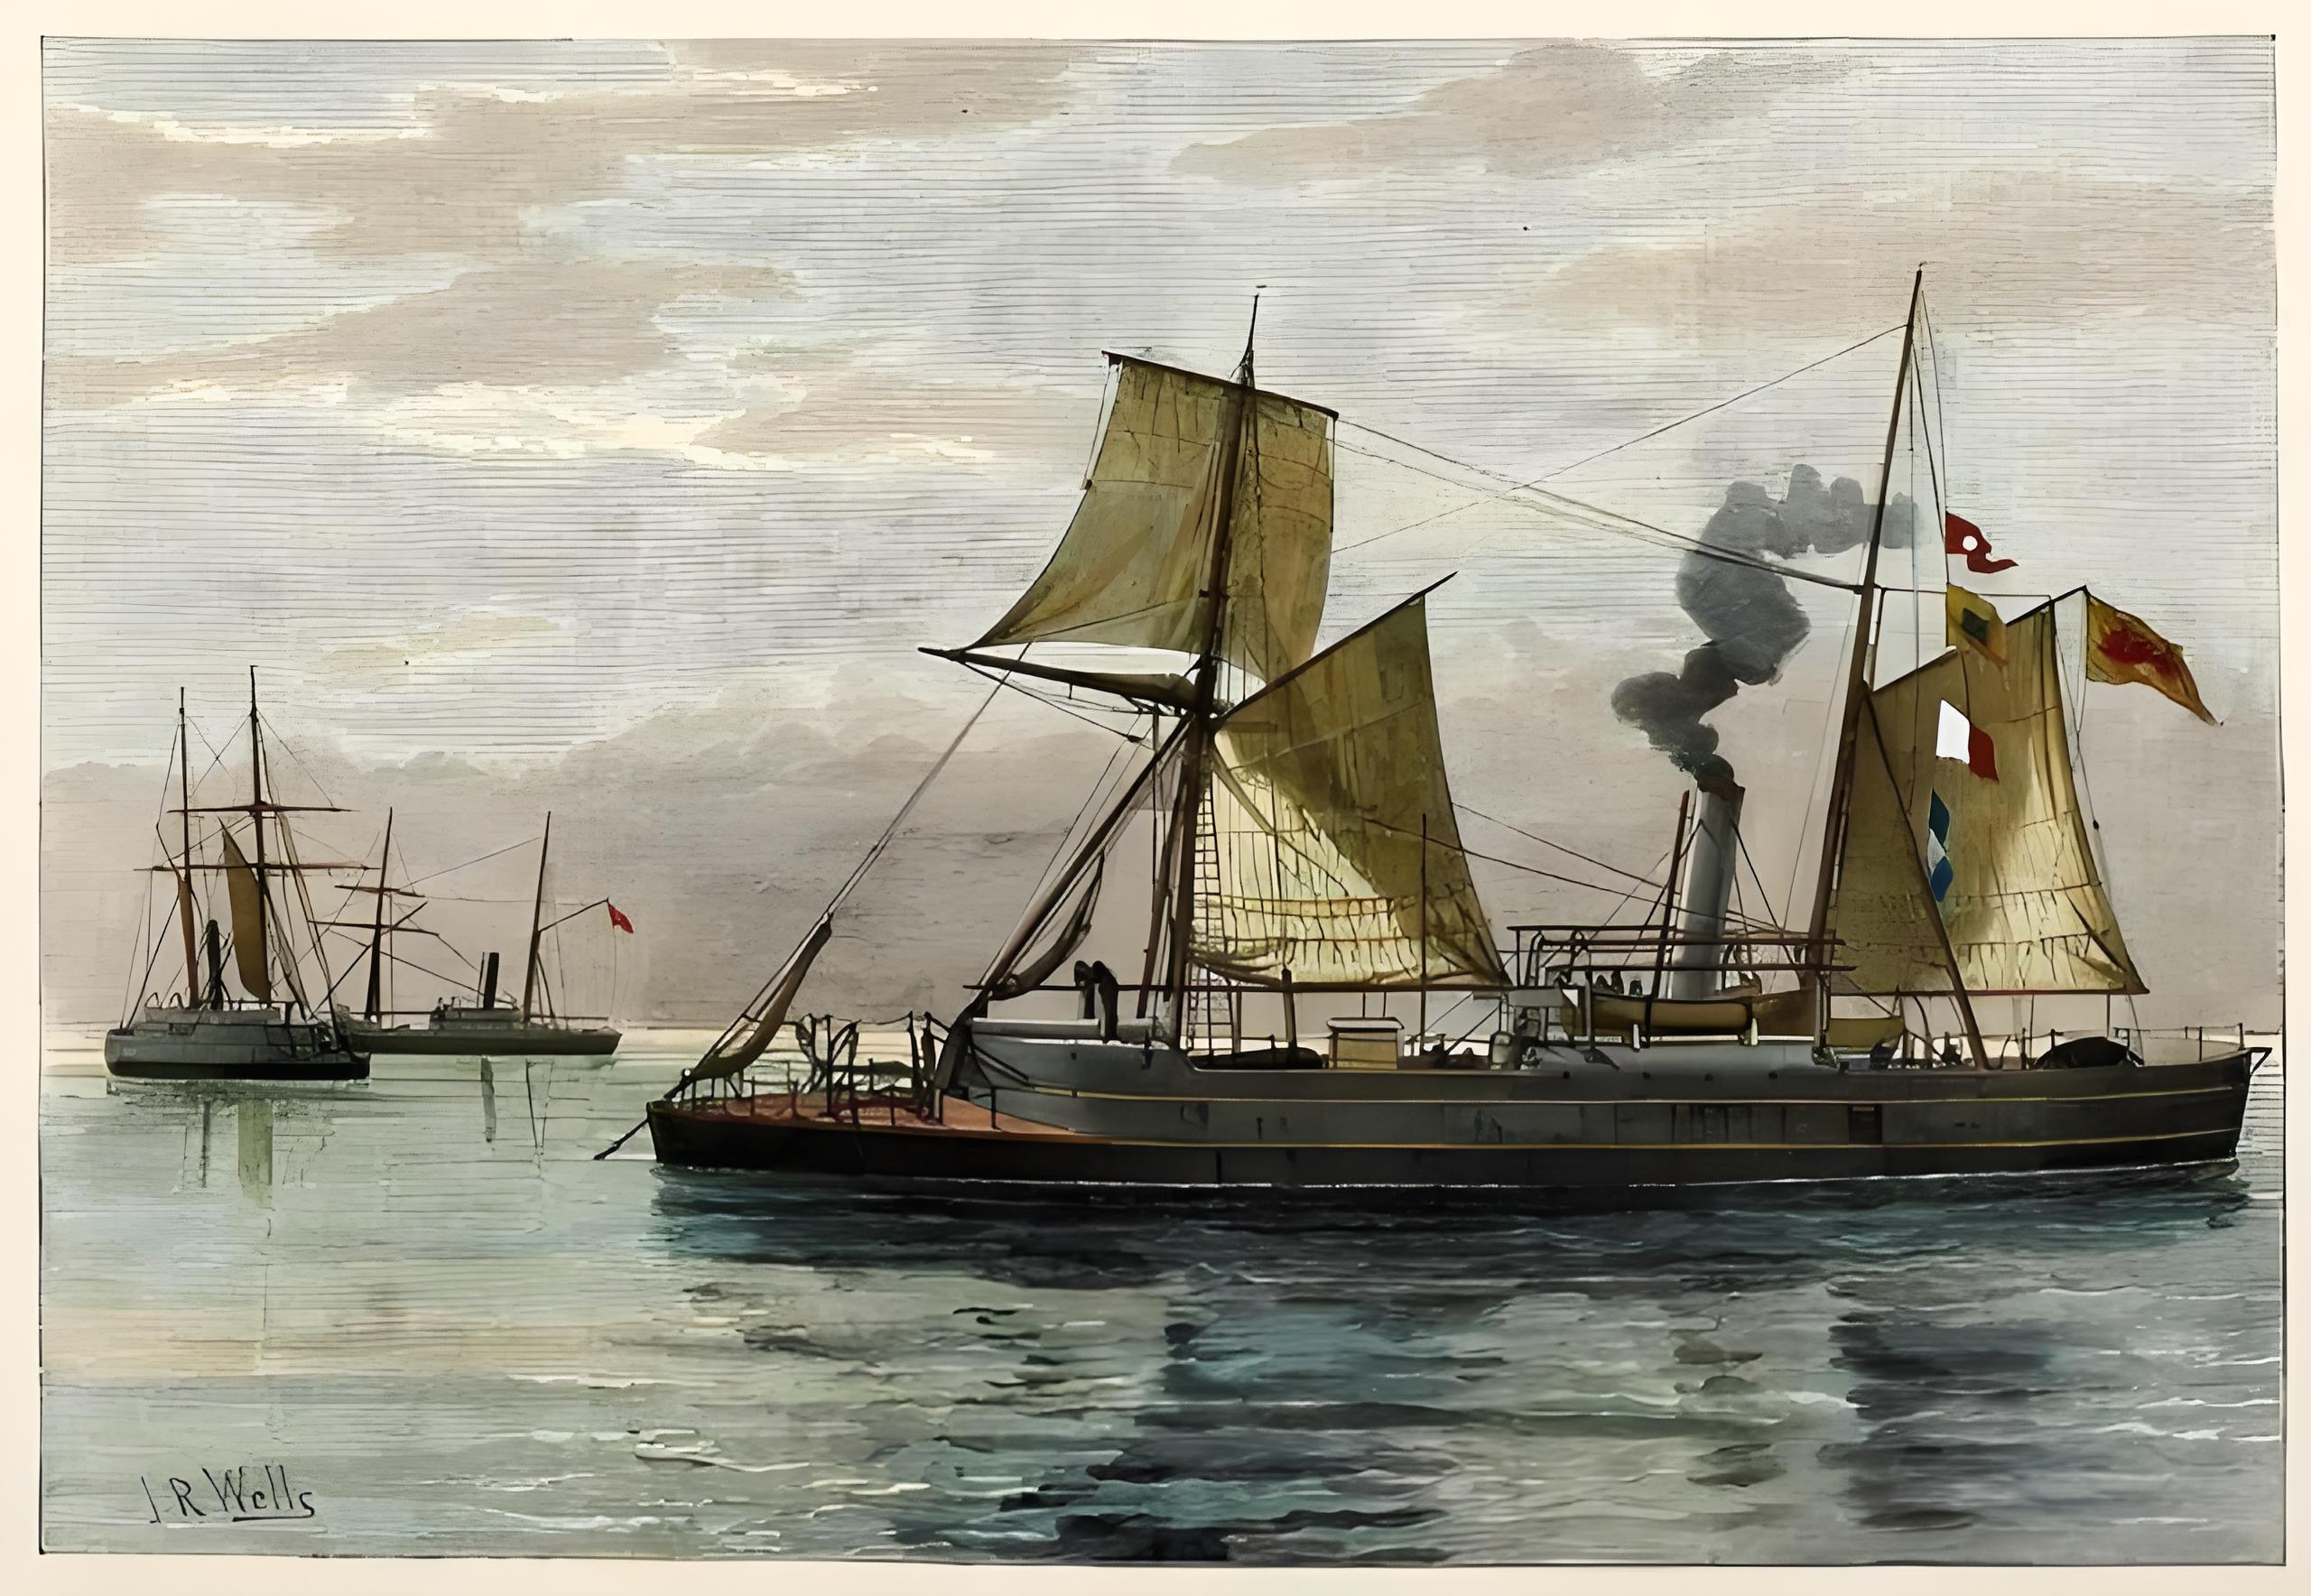
\includegraphics[width=1\linewidth]{Images/11}
	\caption{西方报纸刊载的中国蚊子船编队铜版画。蚊子船回国之初,在基本没有近代化海军基础的情况下,一度成为中国海上武装的骨干,频繁在近海出现、游弋。}
	\label{fig:1}
\end{figure}

清政府最初做出这次增购蚊子船的决策,主要是考虑到南洋大臣提出的加强南洋海防的请求,而原先购买的“龙骧”、“飞霆”等4艘军舰数量太少,不够分拨。因而,“埃普西隆”级蚊子船的订购,虽然经李鸿章之手操办,南洋大臣沈葆桢认为这些军舰将来非南洋莫属,当新式蚊子船到达中国领海后,沈葆桢亲自为四艘军舰命名为“镇北”、“镇南”、“镇西”、“镇东”(Chen Pei、Chen Nan、Chen His、Chen Tung,因而这批军舰又可以称为“镇北”级),且预备派出船政后学堂的毕业生刘步蟾等接管,就任新军舰的管带,在福州马尾等待接收新蚊子船。出乎沈葆桢预料的是,早在订立购舰合同时,李鸿章就意味深长地强调4艘新军舰必须抵达天津大沽,由他自己验收交货。为此,李鸿章还专门通过赫德,派赫德的内弟——江海关税务司赫政(James H.Hart)前往广东,抢在南洋之前迎护,一路监督新蚊子船到达天津。当年11月19日,李鸿章亲自前往大沽检阅4艘新舰,颇为满意。\footnote{中国近代史资料丛刊《洋务运动》2,上海:上海人民出版社1961年版,第418--419页。}

11月30日,李鸿章致信沈葆桢,将“龙骧”、“虎威”、“飞霆”、“策电”4艘较早购买的蚊子船调归南洋,而新购的4艘“镇”字舰留在北洋使用。\footnote{《复两江制军沈》,《李鸿章全集》32,合肥:安徽教育出版社2008年版,第493页。}书信中,李鸿章阐述了他的理由主要有2点,首先“龙骧”等蚊子船在北洋驻防已经2年,原本就需要南下上海进船坞刮修船底,将这4艘军舰调给南洋,“藉省往返”。另外,南洋预备用蚊子船驻防在长江内的吴淞、江阴,“风浪少平”,而北洋的蚊子船需要在大连湾等处航行,“镇”字蚊子船的设计改良更适合在北洋航行。对这种容易让人产生汰旧换新,占南洋便宜嫌疑的行为,李鸿章自表态度“非敢择利自卫”。沈葆桢在得到“镇”字蚊子船被调北上的消息后,也曾致信李鸿章,称“知大君子之用心突出寻常万万也。”\footnote{《沈文肃公牍》,扬州:江苏广陵古籍刻印社1997年版,第1338页。}

4艘“镇”字号蚊子船还在回国途中时,日本悍然吞并了中国属国琉球,中国海防形式极为严峻。当时的中国海防,除了自造的一批兵商两用的炮舰外,所能使用的新式军舰只有新购的蚊子船,但这些舰只都只适应近海防御,无法出远海决胜负,清政府内部有关海防的思想开始发生悄然变化,购买新式碰撞巡洋舰、大型铁甲舰的计划被提到议事日程。但于此同时,与赫德私交甚密的恭亲王奕䜣仍在申请购买一批用于防守近海的水炮台——蚊子船,援引李鸿章的奏折,奕䜣提议广东、台湾的港口防御需要各购买2艘;浙江宁波和山东烟台的港口防御需要各购买1艘,并认为“……令该督抚自行定购,似不如径由该大臣一手经理”,“将来各船购到时,并由该大臣验收”\footnote{《光绪五年十一月十三日总理各国事务衙门奕䜣等奏折附片》,中国近代史资料丛刊《洋务运动》2,上海:上海人民出版社1961年版,第427页。},浅眼看来,和南洋的4艘蚊子船一样,大有以为各省买舰为名,行增加北洋海防之实。

清政府随即同意了恭亲王增购蚊子船的奏请,指令相关各省自筹资金,认真办理,山东巡抚周恒祺很快便认购了2艘蚊子船。而两广总督刘坤一的回复则颇为勉强,环顾左右而言他,最后提出了“造舰”的主张。这年冬天,广东先斩后奏,批准完全由广东机器局总办温子绍个人捐款和设计,在广东黄埔船坞开工仿造一艘蚊子船。\footnote{《刘忠诚公遗集》,台北:台湾文海出版社1973年版,第2089--2095页。}这艘后来命名为“海东雄”(Hai Tung Hung)的军舰,设计上参考了北洋购买的“镇北”级蚊子船,排水量与其相同,为430吨,舰长也一致,同为38.1米,船宽略微增加,为9.14米,吃水2.41米,动力系统采用复合式蒸汽机,航速仅有7.5节。船头装备1门11英寸口径后膛炮,另外配备2门2.75英寸后膛副炮,全舰造价仅为3.39万两银。按照温子绍的设计,“海东雄”不采用英制蚊子船木壳船体外包裹铁皮的做法,直接采用纯木壳,只在部分重要部位敷设铁皮装甲,这样可以避免锈蚀,又可以节省工料节约经费,而且减轻船的吨重,使航行更为便捷。另外,“海东雄”舰艏的火炮改为后膛炮,不光装填方便,而且重量比前膛炮大大减轻,增加了船的稳性,也降低了发射时的后坐力。刘坤一以此为例,申请国家拨款再自造一艘同样的蚊子船,以替代购舰的方案。\footnote{Conway's All The World's Fighting Ships 1860-1905,Conway Maritime Press 1979,p399.}孰料这个建议被驳回,两广最后被迫也认购1艘蚊子船。

\begin{figure}[htbp]
	\centering
	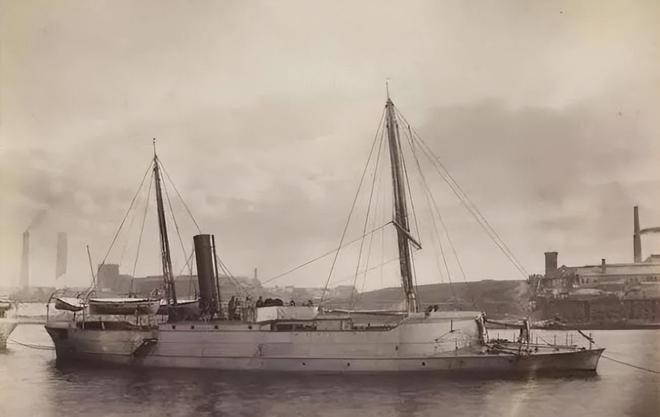
\includegraphics[width=1\linewidth]{Images/12}
	\caption{停泊在纽卡斯尔港边的“约塔”“镇边”舰,可以注意这级舰区别于“埃普西隆”的重要特征——前桅杆上只有一根横桁。}
	\label{fig:1}
\end{figure}

\begin{figure}[htbp]
	\centering
	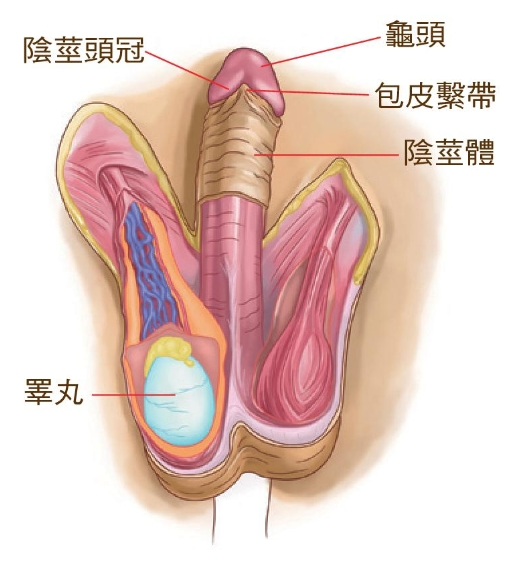
\includegraphics[width=1\linewidth]{Images/13}
	\caption{在英国船坞里进行舾装的中国蚊子船,可能是“镇中”或“镇边”。照片中能清楚看到船艏水线下的舵叶、主炮围壁上的龙纹,以及从“埃普西隆”级开始,依据琅威理的建议在主炮围壁顶上加装的防浪板。}
	\label{fig:1}
\end{figure}

仍然由赫德经手,中国向阿姆斯特朗公司又订购了3艘蚊子船,临时用希腊文字母命名为“约塔”“卡帕”“兰姆达”(Iota、Kappa、Lambda),船体仍然由劳沃克船厂建造,工厂编号411、412、413,于1880年6月2日同时开工,同年12月9日、31日、22日分别下水,1881年4月通过航试。\footnote{Peter Brook:Warships for Export-Armstrong Warships 1867-1927,1999,p31.}由山东付款的前2艘后来被分别命名为“镇中”、“镇边”(Chen Chung、Chen Pien);两广心不甘情不愿认购的那艘,后来被命名为“海镜清”(Hai Ting Ching)。

3艘船为同级,外形各项参数和此前北洋购买的“镇北”级基本相同,外形上主要的区别是,这级军舰前桅杆只有一根横桁,不同于之前中国外购的其他蚊子船。这型蚊子船排水量500吨,长38.1米,宽8.84米,吃水2.9米,动力系统采用2台霍索恩公司造蒸汽机、2台燃煤锅炉,双轴推进,功率455马力,航速10.4节,武备则和“镇北”级完全一样。\footnote{Conway's All The World's Fighting Ships 1860-1905,Conway Maritime Press 1979,p399.}

1881年夏,3舰建造完毕由英国水手驾驶回中国,7月25日到达广州时,“海镜清”被两广留用,而剩下原本由山东订购的“镇边”、“镇中”则在8月11日抵达大沽后,不出所料,被借调北洋水师使用。由此,中国的海防队伍中,共出现了15艘蚊子船。

\begin{figure}[htbp]
	\centering
	
\includegraphics[width=1\linewidth]{Images/14}
	\caption{“约塔”级蚊子船艉部照片,可以看到装饰于船艉的龙纹以及船底侧面的舭龙骨。}
	\label{fig:1}
\end{figure}

\begin{figure}[htbp]
	\centering
	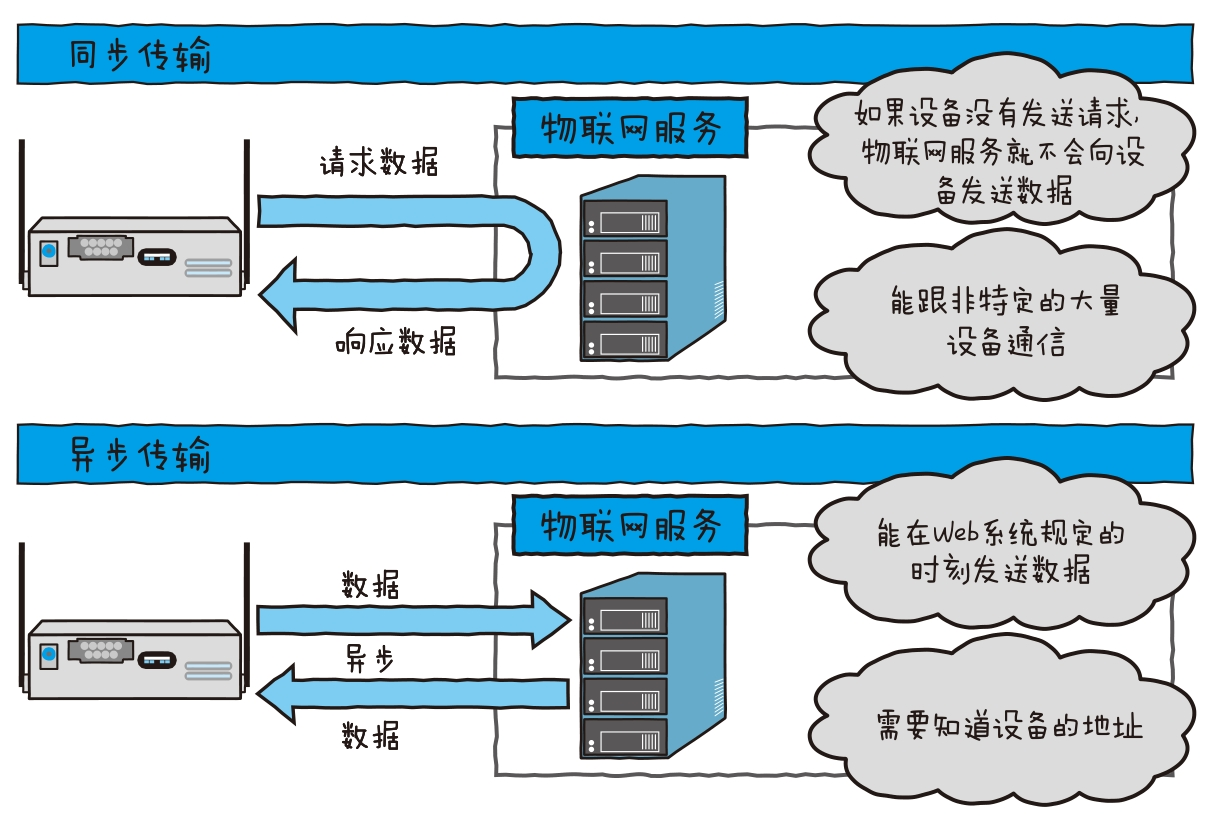
\includegraphics[width=1\linewidth]{Images/15}
	\caption{“约塔”级蚊子船的主炮位。}
	\label{fig:1}
\end{figure}

\begin{figure}[htbp]
	\centering
	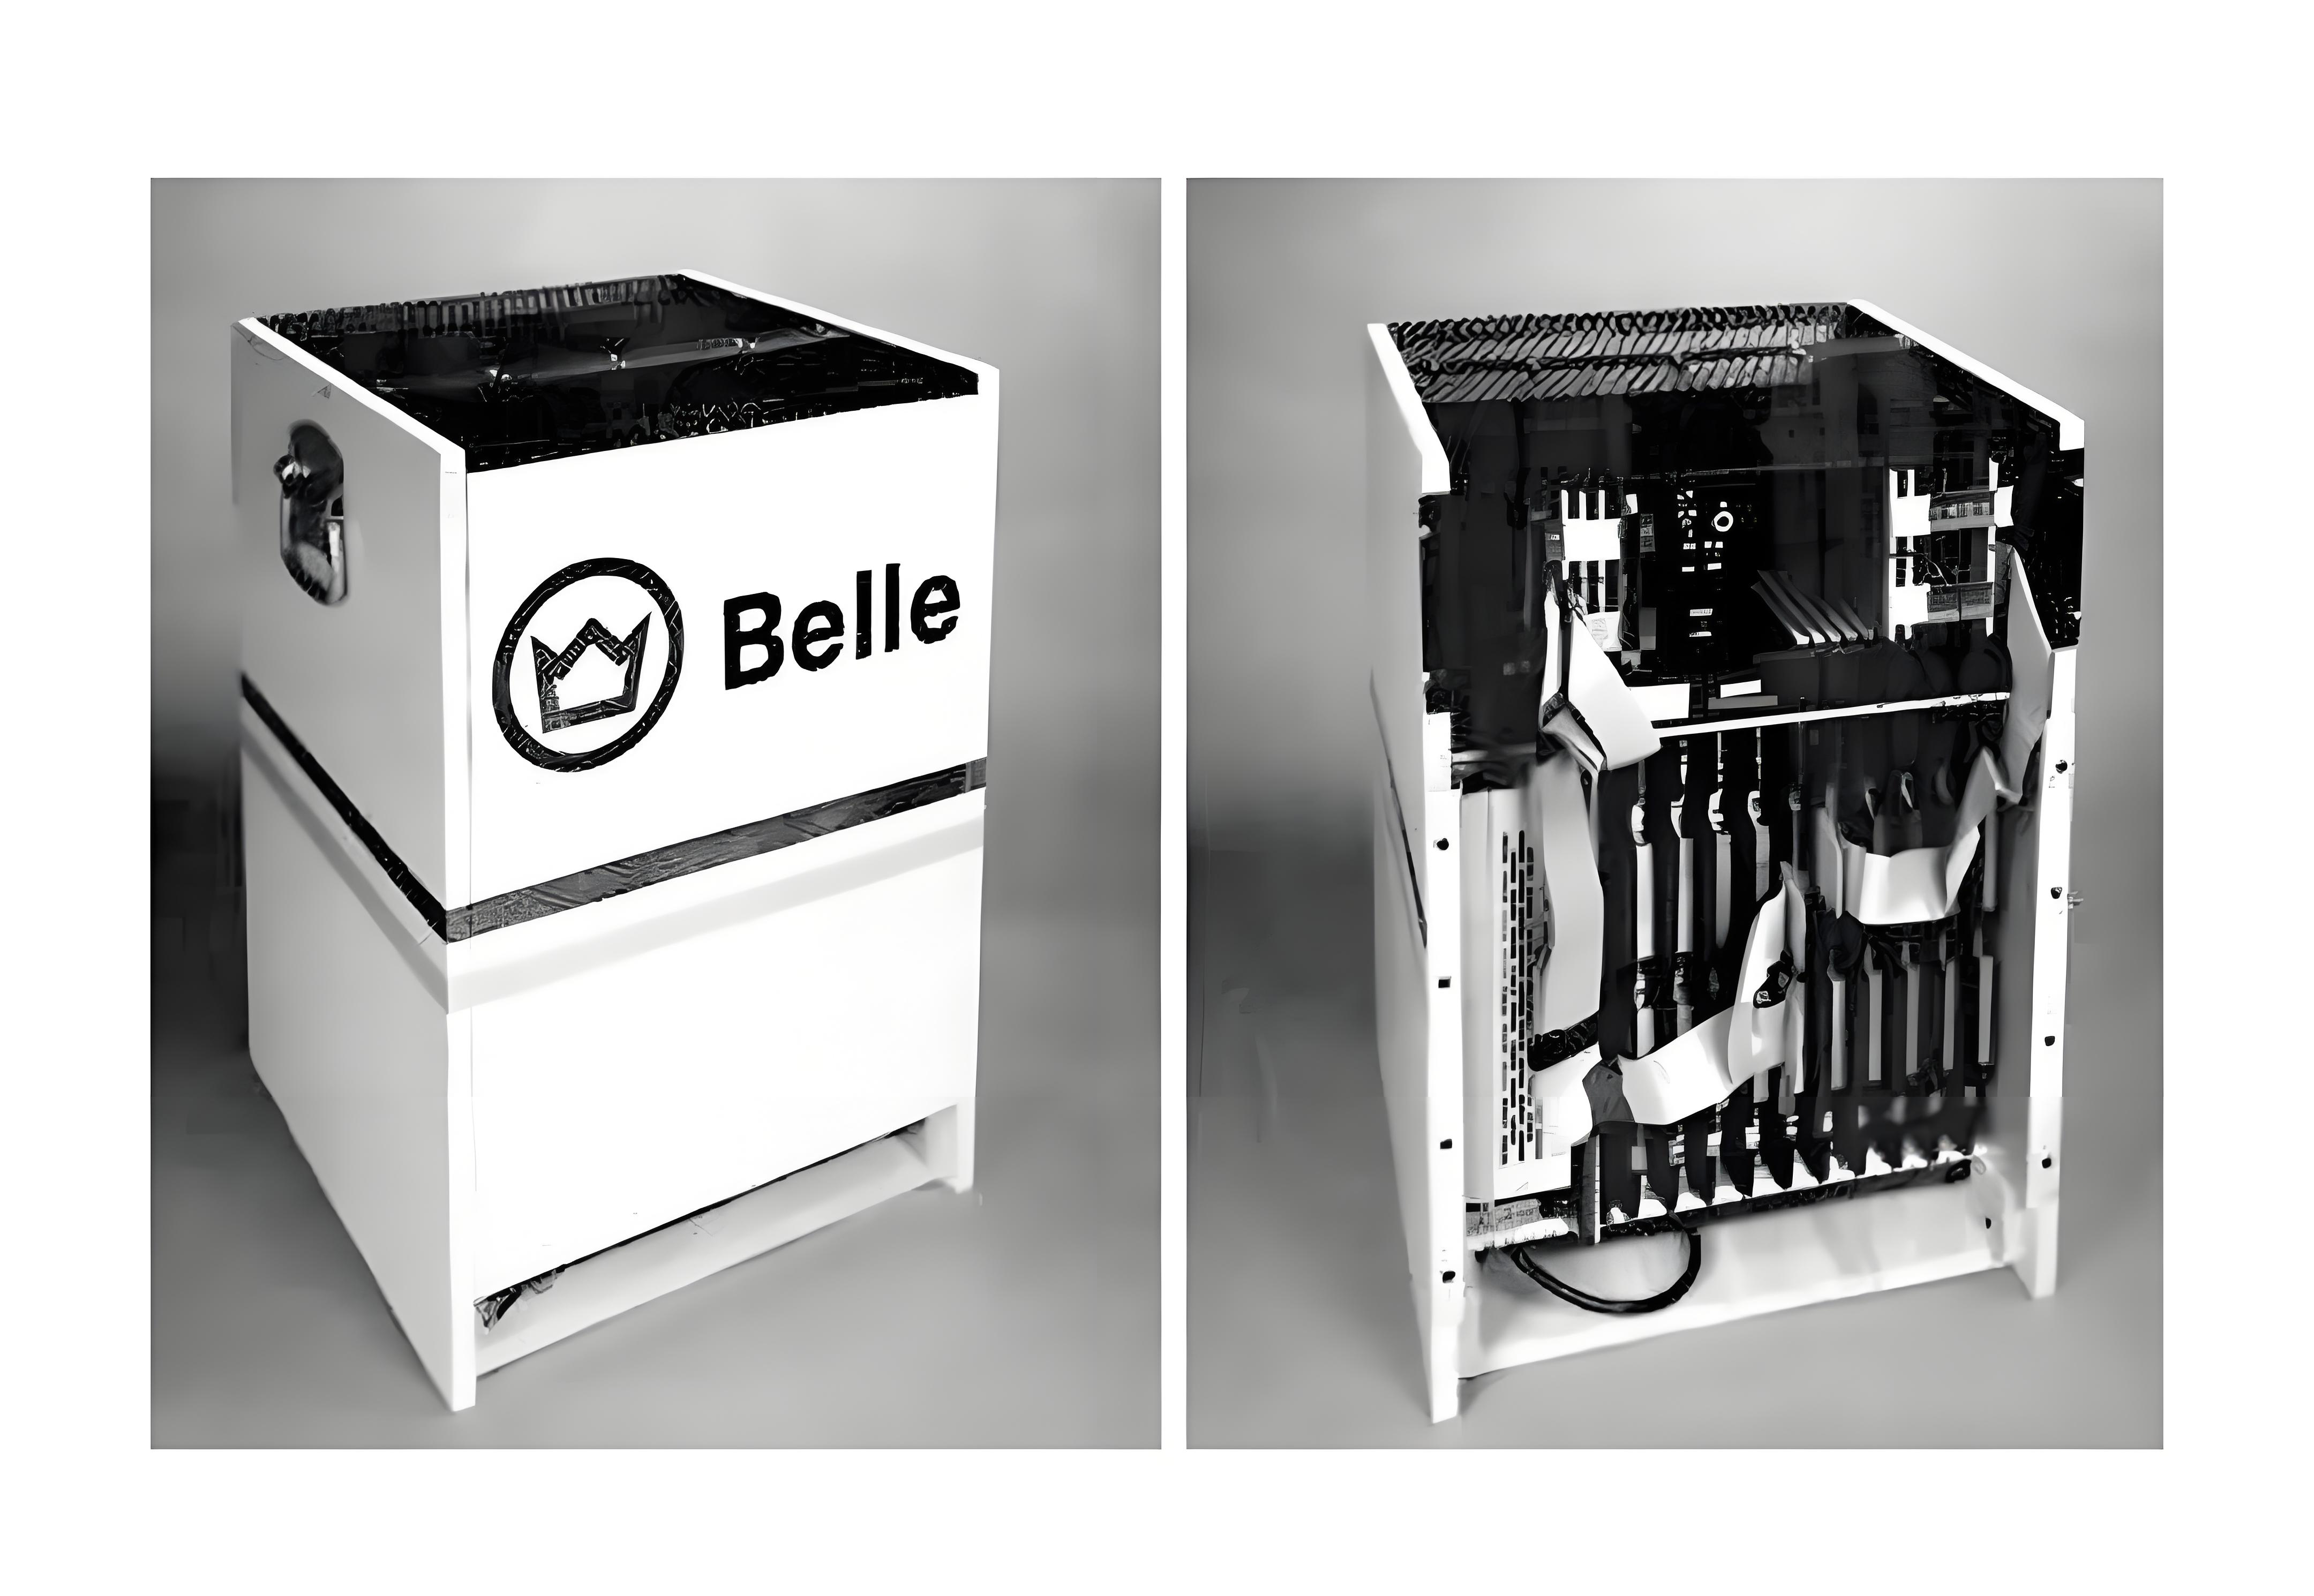
\includegraphics[width=1\linewidth]{Images/16}
	\caption{“约塔”级蚊子船艉部天棚下特写,可以看到安装于艉部的3英寸口径副炮。}
	\label{fig:1}
\end{figure}

\section{龙旗飘零}

4艘“镇北”级蚊子船以及之后并入的“镇中”、“镇边”,在北洋水师里统称六镇炮船。他们回国之初,适逢北洋水师创办,百事待举,在几乎没有任何先进军舰的北洋海防里,用于近海防御的蚊子船成了骨干力量,刘步蟾、林泰曾、邓世昌等后来北洋海军的高级将领,在被李鸿章从福建抽调到北洋的早期,大都出任了各艘蚊子船的管带职务,小小的蚊子船,为中国近代海将走向海洋,提供了历练、磨砺的平台。

随着1879年琉球事件、1884年中法战争的刺激,清政府对于海军、海防又有了更深刻的认识,很快看到早期购买的蚊子船对于舰种齐全的海军大国,尚有守护海口,独当一面的意义。而像中国这样几乎没有任何海军装备基础的国家,花重金购买这批军舰,并不能对增加国家的海上力量尤其是远海机动力量有多少帮助,潜移默化中,李鸿章的海防观由近海守口防御,悄然向远海改变。先是向英国订购了2艘新型的撞击巡洋舰“超勇”、“扬威”,之后更是购办了威震东亚的大型铁甲舰“定远”、“镇远”,这些大型军舰回国后,中国海军开始频繁活跃在北起海参崴,南至新加坡的辽阔海域,只能用于近海守口的蚊子船,逐渐显得不再重要,为节省经费起见,北洋海防的6艘蚊子船每年只维持2艘在海上值勤,剩余4艘则收入船坞封存,相关的人员并入铁甲舰服役,昔日世界名舰的光彩逐渐黯淡。

1894年夏,中日两国爆发甲午战争。战争开始后不久,北洋所有蚊子船全部予以启用,重新编制人员,再度活跃于近海,主要负责防护威海、旅顺等要港。9月16日,护送陆军前往大东沟登陆的北洋海军主力队伍中,也有2艘蚊子船“镇中”、“镇南”的身影,当时它们的主要任务是守护在大东沟口,防止日本舰队偷袭入口,因而并未参加著名的黄海大东沟大战,只是在海战后期曾响应“靖远”舰挂出的旗号,配合北洋幸存各舰一起收队。

进入1895年,战火逐渐蔓延到北洋海军的重要基地威海刘公岛,作为守港利器的6艘“镇”字号蚊子船参与了惨烈的威海保卫战,北洋海军数度打退日本舰队海上进攻的战斗中,蚊子船的作用功不可没。然而,随着威海湾陆地炮台的接连失守,北洋海军陷入四面楚歌的困境,大舰纷纷受创沉没。

\begin{figure}[htbp]
	\centering
	
\includegraphics[width=1\linewidth]{Images/17}
	\caption{正在运送刘公岛降军出岛的“镇东”级蚊子船。}
	\label{fig:1}
\end{figure}

\begin{figure}[htbp]
	\centering
	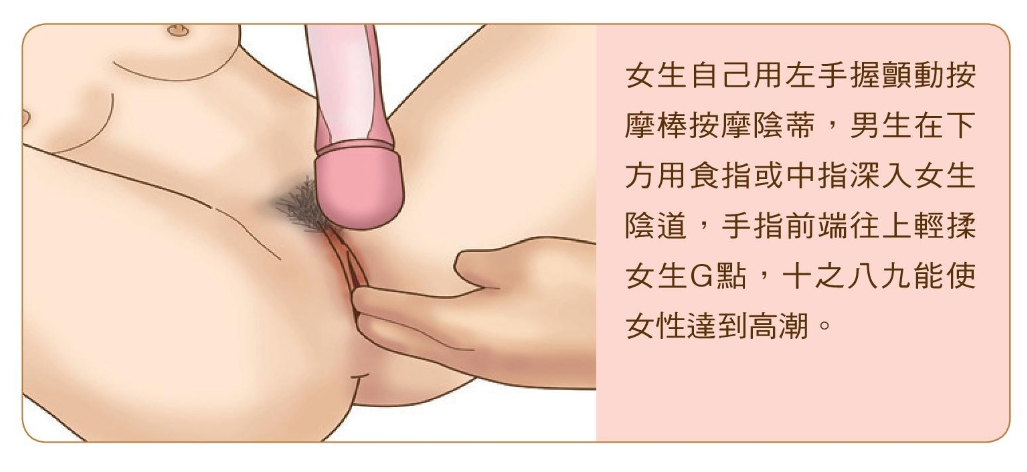
\includegraphics[width=1\linewidth]{Images/18}
	\caption{停泊在旅顺的被俘蚊子船。}
	\label{fig:1}
\end{figure}

2月12日上午8时,中国发展近代海军最早努力的成果、曾经的“埃普西隆”号“镇北”舰悬挂白旗,载着特使程璧光,缓缓驶向日本舰队锚地接洽投降。2天后,北洋海军投降,全军覆没,全岛官兵5124人被日军遣返,残存的6艘“镇”字蚊子船承担了运送刘公岛上官兵离岛的悲惨任务。

\begin{figure}[htbp]
	\centering
	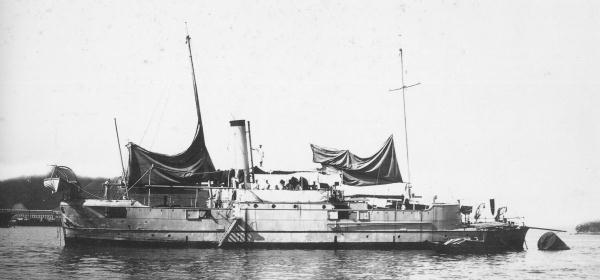
\includegraphics[width=1\linewidth]{Images/19}
	\caption{编入日本海军的“镇中”舰,1897年拍摄于日本吴港。}
	\label{fig:1}
\end{figure}

\begin{figure}[htbp]
	\centering
	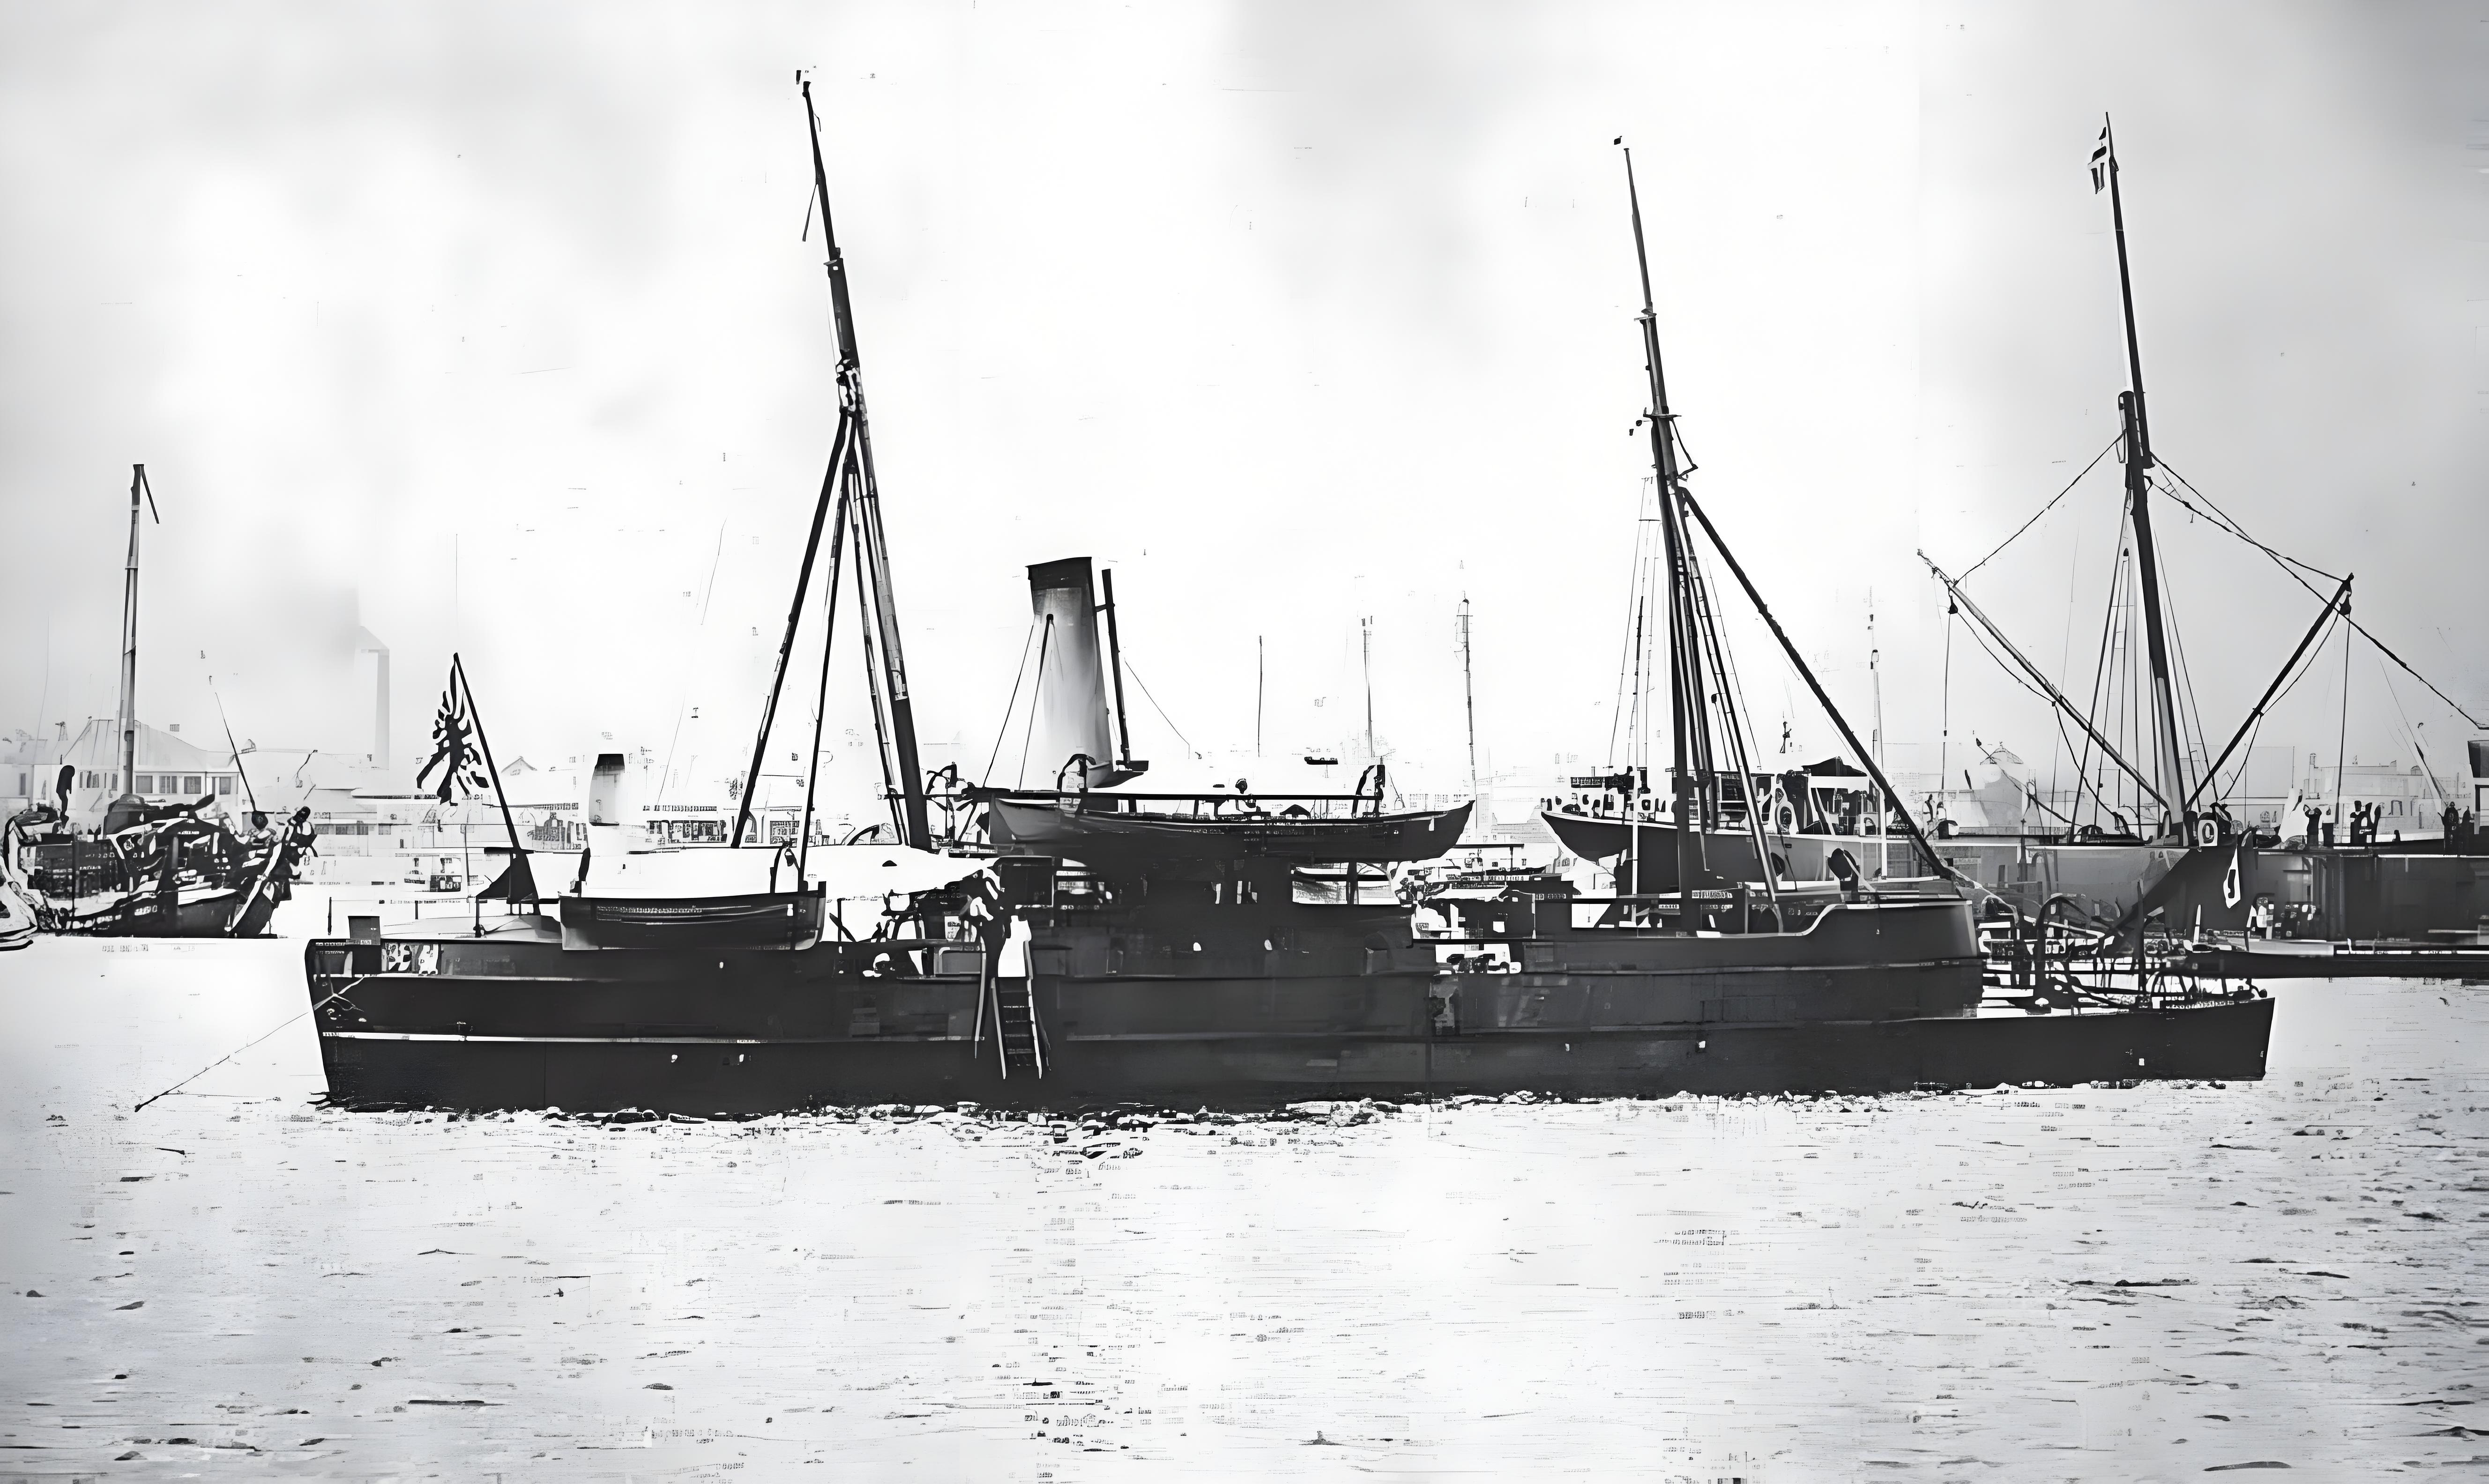
\includegraphics[width=1\linewidth]{Images/20}
	\caption{被俘未久的“镇北”舰,舰艉还可以清晰看到中文舰名牌。}
	\label{fig:1}
\end{figure}

\begin{figure}[htbp]
	\centering
	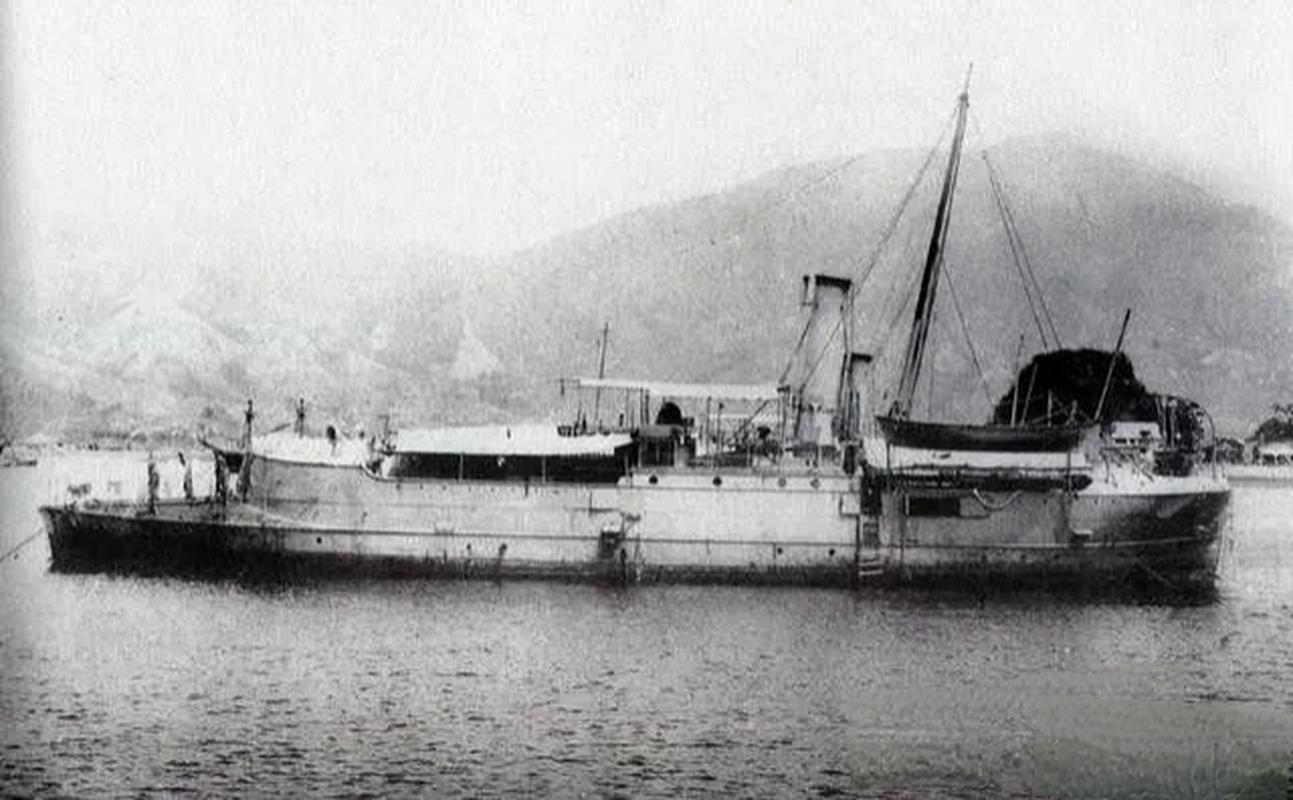
\includegraphics[width=1\linewidth]{Images/21}
	\caption{成为日本军舰的“镇边”,1897年拍摄于神户。}
	\label{fig:1}
\end{figure}

\begin{figure}[htbp]
	\centering
	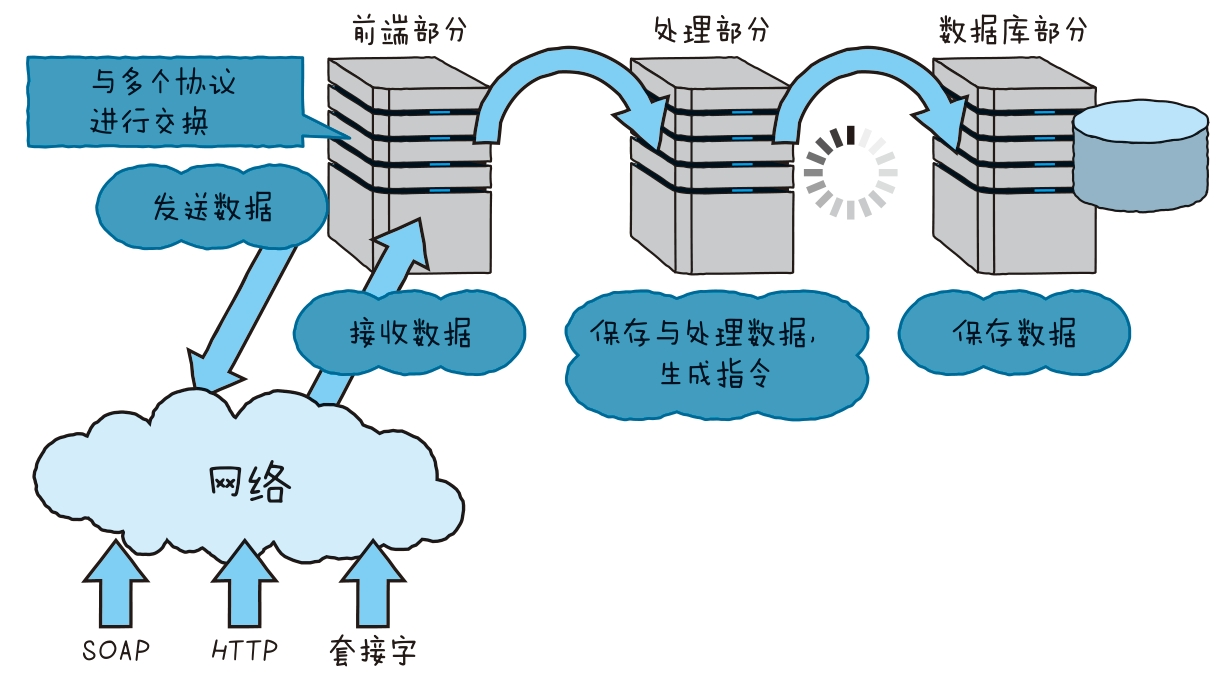
\includegraphics[width=1\linewidth]{Images/22}
	\caption{编入日本海军后的“镇西”舰。}
	\label{fig:1}
\end{figure}

从此,“镇”字号蚊子船被编入了日本海军,长期充当一些无关紧要的角色。

1898年3月21日6艘蚊子船集体被定为二等炮舰级,1903年8月21日一同除籍成为杂役船。

其中“镇东”舰1906年6月8日报废、1907年转售。“镇南”舰1908年5月15日报废,于1913年转售。“镇西”舰于1908年5月23日转归文部省所有。“镇北”舰1906年6月8日报废,,1909年转售。“镇中”与“镇边”两舰由于船龄较新,在1900年庚子事变时作为八国联军海军的成员被派在大沽口外巡逻,两舰最后同在1906年6月8日报废,“镇中”舰于1909年转售,“镇边”舰同年7月16日改归司法省所有。

北洋海军的蚊子船,这些未能执行任何与他们职能相称的使命的军舰,就这样来去匆匆地消逝在历史长河中。

\begin{quotation}
	东南归路莽萧条,皖口千峰若为招。
	
	半局残棋存战舰,八年恨事付寒潮。
	
	灵风下水征帆疾,落日中原汉马骄。
	
	孤客不堪回首望,断云一片劫灰烧。
	
	\begin{shuming}
	——李鸿章《登小姑山感怀》
	\end{shuming}
	
\end{quotation}

\chapter{纽卡斯尔的梦——“超勇”级撞击巡洋舰}

清冽的海风从泰恩河(River Tyne)掠过,带来北海上独特的气息,薄雾渐渐散去,大英帝国的纽卡斯尔(Newcastle)军港里呈现出满目繁忙景象。岸上一队队水手、士兵来来往往,川流不息,为码头旁两艘外形秀丽的军舰运输着补给。指挥的银笛声、搬运重物的号子声、军舰发出的悠长汽笛声,共同奏响了一曲醉人的起航之歌。人群中,有名穿着蓝色制服,腰挎军刀的年轻海军军官静静地伫立着,凝视远方的目光中透出一股深情。

一位俏丽的金发少女翩然而至,给忙碌的码头带来一丝不小的波动。周围的人们纷纷抬头观望、窃窃私语,间或有几张面孔露出会心的笑容。少女手中捧着芳香四溢的蛋糕,上面写着“The Imperial Chinese Navy-Chao Yung”(大清帝国海军——“超勇”)和一个显然是属于东方人的名字。顾不得平静一下呼吸、拭去额头的汗珠,少女走向那位年轻军官,两人的身影俨然成了纽卡斯尔这个夏天最美的风景。

“……告别黯然魂销,不忍长辞……意腻(Annie Fenwick)自制香糕罩以雪糖,作船名及余名,冠以吉祥语,又知余家有母,自制食物一瓶,书送慈亲,嘱余转奉,闻者尤感之,况余身受者乎……匆匆一别,再晤何期,未免有情,谁能遣此矣……”\footnote{池仲祐:《西行日记》,北京:商务印书馆1908年版,卷下第10--11页。}

1881年8月9日,中国海军“超勇”、“扬威”号巡洋舰从纽卡斯尔起航回国。

\section{新式巡洋舰}

“……保密——目前海军一般人的意见和炮术的进步越来越对装甲舰不利。阿姆斯特朗公司已设计出新式非装甲巡洋舰,时速15海里,排水量1200吨,吃水15英尺,机器被水下舱板遮蔽,用煤堆保护。装备两门25吨新型后膛炮,足以穿透海上的任何铁甲舰,一门安装在舰艏,一门在舰艉,均绕枢轴旋转,可向前方和舷侧目标射击。此外尚有小炮及鱼雷装置。全舰水手七十人。建造时间十五个月,全部造价90000镑。所有以上各项数字均系估计的近似值。此种巡洋舰将被证明比现存各种巡洋舰优越,就像‘阿尔法’、‘伽马’型号炮艇之优于其他炮艇一样,它将成为新型炮艇的重要补充。这是您的理想从炮艇级扩展到巡洋舰级,如在别国政府之前被中国政府所采用,您将再一次在海军科学方面居于领先地位……”\footnote{《金致赫第257号》,《中国海关密档》8,北京:中华书局1995年版,第177页。}

1879年6月15日,这份电报由英国伦敦经恰克图电报线,传递到中国海关总税务司位于北京的办公桌上。发报者是中国海关驻伦敦办事处主任金登干,收件人则是在中国近代史上大名鼎鼎的赫德爵士。这位出生于爱尔兰的英国人,19岁时作为一名对华外交人员踏进了这个神秘的东方国度,因为好学、工作勤勉、处事积极,28岁时就荣登中国海关总税务司的宝座,并一直担任至76岁的耄耋老年,几乎把一生的时光都驻留在了中国。在职期间以其特有的热情、认真精神,使海关成为当时中国官僚机构中效率较高、较廉洁的部门,海关新税也成为了清末中国政府财政收入的重要来源。曾经竖立在上海外滩的铜像,象征了他在这个国家历史上留下的独特印记。

\begin{figure}[htbp]
	\centering
	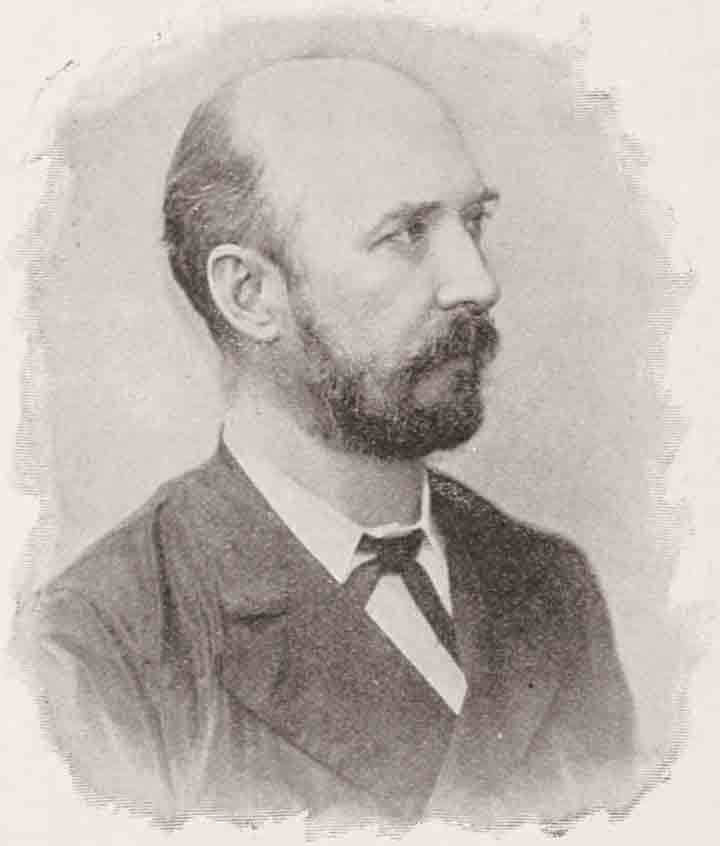
\includegraphics[width=1\linewidth]{Images/23}
	\caption{中国海关总税务司赫德。}
	\label{fig:1}
\end{figure}

可能是源自岛屿民族性格里那鼓对大海与生俱来的热情,作为英国在华利益的代言人和攫取者,赫德在控制中国海关行政管理权,干涉中国内政的同时,对于中国创建近代海军的计划也颇感兴趣。早在1861年,赫德就参与了“李泰国-阿思本舰队”的筹划、谈判,是为其介入中国海防事务的最早实践。1874年日本侵台事件发生后不久,关于建设西式海军的提案重新引起清政府重视,赫德借此再度插足中国海军建设领域,通过与北洋大臣李鸿章的反复讨论,掀起了大规模购买西方军舰的浪潮。

实际上,赫德本人对海军、军舰并无太深了解,他的有关信息和知识大都得自中国海关驻伦敦办事处主任金登干,而这个办事处的一项重要任务正是为中国联系购买军火、舰船。早期促成中国购买了一批蚊子船,使得赫德越发意气风发,以致做起了中国海军总司令的美梦,并积极鼓动中国购买更大的军舰,借以一步步实现英国对中国海军的影响(赫德一度曾向清政府提出设立海防总署,由其出任总海防司的设想,以便直接控制中国的新式海军。后经南洋大臣沈葆桢、北洋大臣李鸿章等极力反对而作罢)。

金登干发来的这份极尽阿谀的电报,介绍了阿姆斯特朗公司新推出的一种巡洋舰,恰好投中赫德的下怀。似乎是觉得电报里说得还不够清楚,5天后,意犹未尽的金登干从伦敦又寄出了一封长信,更为详细地描述新巡洋舰的特性,强调这型用于进攻的巡洋舰,是对中国海军已有蚊子船的极好补充。并认为,对于财政支绌的中国政府而言,与其孤注一掷购买几艘价值不菲的大型铁甲舰,不如用这笔钱来装备一批单价便宜的巡洋舰,而且依据当时英国海军舰船设计界的观点,这种价格低廉的巡洋舰理论上还是大型铁甲舰的克星,为了论证铁甲舰很快会被淘汰,金登干举了个生动的例子,“……这个题目可以作无限引申的详细阐述,比如说,人身铠甲的废置不用就是一个恰当的例证……”\footnote{《中国海关密档》2,北京:中华书局1995年版,第205页。}

电报中提到的巡洋舰,依据十九世纪海军的分类标准,属于碰撞巡洋舰(Ram Cruiser)或撞击巡洋舰,中国史料称为碰船兼快船、碰快船。探寻这类军舰的源头,可以上溯至1866年意大利、奥地利两国之间爆发的利萨海战。那次海战中,由特格特霍夫(Wilhelm von Tegetthoff)海军上将率领的奥地利舰队列成横阵(或称楔型阵、“人”字阵,中国称雁行阵),大败采取纵队的意大利舰队,从而影响了世界海军战术的走向。海战中,奥地利旗舰“斐迪南德·马克思”(Erzherzog Ferdinand Max)将意大利舰队旗舰“意大利国王”(Re D' Italia)拦腰撞沉的经过更是成了海军史上的经典战例。尽管这次成功的撞击中夹杂着太多偶然性因素,然而对沉寂已久的海军战术和舰船设计领域来讲,利萨海战带来了全新的理念和思想,引发了关于船头对敌战术的意义、舰艏方向火力的重要性,以及撞击战术价值的再认识,大转变由此开始。

撞击战术的偶然成功,很快被传成了神话。以至于有人要设计以撞击为主要作战手段的军舰——撞击巡洋舰。始作俑者是英国著名的舰船设计师乔治·伦道尔,因设计小船装大炮的蚊子船而声名鹊起的伦道尔,坚持可以建造一种小而便宜的军舰去战胜和替代昂贵的铁甲舰,这类小型军舰的重要特征是航速快、装有撞角、舰体外形简洁、隐蔽,能够利用其装备的撞角、大口径火炮对铁甲舰构成威胁。这一概念性的理论随即受到追捧,19世纪后期,人们可以在世界各地很多军港里见到这类军舰的身影。

在严峻的海防形势压迫下,中国近代海军建设的初期,对国际上海军技术发展的走向一直保持密切关注,几乎是不错过任何一个新技术,可谓紧追潮流。早期购买蚊子船,以及后来订造铁甲舰、穹甲巡洋舰、装甲巡洋舰,乃至自行设计建造潜水艇、舟桥船、全钢军舰皆是例子。这种对新技术的敏感性,和发展海军的努力,在当时亚洲国家中遥遥领先,即使在世界来讲,也不稍逊色。新锐的概念舰——撞击巡洋舰,通过赫德推荐、介绍后,主持北洋海防建设的北洋大臣、直隶总督李鸿章立刻产生了兴趣。当时,中国海军迫切需要一种堪当重任,能出远海作战的新式军舰,但因为“经费太绌、议论不齐、将才太少”,中国购买铁甲舰作为海军主力的计划一拖再拖,使得主持此事的李鸿章备感压力。现在突然出现了一种价格低廉,且能“追赶碰坏极好之铁甲船”的巡洋舰,无异天赐良机。经详细查看图纸和咨询外国军官后,1879年12月9日,李鸿章委托赫德向英国阿姆斯特朗公司洽谈订造2艘新式撞击巡洋舰。\footnote{《赫致金第113号》,《中国海关密档》8,北京:中华书局1995年版,第190页。}两天后正式向清政府作出奏报,在强调购买巡洋舰的重要性同时,引人注意的是,李鸿章在奏折中称,中国要巩固海防,“非购置铁甲等船练成数军决胜海上,不足臻以战为守之妙”\footnote{《光绪五年十月二十八日直隶总督李鸿章奏折》,中国近代史资料丛刊《洋务运动》2,上海:上海人民出版社1961年版,第421--422页。},表示目前购买巡洋舰只不过是为他日的铁甲舰队做准备,实际并不认同赫德、金登干等人有关铁甲舰过时的论调。

对于中国的委托,赫德认为此项工程完成的好坏将直接影响到对华军火贸易的扩大,以及英国在可以预见的将来对中国海军的影响,于是专门致信给在英具体办理此事的金登干,着重强调军舰在平静水域的标准航速必须超过15节,舰艏要装备特别强有力的弓形撞角,提醒金登干,李鸿章对舰载鱼雷艇抱有浓厚的兴趣,希望鱼雷艇速度必须达到17至18节,并要求2艘军舰要于1881年春季交船。\footnote{《中国海关密档》2,北京:中华书局1995年版,第205页。}

金登干不敢怠慢,立即着手与阿姆斯特朗公司谈判,1879年12月18日正式签订合同,2艘军舰总价16万英镑,低于1艘9万英镑的最初报价。和定造蚊子船时的模式相似,双方约定船价分三次支付,合同签订后的6个月内付第一批,此后6个月内付第二批,竣工后支付余款,期间按年利5%支付过渡期利息。英国丽如银行负责分期付款担保,收取1%担保金。\footnote{《金致赫第286号》,《中国海关密档》8,北京:中华书局1995年版,第192页。}

\section{“超勇” “扬威”}

1880年4月17日,按照合同规定的首批造价汇至中国海关在丽如银行开设的G账户内支付。\footnote{《赫致金第126号》,《中国海关密档》8,北京:中华书局1995年版,第204页。}在此之前,中国的两艘撞击巡洋舰已经在1月15日双双开工,建造编号分别为406、407。\footnote{Peter Brook: Warships for Export-Armstrong Warships 1867-1927,1999,p48.}经金登干提议,赫德将两艘军舰暂时命名为“白羊座(Aries)”和“金牛座(Taurus)”,前者表示两艘军舰都有尖尖的角,后者则寓意军舰的产地是欧洲(西方神话中,天神宙斯曾化身金牛追求人间一位美丽的公主,后来故事的发生地用公主的名字欧罗巴命名,此即传说中欧洲名称的由来)。同年12月27日,李鸿章取“超勇”和“扬威将军”的封号,将两艘军舰正式命名为“超勇”“扬威”,\footnote{《派丁汝昌赴英国收船片》,《李鸿章全集》9,合肥:安徽教育出版社2008年版,第237--238页。}英文译名Chao Yung、Yang Wei,遵从西方海军的习惯,两艘同型舰可以并称为“超勇”级。

阿姆斯特朗(William George Armstrong,1810--1900)开创的阿姆斯特朗公司,是近代世界著名的火炮制造商,当时并没有自己单独的船厂,承揽的造船业务,船体部分都是转包给位于泰恩河畔的劳沃克船厂建造,中国的这两艘巡洋舰也不例外。当时在劳沃克船厂内,还有一艘已经开工的同型巡洋舰,即智利政府订造的Arturo Prat号,后来这艘船一度准备转卖给中国,但被李鸿章回绝,于1883年被日本购得,更名为“筑紫”。值得一提的是,出于多种考虑,赫德对于2艘巡洋舰的建造质量非常关心,当得知新军舰的舰体不在阿姆斯特朗公司建造时,专门致信金登干,异常详细地询问了米切尔船厂的造船历史、规模、施工能力等细节情况,并多次提醒金登干注意监督,要求必须造出2艘“第一流的巡洋舰”。\footnote{《中国海关密档》2,北京:中华书局1995年版,第276、297页。}

由伦道尔设计的“超勇”“扬威”,在劳沃克船厂的生产编号为406、407,舰型属于撞击巡洋舰,正常排水量1380吨(一说1350吨),满载排水量1542吨,舰长64米,宽9.75米,吃水4.57米。主机采用的是英国霍索恩公司生产的2座卧式往复式蒸汽机,配备6座锅炉(早于“超勇”级建造的智利Artuor Prat号只有4座锅炉,为满足李鸿章对于航速的要求,伦道尔在两艘中国军舰上做出了改进,将锅炉增加到6座),双轴推进。设计功率2600匹马力,航速16节。舰上煤舱正
常储量250吨,最大可以储存300吨。续航能力5380海里/8节。\footnote{Conway's All The World's Fighting Ships 1860-1905,Conway Maritime Press 1979,p396. Peter Brook: Warships for Export-Armstrong  Warships 1867-1927,1999,p48.}除蒸汽动力外,“超勇”级军舰上还配置有帆装,安装有两根桅杆,能采用风帆动力航行,设计时桅杆属于直杆,只能张挂索具相对简单的纵帆。回国后不久,中国方面对桅杆进行了简单改造,在前桅加装了横桁。

\begin{figure}[htbp]
	\centering
	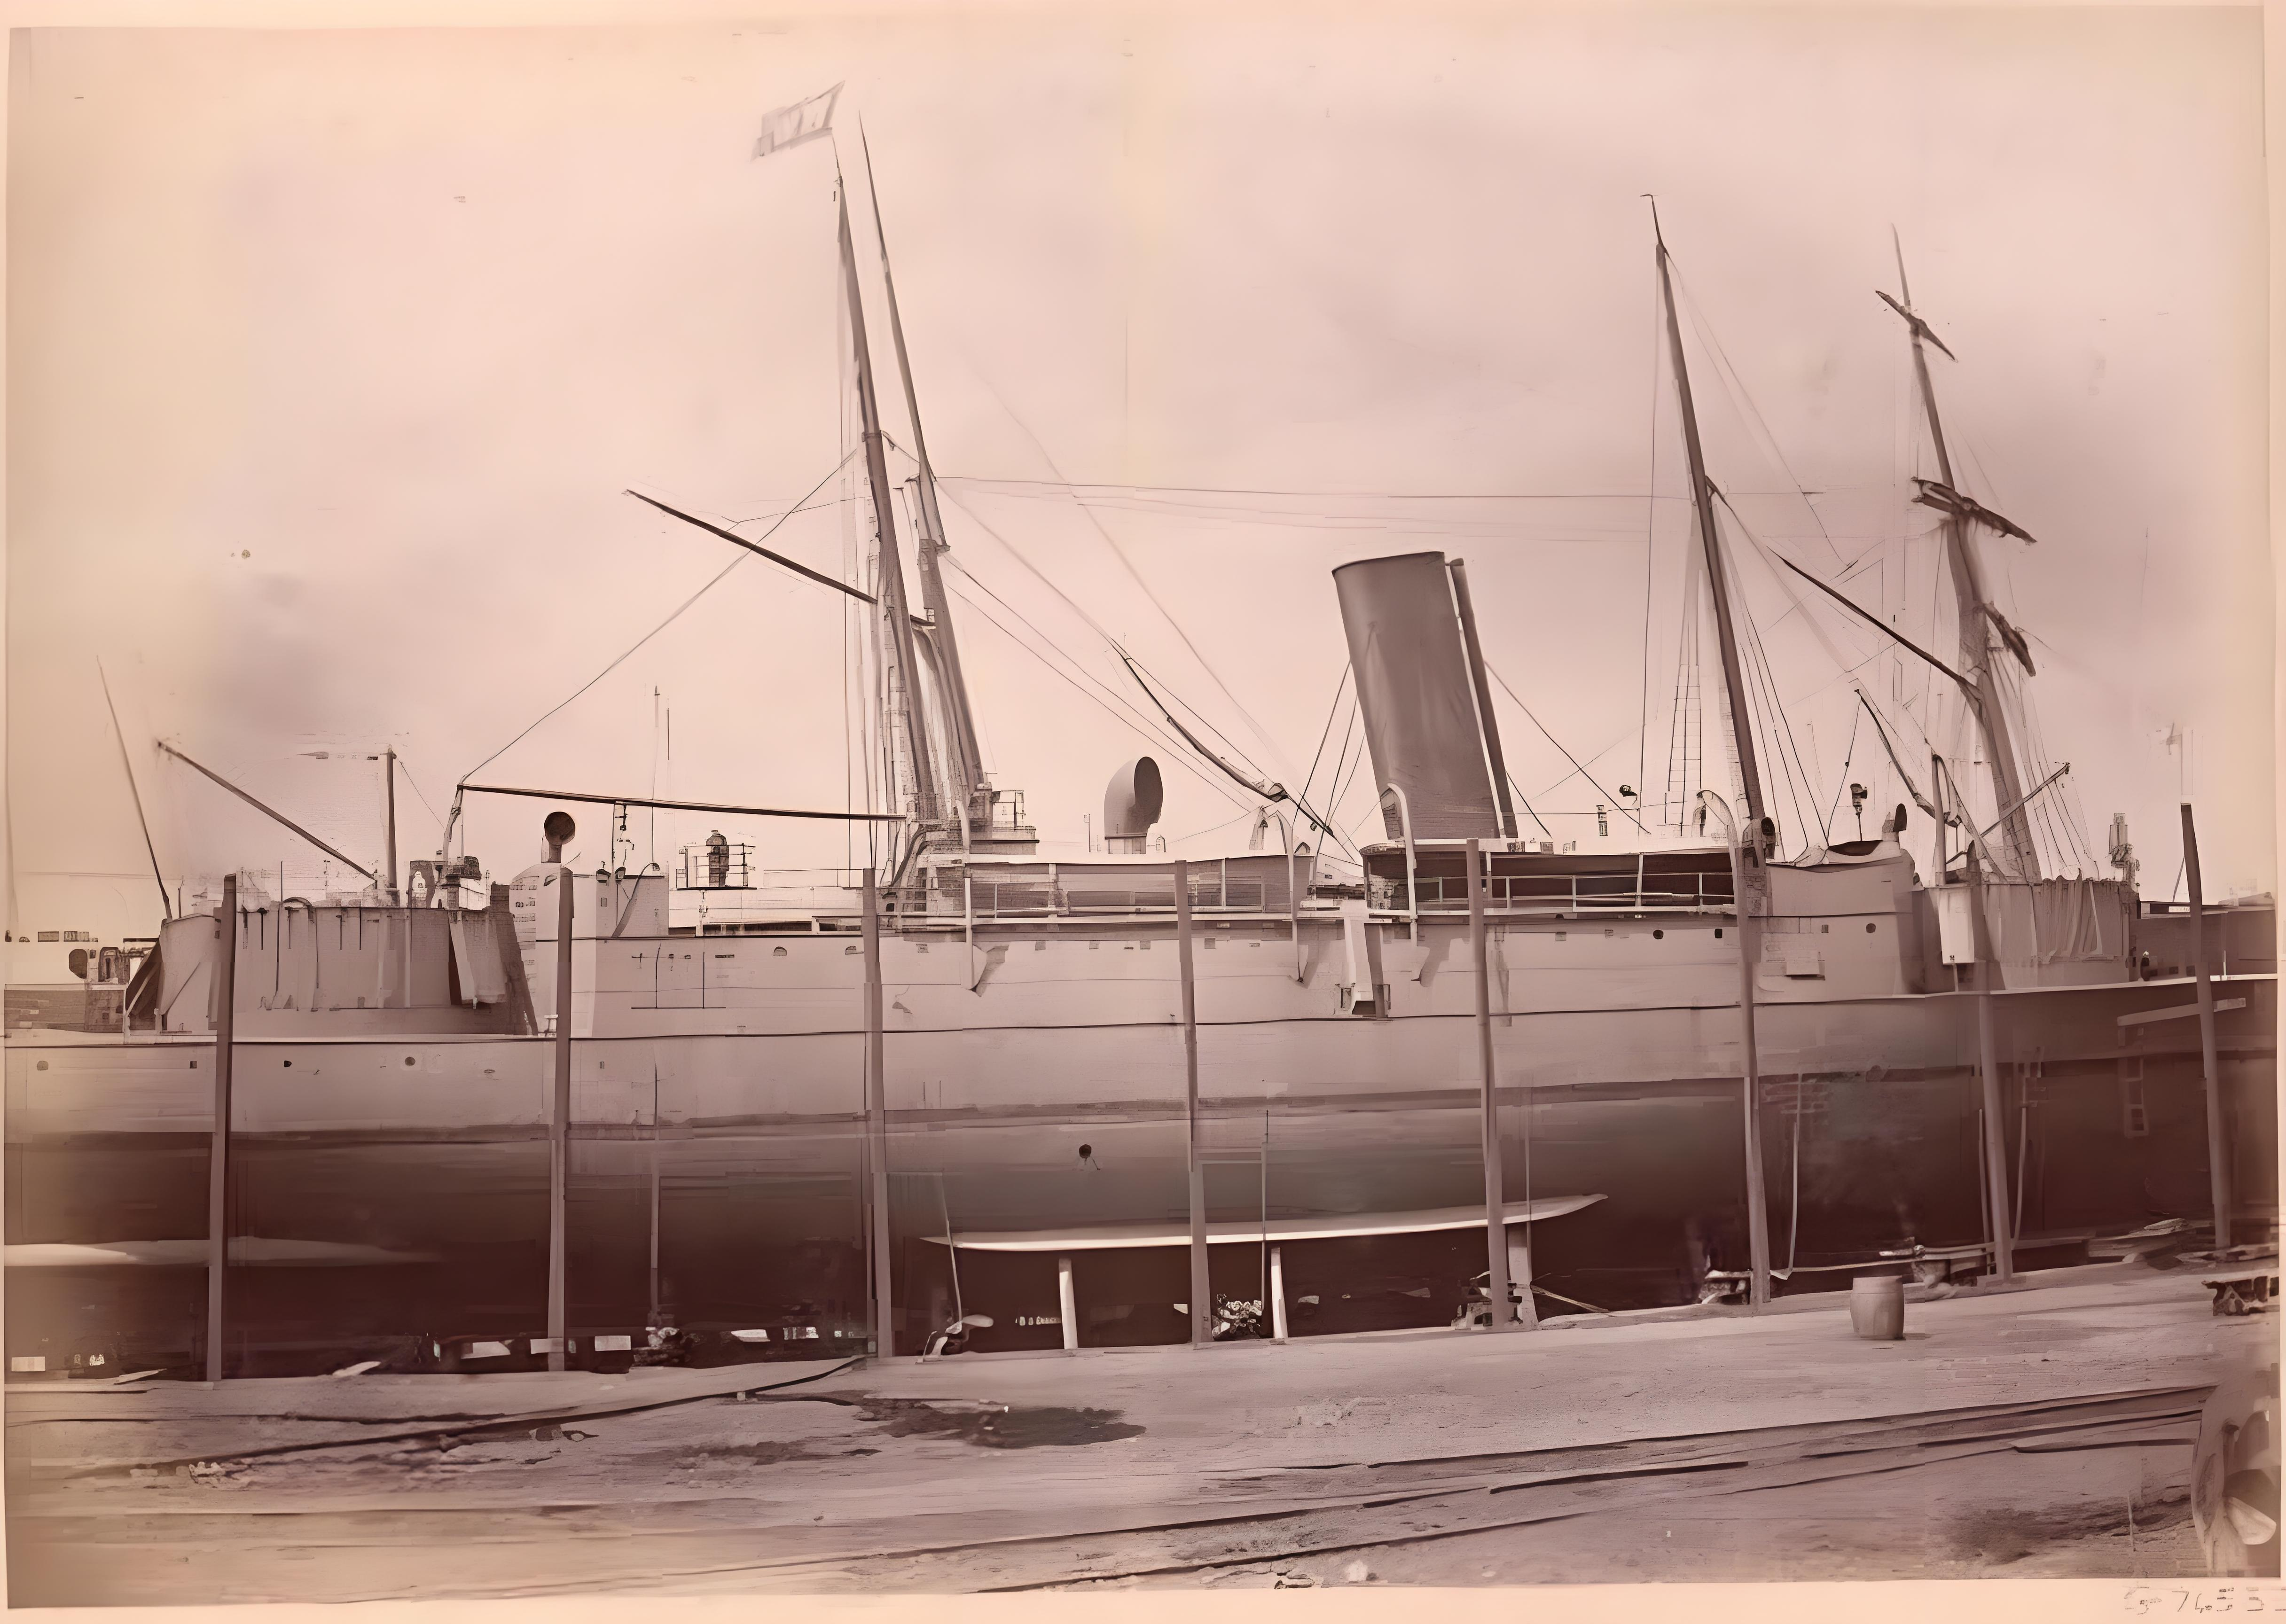
\includegraphics[width=1\linewidth]{Images/24}
	\caption{在米切尔船厂船台上等待下水的“白羊座”“超勇”}
	\label{fig:1}
\end{figure}

\begin{figure}[htbp]
	\centering
	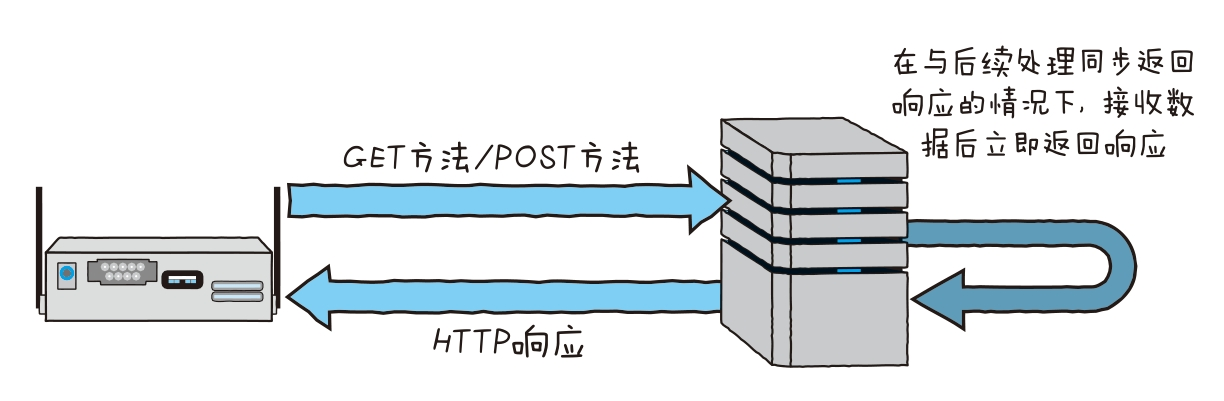
\includegraphics[width=1\linewidth]{Images/25}
	\caption{“超勇”级军舰所用的霍索恩卧式蒸汽机}
	\label{fig:1}
\end{figure}

“超勇”级军舰的舰体为金属结构,舰壳材料主要采用的是3/4英寸厚的钢板,另外在水线下3.5英尺处有一段简化的装甲甲板,保护着机舱和弹药库等重要部位,但这层装甲甲板厚度仅为3/8英寸,只能给水兵们一些心理安慰而已,并无太多实际价值。除此外,“超勇”级再无附加装甲,实际上属于无防护巡洋舰,这样设计的主要目的是出于减轻军舰的吨位、提高航速,以及降低成本等考虑。为增加军舰的生存力,伦道尔在军舰舷侧和机舱上方设置了多个煤舱,寄希望依靠煤堆来提供一些防护。

因为自身防护能力薄弱,而作战的主要手段又是极为冒险的撞击战术,“超勇”
级军舰外形设计上别具特色。除双桅、单烟囱外,水线以上的舰体非常简洁、低矮,如此既使对方难以瞄准,逃避敌方火力的打击,同时又能尽量隐蔽自己,不被敌方发现,以发挥撞击战术突然性的特点,其设计思路非常类似今天的隐形军舰。但由之却造成了适航性差的恶果,该级军舰干舷极低,即使在风平浪静的情况下高速航行,艏艉主甲板也可能被海水淹没,恶劣海况下的情况可想而知。为此,“超勇”级军舰艏艉的主甲板不作为水兵工作的主区域,没有敷设柚木甲板,通常布置在主甲板的吊锚杆被安排到了前后主炮塔顶上,这样起锚作业时,水兵的工作环境相对安全,然而吊锚杆位置过高,尽管按照赫德的要求安装了蒸汽起锚机,仍不可避免会影响起锚作业的时间。

“超勇”级军舰指挥系统的布置较有特色,在前主炮房后部、烟囱后部两处各设有一座装甲司令塔,但装甲厚度仅为5/8英寸,前主炮房后部的装甲司令塔顶上安装有1座探照灯,烟囱后部的装甲司令塔顶部则设有露天飞桥。此外,在后主炮附近还有一个备用的露天指挥台,安装有1具标准罗经。

沿袭蚊子船小船架大炮的设计思路,伦道尔给小小的“超勇”级军舰安排了2门大口径后膛火炮。这种由阿姆斯特朗公司生产的火炮,可能是MKI型,口径10英寸,身管26倍径,炮弹重400磅,每门炮备弹100发,正常情况下最大射击仰角10度,最大射击俯角3度,有效射程8000米,在极限射击仰角15度时,射程可达12000米,威力在当时可谓相当惊人,被认为是1881年代威力最大的火炮,3000米距离上使用实心弹可以射穿14英寸厚的钢板,这可能是伦道尔向金登干许诺这种军舰可以战胜铁甲舰的信心所在。由于这型火炮属于从地井炮发展而来的原始速射炮,带有原始的液压复进装置,因此射速较传统的架退式后膛炮为快,为2.5分钟1发。因为该型巡洋舰的吨位较小,没有采用笨重的船面旋台式炮塔,而是将2门火炮分装在军舰艏艉的露炮塔里,火炮采用水压动力转动,每门炮配备10名炮手。为给炮手提供一个相对较好的工作环境,以免风浪的干扰和保持舰体外观连贯避免突兀以增加隐蔽性,在露炮塔外安装了一个固定不能转动的炮廓,炮廓钢板的厚度仅有3/8英寸,分别在火炮的正前方和两侧开有较大的炮门,主炮在正前方可以获得44度的射角,在左右两侧分别获得70度的射角。由于“超勇”级军舰的干舷很低,高速航行时甲板容易上浪,未免海水灌入炮台内,炮门上均装有挡板,平时关闭,作战时向上掀放到炮台顶上。

\begin{figure}[htbp]
	\centering
	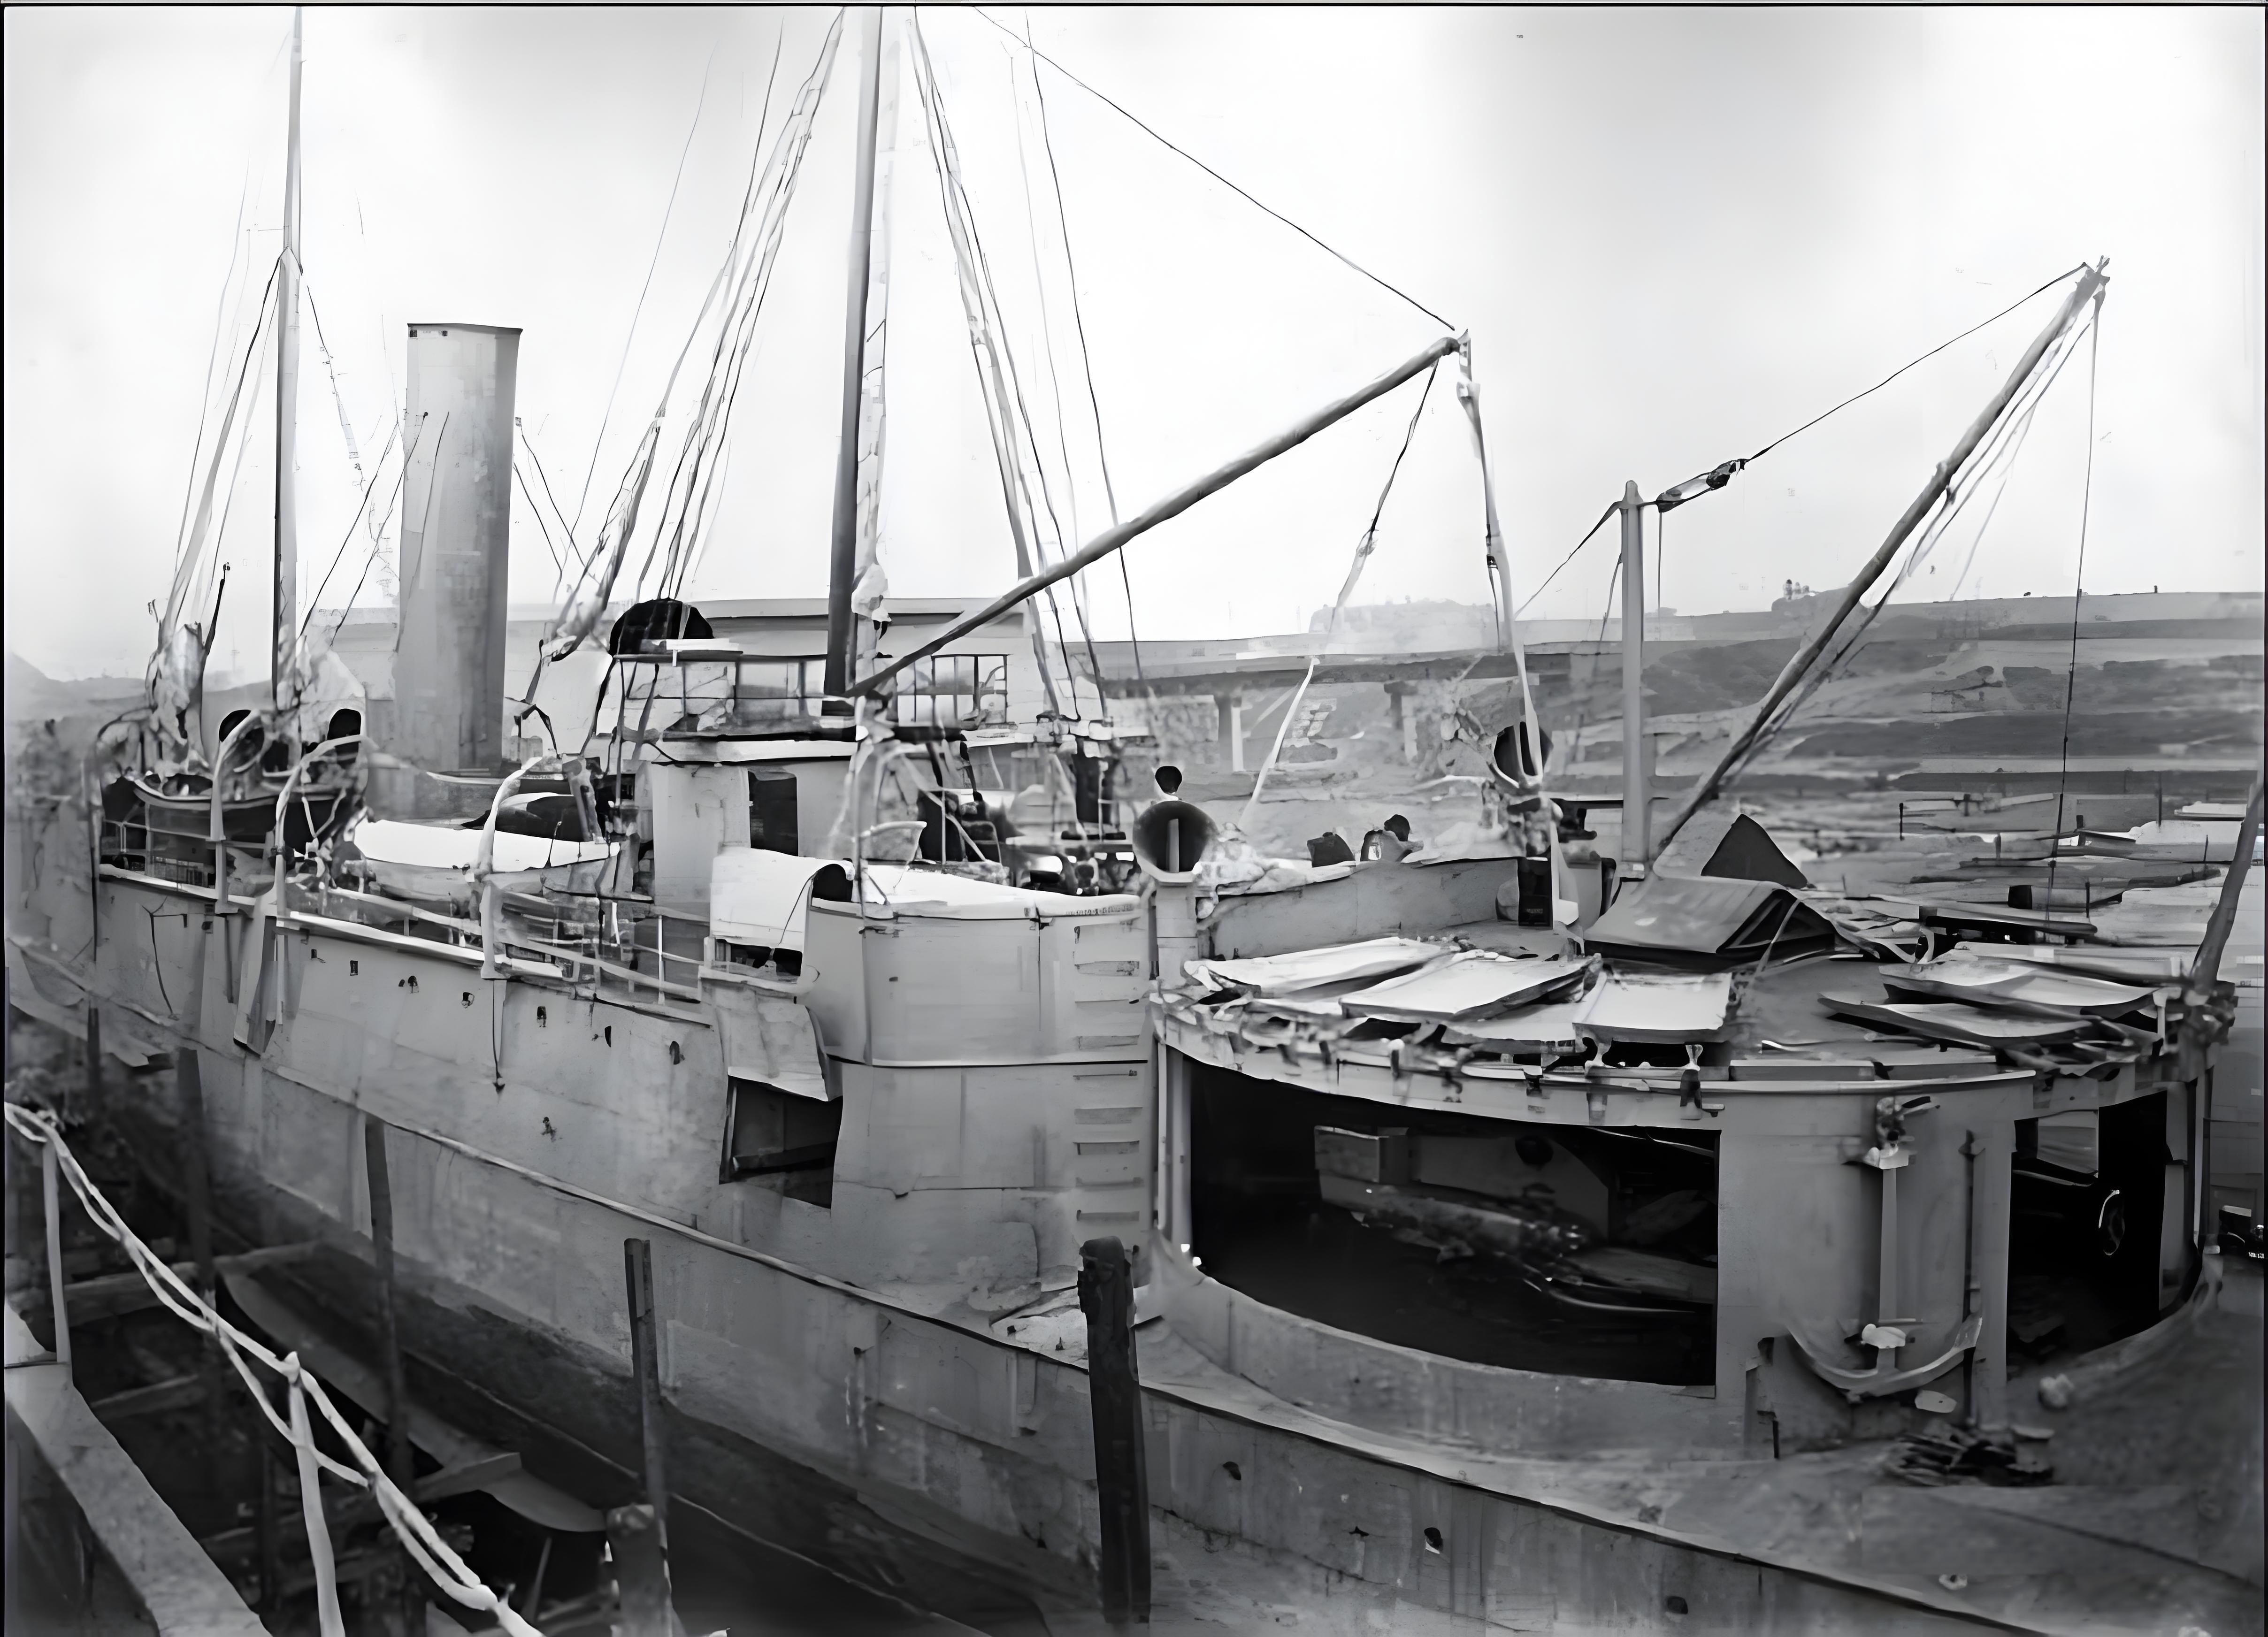
\includegraphics[width=1\linewidth]{Images/26}
	\caption{在左舷后方拍摄的“超勇”级军舰照片,可以看到折叠安放的炮门挡板。}
	\label{fig:1}
\end{figure}

符合当时军舰的设计标准,“超勇”级军舰在主炮之外装备了大量中小口径火炮,用来填补舰上的火力真空。其中,4门阿姆斯特朗公司生产的4.7英寸口径火炮,被安装在上层建筑内的4个拐角上,通过舱壁上的炮门向外射击,射界60度,这种火炮同样属于由地井炮发展而来的原始速射炮,身管长22倍口径,每门炮备弹200发,弹重40磅。和主炮一样,为防止海水灌入,4.7英寸炮的炮门上也使用了挡板,作战时才向上打开。\footnote{Richard N J Wright: The Chinese Steam Navy, Chatham Publishing 2000, p49.}

\begin{figure}[htbp]
	\centering
	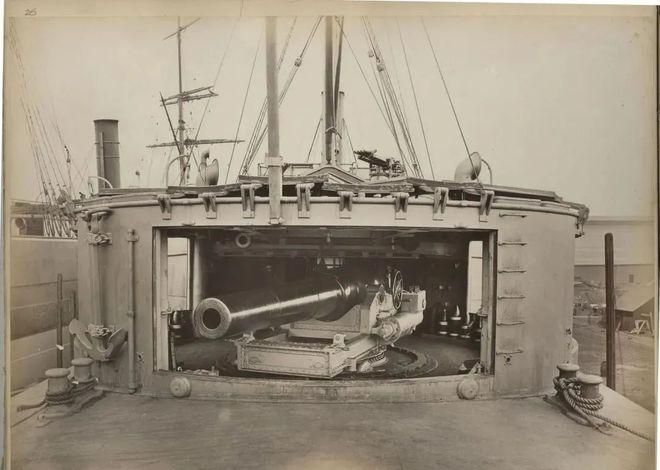
\includegraphics[width=1\linewidth]{Images/27}
	\caption{“超勇”级舰艉炮房里的10英寸口径后主炮。}
	\label{fig:1}
\end{figure}

“超勇”级后主炮附近还安装有2门诺典费尔德式(Nordenfelt,又译为诺登飞)4管机关炮,中国史料称为四门神机连珠炮。这种火炮是当时世界与哈乞开司、格林等齐名的优秀多管机关炮,原理是将多根炮管平行排列,通过转动把手,使各个炮管后的枪机依序击发,从而实现高速射击。火炮口径25毫米,炮身长965毫米,炮身重193公斤,炮架重117公斤,射速每分钟350发,射程2000米,274米距离上可击穿24毫米厚钢板。此外,舰上的小口径炮还有4门10管格林机关炮。

\begin{figure}[htbp]
	\centering
	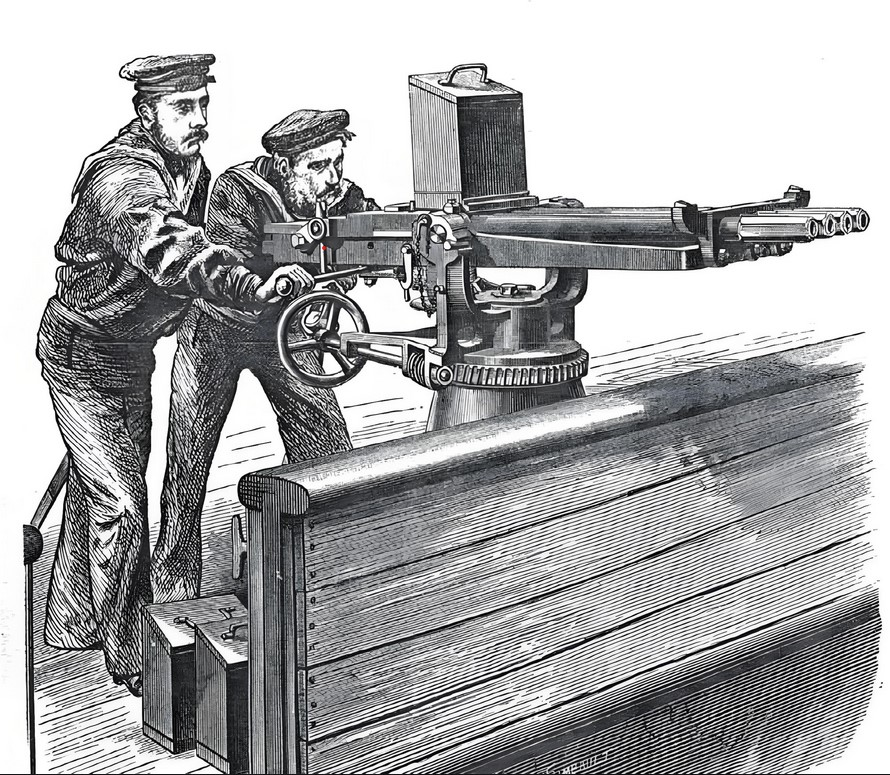
\includegraphics[width=1\linewidth]{Images/28}
	\caption{表现英国水兵操作诺典费尔德机关炮情景的铜版画。}
	\label{fig:1}
\end{figure}

作为撞击巡洋舰,“超勇”级军舰必不可少的武器是撞角,据西文档案记载,撞角位于舰艏水线下11英尺处。但在今天掌握的最早的一套“超勇”级军舰图纸上,却找不到一点有撞角的迹象,据推测是因为撞角的设置增大了舰艏的兴波阻力,航速受到影响,所以被迫改为垂直艏,保持军舰在平时航行时的流线完好。

最后,“超勇”级军舰还有一项特殊的武器——鱼雷兵器。正是这种武器,一度让赫德、金登干、伦道尔伤透了脑筋,更一再引起李鸿章的不快乃至震怒。事情要从金登干最早推荐军舰的那封信说起,当时为了吸引客户,伦道尔承诺可以提供航速不低于16节的舰载鱼雷艇,一贯用词夸张的赫德、金登干便添油加醋汇报给了李鸿章。但在建造过程中发现,排水量1380吨的巡洋舰上,搭载的小艇长度最多不能超过15英尺,如果再大一些,巡洋舰就会缺少足够的挂载空间和搭载所需的剩余浮力,“超勇”级巡洋舰的干舷本来就很低,配备的大炮又很重,而且起吊放下鱼雷艇的作业也很困难。所以,舰载鱼雷艇的大小是受到严格限制的,可在15英尺的小艇上又能够放得下多大的动力设备以保证16节的航速,更何况还要装上鱼雷发射管和至少1条鱼雷。由此,给“超勇”配装舰载鱼雷艇成了不可能完成的任务。

\begin{figure}[htbp]
	\centering
	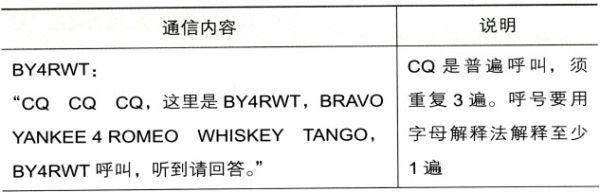
\includegraphics[width=1\linewidth]{Images/29}
	\caption{“超勇”级军舰主甲板特写,舷边可见搭载的汽艇。}
	\label{fig:1}
\end{figure}

\begin{figure}[htbp]
	\centering
	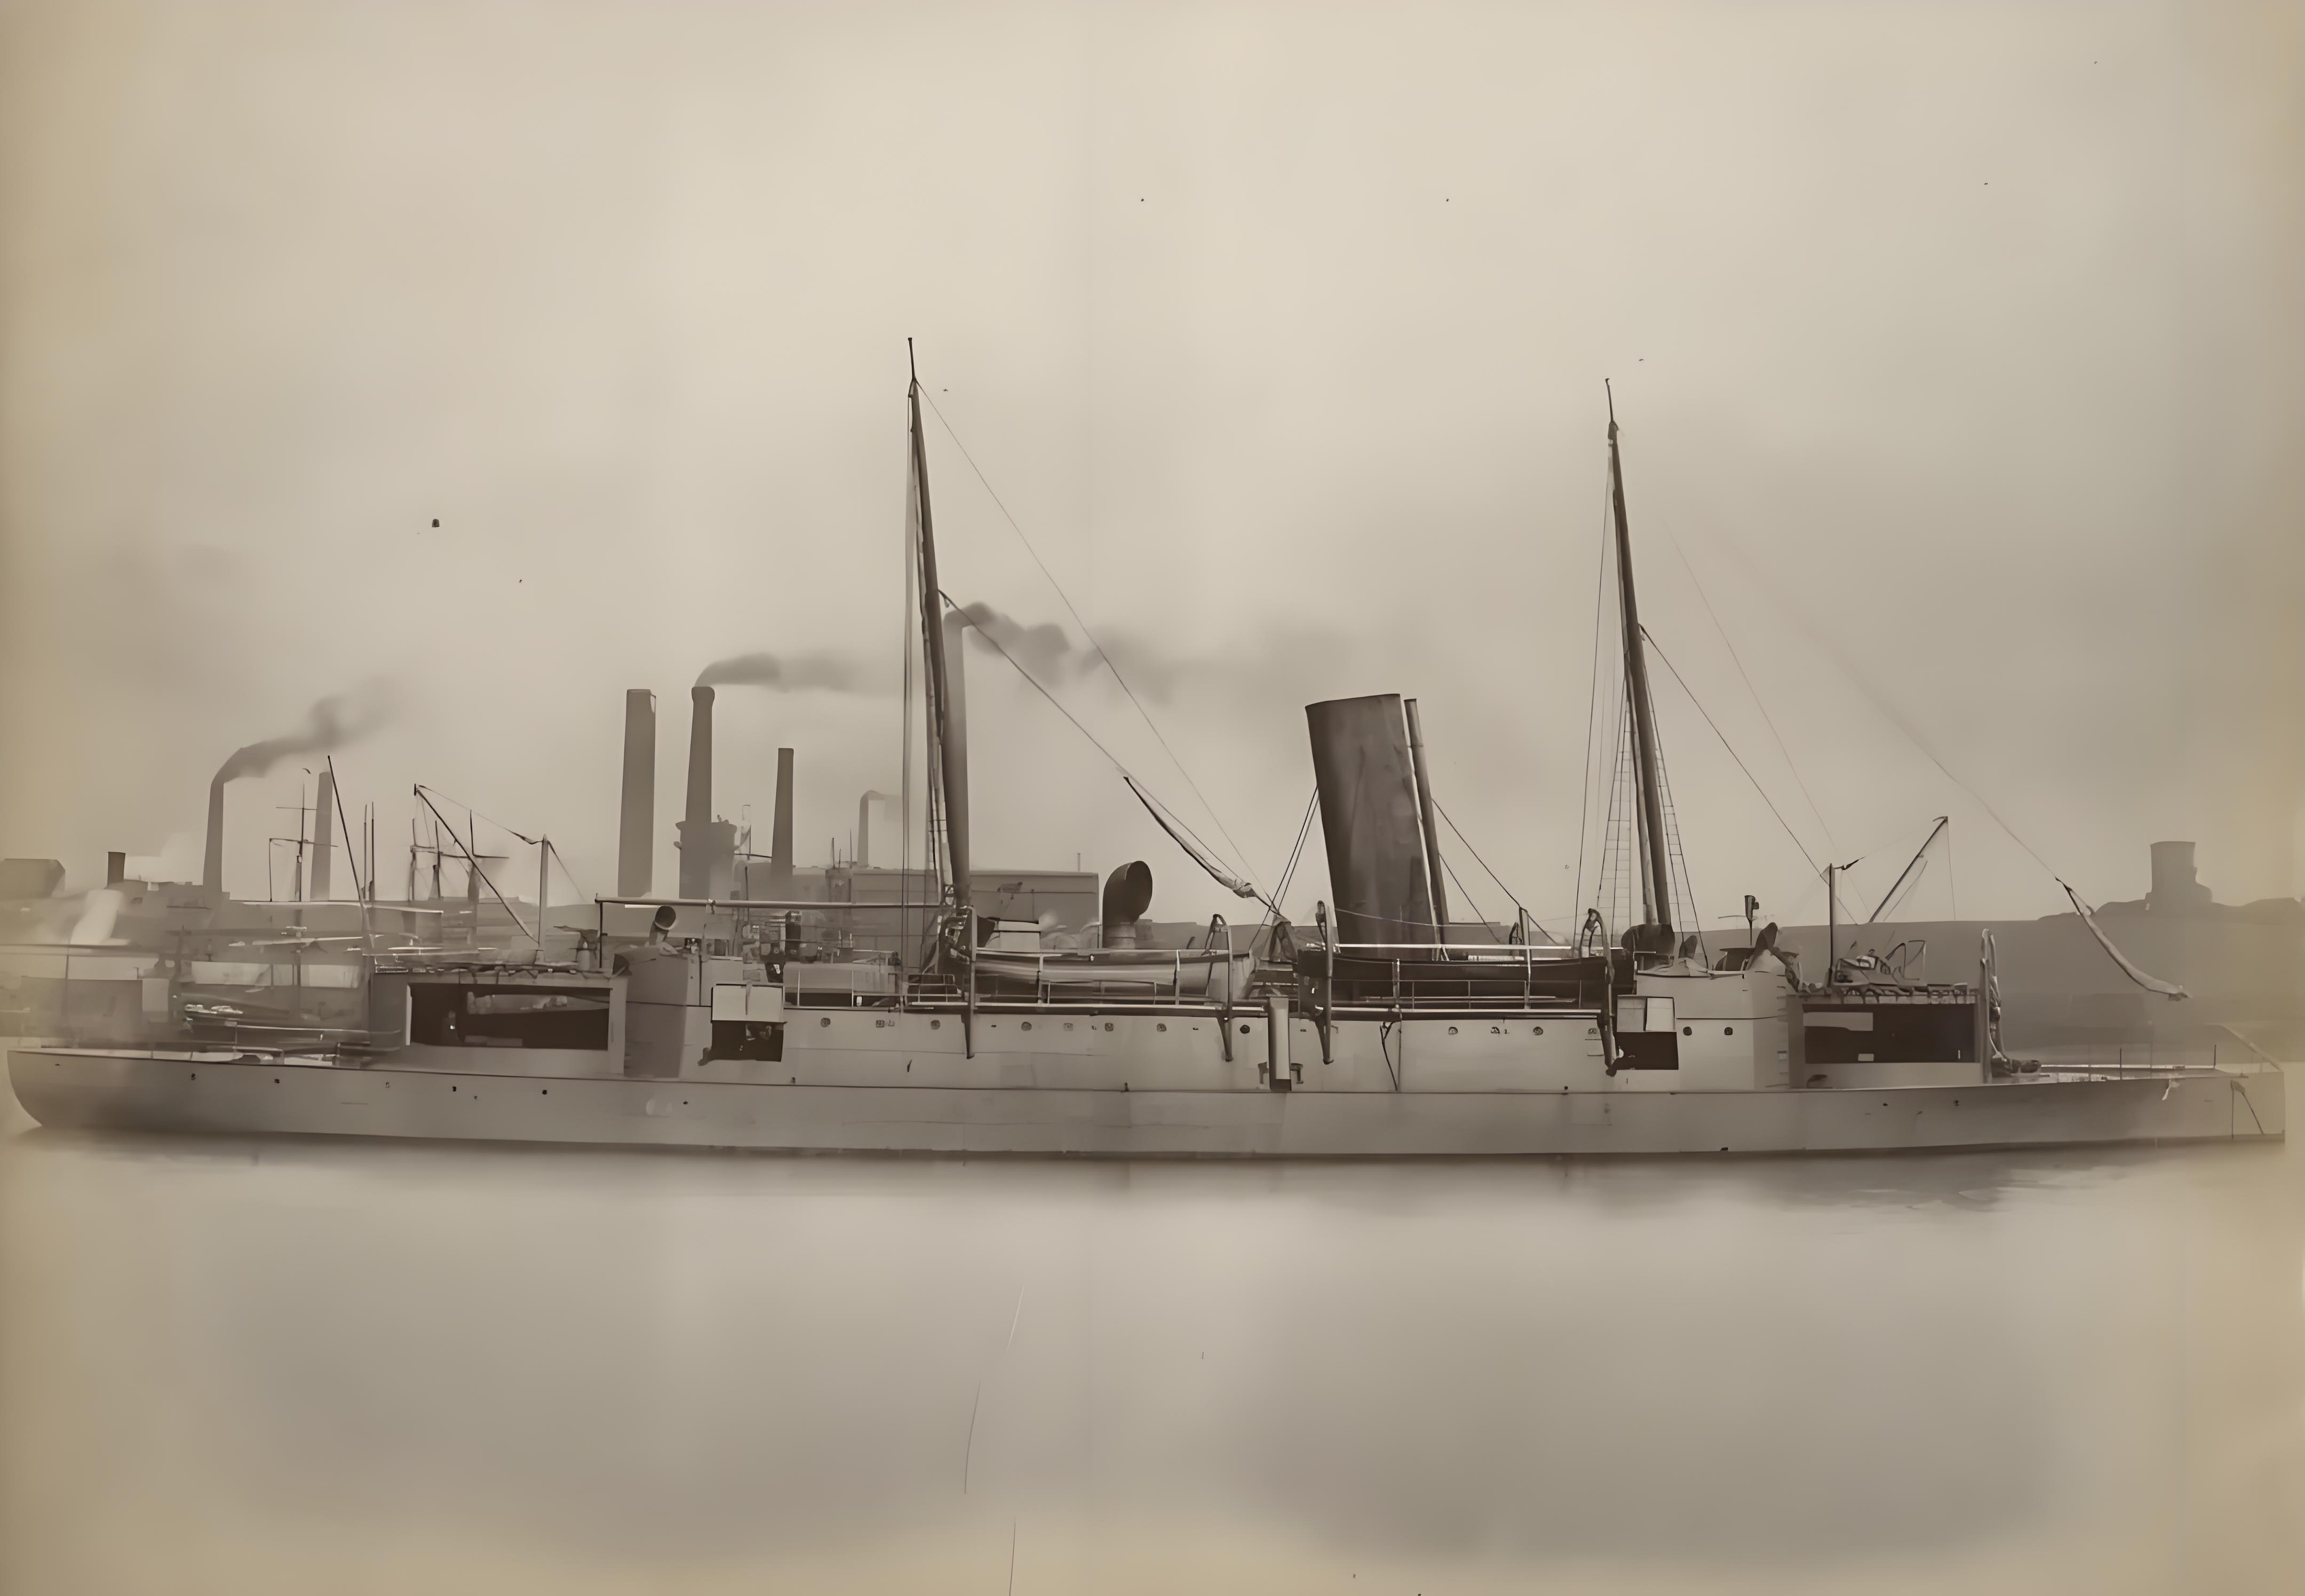
\includegraphics[width=1\linewidth]{Images/30}
	\caption{竣工后的“超勇”级巡洋舰。}
	\label{fig:1}
\end{figure}

\begin{figure}[htbp]
	\centering
	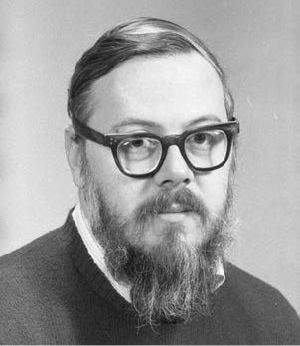
\includegraphics[width=1\linewidth]{Images/31}
	\caption{“超勇”级巡洋舰关闭所有炮门时的状态。}
	\label{fig:1}
\end{figure}

赫德在中国海军建设领域的好运似乎快用尽了,令他意外和难堪的是,后来了解到,李鸿章当初决策购买巡洋舰的一条重要原因,居然是因为看中了该舰有舰载鱼雷艇。尽管伦道尔用充足的理由告诉金登干为什么不能搭载鱼雷艇,金登干也原原本本转述和说服了赫德,但是赫德实在没有勇气向李鸿章启齿,去告诉这位主持中国海军建设的实力人物,他所一心期望得到的鱼雷艇是不可能的。后果实在难以设想,久居中国,深知清王朝官场规则的赫德于是大玩太极推手,不断向金登干施压,要金登干自己向李鸿章解释。被逼无奈,金登干和伦道尔想出个有些儿戏的解决办法,提出用能装备杆雷的汽艇(杆雷艇)替代舰载鱼雷艇,耍起了文字游戏。

事已至此,加上当时出现了俄国扬言要派舰队进攻渤海湾的险恶形势,为不影响2艘巡洋舰的交货,李鸿章只好强压怒火接受。之前因相信赫德的推荐而购买蚊子船已经备受同僚攻击,现在新巡洋舰上又出现这种事情,李鸿章对赫德彻底失去了信心,认识到赫德、金登干都不过是夸夸其谈的海军外行而已。赫德很快感受到了后果的严重性,做了多年的总海防司美梦被李鸿章一手击碎,此后中国购买新军舰也不再通过赫德了。李鸿章心里对赫德的恼火,最终通过他的得力幕僚薛福成淋漓尽致地表达了出来:“……赫德为人,阴鸷而专权,怙势而自尊,虽食厚禄,受高职,其意仍内西人而外中国……”\footnote{《上李伯相论赫德不宜总司海防书》,见中国近代思想家文库《薛福成卷》,北京:中国人民大学出版社2014年版。}鸦片战争时期,那种中国官员任洋人欺凌的时代确实过去了。

经过如此一番波折,“超勇”级军舰上的舰载鱼雷艇于是缩水成了杆雷艇。在鱼雷诞生之前,各主要海军国家大都装备了水雷,在美国南北战争中水雷曾大显神威,受到各国海军界的重视。但水雷毕竟是固定不动的,只能被动防守,无法主动攻敌。为解决这一矛盾,英国人想出了拖雷的办法,即用钢索把水雷拖曳在舰艇的后面,或呈30度角拖曳在两侧,攻击敌舰时,先向目标高速驶去,然后突然转弯把“辫子”一甩,使水雷撞上敌舰从而达到攻击效果。然而这种做法过于冒险,此后英国人在机动汽艇(即木舢板上加装小锅炉,中国称为火轮舢板。出于耐脏等目的,汽艇艇身大都油漆黑色,艇底因为包裹铜皮,一般为铜本色)上进行改造,加装一根8、9米长的铁杆,首段携带水雷,平时铁杆收回在艇内,等接近敌舰时突然伸出碰撞敌舰引爆,这即是杆雷艇。“超勇”级军舰装备的杆雷艇回国后未见使用,估计更多时候是拆掉铁杆,直接用作交通艇。

在世界军舰发展史上占有里程碑式地位的“超勇”级撞击巡洋舰,建成当时是世界最新式的军舰,作为体现新技术、新思想的概念舰,本身不可避免地会存在诸多不足之处,诸如适航性差、防护薄弱、“一遇风浪则炮难取准,偶受小炮即船已洞穿”,都是“超勇”级军舰不容回避的缺陷,但这级军舰开辟了舰船领域的一个新类别,而且对英国乃至世界巡洋舰的设计产生了深远的影响。19世纪后期英国建造的智利Esmeralda号、日本“浪速”级、意大利Giovanni Bausan级巡洋舰上,都能找到阿姆斯特朗公司第一型出口巡洋舰——“超勇”级的影子。至于中国一些论著中,以“超勇”级军舰装甲单薄而认为该型舰质量低劣的评论,与批判水炮台型的蚊子船不能出大海作战一样,都是属于典型的缺乏十九世纪海军常识的局外之谈。而以当时舰龄已逾十载的“超勇”,在1894年黄海大战中的表现不佳为例,批评该型军舰质量不佳,更属没有时间概念之谈。

\section{远航英伦}

1880年12月6日,天津西沽热闹非凡,停泊在此的各国军舰均悬挂满旗,鸣放礼炮,向正在缓缓出港的招商局“丰顺”号轮船致敬,中国海军历史上第一次大规模赴外接舰团启程了。此前,中国在外购买的军舰,都是花重金雇佣国外技术人员驾驶回华,为培育、锻炼自己的海军人才,也为节省经费起见,李鸿章经与赫德反复争辩,最终作出决定,派出中国自己的海军官兵前往英国,接收2艘“超勇”级军舰。

经清廷允准,北洋海防督操、记名提督丁汝昌率管带林泰曾、副管带邓世昌,大副蓝建枢、李和,二副杨用霖,正管轮黎星桥、陈学书,副管轮王齐辰、陆保,管队袁培英、何桂福,军医江永、杨星源,总教习葛雷森(Glayson),管驾章斯敦(Johnstone),随行的文案池仲祐等20人,以及经过严格挑选的来自山东荣成、文登、登州(今蓬莱)等地,原属旧式登荣水师的224名舵工、水勇、夫役组成接舰部队。

丁汝昌,字雨亭,又作禹廷,安徽庐江人。淮军铭军出身,因为在镇压太平天国及捻军的战争中作战勇猛,升至铭右军统领。1879年被李鸿章调入北洋海防差遣,担任轮船督操,从此开始了他的蓝色生涯。尽管不是海军科班,但丁汝昌以其特有的尽职精神和谦虚的态度,在能力所及范围内尽力学习、汲取海军知识,又因为人和蔼,关心部下,深得北洋全军拥戴,当时西文报章称其为令人尊敬的绅士。李鸿章此次派丁汝昌及众多海军官兵远赴英伦,别有深意,潜台词是期望海军人才能尽快成长起来。

\begin{figure}[htbp]
	\centering
	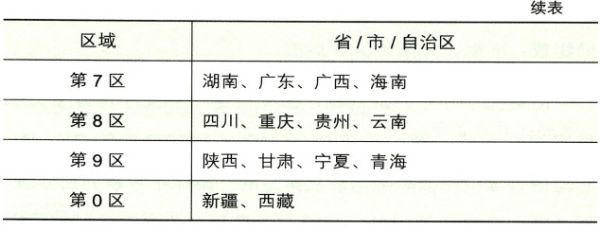
\includegraphics[width=1\linewidth]{Images/32}
	\caption{接舰期间,丁汝昌在英国纽卡斯尔门德尔松照相馆拍摄的肖像照。}
	\label{fig:1}
\end{figure}

12月10日拂晓,接舰部队抵达上海,借住在南洋水师的“驭远”号军舰。当日下午,开始定制各类的军服以及旗帜,总价5000银洋,为保证不延误工期,丁汝昌要求供货商立下军令状。同时又将接舰部队划成两部,分由林泰曾、杨用霖及章斯敦、邓世昌管理、操练。23日,丁汝昌偕同葛雷森等先期乘法国商船赴英,计划等验收诸事完成后,再招大部队前往,以便节省经费,这位中国海军未来的统帅开始了他职业生涯中第一次远航。留在上海的部队及一应公事,由林泰曾会同章斯顿管理。

来年的2月14日,招商局商轮“海琛”号改装一新,原有的货舱改制成住舱,可以安排300架床位。是日,接舰部队全部移居“海琛”轮,为解决“海琛”轮舵工、水手、升火等岗位人手短缺的困难,林泰曾又在沪临时添招了40人,接舰部队的水兵数量由此升为264名。20日,丁汝昌从英国发来电报,命令接舰部队出发。

2月27日,天气阴,气温华氏40度(约为摄氏4度)。上午9时整,吴淞炮台鸣放大炮,声势震天,口内的南洋水师各军舰“皆升旗发炮”,这块曾洒下江南提督陈化成将军一腔热血的土地,见证了中国海军的再次起步,寒风料峭中,“海琛”轮满载中国海军官兵拔锚远赴英伦。

经过近2个月的漫长航行,4月22日入夜,“海琛”轮在雨雪纷飞中进入英国伦敦界,望着工业文明下,“岸边灯光燎亮,联络数里”的独特景象,第一次到达大英帝国的中国海军官兵们心潮澎湃,思绪万千,这是祖先们无法想像的事情。船上的官兵们不知道的是,当天下午,他们的提督丁汝昌,在金登干陪同下拜访了英国海军部,和英国海军提督凯古柏、海军部总工程师斯图尔特、军舰设计师巴纳贝进行了长时间会谈,并参观了英国最新式战舰的模型和图纸,进行了中英两国高级海军军官的第一次历史性的交流。\footnote{《中国海关密档》2,北京:中华书局1995年版,第542页。}在此之前,先期到达的丁汝昌一行已参观了阿姆斯特朗公司,以及建造中的“超勇”、“扬威”,丁提督还兴致勃勃地亲自监督“超勇”、“扬威”舰试炮。在伦敦期间,丁汝昌受到维多利亚女王接见,并在中国使馆配合下,在英国海军界开展了一系列公关活动,好评如潮。

\begin{figure}[htbp]
	\centering
	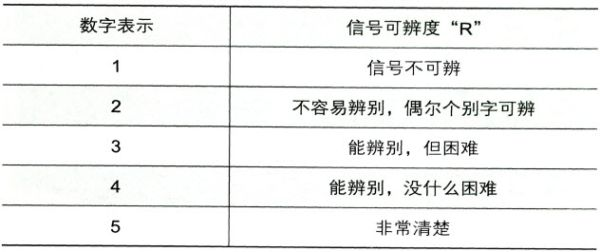
\includegraphics[width=1\linewidth]{Images/33}
	\caption{英国报纸上刊载的铜版画:丁汝昌参观英国海军医院。}
	\label{fig:1}
\end{figure}

4月24日清晨,“海琛”轮进入泰恩河,在英国引水员导航下,到劳沃克船厂,官兵们见到了建造中的“超勇”、“扬威”。次日,从伦敦赶来的丁汝昌登上“海琛”,慰问之余,要求全体官兵“早晚站班点名”、“各执事按日办公如兵船”\footnote{池仲祐:《西行日记》,北京:商务印书馆1908年版,卷上,第13页。}。4月30日,“海琛”轮抵达纽卡斯尔,驻泊于阿姆斯特朗公司的所在地埃尔斯维克(Elswick),一路上“夹岸土人观者如堵”,迎风招展的龙旗,装束奇特的水兵,在英国举国上下引起了轰动,此时距圆明园的大火熄灭仅过了20余年,中国已经从痛苦的深渊中挣脱出来,年轻的中国海军第一次自信地站到了世界舞台上,清楚地传达着一个信息,这是一个不甘沉沦的民族!

5月5日,“海琛”轮上陆续有中国水兵放假上岸,“沿途土民随观者甚众”。8日是礼拜天,气氛到了高潮,“土人集岸边观船者约千人,男女上船观者联络不绝”\footnote{池仲祐:《西行日记》,北京:商务印书馆1908年版,卷上,第14页。},许多通晓英语的中国官兵很快交上了英国朋友。海军传统深厚的英国人民,对远道而来的东方古国的年轻海军表现出异常的热情,登船参观者逐日增加,“士女来船观者日以加,甚有不相识而以物及影(照片)相赠者”。为表示欢迎,纽卡斯尔市市长特别邀请全体中国官兵观看马戏表演,整队坐车前往剧场的路上,“沿途观者肩摩肘掣,拥挤不开,土人各以手挥帽作礼”。期间时值火车发明者斯蒂文森(Georeg Stenphenson)百岁寿诞,纽卡斯尔市政府举行大型宴会,丁汝昌、林泰曾应邀与当地官员、士绅、名人等400余人出席。席间纽卡斯尔市长和阿姆斯特朗起身祝酒,表达对中国和中国海军的良好感情,丁汝昌与林泰曾亦致祝酒词。林泰曾用一口流利的英语发表的致辞:“我中国提督与在座诸君致谢,非独谢今日之宴也,盖谓中国员弁勇丁到此以来,受诸公及本地民人之款待为已优矣。但愿英与中国永相和睦,无忘旧好,且斯蒂文森百年寿庆,我中国官员得附盛宴,何胜荣幸,愿斯蒂文森子孙世享其泽。夫斯蒂文森创立火轮车,美利几遍各国,我中国他日用之大获其利,则中国之幸,亦诸君之幸也。\footnote{池仲祐:《西行日记》,北京:商务印书馆1908年版,卷上,第28--29页。}”当即引起轰动,第二天当地的报纸予以全文转载。

\section{英国上空的黄龙旗}

春天如约而至的中国官兵,并没有立即获得他们的军舰。因为遇到材料涨价、设计修改,以及罢工、鱼雷艇问题等一系列麻烦事,尽管米切尔船厂都想出了要把智利船上的部件拆给中国军舰用的主意,“超勇”、“扬威”的完工日期还是受到了影响。而且竣工后,2艘军舰还需要进行航试,但持续的恶劣天气让航试一再延期,合同约定的春天交船日期早已过去。远在天津的李鸿章对英方没效率的工作越发不满,以致勃然大怒。整个1881年的6、7月间,赫德发往英国的电报和信件,出现频率最高的词就是巡洋舰,“巡洋舰何时起航?”、“巡洋舰误期使李震怒,日益不耐烦。请立即把船派出,如果再拖延,恐将下令不予提货!”、“巡洋舰是否永不起航?!”\footnote{《赫致金第31号》《赫致金第33号》《赫致金第34号》,《中国海关密档》8,北京:中华书局1995年版,第249、250页。}

这段时间估计是金登干生命中最难熬的日子,不仅要应对大海那边赫德的催促,解释、平息赫德和李鸿章的怒气,还要面对眼前丁汝昌的脸色,以及阿姆斯特朗公司和米切尔船厂的抱怨。谢天谢地,总算1881年的7月14、15日来到了,星期四和星期五这两天里,在中国海军军官的监督下,“超勇”和“扬威”分别进行了航速和射击测试,结果让所有人松了口气。离岸不远的海面上,2艘军舰在距离10.75海里的两点间各自跑了个来回,“超勇”测得轮机功率2800马力,航速16.5节,“扬威”虽然在测试途中为避开误闯进来的渔船,而一度偏离航线,然而也得到了2700马力和16节的好成绩,2舰均达到设计要求。\footnote{《中国海关密档》2,北京:中华书局1995年版,第598页。}

27日,两艘军舰完成了最后的一点工作,补充了短缺的补给品,驶入母厂进行最后一次检修,更换螺旋桨、清洗船底、油漆船身。随后8月2日,中国接舰部队正式登舰,林泰曾、杨用霖等率领的一部接收“超勇”号,章斯敦、邓世昌率领的部队接收“扬威”号,丁汝昌及总教习葛雷森以“超勇”号为旗舰。\footnote{池仲祐:《西行日记》,北京:商务印书馆1908年版,卷下,第9页。}

第二天凌晨,洋务运动领导人物曾国藩的长子,中国驻英公使曾纪泽在船政留学生洋监督日意格等的陪同下,从伦敦乘火车抵达纽卡斯尔。经过短暂休息,下午2时,鼓乐声中,曾纪泽亲手将三角龙旗升上“超勇”、“扬威”的旗杆,二舰礼炮齐鸣,在场的中国官兵胸中激荡着冲天豪情,深切体会到了国家的尊严和强国的荣耀,旁观的英国群众则纷纷欢呼祝贺,中国龙旗第一次在英国本土骄傲地飘扬。随即,2艘高悬龙旗的军舰又开出港口测试大炮和航速,傍晚折返加罗斯拉克(Jarow Slake)寄泊。英国海军部的总工程师海军上将豪斯顿·斯图尔特爵士、赖特以及费雷德里克·拉姆斯威尔爵士都出席了升旗仪式,并详细检查了2艘军舰,对军舰表示了高度赞扬。在这临别时刻,纽卡斯尔市长发来一封信:“纽卡斯尔市长谨向丁提督致敬,并通知他,在今天举行的市议会上,一致决定在他离开泰恩河之前向他献一份祝辞。丁提督如能见告接受这项祝辞何时方便,在他的船上抑或在市政厅举行,本市长将不胜感激。”\footnote{《中国海关密档》2,北京:中华书局1995年版,第604页。}

\begin{figure}[htbp]
	\centering
	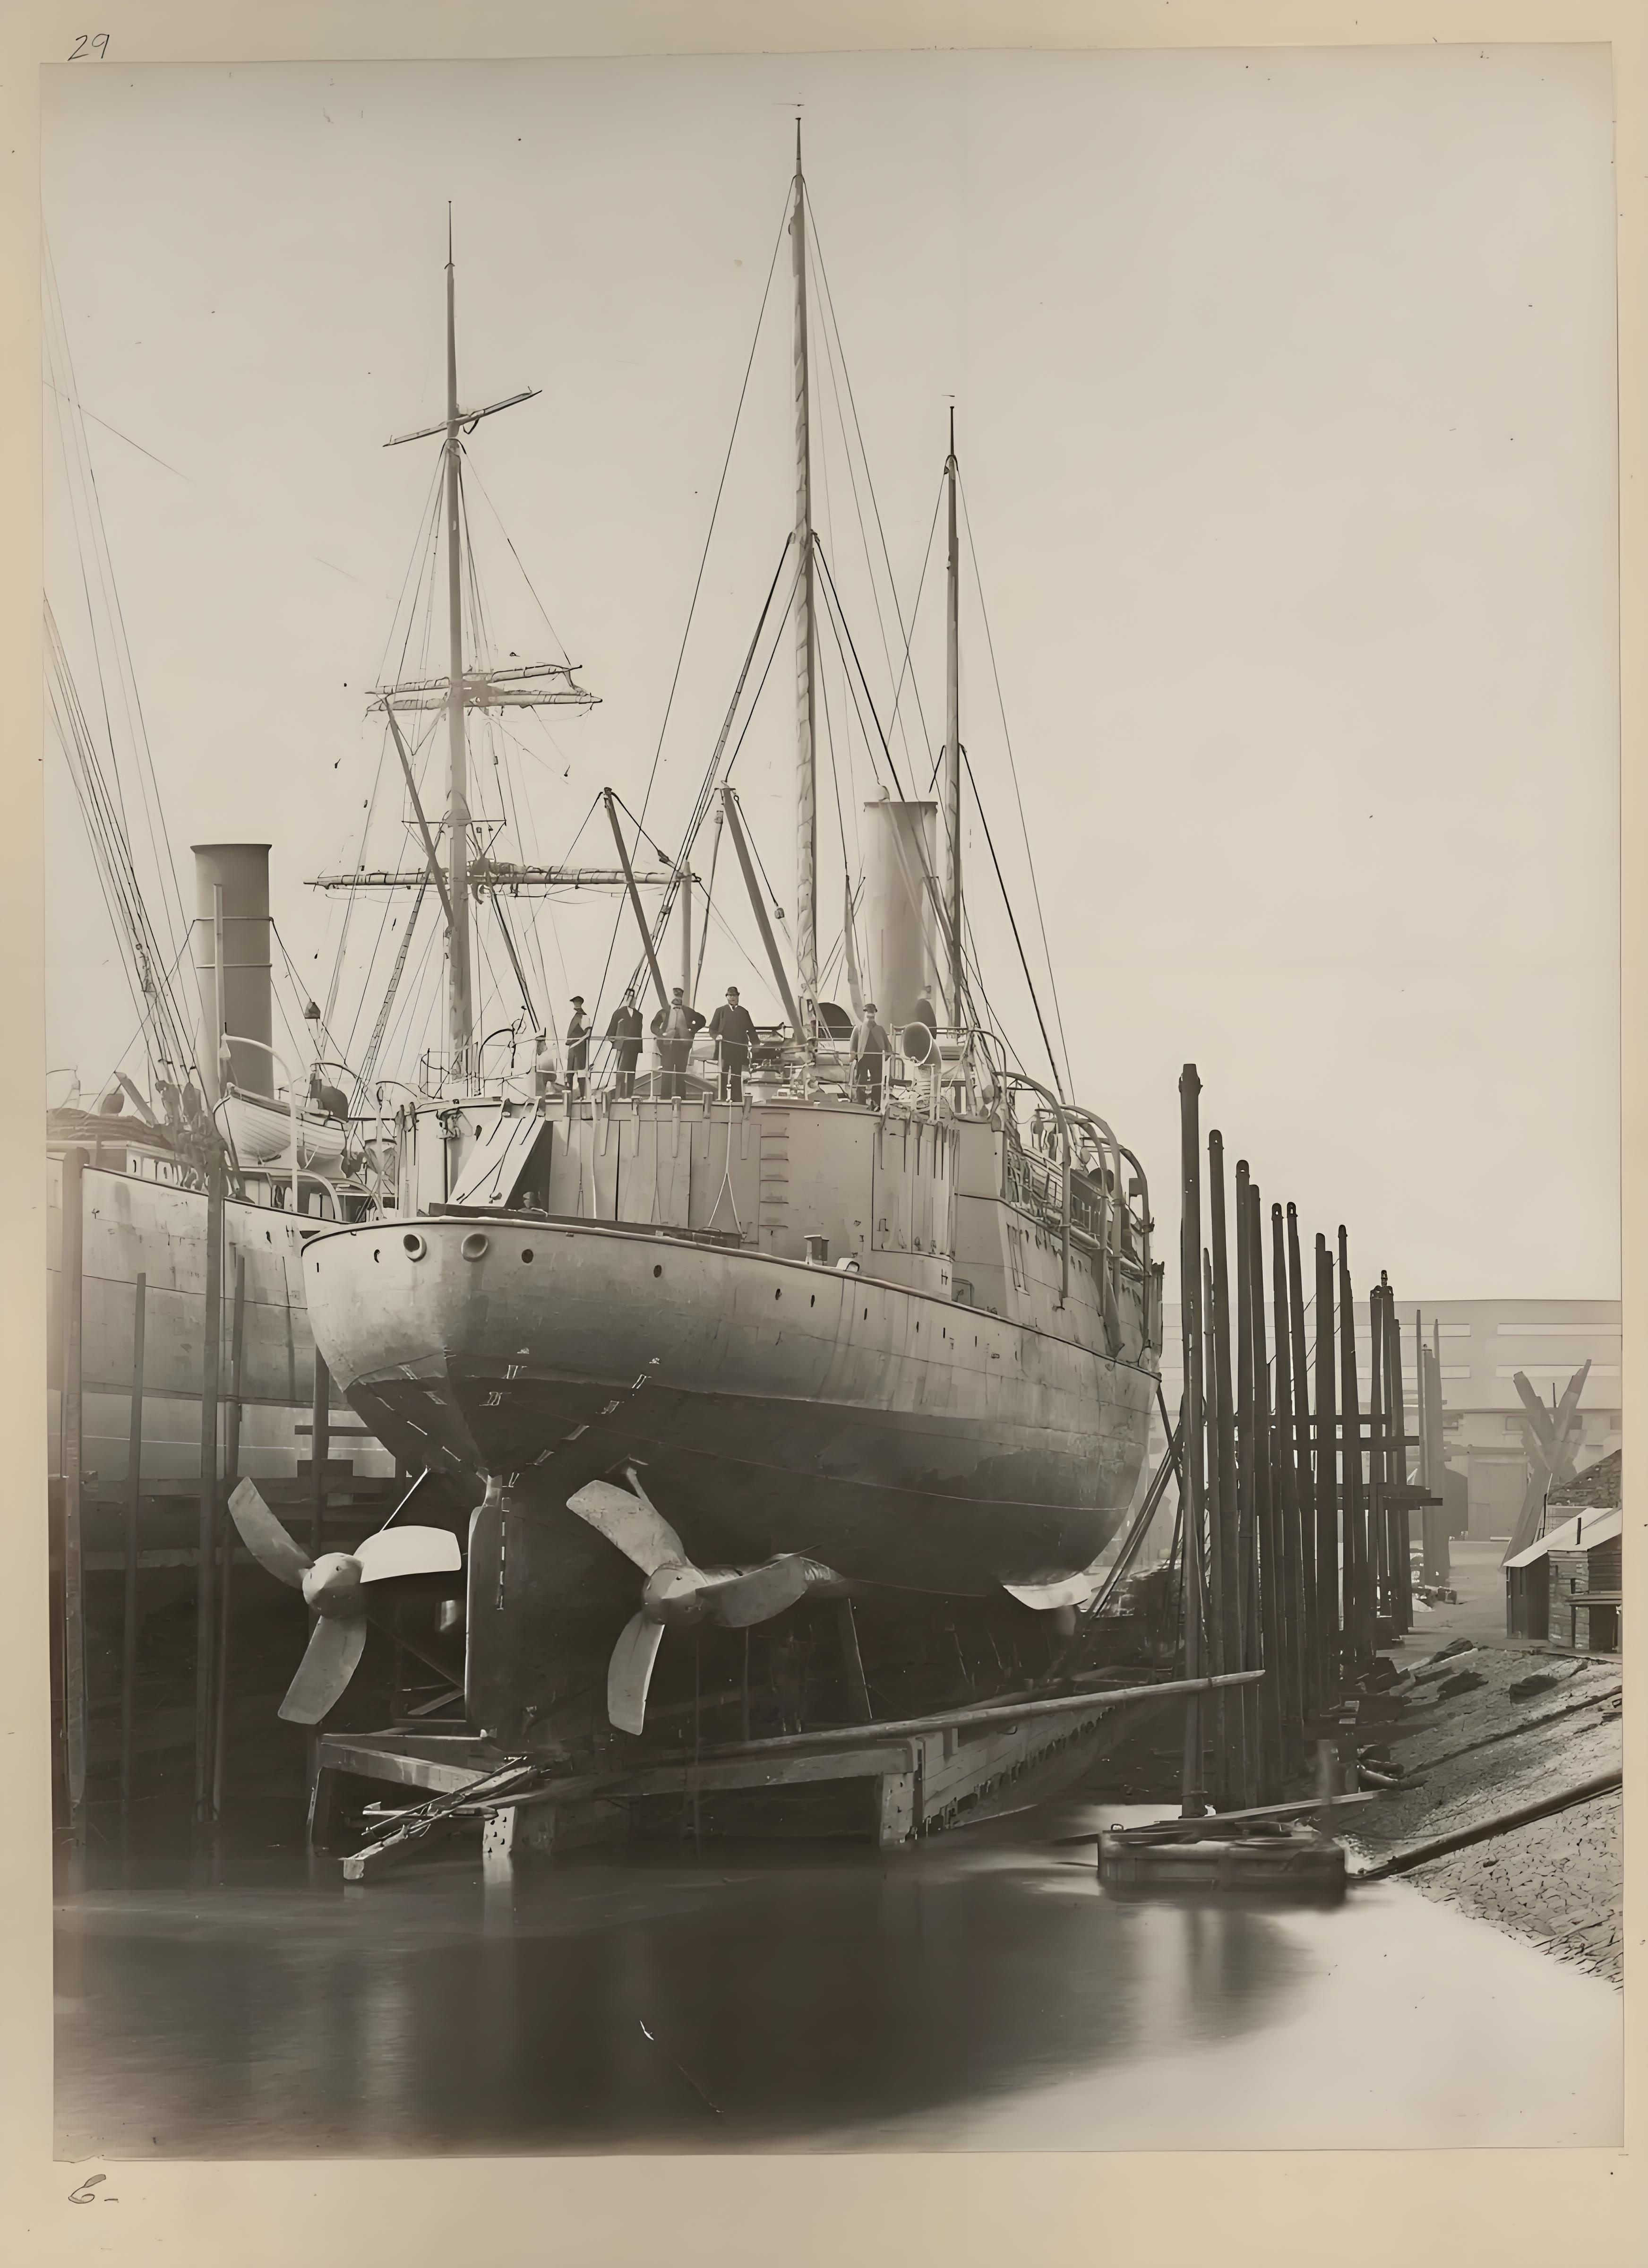
\includegraphics[width=1\linewidth]{Images/34}
	\caption{下水滑道上的“超勇”级军舰。}
	\label{fig:1}
\end{figure}

当天黄昏,一名年轻的中国海军军官登岸,夕阳下来到一座土山之上,这里安葬着接舰部队中,两位在英病逝的中国水兵:袁培福、顾世忠。墓前默哀道别之余,年轻的军官“周视良久,为之慨然”,纽卡斯尔夏季迷人的晚霞中,一位英国少女答应他将会照料这块墓地。\footnote{池仲祐:《西行日记》,北京:商务印书馆1908年版,卷下,第10页。}

\begin{figure}[htbp]
	\centering
	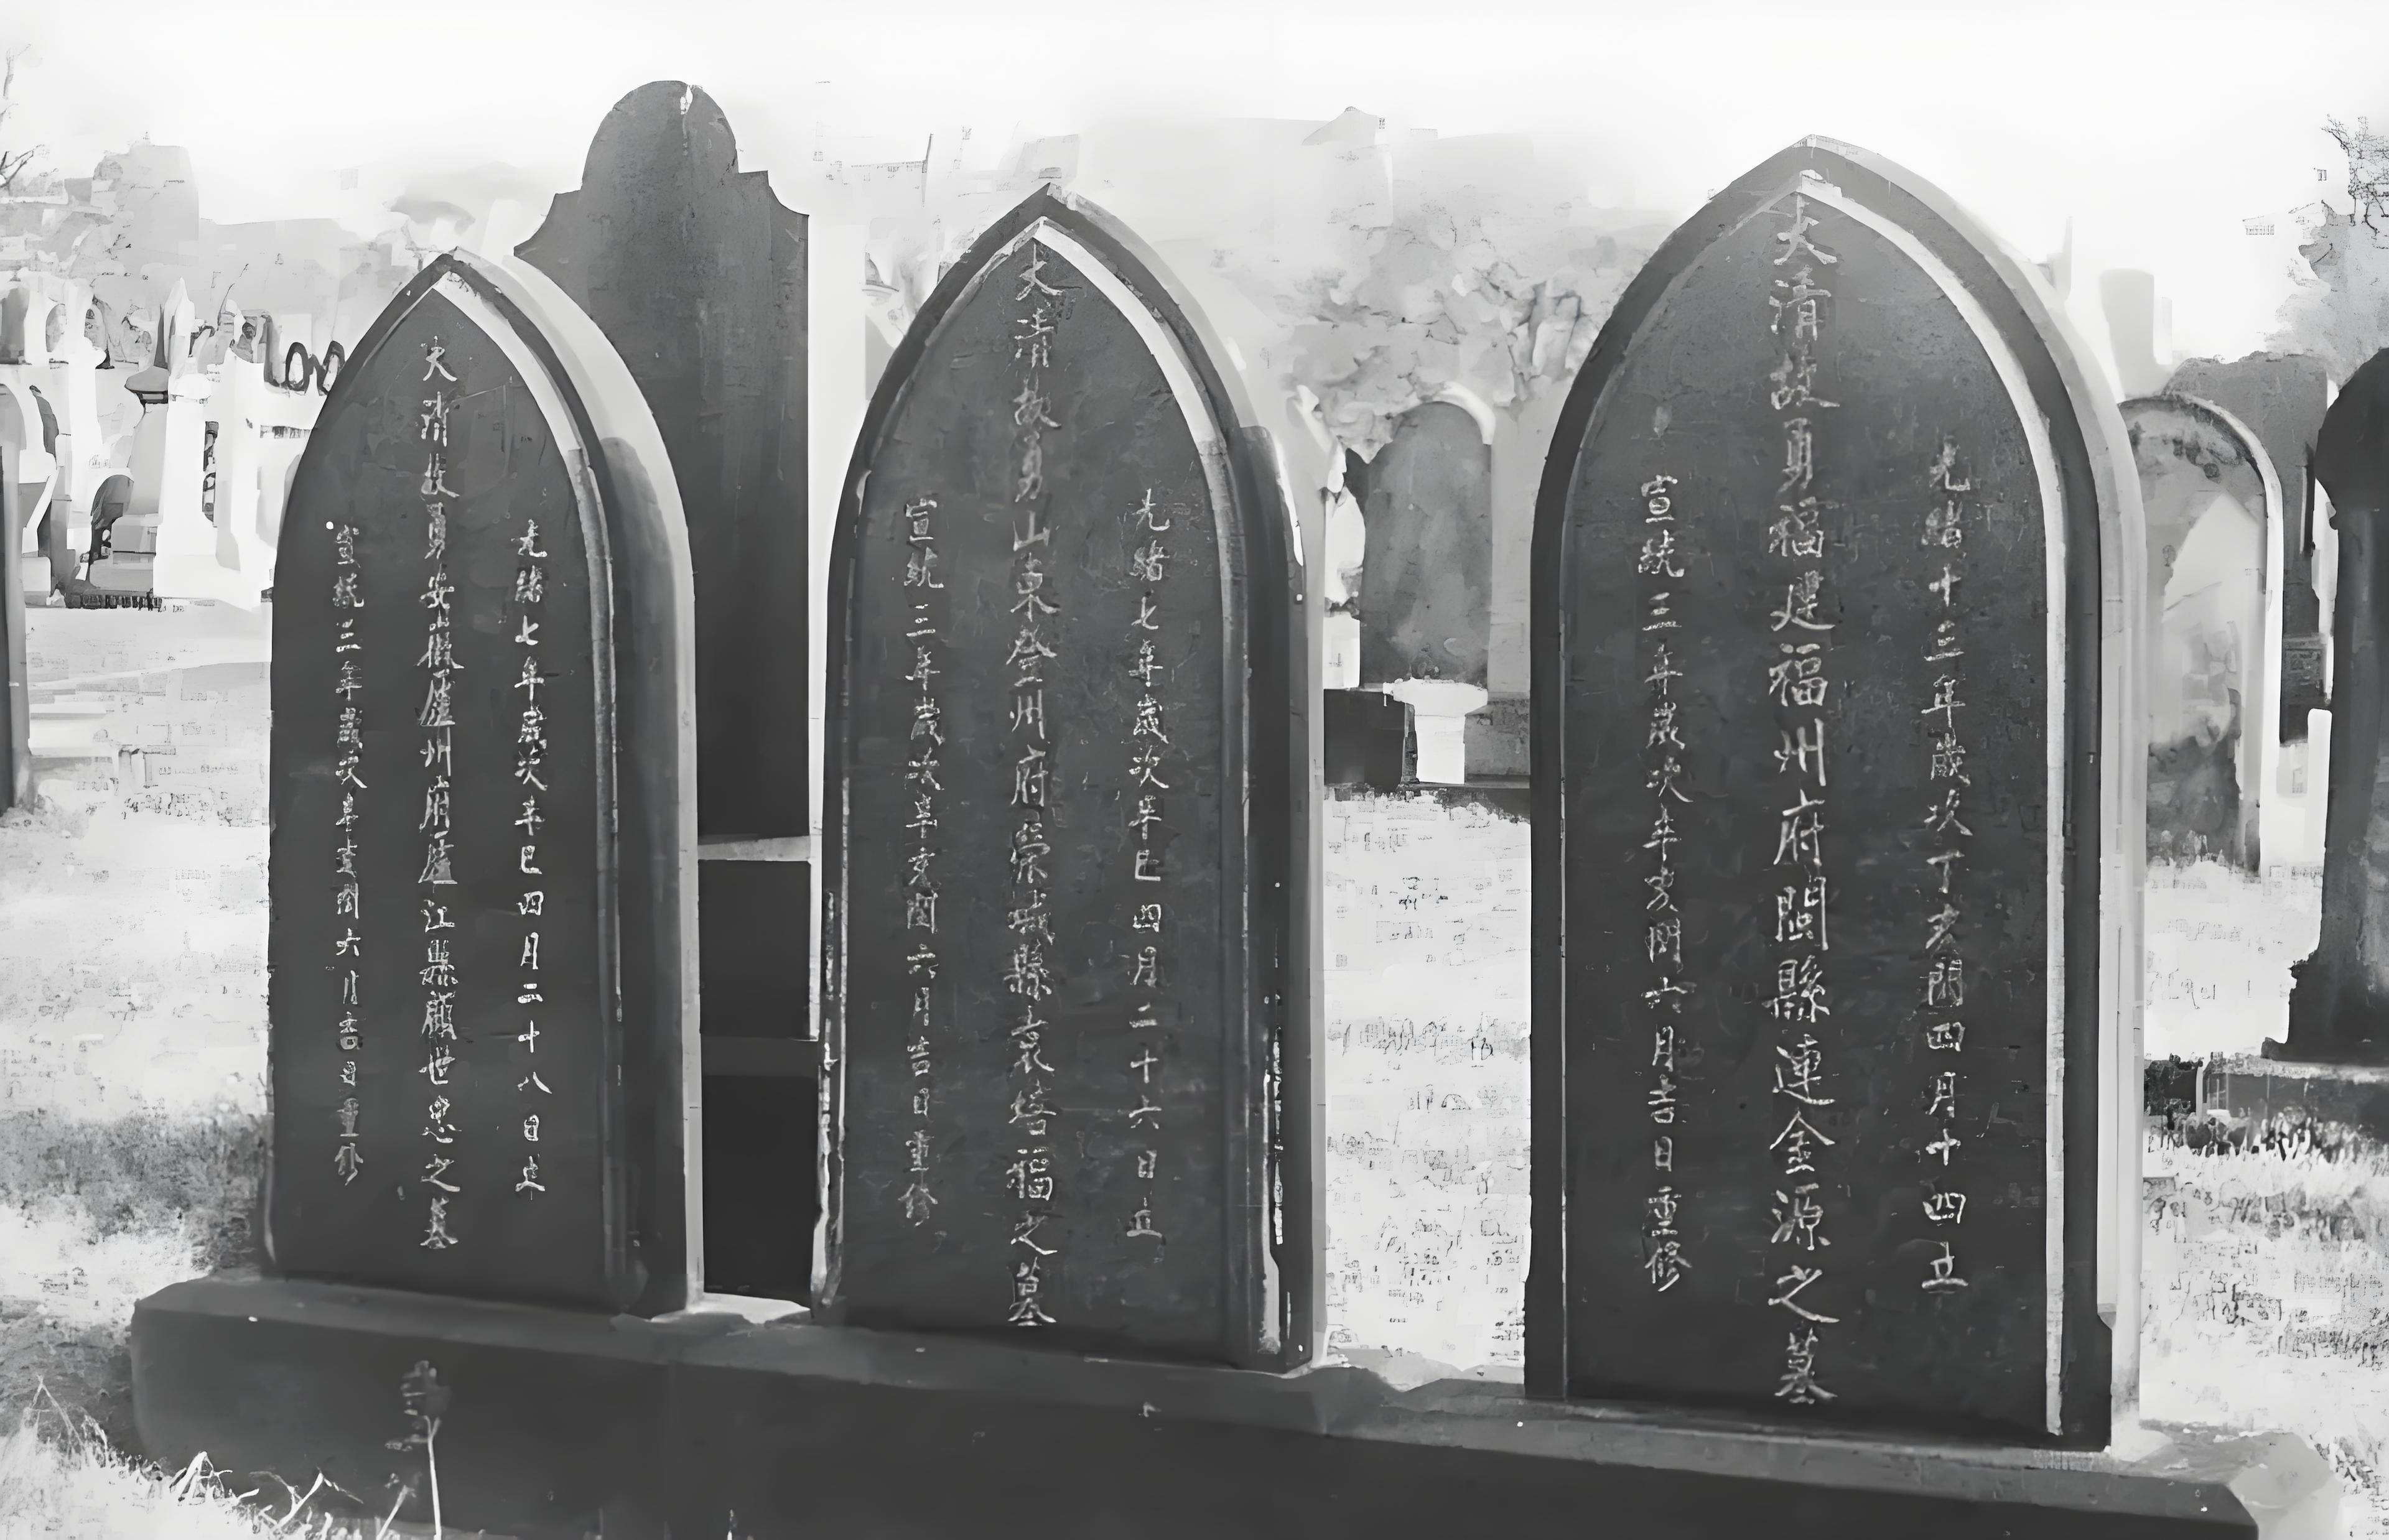
\includegraphics[width=1\linewidth]{Images/35}
	\caption{纽卡斯尔圣约翰公墓里的中国接舰水兵墓地,左侧的两块墓碑属于接收“超勇”、“扬威”时客死异国的水兵,右侧的一块则是之后接收“致远”、“靖远”时在英国逝世的水兵。3座墓碑都于1911年中国军舰“海圻”赴英参加乔治五世加冕阅舰式时重修。}
	\label{fig:1}
\end{figure}

1881年8月9日,天气晴朗。下午1点,“超勇”、“扬威”号撞击巡洋舰拉响汽笛,向她们的出生地做最后道别,“带着当地居民的最好祝愿离开纽卡斯尔”。舰上的官兵们肯定将会牢记在英国的这段日子,而纽卡斯尔市民也不会忘记这些可爱的中国水兵,“超勇”舰舷边有名年轻的军官在凭栏远眺,望着这个留下美好感情的城市越去越远,“追想旧游,不胜离思”。最初因为担心中国海军官兵的素质,而反对中国直接派人接舰的赫德显然也动了感情,称“如果船的质量是好的,中国水手们可以把船开得同英国水手们一样的安全”。

2舰于11日下午抵达英国重要军港普利茅斯,进行礼节性拜会,并与之前赴伦敦作告别拜访的丁汝昌一行会合。12日早晨,中英两国军舰在港内互相鸣炮升旗致敬,林泰曾还特意前往留学期间实习过的英国铁甲舰拜会提督、舰长等旧友。依依惜别的纽卡斯尔市此刻又发来电报,表达“中国弁兵至为良善,在英计久与本地绅民极相得,此去各有恋恋之意”。\footnote{池仲祐:《西行日记》,北京:商务印书馆1908年版,卷下,第12页。}

8月17日清晨4点,完成补给的“超勇”、“扬威”相继出港,奔向大海,踏上回国的路程。此后的日子里,这两艘高悬龙旗的军舰航行在大西洋-地中海-苏伊士运河-印度洋-太平洋航线上,途径各国均鸣炮祝贺,是为中国近代海军第一次独立远洋航行,这壮丽的远航值得永远铭记在中国海军的历史上。

但2舰的回国之路又并非一帆风顺,可谓充满惊险。先是进入地中海后不久,“扬威”与“超勇”失散,因缺煤在海上漂流了2昼夜,在距亚历山大港80海里的海面上待援,“超勇”得到消息后,前往寻获、接济方才脱险。继而,2舰过苏伊士运河时,“扬威”的螺旋桨损坏,被迫入坞修理。进印度洋后不久,“扬威”再次发生险情,先是机器出现故障,被迫停轮修理,后来锅炉舱又着火,幸好都是有惊无险。整个航程中,丁汝昌与林泰曾、邓世昌等包括外国顾问在内的全体接舰官兵尽职尽责,虽然屡次遭遇波折,但最终保证了2舰安全驶回祖国。尤值一提的是,丁汝昌在航行中,曾亲自“批阅地图”,研究制定航线,由此也可以看出丁汝昌对于海军专业知识的钻研。

经过漫长航行,1881年10月15日下午2点,狂风暴雨中,2舰驶近香港外海。水兵发现海面上有民船遇难,船民在木筏上挣扎呼救,“木排上坐六人随水漂浮而来”。当时正遇风暴,海况恶劣,干舷极低的“超勇”、“扬威”自身处境都很险恶,丁汝昌仍毅然命令“超勇”停航,援救船民,林泰曾亲自指挥收放舢板,历经惊险,将6名遇难船民“拯救到船,给食更衣,医生为之调治”,下午4时,又发现有人在岛礁上呼救,“超勇”、“扬威”再次从风浪中救起4名同胞。中国百姓第一次感受到了拥有自己海军的骄傲。

10月16日接李鸿章电报,“超勇”、“扬威”编队绕行广州、福州北上,沿海宣示主权,展现中国海军的风采。途经广州时,李鸿章的老部下,时任两广总督张树声率粤省文武官员上舰慰问犒劳海军将士。之后又经过近一个月的航行,11月18日,“超勇”、“扬威”顺利到达天津大沽,加入了创建中的北洋水师。北洋大臣李鸿章亲自到港检阅军舰、慰问将士,清政府对于接舰有功的人员也分别予以嘉奖,林泰曾被任命为“超勇”舰管带,邓世昌任“扬威”舰管带。

\begin{figure}[htbp]
	\centering
	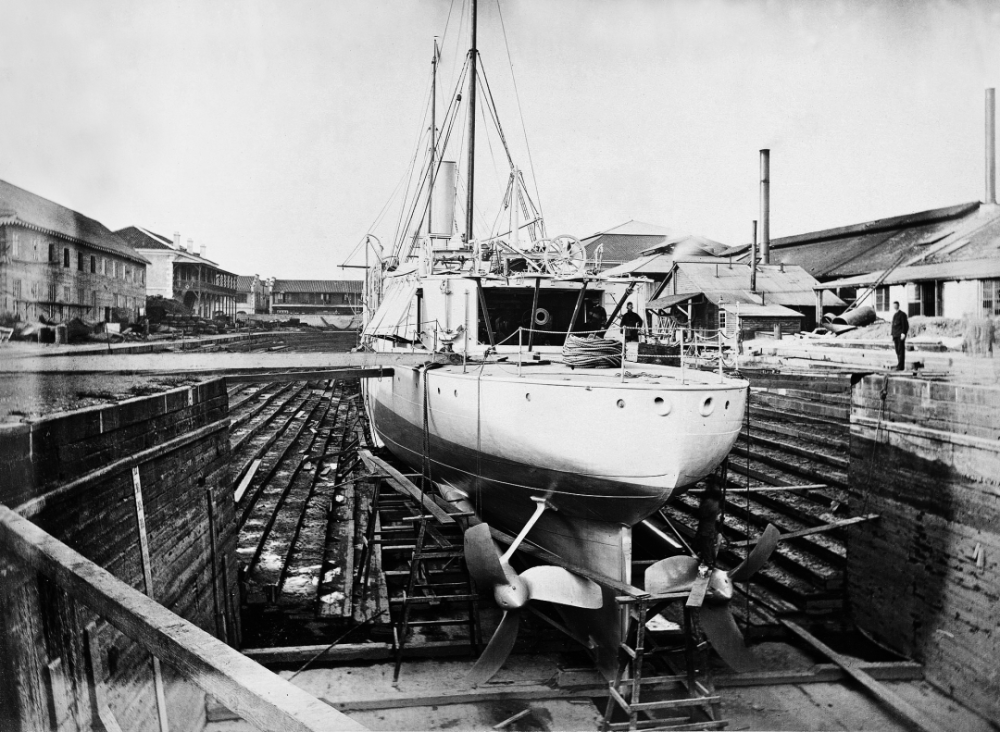
\includegraphics[width=1\linewidth]{Images/36}
	\caption{从英国抵达中国后,在上海船坞入坞维护的“超勇”级军舰。}
	\label{fig:1}
\end{figure}

“超勇”、“扬威”两艘新锐巡洋舰的加入,使得北洋海军的建军迈上一层新台阶,在2舰回国前,中国拥有的军舰除“扬武”等少数几艘旧式巡洋舰外,大都是炮船、运船和一些蚊子船,战斗力相当有限。而“超勇”、“扬威”则是当时世界著名的军舰,其武备被认为仅次于意大利的“杜里奥”(Duilio)和英国的“英弗莱息白”(Inflexible),因此在“致远”级和“经远”级巡洋舰回国之前,一直属于北洋海军的主力,在清末的几次重大政治、外交事件中均能看到2舰的身影。

\section{服役历程}

1875年,日本在朝鲜挑起“云扬号事件”,武力威逼朝鲜签订《江华岛条约》,当时限于海军力量薄弱,中国未予干涉。后为扭转日本势力侵入朝鲜的不利局面,李鸿章指示朝鲜和西方国家缔结条约,计划以此将列强力量引入半岛,从而达到制衡日本的目的。根据这一指示,1882年5月7日丁汝昌率“超勇”、“扬威”护送特使马建忠前往朝鲜,辅导朝鲜政府订立《朝美修好通商条约》。6月25日,为德国与朝鲜谈判订约,丁汝昌再次率2舰前往朝鲜。

1882年7月23日,朝鲜爆发壬午兵变,起义的士兵和平民焚毁日本公使馆、杀死日本官员,攻击闵姓贵族。控制朝鲜政局的闵妃等人逃出王宫,朝鲜陷入无政府状态。太上皇大院君李昰应借机夺取了政权。日本则趁机准备武力干涉。为抢在日军大举进入朝鲜前平息局势,“超勇”、“扬威”2舰被派往仁川,与日本军舰并泊抗衡。8月20日,由北洋水师护送,提督吴长庆部淮军4500人抵达朝鲜登陆。26日,中国军队进入汉城,丁汝昌、吴长庆以“煽动兵变”罪拘捕大院君李昰应,押送回中国囚禁。8月30日黎明,中国军队在汉城及周围地区大举镇压起义士兵,迅速平定了局势,消除了日本干涉朝鲜内政的口实。这是北洋创办新式海军以来的第一次对外行动,“超勇”、“扬威”2艘新式巡洋舰在朝鲜沿海游弋,无疑对日本海军是个极大的震慑,因为这2艘军舰的主炮可以轻而易举地撕开日本海军主力——二等铁甲舰“扶桑”的装甲。

1884年,中法因越南问题再起战事,为加强福建海防力量,“超勇”、“扬威”舰由德籍洋员式百龄(Sebelin Wallison)率领,开赴上海,准备会同南洋水师的“南琛”、“南瑞”、“开济”、“澄庆”、“驭远”组成特混舰队一起南下。在沪期间,为加强火力,“超勇”、“扬威”各加装了2门从地亚士洋行领取的37毫米哈乞开司五管机关炮。看到中国对法作战自顾不暇,日本再度在半岛挑起事端,唆使朝鲜亲日的开化党发动政变,驱逐驻朝中国军队,1884年12月4日,朝鲜开化党人发动甲申政变,趁庆祝邮政局成立之机,刺杀亲华的禁卫大将闵泳翊,勾结日军占领王宫组织新内阁。朝鲜旧臣向中国驻朝特使袁世凯“痛哭乞师”,12月6日,朝鲜军民集结数十万“将入宫尽杀倭奴”。午后,驻朝中国军队及朝鲜士兵强行入宫,宫内日军向外射击。清军在朝鲜军民支持下发动攻势,宫内的朝鲜士兵也反戈相击,日军狼狈逃窜。为稳定局势、震慑日本,丁汝昌奉命率“超勇”、“扬威”从上海北上,偕“威远”运送淮军增兵朝鲜,平息局势。由此,这两艘新锐的巡洋舰错失了一次大展手脚的机会。

1885年初,英、俄两国发生严重对抗,4月12日,英国亚洲舰队占领朝鲜巨文岛作为据点以牵制俄国。16日,丁汝昌率“超勇”、“扬威”前往巨文岛示威,与英方交涉。朝鲜政府也向英国提出抗议,英军后于1887年2月7日撤离该岛。

1886年北洋海军访问日本。

1894年5月,在大连湾参加北洋海军阅兵活动的“超勇”舰。

1887年,中国在英德两国购买的“致远”、“经远”级新式巡洋舰回国,2艘“超勇”级巡洋舰完成历史使命,从主力舰位置上退了下来,一度几乎成为练船。同年,福建船政后学堂出身的黄建勋、林履中分别接任二舰管带。

1894年,朝鲜爆发东学农民起义,应朝鲜政府请求,中国出兵平乱。“超勇”、“扬威”号和“济远”、“平远”、“威远”等北洋军舰一起担负了护送陆军前往朝鲜登陆的任务。7月25日,日军在朝鲜南阳湾外的丰岛海面偷袭中国军舰和运输船,中日甲午战争爆发。

此时的“超勇”、“扬威”服役已达十余年,昔日世界名舰的风采早已被岁月剥蚀。由于长期高强度的使用,2舰的舰体严重老化,“扬威”的锅炉更是已经到了报废的境地,昔日的飞毛腿几乎成了北洋主力舰中速度最慢者,连12节航速都达不到。但由于1890年以后,限于经费的紧张,北洋海军未能再购一舰一炮,元老舰“超勇”、“扬威”也只得老当益壮,奔赴战场。耐人寻味的是,当年在米切尔船台上的另外一艘和“超勇”级同型的智利军舰,被日本购得后,此时已经退入二线服役。

1894年9月16日凌晨,丁汝昌奉命率北洋海军主力护送陆军往大东沟登陆,“超勇”、“扬威”随队同行。17日中午11时左右,“定远”舰瞭望哨兵发现日本舰队,海军提督丁汝昌下令起锚迎战。“超勇”级军舰的起锚吊杆由于设在前后炮房的顶部,操作极为费事,然而2舰官兵凭着高涨的士气和熟练的技术,使起锚作业很快完成,“陈旧的超勇、扬威二舰,照例拔锚费时,落在后边,后亦疾驰,配置就位”\footnote{[美]马吉芬:《鸭绿江外的海战》。见日本海军军令部:《廿七八年海战史》别卷,日本春阳堂1905年版。}。

北洋舰队首先以双纵队航行,“超勇”、“扬威”作为第5小队排在队列的末尾。中午12时5分过后,北洋舰队变换为夹缝雁行阵,迎击日本联合舰队,类似利萨海战中奥地利舰队用来打败意大利舰队的横阵,以当时北洋海军主力各舰的射击特点而言,这无疑是最实用的阵形。在纽卡斯尔诞生的同胞姊妹“超勇”、“扬威”被配置于阵形的右翼翼端,丁汝昌这一安排,可能是考虑以此保护这两艘无防护的老式巡洋舰,因为成纵队而来的日本舰队,如果要攻击处于右翼的“超、扬”,势必要从北洋舰队阵前航过,将侧面完全暴露在中国军舰舰艏方向的火力下,按正常思考是不会冒这个风险的。

但是,出乎所有人的意料,日本舰队因为发生严重的指挥失误,在北洋海军阵前突然向左大转弯,矛头直指位于右翼末端的“超勇”、“扬威”2艘弱舰。事后,美国海军军官马汉(Alfred Thayer Mahan)在评论这段历史时,毫不客气地指出“日军通过清军前面后,向右翼突进。采取这种前面通过的运动法理由何在?我实在难以理解。这恐怕是为了把炮火集中敌之右翼这一最终目的,而甘冒非常之险”,认为日本舰队的此种做法“使自己舰队的侧面,暴露于舰艏向我的敌阵,实乃无谋之策”\footnote{《评鸭绿江口外的海战》,中国近代史资料丛刊续编《中日战争》7,北京:中华书局1996年版,第320--321页。}。

为充分发扬横阵的特点,以及北洋海军各舰舰艏方向火力较强的优势,12时48分,在6000米距离上,中国旗舰“定远”右侧主炮台的305毫米口径巨炮发出一声怒吼,向正在通过北洋海军阵前的日舰发起攻击,闻名中外的黄海海战就此打响。随后,中国舰队各舰陆续发炮,虽然接连有日本军舰中弹,但中国各舰火炮射速过慢,无法在短时间内给日方造成重大损伤。

由“吉野”、“高千穗”、“秋津洲”、“浪速”组成的日方第一游击队,利用其舰龄短、航速高的特点,高速运行到中国舰队右翼。12时55分,距离3000米时,“吉野”上的速射炮猛烈开火,随后3舰也陆续开始射击,弹雨向“超勇”、“扬威”倾泻而来。

面对如狼似虎的日本第一游击队,处于绝对劣势的“超勇”、“扬威”舰仍拼死作战,2舰官兵在恶劣环境里,不屈不挠地进行还击,体现了中国海军军人的骨气。13时8分,“超勇”、“扬威”击中“吉野”舰的后甲板,引爆了露天堆放的弹药,“吉野”顿时冒起浓烟。几乎同时,“高千穗”、“秋津洲”也先后被击中受伤,紧接着“浪速”也被命中。然而10余年前的世界名舰“超勇”、“扬威”终究敌不过1894年的世界名舰,这是一个弱肉强食的时代,海军技术的发展一日千里,停滞不前只有被动挨打。

2-10

黄海海战中,日本摄影师在西京丸上拍摄到的“超勇”舰遗影。照片中位于左、右两侧的分别是“千代田”、“严岛”,中央远处发散浓烟的地方,就是正在起火燃烧的“超勇”。

13时20分,一颗敌弹射入早已创伤累累的“超勇”舰舱内,引发大火,全舰顿时被浓烟笼罩。灾难就此降临,四散的火焰根本无法控制,“超勇”舰成了一团火球。日方的攻击越来越猛烈,“超勇”逐渐向右倾斜,但“犹以前部炮火发射不停”,最终于14时23分沉没于黄海的怒涛中。管带黄建勋落水后拒绝救援,随舰同沉。

“超勇”燃起大火的同时,姊妹舰“扬威”也在日方打击下遭到重创,同样燃起了灾难性的大火。管带林履中、三副曾宗巩等一面组织救火,一面继续发炮抗敌,但在日本第一游击队的轮番轰击下,伤势过重,液压系统遭到破坏,“首尾各炮,已不能动”,而“敌炮纷至”。浓烟滚滚的“扬威”最终选择驶离战场施救,拼命向大鹿岛附近的浅水区驶去,因为日本军舰吃水普遍较深,浅水区就成了中国海军天然的避风港。在这决定生死的航程上,一幕最无法想象的事情发生了,高速逃跑中的“济远”号巡洋舰撞上了早已遍体鳞伤的“扬威”。大量进水的“扬威”虽然仍在苦苦挣扎,努力向浅水区航行,但终于愈行愈滞,渐不能支,舰身渐渐沉于大海。管带林履中悲愤万分,毅然蹈海自尽。黄海海战后的次日,日本联合舰队重返海战场检查,发现“扬威”舰还有部分残躯没有完全沉没,于是由“千代田”号装甲巡洋舰近距离发射鱼雷,“扬威”彻底从海面上消失了。

“超勇”、“扬威”就这样消逝在了血与火的战场上,结束了虽然短促,但无比壮丽的一生,和与她们同命运共生死的官兵一起静静的躺卧在黄海海底。不知道在2舰生命的最后一刻,是否有水兵想起那万里之遥的纽卡斯尔?

那位曾经久久伫立在纽卡斯尔港畔的年轻人,于1926年编撰了记载清末海军历史的《海军实记-述战篇》,为他服役过的军舰和曾朝夕相处的战友们作传。“……‘超勇’、‘扬威’两舰中弹火发,全舰焚毁。‘超勇’管带黄建勋、‘扬威’管带林履中,浮沉海中,或抛长绳援之,推不就以死,各员兵弁均随船焚溺……”\footnote{池仲祐:《海军实记》述战篇,“甲午战事纪”。}不知道池仲祐写下这段泣血的文字时,是否还会想起那场1881年夏天纽卡斯尔的梦。

2002年,山东省威海市档案局档案查取小组远赴英伦,调查、征集中国近代受甲午战争影响而开始的“英租威海卫”历史档案。寻找资料之余,调查小组意外在纽卡斯尔发现了一处百年前的中国海军墓地,墓碑上铭刻着长眠在此的两位中国威海籍水兵的名字:“大清故勇袁培福、顾世忠”。

\begin{quotation}
大地再没有比这儿更美的风貌:

若有谁,对如此壮丽动人的景物,

竟无动于衷,那才是灵魂麻木;

瞧这座城市,像披上一领新袍,

披上了明艳的晨光;环顾周遭:

船舶,尖塔,剧院,教堂,华屋,

都寂然、坦然,向郊野、向天穹赤露,

在烟尘未染的大气里粲然闪耀……

\begin{shuming}
—— [英] William Wordsworth(华兹华斯)
\end{shuming}

\end{quotation}

\chapter{失落的辉煌(上)——中国铁甲舰前史}

1874年春天,清王朝福建省管辖下的台湾岛被一场突如其来的风波侵袭,成了整个帝国关注的焦点。5月22日,日本明治政府“台湾番地事务都督”西乡从道率军在台湾南部的社寮海岸(今为台湾屏东县境内)登陆,以“征番”为借口,大肆攻打、焚掠台湾番社,并有久占之势。

面对突发的日本侵台事件,清王朝满朝震惊不已,立即设法针锋相对,派遣驻节福州马尾的总理船政大臣沈葆桢率军舰、兵勇渡海调查、抗衡。

沈葆桢,字翰宇,号幼丹,1820年4月9日出生于福建侯官(今属福州市),是清末名臣林则徐的外甥、女婿,进士出身,曾任江西巡抚,又作为首任船政大臣成功主持了船政的中外技术合作事业,颇著政声。船政事关工业、教育、海军以及中外交涉等诸多事务,沈葆桢亲力亲为,也因此沈氏是当时整个帝国官场上最具近代化海防实务经验的高级官员。

首任总理船政大臣沈葆桢

5月29日,鉴于日本侵台的形势吃紧,清王朝又颁旨授予沈葆桢“钦差办理台湾等处海防兼理各国事务大臣”头衔,授权沈葆桢与日方直接交涉折冲,并给予其调度福建省官员、军队以及江苏、广东等省近代化舰船的军政权限,以便临机应变。

几天过后,沈葆桢于6月3日将自己所思考的处置方略上陈清廷,以“联外交”“储利器”“储人才”“通消息”作为应对、平息日本侵台挑衅的四大端绪。在其中的“储利器”一节中,沈葆桢提起了一种名为铁甲船的海上利器。从此,一场地方大员为了获取制海利器的努力史也就此揭幕。

\section{“铁甲船不容不购也”}

沈葆桢在1874年6月3日上奏中提到的铁甲船,就是英文所称的Ironclad,今译铁甲舰、装甲舰,是那个时代海洋上的霸主。

如果把海军的舰船体系视作一个大海上的特殊生物圈系统,随着科技的演变,占据在这个生物圈顶层的军舰种族也在应时而动,不断发生着变化。18、19世纪,是木质风帆战列舰(ship of the line)称王称霸的时代,世界海军中最具威力的主战军舰是具备有多层炮甲板的大型木质风帆战舰,这种船身高大,舷侧密布着一层层黑洞洞炮门的大帆船,炮火凶猛,是那个时代海洋国家的实力象征。

进入19世纪后,蒸汽机的出现革命性地改变了海军舰船的发展方向,蒸汽驱动的机械动力逐渐取代风帆,解决了动力自由的舰船开始有了更多的设计可能性。1860年,法国建成了人类历史上第一艘大型蒸汽动力铁甲舰“光荣”号(Gloire),在木制的舰体上,军舰舷侧附着安装了厚度120毫米左右的铁板装甲,使得军舰可以抵御炮弹的袭击,防护力大大提升。紧随其后,英国在1861年建成了规模更大的“勇士”号(Warrior)铁甲舰。这两艘军舰的出现,标志着铁甲舰时代的到来。

军舰披挂上装甲,兼具攻击力和更强的战场生存力,其军事价值显而易见,从19世纪60年代开始,西方海洋国家开始纷纷建造、装备铁甲舰,铁甲舰的设计也在不断演变进化,既包括有排水量在万吨左右的大型铁甲舰,也不乏仅仅只有数千吨甚至更小的小型铁甲舰,这些军舰都是海军中冲锋陷阵的主战军舰,其中的大型铁甲舰更是成了衡量一个海洋国家国力强弱的新标志。

世界第一艘大型蒸汽动力铁甲舰“光荣”号

世界海军迈入铁甲舰时代的时候,清王朝统治下的中国刚刚经历第二次鸦片战争和太平天国农民起义的沉重打击,为求自强,中央与地方一些开明大员开始努力推动近代化事业,尤其聚焦于军事自强、海防自强。后者的主要目标,在于使中国的海上力量尽快实现蒸汽动力化,以抗衡西方列强的坚船利炮。

1866年,闽浙总督左宗棠上奏获准,在福州马尾设立总理船政,聘请法国人日意格(Prosper Marie Giquel)为洋员正监督,雇募西方技术团队帮助实施舰船和海军科技的对华输入,旋后沈葆桢出任首任总理船政大臣,船政成为当时全国近代舰船的研发建造中心。几乎同时,位于上海的江南机器制造总局也开展舰船建造事业,形成了与船政遥相呼应的态势。由于当时中国没有任何近代化舰船的技术基础,迫切想要解决的首要问题是“能造”,为了尽快迈入蒸汽动力舰船的技术大门,船政与江南早期的舰船建造都选择了相对技术难度小、资金投入较少的炮舰、运输舰等舰型,而并没有企及作为主战军舰的铁甲舰。

在沈葆桢奉命钦差赴台湾抗衡的1874年,中国海防线上的蒸汽动力军舰大多是排水量2000吨级以下的炮舰、炮艇,总体上与西方同类军舰的性能接近,数量规模上甚至超过了日本。但是,日本海军的阵营中此时早已有了主战军舰——铁甲舰,而且有2艘之多。

日本近代海军的起步时间与中国相近,不过由于幕末长年内战,受战场需要的直接刺激,幕府政权与一些地方强藩都努力装备更强的舰船,其获取舰船装备的动作幅度要比清王朝大得多。

1869年,日本幕府政权从美国购买了1艘法国设计建造的小型铁甲舰“石墙”(Stonwall),抵达日本后最初称为“甲铁”,后来更名“东”,明治政府成立后收编入国家海军。这艘军舰的排水量虽然只有区区1358吨,其装备的1门11英寸口径的前膛主炮却可以击穿1874年时所有的中国军舰,而“东”舰的舰体装备了厚度为90至125毫米厚的熟铁装甲,主炮炮房更是敷设了厚度为102至140毫米厚的装甲,这些防护在当时几乎可以抵御任何一艘中国军舰的炮火攻击。\footnote{《日本军舰史》,青岛:青岛出版社2016年版,第5页。}

日本小型铁甲舰“东”

日本海军的另外一艘铁甲舰名为“龙骧”,原本是熊本藩在英国订造的小型铁甲舰,建成后于1870年上缴明治政府。这艘军舰的排水量2571吨,火炮数量多,火力凶猛,安装了2门口径160毫米、10门口径140毫米的克虏伯炮,军舰的舰体安装厚度125毫米的装甲,同样是当时中国军舰的舰炮所无法击穿。\footnote{《日本军舰史》,青岛:青岛出版社2016年版,第6页。}

1874年奉命钦差赴台平息事变时,沈葆桢已清晰地掌握了日本装备2艘铁甲舰的情况,而且对铁甲舰的军事价值有了充分的认识。在向清政府奏报方略的奏折里,沈葆桢表达了对这一情况的深深担忧,“该国尚有铁甲船二号,虽非完璧,而以摧寻常轮船则绰绰有余。彼有而我无之,水师气为之夺”,认为解决办法惟有尽快装备铁甲舰,“两号铁甲船不容不购也”。\footnote{《文煜等奏遵旨会办台湾防务情形并敬陈管见折》,《筹办夷务始末·同治朝》10,北京:中华书局2008年版,第3760页。}

主持船政、亲身经历过近代化舰船缔造事业的沈葆桢,对海军装备的重要性格外敏感。日本其志不小,为了惩前毖后,中国在装备上不能落人后,从此以后,沈葆桢的海防、海军建设思维版图中,购买铁甲舰一事占据了重要的位置。

\section{布国铁甲船}

对船政事务作出一番布置后,沈葆桢率日意格等随员于1874年6月14日分乘船政轮船舰队的千吨级炮舰“安澜”“飞云”从福州马尾出发,出闽江进入大海,巡视厦门、澎湖等海防要地,而后径驶台湾。

沈葆桢乘舰出发的当天,千里之外的北京城中,清政府就6月3日沈氏的上奏作出了上谕指示,针对沈葆桢提到的铁甲舰问题,清政府批准“照所议行”,允许沈葆桢着手购买铁甲舰,购办铁甲舰的相关经费由福建省筹措“将闽省存款,移缓就急,酌量动用”,并批准倘若福建省的经费不足支付,允许沈葆桢在国际市场拆借资金,“如有不敷,即照所请暂借洋款,以应急需”。\footnote{《廷寄》,《筹办夷务始末·同治朝》10,北京:中华书局2008年版,第3760页。}

6月17日,沈葆桢抵达台湾安平港,登上台湾岛。海峡航行的实际感受,以及在台湾岛的所见所闻,更加深了沈葆桢要快速购办铁甲舰的信念,“铁甲船亦不可无,无则过台弁兵、军装必为所截掠。倭奴以孤军驻琅峤而无所惧者,恃有此耳。”\footnote{《沈葆桢致李鸿章》,《从船政到南北洋——沈葆桢李鸿章通信与近代海防》,福州:福建人民出版社2020年版,第66页。}随着清政府上谕到达台湾,沈葆桢购办铁甲舰的努力就此正式着手实施,显露出沈氏一贯的风风火火作风,其最初映入世人眼帘的,是一艘“布国铁甲舰”。

具体办理寻购铁甲舰事宜的原船政洋员正监督日意格。

“布国”即普鲁士(Prussia)。得到清王朝授权后,沈葆桢将寻购铁甲舰的工作具体委托给原船政洋员正监督、法国人日意格。在当时,要快速获取铁甲舰,最直接的办法就是转买别的国家现成的铁甲舰,日意格以上海为信息中心,开始四处打听,在1874的7月前后捕捉到了一条信息,即普鲁士海军的一艘铁甲舰有意变卖出售。

日意格当时发现的布国铁甲船,极有可能是普鲁士海军的“阿德尔伯特亲王”(Prinz Adalbert)。这艘军舰是普鲁士/德国海军装备的第一艘铁甲舰,非常巧合的是,“阿德尔伯特亲王”号与当时日本海军装备的“东”号铁甲舰还是源出同门的同型姊妹舰。

该舰和日本的“东”号都是美国南方邦联在法国波尔多订造的军舰,原本计划投入南北战争,该舰原定舰名“基奥普斯”(Cheops),1865年建成时美国南北战争已经结束,被转卖给了普鲁士,更名“阿德尔伯特亲王”。该舰排水量1535吨,武器配置与姊妹舰“东”略有区别,主炮是1门210毫米口径炮,配合2门170毫米口径副炮,舰体装甲厚127毫米。编入普鲁士海军后,该舰的木制舰材出现腐朽等问题,舰况长期不佳,在1871年除役,成为闲置的封存舰。\footnote{Conway's All The World's Fighting Ships 1860--1905,Conway Maritime Press1979,p242.}未能料到的是,几年之后竟然吸引了来自中国的目光。

经对这艘现成可售的布国铁甲船稍加了解,日意格、沈葆桢都发现了这艘军舰舰况太差的问题,立刻打消了转购的念头,调整目光,寻找新的目标,“日耳曼铁甲船水缸太旧,不可用”。\footnote{《沈葆桢致李鸿章》,《从船政到南北洋——沈葆桢李鸿章通信与近代海防》,福州:福建人民出版社2020年版,第73页。}

\section{英国铁甲船}

替代普鲁士铁甲舰的,是一组英国铁甲舰。日意格从洋行处了解到,有7艘英国铁甲舰可以转售,基于经费等考虑,沈葆桢对其中体量最小的表示青睐,“闻英国七号内有一小而完者,当议购也”。对照当时英国皇家海军的舰船序列,所指的极有可能是英国的“企业”号(Enterprise)小型铁甲舰。

英国铁甲舰“企业”(右)

“企业”号排水量1350吨,建成于1864年,军舰舷侧装有114毫米厚的铁质装甲,舰上的武器最初为100磅和110磅炮各2门,1868年更换为4门177毫米口径火炮。\footnote{Conway's All The World's Fighting Ships 1860--1905,Conway Maritime Press1979,p12.}这艘军舰在1871年转入后备役,日意格四处打听二手铁甲舰转卖信息时可能得到了该舰的信息。

超出日意格乃至沈葆桢意料的是,物色铁甲舰出售信息一事,引起了英国在华利益代言人的注意。

1874年8月16日,李鸿章致信告诉沈葆桢,海关总税务司赫德在总理衙门参了日意格一本,开始插足铁甲舰事务。日意格早年曾在海关任职,担任过宁波税务司,因为直接与左宗棠合作创办船政,引起赫德的不快,二人存在嫌隙。李鸿章向沈葆桢透露,赫德在总理衙门声称听闻“中国某省托外国洋商购铁甲船,此洋商曾在中国开行两次闭歇者”,言下之意是寻购铁甲舰所托非人,直接影射日意格,同时赫德还提出了小铁甲舰无用的观点,认为如果要购买铁甲舰,应该直接购入大型舰,“铁甲船总须一、二等佳者,若购三、四等仍无用,不如贵价买好货”。赫德就此向总理衙门提出建议,直接通过英国驻华公使威妥玛(Thomas Francis Wade),从政府层面寻购英国的二手铁甲舰。\footnote{《李鸿章致沈葆桢》,《从船政到南北洋——沈葆桢李鸿章通信与近代海防》,福州:福建人民出版社2020年版,第75--76页。}

总理衙门认为赫德所述的模式显然更稳妥可靠,李鸿章也同意这一判断,在信中建议沈葆桢命令日意格与威妥玛“酌办”,言下之意乃是应让日意格退出寻购铁甲舰的活动。对于日意格,李鸿章早就认为其在参与船政等工作时开价过巨,手笔过辣,并不具有好感。

面对李鸿章以及总理衙门的意见,沈葆桢内心疑惑犹豫。沈葆桢随后致信将这起节外生枝的风波通报日意格,信中并未要求日意格将购买铁甲一事与英国公使威妥玛协商,但沈葆桢似乎受到了“所托非人”问题的影响,向日意格强调“如英国有佳者可购,则购之,倘无可购,不如请阁下回闽厂添买机器自造”,即倘若寻购铁甲舰并无可靠把握,不如改换路径,设法在船政自造。

\section{丹国铁甲船}

1874年9月2日,沈葆桢回信李鸿章,没有就李来信所通报的铁甲舰问题进行正面答复,也不再提起日意格之前寻购的布国铁甲船和英国铁甲船,而是告诉李鸿章,日意格已经谈成了一艘“丹国铁甲船”,而且显得事已定局的是,日意格甚至连这艘军舰未来的舰长人选都已物色好,即由船政后学堂第一届外堂毕业生张成担任。\footnote{《沈葆桢致李鸿章》,《从船政到南北洋——沈葆桢李鸿章通信与近代海防》,福州:福建人民出版社2020年版,第84页。}

“丹国”即欧洲国家丹麦,“丹国铁甲船”则是指丹麦海军的“丹麦”号(Danmark)铁甲舰。这艘军舰排水量4670吨,属于中型铁甲舰,舰上装备了超过20门舰炮,舰体侧面敷设厚度为114毫米的铁质装甲。\footnote{Conway's All The World's Fighting Ships 1860--1905,Conway Maritime Press1979,p364.}相比起此前物色的布国铁甲船和英国铁甲船,“丹麦”号的总体设计较为陈旧,属于将火炮沿船舷布置的船旁列炮铁甲舰,但是其体型大,对当时的东亚国家来说无疑是艘巨舰,对抗日本的“东”和“龙骧”具有很大的优势。

“丹麦”号和日意格此前打听到的“布国铁甲船”身世十分相似,也是美国南北战争期间南方邦联在欧洲订造的军舰。1862年,美国南方邦联代表在英国订造了该舰,起初想要以该舰占取相对于北方联邦的绝对海上优势,而后随着战局变化,在1863年决定将建造中的该舰变卖,等到该舰在1864年建成时,丹麦和普鲁士之间爆发第二次石勒苏益格战争(Danish-Prussian War),丹麦为了尽快加强海上力量,从英国转购了这艘崭新的中型铁甲舰,命名为“丹麦”,由于舾装等工作延期,该舰未来得及加入战争。1865年丹麦和普鲁士的战争结束后,这艘体型较大的铁甲舰对丹麦海军失去意义,被转入预备役,具有了转售的可能。

丹国铁甲船“丹麦”

1874年,日意格在上海通过旗昌洋行居间打听到这艘闲置的欧洲铁甲舰,经过商洽接触,谈判深入到了讨论价格的实际操作环节,最后议定转卖价为100万两银,卖方要求首先支付一半费用作为定金,另一半则等到该军舰从丹麦驶抵中国交付后付清。根据清廷此前作出的由福建省承担铁甲舰购买费用的谕示,被沈葆桢请在马尾坐镇船政的船政稽查林寿图开始办理具体的请款事宜,向闽浙总督李鹤年协商。未料,李鹤年受总理衙门想要通过英国公使馆购舰思路的影响,且自身对日意格存在不信任,并不放心直接从福建藩库直接拨付定金,而是希望由日意格自行借贷、筹款,先支付定金,等正式请旨批准此事后再拨款归还给日意格。

沈葆桢得知这一情况,颇为气恼,认为是闽浙总督有意推诿,于是指示林寿图尽力与之辩争。由于对闽浙总督并无节制管辖之权,倘若其在付款问题上继续推脱,沈葆桢表示也无可奈何,只能作罢。为了负责起见,沈葆桢同时向林寿图表示,如果日意格已经和丹麦方面订立了合同,最终因为无法付款而导致合同作废,丹麦方面追索违约赔偿时,将由船政承担这些费用。\footnote{《沈葆桢致林寿图》,《从船政到南北洋——沈葆桢李鸿章通信与近代海防》,福州:福建人民出版社2020年版,第86--87页。}

正当各方聚焦于如何筹措购置铁甲舰的经费时,作为居间人的旗昌洋行传来令人意外的消息,丹麦方面突然反悔,不愿向中国出售“丹麦”号,此事无疾而终。

\section{从长计议}

从“布国铁甲船”“英国铁甲船”,再到“丹国铁甲船”,沈葆桢通过日意格寻购铁甲舰的努力接连遇到坎坷。在当时,沈葆桢之所以急于购成铁甲舰,最重要的原因是日本侵台事件带来的军事压力迫在眉睫,一旦中日外交决裂,两国军舰海上交锋的后果不堪设想,沈葆桢渴望迅速将中日两国间的海上实力扳平,为此将获取铁甲舰的着眼点放置于购买外国现成的军舰,重中之重在于军舰是否为现货,至于舰龄、设计等等都暂在其次。客观而言,购舰急就章未能立刻谱成,实际上使中国获取铁甲舰的努力更为稳健。

巧合的是,就在求购“丹国铁甲船”的计划落空时,以外交途径解决日本侵台事件的工作收获重大成果。在英国的斡旋下,中日两国代表经过在北京的反复谈判,于1874年10月31日达成协议,签订《北京专条》,清政府付出赔偿军费等代价,日本则将军队撤离台湾,日本侵台事件得以化解。

台湾海峡上空的乌云渐散,铁甲舰已非燃眉之急,沈葆桢获得了深入思考铁甲舰问题的时间。也就在这时,受日本侵台事件的刺激,感到“若再不切实筹备,后患不堪设想”,为亡羊补牢,求取更有效的海防建设策略,清政府下谕点名要求李鸿章、沈葆桢等沿海、沿江地区的大臣详细筹议海防策略,各陈己见,限期交稿,以供中央采择,“总期广益集思,务臻有济,不得以空言塞责”,史称“海防大筹议”。

小国日本悍然挑衅中国而引起的震惊尚未消散,面对着如何加强海防这一宏大命题,奉命筹议的大臣们冥思苦想,相互间还多有私下交流,在处理日本侵台事件中交往益笃的沈葆桢和李鸿章就是其中的典型。

李鸿章和沈葆桢围绕海防筹议的私下交流中,铁甲舰仍是重中之重。

经历了日本侵台事件期间紧急求购外国现成铁甲舰的尝试,此时沈葆桢所在意的已不是“现成”二字。因为寻购西方铁甲舰均以失败告终,沈葆桢的思路最初回归到了船政事业的根本精神“权操诸我”,思考通过购买机器设备、增拓生产设施的方式,学习模仿西方的新式舰船设计,在船政自行制造铁甲舰,由此彻底掌握铁甲舰的奥妙。然而日意格帮助测算后发现,国产自造铁甲舰需要巨额经费投入,而且成功需时,见效缓慢。沈葆桢随即重新调整思绪,设想向英国等海军强国订造新式铁甲舰,但依然坚持“权操诸我”的思路,认为可以在订造军舰的同时,将船政学堂培养出的舰船工程人员和海军人员派遣到外方船厂,实地学习铁甲舰的设计建造和驾驶操控,为未来中国自造铁甲舰打下基础。

沈葆桢这一着眼长远的思路,使李鸿章印象深刻,此后在有关筹议海防的上奏中,沈、李二人的奏报中都将在英国选式定造,以及派学生出洋学习造、驶作为获取铁甲舰的思路。

1875年5月30日,清王朝颁布上谕,就海防大筹议作出总结性指示,中国近代化海防建设的战略发生重大调整。清王朝当天宣布总理船政大臣沈葆桢升任两江总督、南洋通商大臣,同时明确由北洋大臣李鸿章、南洋大臣沈葆桢分别负责督办南北洋海防事务,以此取代了之前责权含混不清的海防建设部署。在具体的建设举措上,清政府直接提到了李鸿章、沈葆桢在筹议上奏中汇报的铁甲舰问题,同意先行试购,“铁甲船需费过钜,购买甚难,著李鸿章、沈葆桢酌度情形,如实利于用,即先购一两只,再行续办。”\footnote{中国近代史资料丛刊《洋务运动》1,上海:上海人民出版社1961年版,第154页。}中国购买铁甲舰一事,从之前由沈葆桢一人独任,转变为沈葆桢、李鸿章联合商酌办理。又因为当时各方认为北洋海防事关京畿门户的海上安全,重要性更大,被置于优先发展的地位,购买铁甲舰的工作实际上主要落在负责北洋海防的李鸿章肩上,原沈葆桢则退居为此事的推动者、配合者,中国获取铁甲舰的努力也进入了一番新的局面。

\section{“铁甲船不可不办”}

1875年夏季开始,铁甲舰成了沈葆桢和李鸿章通信时最常提到的话题,一度几乎到了每信必谈的地步。“铁甲船是否先造能进口者两只?”“附呈新式铁甲船尺寸、厘径、马力、吨数单,乞察核。”“铁甲船似宜英、法各定制其一,派员率生徒往学,而后可兼收制造、驾驶之效。”“外海水师决不可不创,铁甲船决不可不办、不可不学。”沈葆桢以时不我待之势反复催促李鸿章速速定计购买铁甲舰。\footnote{参见《从船政到南北洋——沈葆桢李鸿章通信与近代海防》,福州:福建人民出版社2020年版。}

起初,沈葆桢从为人可靠等角度出发,建议李鸿章仍通过日意格寻找新式铁甲舰方案,并频频将日意格搜集到的英、法新式铁甲舰的信息推荐给李鸿章。在沈葆桢而言,自己心底无私,之所以推荐日意格,主要是因为在船政事业上曾有成功合作的先例,通过船政实际工作检验,确认了这位洋人确实可靠,且日意格本人对铁甲舰事务也颇有兴趣,可谓是在东西方之间就造船事务往来穿针引线的难得人物,通过他来帮助寻找铁甲舰方案,显然更具可操作性,办理起来也更为高效。

与沈葆桢形成鲜明对比的是,李鸿章虽然对铁甲舰事务本来也颇有兴趣,但是在担负上具体责任之后,李鸿章在铁甲舰问题上显得态度暧昧。较之沈葆桢雷厉风行的办事风格,李鸿章的缓慢动作中显出权衡利弊得失、筹谋再三的稳健特点。

对于日意格,李鸿章的成见由来已久,在给沈葆桢的信里常常戏称之为“日酋”,受各方风闻的影响,李鸿章认为日意格在居间办理采买事务时加价牟利过多,手笔太辣。例如台湾事件期间,日意格向沈葆桢介绍丹麦铁甲舰的转卖售价为100万两银,而李鸿章从不具名的信息提供者处得知的价格是60万两银,这样的情况显然深深左右了李鸿章对日意格的判断。更重要的是,在清王朝中央,海关总税务司赫德经常向军机处、总理衙门大臣发散有关日意格的负面新闻,也使中央的大臣们颇受影响,“尝疑日酋贪利欺骗”,这些政治大佬们的好恶,李鸿章无疑会给予足够的重视。

李鸿章向沈葆桢坦陈了自己对日意格的不信任,沈的本意在于推动定造铁甲舰的工作,为日意格略作辩白的同时,未再继续坚持非借助日意格不可,“晚只谓铁甲船不可不办,非敢谓办铁甲船必须用日意格也”。\footnote{《李鸿章致沈葆桢》,《从船政到南北洋——沈葆桢李鸿章通信与近代海防》,福州:福建人民出版社2020年版,第190页。}当时,沈葆桢、李鸿章与新任船政大臣丁日昌正在酝酿向欧洲派遣首批海军和制造专业的留学生,丁日昌推荐自己的门人、时任船政总考工李凤苞作为中方领队,江苏崇明人籍的李凤苞是当时国内著名的工程技术专家,沈葆桢与李鸿章协商之下,最终达成共识,趁着李凤苞率船政留学生赴欧洲的机会,安排李凤苞在欧洲会同日意格联合搜集调查新式铁甲舰的信息,以作牵制。

1877年3月31日,作为留学生华监督的李凤苞,与被任命为洋监督的日意格,率领总计41名船政学堂毕业的在福州马尾乘坐船政“济安”号军舰出发,前往香港转乘开往欧洲的国际邮轮,踏上了赴欧留学的万里航程。随着李凤苞、日意格共同赴欧,从海防大筹议定议后,李鸿章与沈葆桢磋磨、周折了一年多时间的铁甲舰之议,渐得头绪。

被赋予寻购铁甲舰任务的留学生华监督李凤苞

\section{土国铁甲船}

1877年5月7日,李凤苞、日意格率领的船政留学生抵达法国马赛(Marseille),随后按照所学专业不同,船政前学堂和艺圃的毕业生、工匠就地在法国留学,学习舰船设计制造和各项工业技术,船政后学堂的毕业生则从法国渡海前往海军强国英国,根据中英两国之间的协商,分配上英国海军万吨级的一等铁甲舰代职、实习,亲临其境,学习铁甲舰的驾驶和指挥。

当时,正值中国海关总税务司赫德向总理衙门提供了一条重要信息,称有2艘在英国建造的“土国铁甲船”有意转售,李鸿章于是指示李凤苞、日意格就近前往英国船厂,实地考察这2艘军舰。

已经成为英国军舰的原土国铁甲船 Peki-Shereef

“土国铁甲船”,所指的是奥斯曼土耳其在英国定造的2艘中型铁甲舰Peki-Shereef和 Boordhi-Zrffer。这两艘军舰为同型姊妹舰,排水量4870吨,采用“八角台”中央炮房式设计,4门305毫米口径主炮安装在军舰中部由装甲保护的炮房内,处于炮房内的四个边角上,军舰的舰体舷侧敷设最大厚度为305毫米的铁甲。\footnote{Conway's All The World's Fighting Ships 1860--1905,Conway Maritime Press1979,p18.}

这两艘铁甲舰是奥斯曼土耳其在1874年向英国沙姆达船厂(Samuda)定造,建造过程中,奥斯曼帝国因故有意弃单,不想继续支付造价,预备通过船厂将军舰变卖转售,这一信息遂被中国海关总税务司赫德注意到。进入1877年后,奥斯曼帝国和俄罗斯爆发战争,英国政府为严守中立,禁止船厂向奥斯曼交付2舰,奥斯曼帝国更急于将军舰脱手。

李凤苞、日意格赴沙姆达船厂实地考察时,这2艘土国军舰还处于建造中,其中的“柏尔莱”工程进度较快,已经从船台下水,正在进行后续的舾装,“奥利恩”号则仍在船台上施工。李凤苞、日意格察看了军舰的设计、建造进度,并了解到单舰最低售价为25万英镑,约100万两银。在近代中国获取铁甲舰的历程上,这是中国官员第一次零距离的考察铁甲舰。

然而,此次的考察结果并未能实际推动获取铁甲舰的进程。当听说李凤苞、日意格报告回的单价是25万英镑时,海关总税务司赫德则称自己在去年年末获悉的售价仅为每艘16万英镑,本年年初获知涨价至20万英镑一艘。言外之意,似是指这两艘军舰的售价在不断翻腾,又仿佛是说李凤苞、日意格报回的价格内中有玄机。赫德的态度极为暧昧,李鸿章感到“惝恍迷离,殊莫测其意向”,难以决策。

更重要的是,李凤苞、日意格在考察之后,联名禀报考察结果,称二舰“可购”。可是在此同时,李凤苞撇开日意格,私下以密函形式致信李鸿章,指出了土耳其铁甲舰存在的诸多问题。李凤苞认为,这2艘铁甲舰的设计已经落伍,土耳其之所以想要转卖,不是因为该国无力支付后续的造舰款项,实际是想另购新式军舰,“土国非无力给银,实欲另变新样”。

\section{铁甲之难}

1877年10月22日的夜间,李鸿章写信给沈葆桢,向沈说明土国铁甲船存在的问题。李鸿章在信中感慨中国获取铁甲舰道路的艰难,“铁甲船自台湾事起,中外迭经议购,迄无成局”,认为症结的原因集中于三大难点,即经费难集,人材难得,以及缺乏铁甲舰维修所需的大型干船坞,李鸿章认为倘若这3个条件不具备,自己无法作出购造铁甲舰的举措,“前三项并未著实措意,棉力实不敢独任”。\footnote{《李鸿章致沈葆桢》,《从船政到南北洋——沈葆桢李鸿章通信与近代海防》,福州:福建人民出版社2020年版,第250--251页。}

李鸿章担负着寻购铁甲舰的使命,但是态度却显得如此消极,使沈葆桢焦急不已。11月9日,沈葆桢回信李鸿章,开篇就是关于铁甲舰的议论,“铁甲之难,诚如明谕,第鄙意窃以为知其难而不可以已也。”“天下安危,专恃我公,若不独任,更谁任之?!”

随后,就李鸿章望而止步的三大难,沈葆桢一一进行剖析,提出破解之道。

经费方面,海防大筹议之后,清政府就确定了南、北洋每年各200万两银的建设经费,沈葆桢随后又作出推让,以北洋建设重要性突出,将南洋每年的200万两银额度也尽数拨解北洋。虽然各省在提缴海防经费时存在拖欠等问题,但是累积至1877年,积存可用的海防经费也已达数百万两之多,由此购买铁甲舰的经费并不是问题。沈葆桢还提醒李鸿章,倘若海防经费积存不用,极有可能被政府腾挪,“经费不用于此,必用于彼,必不能听公守此百万以备不虞。虎视眈眈终非唇舌所能拒人,情知缓急者,鲜若逐渐消磨于无著之地,公能以不滥用丝毫谢天下耶?!”

人材方面,沈葆桢、李鸿章和丁日昌推动的船政留学计划中,一大内容就是将一批优秀的海军军官派到英国海军的铁甲舰上实习,积累操纵、驾驭铁甲舰的经验,可谓已经预有准备。同时,沈葆桢认为,一旦确定了定造铁甲舰,可以将海军军官和工程师们派到外国船厂学习,“船成而学亦成,驾驶、修理似尚无乏才之患”。即人材方面根本不存在问题。

在铁甲舰维护所需的船坞方面,沈葆桢认为更非问题。或者可以根据当时中国已有的上海和马尾的船坞、铁船槽的条件,在定造铁甲舰时选择适合的尺度、规模,或者干脆专门开挖新的干船坞。

至于李鸿章提到的土耳其铁甲船存在的问题,尤其是李凤苞指出的铁甲舰设计新旧的问题,沈葆桢提醒李鸿章不应拘泥于此,“新式日出不穷,今所谓新,转眼即故,断无从待其登峰造极而取之”。

面对沈的剖析,李鸿章的态度仍然犹豫,担心专门为铁甲舰而造船坞“既无指项,亦觉不值”,担心仅仅购买两艘铁甲舰不足以担负海防重任,“南北洋面万余里,一旦有警,仅得一二船,恐不足以往来扼剿”。铁甲舰造价高昂,万一在办理过程中一着不慎,未能买好、用好,在李鸿章眼中无疑是巨大的政治风险,不能铤而走险。\footnote{《沈葆桢致李鸿章》,《从船政到南北洋——沈葆桢李鸿章通信与近代海防》,福州:福建人民出版社2020年版,第257页。}

铁甲舰问题上,沈葆桢与李鸿章的讨论陷入不可解的僵局,在1878年转入沉寂。这一年,沈葆桢由于自身的健康问题日益恶化,连月病假。李鸿章在海防建设方面,则专注于从英国购买排水量数百吨的小型蚊子船,铁甲舰在二人的通信中渐渐隐没不见。

\section{再议铁甲}

时至1879年,距离日本侵略台湾,清政府批准沈葆桢寻购铁甲舰,时间已经过去了5年;距离海防大筹议,清政府责成李鸿章寻购铁甲舰,时间已经过去了4年,中国的铁甲舰仍然毫无踪迹,而邻国日本又增加了3艘铁甲舰。实际上就在清王朝进行海防大筹议的1875年,日本明治政府也就海军问题进行检讨,为了加大对中国的海上优势,通过了311万日元的预算拨款,向英国定造了“扶桑”“金刚”“比叡”等3艘铁甲舰,是为明治政府定造的第一批新式军舰。

日本铁甲舰“扶桑”

1878年,日本的3艘铁甲舰陆续建成,成为东亚海上实力最强的国家。1879年4月,日本在东亚世界再掀狂澜,将世代为中国属国的琉球国彻底吞并,“废藩置县”,并为日本的冲绳县。

琉球灭国,使清王朝再度面临严峻的海上危机。

琉球方向正当南洋海防,1879年5月11日,两江总督、南洋大臣沈葆桢上奏,提议模仿长江沿线各省旧式水师整合为长江水师的成例,迅速将中国沿海各省的军舰进行整合管理,作为外海水师,以南洋的吴淞口作为居中之区,各省军舰每两月赴吴淞聚集,由江南水师提督李朝斌督率操演,“彼此联为一气,缓急乃有足凭”。奏折中,沈葆桢再次提到了铁甲舰,称自己早就努力呼吁要使中国海防拥有铁甲舰,然而此事日久没有成果。

紧随其后,被清政府临时授予总督衔、派赴南洋会同沈葆桢办理海防的丁日昌,因身体健康问题上奏力辞,奏折中也提及了铁甲船问题。丁日昌在奏折里为清政府列举了十六条迫在眉睫的海防应办事项,其中有两条直接事关铁甲舰,“日本倾国之力购造数号铁甲船,技痒欲试,即使目前能受羁縻,而三五年后,不南犯台湾,必将北图高丽,我若不急谋自强,将一波未平而一波又起。”“论者动以铁甲船不可轻购为疑,不知人之所以攻我之法与从前不同,则我御之之法亦当与从前有异。”

1879年7月6日,清政府就海防问题颁下密谕,明确就铁甲舰问题作出指示,要求“李鸿章、沈葆桢妥速筹购合用铁甲船……不得徒托空言。”7月29日,再下谕旨,指示“铁甲船需费浩繁,即著量力筹办”获取铁甲舰的问题,再一次被提上了议事日程。

8月11日,李鸿章致信沈葆桢,提起铁甲舰事务,称自己已经在8月10日通知已担任驻德国公使的李凤苞,要求其在英、法、德国迅速寻访铁甲舰的方案和报价。李鸿章向沈葆桢解释自己此前在铁甲舰事务上的为何长期迟疑不决,“弟所以徘徊四顾,未敢力倡铁甲之议,一无巨款,一无真才也”,同时向沈葆桢保证,自己对办成铁甲舰的决心,“使公与鄙人在位,此事终无端绪,负疚于国家者滋大”。

针对困扰着李鸿章的“巨款”“真才”,沈葆桢很快作出回复。在沈葆桢看来,尽管铁甲舰的总价看似高昂,但是按照西方国家的办事模式,并不需要一次支付全款,仅就首付而言,当时积存的南北洋海防经费完全绰有余裕,而且一旦支付定金,启动了计划,再就此申请后续款项就并不难办。“外洋定制物件,向分期偿价,有百万以为权舆,似不甚窘,其余指款,各省咸知其不能不解,亦必踊跃,万一不敷,奏请部库暂挪数时,亦必邀允”。

在人材方面,沈葆桢认为更非难事。未来铁甲舰的舰长可以用留学归来的海军军官,舰队的统帅可以用老将,“铁甲、钢甲竣事,管驾必取诸出洋诸生,统领则仍宜曾经百战忠勇之大将”。

至于具体经手办理购舰的人选,沈葆桢提议委托海关总税务司赫德帮助办理。沈葆桢认为,如果由中方人员进行选型、谈判,难免为了求价格便宜而吃大亏,“用中国人必贪便宜,以炫所长,天下明便宜者,暗必吃亏,且中间必多辗转数人,将来归结时,必生出许多枝节,其病在门外汉而强充解事也。”而用赫德等西方人经手,虽然明知道其必然在中间会牟取经手费用,但只要能切实办成,也无不可,“洋人不从中取利,理所必无,然取利而能了事,我又何求,无意外便宜,斯无意外吃亏。”

除了沈葆桢自述的这些原因外,沈氏建议赫德来办理,显然也是考虑到了赫德与总理衙门等京城部门的密切关系,由这位被高层信任的英国人来办理,无疑会减少阻力。为了努力促成获取铁甲舰,沈葆桢的良苦用心由此可见。

但是沈葆桢没能料到的是,海关总税务司赫德实际上正在扮演着铁甲舰阻挠者的角色。

出于服务英国国家利益的基本考虑,赫德认为,清王朝并不需要一支欧洲式的大规模海军。在赫德看来,中国的海军只要能具备肃清海盗,维持海上治安的有限能力即以足够。在沈葆桢竭力推动购买铁甲舰的时期,赫德实际上游走在京城和天津等地,对军机大臣、总理衙门大臣以及北洋大臣李鸿章不断游说,兜售自己的理念。

赫德藉以打动清王朝大员的主要说辞是“花小钱,办大事”。赫德介绍了一种吨位小、价格便宜,但是安装有足以击穿铁甲舰装甲的小型炮艇“蚊子船”,称这种蚊子船足以代替铁甲舰,鼓动北洋海防购置了大量此类小船。当北洋大臣李鸿章等发现这种小船仅仅只能用于近海防御,无法出远海作战,根本不可能直接对抗铁甲舰时,赫德又推荐一种小型的撞击巡洋舰(Ram Cruiser),称可以在海面上冲击、撞坏铁甲舰。

无论是小型的炮艇还是撞击巡洋舰,单舰造价远远低于铁甲舰,而理论上可以对铁甲舰构成威胁,李鸿章对这类投入相对较小、政治风险也相对较小的军舰产生了浓厚兴趣。尽管沈葆桢就赫德的观点向李鸿章尽抒不同意见,“问各国之强,皆数铁甲船以对,独堂堂中国无之,何怪日本生心乎?!”\footnote{《沈葆桢致李鸿章》,《从船政到南北洋——沈葆桢李鸿章通信与近代海防》,福州:福建人民出版社2020年版,第310页。}最终,李鸿章在购买铁甲舰的问题上再次游移。

1879年12月11日,李鸿章就购船选将等事务上奏清廷,论及清政府责成的购买铁甲舰问题时,李鸿章首先肯定铁甲舰的重要性“欲求自强,仍非破除成见,定购铁甲不可”,随即则话锋一转,称综合参考了总理衙门、赫德以及驻德公使李凤苞等的意见,先购买蚊子船、撞击巡洋舰等军舰,作为未来购买铁甲舰的基础,“先办快船,再办铁甲”。

12月18日,北洋海防通过中国海关总税务司赫德,向英国阿姆斯特朗公司定造2艘撞击巡洋舰,总价16万英镑,购舰合同于当天在伦敦签订。也就在这一天,长期健康不佳的沈葆桢在两江总督驻节地江苏江宁与世长辞。

未能看到中国购成铁甲舰,成了沈葆桢一生最大的遗憾和担忧。临终前夕,已经手不能书的沈葆桢,向儿子沈瑜庆(1853-1918)口授,留下了给清廷的遗疏,其中念念不忘的仍然是铁甲舰,“臣所每饭不忘者,在购办铁甲船一事,今无及矣!而恳恳之愚,总以为铁甲船不可不办,倭人万不可轻视……目下若节省浮费,专注铁甲船,未始不可集事,而徘徊瞻顾,执咎无人!伏望皇太后圣断施行,早日定计,事机呼吸,迟则噬脐!”\footnote{沈瑜庆:《涛园集》,台北:台湾文海出版社1967年版,第173--174页。}

沈葆桢在生命即将终了时所作的最后呐喊,成了中国近代获取铁甲舰历史上最悲壮的一幕画面。

\chapter{失落的辉煌(下)——“定远”级铁甲舰}

\section{“集二者之长,去二者之弊”}

沈葆桢去世后不久,围绕伊犁问题,中俄关系在1879年末开始紧张,海上风云骤起,中国面临新的海防危机。

1880年3月29日,李鸿章上奏清廷,以非常罕见的措辞,援引日意格、李凤苞以及海军军官刘步蟾(1852-1895)等的观点,请求批准购买铁甲舰,“中国永无购铁甲之日,即永无自强之日”。\footnote{《定造铁甲船折》,《李鸿章全集》9,合肥:安徽教育出版社2008年版,第108页。}这时的李鸿章,对获取铁甲舰一事的急迫性似乎有了全然不同的认识。

面对俄国扬言将派出舰队到中国沿海活动,已经接近完工的土耳其铁甲舰对急需购买现成军舰以加强海军实力的中国有了特殊的意义。清政府下令李鸿章立即着手购买这两艘铁甲舰,由福建地方解交60万两银,连带户部拨用50万两银出使经费,作为购舰经费。然而英国看准时机大敲竹杠,“忽允忽翻,吝弗肯售”\footnote{《定造铁甲船折》,《李鸿章全集》9,合肥:安徽教育出版社2008年版,第108页。},竟将两艘老式铁甲舰的价格一路涨至200万两银,最后英国政府担心如果军舰卖给了中国,有可能在不可预测的将来落入俄国人手中,干脆拒绝出售,而中国历史上第一次购买铁甲舰的实质性尝试也随之流产。这两艘原本大有可能成为中国军舰的二等铁甲舰,后来长时间在英国海军服役,充当无足轻重的角色,平淡地走完了一生。

转购土耳其铁甲舰失败并没有使中国购买铁甲舰的计划停滞,受日益紧张的中俄关系影响,李鸿章于1880年5月25日致信李凤苞,指示其不要再留意土耳其的二手铁甲舰,干脆在英国定造新式铁甲舰,“照新式在英厂定造二只,应以何厂何式为宜,约几年造成,价分几次匀付,乞与仲虎迅速妥筹酌定”。\footnote{《复李丹崖星使》,《李鸿章全集》32,合肥:安徽教育出版社2008年版,第550页。}有关购舰经费,除之前为购买土耳其铁甲舰而凑集的110万两银之外,李鸿章计划将两淮盐商认捐报效银100万两银、各省应归还的借拨轮船招商局官款105万两银,也都作为购买铁甲舰的准备金。\footnote{《定造铁甲船折》,《李鸿章全集》9,合肥:安徽教育出版社2008年版,第108--109页。}27日,清政府颁密谕,批准了李鸿章的一揽子计划,要求“当此筹办海防之际,不能因前议无成,遽尔中止,著照李鸿章所议,查照新式,在英厂定造铁甲二只”,并特别饬令在德国具体承办寻购事项的李凤苞“速行定议,早日造成,不可耽延时日”,着重强调“尤当悉心酌度,认真经理,以期适用,毋为洋人所绐,虚靡巨款。”\footnote{《定造铁甲船折》,《李鸿章全集》9,合肥:安徽教育出版社2008年版,第109页。}

受知识局限,李鸿章虽然在近代海军建设领域经历有年,但对新式铁甲舰究竟应该是什么形式并无明确把握,在购买要求上只是大概地提出必须价廉物美,主要的火炮武备采用德国克虏伯(Krupp)式,军舰吃水不能超过20英尺(6米),以适应当时中国的港口条件等几条简单的标准,新式铁甲舰选型、寻购等具体的任务便落在在欧洲的特使身上。\footnote{《复李丹崖星使》《复总署议造铁舰并留戈登》,《李鸿章全集》32,合肥:安徽教育出版社2008年版,第561、564页。}

为辅助李凤苞访购铁甲舰,经李鸿章推荐,科学家徐建寅被任命为驻德使馆二等参赞,前往德国协助李凤苞办理购买铁甲舰等事。1879年10月25日,徐建寅乘坐法国“扬子”号商轮由上海出发,踏上前往德国的旅途。\footnote{徐建寅:《欧游杂录》,长沙:岳麓书社1985年版,第649页。}此后将近5年的时间里,徐建寅跟随李凤苞,足迹遍及英、法、德等国,期间二人各自写有日记,是现代考察“定远”级军舰订购、建造过程情况的珍贵资料。

19世纪后期的欧洲,传统的海军大国主要有英、法等国,德国是当时新崛起的海军国家,军舰设计、建造在世界上并不突出,此前各国外购军舰大都寻找传统海军强国英、法等国,没人会对海军尚弱的德国投以青眼,然而德国却对中国市场抱有浓厚的兴趣,清政府正式在德国开设使馆后,“在柏林,人们竞相向新设立的中国公使馆献殷勤”。\footnote{[德]施丢克尔:《十九世纪的德国与中国》,三联书店1963年版,第106页。}在众多希望和中国做生意的德国商贾行列中,位于北海之滨城市斯丹丁(Stettin)的伏尔铿(Vulcan)造船厂也身在其中,并十分有预见性地有意吸引中国外交官对德国造船能力的关注。早在1878年11月9日,伏尔铿造船厂就曾邀请李凤苞赴该厂参加新舰下水仪式,厂主伏尔铿不顾年迈亲自在厂外要道迎接,当天下水的是德国海军当时的主力军舰“萨克森”(Sachsen)级铁甲舰的第3艘“威尔登白”(Würtemberg)号,庞然大物的钢铁巨舰给李凤苞留下了十分深刻的印象。\footnote{《李凤苞往来书信》下,中华书局2018年版,第863页。}

根据档案显示,李凤苞奉命定造2艘新式铁甲舰后,首先与徐建寅会商,拟定新铁甲舰的概念方案。这一概念方案,一方面参考了当时英国最新式的铁甲舰“英弗莱息白”(Inflexble),同时还特别参考了德国的“萨克森”级铁甲舰,是中国工程技术人员以自己的创新思想而设计的全新方案。徐建寅在当时的日记中称“现在中国拟造之船,议仿‘英弗莱息白’及‘萨克森’之制,集二者之长,去二者之弊……似可列于当今遍地球第一等铁甲船……”\footnote{徐建寅:《欧游杂录》,长沙:岳麓书社1985年版,第732页。}

由英国著名舰船设计师巴纳贝(Barnaby)设计的“英弗莱息白”号,在铁甲舰发展史上有着里程碑式的重要地位,是当时英国“式最新、甲最厚、炮最大”的铁甲舰。\footnote{徐建寅:《欧游杂录》,长沙:岳麓书社1985年版,第731页。}

“英弗莱息白”之新颖,主要在于领先当时世界的防护形式和主炮布置方法,而这2点均在中国铁甲舰的设计方案中借用。“英弗莱息白”摒弃当时铁甲舰上普遍采用的水线带装甲设计,改为集中防御的“甲房”,在军舰中部重要部位用装甲围出一个防护空间,军舰上的要害部门如主炮塔、驱动主炮塔的旋转机构、弹药库等均保护在其中,这种革命性的设计在当时称为铁甲堡。在铁甲堡之外,军舰的前后各敷设了装甲甲板,用这种低于水线的装甲甲板取代了直立的装甲。这些设计既使军舰上的要害部位得到集中防御,又因为取消了沿水线装备的垂直装甲,大大减轻军舰的重量,使得机动性得到优化,并减少吃水深度。

“英弗莱息白”排水量高达11880吨,属于一等铁甲舰,动力系统由两座三胀往复蒸汽机和12座锅炉构成,双轴推进,航试时测得功率8407马力,航速14.75节。该舰武备包括4门威力巨大的16英寸(406毫米)口径前装线膛炮,6门20磅后膛炮,2具14英寸(355毫米)口径鱼雷发射管,以及2具同口径鱼雷发射架。

“英弗莱息白”的主炮采用的是16英寸(406毫米)口径巨炮,4门巨无霸火炮分装于军舰中部2座船面旋台式炮塔内。所谓船面旋台,就是用装甲围成圆形的炮塔,顶上铺设平甲,内部安装火炮。炮塔下方装有旋转机构,通过转动整个炮塔,从而让炮塔里的火炮可以四面射击。其基本特点就是炮随台动,即火炮本身不动,随着炮塔转动而动。“英弗莱息白”的另一大设计特点就来源自这两座炮塔,和最初的船面旋台铁甲舰将炮塔沿军舰的中线分前后布置不同的是,自意奥利萨海战之后,船头对敌的战术成为各国海军的潮流,沿中线布置炮塔的设计在当时被认为无法使各个炮塔内的火炮同时转向舰艏或舰艉方向射击,“患前后不能互击”,不符合船头对敌的基本战术要求。“英弗莱息白”针对此进行了改良,将炮塔设计为对角线布局(或称斜连炮台),2个炮塔错开一定角度,并列在军舰中部,可以使2座炮塔能同时向舰艏舰艉方向开火,而且可以将舱房布置在两舷之中,不用担心其会遮挡住火炮的射界。这一极具特色的设计让“英弗莱息白”名噪一时。\footnote{John Beeler: Birth of The Battleship, Caxton Editons 2001,p.42--46。Brassey: The Naval Annual 1886,p.329--330.}

与“英弗莱息白”一样,德国的“萨克森”也属于当时世界上最新式的铁甲舰之一,具备强大的火力,而且吨位只有7000余吨,吃水6.53米,\footnote{Conway's All The World's Fighting Ships 1860--1905,Conway Maritime Press 1979,p245.}非常适合中国港口的水深、码头等条件,事实上成为中国铁甲舰方案船体部分的参考母型。

“萨克森”防御上同样使用铁甲堡设计,其特别之处同样在于炮台样式。“英弗莱息白”使用的船面旋台尽管比船腰炮房先进,但仍存在不足,李凤苞曾直接指出这种设计的几个主要缺陷:首先,船面旋台是连炮带台一起转动的,炮台本身厚厚的装甲就已经很重,再加上炮台里面大口径巨炮的重量,使得整个旋台过于笨重,转动不够灵便;其次,为转动笨重的旋台,在炮台下设有一套非常复杂的液压、齿轮传动装置,整套设备过于繁琐,操作稍有不慎,就容易造成故障。而因为旋台本身的自重过大,一旦液压驱动装置出现问题,采用人力转动炮台会非常困难;再次,为获得较强的生存力,炮台采用的是“闷罐”式设计,这样确实可以抵挡飞来的炮弹,不过火炮发射后造成的烟雾不容易消散,往往发射完一发炮弹,还得等炮塔内的烟雾散尽才能再进行装填瞄准,火炮的射速大受影响。而且安装在这种封闭式炮塔内的火炮虽说因为随炮台一起转动,周向射界大大增加了,但是炮塔上的炮门比较狭小,火炮的俯仰角度受到限制,不利于攻击高处和远处的目标。

德国“萨克森”舰采用的是一种比船面旋台更为先进的炮塔样式,即露台旋炮,又称露炮台,实际就是炮台。其主要特征是炮台不动而炮动,和船面旋台一样,露炮台也是用装甲围成炮台,不过这种炮台的高度仅以保护火炮炮架为限,而且炮台还是和舱面连为一体,固定不能转动的,一般被称为装甲围壁或胸墙,于当时陆地的炮台布局有几分相似。火炮安装在固定的炮台里面,这样转向时只要转动火炮就行了,不用管那厚厚的装甲围壁,大大减轻了旋转机构的负担。而且早期的露炮台正如它的名字一样,上部是完全敞开、露天的,瞄准、观察的视野都比较开阔,火炮的俯仰角度可以调得比较大,也不会出现火炮发射后硝烟无法散去的问题,因为炮台本身是和舱面相连的固定装甲围壁,更避免了船面旋台“弹著旋缝,炮即碍转”的弊病。\footnote{许景澄:《外国师船图表》,柏林使署光绪十二年石印版,卷一,第8、11页。}

尽管“萨克森”军舰在炮台设计方面引入了先进的露炮台样式,但保守的德国人却在军舰中部还设置了一个已经落后过时的船腰炮房,“萨克森”级军舰的6门主炮只有2门安装在军舰前部的双联露炮台内,其余4门装备在军舰中部这处没有顶盖的船腰炮房内,一旦有炮弹射入炮房,四散的破片势必会殃及炮房内的所有4门火炮,“炮台既大,易受敌击,倘一弹入台,则四炮之人皆将受伤”。\footnote{徐建寅:《欧游杂录》,长沙:岳麓书社1985年版,第731--732页。}

李凤苞与徐建寅等在880年夏季基本拟定出了新铁甲舰的概念方案,该型军舰的舰体参考“萨克森”,长85.34米,宽18.28米,吃水5.79米,装备装甲厚度为305--355毫米的铁甲堡,能够满足李鸿章有关铁甲舰吃水等数据的要求。该军舰的主炮采用类似“英弗莱息白”的斜连炮台布局,在舰体中前部布置8字型的两座炮台,具体的炮台形式则不采用炮塔式,而是使用萨克森的露天炮台。每座炮台上安装2门305毫米口径克虏伯炮,“四炮俱能前后左右环击”。此外,在军舰艏艉各装备1门210毫米口径克虏伯炮,另配6门11毫米口径的格林机关炮。

1880年秋,李凤苞带领徐建寅前往英国,遍访伦敦、利物浦、格拉斯哥、谢菲尔德、朴茨茅斯等地的著名船厂,密令各厂根据中方的概念设计进行深化和报价,“订令详绘细图,逐一估算”。\footnote{《李凤苞往来书信》上,北京:中华书局2018年版,第278页。}同时,李凤苞、徐建寅也让德国伏尔铿造船厂参与报价。中国驻德公使李凤苞突然垂询有关铁甲舰定造事宜,立刻引起伏尔铿船厂乃至德国政府的高度重视。接下订单造出军舰,不仅意味着德国大型军舰出口史上零的突破,而且无疑这全新的铁甲舰将会成为当时亚洲霸主中国海军的主力,其带来的宣传价值是不言而喻的,因此德国人竭力给两位中国特使留下更深刻的印象。德国伏尔铿造船厂、西门子公司、克虏伯公司、刷次考甫鱼雷厂、毛瑟枪厂等军工企业异常热情地邀请、接待中国使者的考察。

根据中方提出的方案,英国沙木大船厂测算单艘不连武备的造价为319400余英镑,泰晤士铁工厂(Thames Iron Works)报价313400英镑,除此,德国伏尔铿船厂也给出报价,约30万英镑,低于英国船厂报价,最终中国驻德公使馆选定在伏尔铿船厂建造。

在征集、比选报价的同时,李凤苞将铁甲舰的概念方案寄回天津向李鸿章汇报,李鸿章则交由“镇北”蚊子船管带刘步蟾等进行研读评判,刘步蟾对该方案又提出多点修改意见,要求在露炮台上加装类似炮塔的炮罩,“添设薄铁遮盖或顶配铁亭与旋盘俱转”;在军舰水线下舱室内加装操舵装置;将原计划配置的11毫米口径格林机关炮更换为口径在25毫米以上的大威力机关炮;在军舰的桅盘等位置安装电力探照灯;在军舰水线处增设鱼雷发射管等,这些建议于12月6日从天津寄往德国柏林,后来一一体现到了铁甲舰方案的深化设计之中。\footnote{《驻德使馆档案·李凤苞任内卷略3》,美国国会图书馆藏。}

1881年1月4日,李凤苞参考德国海军部的合同规范,与伏尔铿造船厂草签了定造第一艘铁甲舰的合同,随后于1月8日在柏林正式签署,不含火炮在内的造价为620万马克(折合306930余英镑),约定自合同签订之日起18个月内建成,在合同文本的最后还特别加入了一条有关申明不接受商业贿赂的条文。\footnote{《中国驻德大臣李与德国士丹丁伯雷度之伏尔铿厂两总办订定铁舰合同》,南京图书馆藏。《李使由柏林来电》,《李鸿章全集》21,合肥:安徽教育出版社2008年版,第9页。}。4个月之后,1881年5月23日,李鸿章指示李凤苞向伏尔铿造船厂再定造一艘同型的铁甲舰,造价6297500马克。\footnote{《寄李使》,《李鸿章全集》21,合肥:安徽教育出版社2008年版,第16页。}中国海军的新时代悄然来临。

\section{“遍地球一等铁甲船”}

让当时的中国人热血沸腾,又让后世的中国人魂牵梦萦的特殊军舰,由伏尔铿造船厂总工程师鲁道夫·哈克(Rudolph Haack,1833--1909)担纲深化设计,这位被李凤苞称为哈格总办的德国人,长期在伏尔铿厂服务,此后中国订造的“济远”、“经远”等级军舰也出自其手笔,与中国近代海军可谓缘份不浅。

伏尔铿造船厂总工程师鲁道夫·哈格

1881年3月31日,中国定造的第一号铁甲舰在伏尔铿造船厂的100号船台上正式开工建造,按照中国人使用的“第一号铁甲舰”的名词,工厂临时定名为 Ti I T’ieh Chien(“第一铁甲”),8月8日,李鸿章为该舰起名“定远”(Ting Yuen)。\footnote{《致总署所订铁舰拟取名定远》,《李鸿章全集》33,合肥:安徽教育出版社2008年版,第63页。}。比第一号铁甲舰晚了近1年,第二号铁甲舰在伏尔铿造船厂112号船台上开工,工厂名 Ti Erh T’ieh Chien(“第二铁甲”),9月21日,李鸿章取名“镇远”(Chen Yuen)。\footnote{《复李丹崖星使》,《李鸿章全集》33,合肥:安徽教育出版社2008年版,第73页。}按照西方海军的传统,并称“定远”级。

“定远”级军舰的设计基本延续了最初李凤苞、徐建寅拟定的概念方案,同时结合了刘步蟾提出的修改意见和鲁道夫·哈克的深化设计思路而成。该级军舰从外形看,双桅、双烟囱的布局显然受到了“英弗莱息白”的影响。而舰体部分,除了炮台和飞桥的设计外,几乎就是“萨克森”级军舰的翻版。涂装方面,“定远”级军舰采用的是通行于19世纪欧洲的维多利亚式涂装,即水线下为红色,水线带白色,舰体黑色,飞桥、舷墙等上层建筑白色、烟囱、桅杆黄色。引人注目的是,在这级军舰的艏艉各有一对龙纹,足证当时国家对海军的期望之殷。近代军舰艏艉的纹饰是从帆船时代沿袭而来的传统,中国在学习西方建设近代海军的同时,也学习了西方海军的很多传统,但又并不是照搬。相对西方军舰上的船首像,龙是中华民族的图腾,又是皇家的象征,军舰上装饰龙纹,既宣示了这是中国的海军,又寓意深远。在“定远”、“镇远”舰艉部的龙纹上放,镶嵌有各自的舰名牌。

“定远”级军舰的正常排水量为7220吨,满载排水量7670吨,舰长94.5米、宽18米、吃水6米,与“萨克森”级军舰的数据基本接近。该级军舰的干舷极低,大有浅水重炮舰的神韵。动力系统配备2座复合平卧式蒸汽机和8座燃煤锅炉,双轴推进,螺旋桨单个直径为5米,试航时“定远”测得功率6200马力,航速14.5节,“镇远”稍快,测得功率7200马力,航速15.4节。舰上主要有两处煤舱,位于锅炉舱两侧的主煤舱,以及舰首装甲甲板上的备用煤舱,煤舱的最大容量1000吨,军舰续航能力为4500海里/10节。此外,该级军舰早期的设计中还可以使用风帆动力,张挂风帆航行,后随着桅杆的改造而取消。(“定远”级军舰的双桅杆原各只有1座桅盘,回国后拆除了帆装设备,前桅杆下部增加了1座桅盘)。为给甲板下通风,“定远”级军舰的主甲板上各有4个大型通风筒和4个小型通风筒,均匀分布在军舰中部两舷,通风筒上的风斗可以根据需要而转向。其中4个大通风筒内部都装有特殊装置,用于将锅炉舱内的煤渣提升到甲板上,然后通过分装在左右舷的2个杂物筒倾倒处理。\footnote{军舰排水量、动力等据 Conway's All The World's Fighting Ships 1860--1905,Conway Maritime Press 1979,p395.航速资料据自 Richard N J Wright:The Chinese Steam Navy,Chatham Publishing London2000,p50.军舰外形尺寸的考证,见姜鸣、赵幼雄:《关于建造“定远”号铁甲舰模型的论证报告》,油印本。}

“镇远”舰主甲板上的大通风筒,提升煤渣的小筒就是从照片中风筒上打开的门里运出的。照片拍摄于北洋海军覆灭后,“镇远”被日军送至旅顺船坞修理期间。

在19世纪,一艘标准的铁甲舰应具备如下武器:大炮、鱼雷、撞角、机关炮。“定远”级的武备系统与此标准相符。

大炮即100毫米口径以上的火炮,是当时军舰的主要武器。

“定远”级的主炮是4门305毫米口径(炮身编号001-004)的克虏伯后膛炮,以双联的形式分装于军舰中部的2座炮台上,每个双联装的炮座底部有一套传动装置,通过人力和蒸汽辅助来转动火炮。露炮台的布局则参照了“英弗莱息白”军舰,采用的是右前左后的对角线布局,炮台内的4门火炮可以同时转向艏艉和舷侧方向发射,最大程度发扬火力。根据刘步蟾的建议,炮台上安装了穹盖式炮罩,炮罩通过支架连在火炮的底座上,随火炮一起转动,可以对里面的人员起到一定的保护作用。而为了避免炮罩的份量全部压在炮架上,中国人在露炮台厚厚的装甲围壁顶部铺设了轨道,将底部装有轮子的炮罩架在装甲围壁上转动。尽管对这种科技含量比较低的做法有些不以为然,认为“非船学所重”,自负的英国人最终还是在自己的露炮台军舰上也采用了类似中国军舰上的穹盖式炮罩,“定远”级军舰开创了一种新式的露炮台。

建成后停泊在德国港口的“定远”舰,此时舰上已经搭载了准备为广东水师运输的100英尺鱼雷艇。

历来较少受到注意的是,“定远”级军舰的4门主炮虽然口径巨大,但实际上是型号落伍的低威力版本。由于“定远”级军舰的长度较短,且两座炮台之间有司令塔建筑,为了保证左右炮台上的主炮能够转向同一舷射击,必须缩减火炮炮管的长度。“定远”级军舰因此没有选用长倍径的克虏伯1880年式火炮,而是采用了1880年前式克虏伯炮。这种火炮只有25倍径,来复线72条,炮管长7650毫米,膛长6720毫米。每门炮备弹50发,可用的弹药包括开花弹、实心弹,均为弹药分装式,弹头倍径2.8倍,开花弹(仅指弹头,下同)重292千克,弹头内装黑色火药10千克,最大的发射药包重72千克(发射药包为圆柱形,将六角形的火药片包裹于丝质袋内而成,外面标有重量,可以根据射程远近选取不同重量的药包);实心弹重325千克,弹头内填充沙土,最大的发射药包同为72千克。火炮的初速500米每秒,有效射程7800米,总体上弱于1880式305毫米口径克虏伯炮,威力较小,穿甲能力仅相当于1880式210毫米口径克虏伯炮。\footnote{《舰炮重量势力及其他便览表》,《海军掌炮学问答》,日本海军御用图书出版社1898年版。许景澄:《外国师船图表》,柏林使署光绪十二年石印版,卷十一,第5--7页。}

“定远”级军舰所配备的1门305毫米口径克虏伯炮,照片是甲午战争后作为日军战利品被陈列的情景。

除4门主炮外,“定远”级军舰艏艉原计划各安装1门210毫米口径克虏伯炮,后改为150毫米口径1880式克虏伯炮。实际口径149.1毫米,身管为35倍径,长5220毫米,来复线长4800毫米,炮管重4.77吨,炮架重5.16吨,可用弹药包括开花弹与实心弹,均重51千克,最大的发射药包重17千克。火炮初速580米/秒,有效射程11000米。这2门火炮分装于艏艉的2个炮罩内,依靠人力转动。\footnote{《舰炮重量势力及其他便览表》,《海军掌炮学问答》,日本海军御用图书出版社1898年版。许景澄:《外国师船图表》,柏林使署光绪十二年石印版,卷十一,第5--7页。}

“镇远”舰艉部的150毫米口径副炮,照片拍摄于北洋海军覆灭后,“镇远”被日军送至旅顺船坞修理期间。

“定远”级军舰的舰体设计基本沿用“萨克森”铁甲舰,而“萨克森”军舰原本并没有鱼雷兵器的设计,根据刘步蟾的修改建议,“定远”级军舰上增设了3具14英寸(355毫米)口径的鱼雷发射管,备雷21枚,采用德国刷次考甫(Schwartzkopf)磷铜鱼雷,又称黑头鱼雷。其中2具鱼雷发射管分别布置在军舰前部左右舷,位于铁甲堡之前;另1具布置在军舰艉部中线上,发射口位于舰艉接近水线处。这一改进设计后来证明相当成功,以至于在“定远”级2艘军舰建成后不久,德国在自己的4艘“萨克森”型铁甲舰上也做了与“定远”级完全一样的鱼雷兵器改造。

除鱼雷发射管外,“定远”“镇远”各搭载了2艘外形类似大型舢板的机动汽艇,平时可作为交通艇,必要时可以作为杆雷艇使用,称为“定一”“定二”“镇一”“镇二”。\footnote{Richard N J Wright: The Chinese Steam Navy, Chatham Publishing London2000, p179.}

撞角,是当时军舰上的一项重要武器。自意奥利萨海战之后在各国海军中流行,主要用于近距离上撞击敌舰,是采用乱战战术时的利器,“定远”、“镇远”舰舰艏水下各有锋利如刀的撞角,外形与“萨克森”军舰采用的完全相同,冲角两翼各有菱形的加强肘板。

北洋舰队覆灭后,被日军送在旅顺船坞内修理的“镇远”,照片中能清楚地看到位于舰艏的撞角。

机关炮是军舰上的近防武器,主要用于抵御高速逼近的敌方鱼雷艇、杆雷艇,同时也可以在近距离作战时杀伤敌方舰艇上的人员。\footnote{近代机关炮的发展历程见:Lan V.Hogg: Machine Guns, Krause Publications2002.}按照初始方案,“定远”级军舰计划选用6门美国格林炮,但由于格林炮口径只有11毫米,对鱼雷艇等小艇的杀伤力不足,经刘步蟾建议改为威力更大的机关炮,后改用6门37毫米口径法国哈乞开司式(Hotchkiss)五管机关炮。这种火炮属于多管转轮式机关炮,是当时海军中一种著名的高射速武器,亦由阿姆斯特朗公司制造。炮身长740毫米,重200千克,弹药也分开花弹与实心弹,均重1.1千克。274米距离上,可以击穿24毫米厚钢板。“定远”级军舰前后桅杆的上桅盘(称为战斗桅盘)内各安装1门,其余4门安装在从烟囱至后桅附近的艉楼甲板两侧舷墙上。

哈乞开司37毫米口径五管机关炮。

“定远”级军舰回国后,至甲午战争爆发前,又曾陆续添加安装过机关炮,每艘军舰计增加3型7门。包括1门47毫米口径的哈乞开司五管机关炮,安装于舰艏锚绞盘的后方,以及47毫米口径马克沁(Maxim)单管机关炮、57毫米口径哈乞开司单管机关炮、53毫米口径格鲁森(Gruson)机关炮各2门,安装于后桅杆至舰艉150毫米口径炮之间的艉楼顶部甲板上。

“镇远”舰艉楼甲板上的1门47毫米口径马克沁机关炮。

除上述武备外,“定远”级军舰还装备了4门75毫米口径的舢板炮。德国克虏伯公司制造,与当时各国陆军中大量装备的克虏伯行营炮类似,只是炮身略短,且在陆军用炮架外另备有一套供舰上安装使用的炮架。这种火炮主要供海军陆战队上岸作战时使用,必要时也可以临时布置在舰上的适当位置以加强火力。\footnote{《舰炮重量势力及其他便览表》,《海军掌炮学问答》,日本海军御用图书出版社1898年版。}

克虏伯75毫米口径舢板炮实物,中国船政文化博物馆藏。

“定远”级军舰的防护设计采用的是与“英弗莱息白”、“萨克森”2舰相同的铁甲堡式。铁甲堡长度达43.5米,自上层建筑到舷侧水线及水线以下,以305~355毫米厚的钢面铁甲将军舰除艏艉部分外的船体紧密包裹,整个军舰中部要害部位如弹药库、动力部门等均处于铁甲堡防护中,之所以选择钢面铁甲,是考虑到铁在海水中不耐腐蚀,因而在熟铁之外加上钢甲。因遇原材料涨价,订造“镇远”号铁甲舰时限于经费,被迫将水线下的钢面铁甲换成防御效果略逊的熟铁装甲。

需要指出的是,在“定远”级建造之时,世界上最新式的装甲为英国发明的康邦装甲,即钢铁复合装甲,又称钢面铁甲,然而当得知中国2艘铁甲舰的订单被德国接到后,英国政府随即下令拒绝向德国出口钢面铁甲。最终德国人通过反复试验,生产出了自己的钢面铁甲,并最先应用到了“定远”级铁甲舰上。“萨克森”级铁甲舰中2艘建造时间晚于“定远”级的军舰,即应时采用了钢面铁甲。“定远”级铁甲舰成为德国造船工业中第一型采用复合装甲的军舰,为德国舰船工业提供了技术积累。

在铁甲堡防护区域之外,“定远”级军舰的艏艉敷设有76毫米厚的装甲甲板以加强防护能力,2座305毫米露炮台的炮座采用305毫米厚装甲,而305毫米大炮的穹盖形炮罩厚度则只有薄薄的1英寸。由于当时鱼雷兵器对于大型军舰的威胁尚未被引起足够重视,“定远”级军舰的水下防护也与同时代的铁甲舰一样薄弱,仅仅依赖的是双层底和水密隔舱。继李凤苞之后出任驻德公使的许景澄在检验报告中对此有详细描述:“船底铁板以上相距一迈当(米)余,有双层底铁板,用龙骨脊板上下抵连,又用直肋纵横相连,截成隔堵五十八格,使临战时船底偶有触损,水入不能通灌。双层底上分上、中、下舱3层……上、中、下舱各以铁板横直成壁,为隔舱一百五十四间,为受弹时水灌之备。”\footnote{中国近代史资料丛刊《洋务运动》2,上海:上海人民出版社1961年版,第557页。}

“定远”级军舰的外部的甲板主要分为2层,均敷设木甲板。位置在下的一层是主甲板,由于干舷较低容易上浪,平时主要在装煤作业和起锚作业时才使用。在舰体中部的主甲板上,左右共分布了12个类似下水道盖的铁盖,是煤舱的填煤口;在填煤口附近,还有12个直径稍小的盖子,是用于给甲板下采光的采光窗,在军舰后部主甲板上也有16个同样功能的采光窗。在主甲板前部,舰艏左右各有一块内侧高外侧低的锚床,上面摆放有2大2小共4座铁锚,由艏楼甲板上的一根巨大的活动式吊车来吊放使用。主甲板后部,舰艉左右也各有一块略小的锚床,摆放2个标准的海军锚,由附近的2座吊锚杆吊放。此外在靠近船艏的两舷各有一组吊艇架,悬挂2艘舢板(“镇远”舰回国时没有这两组吊艇架。另“定远”级军舰归国后,可能担心位于舰艏主甲板上的吊艇架会影响305毫米主炮的前向射界,而全部拆除,改在主甲板的中后部两舷各新设了吊艇架)。

“镇远”舰的主甲板。照片拍摄于甲午战争中该舰被俘后。

“定远”级军舰的主要作业甲板是位于艏艉楼顶部的甲板,这里是水兵的主活动区域。艏楼甲板上自150毫米口径炮以后,分别布置有供人员出入的2处舱口,以及用于起锚的大绞盘。艉楼甲板自舰艉150炮以后,分别是用于给底部舱室通风采光的大型水密天窗棚、用于舰艉起锚的绞盘以及机舱棚等。在艉楼甲板上还设置有多组搁艇架,用于搭载汽艇、舢板,艉楼甲板末端另有一组吊艇架,悬挂在舰艉的舢板颇有风帆时代的古风。艉楼甲板的两侧设有中空的舷墙,内部用于储放吊床、绳索等杂物。无论平时、战时,艏艉楼顶部甲板都是舰上最忙碌的地方。

“定远”级军舰的指挥中枢位于2座主炮台相接的部位,是一座用8英寸厚的装甲防护的司令塔,里面配备有液压舵轮、罗经、传话筒等指挥、通信装置,战时军官们就在这里指挥军舰。由装甲保护的司令塔上方托举着一个铁、木材料构成飞桥,即“定远”级军舰的露天指挥台。飞桥前后各有2具木梯通往艏艉楼甲板,飞桥甲板上露天安装有罗经、车钟,飞桥两翼翼端则安装着左红右绿的航行灯。在飞桥中部的位置,是犹如“井口”般的司令塔的露天入口,司令塔里的人们依靠露出头来观察外界。飞桥甲板上的后部有一间木构建的小房子,是信号旗室。与“定远”级铁甲舰的指挥枢纽配套,在和飞桥甲板接邻的前桅杆下部设有一个斗状的桅盘,安装有一盏照度为20000支烛光的电探照灯,里面有专门负责观察、瞭望任务的官兵值守;\footnote{中国近代史资料丛刊《洋务运动》3,上海:上海人民出版社1961年版,第7页。}另外在“定远”级军舰的后桅杆附近还有备用的指挥系统,一座装有标准罗经的露天指挥台,附近还有一件由3个每个直径为2米的轮盘串联起来的人力舵轮组,当司令塔里的水压舵轮发生故障时,便需要由水兵分列两旁转动人力舵轮,来扳动水底巨大的舵叶。需要注意的是,“镇远”舰在尾部指挥台向后,还另建有1座探照灯台,安装1具照度可能为8000枝烛光的电力探照灯,看军舰尾部有没有1座探照灯台,是区分“定远”“镇远”的一大外观识别特征。

“定远”级军舰内的生活区主要集中在主甲板下的第一层,其舰艏部位是一间面积较大的西式军医院,置有病床等设施。军医院与铁甲堡之间,分布着厨房、禁闭室、警卫室等功能舱室。进入铁甲堡区域后,首先会看到弹药提升口,下面是全舰的弹药库所在,弹药便是从这里提升出来后,运往全舰各炮位的,在下一甲板的天花板上装有轨道和天车,用于提升和运送弹药。过了弹药舱出口,有2个巨型曲轴摇臂,是旋转甲板上方2个主炮台内炮座地盘的机构。再往后,整个区域被烟囱竖井和发电机房占满(“定远”配备3台发电机、“镇远”只有2台),中间零散布置着官兵们的浴室。经过这个区域便出了铁甲堡进入舰艉,沿袭帆船时代的传统,舰艉是军官们的生活区域。这块区域的中央是2间军官餐厅,这是军官们用餐、聚会,以及娱乐交际的场所。在会议室外面,两侧则分布着各个军官的住舱。军舰最后面的空间是舰长的套间,里面包括办公室、卧室、浴室、个人会客室等等,整个区域装修异常豪华。相对于军官,普通水兵们的生活空间要逼仄得多,他们并没有专门的休息场所,吃饭、睡觉、工作都在同一地点,吃饭的桌椅板凳和睡觉的吊床都可以拆卸。为满足海上航行时的生活需要,“定远”级军舰舱内设有20座淡水炉,海水淡化机每日制造出的淡水能供应全舰300余人使用。

中国这级历经十年努力才最终成功的铁甲舰,建成时即引起世界各国瞩目。尽管和所有处于探索期军舰一样,设计上仍并不完善,但就当时的技术水平而言,这是一级相当先进的战舰。为建造这级军舰,清政府在选定母型、谈判、签订合同、保证建造质量方面均做出了不小的努力,李鸿章与船政大臣协商,由船政派出魏瀚、陈兆翱等11名工程师、技术工人前往德国监造,为将来维修、保养军舰作技术储备,最后又在1882年陆续派出刘步蟾、林履中、邱宝仁等10名海军军官前往监督、实习,以保证这级军舰能够尽快形成战斗力。

\section{回国}

1881年12月28日,“定远”舰成功下水,到了第二年11月28日,“镇远”舰也顺利下水。2艘军舰的建造过程,整体而言十分顺利、迅捷,如果不是后来“定远”舰航试时发生了一起重大事故,几乎可称完美。1883年5月2日,由德方派出的船长 von Nostitz 指挥,“定远”从斯维内明德(Swinemünde)港出发,在波罗的海进行系列航试。7月19日进行火炮测试时,1门305毫米克虏伯炮发生了爆炸事故,遂返回伏尔铿船厂维修。1884年3月“定远”的姊妹舰“镇远”宣告完工,有鉴于“定远”航试时的事故,中德双方都给予特别的重视,李凤苞以及德国海军和伏尔铿造船厂的技术人员均随舰出发,所幸“镇远”的试航一切顺利。

早在“定远”建造期间,恰值两广总督在德国伏尔铿造船厂定造了2艘100英尺鱼雷艇(后命名为“雷龙”“雷虎”),由于这种小型军舰难以远航交付,遂计划搭载在“定远”舰上一起回国,为此,伏尔铿造船厂又专门设计、加装了一套搭载、吊运鱼雷艇的装置,受此影响,北洋大臣李鸿章也决定定造2艘100英尺鱼雷艇,依样搭附在“镇远”舰上回国。\footnote{《复出使德国大臣李》,《李鸿章全集》33,合肥:安徽教育出版社2008年版,第152页。}

从德国出发回国的“定远”“镇远”,其中近景的军舰是“镇远”,2舰上各自搭载了2艘100英尺鱼雷艇。

然而就在1884年,中、法两国因越南的主权问题发生争执,面对咄咄逼人的法国海军,中国的东南海防顿显紧张,2艘铁甲舰是否能早日回国,显然将对局势起到一定的影响作用,清政府开始与德国就铁甲舰的交付问题展开反复磋商,然而1884年8月23日,法国舰队在福州马尾袭击船政水师。3天后,清政府向法国宣战,与法国本就交恶的德国则宣布“局外中立”,拒绝让中国订购的“定远”等舰回华,法国也扬言如果中国军舰回国,会在公海上劫夺。虽然清政府对几艘已建成的新式军舰望眼欲穿,但也无可奈何,11月1日,李鸿章电告李凤苞,同意“定远”、“镇远”舰在战事平定后再起航回国,刚刚建成的铁甲巨舰被迫滞留于德国,错失了一次充当海防干城的机会。

就在“定远”、“镇远”两艘铁甲巨舰静静停泊在德国的港湾时,中国的官场上涌起了一丝不平静的波澜,徐建寅因与李凤苞不睦,也已去职回国,李凤苞则因徐建寅散布的流言遭到言官参劾而去职,接管铁甲舰事务的是新任驻德公使许景澄,这位传统科举文人出身的外交官,到任伊始对于海军事务即流露出了异常的兴趣和热忱,为防止铁甲舰停泊日久以至锈坏,在许景澄和前任李凤苞的主持下,将2艘军舰内诸如蒸汽管路等容易锈坏的部件全部拆卸封存保养,两艘铁甲舰犹如受困的蛟龙,孤独地在异乡眺望祖国,等待归国的一刻。

1885年6月9日,《中法新约》签署,海道解禁。1天后,清政府即谕令“定远”、“镇远”两舰迅速回国。由于军舰在德国海口停泊了将近1年时间,担心船底锈蚀,许景澄与德国海军部协商,就近借用德国海军船坞入坞油修。同时,为了归国做准备,相应的人员雇用、机器拼装保养等工作也在紧锣密鼓地进行。

将近一个月过后,1885年7月3日,位于北海之滨的德国基尔军港人潮如涌,在拖轮导引下,几艘小山般的军舰喷着煤烟缓缓驶出港口,鸣响汽笛奔向大洋。细心的人会注意到,这几艘飘扬着德国商船旗的军舰上,装饰着金光灿烂的龙纹,她们的舰艉,赫然是铭刻着中国方块字“定远”、“镇远”的舰名牌,“定远”级军舰终于起航回国了。由于中德双方都担心海道不靖,因此“定远”、“镇远”连同后来在伏尔铿定造的穹甲巡洋舰“济远”回国时雇佣了数百名德国海军官兵帮助驾驶护送,其中“定远”的管驾为伏司,“镇远”为密拉克,“济远”为恩诺尔,事前还商定,抵达中国后这些德国官兵即乘坐德商金星轮船公司商船返回,以免日久生事。在两艘铁甲舰的飞桥甲板上还站立着一些中国海军军人,曾负责驻厂监督,目睹着两艘巨舰从一块块钢板成长起来的刘步蟾等受命随舰协驾、历练。\footnote{中国近代史资料丛刊《洋务运动》2,上海:上海人民出版社1961年版,第561页。}

走向大海后,为节省经费和缩短航程中的入港补给时间,“定远”、“镇远”以及“济远”上均挂起了壮观的风帆,一路出北海、过大西洋、经直布罗陀入地中海,通过新修不久的苏伊士运河驶入红海,最后横越印度洋开往南中国海,沿途留下了一片赞叹羡慕的眼光。如同是慈父在盼望远道归来的游子,北洋大臣李鸿章命令“定远”等舰沿途每到一港口都要向他汇报,以便及时掌握消息。百年之后的今天通过那一封封看似平淡的电报,我们能勾画出一幅完整的2舰回国路线图。

回国途中的“定远”、“镇远”,近景为“定远”舰。

这是中国海军史上一次不平凡的远航,绝对是真正实力的展现,“定远”等舰还在海上航行之时,中国著名的风俗画报《点石斋画报》就做出了报道,举国上下对即将归国的铁甲舰殷切盼望之情由此可见一斑。

“定远”舰回国时替广东水师装运了“雷龙”、“雷虎”鱼雷艇,在香港交接、卸载需若干天。于是“镇远”舰于1885年9月28日清晨先行离港北上大沽,“定远”将鱼雷艇交卸完毕后10月4日赶往大沽会合。\footnote{《香港来电》《寄津海关周道统领丁镇》,《李鸿章全集》21,合肥:安徽教育出版社2008年版,第592、593页。}

11月8日,北洋水师统领丁汝昌会同津海关道周馥前往大沽接收军舰,德国商船旗缓缓降下,崭新的黄底青龙旗跃上“定远”、“镇远”舰的桅杆,中国向世界宣告了自己已经拥有了一流的铁甲舰,鸦片战争以来中国海军装备落后的历史在此刻已然被改写了。9天后,北洋大臣李鸿章亲自来到大沽口,亲眼看到这些耗尽自己十年之功的庞然大物,不知心底会是如何一种感慨。\footnote{中国近代史资料丛刊《洋务运动》3,上海:上海人民出版社1961年版,第6-9页。}

旅顺,西方称为亚瑟港,位于辽东半岛东端,地形险要,是北方的一处天然军港,与山东半岛的威海卫共同守护着渤海湾的门户。考虑到铁甲舰回国后,中国原有的港口和船坞均无法容纳这样大吨位的舰船,1880年几乎在做出订购铁甲舰决策的同时,旅顺军港的建设工程就在李鸿章全力支持和推动下开始了,其中一项重要的目的即是为铁甲舰筑家。至“定远”、“镇远”舰回国时止,旅顺基地的引河工程、航道疏浚、机器厂、库房、碎石码头、铁路、水坝、电报局、水雷营、军医院、船澳、炮台等工程次第兴办,初具规模,一时被誉为“东方的直布罗陀”。李鸿章视察完铁舰后,兴致勃勃,又亲自乘坐“定远”,率“镇远”等舰巡阅旅顺口,视察将来铁甲舰的维修、保养基地。

第二年年初,两位年轻的中国海军军官刘步蟾、林泰曾被正式任命为“定远”、“镇远”的舰长。这两位船政后学堂的同窗,此刻又共同担负起了指挥整个国家引以为荣的铁甲巨舰的重责。

1886年5月14日,作为清政府中枢对海军重视程度的象征,总理海军事务衙门大臣,光绪皇帝的生父醇亲王奕譞由天津出发,巡阅旅顺、威海等地,大阅海军。5月21日清晨,在晨雾中,这位中国近代海军的高层支持者,亲眼目睹了“定远”、“镇远”劈波而行的雄姿,随同醇王检阅海军的队伍里,一位宫廷画师用画笔记录下了这一切。此后的岁月里,醇亲王成为了海军建设在中央的坚定支持者,为北洋海军的建设做出了不懈努力。1891年1月1日,醇亲王逝世,“定远”、“镇远”等舰采用西方礼仪,下半旗10日致哀。

北洋海军大阅活动中的“镇远”舰。

醇亲王检阅北洋海防期间,随行宫廷画师绘制的《兵船悬彩》图,描绘的是“定远”舰满旗航行的雄姿。

依据铁甲舰的保养规程,铁甲舰服役后每年应该上坞油漆一次,以防锈蚀。\footnote{徐建寅:《欧游杂录》,长沙:岳麓书社1985年版,第768页。}但当时专为铁甲舰建造的旅顺大船坞尚未竣工,香港等地的船坞又在千里之遥。1886年8月9日,丁汝昌率“定远”、“镇远”等舰巡视朝鲜釜山、元山及俄国海参崴等地后,归途中顺路带领舰队驶入日本长崎保养。早视中国为假想敌的日本,一直有侵略的野心,中国购买“定远”、“镇远”两艘大型铁甲舰,对于日本而言,不啻于当头棒喝。为对付中国的这两艘铁甲巨舰,日本制定了庞大的海军扩张计划,并于同年发行海军公债,设计、建造专门克制“定远”、“镇远”的“松岛”、“桥立”、“严岛”3艘巡洋舰。为充分调动国民的情绪,日本政府在国内制造了大量舆论,甚至在儿童游戏中,都在号召打沉“定远”、“镇远”。据日本史料记载,当时日本国民中甚至出现了“恐‘定远’、‘镇远’症”。丁汝昌率领包括“定远”、“镇远”的庞大舰队抵达长崎,立即在日本引起一片愤懑、羡慕、恐惧的情绪。

访问日本期间,停泊在长崎港的“定远”舰。

8月13、15日两天,中国水兵放假上岸,因琐事与日本人发生争执,没有武装的中国水兵遭到日本警察及市民的蓄意攻击,伤亡竟达50余人,史称长崎事件。

在后来的一些著作中,还有这样一个记载。记述了北洋海军此后1891年第二次访问日本时,日本军官东乡平八郎登上“定远”舰参观后发表言论,认为“定远”并不可怕,因为中国水兵把衣裤晾晒在甲板甚至炮管上,火炮炮管里全都落满了灰尘。这个故事屡屡被转引,用以证明北洋舰队士气低落,管理混乱。但引用者大都不去仔细考证故事的可信度,这段据称是东乡平八郎回忆的文字,其实在东乡的本人所留下的文字资料中并无记载。最早实际是见于20世纪30年代的一本日本书籍,以第三人称转述而编成的故事,用以攻击当时的中国海军,所指的军舰也并不是“定远”,而是根本没有参加1891访日的“平远”舰。在军舰甲板上晾晒衣服,本是19世纪各国海军的惯事,当时的舰船上没有专门的衣物烘干设施,为防止水汽在舱内腐蚀机器和影响官兵健康,海军中都是命令要将衣物晒在甲板之上的。虽然不够雅观,也是无可奈何的事情。有关“平远”大炮晒衣的谣言,此后被中国学者田汉错传成是“济远”主炮晒衣,之后又被学者唐德刚进一步讹传成“定远”主炮晒衣。\footnote{陈悦:《北洋海军军舰“主炮晾衣”说考辩》。见《中国甲午战争博物馆馆刊》,2007年第2期。}

进入旅顺大船坞维护的“定远”舰。

1888年9月30日,随着北洋军舰日多,总理海军事务衙门奏请颁行《北洋海军章程》,慈禧太后于10月3日懿旨批准,中国第一支近代意义的海军——北洋海军在威海刘公岛正式成军。按照章程,北洋海军全军获得国家正式编制,参照陆军的营制,“定远”“镇远”被分别作为右翼中营和左翼中营,管带均为总兵,仍由刘步蟾、林泰曾担任。2舰编制人员均为329人,每月俸饷5387两银、公费850两银,每年医药费300两银。\footnote{《大清北洋海军章程》第一册、第二册、第四册,清代排印本。}

\section{铁甲蹉跌}

然而成难败易,1891年6月1日,户部上奏筹饷办法,提出了四项措施,其中一项的内容为“南北洋购买外洋枪炮、船只、机器暂行停购两年,即将所省价银解部充饷”。\footnote{《复奏停购船械裁减勇营折》,《李鸿章全集》14,合肥:安徽教育出版社2008年版,第154页。}当天,这一方案获得清廷批准,从此北洋海军的装备建设陷入停顿、倒退的深渊。而此一时期,正是世界各国海军发展一日千里的阶段,新设计、新技术层出不穷。英雄暮年的“定远”、“镇远”此时已显出老态,不仅军舰的设计已然落伍,而且经历多年的频繁航行,锅炉已届报废,亟待更换,丁汝昌、李鸿章等曾提出过对“定远”级军舰进行改造,加装新式速射炮,更换锅炉等计划,但因为经费问题被清廷搁置不理。

北洋海军时期的“定远”舰,照片中可以看到飞桥上的信号旗室顶部安装了1座罗经,是“定远”区分于“镇远”的一处明显特征。

此时的“定远”、“镇远”恰好就是整个北洋海军的缩影。舰队无法从国外获得军火,水兵们只能像护理温室里的名贵花朵那样,小心翼翼地保养着每一颗开花炮弹。而东邻日本则举国同心,立定目标,大扩海军。亚洲第一的桂冠已经被日本海军摘走了。

1894年,中国农历甲午。日本借朝鲜事变借机挑起战争,先是在朝鲜成欢攻击中国陆军;继而在南阳湾外不宣而战,偷袭击沉中国运兵船“高升”,俘虏运输舰“操江”,重创巡洋舰“广乙”。8月1日,中日两国互相宣战,甲午战争爆发。

作为当时国家最新锐的兵种,北洋海军被推上了无情的历史考场。1894年9月17日中午,北洋舰队主力在鸭绿江口大东沟附近海域与日本联合舰队遭遇,展开了人类历史上第一次大规模蒸汽铁甲舰队之间的海战。海战伊始,中国舰队采用利于发挥船首重炮优势的横队迎敌,“定远”、“镇远”两艘铁甲舰位于全队中央突出的部位。中午12时48分,旗舰“定远”在6000米距离,由右侧露炮台内的305毫米巨炮首先发炮,打响了黄海海战。

当时在“定远”舰服役的英籍洋员泰莱(Tyler)后来在回忆录中记载,“定远”的首发射击掀翻了飞桥,导致提督丁汝昌摔伤,全舰队失去指挥。这一段文字曾被当作北洋海军黑暗腐败的证据,被后人屡屡引用。但“定远”级军舰的飞桥实际与司令塔组合为一体,司令塔起着托举和结构加强作用,如果炮击能震塌飞桥,应当是军舰主体结构已经腐朽得不成样子了,但从此后“定远”舰的战斗经过来看,似乎这种说法并不能成立。而且,黄海海战当日,2艘“定远”级军舰的炮台上已经没有穹盖式炮罩,整个炮台处于露天状态,倘若位于高处的飞桥坍塌,为何两座露天的炮台一点未受影响?要解开这个谜团,当事人丁汝昌的话最有说服力,黄海海战后第三天,丁汝昌电告李鸿章称:“十八日与倭接仗,昌上望台督战,为日船排炮将‘定远’望台打坏,昌左脚夹于铁木中,身不能动,随被炮火将衣焚烧,虽为水手将衣撕去,而右边头面以及劲项皆被烧伤……”\footnote{中国近代史资料丛刊《中日战争》3,上海:上海人民出版社1957年版,第113页。}。可见丁汝昌当日受的主要是烧伤,飞桥是被日方炮火打坏,而不是被己方火炮发射而震翻。

在整个黄海海战中,“定远”、“镇远”二舰结为姊妹,互相支援,不稍退避。多次命中敌舰。当日下午1时04分,“定远”命中日军旗舰“松岛”,摧毁其7号炮位;1时25分,“定远”舰艉150毫米口径火炮命中日本军舰“赤城”,舰长阪元八朗太当场毙命;3时30分,“镇远”305毫米口径巨炮命中日本旗舰“松岛”,引发大爆炸,日方死伤近百人,“松岛”舰失去战斗力。两艘“定远”级铁甲舰虽样式落后,舰龄老化,但在抵御外敌的海战中起到了砥柱作用。观战的英国“中国舰队”司令斐理曼特尔(Edmund Robert Fremantle)评价:“(日方)不能全扫乎华军者,则以有巍巍铁甲船两大艘也”,而“镇远”舰上的外国顾问马吉芬也回忆到:“我目睹之两铁甲舰,虽常为敌弹所掠,但两舰水兵迄未屈挠,奋斗到底。”遗憾的是“定镇”两艘铁甲舰的出色表现终究难以抵消技术等方面的差距,黄海海战以北洋海军的失利告终。\footnote{有关“定远”“镇远”舰在黄海海战中的表现,参见陈悦:《中日甲午黄海大决战》,台北:台海出版社2019年版。}

黄海海战后,“定远”舰上的受损情况。

黄海战后,两艘铁甲舰进入旅顺船坞紧急修理,但因为时局紧张,旅顺船坞的工程人员大都逃避,使得维修工程进展缓慢。直到旅顺陷落,2艘铁甲舰仍未能彻底修复。

黄海海战后,在旅顺船坞进行修理的“镇远”舰。

1894年11月14日凌晨,因航道浮标错位,“镇远”在进入威海湾时不慎触礁,舰体擦伤8处,虽经紧急抢修,但因国内唯一可以执行大型军舰修理任务的旅顺船坞失陷,加之天气寒冷,“镇远”舰最终无法修复。当晚管带林泰曾引咎自杀。“定远”参加了刘公岛保卫战,1895年2月4日晚,遭日本鱼雷艇队偷袭,在避开多艘鱼雷艇的攻击后,被最后一艘来袭的“第九号”鱼雷艇发射的最后一枚鱼雷击中,舰艉左舷机械工程师室破损进水,就在中雷的同时“定远”也用舰艉的150毫米口径炮击毁了“第九”号鱼雷艇。中雷后,提督丁汝昌下令砍断锚链意图冲出威海湾,但因舰内进水过多而被迫放弃,最后艰难航行到刘公岛东部搁浅,充当浮炮台使用,2月6日下午炉火完全熄灭。

2艘“定远”级铁甲舰的生命和她们所代表的海军一样已经走到尽头。随着局势恶化,为防“定远”舰落入日军之手,2月9日午后3时15分,舰长刘步蟾下令在“定远”舰中部装入350磅炸药,点燃自爆,“定远”舰殉国。\footnote{William Ferdinand Tyler: Pulling Strings in China.Constable\&CO.LTD London 1929.}当日夜间,曾一手监造“定远”,而后又之相伴终生的“定远”舰舰长刘步蟾追随自己的爱舰,自杀殉国,实践其生前“苟丧舰、必自裁”的诺言。2月11日,“镇远”舰代理舰长杨用霖在“镇远”舰舱内吟诵“人生自古谁无死,留取丹心照汗青”的绝命诗,用手枪从口中自击殉国。

“定远”舰由于已经搁浅在刘公岛东部浅滩,因而自爆后舰体仍然大部分露在海面之上,日方原计划拆运“定远”舰上诸如火炮等有用的物资,作为编入日本海军的“镇远”的备件,但是最终未能实现,于是对“定远”残存的舰体进行了破坏性拆除,之后又再次爆炸破坏。当时日本相川县知事专门搜集了“定远”舰的横桁、船壳板等大量舰材,用以作为建筑材料修建成了私人寓所“定远馆”,这是迄今保存“定远”舰遗物最多的地方。

1895年2月,日军占领刘公岛后拍摄到的“定远”舰残骸。舰体中部弹药库的位置破坏尤烈。

1895年2月17日,日军占领刘公岛,北洋海军覆灭。残存的“镇远”等中国军舰屈辱地被挂上日本海军旗,目送着他们曾经的战友“康济”舰缓缓驶离刘公岛。

日军占领刘公岛后,在“定远”舰主炮台上的留影。

“镇远”被编入日本舰队后,保留了其舰名。

被俘的“镇远”舰从旅顺到达日本。

1895年2月27日,“镇远”由日舰“西京丸”拖航至旅顺。从3月26日至6月1日对机器部件和船体进行检修。7月4日驶抵横须贺换装武器。1895年3月16日被正式编入日本舰队。3月21日被列为二等战舰。和北洋海军时期相比,日本时代的“镇远”最主要的变化是武备,原先舰艉的150毫米口径克虏伯炮被撤除,换装成6英寸口径阿姆斯特朗速射炮,由于两类火炮的炮架结构区别很大,导致换装以后“镇远”艏艉副炮炮台明显变高。另外根据黄海海战的实际作战经验,日方还加强了“镇远”的舷侧火力,在后部甲板室两侧各增加一个耳台,分别安装1门6英寸阿姆斯特朗速射炮,这一点是区分日本时期“镇远”的最重要外观特征。

经历日本改造的“镇远”舰,照片右侧可以看到加装的6英寸口径速射炮。

日俄战争中“镇远”和曾经的死敌“严岛”、“桥立”等编入同一战队,参加了对旅顺的进攻和1904年4月10日的黄海之战,1905年5月27日参加对马海战。历史与中国人开了个痛苦的玩笑。

1905年12月12日,“镇远”被列为一等海防舰。1911年4月1日除籍,后作为靶舰,用于试验新式武器。1912年4月6日在横滨解体,作为一线余脉,日本有过一艘用“镇远”舰材制造的小船“元山丸”。

铁甲舰“定远”、“镇远”,一度带领中国海军创造过亚洲第一的辉煌,又如明代郑和船队辉煌之后的衰败一样,迅速地消失在历史的漩涡中。

===========================================

从1890年左右开始,清政府受光绪大婚、慈禧万寿、户部停购外洋船炮等事件影响。

日本福冈太宰府天满宫“定远馆”。甲午战争后,日本相川县知事大量利用“定远”残存构件建成的个人住宅,现已荒废。用“定远”舰材制成的大门上,还特意保留有黄海海战时留下的弹孔。

日本时期采用白色涂装的“镇远”舰。

1888年12月17日,丁汝昌被任命为北洋海军提督,“定远”级军舰的首舰“定远”被指定为旗舰,成为海军提督的督船。“镇远”舰舰长林泰曾被任命为北洋海军左翼总兵,职位仅次于提督丁汝昌,而“定远”舰舰长刘步蟾则被任命为级别稍低的右翼总兵。

《北洋海军章程》中对2艘铁甲舰的人员配置也做了详细规定,每艘军舰额定编制329人。在额定人数外,“定远”、“镇远”上还有数量不等的海军陆战队、军乐队(军乐队大都由十六七岁的孩子组成,称为乐童,他们使用中式的乐器来演奏国乐、军乐、凯歌。黄海海战时,这些英勇的孩子大都奔忙在弹药库通往各个炮位的道路上,搬运弹药)及军校实习生等人员。

此后的漫长时间里,“定远”、“镇远”作为中国海军实力的象征,每年都要率北洋舰队执行北起海参崴,南至香港、新加坡的巡弋任务,猎猎龙旗,显示着中国海军力量的存在,那是一支亚洲第一、世界第六的中国海军。


炮身长3230毫米,重750千克,使用开花弹,重5.85千克。

在当时属于威力惊人的武器,无论相较“英弗莱息白”的16寸口径前膛炮还是“萨克森”的260毫米口径后膛炮,“定远”的305毫米口径巨炮都丝毫不显逊色。“定远”级军舰主炮所采用的布置方式非常特殊,在炮台形式上选择了与“萨克森”舰相同的露炮台式,将4门火炮两两分装于军舰中部的2座露炮台内,

与当时通常的露炮台不同的是,从外观上看,“定远”级军舰的露炮台并不是露天的,在其上方原因是当时的军舰上开始出现了射速相当快的机关炮,装在桅盘里的机关炮居高临下,对在顶部完全敞开的露炮台里作业的水兵是个极大的威胁。中国的技术人员提出在露炮台里的大炮上架一个类似船面旋台那样的大罩子,

有关“定远”级铁甲舰的技术概况,从后来的实际情况看,“定远”级军舰很大程度上采用了德国“萨克森”军舰的设计,在此基础上又加入了英国“英弗莱息白”军舰的一些优秀设计,以及中国工程技术人员自己的创新思想,其吨位属于大型的一等铁甲舰,其先进程度无愧于当时亚洲第一的盛赞。

李凤苞、徐建寅在英国船厂吃了闭门羹后,曾到朴茨茅斯参观过这艘当时尚未完工的军舰。

不久之后,中国的“定远”级铁甲舰上便引用了这项当时被认为非常成功的设计,将2座装备了4门305毫米口径克虏伯巨炮的炮台按对角线布局。

“萨克森”级军舰具备强大的火力,而且在当时世界动辄上万吨的一等铁甲舰家族里,吨位又较小,非常适合中国港口的水深、码头等条件,加之德国政府为争取中国订单所作的不懈努力和优惠的价格(以往有论者认为中国驻德公使李凤苞在经手铁甲舰事务中中饱私囊,贪污受贿,此说并无可靠根据。实际两艘中国铁甲舰的造价在当时世界上是异常低廉的,只相当于在英国购买一艘同类军舰的价格。在第二艘铁甲舰建造前的竞标过程中,法国地中海船厂反复降价后给出的最低价仍比德国船厂的造价高出10万法郎,由此也可以看见德国为定造“定远”级军舰付出的良苦用心)中国的“定远”级铁甲舰最终选定在德国船厂建造,而且大量使用了“萨克森”级军舰的现成设计和通用部件,可以认为,“定远”级是一种改进型的“萨克森”级军舰。

3舰性能、造价对比表

“英弗莱息白” “萨克森” “定远”

主尺度

长×宽×吃水(米) 104.85×22.88×7.77 93×18.4×6.53 94.5×18×6

动力(马力) 8407 5000 6200

航速(节) 14.75 13.5 14.5

造价(英镑) 795266 423178 约370000

在以往的一些著作中,有观点认为“定远”舰只有3座大风筒(即认为“定远”舰左舷甲板上只有1座大风筒,比“镇远”少1个。见北京军博、刘公岛甲午战争博物馆展出的“定远”舰模型),但这实际是因为历史资料掌握不充分而产生的误解,“定远”、“镇远”舰的大型通风筒数量完全一样,均为4座,两艘军舰从外观上并无任何明显区别。

和2门150毫米口径火炮(原计划采用2门210毫米口径火炮)。其中4门德国克虏伯(Krupp)公司生产的1880式305毫米口径后膛钢箍套炮是军舰的主炮,单炮重32吨,其中上炮架重6.15吨。

“定远”、“镇远”2艘军舰各自还搭载有2艘舰载鱼雷艇,均为伏尔铿公司建造,工厂编号是121、122和127、128,中国后来命名为“定一”、“定二”;“镇一”、“镇二”,分别于1883年的2月、4月;1884年的4月、6月完工。这型鱼雷艇艇体完全为钢铁材质,体型极为小巧,排水量仅有15.7吨,艇长19.74米,宽2.59米,吃水1.07米,动力系统采用的是一台蒸汽机和一台锅炉,功率200马力,航速15节(航试时曾测得15.5节),艇首左右各安装有1具14英寸鱼雷发射管。这一设计模仿自“英弗莱息白”号铁甲舰,主要考虑到鱼雷艇虽然威力较大,但小型鱼雷艇因为载煤少、航程短,无法长距离自航到远海作战,因而搭附在大型军舰或专用的趸船上,抵达作战区域后再吊放至水中自行航行作战,以发挥奇兵突击的效果。为吊放这2艘鱼雷艇,“定远”级军舰还专门在后桅上设了一根吊杆(以往认为“定远”级军舰后桅上有一前一后两根吊杆,实际亦是误会,只有向前的一根是真正的吊杆,而后部的一根则是在使用风帆时,控制风帆方向的使风杆)。在“定远”、“镇远”回国后不久,2舰搭载的4艘鱼雷艇便被卸下,交由旅顺鱼雷营统一管理,不再归北洋舰队直接节制。

连珠快炮是一种高射速机关炮,一般装有复进机构,当时以法国哈乞开司式(hotchkiss)和美国格林式(Gatling)最为著名,主要用于抵御高速逼近的鱼雷艇、杆雷艇以及近距离杀伤敌方舰艇上的人员。“定远”级铁甲舰采用的主要是法国哈乞开司式,大小共计12门,分别为:

6磅单管哈乞开司式机关炮2门,英国阿姆斯特朗公司制造,口径57毫米,炮身长2515毫米,重440千克,弹药分为开花弹与实心弹,均重2.72千克,测试时在274米距离上可击穿120毫米厚的钢板。

3磅单管哈乞开司式机关炮2门,外形与6磅炮相同。同样由英国阿姆斯特朗公司制造,口径47毫米,炮管长2012毫米,炮管重229千克,弹药分为开花弹和钢弹,分别重1.405和1.46千克,在274米距离上,可击穿90毫米厚钢板。射速为每分钟20发,射程4575米。6磅与3磅炮均安装于“定远”级军舰的尾楼甲板上。


2磅(37毫米)五管哈乞开司炮8门。

曾已日本铁甲舰“扶桑”“水线下铁多锈坏”的负面典型反复强调订造铁甲舰的质量问题,。近代中国这次为发展海军而做出的努力应该为后世所熟记,并从中汲取有益的经验。

“定远”、“镇远”舰遗物

“定远”舰舰尾海军锚。现存山东长岛县庙岛显应宫。

“定远”舰舵轮。被改造为咖啡桌,现存日本长崎哥拉巴公园。

“定远”舰305毫米炮弹。现存于日本佐世保海军墓地。

“定远”舰桅杆横桁、舱室门、木桨、舰材等。现存日本太宰府“定远”馆。

“定远”?舰钟。现存日本粟岛海员学校。

“镇远”舰305毫米炮弹。现存日本“三笠”舰公园。

“镇远”舰主锚。现存北京中国人民革命军事博物馆。

“镇远”舰舰首副锚。现存日本冈山吉备津神社。

\chapter{扭曲的利刃——“济远”级穹甲巡洋舰}

\section{龟甲船}

19世纪中叶,世界海军发展进入巨舰大炮时代,喷薄着煤烟,挟工业文明之势纵横海上的铁甲舰,是那个黄金岁月里的四海霸主,在铁甲舰之外,当时的海军中还有另外一种不容忽视的军舰。

自风帆战舰时代的单层炮甲板军舰一路发展而来,此时的巡洋舰也已在海上崭露头角,因为有着铁甲舰无法与之相比拟的高航速,中国史料上又习惯形象地称这种军舰为快船。相对铁甲舰,早期巡洋舰还拥有许多独特之处:火炮不追求大口径,而讲究以数量取胜,所谓以数量换口径;虽然吨位一般较小,但煤舱往往设计得很大,从而拥有突出的续航力。这类军舰能适用于保交、破交、周莅属部、保护海外殖民地等多种用途,堪称多面手。\footnote{许景澄:《外国师船图表》,柏林使署光绪十二年石印版,卷一,第21页。}通常还被配属在铁甲舰队内,或负责警戒、侦查,充当斥候;或发挥高航速的先天特长,担起冲锋陷阵的重任,扮演飞毛腿的角色,起着伴随、辅佐铁甲舰作战的作用,成为铁甲舰队不可或缺的重要力量构成。

近代中国开始建设西式海军后,就注意到铁甲舰的重要性。但是,一方面因经费短绌,购买铁甲舰不易;另一方面也是出于对巡洋舰特性的了解,以及对当时海军技术的逐渐熟悉,在购买铁甲舰之前,北洋大臣李鸿章经海关总税务司赫德的游说,在英国首先订造了2艘当时世界最现代化的巡洋舰——“超勇”、“扬威”。购舰的目的非常明确,短时期内可以利用这两艘新锐军舰初步构建海上力量、担负起海防重任、阻吓眼前的敌对势力,远期目标上,巡洋舰也是为了将来购买铁甲舰、组建称雄亚洲的铁甲舰队奠定基础,同时还有一定的人才养成、技术储备等方面的考虑。

近代巡洋舰,中国称巡海快船,早期仍留有很多风帆时代的印记,例如火炮大都采用的是船旁列炮布置法,即将一门门火炮排列在军舰的两舷,通过炮门向外射击,属于探索阶段的产物,中国船政建造的“扬武”号二等巡洋舰(依据当时的军舰分类标准,凡巡洋舰拥有两层炮甲板的称为头等;只有主甲板一层列炮的称二等)即是此类。\footnote{许景澄:《外国师船图表》,柏林使署光绪十二年石印版,卷一,第22页。}后随着火炮、舰船技术的不断发展,诞生了以“超勇”级为代表的新式巡洋舰,新型军舰的重要特征就是主炮分置于军舰艏艉,这一变革对后世的军舰设计产生了深远影响。然而该时期的巡洋舰,大都没有额外的装甲防御,战场生存力不高。有鉴于此,英国于1876年建造了平甲巡洋舰Comus,在尽量不增加军舰重量、保证航速的前提下,在要害部位的顶部覆盖了一段平面装甲甲板,用以防御由上方袭来的炮弹,装甲甲板下方两舷布置煤舱,利用煤堆在侧面提供一定防护。“超勇”级军舰上即应时采用了类似的设计,但是这种防御方法并不理想,一切仍然在探索中。在“超勇”、“扬威”2舰回国后不久,李鸿章就认为这种军舰有名无实,“恐不足恃”,言下之意是并不满足,想获取更精良的军舰。尽管在“超勇”级军舰回国的那个时代,这已是最优良的巡洋舰。

英国著名的舰船设计师伦道尔设计出开山之祖般的“超勇”级巡洋舰后,也并不满足,绞尽脑汁想做出改良。1881年,中国海关驻伦敦办事处主任金登干,从伦道尔那里获得了一种全新的巡洋舰设计方案,这种被称为“完善型巡洋舰”的军舰,由“超勇”级军舰改良而来,排水量2902吨、舰长260英尺、宽41英尺、吃水18.5英尺,主机功率5000马力,使这型军舰得以铭记在世界舰船发展史上的,是她的防护方式,这是一型特殊的穹甲巡洋舰(Armour Deck Cruiser)。\footnote{《金致赫第83号》,《中国海关密档》8,北京:中华书局1995年版,第257页。}

穹,在汉字里的意思是中部隆起的拱形。和近代中国对很多外来词的翻译习惯相一致,穹甲一词的翻译也十分形象。平甲巡洋舰Comus诞生后,经过实际操作中的检验,逐渐发现了一些问题,用于保护机舱的平面装甲虽然能够给军舰的生存力带来一定的提高,但它位于水线之下大约4英尺处,一旦水线处被击破,海水便会乘势涌入,整个平甲的上方都会被淹没,最终将导致军舰丧失足够浮力而倾覆。而且随着对巡洋舰航速的要求不断提高,锅炉的体积越来越大,受安装在水线之下的装甲甲板限制,机舱内的空间则显得越来越逼仄,不利于机舱人员作业。

英国设计师随后做出改进,将平面的装甲甲板改成中间平、两边坡的穹面装甲甲板,即穹甲。中间部位的平甲提升到了水线之上,而两边衔接的斜甲则斜伸向两舷水线下4英尺处。因为中央部位高出水线,这样即使水线处破损进水,一时也很难淹没高出水线的装甲甲板,军舰内仍能保持较多浮力;而斜延至水线下的装甲甲板的两边,成了防弹效果很好的斜面装甲,加之船外海水的阻力,对军舰水线附近的舷侧起到了较好的保护作用,即“以斜度拒弹,以穹面界隔漏水”,相对于无防护巡洋舰和平甲巡洋舰,穹甲巡洋舰的优势相当明显。\footnote{许景澄:《外国师船图表》,柏林使署光绪十二年石印版,卷一,第16页。}只是因为考虑到减轻重量,早期军舰上运用穹甲,往往只是覆盖在军舰中部的机舱等要害部位上方,并没有遮护全舰,直到伦道尔提出的这型“完善型巡洋舰”,才首次将穹甲延伸到了军舰艏艉,水平方向覆盖保护整个军舰下层,防护能力又更胜一筹。

近代穹甲巡洋舰横剖图,图中加粗的黑色线条就是中间平、两侧坡的穹甲。

在埃尔斯威克船厂船坞中的智利海军“埃斯美拉达”号巡洋舰,这艘原本可能成为“济远”的军舰,后来被日本海军购得,更名“和泉”。

金登干很快将这种军舰介绍给赫德,阿姆斯特朗公司也摸准当时中国急切需要现成军舰的心理,提出可以将正在船台上建造的1艘“完善型巡洋舰”——智利海军的“埃斯美拉达”(Esmeralda)优先安排提供给中国,另外再新造一艘同型舰交付给智利,而中国只需在160000英镑的船价之外,再补贴15000英镑给智利政府,作为舰船交付延期的补偿。\footnote{《金致赫第158号》,《中国海关密档》8,北京:中华书局1995年版,第295页。}

“埃斯美拉达”与伦道尔最初向金登干介绍的方案有少许出入,这艘军舰排水量2950吨,舰长82.3米、宽12.8米、吃水5.64米,航试时测得主机功率6803马力,航速18.3节,2.5英寸厚的穹甲甲板从舰艏一直延伸至舰艉,保护着下方的机舱、弹药舱等要害设施。这艘军舰的主炮布置方法参考自“超勇”级,2门10英寸口径30倍径阿姆斯特朗炮分置在艏艉的炮台内,此外尚装备有6门6英寸口径26倍径副炮,2门57毫米口径机关炮,以及3具14英寸口径鱼雷发射管,各项性能在当时非常突出。\footnote{Conway's All The World's Fighting Ships 1860--1905,Conway Maritime Press 1979, p411.}但赫德并不着急将这个消息告知李鸿章,这个目光深邃的英国人似乎在等待一个适当的时机以要个好价钱,控制中国海军的梦想,他已经做了很久很久。

1882年,当“定远”、“镇远”号铁甲舰在德国伏尔铿船厂里如火如荼建造着的同时,李鸿章从经费等因素考虑,提出了将原本建造4艘“定远”级铁甲舰的计划中的后2艘,改为订购新式巡洋舰。\footnote{中国近代史资料丛刊《洋务运动》2,上海:上海人民出版社1961年版,第538页。}消息灵通的赫德随即向李鸿章推荐了一种巡洋舰,但并非最新式的“完善型巡洋舰”,而是一种“改进型巡洋舰”,即在“超勇”级军舰的方案基础上加大而成,又称加大碰快船,仍属无防护巡洋舰,类似放大版的“超勇”舰。李鸿章对这种没有防护的巡洋舰并不看好,“超勇”订购过程中发生的工期延误、鱼雷艇变成杆雷艇,以及“超勇”级军舰防护不足等事,使李鸿章渐渐对赫德失去了信任。

1882年10月20日,李鸿章致电正在经理“定远”级铁甲舰建造工程的驻德公使李凤苞,告诉他准备定造两艘新式巡洋舰,并介绍了赫德已经推荐了一种“每点钟十七海里,炮二十七吨,首尾二尊,装煤六百吨,吃水十八尺六寸,约价十四万镑”的改进型巡洋舰的情况,电报末尾颇有深意地附上了一了段话“望速向英德各厂查询,似此新式可用否,抑另改何式,价目若干。”\footnote{《寄李使》,《李鸿章全集》21,合肥:安徽教育出版社2008年版,第31页。}

因为铁甲舰订造过程中发生的不愉快,李凤苞对英国人也并无多少好印象。收到李鸿章这份意味深长的电报,特别是看到结尾那段话,心领神会。4天后一封电报从柏林传向洋务之城天津,称赫德推荐的军舰“决不能与铁舰交锋”。\footnote{《李使来电》,《李鸿章全集》21,合肥:安徽教育出版社2008年版,第31页。}价格昂贵的电报内无法容纳太多内容,同日李凤苞又作长信回复,进一步将赫德推荐的军舰批评得一无是处,称其“一遇风浪则难取准,偶受小炮即船已洞穿,徒欲击敌而不能防敌炮”,\footnote{许景澄:《外国师船图表》,柏林使署光绪十二年石印版,卷一,第22页。}认为这种军舰老旧落后,没有购买的价值。并建议应该购买欧西国家最新式的穹甲巡洋舰,但是却完全撇开当时世界最先进的穹甲巡洋舰——英国造“埃斯美拉达”型,笔锋一转,推荐的是一种德国设计的穹甲巡洋舰,称之为龟甲船。引人注意的是,当时德国并没有任何穹甲巡洋舰的设计、建造经验,穹甲巡洋舰对于德国海军也是个全新事物。

李凤苞接信后的动作使李鸿章非常满意,得到回电当天,先斩后奏,立即下令李凤苞照式先订购1艘试用,造舰经费首先从订造“定远”、“镇远”两艘铁甲舰节余的款项中支用,过了很长时间之后,当这艘新式巡洋舰的订造木已成舟时,方才奏报清廷。\footnote{《寄李使》,《李鸿章全集》21,合肥:安徽教育出版社2008年版,第34页。中国近代史资料丛刊《洋务运动》2,上海:上海人民出版社1961年版,第538--539页。}未经任何详细考察,便匆匆作出如此重大决策,李鸿章此举显得仓促草率,显而易见的目的是为了绕开赫德。李凤苞不敢怠慢,与正在承建“定远”级铁甲舰的德国伏尔铿船厂进行反复谈判,经过一通砍价,伏尔铿船厂降价15000马克,最终双方于1883年2月17日签订合同,支付定银。\footnote{《李使来电》,《李鸿章全集》21,合肥:安徽教育出版社2008年版,第35、41页。}这艘穹甲巡洋舰的造价为3117000马克(约合中国银62万余两),分6期支付,限14个月将舰造成。得到穹甲巡洋舰已经在德国订货的消息当天,李鸿章在发给李凤苞的电报中,不同寻常地用了“甚慰”二字,可以想见北洋大臣扔开英国人后痛快的心情。赫德尚未来得及抛出的“埃斯美拉达”巡洋舰就这般与中国擦肩而过了。\footnote{《复李使》,《李鸿章全集》21,合肥:安徽教育出版社2008年版,第41页。}

\begin{table}[]
\centering
\label{tab:标签}
\caption{标题}
\begin{tabular}{|cc|}
\hline
\multicolumn{2}{|c|}{“济远”级穹甲巡洋舰订造经费来源}        \\ \hline
\multicolumn{1}{|c|}{名称} & 数量(库平银两)               \\ \hline
\multicolumn{1}{|l|}{“定”、“镇”船款内拨用} & 247374.2344285 \\ \hline
\multicolumn{1}{|l|}{淮军第八案报销协拨购办西洋船炮款内提用} & 438930.0787674 \\ \hline
\multicolumn{2}{|c|}{合计 686204.3131959}                   \\ \hline
\end{tabular}
\end{table}

饶有趣味的是,智利的“埃斯美拉达”与中国的故事至此并未终结。1894年中日甲午战争爆发后,李鸿章曾提出转购智利海军所有的新型军舰,组成特混舰队,直捣日本本土的大胆战略。在拟购的军舰名单中,就有这艘完善型巡洋舰“埃斯美拉达”,但由于日本从中作梗,计划中途而废,“埃斯美拉达”之后被日本转购,更名“和泉”。遵照西方舰船命名的传统,智利随后把甲午战争前在英国订造的一艘更加现代化的巡洋舰,命名为“埃斯美拉达”,这艘与“吉野”设计类似的巡洋舰,又变成中日两国军备竞争的目标。中国历来有这样一条传闻,即“吉野”原本为中国订购,但最终因为经费紧张而作罢,实际这是将争购与“吉野”同式的“埃斯美拉达”之事误传所致。

\section{“济远”舰}

中国订造的这艘新式巡洋舰,是德国船舶工业史上设计建造的第一型穹甲巡洋舰,为后世德国巡洋舰的发展提供了重要的技术积累,1883年10月29日李鸿章亲自将这艘军舰命名为“济远”,\footnote{《复李使》,《李鸿章全集》21,合肥:安徽教育出版社2008年版,第96页。}英文译称Chi Yuan。“济远”舰的设计者仍然是伏尔铿造船厂的总设计师鲁道夫·哈克,新设计的军舰排水量为2300吨,舰长71.93米,宽10.36米,吃水5.18米,动力系统为2台复合式蒸汽机和4座燃煤锅炉,功率2800匹马力,双轴双桨,航速16.5节,快于“定远”级铁甲舰,但慢于“埃斯美拉达”的18.3节。该型舰的煤舱容积较小,标准载煤230吨,最大载煤仅有300吨,不太符合当时世界巡洋舰续航能力的普遍要求,此点后来备受诟病。“济远”舰回国时,曾一度连甲板上都堆满了煤包,才勉强敷用。\footnote{Conway's All The World's Fighting Ships 1860--1905,Conway Maritime Press 1979, p396.}

“济远”级军舰的武备配置思路也不同于早期巡洋舰,不再在军舰上安装大量火炮,而只装备少数威力巨大的大口径火炮,属于“以口径换数量”的设计。它的主炮包括:2门克虏伯1880式210毫米口径35倍径后膛钢套箍炮(1884年造,右侧编号14,左侧编号15)和1门克虏伯1880式150毫米口径35倍径后膛钢套箍炮(1883年造,编号第82号)。\footnote{《军舰“济远”兵器取调表》影印本。}

1886年布雷塞(Brassey)海军年鉴上登出的“济远”舰侧视简图。

其中,210毫米火炮每门重13.5吨,实际口径209.3毫米,炮管长7330毫米,膛长6720毫米,使用钢弹、开花弹及子母弹,均重140公斤,发射药包重45公斤,274米距离上,可击穿厚达451毫米的铁甲,火炮初速530米/秒,有效射程8300米。\footnote{《海军掌炮学问答》,日本海军御用图书出版社1898年版,第97页。许景澄:《外国师船图表》,柏林使署光绪十二年石印版,卷十一各国水师炮表,第6页。}这2门威力巨大的火炮双联安装在舰艏的露炮台内,采用人力配合水压辅助动力转动,与“定远”级军舰一样,“济远”主炮的露炮台上也安装了闷罐式的穹盖炮罩。

“济远”舰双联装210毫米口径前主炮。

位于舰艉露炮台内150毫米口径克虏伯炮,与“定远”级铁甲舰装备的同型,各项参数相同,同样炮台上也使用了穹盖炮罩。甲午战争前则改造成了后部敞开式的炮罩。

“济远”舰150毫米口径尾炮。

“济远”级军舰装备的小口径火炮数量较多,包括6门37毫米口径哈乞开司五管机关炮(飞桥甲板左右各1门,烟囱左右两舷各2门),以及2门体形更大的47毫米口径哈乞开司机关炮(后部露天指挥台两舷各1门)。这些火炮虽然主要用于杀伤敌方人员,和抵御高速逼近的鱼雷艇,但近距离上对敌方大型舰船,也具有一定威慑。另据史料记载,“济远”级军舰回国后,又增添了4门金陵机器局生产的铜炮,口径在70毫米左右,属于当时大型军舰普遍装备的舢板炮,主要提供给舰上的海军陆战队上岸作为行营炮使用,必要时亦可换装舰用炮架布置在军舰上作战。

“济远”舰的武器系统里还有李鸿章着迷的鱼雷兵器,在军舰艏艉及两舷都设置有专门的鱼雷发射室,共装备4具鱼雷发射管,配德国造刷次考甫磷铜鱼雷,即黑头鱼雷。同时参考了“定远”级军舰的设计,“济远”舰上也搭载有2艘舰载机动汽艇,可以充作杆雷艇,名称可能是“中甲”、“中乙”。此外,符合19世纪巡洋舰的规范,“济远”舰的武器系统里,也有水下尖锐的撞角。

“济远”舰舰艏鱼雷发射室内景。

根据李鸿章后来的奏折透露,“济远”级军舰设计时以英国铁甲舰“赫士本”号(Hotspur)为参考母型,但从其建成后的情况看,外形上非常类似德国的Wespe号铁甲蚊子船,很多地方的设计里都透出蚊子船的踪影。由此也可看出,“济远”实际是德国造船工业的一个不成熟的试验品,中国再次为德国的技术试验买单了。鲜为人知的是,早期的“济远”舰,外观上的特征实际是三桅单烟囱,为使用风帆起见,曾一度在钢制的军桅外,添加过2根木质的桅杆,只是回国后,因为没有太多对于长距离航行的要求,才将2根木质桅杆拆除,变成了后来世人熟知单桅单烟囱的样式。

3桅杆状态的“济远”舰照片,此时的“济远”尚在德国,但已整装待发,准备回国了。

“济远”更重要的特征,在于它的防护形式。作为名副其实的穹甲巡洋舰,“济远”舰装备了厚度在4英寸左右的穹甲甲板,材料为当时最新式的钢铁复合装甲。但和以“埃斯美拉达”为代表的新式穹甲巡洋舰不同,德国造的“济远”实际是艘没有学到家的穹甲巡洋舰。很可能因为英国在技术方面的封锁,虽然“济远”是一种仿英式的军舰,但沿用的仍是英国早期穹甲巡洋舰的设计,穹甲只覆盖了机舱上方,并没有延伸全舰,防护性能显然不如“埃斯美拉达”。而且穹甲的位置竟然安装在水下4英尺处,完全与“穹甲界隔漏水”的设计思想背离,与英国早期的平甲巡洋舰Comus如出一辙,弊端也如出一辙,“其穹甲低水四尺,浮力无几,隔堵水久,攲侧难免,斯时炮势成上重,驾驶为难,危险特甚”,“其失如机舱逼窄,绝无空隙,只身侧行,尚虑误触,暑月炎燠,临战仓皇”,\footnote{《与重黎论新购“镇远”“济远”两兵舰利病书》,中国近代史资料丛刊《洋务运动》3,上海:上海人民出版社1961年版,第399页。}因为穹甲甲板位于水线下,一旦上方的舷侧中弹洞开,大量涌入的海水势必完全淹没穹甲甲板,导致军舰浮力丧失而覆没,而且穹甲甲板低于水线,使得在其之下的机舱高度大受限制,本来那个时代军舰的动力系统就非常庞大,压缩在如此小的空间里,操作自然非常费事、危险,机舱的工作环境大受影响。由此可以看到,“济远”设计上实际不如“埃斯美拉达”,德国人拿中国的银子做了次价值不菲的试验。

不过值得一提的是,“济远”级巡洋舰的穹甲安装位置和覆盖范围虽然不尽如人意,但是它的穹甲样式却非常独特,不同于英国那种中间平、两边坡的穹甲,这级军舰采用的是中间隆起的弧形穹甲,即李鸿章所称“中凸边凹,形如龟甲”。(当时的看法认为英国人的穹甲其实是3块平装甲,铆接在一起,装甲衔接的部位可能不够牢固,作战时将成为穹甲甲板上最薄弱的部分,而德国人则凭借高明的冶金工艺直接加工出了弧形板材,从而避免了这一弊病)由“济远”开创的这种弧形穹甲样式,一直影响了之后德、法等国穹甲巡洋舰的设计。

几乎在中国的“济远”舰建成同时,德国开始建造自己的采用穹甲技术的军舰Brummer。这是一级简化版的“济远”舰,设计中大量运用了“济远”的经验,从它身上可以看到很多“济远”的影子。这级军舰的穹甲同样位于水线之下4英尺处,同样采用了弧形的“龟甲”式穹甲,同样面临机舱逼仄的问题,同样装备了与“济远”型号相同的210毫米克虏伯大炮。此外,希腊也跟风仿造了一艘类似“济远”的军舰,1885年,法国建造自己的第一艘穹甲巡洋舰Tage时,也采用了弧形穹甲。而德国在拥有了“济远”和Brummer的经验后,到1886年设计新型穹甲巡洋舰IreneII时,才将弧形穹甲从水线下4尺处提升到了水线附近,德式穹甲巡洋舰的设计至此方臻于完善。

Brummer号穹甲巡洋舰,排水量914吨,装备1门210毫米口径主炮和1门87毫米口径尾炮。她与“济远”同属德国的第一代穹甲巡洋舰设计。

由此可见,尽管“济远”在设计上存在诸多问题,但并非德国人故意为之,在那个缺乏成例,一切都在摸索的探索阶段,对于这些全新的军舰形式,谁也无法肯定判断究竟孰是孰非。而且,德国是首次建造穹甲巡洋舰,设计上“本未尽善”,伏尔铿船厂也坦率地承认了这点。

除覆盖机舱顶部的“龟甲”形装甲甲板外,“济远”露炮台的装甲围壁采用了厚达14英寸的钢面铁甲,为安装在其中的火炮的炮架及传动装置提供了坚实的防护,露炮台上扣着的闷罐式穹盖炮罩的厚度和“定远”级军舰的一样,厚度较薄,仅有1.5英寸,虽说这个厚度对于抵御小机关炮的攻击已经够了,但谁能保证战时敌方只用机关炮攻击这个炮罩呢。同时,和“定远”级军舰一样,穹盖炮罩带有“药气密闭”的弊端,对火炮瞄准、射击都有极大妨碍。“济远”另外一处采用装甲保护的部位是司令塔,这是战时操舰和军官指挥的场所,但装甲厚度仅为1.5英寸,而且可能是出于避开前方巨大的主炮台遮蔽的考虑,“济远”的这座防护较薄的司令塔,竟然破天荒地被高高安置在飞桥之上,虽然这样可以获得良好的观察视线,但将如此重要的部位大面积暴露在外,难免埋下了安全隐患。但是如回想到“济远”那类似于蚊子船的舰体布置,这点倒又不难理解,因为蚊子船司令台的位置也大都在那个部位。

作为19世纪中后期一艘较先进的军舰,“济远”舰烟囱后部军桅的桅盘里安装有1盏照度20000枝烛光的探照灯,这座桅盘是“济远”舰的瞭望平台,但是位置在烟囱后面,军舰航行起来,滚滚浓烟肯定会把桅盘变成热腾腾的笼屉,里面工作的水兵难免会用些恶语来形容这艘军舰的设计师。“济远”舰舱内装有80盏电灯,为各重要部位提供照明,还配有8具淡水柜,其蒸馏系统生产的淡水每日可供应百余人食用。\footnote{中国近代史资料丛刊《洋务运动》3,上海:上海人民出版社1961年版,第7--8页。}整体而言,这是一级尚算先进的军舰,尽管存在不少弊病缺陷,但其武备系统、穹甲样式都尚属可嘉。1883年12月1日,“济远”舰顺利下水,\footnote{《驻德李使来电》,《李鸿章全集》21,合肥:安徽教育出版社2008年版,第101页。}并于次年的9月7日完成航试,如期交船。\footnote{《李使来电》,《李鸿章全集》21,合肥:安徽教育出版社2008年版,第287页。}只是因为遇到中法战争爆发,被迫和“定远”、“镇远”一起滞留德国。

在建造过程中,随着进度不断深入而逐渐暴露出来的一些设计上的弊端,成了李凤苞和李鸿章的心病,因为在当时四处暗藏漩涡的官场上,任何一点不谨慎,都会变成敌对派系手中的把柄。不出所料,巡洋舰推销的失败,令赫德大为恼火,“济远”的订造并未躲过赫德的眼睛,很快这个英国人便捕捉到了“济远”设计上的一些弊端,随后即无限放大,不断夸张,和李凤苞当年批评他推荐的军舰一样,赫德也将“济远”说得一无是处。身处北京,深谙中国官场之道的赫德,利用其在中国官僚圈子里的关系开始反击,直接经手、接连绕开赫德购买铁甲舰、巡洋舰的李凤苞,成了赫德想攻击的对象。

令李凤苞十分难堪的还有一位曾经的同事徐建寅,当定造“定远”级铁甲舰时,徐建寅被李鸿章派至欧洲作为李凤苞的助手,然而徐建寅恃才傲物,不甘于只作为辅助人员,而以监督自居,事事想要做主,与李凤苞产生矛盾,后赌气辞职回国。不久,当“济远”还在德国建造之时,北京朝廷里许多对近代军事知识一窍不通的清流文人,都突然变成了军舰专家,奏章纷上,矛头直指李凤苞。先是称其订购的军舰质量低下,进而又出现了李凤苞收受巨额贿赂的传闻,“……自海上喧传,直抵都下,人人骇异,咸谓苟非李凤苞勾串洋人侵蚀肥己,必不至船质与船价颠倒悬殊至于此极……”\footnote{中国近代史资料丛刊《洋务运动》3,上海:上海人民出版社1961年版,第6页。},而源头正是来自于徐建寅的传播,\footnote{《李凤苞往来书信》下,北京:中华书局2018年版,第614页。}随后又出现了更为荒唐的批评,因中法战争导致“定远”与“济远”级军舰滞留德国一事,竟也成了弹劾李凤苞的口实。尽管李鸿章在努力澄清事实,为部下呼吁,但众口交腾中,舆论已为文章天下的清流言官们控制,身处德国的李凤苞百口莫辩,最终被撤职回国。

继任驻德公使许景澄抵达德国后,受命查看了前任订购的3艘军舰。“定远”、“镇远”质量毫无问题,“济远”舰建造本身的质量也并无问题,只是设计上确实存在缺陷,之后在许景澄交涉下,都一一尽量做了弥补。

1885年6月11日,中法战争结束后的第2天,清政府下谕,命令滞留在德的“定远”、“镇远”、“济远”3舰从速回国。经补给、雇佣水手后,7月3日,驻德公使许景澄在德国基尔军港举行仪式,为3舰送行。“济远”悬挂德国国旗,由雇佣的洋管驾恩诺尔和德国水手驾驶,跟随“定远”、“镇远”驶向大海,踏上回国路程。回程时“济远”舰还搭载了250颗210毫米与150毫米炮弹,以及3500颗机关炮炮弹。\footnote{中国近代史资料丛刊《洋务运动》3,上海:上海人民出版社1961年版,第47--48页。}

似乎命运有意捉弄李凤苞和这艘穹甲巡洋舰,“济远”回国的路程恶运连连。进入地中海后不久,“济远”的蒸汽机发生故障,被迫与“定远”级军舰分离,单独滞留在马耳他修理。\footnote{《许使由柏林来电》,《李鸿章全集》21,合肥:安徽教育出版社2008年版,第576页。}几乎半个月后,才草草修竣,匆匆启程追赶,但路上又遇到因煤舱容量太小,燃煤储存不敷使用的问题。及至快到祖国时,蒸汽机在新加坡又出现故障,被迫再度停轮修理。\footnote{《寄津海关周道丁镇支应局等》,《李鸿章全集》21,合肥:安徽教育出版社2008年版,第593页。}

停泊在埃及塞得港的各国军舰,背景中露出舰艏的军舰就是正在回国途中的“济远”。

经历如此一番周折后,“济远”在北京朝廷里越演越烈的置疑乃至责难声中,于1885年10月31日驶抵天津大沽,11月8日完成升旗入役仪式。天津镇总兵丁汝昌及津海关道周馥等人登舰检查、验收,发现问题并没有朝里清流人物说得那般夸张,遂作了详细报告和说明:“济远”舰的主要问题是穹甲低于水面导致机舱空间较窄,但是该舰的吃水浅、航速高;煤舱虽然容量小,仅能装煤270吨,然而以每日30吨计,可供8天之用,与“定远”级军舰煤舱载煤600吨,每日用煤60余吨,可供9--10天之用相比,“其用意无甚悬殊”,认为“济远”舰“实为新式坚利之船”。李鸿章并不放心,3天后赶赴大沽,亲自检验了“济远”舰,方才定下心来。\footnote{中国近代史资料丛刊《洋务运动》3,上海:上海人民出版社1961年版,第6--9页。}

但事情并未就此平息,言官们仍不肯放过经手购买“济远”以及“定远”、“镇远”的原驻德公使李凤苞,毕竟敲山震虎是件非常快意的事。虽然李鸿章对这位老部下施以援手,将李凤苞调入北洋,办理天津北洋水师学堂等事,但终因劾章不断而被革职。中国近代这位突出的军事科技人才从此绝缘官场,回到老家江苏崇明(今属上海),利用在欧期间接触到的近代军事知识,潜心著书,编撰、翻译了《克虏伯炮说》、《艇雷纪要》、《铁甲船程式》等一大批近代军事著作,即使到今天,这些书籍仍是用于了解近代世界海军技术发展的一手宝贵材料。1887年,因长期心情抑郁,加上积劳成疾,李凤苞在悲愤中逝世,年仅57岁。

\section{“聪明谙练”的方伯谦}

归国后不久,协助驾舰来华的德国官兵即被遣散回国,一位中年的中国海军军官成为“济远”舰首任管带。

方伯谦,字益堂,福建闽县人。与北洋海军中的许多中高级军官一样,都出生在近代中国饱受外患袭扰的时代。他们中很多人的童年,都是在父辈讲述的洋人坚船利炮的故事中渡过,都曾亲身感受过中国社会门户洞开下的痛苦变化。1867年,年仅15岁的方伯谦考入船政求是堂艺局,当年艺局搬迁至马尾,方伯谦成为了中国第一所近代海军学院船政后学堂的首届学生,古老中国建设新式海军的重担落在了这些孩子瘦弱的肩上。今天的人们无法推想,迈入这座海军殿堂时,这群孩子们心里到底是怎样一种感受,在科举入仕被认做正途的时代,他们心中是否会充满了对海上生活的憧憬,以及对海军职业的崇拜。

通过严格的学院学习生活,这批孩子们大都以优秀成绩毕业,出色地掌握了作为海军军官应具备的理论知识,这使得中国近代海军建设事业的领导人物沈葆桢、李鸿章大感欣慰。

1871年,方伯谦和刘步蟾等同学登上船政水师的风帆训练舰“建威”,扬帆出海,开始北起渤海湾、辽东半岛各港,南至新加坡、槟榔屿的海上实习生活,这艘原本属于普鲁士的帆船,托起了中国海军复兴的希望。1874年,舰课教育通过后,方伯谦正式毕业,被授予五品军功,留用在船政,历任“伏波”舰正教习、“长胜”舰大副、“扬武”舰教习等职。\footnote{方伯谦:《益堂年谱》,中国船政文化博物馆藏。}

这一时间里,为培养具有世界水平的海军军官,以及为将来购买铁甲舰等大型军舰预作人才储备。经沈葆桢、李鸿章推动,清政府批准船政向欧洲派出首届留学生,经考核,方伯谦等12名后学堂毕业生入选其中的留英计划,于1877年5月抵英。根据最初的留学计划,中国留学生都将直接登上英国海军军舰代职学习,然而英国海军舰队无法吸纳这么多的外国军官,方伯谦等6人没有能够在第一时间被派上军舰,为了不至于白白坐等名额而浪费光阴,在中国驻英公使的协调下,先进入格林威治英国海军学院短期进修。在校期间,方伯谦与同学严宗光(严复)、萨镇冰等曾多次前往中国使馆做客,热情的中国首任驻英公使郭嵩焘在私人日记里记录了对这些留学生的观感,其中认为方伯谦为人聪明,喜好发议论,表现欲强,而同往的萨镇冰等则稍嫌内向。由此可以初步了解这位将来的“济远”舰管带的性格。

1878年6月,方伯谦被派入英国东印度舰队旗舰“恩延甫”(Euryalus)号巡洋舰代职。次年改登“士班登”(Spartan)号巡洋舰。1880年5月,留学期满,仍回船政任职。留学生洋监督斯恭塞格对方伯谦的评价是“聪明谙练”。

1881年,因外购军舰大量来华,舰队规模日大,北洋海防对人才的需求越发迫切。直隶总督李鸿章于是从船政抽调大批海军人才,船政学堂科班出身,且经历赴英国留学的方伯谦,与有着同样背景的林泰曾、叶祖珪、林永升等被调入筹建中的北洋水师。这些被李鸿章视为子弟兵的年轻人,后来大都成长为北洋海军中的骨干力量。

方伯谦调入北洋后,首先担任新购的蚊子船“镇西”管带,次年调任“镇北”管带,旋又改任“威远”练习舰管带,负责水师学堂学生的舰课训练。1884年,中法战争爆发,为防法国军舰进犯旅顺,炮台工事尚未竣工的旅顺被迫应急布防。驻守旅顺的“威远”等舰被命令将火炮拆卸上岸,应急构筑简易炮台。由“威远”舰官兵建筑、防守,装备“威远”舰火炮的炮台命名为威远炮台。后有论者以为威远炮台建造费用省廉,仅为数千两银,大大低于汉纳根督造的黄金山等炮台,而褒誉方伯谦施工有方,节省了大量费用。但是从史实看,威远炮台装备的火炮均是从“威远”舰拆卸借调而来,武备一项根本就不用开支,而且从威远炮台在整个旅顺炮台群中规模最小,只是一个简易工事,所需经费自然不能与装备大量新式克虏伯大口径火炮的大型炮台相提并论。\footnote{见吉辰:《方伯谦修筑“威远”炮台考略》,《中国甲午战争博物馆馆刊》,2008年第1期。}

甲午战争时的威远炮台。

1885年,借中法开战,中国无暇东顾之机,日本在朝鲜半岛挑起了甲申事变,北洋水师统领丁汝昌率舰队赴朝平乱,方伯谦指挥“威远”舰也随队参加了对朝行动。虽然“威远”舰当时并未有任何突出表现,但方伯谦事后仍受到了北洋大臣的嘉奖,恰值“济远”舰归国,遂被任命为“济远”舰管带,经丁汝昌推荐,李鸿章又以援护朝鲜有功,奏保方伯谦,升补游击,赏戴花翎。短短4年多时间,方伯谦获得了当时普通中国武官梦寐以求的荣誉和地位。

好运仍在继续,1888年北洋筹备海军建军事宜,方伯谦被调用天津,参与《北洋海军章程》的修订。翌年,经李鸿章奏保,升署北洋海军中军左营副将,1891年,又获“捷勇巴图鲁”勇名,优遇已极。

1885年俄罗斯情报军官在旅顺绘制的“济远”舰速写。

一路扶摇而上的方伯谦,官场春风得意的同时,私人事业也不断发展。根据其自撰的《益堂年谱》记载,方伯谦先后在大沽、烟台、威海、上海等地置办有房产,每到一港,必移家眷到彼居住。而且在购置房产的同时,也陆续娶了几房小妾。作为一名军人,过于耽心于个人生活,不禁令人担心他在生死抉择时的权衡取舍。

\section{战斗历程}

回国后的“济远”舰一度仍然保留着3桅杆的外观,随后即将为了张挂风帆而临时增设的前后两根木制桅杆拆除,仅保留中部的金属桅杆。1888年北洋海军成军后,“济远”被编为中军左营,核定全舰编制202人。

1894年5月在大连湾参加北洋海军阅兵的“济远”舰,此时已经是单桅杆的状态。

1894年,中国农历甲午年。朝鲜爆发东学党起义,随着局势逐渐失控,朝鲜政府向宗主国——中国求援。经反复权衡,清政府决定派兵入朝,协助镇压起义,而对半岛垂涎已久的日本,也借此大举派兵入朝,局势异常紧张,战争一触即发。

清政府决定派兵入朝后不久,“济远”舰曾受命与“超勇”一起前往朝鲜驻防,方伯谦被任命为驻朝鲜军舰的编队队长,可见对方的倚重程度。

1894年7月23日方伯谦再度作为队长,率穹甲巡洋舰“济远”、鱼雷巡洋舰“广乙”、练习舰“威远”抵达朝鲜西海岸的牙山湾,担负海湾警戒,接应、护卫即将到此登陆的运兵船。24日傍晚5时半,正当“济远”、“广乙”等舰在协助陆军登陆时,前往仁川送交电报的“威远”带来日军已攻占朝鲜王宫的警讯,方伯谦遂下令武备薄弱的“威远”号练习舰立即返航回国,“济远”、“广乙”则待陆军登陆完毕后从速开驶回华。

7月25日清晨4时,夜色尚未完全褪去,方伯谦指挥“济远”、“广乙”匆匆起锚返航。5时半,“济远”桅盘内的哨兵发现西方地平线上出现几缕黑烟,7时整,哨兵分辨出高速驶来的是日本海军的“吉野”、“秋津洲”、“浪速”3艘实力强劲的穹甲巡洋舰。此时此地与日本舰队相遇,空气骤然紧张。

当时日本舰队处于丰岛附近的狭窄航道,不利于展开作战,便向右偏转16个罗经点(180度),向东航行。但很快,3艘日本军舰航行到开阔水域后,立刻又向左偏转16个罗经点,重新折回。7时43分30秒,日本编队旗舰“吉野”放一空炮,45分,“吉野”正式开火,52分,“济远”舰开始发炮还击,55分,“秋津洲”开火,56分,“浪速”开火,甲午战争中的海上首战丰岛海战就此打响。

与气势汹汹的3艘日本巡洋舰相比,此时的“济远”舰已经尽显老态,尤其关键的是该舰的火力异常单薄,100毫米口径以上的大炮仅有3门,后续的僚舰“广乙”也仅有3门。而日本3艘巡洋舰,单舷的火力就有多达17门100毫米口径以上火炮。

尽管在吨位、航速、射速、火炮数量上均处于绝对劣势,中国两艘军舰仍奋勇还击,“济远”主炮多次命中日舰,桅盘上的水兵也在用机关炮从高处扫射日本军舰舱面,然而开战后不久,“济远”设计中的一些弊端接连显现出来。

首先是位于飞桥之上的司令塔,因为位置过于暴露,很快被弹片击中,和方伯谦一起在司令塔内指挥作战的大副沈寿昌头部被击中,当场牺牲。

丰岛海战中被击中破损的“济远”舰司令塔,可以看到司令塔后壁下方的巨大弹孔。

继而前主炮炮罩接连被击中,破片在闷罐式的炮罩内四处飞散、反弹,在炮台内督战的枪炮二副柯建章胸部中弹牺牲,接替他指挥的海军学校见习生黄承勋手臂又被打断,水兵准备抬他去包扎,这位年仅21岁的年轻军官高喊“尔等自有事,勿我顾也!”,旋即阵亡。随着炮弹爆炸而产生的有毒烟雾又在炮罩内弥漫,导致了大量人员窒息死亡,整个前主炮台内总计有6名官兵殉难,14人受伤,几乎损失了全部的炮手。

“济远”舰主炮炮罩丰岛海战中的伤痕。

丰岛海战中被击坏的“济远”舰露天舵轮。

“济远”在丰岛海战中所受炮伤,拍摄位置为司令塔后机舱棚。

跟随“济远”之后的“广乙”舰很快也加入战斗,一度逼近日本军舰,准备发射鱼雷,但因日方火力过于凶猛,以及战场烟雾弥漫,能见度差而未能成功。后被日舰重创,撤至朝鲜西海岸浅水区自毁。

“济远”管带方伯谦在此前的指挥均无可异议,但从大副沈寿昌阵亡后,情况发生了转变。可能在战斗初起时,他心中也涌动着成为海战英雄的豪情,但当大副的脑血溅洒在他身上时,战场的残酷、无情与可怖全部展现了出来。此后方伯谦离开了受损的司令塔,前往甲板下的备用舵机处,他的心理发生了明显的变化,“济远”舰上开始出现一系列不正常的情况,军舰的桅杆上竟升起一面白旗,随即竟又升起了一面日本海军旗,这是任何国家海军都难以容忍的行径。不久,中国运兵船“高升”号,以及运输舰“操江”号从远方驶来,撤退中的“济远”只是稍微降了一下高挂的日本旗后,便高速驶去。结果这两艘没有武装的船落入敌手,“操江”被俘,“高升”则被日军野蛮击沉,船上千余名陆军将士为国捐躯。此后,“济远”驶入浅水区,“吉野”舰担心追出过远会导致当天无法回到出发锚地报告战况,遂转舵离去。\footnote{丰岛海战详细情形参见陈悦:《甲午黄海大决战》,北京:台海出版社2019年版。}

回威海刘公岛后,挂白旗及日本海军旗逃跑的丑事并未被揭露。海军提督丁汝昌根据方伯谦及“济远”舰上的水兵报告,为方伯谦等请奖。但信息较为灵通,且为人精明老道的李鸿章,从各处听闻到一些消息,开始对方伯谦产生怀疑。不过,清政府最后还是以“于牙山接仗时鏖战甚久,炮伤敌船,尚属得力”为由,嘉奖方伯谦。

丰岛海战后在旅顺船坞内修理的“济远”舰。

鉴于丰岛海战中血的教训,“济远”舰盖在军舰艏艉炮台上厚重封闭的穹盖式炮罩,被拆除,因为实战证明这种原本设计来抵御机关炮的炮罩厚度不够,对大口径炮弹没有防御能力,如果没有炮罩,大口径炮弹可能就会飞过,不会造成什么伤害,即使打中了人,也只是杀伤被打中的那名水兵而已,而采用了封闭炮罩以后,虽然防不了大口径炮弹,但却能防小的炮弹破片,一旦破片进入炮罩,因为钻不出去,就会在炮罩里面飞来飞去,给炮位上的人员造成严重杀伤。

1894年9月16日,丁汝昌率包括“济远”在内的北洋海军主力,护送运兵船前往鸭绿江口登陆,加强在朝的中国军队实力。9月17日中午,在大东沟口外警戒的北洋舰队海军主力与日本海军主力遭遇。根据中国军舰的技术特点,丁汝昌下令全舰队以横阵迎战,“济远”舰被排列在横阵左翼的末端,与“广甲”舰共同组成第四小队,“济远”舰为小队队长。向右依次为“广甲”、“经远”、“致远”,四舰共同构成了阵形的左翼。中午12时50分,旗舰“定远”首先发炮,打响了海战。

以纵队而来的日本舰队意图横越中国舰队阵前,取势攻击右翼的弱舰“超勇”、“扬威”,而本应位于左翼末端的“济远”、“广甲”竟迟迟没有就位,一直落后于全军,因而“济远”舰未遭遇多少炮火,最后“广甲”舰都加入尾追“赤城”、“比睿”的战斗,而“济远”仍一直徘徊在北洋舰队阵形之后。随着旗舰“定远”前桅上桅断裂,右翼“超勇”、“扬威”接连起火,北洋海军阵形开始发生混乱,下午3时左右,旗舰“定远”舰艏军医院中弹燃起大火,浓烟遮蔽全船,邻近的“致远”舰冲出掩护,最终沉没于海。“致远”舰勇撞敌舰的举动,让敌我双方均极震撼,但之后令人惊讶的事情便发生了。如同丰岛海战时一样,方伯谦指挥的“济远”舰开始撤逃,随后一发不可收拾,相邻的“广甲”有例可循,也跟着“济远”一起撤逃。

后来有论者认为,黄海海战后期,北洋海军“靖远”、“来远”、“扬威”等舰也都曾撤出过战场,以此推论“济远”撤逃的合理性。但是需要看到的是,“靖远”等舰撤出战场的目的是暂时躲避炮火、抢修军舰,随后又都重返战场,与“济远”的一路逃回旅顺截然不同。

在逃跑的途中,慌不择路的“济远”竟又将被日舰重创,正在努力向浅水区驶避自救的“扬威”舰拦腰撞伤。钢铁的“济远”舰如有感情,也当落泪。

9月18日凌晨,当其他北洋军舰还在从战场返回的航程中时,“济远”已提前近4小时回到旅顺。关于为何提前回港,方伯谦汇报的理由是“船头裂漏水,炮均不能施放”,因撞击“扬威”而造成的“头裂漏水”,尽然被混淆概念作为逃跑的理由。而至于“炮均不能施放”更属信口雌黄,“济远”全舰装备大小火炮近20门,根据日方统计,“济远”仅中弹数十处,“定远”“超勇”等舰中弹或上千处,或上百处,尚能坚持战斗到底,而“济远”竟仅中数十弹便溃逃,以日舰射速,命中十数弹,花不了多少时间,济远可以说是一接战就溃逃了,根本没和日军发生激烈战斗(在日本参战各舰的战斗日志里,也难觅“济远”的踪影)。而区区数十弹就能造成近20门火炮损坏,实在是匪夷所思。根据“济远”舰管轮洋员哈富门的回忆,当时“济远”的情况是“我船虽受伤,并无大碍”\footnote{《纪“济远”兵船两次开仗情形》,《中倭战守始末记》,台北:台湾文海出版社1987年版,第45页。},另据战后受命调查各舰伤情的洋员戴乐尔报告,“济远”舰主炮炮尾炮套上有被锤击的迹象,而目前保存在刘公岛中国甲午战争博物馆的“济远”舰210主炮上的相应部位确实存在砸痕。如果“济远”舰“均不能施放”的火炮确是人为故意破坏,以为逃跑寻找托辞,则罪行将更为恶劣。

参战的北洋军舰陆续回港后,拒绝与逃舰同泊,“济远”只能屈辱地单独停泊在西港,默默忍受因管带而带来的恶名。尽管丁汝昌于19日命令方伯谦率“济远”舰前往大连湾拖带搁浅的“广甲”舰,给他提供戴罪立功的机会,但北洋大臣李鸿章对这个曾经深深倚重的军官彻底失望。24日,作为清廷中枢的军机处正式下令:“本月十八日开战时,自致远冲锋击沉后,‘济远’管带副将方伯谦首先逃走,致将船伍牵乱,实属临阵退缩,著即行正法。”

此前,“济远”舰一些官员曾劝方伯谦寻找门路进行运动,方伯谦则称“朝廷仁厚,安有杀总镇刀耶,如或苛求,尽以革职了事,虽一二品或难骤复,而每月薪水数百两固然也,何必惊慌无措耶”,当得知清廷已经下谕定罪行刑后,方伯谦这才方寸大乱。25日清晨5时,方伯谦被押赴旅顺黄金山下大船坞西面的刑场,行刑前方伯谦神情恍惚,口中念念有词,“刃经三落,身首始分离,不复能衽习风涛眠藉花柳矣”,时年41岁。\footnote{《中倭战守始末记》,台北:台湾文海出版社1987年版,第47--48页。}

此后,“济远”舰管带由原“广乙”舰管带林国祥接替,参加了威海保卫战。随着威海之战失败,北洋海军覆亡,1895年2月17日,“济远”在威海被日军俘获,编入日本海军,仍保留“济远”舰名,英文译名则转变为Tsi Yuen,对于舰上的武备,日方保留了前后主炮,原有的机关炮则全部弃用,代之以47毫米口径的单管机关炮。日俄战争时,“济远”舰于1904年11月30日在旅顺口争夺战中炮击旅顺的203高地时触雷沉没,地点在今旅顺新港(羊头洼)西北大约2海里之处。\footnote{《世界の舰船》增刊第44集《日本军舰史》,海人社1995年版,第34页。}

1895年3月下旬,被俘后到达吴港的“济远”,舰体涂装还保留着北洋海军时代的特征。

1896年11月25日在横须贺参加明治天皇海上阅舰式的“济远”,已经改成了日本海军的白色涂装,在其左侧的是巡洋舰“松岛”。

日俄战争期间停泊在朝鲜渔隐洞锚地的“济远”舰。

20世纪80年代,先后经山东烟台救捞局与江苏靖江海洋工程公司打捞,出水了部分武器、舰材等遗物,现保存在中国甲午战争博物馆对外展出。这些出水遗物,默默地诉说着那艘被扭曲了的利刃——“济远”号的故事。

\section{附:“济远”舰遗物打捞出水小记}

北洋海军的穹甲巡洋舰“济远”被日军俘虏后沿用了原舰名,于1895年3月16日正式编入日本海军军籍,仍列为巡洋舰,1898年3月21日根据当时日本海军的标准又改为三等海防舰类别。日俄战争中,“济远”舰与同是甲午被俘的中国军舰“平远”一起编制在日本第三舰队的第七战队序列内,参加了旅顺口之战,1904年11月30日,在炮火支援日本陆军进攻旅顺203高地时触水雷沉没。

新中国成立后,80年代初,海军某部意外打捞获得“济远”舰舰艉150毫米口径克虏伯炮等文物(现保存在旅顺万忠墓纪念馆对外展出),使得沉没了近百年的“济远”舰重新进入现代人的视野。为打捞文物纪念历史,同时也为发展旅游经济,经国家文物局批准,由国家旅游局拨款人民币300万元,计划将“济远”舰整体打捞出水,用于修复展出。

经过前期准备,1986年,由威海市文物、旅游部门委托山东省烟台市烟台救捞局救捞工程队开始打捞工作,这次打捞活动自当年的7月18日开始,至8月23日结束,期间烟台救捞局救捞工程队共出动了“烟捞一号”、“烟捞五号”2艘救捞船、27名潜水员,对沉没在海中的“济远”舰进行了初步探捞,潜水员总计潜水123人次,潜水时间3870分钟24秒,每次人均水下操作31分28秒,共出水文物28件组,其中即包括“济远”舰舰艏的2门210毫米口径炮(火炮下炮架未出水)。然而此次打捞由于打捞工作船吨位小,军舰沉没位置水深过深,并未能实现整体打捞的目的。

“济远”舰主炮刚刚打捞出水时的情景

“烟捞五号”救捞船

1988年,根据国家文物局(86)文物字015号文件、国家旅游局(87)旅计21号、150号文件,决定继续实施“济远”舰的整体打捞计划,在总结第一次打捞工作经验教训的基础上,通过招标重新选择打捞施工单位,最终由富有水下工程经验,曾成功探摸定位“中山”舰的江苏省靖江县江苏海洋工程公司中标。1988年4月30日,江苏海洋工程公司与上海救捞局工程船队签订协议,以72.5万元人民币租用87.5天的租金租用当时国内最先进的大型打捞工程船“沪救捞三号”(根据租船合同记录,船长103.6米,型宽16米,型深7.9米,吃水5.5米)开赴“济远”舰沉没海域,实施第二次打捞。

在打捞海域的“沪救捞三号”

第二次打捞首先仍然是进行试捞,探明和熟悉“济远”舰的水下情况,为设计整体打捞方案奠定基础。“沪救捞三”到达工作海域后,江苏海洋工程公司潜水员自1988年5月21日至7月20日进行了规模远大于第一次的水下作业,共计潜水440人次,水下作业时间12714分钟,打捞出水文物104件,在探捞过程中潜水员发现“济远”舰军官生活区的部分舱室甚至还处于密封状态,室内的衣物等用品均保存完好,某种程度上也说明了19世纪后期造船工业的水平。

潜水员下水作业时的情景

同时这次进一步判明了有关“济远”舰沉没方位、姿态的各种技术信息,根据中国甲午战争博物馆事后公布的资料,当时“济远”舰沉没方位为东经121度4分50秒,北纬38度50分30秒,视海猫岛307度,视双岛38度,距离旅顺西海岸1.9海里。

沉没海域平均水深约46米(军舰左46米、右45.9米、前45米、后46米),“济远”主甲板距离海面:舰首39.8米、舰尾39.6米、左舷37.5米、右舷41.7米;舰体右倾21度16分,右舷埋泥约3-5米,左舷龙骨高于泥线约2米,舰首埋泥约2-3米,舰内积满淤泥。

江苏海洋工程公司最初制定的探捞办法是浮筒沉箱方案,即将多个充水的浮筒沉入海底,分别固定在“济远”舰的两舷,而后用抽浆机抽除舰体周围及舱内的淤泥,减轻军舰的自重,最后再排除浮筒内的压载水,浮筒上浮时带动整个军舰上浮出水。但是从试探的结果看,“济远”舰体淤埋过深,舱内一些淤积物硬化,难以排除,而且舰体某些部位腐蚀严重,结构强度不足(当时曾提取出水了“济远”舰右舷一块长4.8米的船壳板,原有的284个铆钉孔仅剩39个铆钉还保存着),整体打捞的风险过大,于是提出将“济远”沉船分段打捞出水再加以修复的第二套方案,然而由于耗资更大,对技术要求高,最终国家文物局、旅游局等部门决定放弃原定计划,不再打捞全舰。“济远”舰整体打捞工程由此终止,由两次打捞出水的共132组文物全部由中国甲午战争博物馆保藏,其中一些经修缮和保护处理后已对游人开放参观。

打捞出水的“济远”舰船壳板

“济远”舰主炮吊运上刘公岛

\begin{table}[]
\centering
\label{tab:标签}
\caption{1988年江苏海洋工程公司勘测阶段打捞物品清单}
\begin{tabular}{|c|c|c|c|}
	\hline
	日期    & 时间  & 潜水员   & 打捞物品名称 \\ \hline
	5月21日 & 02:20 & 周剑辉   & 电筒1件  \\ \hline
	同日    & 03:29 & 许建华   & 测流仪1件   \\ \hline
	5月26日 & 07:30 & 刘旭     & 哈乞开司47毫米机关炮一门 \\ \hline
	5月27日 & 14:00 & 胡汝成   & 金属管1件 \\ \hline
	5月28日 & 22:10 & 何兴宝   & 测流仪1件 \\ \hline
	5月29日 & 07:50 & 严品忠   & 舰艏锚1件 \\ \hline
	6月1日  & 08:00 & 祝宏     &橡木桶一件(内储淡水) \\ \hline
	同日    & 15:30 & 蔡根胜   &带有日本海军军徽的玻璃水壶1只 \\ \hline
	6月3日  & 09:40 & 周兆祥   &“济远”舰桅杆 \\ \hline
	6月4日  & 06:20 & 严品忠   &船壳板1段 \\ \hline
	同日    & 11:40 & 刘树勋   &角铁1根 \\ \hline
	6月5日  & 18:45 & 张用彬   &船壳板1段 \\ \hline
	6月7日  & 08:40 & 刘树勋、周剑辉 & 船壳板1段 \\ \hline
	6月8日  & 14:50 & 严品忠   &210毫米主炮减震液压筒2件 \\ \hline
	同日    & 15:30 & 刘树勋   &船壳板1段、舷窗1件 \\ \hline
	6月9日  & 06:16 & 何兴宝   &铜棍1件 \\ \hline
	同日    & 16:39 & 张用彬   &哈乞开司47毫米炮弹1枚 \\ \hline
	同日    & 18:05 & 祝宏     &舰首导缆钳一件 \\ \hline
	6月10日 & 06:15 & 严品忠   &火炮减震液压筒1件 \\ \hline
	同日    & 20:00 & 陈德明   &工具1件 \\ \hline
	6月11日 & 17:05 & 刘树勋   &扣座1件 \\ \hline
	6月12日 & 07:45 & 何兴宝   &扶手座1件、锡碇1块 \\ \hline
	6月13日 & 11:00 & 李家乡   &铜管1件 \\ \hline
	6月14日 & 09:10 & 严品忠   &加热器、吊架各一件 \\ \hline
	同日    & 15:00 & 刘树勋   &耐火砖一块 \\ \hline
	6月15日 & 09:00 & 周剑辉   &铜套一件 \\ \hline
	同日    & 15:30 & 万学道   &角铁等多件 \\ \hline
	同日    & 15:40 & 张用彬   &  铜件多件 \\ \hline
	6月16日 & 09:40 & 机械抓斗 & 蓄电池一捆 \\ \hline
	6月18日 & 11:00 & 李家乡   &  角铁多件 \\ \hline
\end{tabular}
\end{table}

(本表资料主要由原江苏海洋工程公司提供)

======================================================
水下锋利如刀的撞角,未能给敌人以任何打击,反而刺入了友舰的身躯,相撞后,“济远”未作任何补救措施,反而立即倒车脱离,迅速逃离战场。“扬威”舰在撞击后迅速沉没。那一刻,方伯谦是否顾得在心里生出一丝愧疚呢。

痛哭流涕求旅顺的陆军守将宋庆救其活命,宋庆则愤然道“我恨无海军生杀之权,自我操,则七月间已在军前正法,尚复令而重误国家大事耶”。用福建话行刑的兵士对这位逃将似乎充满憎恨,并没有让他痛痛快快地死,
我们不知道此后方伯谦的心理发生了如何的变化,但8时10分至8时30分,“济远”舰舰尾150炮三次间接命中尾追的“吉野”舰后(“济远”舰8时10分以后用尾炮三次间接命中“吉野”的情况,战后被方伯谦及其追随者篡改至中午12时以后,并称“我船后台开四炮,皆中其要害,击伤倭船,并击死倭提督并员弁数十人,彼知难以抵御,故挂我国龙旗而奔”云云,编造出了“尾炮退敌”伪说。实际的情况在“济远”舰管轮洋员哈富门的回忆中是另外一种记述,“吉野受我炮弹小有损伤,展轮径去,待修理后重又折回,与我船奋力攻击),不可思议的事情出现了,日本《廿七八年海战史》记载,“济远”的桅杆上竟升起一面白旗,随即竟又升起了一面日本海军旗(同样的描述也出现在了《东方兵事纪略》和“高升”号船长的回忆录里),

有清流言官甚至上了一道奏折,要求处死丁汝昌,改由方伯谦接管丁汝昌所带之船。挂白旗的逃跑将军,由于消息不畅,竟然一度几乎成了英雄,“聪明”的方伯谦又走了一步好运。
但要成为一名合格的海军军人,还需要到大海上去接受惊涛骇浪的磨砺。
回国后与当时北洋海军的其他鱼雷艇一样,被纳入旅顺基地统一管辖,而不归丁汝昌直接节制。

2004年夏天,人民海军上海扬子江码头迎来一艘南美的大型风帆训练舰——智利海军历史上又一艘用“埃斯美拉达”命名的军舰,当这白色优美的帆船进入黄浦江时,又有多少人知道它的名字与中国海军那段尘封已久的故事呢。

4-4现存在旅顺万忠墓博物馆的1门“济远”舰哈乞开司机关炮。

4-9“济远”舰主炮台侧视线图,制图刘烜赫。

按福建船政学堂的章程,新生入校后首先接受的是海军基础知识的培训,期间每年除了端午、中秋、春节三个传统节日外,再无其他休息日。如此紧凑的教程安排,一切是为了让这些孩子们早日成长为国家海防的栋梁,成为中国的纳尔逊,对起跑落后的中国海军而言,时间实在是太紧了。

1890年停泊在旅顺东港内的“济远”舰。

现代人可能很难理解方伯谦为何在短短数年内能一路青云直上,细数一下北洋海军内军官的构成情况,就不难发现答案。

北洋建设海军之初,中国所储备的现成海军军官人才,大都是福建船政学堂毕业的学生,籍贯基本集中在闽省。这批人员后来被李鸿章大量调入北洋海军,因为学习早、资历较深,很多人又有留学西方的经历,北洋海军的中高层军官基本都是这批人员。李鸿章对于外省人员大量涌入自己一手创办的海军,自然充满顾虑,然而出于人才难得考虑,又不得不如此。为驾驭这批外省籍军官,牢牢控制北洋海军,李鸿章选用非海军出身,但是立有战功,人品素著,善于调和诸将的安徽籍将领丁汝昌担任北洋海军提督。对此一任命,北洋海军中一部分科班出身的闽籍中高级军官大为不满,结党暗中抵制,要挟、为难丁汝昌,企图取丁而代之,这派军官以北洋海军右翼总兵刘步蟾为首,至于军阶在刘之上的左翼总兵林泰曾,虽也是闽人,但因性格内向、懦弱,风头早被刘步蟾压过,这批军官是丁汝昌始终无法真正驾驭的,丁汝昌必须树立外省力量以平抑刘步蟾等影响,维护自己的指挥。但在刘步蟾的闽籍军官群体之外,北洋海军高级军官中少有的外省人“致远”舰管带广东人邓世昌,为人朴诚、敢为,与闽党格格不入,但终因性格过于刚烈,不谙官场之道,也难以被予以重用。而向来以“聪明”著称的方伯谦,虽然对于提督一职也充满欲望,但与刘步蟾等的不合作方法不同,方伯谦走的是一条捷径,对高层采取积极合作态度。这位闽系军官中的特例,且又具备近代海军知识的人物,深受李鸿章青睐,被李鸿章、丁汝昌倚为控制北洋海军的左右手,因而一再得到升迁、重用。(按,当时由闽籍军官担任舰长的军舰上,中级军官大都是闽人,唯独邓世昌与方伯谦二人的军舰上,有大量外省籍的中级军官。)

4-9“济远”舰主炮台侧视线图,制图刘烜赫。

当见到仁川、牙山港内日本军舰穿梭往来,大战势难避免的情形后,方伯谦遂上书李鸿章,提出5条建议,其中与海战有关的有2条:一是建议北洋在朝军舰应该撤回威海、旅顺,以厚集力量;第二条则是要求添购快船快炮,说以这样震慑日本海军。均属泛泛之谈,并无任何实际意义,但是方伯谦以副将之衔,居然能直接上书大学士、北洋大臣、直隶总督李鸿章,此点比较耐人寻味。

与“济远”同样使用穹盖炮罩的“定远”级军舰随即也做了改装。

4-164-17“济远”舰前主炮炮罩拆卸前后对比图。

8天后,借一艘新船下水仪式,伏尔铿造船厂邀请德国海军司令以及中国特使徐建寅等参加宴会,席间,徐建寅即兴致祝酒辞,谓“……今我中国拟在伏尔铿船厂订造一船,足证我国与德国交谊之厚。尤愿伏尔铿厂用心制造,成此利器,俾中国将来武备之声名洋溢四海,而以此船为始基……”踌躇之志溢于言表,今日读来仍令人激动不已。次年1月8日,第一号铁甲舰定造合同正式签约,
下水仪式后德国海军部长与伏尔铿厂主热情洋溢地敬酒致辞,又给中国客人恍若产生了宾至如归的佳感。此后在选型、筹款等具体事务上又经历几番磋磨。经过当年李鸿章与沈葆桢、丁日昌共同物色的在欧寻访人李凤苞的寻访和谈判,中国寻购铁甲舰的方向从英国转移到了新兴的欧洲强国德国。
“定远”舰定造合同抄本。南京图书馆藏。
建造中的“定远”舰
船政学堂毕业生刘步蟾,后成为“定远”舰舰长。光绪六年十一月初一日,公元1880年12月2日。当天傍晚时分,驻德公使李凤苞在德国首都柏林,与德国伏尔铿造船厂(Vulcan)代表草签合同,约定中国在该厂定造一艘世界最新式的铁甲舰,排水量为7000吨级,属于称雄东亚的海上巨无霸,后来被李鸿章命名为“定远”号。“定远”舰造价140余万两银,定造款项中的很大部分来自沈葆桢故乡福建的海防筹款,订造军舰的同时,一批船政工程师和工匠从福州马尾出发,前往德国监造军舰,学习铁甲舰的建造和维护,船政后学堂毕业的海军军官刘步蟾被派前往德国“照料”,预备担任铁甲舰的舰长。近代中国终于迈入铁甲舰时代,距离沈葆桢最早的呼吁上奏,时间过去了将近七年。

作为濒海大国的中国,有着深厚的海洋和海军文化积淀。在中国海军漫长的历史进程中,明朝郑和七下西洋的往事,至今仍为国人所乐道。这支舰队中的主力舰型——宝船,以其规模之巨,技术之先进,成为远航壮举的天然象征,在中国古代海军史上写下了辉煌的一笔。当岁月的航船缓缓驶过四个世纪后,沉寂得几乎毫无生气的中国海上再次涌起了辉煌的波澜,两艘亚洲第一的庞然巨舰,为自明代以来,受禁海政策桎梏而衰败不堪的中国海防,带来了一丝新的希望。然而,可能因为这次辉煌过于短促,亦可能因为辉煌之后的挫折过于苦痛,这级军舰的面貌早已显得模糊,被后人所淡忘。时间又过了一个世纪,当中国重新站在太平洋之滨,即将再一次拥抱这片宽广的蓝色时,回首往昔走过的路,或许会给她明天的行程以帮助和启迪。

铁甲舰(IroncladShips),是军舰发展进入蒸汽时代后的独特产物。与之前的木质风帆战舰相比,这类同时拥有钢铁装甲和蒸汽动力的新式军舰,犹如重装的骑士,身披厚甲,手执利刃,脚跨骏马,兼具强大的生存力、机动力和攻击力。身为海军的主力舰种,在那个时代,铁甲舰象征着国家的海上实力,是衡量一支海军乃至一个海洋国家力量强弱的标准。在它的直系后代——现代战列舰出现之前,这类军舰一直扮演着四海霸主的角色。

几乎与铁甲舰诞生同时,在西方列强的坚船利炮打击下,古老的中国经历了门户洞开、主权沦丧、内忧外患接踵而来的严峻局势。为应对这种“数千年未有之变局”,和“数千年未有之强敌”,当时中国朝野一批思想较为进步、较有世界眼光的官僚知识分子在惨痛的现实教训面前,发起了旨在“求强”、“求富”的洋务运动,主张主动打开国门,学习西方的先进科学技术,“师夷长技以制夷”,希冀以此改变国家的前途命运。

洋务运动开始之初,建设的主要着眼点围绕着“自强”而展开。这个产生于《易经》的著名词汇(“天行健,君子以自强不息”),在当时的含义主要是指通过寻求、掌握能够制御外寇的利器,解决现实紧迫的国防危机问题。针对1840年鸦片战争以来,几次严重的外敌入侵中,敌寇大都是从海上联樯而来的情势,巩固海防、创办模仿西方的近代化海军之议由此兴起。

如同今天的中国人谈论航空母舰一般,近代海防论兴起时,当时世界海军最新锐的舰种——铁甲舰,在举国上下立刻变成热度很高的话题。谈论、研究,进而议论购买以及购买何种铁甲舰,在当时是桩相当时髦的事情。清政府内部围绕着是否需要铁甲舰、如何购舰及将来的维护经费如何筹集等问题,展开了旷日持久的讨论,其间又夹杂了派系倾轧、铁甲舰过时论、要大舰还是要小舰等因素的干扰,因此虽然清廷早在1875年就曾谕令购买1、2艘铁甲舰,然而历时近6度寒暑却毫无功果。

当时与沈葆桢共同担负海防建设重任的另一位人物,是主持北洋海防的北洋通商大臣李鸿章。太平天国战争时代率领两淮子弟,使用洋人开花大炮起家的李鸿章,对西方先进武器价值的认识,有着其他很多同时代官僚无法与之相比的切身感受。筹办海防之初,李鸿章就已私下派专人在国外打听、寻购铁甲舰,迈出了超前、实干的一步。

1877年2月,李鸿章从赫德处得知,土耳其在英国订造的两艘铁甲舰有意转售,当即委托率领福建船政第一届海军留学生出国的华、洋监督李凤苞、日意格(P.M.Giquel)前往英国船厂考察实船。

同年的4月14日,在英国又发生了一件对中国订造铁甲舰产生重要刺激的事件。

当天,中国驻英公使郭嵩焘应邀参加日本在英订购的“扶桑”号铁甲舰的下水仪式。日本订造的这艘军舰,由设计师里得(SirEdwardReed)操刀,沙木大船厂(SamudaBros,Poplar)建造,正常排水量3717吨,垂线间长67.1米、舰宽14.6米、平均吃水5.5米,水线带装甲厚231毫米,主要武备是4门240毫米口径的克虏伯后膛炮,采用老式的船腰炮房布置法,航速13节,属于小型的二等铁甲舰(依据当时的军舰分类标准,五六千吨及以上的铁甲舰称一等;三四千吨及以下的称为二等),设计上虽然已显过时,但在当时的亚洲,这艘军舰无疑是强大、没有敌手的,对尚在襁褓之中的中国海军是个巨大的威胁。以开明著称、六十余岁还在试图学习英文的中国第一任驻外公使郭嵩焘当时的心情可想而知,“勉赞数语”后,日本已经拥有铁甲舰的消息很快传回了国内。1874年侵台事件的余痛还没有消除,日本现在竟然有了铁甲舰,其目的何在,昭然若揭。李鸿章在随后给清廷的报告中激动地称“彼既以所有以相陵侮,我亦当觅所无以求自强”,由此,中国和日本开始了一轮海军装备建设竞赛,受日本的刺激,购买铁甲舰真正开始进入议事日程。

日本海军二等铁甲舰“扶桑”,后来参加了中日甲午黄海海战。因为设计和保养问题,“扶桑”装备日本海军后,很快船体就出现严重锈蚀,成为李鸿章用来教育中国海军军官和技术人员的反面教材。

赫德向李鸿章推荐的两艘土耳其铁甲舰是同级,原名Peki-Shereef、Boordhi-Zrffer,后分别更名为Belleisle、Orion,中国音译为“柏尔来”、“奥利恩”。舰型上与当时日本拥有的“比睿”、“扶桑”同属二等铁甲舰,由土耳其和英国?作设计,1874年也是在沙木大船厂开工建造。该级舰满载排水量4870吨,舰长74.68米,宽15.85米,吃水6.4米,动力系统采用2座蒸汽机,4座锅炉,双轴推进,“柏尔来”试航时测得主机功率4040马力,航速12.99节。这级军舰的主炮是4门12英寸口径前装线膛巨炮,布置方法和“扶桑”相似,即老式的船腰炮房。不过土耳其铁甲舰的炮房尤其改良之处,为了增大火炮的射界,军舰中部用装甲围出的四边形“炮房”的四角各“切”去了一块,在四角的斜面上开设炮窗布置4门主炮。因为原本长方形只有4个角的炮房被切成了8个角,所以又得名八角台铁甲舰。船腰炮房布局最大的弊病在于火炮的射界过小,无法转向前后方向进行射击,已不符合当时海军船头对敌作战的战术要求。除了在八角台炮房里的4门12英寸前膛主炮外,这级舰的武装还包括4门20磅炮、2座14英寸鱼雷发射架,以及军舰舰首水下的撞角。综合各项技术指标来看,该级舰只能说是性能一般,乏善可陈,在当时世界的同类铁甲舰中并不突出,唯有的一处亮点是除了水线带装甲和炮房装甲外,炮房的顶部用装甲加以封闭,这是军舰上首次出现近现代意义的装甲甲板。

3-2“柏尔来”号铁甲舰。

“柏尔来”、“奥利恩”分别于1876年2月12日、1879年1月23日下水,最后在1878年7月19日与1882年7月3日完工。原本二舰本应由土耳其接收,但正值俄土战争,处于中立地位且和俄国本就关系紧张的英国被迫不能交货,奈何只得自己花钱买下。这2艘性能平平的军舰对战舰如云的海上霸主英国来讲,实在是可有可无之物,为捞回这笔冤枉钱,英国政府立刻就瞄上了正在筹建近代化海军,并在英国船厂一再订造军舰的中国和日本,极力进行推销,2艘军舰总报价160万两银。

李凤苞,字丹崖,江苏崇明人(今属上海),是中国早期著名的新式科技人才,学识丰富,深受李鸿章赏识,曾担任福建船政局总考工,对近代军事技术颇有认识。日意格,法国人,曾一手协助中国创办福建船政,为中国近代海军建设做出过突出贡献。二人受命抵达英国实地考察,立刻看出并向李鸿章汇报了这级军舰的弊病,认为样式陈旧,不建议购买,于是有关转购这两艘铁甲舰的提议随即被搁置。

李凤苞在国内时即对近代军事技术有所涉猎,出国之后特别是受李鸿章之命寻购铁甲舰后,更是利用便利的条件,大量自学了近代造舰和海军知识,期间曾担任中国第一批海军留学生监督,与日后的中国海军主要将领林泰曾、刘步蟾等均有交流。

“萨克森”级舰排水量7677吨,主机功率5000马力,双轴推进,航速13.5节。武备包括6门260毫米克虏伯后膛炮、6门87毫米炮、8门37毫米炮。

在徐建寅的日记中,有大量篇幅用于记载对这些厂访问的过程,大到工厂规模,小到工艺流程,乃至工人的薪水多寡,日常饮食内容都有详细记录。考察德国海军基地基尔军港时,装饰极其豪华考究的德国皇帝威廉一世的御用座舰“荷恩初良”号,破天荒地悬起外国国旗——黄底青龙旗,提供给中国使者乘坐使用。在军港里,中国使者见到了将来要成为中国铁甲舰母型的德国最新式铁甲舰“萨克森”,陪同参观的基尔军港司令更是不厌其烦地向中国使者讲解铁甲舰的设计规则和作战要领,并反复强调当时海军战术的一条准则“总之迎敌时只有炮口向前,必不至恰受敌击也”。当然这位德国将军肯定不会忘了自己国家的生意,在向徐建寅一一介绍自己的妻子儿女以示亲近的同时,对德国的新式铁甲舰“萨克森”更是大加溢美。

与热情洋溢的德国恰好形成鲜明的对比,英国之行让两位中国使者颇感失望。徐建寅等提出参观建造中的中国巡洋舰“超勇”、“扬威”的要求,竟然被英方蛮横地拒绝,为“扬威”、“超勇”两艘军舰建造工程折腾地精疲力竭的英国人武断地认为,这些中国人是来挑刺的。之前因阿思本舰队、蚊子船、土耳其铁甲舰,以及赫德争夺中国海军控制权等问题本就使得中国人,特别是坚持“权自我操”原则的李鸿章对英国充满戒心,迎面的这盘闭门羹更加大了他对英国的抵触情绪,未向英国表示任何购买新铁甲舰的意向,中国特使便匆匆返回了德国。中国与德国签订了建造第一艘铁甲舰的合同之后近一个月,英国方才知悉消息,一向不可一世的英国人不得不对中国的外交及工程技术人员刮目相看,然而悔之已晚。“年轻的中国外交官已在国际交往的实践和学习西方近代科技知识的过程中,逐渐成熟起来,利用学得的专业知识和出使欧洲的有利地位,成功绕开帝国主义在华势力的束缚和限制,独立地按照本国要求,在国际市场上选购先进军事装备,这反映了中国人对于西方军事技术的了解已经达到了一个新的阶段。”

\chapter{碧海忠魂——“致远”级穹甲巡洋舰}

1986年9月的一天,空气中已悄然沁入秋的气息。威海市环翠楼公园前竖起了一座高大的铜像,英雄和他的爱犬面向着大海,蔚蓝色的大海。那是一片充满了悲壮与奋争的蓝色,英雄的事业、梦想、忠诚乃至他的生命都溶在了这片蓝色的永恒当中。每天清晨当旭日升起时,金色的阳光都会将塑像映得一片辉煌,这位英雄的故事里,有一级战舰与他的名字紧紧连在了一起,已升华成了中华民族海军的精神象征。

\section{“阴谋诡计”}

两次鸦片战争后,近代中国开始学习西方建设新式海军,主要是以当时的海上霸主英国海军为师。在延请外籍顾问至国内教学的同时,又专门派出海军留学生赴英学习,因而中国近代海军深受英式海军传统的影响。在购买西式军舰方面,中国也一度只认准英国一家,从阿思本舰队、蚊子船,一直到“超勇”级撞击巡洋舰,始终是英式军舰忠实的用户。然而随着购舰过程中陆续发生的一些不愉快,以及英国企图控制中国海军的野心日益明显,英国舰船销售在华的代言人赫德,逐渐失去了主持中国新式海军建设的直隶总督李鸿章的信任,中国此后长时间不再向英国购买军舰,转而向新生的海军国家德国投去青眼。

不甘心就此失去中国这个大市场,阿姆斯特朗公司越过赫德控制的海关销售渠道,直接委派英国海军少校布里奇福德为公司驻中国的销售代表,通过英国驻华使馆、怡和洋行、旗昌洋行等从中居间,充分利用他们在中国官场和民间的各种关系,开始独立寻找、捕捉、创造军火销售的机会。

当时正值中法战争结束,受船政水师马江之战惨败的刺激,中国开始了新一轮外购军舰的热潮,值此良机,阿姆斯特朗公司新的销售策略很快就见到了成效。1885年10月2日,赫德收到了金登干的电报,电文里报告了一个绝密情报:“曾侯(时任驻英公使曾纪泽)奉命订购巡洋舰等,正同阿姆斯特朗等厂联系,并送去了铁甲舰的详细数据(此处的铁甲舰其实指‘济远’型舰)。”\footnote{《金致赫第521号》,《中国海关密档》8,北京:中华书局1995年版,第500页。}10天后,消息进一步得到证实,金登干打听到中国在阿姆斯特朗公司订购了2艘军舰,同时在德国也订购了2艘。被阿姆斯特朗和曾纪泽划做局外人的赫德,愤愤地把这次甩开他的交易称为“阴谋诡计”。\footnote{《赫致金第526号》,《中国海关密档》8,北京:中华书局1995年版,第502页。}

根据北洋大臣李鸿章提议,最初中国的购舰计划是按照“济远”级穹甲巡洋舰的设计,在英、德两国各再订造2艘。\footnote{中国近代史资料丛刊《洋务运动》2,上海:上海人民出版社1961年版,第566页。}“济远”是德国造船工业建造的第一艘穹甲巡洋舰,尽管设计上大量效仿了英国,但并没有完全学到家,存在着较多设计缺陷,因而从建造开始就非议不断,因为失去中国订单而对德国满腔怒火的英国人,更是对这型军舰提出许多异常尖刻的批评。受这种舆论背景影响,在欧洲负责具体办理订购事宜的中国官员不得不万分谨慎,驻英公使曾纪泽、驻德公使许景澄为保证新式巡洋舰的质量和先进程度,并未直接按照命令订购“济远”型军舰,而是在欧洲各国反复考察,咨询英、德两国海军部、造船界专家,最终使新巡洋舰的订造发生了有益的变化。

评审“济远”级军舰的设计究竟是否先进,驻英公使曾纪泽与英国海军界、造船界多有接触,尤其是结识阿姆斯特朗公司杰出的舰船设计师威廉·怀特(William White),对曾纪泽颇有影响。才华横溢的怀特,当时在舰船设计领域的风头已大大盖过创造出蚊子船和撞击巡洋舰的乔治·伦道尔,后来还长时间供职于英国海军部。从1886年开始,皇家海军所有大型军舰的设计几乎全出于其手,直到1903年离开海军部前,他极大地影响着无畏舰出现前英国大型军舰的设计风格,因此这段时间又被人称为“怀特时代”。作为穹甲巡洋舰设计创始国的设计师,对这种巡洋舰的设计规则自然了如指掌,同时对于德国接连抢走铁甲舰、巡洋舰的生意也难免耿耿于怀。1885年9月24日,怀特出具了针对“济远”设计的评论,不出所料,对德国学得走了形的穹甲巡洋舰提出尖锐批评,怀特一口气指出“济远”的缺陷有8处之多,并总结“欲建造无论何种新船,断不可再照此样”。\footnote{《阿模士庄米纪勒公司厂水师匠槐特批评济远炮船说贴》,《清代外务部中英关系档案史料汇编——中英关系卷》第五册,北京:中华书局2006年版,第202--208页。}尽管不免有“外洋匠师务求相胜,亦犹自古文人之相轻。虽有佳文,欲指其瑕不患无辞”的嫌疑,但怀特提出的某些意见也不无道理,引起了中国国内的重视,从而间接影响了中国购买新式巡洋舰的计划。“济远”级的设计方案最终被认定设计上存在较多不足而被放弃,清政府命令新巡洋舰的设计改为订造“西国通行有效船式”。\footnote{薛福成:《出使英法义比四国日记》,长沙:岳麓书社1985年版,第191--192页。}

“致远”级军舰的设计者,英国著名舰船设计师怀特。

这次英国人终于等到了他们的机会,在对德国的“济远”级设计尖锐批评的同时,怀特不失时机地向曾纪泽提交了一种全新的巡洋舰设计方案,这种军舰长250英尺,宽38英尺,采用艏艉楼船型,对比“济远”的8处缺点,怀特骄傲地称自己的这件得意之作有10处优点,并逐项细细阐述,这一方案实际上就是后来“致远”级军舰的设计基础。\footnote{《阿模士庄米纪勒公司厂水师匠槐特拟造新船说贴》,《清代外务部中英关系档案史料汇编——中英关系卷》第五册,北京:中华书局2006年版,第209--218页。}经过一番了解对比,曾纪泽对新设计产生了浓厚的兴趣,认为确实比“济远”级优良得多,遂拟稿申请购买,与“爱斯美拉达”擦肩而过多年之后,中国终于迎来了一级英式穹甲巡洋舰。

“致远”级巡洋舰原厂模型。

\section{“英厂杰构”}

关于“致远”级军舰的舰体构造、各项参数、武备系统等技术情况,现代中外虽多有书籍论著提及,但很多矛盾差失之处,以致这级在中国海军历史上占据重要地位的军舰,她的真实面貌在迷雾后隐藏了太久的时间。非常幸运的是,除了怀特提交的方案外,一个多世纪前一位中国人在私人日记中的记载,也一起为百年后解开“致远”之谜提供了可贵的钥匙。

1890年8月29日,李鸿章的得力幕僚、曾撰文尖刻批评赫德的江苏无锡人薛福成,此时正继刘瑞芬之后正出任驻英公使。英伦岛国8月的暑气里,薛福成在日记中写下了一篇对于中国舰船史研究意义重大的文字:“十五日记,查旧卷,光绪十一年六月电传谕旨,著照‘济远’穹甲船式,在英德两国制造钢面快船各两只……”此后连续5天的日记,薛福成详细记述了有关“致远”级的大量技术资料。\footnote{薛福成:《出使英法义比四国日记》,长沙:岳麓书社1985年版,第190--196页。}

这级由怀特设计,被誉为“英厂杰构”的新式穹甲巡洋舰,排水量2300吨,柱间长(指艏艉立柱间的长度)250英尺(76.2米),全长267英尺(81.38米)。从俯视看,军舰舰艏尖削,向后线型逐渐舒缓,舰艉呈椭圆形,造型十分秀美。“致远”级军舰甲板最宽处达38英尺(11.58米),吃水最深处21英尺(6.4米),舰艏吃水14英尺(4.26米),舰艉吃水比舰艏略深,为16英尺(4.87米)。军舰采用艏艉楼船型,外观修长优美,主甲板距离水面6.3英尺(1.92米),艏艉楼甲板距离水面19英尺(5.79米)。作为北洋舰队中航速最快的大型军舰,“致远”级军舰的动力系统由4台圆式燃煤锅炉和2座卧式三胀往复蒸汽机组成,双轴推进,功率5500匹马力,航速18节。\footnote{Conway's All The World's Fighting Ships 1860--1905,Conway Maritime Press 1979,p396. Peter Brook: Warships for Export-Armstrong Warships 1867--1927,1999,p62.}和当时很多扬名世界的英国高速军舰相同,为获得更高的航速,怀特在“致远”级军舰上引入了先进的强压通风设计。

进入19世纪后,舰船上开始大量使用蒸汽动力。早期为了获取高航速,必须让炉火熊熊的锅炉内,燃烧变得更为充分,以产生更大的蒸汽压力、更大的输出功率,主要采用的是向炉膛内机械鼓风的办法,中国称之为吹风法。不过英国人并不满足于这种近乎原始的做法,不久便出现了一种行之更为有效的手段,即通过采用一系列特殊设计,让军舰的锅炉舱和相邻的煤舱能够根据需要而处于高压状态,从而提高锅炉的供气压力,使炉膛里的煤炭剧烈燃烧。此时锅炉水管中的水能在接触管壁的极短时间里迅速汽化并处于过热状态,压力将会比正常情况下高出很多,具有更大的膨胀势能,能极大提高主机的输出功率,这就是强压通风法。\footnote{[英]息尼德著,傅兰雅口译,华备钰笔述:《兵船汽机》,江南制造局1885年版,卷二,第五章。}

采用这种技术后,军舰可以获得比最大航速更高的极限航速,“致远”级军舰后来进行航试时,小试牛刀,即获得了6892匹马力的骄人成绩,而根据设计,“致远”级军舰采用强压通风后,功率最高将能达到7500匹马力。由于锅炉在强压通风状态下工作,老化会比正常工作状态下快,炉膛容易受到侵蚀,蒸汽管路长期处于高压状态的连接处也比较容易发生泄漏,因此由强压通风带来极限航速作为一种非寻常的特殊手段,在军舰的车钟表盘上往往并找不到这个刻度,一般都是由舰长以直接口令的形式,临时下达极限航速命令。

船台上的“致远”舰

建造中的“致远”舰的姊妹舰“靖远”(右侧军舰)

汲取“济远”舰煤舱仄狭的教训,“致远”级军舰的煤舱设计得较大,正常情况下载煤200吨,煤舱最大容量为520吨,以10节航速巡航时,每天耗煤量20吨,自持力为25天左右,而当轮机处于强压通风状态下工作时,每天耗煤量则增大到70吨。

对比没有学到家的“济远”,“致远”是一级纯正的英式穹甲巡洋舰,防护设计上处处都体现出了英式思路。军舰采用双层底,两层船底之间被分隔为很多水密隔舱,“虽遇搁礁及水底攻击,不至沉下”,军舰中层水平方向由穹甲甲板防护全舰,穹甲中部隆起的部分高出水线,两侧则深入水线下18英寸(0.45米)。军舰中腰部位的穹甲甲板,因为下方保护着锅炉轮机等要害部门,厚度为4英寸(100毫米),而延伸向艏艉的穹甲甲板,则出于减少重量考虑,厚度只有2英寸(50毫米)。由于除了穹甲甲板外,再没有舷侧装甲,为了使军舰有较强的抗损性,舰上的水密设计十分严密,从前到后10道水密隔壁将水线以下的舰体分为60多个水密舱,而且各座锅炉、蒸汽机之间也设置有水密隔壁,进一步提高军舰的生存力。\footnote{Richard N J Wright, The Chinese Steam Navy, Chatham Publishing London 2000,P73--74. }在舰体中央部位,顶层的主甲板至穹甲甲板之间,两舷布置的水密隔舱同时也是煤舱,战时里面堆满的燃煤,可以起到一定的抵御弹片的作用,当时英国人认为,一定厚度的煤层可以抵御炮弹破片,起到防护作用。

“致远”级军舰外观上的重要特征,除了优美的艏艉楼船型外,最突出的就是双桅、单烟囱,两根钢质的桅杆上,各设有一个战斗桅盘。前桅之前,在艏楼甲板上设有一座装甲司令塔,塔壁厚度3英寸(76毫米),司令塔内装备了液压舵轮、传话筒等操舰、指挥设施,司令塔上方是露天的罗经舰桥,即飞桥,安装有罗经、车钟等设备,飞桥两翼装有左红右绿的航行灯,这里是“致远”级军舰日常的指挥场所。此外,在艉楼甲板上还有1个圆台形的备用指挥台,装有1座标准罗经,与之配套,在下方的主甲板上设有双联人力舵轮,具体安装位置在艉楼前方的两座厕所之间。有一张著名的“致远”舰军官合影照片,就是在这个位置拍摄。

“致远”舰部分军官在艉楼附近的合影,照片中双手合握站立者是管带邓世昌,他身旁的外国人是总教习琅威理。

“致远”级军舰上还配备了发电机,舰内的照明由150盏电灯提供,这些电灯遍布从舱面的主炮塔到装甲甲板下的轮机舱的各个舱室。另外,舰上还设有两盏照度达25000枝烛光的探照灯,用于夜间的海面照射、搜索。这两座探照灯一度曾被安装在桅盘里,由于如此一来桅盘内显得过于拥挤,后来便把探照灯挪至军舰前部飞桥的两翼。

不同于英式风格浓郁的舰体,“致远”级军舰的武备系统显出大量异国情调,掺杂了很多特殊的设计。订造新式巡洋舰伊始,李鸿章就反复强调,军舰可以分别在英、德两国建造,但是武器尤其是主炮的型号必须归于统一,必须使用德国克虏伯公司生产的火炮。抛开李鸿章对德式武器的过分热心痴迷不论,这种做法对于弹药、零件供应的标准化的确是大有好处的。甲午战前北洋舰队混乱的供应里,很重要一个原因就是因为火炮的型号、口径五花八门,给零件和弹药供应带来很大困难。

“致远”舰装备的210毫米口径双联主炮炮架示意图,这种结构特殊的火炮采用了英制瓦瓦苏尔炮架,因而射速大大超过普通的克虏伯架退炮。

依据李鸿章的指示,“致远”级军舰的主炮和在德国订造的“经远”级装甲巡洋舰一样,采用了北洋海军大量装备的德国克虏伯1880式210毫米35倍径后膛钢箍套炮,每艘舰装备3门,分首尾布置。艏楼顶部甲板上装备双联炮1座,2门火炮装在1个炮盘上,配备2英寸厚的后部敞开式炮罩,火炮转动以及弹药提升,都由水压动力系统完成。另1门安装在艉楼顶部甲板上,由于艉楼内有军官生活区,无法在里面布置复杂的机械装置,因此这门炮的转动和弹药补给则完全依靠人力。为了减省弹药补给花费的时间,提高战时火炮射速,“致远”级军舰的210毫米口径火炮炮架底板上还增加了特殊的设计,本来是提供给炮手站立的地板下增加了隔层(舰艏主炮炮架的隔层中分出42个小格子,舰艉为21个),打开底板可以看到一格格用来存放弹头的格子,战时可以预先从弹药库提升一批炮弹储存在这个位置使用,的确较为方便。同时照顾到安全问题,近在火炮身后的这个临时储弹隔层里只存放弹头,没有发射药包的位置,以防止发生殉爆事件。

与之前购买的“济远”以及驻德公使许景澄正在德国洽谈订购的“经远”级军舰装备的同型火炮不一样的是,“致远”的克虏伯主炮仅仅只是炮管为克虏伯公司制造,而炮架其实是英国瓦瓦苏尔式,属于带有制退复进机的最新设计。这种奇特的德国炮管加英国炮架的组合,在当时被认为充分利用了克虏伯优良的后膛炮管,与英国先进的速射炮架,属于集二者之长的设计,怀特骄傲地宣称,“致远”级的主炮炮架大大优于“济远”。这种火炮的射速为2.5分钟1发,远远超过了传统的克虏伯架退炮,每门炮备弹50发,均为弹药分装式。“致远”级军舰回国时每门炮携带了普通铸铁开花弹15发,钢质开花弹5发,子母弹5发,实心弹25发,配套还附带了50个发射药包。\footnote{薛福成:《出使英法义比四国日记》,长沙:岳麓书社1985年版,第194--195页。}

和在德国订造的“经远”级装甲巡洋舰一样,“致远”的舷侧也增加了突出舰体的耳台设计,耳台上各装备1门6英寸口径的阿姆斯特朗炮,舷侧射界60°,同样采用后部敞开式炮罩。火炮身管长4200毫米,药膛长767毫米,共有28根来复线,每根长3201毫米,炮重4065千克,炮架重1434千克,配备铁弹、开花弹,弹重均为36.3千克,药包重15.42千克,火炮有效射程6500米,274米距离上测得穿甲能力234毫米。\footnote{许景澄:《外国师船图表》,柏林使署光绪十二年石印版,卷十一,第1--2页。}如果严格按照李鸿章的指示,这2门副炮也应采用德制克虏伯,但考虑到耳台上空间有限,而克虏伯火炮因为采用的是横楔式炮闩,炮尾的长度大大超过采用断隔螺纹炮闩的阿姆斯特朗火炮,因而改用占空间较少的英式火炮。非常有趣的是,因为耳台甲板距离水面只有10英尺左右,高速航行时海水很容易溅入炮台,耳台正面因此被加装了一块“凹”形的炮口挡板,平时折倒,航行时则可以竖起,刚好能遮住炮罩上的炮门。

阿姆斯特朗6英寸 MKIII 后膛炮实物。

“致远”级军舰这5门大口径火炮可以用特殊的电发装置实现齐射,司令塔内的军官只需按一下按钮,就能出现“万炮齐发”的壮观场面。\footnote{余思诒:《航海琐记》,微缩中心2000年版,第271页。}除去火炮本身结构的特殊外,5门火炮的布置方法也非常特殊,当时英国在造出“埃斯美拉达”等一系列新式巡洋舰后,逐渐领悟到军舰舷侧火力的价值,对于原有的船头对敌战术进行了探索性的修正,这一修正首先是从深得船旁列炮传统的巡洋舰开始,很快也波及了铁甲舰,英式铁甲舰在继续拥有船头大炮的同时,舷侧开始装备大量中小口径火炮,古老的纵队战术又回归了。

在英国航试时拍摄到的一张“致远”照片,舰艏犁开的浪花显示这艘军舰具有傲人的航速。照片中可以清楚地看到装在军舰艏艉的37毫米口径艇用机关炮,以及炮口转向舷侧的210前主炮。

不同于德国设计的一心一意使用横阵战术的“经远”级军舰,怀特在“致远”上还导入了纵队作战思想,艏艉的210毫米口径炮都可以同时转向侧舷,即在舷侧对敌时可以同时获得3门大口径火炮的威力。但似乎是被新出现的纵队战术冲昏了头,英国人在“致远”上加了一条画蛇添足的设计,竟然在“致远”级军舰的艏艉各装备了1门37毫米口径艇用机关炮,似乎是要用这2门挡在主炮之前的小炮告诉中国人,横队战术已经开始受到挑战了,主炮应该用于向舷侧射击。然而中方并没有特别在意这一变化,认为机关炮挡在大炮前方非常不便,与英方交涉拆除了事。

5门大中口径火炮之外,“致远”级军舰还配备了多达20余门小口径机关炮。

首先是8门57毫米口径哈乞开司单管机关炮,其中的4门安装在艏艉楼的炮房内,在“致远”级军舰的侧面可以清楚看到这几处炮房的炮门,其余的4门则安装在舰体中部两舷的舷墙上。这种火炮炮管长2515毫米,炮管重440千克,炮架重100千克,初速600米/秒,射程4000米,在274米距离上可以击穿120毫米厚的钢板。\footnote{许景澄:《外国师船图表》,柏林使署光绪十二年石印版,卷十一,第13页。}

其次是2门47毫米口径哈乞开斯单管机关炮,安装在艏楼顶部甲板末端,护卫在装甲司令塔两侧的舷边。

另外,装备了8门37毫米口径单管哈乞开司艇用机关炮,2门安装在前桅上的桅盘里,4门分别安装在靠近艏、艉楼的两舷舷墙上,另有2门装在艉楼顶部甲板上,这其中就包括了原先安装在军舰艏艉的2门。和普通的哈乞开司炮不同的是,这种轻型火炮身管较短,只有20倍径,后坐力小,没有配备复进机,适合安装在鱼雷艇、舢板以及舰船的桅盘等处。

哈乞开斯37毫米口径艇用机关炮。与一般的哈乞开斯单管机关炮显著的区别是,火炮身管短,仅有20倍径,炮管两侧也没有复进机。这种火炮后坐力小,因而可以安装到桅盘内使用。

“致远”上还有一种特殊武器——格林炮,是现代加特林机关炮的始祖,最早由美国人理查德·加特林(Richard Jordan Gatling,1818-1903)在1862年发明,用手把摇动枪管围绕轴心转动的转管武器,火力异常猛烈。“致远”级军舰最少装备了4门格林10管连珠炮,2门安装在后桅的桅盘内,另外2门安装在艉楼附近的两舷。

“致远”级军舰上编制有海军陆战队,但并没有装备专门的舢板炮。而是在订造哈乞开司速射炮和格林连珠炮时,增订了陆军用的炮车,必要时可以把这些火炮拆卸上岸使用。\footnote{薛福成:《出使英法义比四国日记》,长沙:岳麓书社1985年版,第195页。}

根据一些国外论著记载,“致远”级军舰装备了18英寸直径白头鱼雷,但从原始资料看,可能同样出于标准化考虑,出现在这级英式穹甲巡洋舰上的实际是14英寸直径的德制刷次考甫黑头鱼雷。全舰共有4具鱼雷发射管,分别设置在舰艏舰艉和两舷,配备黑头磷铜鱼雷12枚。

除了火炮武备外,每艘“致远”级军舰还附带了40支马提尼亨利步枪,和15支当时被称为“梅花手枪”的转轮手枪。\footnote{薛福成:《出使英法义比四国日记》,长沙:岳麓书社1985年版,第195页。}

综合来看,“致远”级军舰尽管吨位不大,但无论是船型、动力、防护、武备等方面,都有可以称道之处,在当时世界属于非常先进的一型穹甲巡洋舰。原本怀特还有计划再增设2座耳台和相应的副炮,可惜由于中国方面在吨位、经费等问题上多有限制,而最后被迫放弃。但英式巡洋舰的这种设计思路却传承了下去,1892年英国为日本建造“吉野”号穹甲巡洋舰时,这艘“致远”的直系子孙竟然采用了多达10座的耳台,怀特在“致远”上未能彻底施展的思想,在“吉野”上得到了淋漓尽致的体现。可是谁又能想到,这两级渊源极深的战舰,数年之后会在血与火的战场相见,上演一幕惨烈的生死决斗呢。

\section{“穹甲”与“装甲”之辩}

曾纪泽很快与阿姆斯特朗公司商定了合同,共订造2艘新式穹甲巡洋舰,总价364110英镑(包含部分火炮及鱼雷、探照灯的费用在内),第一笔造价9万5千英镑随后从国内通过汇丰银行汇出。\footnote{《寄伦敦曾侯》,《李鸿章全集》21,合肥:安徽教育出版社2008年版,第595页。}应曾纪泽要求,船政也派出了原在德国参加监造“定远”“济远”等军舰的匠首黄戴和艺圃学生张启正等前往英国监造。\footnote{《寄伦敦曾侯》,《李鸿章全集》21,合肥:安徽教育出版社2008年版,第588页。}

此次订舰活动,原本按照北洋大臣李鸿章的指示,应该是直接订造“济远”型德式龟甲军舰,而曾纪泽通过与英国舰船设计师的交流,指出“济远”存在诸多设计弊端,改订新颖的英式穹甲巡洋舰。与此同时,同样负责在德国订造“济远”式军舰的驻德公使许景澄则提出不同意见,许景澄认为穹甲不如水线带装甲的防护力强,建议改订德式装甲巡洋舰。

深得父亲曾国藩的真传,曾纪泽办事处世非常小心谨慎,为防止重蹈李凤苞的覆辙,预先电报总理衙门,详细说明了穹甲巡洋舰没有用水线带装甲的原因:“快船加厚甲则钝,薄甲反不如无甲,缘炮子遇无甲处穿圆孔而出,其孔易堵。遇薄甲则并甲送入,孔大伤多也。恐将来有不明此理者,讥此二船无甲,故先电闻”,\footnote{《曾侯致译署》,《李鸿章全集》21,合肥:安徽教育出版社2008年版,第598页。}颇有一番恐后无凭立此为据的意思。

曾纪泽,湖南湘乡人,洋务运动领导人物曾国藩的长子。眼界开阔,能读英文书籍,出任驻英公使期间主持订购了“致远”级军舰,后曾出任帮办海军事务大臣。

对穹甲、竖甲一头雾水的总理衙门实在看不出什么名堂,便直接把选型的任务交给李鸿章,要李鸿章去“详细酌议”。此时李鸿章受德国人以及许景澄的影响,对德式的装甲巡洋舰产生了浓厚的兴趣,直接向曾纪泽发去电报,竟然要求给“致远”级穹甲巡洋舰加上8--10英寸厚的水线带装甲。

此后,曾纪泽开始了和李鸿章的费力辩争,“钢面快船泽订全穹甲,以滑力拒炮子,较升出中腰穹甲傅甲于外者,坚稳相等,不改为妙”。\footnote{《曾侯来电》,《李鸿章全集》21,合肥:安徽教育出版社2008年版,第599页。}反复向李鸿章解释穹甲军舰的设计原理,那段时间里曾纪泽发给李鸿章的一系列电报,简直可以用作穹甲巡洋舰设计的启蒙读物。早在订造“济远”时就已接触过穹甲的李鸿章,对这种设计不可谓不熟悉,此时和曾纪泽大装糊涂,自然有其原因,对赫德的满腹怨气,使得北洋大臣还是不想采用英国设计的军舰,而一心只要英国仿造德国的设计了事。

经过旷日持久的辩争,结果谁也不能说服对方。有英国设计师在幕后指点的曾纪泽,在军舰设计问题上讲得头头是道,异常雄辩。被长时间的辩论耗尽精力,最后李鸿章只能同意在德国英国分别订造装甲、穹甲巡洋舰。1885年11月4日,清廷下旨正式确定订造2艘“致远”级穹甲巡洋舰,谕令中严词提醒曾纪泽“以期适用,毋得虚靡帑银,致干咎戾”,结尾处则对这位中兴功臣的后代用了两个意味深长的字:“慎之”。\footnote{《寄伦敦曾侯》,《李鸿章全集》21,合肥:安徽教育出版社2008年版,第605页。}

而在此之前,2艘“致远”级军舰实际上已经分别于1885年10月20日和29日开工建造,船体号493、494,\footnote{Peter Brook: Warships for Export-Armstrong Warships 1867--1927, 1999, p62.}后来被李鸿章分别命名为“致远”、“靖远”,\footnote{《寄刘使》,《李鸿章全集》22,合肥:安徽教育出版社2008年版,第100页。}英文译称 Chih Yuen、Ching Yuen。阔别多年之后,阿姆斯特朗公司的船台上再次出现了为中国建造的军舰。与当年订造“超勇”级军舰时不同,这次中国军舰完全是在阿姆斯特朗公司自己所属的造船厂——埃尔斯威克船厂(Elswick)开工建造的。

\section{接舰回国}

“致远”“靖远”的建造一帆风顺,分别于1886年9月29日和12月14日顺利下水。阔别多年后,风光旖旎的泰恩河再度迎来了中国海军,河畔的纽卡斯尔风采依然,很多居民都还记得多年前2艘中国撞击巡洋舰的往事。经李鸿章奏请,中国向欧洲派出了规模空前的接舰部队,人数多达400余人,乘坐招商局的“图南”号轮船远涉重洋,分赴英、德2国接收新购的军舰。负责到英国接舰的官兵由军官邓世昌、叶祖珪统领,分别接收“致远”、“靖远”2艘新式穹甲巡洋舰。

引人注目的是,这次中国接舰部队的总统帅,是一位蓝眼睛、高鼻梁的西方人。琅威理(Lang William M),1843年1月19日出生于英国,14岁考入皇家海军学校,16岁开始进入皇家海军服役,行事作风严谨,是一名标准的职业海军军人。20岁时,琅威理第一次踏上了中国的土地,当时身为阿思本舰队的军官,并未给中国人留下太多印象。1877年,琅威理负责护送驾驶仅有几百吨的蚊子船到中国,因为出色娴熟的技术和认真的职业精神,获得中国驻英公使郭嵩焘等的好评。1882年开始被李鸿章聘为北洋水师总教习(总查),负责舰队的教育、训练等事务,当时的目标是将北洋舰队的训练提升到国际水平。这位严厉的英国军官在任职期间,以身作则,治军极为严格,经常不分昼夜进行各种训练,以至北洋舰队中一度流传着“不怕丁军门,就怕琅副将”的说法。

“致远”舰下水仪式。

出席“靖远”舰下水仪式的中外官员在“靖远”舰冲角前方礼台上的合影。

在琅威理的严格要求和一手管理下,中国海军的训练水平到达了巅峰,令各国刮目相看。然而琅威理来华前在英国海军只担任过巡洋舰舰长级的军官,其知识储备尚不足以指导北洋海军进行战术层面的研讨和创新,一些曾经在英国海军铁甲舰上留学代职的中国军官对其并不以为然,而且琅威理在舰队中“指手画脚”的方式,也让很多军官暗自不满。1886年北洋舰队在日本长崎遭遇留学事件,处理过程中,琅威理并不偏向中方,令北洋水师统领丁汝昌感到震怒,对其产生愤恨、提防之心,矛盾日益积累。最终,在北洋海军成军后的1890年冬季,北洋舰队巡泊香港,提督丁汝昌因事暂时率部分军舰离开舰队巡防南海,此后作为留港舰队最高指挥官的总兵林泰曾按照海军条规,将原本升挂在“镇远”的提督旗降下,升起代表此时舰队最高指挥官级别的总兵旗。对此,琅威理极为震怒,认为自己也是提督,是舰队最高级别官员,旗舰应该挂提督旗,因此与林泰曾、刘步蟾发生不快,乃至愤怒提出辞职,中方则顺水推舟批准了其辞职。

埃尔斯维克船厂码头边停泊着的各国军舰,停泊在最内侧的是正在舾装的“致远”舰,此时桅杆的上桅尚未安装。

停泊在朴茨茅斯军港的“靖远”舰,后桅杆上高高飘扬的五色提督旗是辨认这艘军舰身份的最好特征。

琅威理的离职,给后来的北洋海军建设产生了负面影响。英国政府实际把琅威理看作控制、影响中国海军的代言人,赫德就曾经露骨的指出“……保持海军掌握在英国人手中……中国需要琅威理,多么好的开端!机不可失……”琅威理辞职后,中英海军合作渐形冷淡。

但接舰之时尚是1887年,正值中英两国海军的蜜月时代,英国朝野看到一位英国籍的中国海军提督,自然一片欢天喜地。琅威理到达欧洲后,先是仔细检查了4艘新造的巡洋舰,并立刻安排中国水兵的培训事宜。1887年7月4日,“靖远”、“致远”开始航试,根据时任中国驻英公使刘瑞芬的要求,英国海军部派出轮机军官白德辣(R.J.Butler)、阿达姆(J.H.Adams)配合中方进行检验。\footnote{《晚清驻英使馆照会档案》二,上海:上海古籍出版社2020年版,第450页。}7月9日、23日,“靖远”“致远”相继完工,顺利通过航试,各项指标均达到了设计要求。\footnote{Peter Brook: Warships for Export-Armstrong Warships 1867--1927, 1999, p62.}很快,中国官兵便接收了2艘军舰,琅威理将“靖远”定为编队旗舰,在桅杆上升起了象征他职衔的五色提督旗。

在朴茨茅斯港停泊期间的另外一张“靖远”舰照片。

8月20日,纽卡斯尔的居民再度欢送远道而来的中国海军,“靖远”、“致远”2舰在夹岸英国百姓的欢呼声中,缓缓驶离码头,军舰艏艉金灿灿的龙纹,在阳光照耀下分外夺目。22日下午5时,“靖远”、“致远”,连同在英国亚罗(Yarrow)船厂建造的“左队一号”大型鱼雷艇一起抵达朴茨茅斯军港,随后不久2艘在德国建造完工的“经远”级装甲巡洋舰也赶来会合。

停泊在朴茨茅斯的“致远”舰。

根据琅威理的计划,“致远”级和“经远”级军舰组成的编队原准备9月8日启程回国,但当天清早在起锚过程中,“致远”舰的锚链突然断裂,舰首1只大锚丢失在海中,航行计划被迫推延。根据“致远”舰下锚时测定的经纬度,英国潜水员很快在海底寻获了大锚,一时中国海军的技术素质在英国传为佳话。

1887年9月12日,气温华氏58度,凌晨3时,整装完毕的中国舰队开始生火,从早上就刮起来的西北风到中午的时候稍稍停歇,旗舰“靖远”挂出旗号命令全舰队下午1点起锚,下午2点,港内的英国舰队鸣响礼炮,4艘中国新式巡洋舰和1艘鱼雷艇以纵队队形驶出朴茨茅斯港,踏上回国的航程。\footnote{余思诒:《航海琐记》,微缩中心2000年版,第272--277页。}

经李鸿章及中国驻英公使刘瑞芬的安排,中国使馆官员余思诒随舰队一起回国,负责航行沿途的照料等事,以示慎重。这位江苏武进籍的官员,在这次漫漫五万里长途中记录下了宝贵的日记,保留了一份百年前中国海军舰队生活的实况记载。

整个航程中,总查琅威理时刻不忘舰队训练,甚至“尝在厕中犹命打旗传令”。\footnote{余思诒:《航海琐记》,微缩中心2000年版,第325页。}“终日变阵必数次,或直距数十百码,或横距数十百码,或斜距数十百码,时或操火险,时或操水险,时或作备攻状,或作攻敌计。皆悬旗传令,莫不踊跃奋发,毫无错杂张皇景状,不特各船将士如臂使指,抑且同阵各船亦如心使臂焉。”\footnote{余思诒:《航海琐记》,微缩中心2000年版,第282页。}

“致远”舰水兵的合影,他们中的大多数都在黄海大战中,跟随自己的舰长邓世昌为国捐躯。北洋舰队中的水兵,大都来自山东荣成、文登、蓬莱一带,这些海边长大的年轻人,入伍时仅需身家清白,认识自己的名字。但进入海军后,经过1年左右的强化训练,都将成为精通船艺、天文算术,能熟练操作船上的各种设备、武器,而且还能运用英文口令的合格水兵。

以舰队进入大海后不久的9月13日这天为例,上午各舰开始例行的操练,中午练习站炮位,午后琅威理从“靖远”发旗号命令舰队改单雁行阵,随即传令各舰打慢车航行,即刻又命令开快车,随后传令舰队改列为波纹阵,同时用旗语要求各舰报告每小时燃煤的消耗量,之后又不断询问轮机存汽多少,至下午5时晚餐时间快到之前,琅威理又传令各舰进行战备演习,提升搬运炮弹。训练过程中,哪艘军舰队型不齐,或者反应稍微迟缓,琅威理必定用旗语严厉批评。\footnote{余思诒:《航海琐记》,微缩中心2000年版,第277页。}由此一斑,可以看出舰队回国过程中训练的强度,以及这位琅副将尽职尽责的认真程度。

控扼地中海、大西洋咽喉的直布罗陀军港里,一群衣衫褴褛、身无分文滞留他乡的华工终日在港边观望,期盼能遇到自己国家的船只,搭乘回万里之外的家乡。每日里望眼欲穿,已对前途不抱太大希望的他们,今天突然见到一队飘扬着龙旗的军舰在缓缓进港,面对袖口上绣有龙纹的祖国海军军官“哀泣求援手”。依据当时的海军制度,军舰不得私自搭载平民,更何况此次航行的统帅是管理严格的琅威理,正当各舰管带看着眼前这群在异乡处境悲惨的同胞,一筹莫展之际,“致远”舰管带邓世昌挺身而出,冒着受军纪处分的风险,接纳这些华工上“致远”舰,“允带八人回国,命下午来船帮同作工”。\footnote{余思诒:《航海琐记》,微缩中心2000年版,第284页。}

邓世昌(1849—1894),字正卿,广东番禺(今广州市海珠区)人。船政后学堂第一届外堂生毕业,调入北洋舰队,曾两度前往英国接收新购的军舰。后长时间担任“致远”舰管带,黄海大战中,毅然批挥受“致远”舰冲击日舰,不幸功亏一篑,壮烈牺牲。

出生于广东番禺(今广州市海珠区)的邓世昌,字正卿,他的名字日后成为中国海军一个时代的精神象征,而也正是因为他,“致远”级军舰在中国海军史上留下了永不磨灭的印记,变成英雄的代名词。邓世昌早年入读香港中央书院,1867年船政后学堂从香港中央书院招募外堂生时入选,毕业后以五品军功留用于船政,担任船政水师“琛航”舰大副,时值日本借琉球事件入侵中国台湾,邓世昌在巡护澎湖、台湾防务过程中表现出色。此后,历任船政水师“海东云”、“振威”、“扬武”等舰管带,海上资历丰富。

李鸿章在北洋创办近代化海军,因为人才缺乏,大量从船政调用海军军官,“闻世昌熟悉管驾事宜,为水师中不易得之才”,将邓世昌调往北洋,管带新购的蚊子船“飞霆”号,旋又改任“镇南”号蚊子船管带。1880年夏,“镇南”号随同编队从大连湾航向海洋岛巡弋途中,意外发生了触礁事故,但由于邓世昌措置得当,“旋即出险”,舰体并未遭受大的损伤。事后,邓世昌被革去职务,随后不久,考虑到引发这次触礁事故的原因较多,编队指挥英籍洋员葛雷森也有一定责任,又被重新起用。

在北洋舰队中,邓世昌治军严格,中法战争期间,邓世昌的父亲去世,他悲痛欲绝,但是考虑到国家海防大局紧张,而背负“不孝”之名,没有归乡尽孝,只是默默地在住舱里一遍遍手书“不孝”二字。这种不随波逐流,和诸将格格不入的做法,当时遭到很多人嗤笑和嫉恨,“不饮博(饮酒赌博),不观剧,非时未尝登岸。众以其立异,益嫉视之”。水兵也私下把这位治军严格的舰长称为半吊子,意思就是指为人处事上特例独行,不循大流,做事与常人不同,独树一帜。

正是因为工作中的兢兢业业,尽管性格刚烈不谙官场之道,邓世昌仍受到李鸿章、丁汝昌的看重。为锻炼造就人才起见,1880年底,李鸿章就曾特别派遣没有留学经历的邓世昌赴英国接收当时最新锐的“扬威”军舰,时搁近7年,这次又再度派遣邓世昌赴国外接收新式军舰。

离开直布罗陀后,琅威理并未干预邓世昌接纳华工一事,这两位性格非常相像的将领,在治军严格之外,都有着爱兵如子,激扬风义的一面。舰队之后一路向东航行,在训练间隙,每隔一周左右,旗舰“靖远”上就会飘扬起旗号,命令全舰队晾晒衣物、吊床。1887年11月28日,舰队到达香港,停泊在九龙外港,之前在印度洋中航行时,邓世昌一度高烧不退,但仍坚持亲自指挥驾舰,“邓参戎扶病监视行船,盖将至险处也”,虽然在海中多次遇到惊涛骇浪,最终安全地将军舰驾驶回国。\footnote{余思诒:《航海琐记》,微缩中心2000年版,第330页。}

按照李鸿章和醇亲王奕譞预定的计划,原本以加强台湾、澎湖防务而破题购买的2艘“致远”级穹甲巡洋舰,和另2艘在德国购买的装甲巡洋舰将统一并入北洋,以加快北洋海军的建军步伐。时值冬季,北方港口大都封冻,琅威理率领的这支新购军舰编队被命令前往厦门,与正在那里例行过冬的北洋舰队主力会合。听说即将要见到阔别已久的丁汝昌提督,官兵都异常高兴激动,“船中佥欣欣相告,云统领在厦门,吾辈不日将见吾统领矣”\footnote{余思诒:《航海琐记》,微缩中心2000年版,第360页。}。足见为人仁厚的丁汝昌当时在海军中受拥戴的程度。

回国已经改为维多利亚涂装的“靖远”舰。

1887年12月10日,天空分外晴朗,“致远”等5艘舰艇汽笛长鸣驶入台湾海峡,下午5时30分到达金门岛附近,岛上炮台鸣放礼炮致敬,此时各舰上的官兵已经依稀能够看见厦门岸边的壮观场景,以2艘“定远”级铁甲舰为首的北洋舰队主力各舰,以及船政水师的“琛航”号军舰,都以全舰饰的盛装在等待欢迎这些远道归来的游子,远远地,还能听见“定远”舰上正在演奏雄壮的军乐,2艘“致远”级穹甲巡洋舰在这里正式加入了北洋舰队。\footnote{余思诒:《航海琐记》,微缩中心2000年版,第364页。}

“致远”舰艉部的照片,装饰在舰艉的龙纹异常醒目。

这批新生力量的加入,使得北洋海防实力大增,回国后的“致远”、“靖远”由邓世昌、叶祖珪分任管带,1888年北洋海军正式建军,2舰的编制分别作为中军中营和中军右营,编制各为202任。2艘军舰之后与同道归国的德制装甲巡洋舰“经远”、“来远”,经常出现于中国各海域,成为北洋海军中新一代的骨干力量。然而就在这次大规模购舰后不久,1891年户部以财政紧张为由,奏请2年内禁止海军购买外洋船炮,随即得到清廷批准,“致远”等新式巡洋舰的归来竟成了绝唱,中国的海军建设陷入停顿倒退的深渊。

1891年访问日本时期的“致远”舰。

1894年春天,朝鲜爆发东学农民起义,日本对朝鲜半岛虎视眈眈,局势异常诡谲复杂。5月17日至27日,李鸿章赴北洋沿线检阅海防,当时北洋舰队除了有效弹药匮乏、武器装备落后、煤炭供应质量低劣等问题之外,军舰的保养状况也存在严重问题,包括“致远”级在内的一些军舰水密门橡皮老化,然而因为北洋海防不能申请经费向国外购买军械物资而无从更换。对于这些问题,海军提督丁汝昌、总兵刘步蟾等曾多次上报呼吁,但最终结果都是石沉大海。

\section{惟公不生,惟公不死}

随着朝鲜局势的急转直下,中日两国最终发生冲突,1894年8月1日甲午战争正式爆发。9月17日,护送陆军往鸭绿江口大东沟登陆的北洋舰队主力,与日本联合舰队遭遇,打响了黄海大东沟海战。北洋舰队按照战前反复操练的战术动作,迅速从双纵队变阵为利于发挥舰艏方向重炮威力的横阵,而作为舰队中唯一的两艘根据纵队作战思想设计的军舰,“致远”舰被配置于阵形左翼,与“经远”舰编为一队,“靖远”舰则被布置在右翼,与“来远”编为小队。

开战伊始,北洋舰队曾一度占据上风,将日本舰队分割切断。但当时日本联合舰队参战军舰装备的100毫米口径以上火炮,数量在中国的一倍以上,而且火炮的射速大大高于中国,火炮使用的又都是填充苦味酸烈性炸药的炮弹,因而很快战场上即出现一边倒的不利局面,日本舰队成功压制住了北洋舰队的火力,中国各舰上都是弹如雨下,而日本军舰上却可以安然行走。

战至下午3时后,
==========================================



爆发了甲午战争。人类历史上第一次大规模蒸汽铁甲舰队间的海战。



10分,一直被日军炮火重点“照顾”的旗舰“定远”舰的舰首被击穿,前部军医院内燃起了灾难性的大火,浓烟从弹孔内不断向外升腾,遮蔽了整个军舰前部,导致所有面向舰首方向的火炮都无法瞄准射击,只能处于被动挨打的境地。一直以击沉“定远”为最大作战目标的日本海军,立刻催动火力最猛烈的第一游击队4舰聚攻“定远”,企图摧毁这艘亚洲第一巨舰,在日本军舰疯狂的炮击下,“定远”舰情势万分危急。

就在这千钧一发之刻,“致远”与“镇远”舰从两侧驶近“定远”,配合作战,一起掩护正在与大火搏斗的旗舰。但与铁甲舰“镇远”所不同的是,“致远”只是一艘没有任何舷侧装甲防御的穹甲巡洋舰,她此刻的表现足以赢得所有人尊敬,这艘与她的舰长一般刚烈的战舰,竟然在用自己的身躯抵挡着炮弹,以保护旗舰,为旗舰争取自救的时间,“阵云缭乱中,气象猛鸷,独冠全军”。“致远”舰在不断地被击中、起火,军舰很多部位都已经洞穿进水,而老化的水密橡皮,又使水密隔舱的作用大打折扣,舰体很快开始向右侧大倾斜,“致远”是用自己的生命在换取旗舰的转危为安。

下面的场景,可能是今天每个中国人都熟知的,在中日参战各舰上一片惊讶的目光中,如同一匹圣洁孤傲的独角兽,重伤侧倾、燃烧着大火的“致远”开始加速冲向日本第一游击队,冲向日本的主力舰“吉野”,“鼓轮怒驶,且沿途鸣炮,不绝于耳,直冲日队而来”。

5-16

英国伦敦新闻画报刊登的铜版画,“致远”最后的冲锋。右侧那艘舰体严重倾斜的军舰就是“致远”。

由于时隔近两个世纪,现代的人们已经很难理解19世纪的撞角战术对于一艘战舰意味着什么,在意奥利萨海战之后,尽管撞角如同雨后春笋般开始出现在各国的军舰上,但对于撞角战术当时世界海军大都有清醒的认识,这实际是一个两败俱伤的战术。使用这种战术最适宜的是趁乱取胜,而最忌讳使用高航速,因为这样即使撞上敌舰,自己也会受到较大损伤,“或伤铁甲,或断烟囱,或震坏锅炉,或折伤机器”。并且,撞击时与敌舰的夹角,和撞击的部位也有很多技巧,通常都是从敌舰前后方以斜线切入,目标直指敌舰的锚床部位,或者是从侧面掠过,撕开缺口,或者直接撞入,然后立刻用力倒车,迅速脱离,已防“两下势猛,致己船受损”,如果不按照这些规则来,很有可能出现同归于尽的局面。因而这种风险极大的战术,在当时的海军教材中被排在各类作战手段的最末,属于军舰的最后一项武器,撞角战术被认为“乃助战之利器,而非必胜之妙算也。”

惟公不生,惟公不死(2)邓世昌,这位孤独的将领,此刻选择这样一种危险性极高的战术有着他自己的考量。首先,在掩护“定远”过程中,“致远”已遭重创,能否坚持到整个战斗结束退出战场还是未知数,而且“致远”级军舰弹药舱容量较小,而火炮的射速相对较高,由于长时间射击,此时除了小口径火炮外,210毫米与150毫米大炮的弹药均已告罄,同归于尽的撞击成了这艘军舰最后的攻敌手段。与其无谓地在撤退途中沉没,还不如尽力做最后一搏,适逢日本第一游击队运动至“致远”的正前方,邓世昌于是对大副陈金揆说:“倭舰专恃‘吉野’,苟沉是船,则我军可以集事。”从当时的战场形式来看,“致远”从侧面冲向日舰,除了可以冲撞“吉野”外,对一游各舰都能构成威胁。而且向日舰逼近的过程中,还有发起鱼雷攻击的机会。

装甲司令塔的门打开了,身着上蓝下白军官制服的邓世昌登上飞桥,冒着炮火,手持军刀,向官兵们大声呼喊:“吾辈从军卫国,早置生死于度外,今日之事有死而已!然虽死,而海军声威弗替,是即所以报国也!”万里之外的家乡,将以孕育了这样的后代为荣。对这位平日寡言少语,管理严格的舰长,全军官兵一直从心里深深敬佩其人格,此刻面对着眼前的日本舰队,“致远”舰上发出了同仇敌忾的怒吼,而舰上各处机关炮也向日本第一游击队扫去密集的弹雨,这是中国海军史上一段最壮烈的航程。

机舱里,在管轮洋员英国人余锡尔的指挥下,水兵正在用力向炉膛里填煤,这里已经处于高压状态,显然使人觉得很不舒适,然而此刻已经顾不了这些,他们要尽快激发出这艘战舰的极限航速来。

“致远”舰飞快地驶来,舰体在剧烈震动,船头犁开的浪花让敌舰为之胆寒,编队航速正处于11节左右的日本第一游击队4舰,感受到了巨大的威胁,用密布舷侧的大小速射炮编织起火网,向这艘不要命的中国军舰轰击,许多年轻的日本水兵都已经被眼前的景象吓呆了。但是,随着与“日本”舰队的距离逐渐缩短,“致远”中弹也越来越多,“舰体之倾斜益甚”,最终一声大巨响使得整个战场瞬时都沉寂下来,大家都在注视着这艘军舰,“致远”号的舷侧发生剧烈爆炸,火光映红了海面,军舰的舰首先行下沉,撞到了20米深的海底沙滩上,舰尾高高竖立到空中,螺旋桨仍然在不停地旋转……不到十分钟,这艘英勇的穹甲巡洋舰就永远地消失了,只留下桅盘还露在海面之上。这只独角兽终于在离自己的敌人几百米的距离上骄傲地沉没了。

5-17

伦敦新闻画报刊登的另外一幅表现“致远”最后时刻的铜版画,画面中部舰体倾斜着的“致远”正在向前方的日本军舰冲来

关于“致远”舰沉没的原因,后来一直众说纷纭。最初的解释是称被日本军舰发射的鱼雷命中,而导致了大爆炸。但当时的鱼雷尽管威力巨大,但性能并不可靠,而且射程较短,在战斗爆发前,由于担心这些鱼雷没有使用的机会,而且存放在舰内很可能变成安全隐患,日本各舰大都把携带的鱼雷都投入了海中,因而实际上并找不到任何日本军舰向“致远”发射鱼雷的记载。

5-18

“致远”舰沉没后,在退潮时,桅杆还一度能露出水面。后来高高的上桅以及桅盘内的武器都被日本海军拆卸一光。

而当时西方学者W·LairdClowes则认为,北洋舰队虽然也有很多军舰战前把鱼雷丢弃到海中,不过“致远”舰却没做出这样的措置,可能豪勇敢为的邓世昌是想在海战中用这种武器对日本人造成杀伤(从后来“致远”高速冲向日本舰队的情况看,确实不能排除逼近后使用鱼雷的可能)。但日本军舰的大口径炮弹命中了“致远”的舷侧鱼雷舱,引爆了存放在里面的黑头鱼雷,结果导致了最后的灾难。这种解释自上世纪90年代以来,逐渐得到史学界重视。

但近年来,根据中国海军史研究会部分会员的研究分析,又得到了第三种解释,即当日“致远”是因为水线附近被日本大口径火炮击穿,锅炉被击中,从而发生了大爆炸。目前这3种解释,除了第1种可以完全否决外,其余2种还需要进一步考证,解开“致远”沉没之谜还需时日。

5-19保存在旅顺万忠墓博物馆的“致远”舰遗物

“致远”沉没后,管带邓世昌落入水中,仆从刘忠游近后递来的救生圈,被邓世昌用力推开,“左一”号鱼雷艇赶来相救,这位刚烈的舰长“亦不应”,“以阖船俱没,义不独生,仍复奋掷自沉”,但是,就当邓世昌即将随波沉没时,他的辫子却突然被什么东西拉住了。竟然是他平日豢养的爱犬“太阳”,“衔其臂不令溺,公斥之去,复衔其发”,这只通人性的动物不忍心让主人下沉。满眼热泪的邓世昌毅然抱住爱犬,追随自己的爱舰一起沉入大海,为的是一个中国海军军人的尊严,这天正好是邓世昌45岁的生日……“致远”号沉没时,这艘巡洋舰上一共载有252名官兵,除了7个人外,包括洋员余锡尔(Purvis)在内的官兵都长眠海底……

邓世昌牺牲的消息很快流传开来,这位孤独的将领的壮烈事迹感动了整个国家。曾经被这位有点倔强的将领顶撞过的北洋大臣李鸿章,得到噩耗后老泪纵横,反复念叨“不料今世尚有此人”,光绪皇帝垂泪撰联“此日漫挥天下泪,有公足壮海军威”,邓世昌化作了中国海军不朽的海魂。

最后的旗舰与“致远”舰同在战场的姊妹舰“靖远”,在管带叶祖珪指挥下也在艰苦作战,与同队的德制装甲巡洋舰“来远”一起抗击着日舰,“水线为弹所伤,进水甚多”。“致远”沉没后不久,同样已经重伤的“靖远”与“来远”脱离战场,驶至大鹿岛附近,背倚浅水灭火自救。下午5时之后,2舰草草修理后重新返回战场,在大副刘冠雄建议下,叶祖珪下令在“靖远”的桅杆上升起指挥旗,这艘曾经在从英国回国途中一度担任过编队旗舰的军舰,开始接替失去信号装置的“定远”指挥舰队,整队再战。日本联合舰队因为天色已晚,一方面担心遭到中国鱼雷艇的夜间偷袭,另外考虑到经过5小时的酷烈战斗,自己军舰上的弹药也已所剩无几,于是转舵向西南方,首先撤离了战场。在这次空前的大海战中,尽管中国舰队里不乏像邓世昌这样英勇的将士,但落后老化的军舰,以及暴露出来的后勤、保养方面的问题,使得海战最终以失败而落幕。

丧失姊妹舰的“靖远”,之后参加了刘公岛保卫战。当时2艘“定远”级铁甲舰先后受创,失去战斗力,丁汝昌改在“靖远”上挂起提督旗,率领残存的各舰作战。1895年2月9日,在北洋海军日岛炮台被迫弃守,威海南口失去重要防御支撑点后,日军大小舰艇40余艘,全部驶近威海湾南口海面列队强攻。丁汝昌亲登“靖远”舰,驶近南口日岛附近与敌拼战。上午9时18分,“靖远”舰被日军占领的南帮鹿角嘴炮台火炮连续击中要害,2颗240毫米炮弹从高处落下,击穿“靖远”的露天甲板,穿越舰内后,在舰首附近水线下舷侧造成两个破口,军舰严重进水。“弁勇中弹者血肉横飞入海”,叶祖珪和丁汝昌“意与船俱沉,乃被在船水手拥上小轮船”。军舰中弹后,由于水兵及时关闭了水密门,“靖远”舰内仍有一定浮力,呈现舰首埋入海中,舰尾翘出水面,舰体右倾的姿态。为免资敌,“靖远”舰于10日由“广丙”舰彻底击沉,北洋海军也于不久后全军覆没。

5-20

“靖远”舰中弹后,尚未完全下沉时的情景,拍摄当天因为大雾,照片上显得较为模糊。

5-21

自爆后,舰体几乎完全没入大海的“靖远”舰

多年以后,清政府决定重建海军,原来的“靖远”舰管带叶祖珪受命担负起新北洋水师的统领重担,在他的参与下,中国海军又迎来了一级阿姆斯特朗的穹甲巡洋舰——近代中国海军中吨位仅次于“定远”级的“海天”级巡洋舰。1905年夏,叶祖珪在巡视沿海炮台及水雷营时,劳累过度又染伤寒,不幸在上海病逝,时年仅53岁,“将吏皆哭失声,有越千里来送葬者”。鲜为人知的是,这位福建福州籍,和邓世昌曾有同学之谊的将领直到生命的最后一刻,都一直保留着一个习惯——随身带着一把银质的小勺,勺柄的末端铭刻着一个圆形的徽章,上面用英文写着一艘中国穹甲巡洋舰的名字——大清帝国海军,“靖远”。

5-22

叶祖珪,字桐侯,福建福州人。福建船政后学堂一期毕业生,曾留学英国格林尼治海军学院。

5-23

保存在中国革命军事博物馆的“靖远”舰遗物:银质咖啡壶,以及餐盘餐具。那柄小小的银匙,就是叶祖珪生前始终随身携带的特殊物品。

这把小勺现在静静地摆放在中国人民革命军事博物馆的展柜内,一批批匆匆经过的游客,有几人能想到这件看似不起眼的物品,竟见证了两艘中国穹甲巡洋舰,以及那些可爱可敬的中国海军官兵的不朽历史呢。

叶祖珪的声音似乎还在回响:“看到这茶匙,好像‘靖远’还在我身边……”

5-24

惟公不生,惟公不死,英雄虽已化作黄海的波涛,但其精神却将永远激荡在波涛之上。

1996年12月28日,上海黄浦江畔,毗邻江南造船厂的一处船厂码头笼罩在神圣庄严的气氛中,一艘人民海军的特殊军舰在这里举行命名仪式。军乐与白鸽的簇拥下,鲜艳的八一军旗缓缓升上了军舰的旗杆。“……作为海军‘世昌’舰的舰员,我们感到十分荣幸和自豪,……我们将时刻铭记祖国和人民的期望、各级首长的重托,继承发扬邓世昌那种精忠报国、英勇顽强的崇高精神……”

1894年的中日黄海大战中,为获取极限航速,部分中国军舰采用了强压通风,然而现代有些论者,想当然地把采用强压通风这种先进技术说成是北洋舰队缺乏保养,锅炉状况恶劣才不得不采用的下下之策,实在令人哭笑不得,这和批评北洋海军采用横阵一样,都属于未经调查研究,没有掌握充足的资料,对当时的海军和舰船技术没有足够的了解,便乱下结论的不科学做法。

(中国大陆及港台的部分历史教科书上长期以来涉及甲午战争的篇章中,都广泛使用一张黄海海战中“致远”舰冲向日本舰队的插画,然而对比“致远”舰的历史照片,历史教科书中那艘军舰的外观特征是双烟囱,与真正的“致远”舰风马牛不相及。而且插画中那艘军舰的舰首还有类似日本海军菊花纹章的装饰,倘若真的是随便挑了一张原本是表现日本军舰作战情况的图画来当成“致远”舰使用,教育一代代中国人,其恶劣程度可以想像。倘若不是日本军舰,而是双烟囱单桅杆的“经远”级军舰,那这种指鹿为马的做法也大大背离严谨科学的学术作风)。军官在此可以通过传话筒向舰上各部门发出命令,

发明过地井炮的英国人,很早就掌握了液压筒的特性,并运用到了炮架上,由于装有这种原始的复进机,因而“致远”主炮的射速大大超过普通的克虏伯架退炮。

一方面由于消息不畅,另一方面可能因为,如果放弃以往购入的大量适用于船头对敌战术的军舰不顾,另起炉灶采用纵队战术,重新购买新思想下的军舰,代价太大,财政难以负担。当时有英国报纸评价道,中国人把47毫米炮和纵队战术一起扔进垃圾堆了。

“致远”级是北洋海军购买的第一级采用纵队作战思想设计的军舰。在英国人的设计里,压根没想让210毫米主炮向前射击。他们在主炮前另设47毫米速射炮,当前后向火炮用,虽说当时纵队战术刚开始复兴,炮位布置远未达到成熟,但怀特的设计实在有些夸张,无论怎么看都难免疯狂和古怪之嫌。

5-6“致远”舰航试时的另一张照片

火炮炮管重34千克,炮架重17千克,初速402米/秒,射程800米。

火炮炮管长811毫米,炮管重371千克,炮架重181千克。


这是一位在中国海军发展进程中不应该被忘却的外国人。

以刘步蟾为核心的闽藉军官集团,对这位“飞扬跋扈”,到处指手画脚的英国人非常反感,结下了很深的矛盾。远道而来的琅威理并不明白中国人平日里称他为提督,实际只是客套话而已,刘步蟾遂向琅威理进行挑衅,下令降提督旗改升代表刘步蟾的总兵旗,琅威理虽然丁汝昌离舰了,但自己在舰上,仍应该挂代表舰上最高官员职衔的旗帜,因此与刘步蟾发生激烈冲突。闽党随后抓住北洋大臣李鸿章的心理,称琅威理坚持升提督旗的行为显示了对中国海军控制权的野心,一贯坚持权操自我的李鸿章于是站到的闽党一边,讨了老大没趣的琅威理随后不久愤然辞职。

尽管琅威理个人始终坚持自己只是拿钱干活的职业军人,但在是他成控制象征,英国很快停止了与中国海军的合作,不再接收中国海军留学生,转而与日本达成同盟关系。而失去琅威理的北洋舰队,如同一下子没了管束的孩子,纪律开始松弛,管理逐渐混乱,为日后的失败埋下了伏笔。

自幼随以经商为业的父亲客居上海的邓世昌,童年时就跟随一位欧洲人学习英语、数学。第一期学生,除在福建本地招考外,担心新招的本省学生大都没有英文功底,为便于帮学以资号召,特别在香港广东招收有英语基础的外省学生,邓世昌投考被选入后学堂学习舰船驾驶,与刘步蟾、林泰曾以及同是广东学生的林国祥、李和等成为同学。不过与很多船政一期的学生经历有所不同,邓世昌等外省学生后来并未能获选前往英国格林尼治海军学校深造,在那个地域观念深厚的年代里,福建船政派遣第一届留学生所用的经费全由闽省负担,因而绝不会花福建的钱来送一外省籍的学生留洋,多少显得有些孤单落寞的邓世昌和后来的北洋舰队提督丁汝昌、总查琅威理一样,都注定只能是个孤独的“外来者”。1874年邓世昌以优异成绩毕业,被留用于福建

在闽系军官占主导地位的北洋舰队中,邓世昌是一位孤独的舰长。他的孤独,不光是因为籍贯问题而不被刘步蟾闽籍军官集团接纳,而且他的性格和行事作风在当时的舰队中也属于卓尔不群。这位性格刚烈、不太适应官场规则,很有有种宁折不弯骨气的将领,在治军练兵方面异常严格,以至一度曾有邓世昌鞭打水兵致死的传言,实际上,北洋舰队的军规沿袭英国海军的传统,处罚多用肉刑,鞭刑不过是一种运用极为普遍平常的惩罚方法,这种刑罚固然是极为残酷,但却是那个年代海军中常见之事,抛开时代背景来谈论历史,往往是得不到正确的结论的。1891年,与邓世昌一样治军严格的琅威理因遭排挤而辞职后,失去了技术顾问的提督丁汝昌被闽籍军官集团架空,威令不行,北洋海军的军纪一落千丈,“自左右总兵以下争挚眷陆居,军士去船以嬉”,在这“混乱的狂欢”中,唯独邓世昌不带家眷,始终在军舰上居住,一心一意治军练兵,只有豢养的爱犬“太阳”终日陪伴左右。这位孤独的将领在他27年的军旅生涯中,仅仅回过3次家,最长的1次也不过是在家住了7天。也使得邓世昌始终被闽党排挤,在邓世昌个人来讲是为了治军严谨,但在很多旁人眼中,这些“标新立异”的做法大有讨好上司,意图争夺提督职位之嫌,因而邓世昌永远只是一个孤独的外来者,

但对这位籍非闽省,而且海上阅历丰富的军官,毕竟舰队里是需要一些实实在在踏实任事的人的。

舰很快便迎来了北洋海军建军的盛典,被正式任命为2舰的舰长,分别长时间分别组队使用中国户部尚书翁同龢他的学生光绪皇帝的如同郑和七下西洋后的禁海令一样,中国海军外购装备的大门被重重关上,而几乎是同一时间里,光绪皇帝大婚、慈禧太后六十寿诞却都在耗费巨资,大操大办,丝毫未体现出任何一点国帑紧张的迹象。

经明治维新,国力渐渐扩充、海军实力已跃居中国之上的日本,早有挑战中国,以使东亚势力划分重新洗牌的意图,遇到这千载难逢的良机,自然不会放过,很快,朝鲜局势变得微妙起来。性格直率的邓世昌曾当面指出北洋海军面临的窘况,一度措辞颇为激烈,让北洋大臣很是难堪。之差也已到了触目惊心的地步,很多都由于

铁血骁骑——“经远”级装甲巡洋舰
历史有悲有喜
原创 ·  2021-07-12 17:57
星座领域优质创作者
+订阅

随着中法战事硝烟散去,1885年6月21日,清政府颁布上谕,议论奇警地指出“和局虽定,海防不可稍弛”,根据中法战争中的实际教训,得出“……上年法人寻衅,叠次开仗,陆路各军屡获大胜,尚能张我军威,如果水师得力,互相应援,何至处处牵制”的结论,虽显略失偏颇,倒也确实基本属实。据此,清政府下定决心“当此事定之时,自以大治水师为主!”,要求各相关的枢臣及地方督抚围绕如何建设、巩固海防,提出切实意见,大有痛定思痛、发奋振作的意思,史称第二次海防大筹议。由这次关于海防问题的大讨论,中国**新式军舰的风潮很快被再度推向高处。

中法战争中,担负闽浙、台澎一带海防职守的福建船政水师损失最重,马江一战几近全军覆没。随着海防议的兴起,战时曾被法国势力染指,战后又因船政水师元气大伤而防御薄弱的台湾、澎湖的海防事务成了众人关注的焦点。为加强台澎防务出谋划策,直隶总督李鸿章从海军经费紧张等角度考虑,认为短时间内中国财政无力负担再增购大型铁甲舰,而提出订购几艘“济远”式巡洋舰部署于闽台的设想。议上,随即得到回应,8月4日清政府电告李鸿章“著照‘济远’式快船定购4艘,备台澎用,即电商英德出使大臣妥办”,电报末尾竟出人意料地捎带一句“船价户部有的款可拨”,意思是这4艘新式巡洋舰将全由中央财政买单。在晚清政治中,有一种奇特的现象,即在危机没真正发生前,众人大都熟视无睹,高唱盛世凯歌,而危机发生过后则总会做一段比较高效的补救工作,但却无法持久,随着危机带来的阵痛逐渐散去,又会渐渐睡着,归于沉寂。此时正值中法战争结束后不久,战争失败所带来的刺激尚未过去,因而清政府在购买新式军舰上能做出如此果断干脆的决策也就不足为奇了。但是这种可谓不见黄泉不落泪的行政风格,以及政策始终无法持久贯彻到底的弊端,在此后很快便又体现出来,直至最终上演了威海熸师的悲剧。

“济远”级巡洋舰是李鸿章为充实创建中的铁甲舰队,而于“定远”级铁甲舰开工后不久向德国伏尔铿造船厂订造的军舰,属于那个时代世界上最新式的穹甲巡洋舰之一,也是德国设计建造穹甲巡洋舰的肇始。在当时,这艘尚未回国的新锐军舰是李鸿章掌心里的宝贝,曾在很多场合炫耀,例如福建船政上奏请造钢甲军舰“龙威”时,李鸿章就曾援引“济远”之例进行对比,将福建船政设计的钢甲舰批评得体无完肤。根据最初的设想,北洋原准备购买4艘“济远”级军舰,但受困于经费短绌,只订造了首舰“济远”1艘。恰逢中法战事结束,第二次海防大讨论兴起,李鸿章此时又抛出建造“济远”级穹甲巡洋舰的提案,尽管名义上是说为加强台澎海防而购买,但总不免让人想起第一次海防大讨论兴起后,李鸿章鼓动沿海各省大批购买蚊子船,最后又通过运用老辣的政治手腕,汰旧换新,将各省购买的新锐一并划入北洋名下的往事。

订购“超勇”级军舰后不久,海关总税务司英国人赫德因与李鸿章关系恶化,而受到排斥,绝缘于中国的海防事务。阿姆斯特朗公司为使自己的生意不受影响,则绕过赫德,直接派出推销员到中国承揽业务,英国驻华公使也通过在中国高层官场中的关系,重新恢复中国人对英国军舰的信心,以及恢复英国对于中国海防建设的影响。可能正是因为此,虽然痛快地答应出钱购舰,但李鸿章向德国订购4艘“济远”式军舰的方案,被清廷更改为“电商英德出使大臣妥办”,朝廷中那些与英国人交往密切的大臣显然起了作用。

接到电谕的当天下午,李鸿章即分别转电中国驻德、英公使。给驻德公使许景澄的电报中,李鸿章要求新军舰完全沿用“济远”的设计,尽速订造2艘,必须保证航速达到16节。而在给驻英公使曾纪泽的电报里,虽然指令在英国船厂订造2艘军舰,但必须也完全使用德国的设计,并特别强调,大小火炮、鱼雷等兵器,乃至铁甲都将在德国订购和验收,“以归一律”。实际表明不想使用和吸取任何英国的新舰型、新设计,只不过是将2艘“济远”式舰体的建造分包给英厂,以应付朝廷中那些受英国人影响的枢臣,由此可以看出李鸿章对于将订单分给英国人实际是心不甘情不愿的,蚊子船、“超勇”军舰着实是让北洋大臣对英国人恼火不已。不知是出于巧合,还是刻意安排,第二天上午,以前日电报未说明白为由,驻英大臣曾纪泽又接到一封来自天津直隶总督衙门的电报,简明的电文再度强调要在英国造的是2艘“济远”式军舰。

德国伏尔铿船厂提交的“经远”级装甲巡洋舰方案,仍然是由该厂的总办鲁道夫·哈克设计,此公之前已经连续为中国设计了“定远”、“济远”2级军舰。新设计的“经远”级装甲巡洋舰,正常排水量2900吨,长82.4米,宽11.99米,最大吃水5.11米,主尺度大于“济远”级穹甲巡洋舰,但吃水相近。动力系统采用的是2座先进的卧式三胀往复式蒸汽机,配套使用4座分别安装于2个锅炉舱内的燃煤锅炉,锅炉单个重38吨,底座长约18英尺,宽约11英尺6英寸,蒸汽机汽缸直径分别为33.5英寸,45.5英寸,66.5英寸,活塞行程29.5英寸,2座蒸汽机通过主轴各驱动一个直径4米的铜制螺旋桨,功率4400匹马力,航速16节。(一说功率5000匹马力,航速15节)“经远”级军舰的煤仓容量显然是记取了“济远”的前车之鉴,增加至320-350吨,大大高于“济远”舰230吨的煤仓容量,因而“经远”设计时只设置了一根桅杆,完全没有考虑使用风帆索具。

“经远”舰(照片收藏于英国帝国战争博物馆,编号Q22237)

1887年1月15日,即“经远”级军舰的首舰“经远”通过航试后不久,德国驻华公使巴兰德从北京给身在天津的北洋大臣李鸿章寄去一纸书信,信中主要是转达了俾斯麦的一个建议,考虑到英国方面对德国造军舰一直以来的挑刺,俾斯麦认为新军舰造成后德国可以派出人员帮助驾驶送华,即使是由中国海军自行驾驶,也应该在舰上留用若干德国的技术专家,以防止航行过程中因为对军舰不熟悉而出现一些不必要的机械故障,不给英国人捕风捉影的机会。“……俾斯麦侯爵对此(指装甲巡洋舰回国一事)特别感到兴趣,他极端重视将送往中国的事由一队德国的官兵来执行,其组成有关能力方面由德国海军部监督,假使中国政府希望由中国船员在厂中办理交接,那么至少在德国船只上使用的军官和工程师是德国人,并且熟悉在德国海军中所使用的船只和机器。只有用这种方法才能对于德国船只做到公平合理的评价。我将对于阁下深为感谢,倘阁下愿意在这方面使用您的影响,我敢向阁下保证,在俾斯麦侯爵对于这个问题和对于德国工业产品有一个公平合理的评价异常感到兴趣情形下,在柏林将对于阁下和中国的盛情以完全特别满意来接受……”。(巴兰德致李鸿章的一封信,德国驻北京公使馆档案221·107)

李鸿章显然是接受了俾斯麦的提议,1887年初,继早期购买“超勇”级军舰之后,李鸿章再度派出大规模接舰团前往欧洲接收新式军舰,由海军顾问英国人琅威理领队,邓世昌、叶祖珪、林永升、邱宝仁等率官兵400余人随行,其中林永升与邱宝仁后来分别被任命为“经远”与“来远”舰的管带,在这两艘德国造装甲巡洋舰上还特别留用了几名德籍洋员。

9月12日, “经远”、“致远”级这4艘受中法战争刺激诞生的军舰启航回国,当时 “来远”舰舰尾后还用钢索拖曳着在英国订购的 “左一”号鱼雷艇,鱼雷艇自身载煤量小,只有通过这种方式来远涉重洋了。

“经远”等新式巡洋舰的回国,使得中国海防的实力大为增长。印证了很多人事前的猜测,这4艘龙旗猎猎的新军舰尚在飘扬过海回国途中时,主持海军衙门的醇亲王奕譞便已透露出要将其配属给北洋的意图。在闽台局势渐渐趋向缓和,加强台海防务的紧迫性已显得不再是过分突出的背景下,清政府随后明谕宣布,在欧洲购买的“经远”、“致远”级等新式军舰,划归控扼守护京畿门户的北洋海防使用,以加快北洋海军的建军步伐,醇亲王在这项决策幕后所起的影响可以想见。

光绪皇帝的生身父亲,原本对近代海军并无了解的醇亲王奕譞,在中法战争后,海防大受重视时受命担任海军衙门大臣。1885年巡阅北洋水师的经历,使得醇亲王对西式海军产生了印象极为深刻的感性认识,而通过与李鸿章的当面接触,也在这两位权倾一时的实力派人物间产生了某种默契。从那以后,醇亲王便成了近代海军在清政府中央的有力靠山,他主政海军衙门的期间,也是中国近代海军建设成效较著的年代。

北洋海军正式建军前夕,醇亲王曾起草过一篇奏折,透露出他关于海军建设的某些心迹。奏稿中,醇亲王提议将南洋、广东,乃至船政舰队中较为现代化的军舰,一并归入北洋海军编制,这项提议显然会触及到太多方面的利益,因而最终并未真正誊写上奏,但由此却可以看出醇亲王对于北洋新式海军的倚重。清末北洋海军虽冠以地域色彩浓郁的北洋二字,但实际是当时中国唯一的一支国家海军。这点,从北洋海军水兵夏季军帽的黑飘带上就可以看出,飘带上面的文字是:“The Imperlal Chinese Navy”(大清帝国海军),而其他各支舰队则无此殊荣,都只是由地方财政建设、维持的地方武装力量而已。因而,醇亲王此种做法,从某种角度看,也可以理解为是为了抑制地方,强化中央力量。

原本为加强台澎海防事务而订购的“经远”等新式军舰,于是被拨归北洋舰队,成为继“超勇”、 “济远”级之后的新一代一线主力巡洋舰。而曾一度被倚为海防干城的6艘“镇”字号蚊子船则陆续淡出,只维持2艘在海上服役,其余全部入坞封存,以节省经费。“经远”级装甲巡洋舰回国后的编队使用方法较为特殊,北洋海军实际是将这2艘军舰与在英国建造的“致远”级穹甲巡洋舰混合编队,共同使用的。可能是出于让两种不同设计思想的军舰达成互补,以发挥最大的作战效能,“经远”级军舰的厚甲、“致远”级军舰快腿相配合,确实相当实用,因而最终出现在世人眼前的是“经远”-“致远”;“来远”-“靖远”的独特组合,这种组合一再地在此后的历史中闪现,但编队规则非常明确——“来远” 从未单独与“致远”编队,而“经远”也没有出现过与“靖远” 搭配的情况。

1894年,农历甲午,中日两国间因朝鲜问题而燃起战火。9月16日,包括2艘“经远”级军舰在内的北洋海军主力,护送陆军前往鸭绿江口大东沟登陆。17日中午,在大东沟口外警戒的北洋舰队主力与突然出现的日本联合舰队主力遭遇,最终爆发了举世闻名的中日甲午黄海大战,中国的“经远”、“来远”号巡洋舰,作为参战的新式装甲巡洋舰,为海战带来几分技术大检验的色彩,倍受各国海军界关注。

这场著名的雁行对长蛇之战接战伊始,“来远”与一直以来的编队姊妹“靖远”被配置在北洋舰队横阵的右翼,“经远”则和“致远”位于左翼,各自结为姊妹,互相应援。除2艘“定远”级铁甲舰外,这4艘新式巡洋舰成为了北洋战时队形的骨干力量。12:50,随着旗舰“定远”巨炮鸣响,黄海大战正式开始。成纵队而来的日本舰队,为了攻击中国右翼的2艘“超勇”级军舰,整个舰队开始航过北洋海军阵前,舷侧大面积暴露在中国舰队舰首方向的猛烈炮火下。下午一点左右,受北洋舰队横阵的冲击,以及己队航速快慢不一的影响,日本舰队阵形出现混乱,本队“松岛”等新型军舰为躲避“定远”级铁甲舰的猛烈炮火,而高速航向北洋海军阵形右侧,但是本队队末的 “扶桑”等4艘老式军舰航速较慢,被从大队分割出来,遭到“定远”、“镇远”以及装甲巡洋舰“经远”、“来远”等的集中打击。

日本本队后序的“比睿”号二等铁甲舰由于航速缓慢,眼看中国军舰从自己的舷侧方向逼近,为躲避撞角攻击,竟然掉转航向,迎着北洋舰队的方向只冲“定远”与“经远”之间的“巷道”而来,企图以最快的速度通过北洋阵列,与即将运动至北洋海军阵形后方的第一游击队会合。面对这艘疯狂的日本军舰,“经远”舰在管带林永升指挥下与旗舰“定远”并肩作战,炮火攻击的同时,“经远”舰上大批英勇的中国水兵和海军陆战队手持毛瑟枪和佩刀在甲板集结,准备跳帮俘虏业已被重创的这艘日本军舰,大有风帆时代海战的遗风。但“比睿”舰上的小速射炮疯狂开火压制“经远”舰舱面,5分钟内竟发射炮弹达1500余发,“经远”终于未能靠上去,浓烟翻滚的“比睿”侥幸逃脱了险境,在追击过程中,“经远”曾向“比睿”发射了2-3枚鱼雷,这是中国海军史上第一次将鱼雷应用于实战的战例,但是因当时的鱼雷射程过短,且被“比睿”的尾流所干扰,均未能命中。

1887年尚未回国的“来远”舰,从照片中可以清楚地看到桅杆附近舷侧的舰名。

此后,另一艘“经远”级装甲巡洋舰——管带邱宝仁指挥的“来远”舰向日本掉队的军舰“赤城”号发起攻击。“定远”、“经远”、“致远”等相邻的北洋海军军舰也纷纷赶来,准备配合俘虏“赤城”。在“来远”等舰的穷追猛击下,“赤城”舰弹药库爆炸,蒸汽管路遭到破坏,前炮台弹药供应断绝,舰长板垣八郎太也当场毙命,后又接连被“来远”打断主桅、打伤替补舰长。然而“赤城”舰表现得异常顽强,尽管遭到中国军舰围攻,但先是在800米距离上,以右舷炮击碎“来远”舰舰桥甲板,之后于14:20,用舰尾120mm火炮击中“来远”后甲板,引爆堆积在那里的小口径火炮炮弹,燃起灾难性的大火,而此时日本第一游击队“吉野”等新锐巡洋舰赶来支援,“来远”被迫停止了追击。

“经远”、“来远”等舰追击“比睿”、“赤城”的过程达一个半小时之久,是黄海海战中北洋海军一次难得的积极攻击行动,尽管功亏一篑,未能创造大的战果,但战斗中体现出来的高昂士气和良好的战术素养,已足以说明北洋海军官兵的战斗素质了。

在第一阶段的主动出击后,由于受到日本舰队腹背夹击,加之在火炮数量和射速方面存在劣势,开战初期即失去统一指挥的北洋舰队陷入被动挨打的境地。15:04,旗舰“定远”舰首中弹燃起大火,浓烟遮蔽了整个军舰前部,致使前向火炮均无法瞄准射击,为保护身处险境的“定远”,左翼的“致远”舰毅然冲出阵列,用没有装甲防护的身躯为旗舰抵挡炮火。最后“定远”转危为安,重伤的“致远”则在向日本主力舰“吉野”发起冲撞的过程中不幸沉没。

随着“致远”沉没,由方伯谦管带的“济远”开始,“济远”、“广甲”2舰先后逃离战场,北洋海军左翼彻底崩溃。原先与“致远”组队作战的“经远”,在“致远”沉没后不久,也一度向“吉野”发起冲击,但在一游的炮火中遭到重创,孤军奋战的“经远”被迫向浅水区撤退自救,尾随而来的日本第一游击队4艘装备大量速射炮的新式巡洋舰,随即对“经远”展开围攻。在装甲司令塔内指挥作战的管带林永升不幸“突中炮弹,脑裂死亡”,“经远”级军舰装甲司令塔观察窗上存在的弊端此时终于暴露出来了,接替指挥的大副陈荣与二副陈京莹也先后阵亡,这位年轻的二副曾在战前的家信中写下了令人动容的文字:“大丈夫以殁于战场为幸,但恨尽忠不能尽孝耳。双亲老矣,勿因丧子感伤以重儿罪。”

“经远”舰管带林永升

高级军官的纷纷阵亡,使得“经远”舰上失去了统一指挥,而日本第一游击队的攻击越发猛烈,“炮弹全部命中,电光四迸,火焰冲天”,舷侧装甲防护面积极有限的“经远”承受着当时世界最新式的4艘穹甲巡洋舰的集中打击,最终因为左舷的水线带装甲被打裂脱落,舰体进水不止而翻转沉没,全舰200多名官兵大都没有生还。“经远”号装甲巡洋舰在开战之前,由管带林永升下令撤除舢板,及连接上下舱的木梯,显示了背水一战、视死如归的坚定决心,海战过程中尽管遭到了日军优势炮火的聚攻,仍表现出了不屈不挠、前赴后继的可贵精神。对于勇战沉没的“经远”,日本海军也表现出了极高的敬意,称“敌军终未升起降旗,一直奋战,死而后已,当可瞑目海底”

“来远”舰舰尾燃起大火后,火势一直蔓延到了锅炉舱附近。在驾驶二副谢葆璋等率领下,全舰官兵奋力救火。为防止上甲板的火灾引向底舱,“来远“舰上通风管的上部风斗全部被紧急拆除,以至锅炉舱被大火包围而不能通风,温度上升至华氏200度(摄氏90度左右),俨若地狱,谢葆璋亲自督率在其中工作的官兵努力工作。此后“来远”与“靖远”结队驶至浅水区自救,后又返回战场,并一直战斗到了海战最后结束。

9月18日清晨,北洋舰队返回旅顺,当遍体鳞伤的“来远”入港时,围观的人群都在惊叹。这艘装甲巡洋舰,上层甲板及军官舱木制部分全部烧光,钢铁变形,整艘军舰只剩下骨架,而居然还能航行返回,这一奇迹无异是对装甲巡洋舰强大生存力的最好说明。由于旅顺船坞的工人、技术人员大都逃散,幸存的北洋军舰维修工作相当艰巨,迫于时局,重伤的“来远”只是草草修补后就又再度投入了作战行动。

摩天岭,是威海南帮诸炮台的制高点,甲午战争后期北洋海军退守刘公岛后,摩天岭即成为战略要点,紧急修筑了简易工事,并配属数门小口径行营炮。1895年1月30日,日本陆军第11旅团向摩天岭炮台发起攻击,计划先攻占摩天岭炮台,进而控制整个南帮炮台群。守卫炮台的陆军淮系巩军新右营数百名官兵与日军展开激战,日军3次攻上炮台,但都被打退,海湾里的“来远”舰也与“定远”等一起向陆军提供火力支援。最后终因众寡悬殊,守台的500余名中国陆军官兵全部壮烈牺牲,守军指挥官周家恩,腿部重伤,肠子流出腹外,但坚决不作俘虏,以惊人的毅力向西南艰难爬行了十余里后牺牲,尽管整个甲午战争中,中国陆军表现不如人意,但也不乏这样充满骨气和热血的英雄。

攻占摩天岭后,日本第11旅团司令大寺安纯少将登上炮台,俯瞰着威海南帮炮台群,洋洋得意地向随军记者讲述战功。然而就在此时,“来远”舰210mm主炮的一发炮弹命中摩天岭炮台,大寺安纯当场被飞散的弹片击毙,是为日本在甲午战争中阵亡军衔最高的军官。然而此后不久,2月6日凌晨,停泊在刘公岛铁码头东南方海面上的“来远”舰,被日本鱼雷艇“小鹰”号发射的鱼雷命中机舱,一直没能真正修复的舰体无法承受如此大的打击,很快便翻倒露出红色的船底,最终倾覆在威海湾里。“来远”轰击摩天岭的炮声,与马江之战中“扬武”沉没前的炮声何其相似,成了北洋海军的最后绝唱。

1895年2月17日下午4时,潇潇冷雨中,“康济”舰载着幸存的北洋海军官兵黯然离开刘公岛,北洋海军覆灭。作为战胜者的日本联合舰队各舰则鸣响汽笛,降下军旗,向这些真正的敌手表示敬意,同时也对已经殉国的丁汝昌等北洋海军将领表示哀悼。惹人注目的是,在缓缓驶去的“康济”舰上,飘扬着一面龙旗.................







碧海忠魂——“致远”级穹甲巡洋舰(4)

不同于英式风格浓郁的舰体,“致远”级军舰的武备系统显出大量异国情调,掺杂了很多特殊的设计。订造新式巡洋舰伊始,李鸿章就反复强调,军舰可以分别在英、德两国建造,但是武器尤其是主炮的型号必须归于统一,必须使用德国克虏伯公司生产的火炮。抛开李鸿章对德式武器的过分热心痴迷不论,这种做法对于弹药、零件供应的标准化的确是大有好处的。甲午战前北洋舰队混乱的供应里,很重要一个原因就是因为火炮的型号、口径五花八门,给零件和弹药供应带来很大困难。
依据李鸿章的指示,“致远”级军舰的主炮和在德国订造的“经远”级装甲巡洋舰一样,采用了北洋海军大量装备的德国克虏伯1880式210毫米35倍口径后膛钢箍套炮,每艘舰装备3门,分首尾布置,首楼甲板上装备双联炮台1座,2门火炮装在1个炮盘上,炮台配备2英寸厚的后部敞开式炮罩,火炮转动以及弹药提升,都由水压动力系统完成。另1门安装在尾楼甲板上,由于尾楼内有军官生活区,无法在里面布置复杂的机械装置,因此这门炮的转动和弹药补给则完全依靠人力。为了减省弹药补给花费的时间,提高战时火炮射速,“致远”级军舰的210毫米火炮炮架底板上还增加了特殊的设计,本来是提供给炮手站立的地板下增加了隔层(舰首210火炮炮架的隔层中分出42个小格子,舰尾210炮为21个),打开底板可以看到一格格用来存放弹头的格子,战时可以预先从弹药库提升一批炮弹储存在这个位置使用,的确较为方便。同时照顾到安全问题,近在火炮身后的这个临时储弹隔层里只存放弹头,没有发射药包的位置,以防止发生殉爆事件。
5-4
“致远”舰装备的210毫米火炮。这种结构特殊的火炮采用了德制炮管和英制炮架。发明过地井炮的英国人,很早就掌握了液压筒的特性,并运用到了炮架上,由于装有这种原始的复进机,因而“致远”主炮的射速大大超过普通的克虏伯架退炮。
与之前购买的“济远”以及驻德公使许景澄正在德国洽谈订购的“经远”级军舰装备的同型火炮不一样的是,“致远”的克虏伯主炮仅仅只是炮管为克虏伯公司制造,而炮架其实是在阿姆斯特朗公司订造的,属于带有制退复进机的最新设计。这种奇特的德国炮管加英国炮架的组合,在当时被认为充分利用了克虏伯优良的后膛炮管,与英国先进的速射炮架,属于集二者之长的设计,怀特骄傲地宣称,“致远”级的主炮炮架大大优于“济远”。这种火炮的射速为分钟1发,远远超过了传统的克虏伯架退炮,每门炮备弹50发,均为弹药分装式。“致远”级军舰回国时每门炮携带了普通铸铁开花弹15发,钢质开花弹5发,子母弹5发,实心弹25发,配套还附带了50个发射药包。
和在德国订造的“经远”级装甲巡洋舰一样,“致远”的舷侧也增加了突出舰体的耳台(舷台)设计,耳台上各装备1门6英寸口径的阿姆斯特朗旧式速射炮,舷侧射界60°,同样采用后部敞开式炮罩。火炮身管长4200毫米,药膛长767毫米,共有28根来复线,每根长3201毫米,炮重4065千克,炮架重1434千克,配备铁弹、开花弹,弹重均为千克,药包重千克,火炮有效射程6500米,274米距离上测得穿甲能力234毫米。 如果严格按照李鸿章的指示,这2门副炮也应采用德制克虏伯,但考虑到耳台上空间有限,而克虏伯火炮因为采用的是横楔式炮闩,炮尾的长度大大超过采用断隔螺纹炮闩的阿姆斯特朗火炮,因而改用占空间较少的英式火炮。非常有趣的是,因为耳台甲板距离水面只有10英尺左右,高速航行时海水很容易溅入炮台,耳台正面因此被加装了一块“凹”形的炮口挡板,平时折倒,航行时则可以竖起,刚好能遮住炮罩上的炮门。




碧海忠魂——“致远”级穹甲巡洋舰(5)

“致远”级军舰这5门大口径火炮可以用特殊的电发装置实现齐射,司令塔内的军官只需按一下按钮,就能出现“万炮齐发”的壮观场面。 除去火炮本身结构的特殊外,5门火炮的布置方法也非常特殊,当时英国在造出“爱斯美拉达”等一系列新式巡洋舰后,逐渐领悟到军舰舷侧火力的价值,对于原有的船头对敌战术进行了探索性的修正,这一修正首先是从深得船旁列炮传统的巡洋舰开始,这一修正很快也波及了铁甲舰,英式铁甲舰在继续拥有船头大炮的同时,舷侧开始装备大量中小口径火炮,古老的纵队战术又回归了。
不同于德国设计的一心一意使用横阵战术的“经远”级军舰,怀特在“致远”上还导入了纵队作战思想,首尾的210毫米口径大炮都可以同时转向侧舷,即在舷侧对敌时可以同时获得3门大口径火炮的威力。但似乎是被新出现的纵队战术冲昏了头,英国人在“致远”上加了一条画蛇添足的设计,竟然在“致远”级军舰的船头船尾各装备了1门47毫米口径哈乞开司单管速射炮,似乎是要用这2门挡在210毫米大炮之前的小家伙告诉中国人,横阵战术已经开始受到挑战了,210毫米火炮应该用于向舷侧射击。一方面由于消息不畅,另一方面可能因为,如果放弃以往购入的大量适用于船头对敌战术的军舰不顾,另起炉灶采用纵队战术,重新购买新思想下的军舰,代价太大,财政难以负担。中国海军并没有特别在意这一变化,反而认为英国人把小速射炮挡在大炮前的设计非常愚蠢,随即与英方交涉拆除了事,当时有英国报纸评价道,中国人把47毫米炮和纵队战术一起扔进垃圾堆了。
5-5
在英国航试时拍摄到的一张“致远”照片,舰首犁开的浪花,显示这艘军舰具有傲人的航速。照片中可以清楚地看到装在军舰首尾的小口径速射炮,以及炮口转向舷侧的210前主炮。“致远”级是北洋海军购买的第一级采用纵队作战思想设计的军舰。在英国人的设计里,压根没想让210毫米主炮向前射击。他们在主炮前另设47毫米速射炮,当前后向火炮用,虽说当时纵队战术刚开始复兴,炮位布置远未达到成熟,但怀特的设计实在有些夸张,无论怎么看都难免疯狂和古怪之嫌。
5-6 “致远”舰航试时的另一张照片
5门大中口径火炮之外,“致远”级军舰还拥有大量小口径速射炮。首先是8门57毫米口径哈乞开司单管速射炮,其中的4门安装在首尾楼的炮房内,在“致远”级军舰的侧面可以清楚看到这几处炮房的炮门,其余则安装在甲板各处。这种火炮的外形、结构与47毫米口径哈乞开司炮完全相同,但威力更大,火炮炮管长2515毫米,炮管重440千克,炮架重100千克,初速600米/秒,射程4000米,在274米距离上可以击穿120毫米厚的钢板。
5-7
哈乞开斯47毫米口径轻型速射炮。阿姆斯特朗公司生产,与一般的哈乞开斯重型速射炮的显著区别是,火炮炮管两侧没有安装复进机。这种火炮身管较短,后坐力小,因而可以安装到桅盘内使用。
另外,装备了6门37毫米单管轻型哈乞开司速射炮,2门安装在前桅上的桅盘里,2门安装在烟囱底部的机舱棚上,最后2门装在靠近尾楼的舷侧。和普通的哈乞开司炮不同的是,这种轻型火炮身管较短,只有840毫米,后坐力小,没有配备复进机,火炮炮管重34千克,炮架重17千克,初速402米/秒,射程800米。




碧海忠魂——“致远”级穹甲巡洋舰(6)

“致远”上还有一种特殊武器——美国的格林(现代翻译为加特林)连珠炮,就是现代加特林机关炮的始祖,这种由美国人理查德?加特林(Richard Jordan Gatling 1818-1903)在1862年发明,用手把摇动枪管围绕轴心转动的转管武器,火力异常猛烈。“致远”装备了6门格林10管连珠炮,2门安装在后桅的桅盘内,其余4门分别安装在首尾楼顶部的两舷,火炮炮管长811毫米,炮管重371千克,炮架重181千克。
“致远”级军舰上编制有海军陆战队,但并没有装备专门的舢板炮。而是在订造哈乞开司速射炮和格林连珠炮时,增订了陆军用的炮车,必要时可以把这些火炮拆卸上岸使用。
根据一些国外论著记载,“致远”级军舰装备了18寸白头鱼雷,但从原始资料看,可能同样出于标准化考虑,出现在这级英式穹甲巡洋舰上的实际是14寸的德制刷次考甫黑头鱼雷。全舰共有4具鱼雷发射管,分别设置在船头船尾和两舷,配备黑头磷铜鱼雷12枚。
除了火炮武备外,每艘“致远”级军舰还附带了40支马提尼亨利步枪,和15支当时被称为“梅花手枪”的左轮手枪。
综合来看,“致远”级军舰尽管吨位较小,但无论是船型、动力、防护、武备等方面,都有可以称道之处,在当时世界仍属于非常先进的一型穹甲巡洋舰。原本怀特还有计划再增设2座耳台和相应的副炮,可惜由于中国方面在吨位、经费等问题上多有限制,而最后被迫放弃。但英式巡洋舰的这种设计思路却传承了下去,1892年英国为日本建造“吉野”号穹甲巡洋舰时,这艘“致远”的直系子孙竟然采用了多达10座的耳台,怀特在“致远”上未能彻底施展的思想,在“吉野”上得到了淋漓尽致的体现。可是谁又能想到,这两级渊源极深的战舰,数年之后会在血与火的战场相见,上演一幕惨烈的生死决斗呢。
“穹甲”与“装甲”之辩
曾纪泽很快与阿姆斯特朗公司商定了合同,共订造2艘“致远”级军舰,后来被李鸿章分别命名为“致远”、“靖远” ,英文名称Chih Yuen、 Ching Yuen,总价364110英镑(包含部分火炮及鱼雷、探照灯的费用在内),第一笔造价9万5千英镑随后从国内通过汇丰银行汇出。 应曾纪泽要求,福州船政也派出了技术人员黄戴、张启正等前往英国监造。 深得父亲曾国藩的真传,曾纪泽办事处世非常小心谨慎,为防止重蹈李凤苞的覆辙,预先电报总理衙门打了一针预防针,详细说明了穹甲巡洋舰没有用水线带装甲的原因:“快船加厚甲则钝,薄甲反不如无甲,缘炮子遇无甲处穿圆孔而出,其孔易堵。遇薄甲则并甲送入,孔大伤多也。恐将来有不明此理者,讥此二船无甲,故先电闻”, 颇有一番恐后无凭立此为据的意思。
对穹甲、竖甲一头雾水的总理衙门实在看不出什么名堂,便直接把选型的皮球踢给了李鸿章,要李鸿章去“详细酌议”。此时李鸿章受德国人以及许景澄的影响,对德式的装甲巡洋舰产生了浓厚的兴趣,大笔一挥给了曾纪泽一封电报,竟然要求给“致远”级军舰加上8-10英寸厚的水线带装甲。此后,曾纪泽开始了和李鸿章的费力辩争,反复向李鸿章解释穹甲军舰的设计原理,那段时间里曾纪泽发给李鸿章的一系列电报,简直可以用作穹甲巡洋舰设计的启蒙读物了。早在订造“济远”时就已接触过穹甲的李鸿章,对这种设计不可谓不熟悉,此时和曾纪泽大装糊涂,自然有其原因,对赫德的满腹怨气,使得北洋大臣还是不想采用英国设计的军舰,而一心只要英国仿造德国的设计了事。




碧海忠魂——“致远”级穹甲巡洋舰(7)

经过旷日持久的辩争,结果谁也不能说服对方。有英国设计师在幕后指点的曾纪泽,在军舰设计问题上讲得头头是道,异常雄辩。被长时间的辩论磨得没了脾气,最后李鸿章只能一碗水端平,同意在德国英国分别订造装甲、穹甲巡洋舰。1885年11月4日,清廷下旨正式确定订造2艘“致远”级穹甲巡洋舰,谕令中严词提醒曾纪泽“务期适用,毋得虚靡帑银!”,结尾处则对这位中兴功臣的后代用了两个意味深长的字:“慎之”。
接舰回国
阔别多年之后,阿姆斯特朗公司的船台上再次出现了为中国建造的军舰。与当年订造“超勇”级军舰时不同,这次中国军舰完全是在阿姆斯特朗公司自己开设的奥尔斯维克船厂开工建造的。
同样阔别多年后,风光旖旎的泰恩河再度迎来了中国海军,河畔的纽卡斯尔风采依然,很多居民都还记得多年前2艘中国撞击巡洋舰的往事。经李鸿章奏请,中国向欧洲派出了规模空前的接舰部队,人数多达400多人,乘坐招商局的“图南”号轮船远涉重洋,分赴英、德2国接收新购的军舰。负责到英国接舰的官兵由邓世昌、叶祖珪统领,分别接收“致远”、“靖远”2艘新式穹甲巡洋舰。
5-8
出席“靖远”舰下水仪式的中外官员在“靖远”舰冲角前方礼台上的合影,右起第四人是时任中国驻英公使曾纪泽。照片提供:英国学者理查德?E 凯斯
引人注目的是,这次中国接舰部队的总统帅,是一位蓝眼睛、高鼻梁的西方人。琅威理(Lang William M),1843年1月19日出生于英国,14岁考入皇家海军学校,16岁开始进入皇家海军服役,行事作风严谨,是一名标准的职业海军军人。20岁时,琅威理第一次踏上了中国的土地,当时身为阿思本舰队内的一名小军官,并未给中国人留下太多印象。1877年,琅威理负责护送驾驶仅有几百吨的蚊子船到中国,因为出色娴熟的技术,和认真的职业精神,获得中国驻英公使郭嵩焘等的好评。1882年开始被李鸿章高薪聘请为北洋水师总教习(总查),负责舰队的教育、训练等事务,当时的目标是将北洋舰队的训练提升到国际水平。这位严厉的英国军官在任职期间,以身作则,治军极为严格,经常不分昼夜进行各种训练,以至北洋舰队中一度流传着“不怕丁军门,就怕琅副将”的说法。在琅威理的严格要求,和一手管理下,中国海军的训练水平到达了巅峰,令各国刮目相看,这是一位在中国海军发展进程中不应该被忘却的外国人。
以刘步蟾为核心的闽藉军官集团,对这位“飞扬跋扈”,到处指手画脚的英国人非常反感,结下了很深的矛盾。远道而来的琅威理并不明白中国人平日里称他为提督,实际只是客套话而已,1890年秋,北洋舰队巡泊香港,提督丁汝昌因事暂时离舰,刘步蟾遂向琅威理进行挑衅,下令降提督旗改升代表刘步蟾的总兵旗,琅威理认为自己也是提督,虽然丁汝昌离舰了,但自己在舰上,仍应该挂代表舰上最高官员职衔的旗帜,因此与刘步蟾发生激烈冲突。闽党随后抓住北洋大臣李鸿章的心理,称琅威理坚持升提督旗的行为显示了对中国海军控制权的野心,一贯坚持权操自我的李鸿章于是站到的闽党一边,讨了老大没趣的琅威理随后不久愤然辞职。




碧海忠魂——“致远”级穹甲巡洋舰(10)

在闽系军官占主导地位的北洋舰队中,邓世昌是一位孤独的舰长。他的孤独,不光是因为籍贯问题而不被刘步蟾闽籍军官集团接纳,而且他的性格和行事作风在当时的舰队中也属于卓尔不群。这位性格刚烈、不太适应官场规则,很有有种宁折不弯骨气的将领,在治军练兵方面异常严格,以至一度曾有邓世昌鞭打水兵致死的传言,实际上,北洋舰队的军规沿袭英国海军的传统,处罚多用肉刑,鞭刑不过是一种运用极为普遍平常的惩罚方法,这种刑罚固然是极为残酷,但却是那个年代海军中常见之事,抛开时代背景来谈论历史,往往是得不到正确的结论的。1891年,与邓世昌一样治军严格的琅威理因遭排挤而辞职后,失去了技术顾问的提督丁汝昌被闽籍军官集团架空,威令不行,北洋海军的军纪一落千丈,“自左右总兵以下争挚眷陆居,军士去船以嬉”,在这“混乱的狂欢”中,唯独邓世昌不带家眷,始终在军舰上居住,一心一意治军练兵,只有豢养的爱犬“太阳”终日陪伴左右。这位孤独的将领在他27年的军旅生涯中,仅仅回过3次家,最长的1次也不过是在家住了7天。中法战争期间,邓世昌的父亲去世,他悲痛欲绝,但是考虑到国家海防大局紧张,而背负“不孝”之名,没有归乡尽孝,只是默默地在住舱里一遍遍手书“不孝”二字。这种不随波逐流,和诸将格格不入的做法,当时遭到很多人嗤笑和嫉恨,也使得邓世昌始终被闽党排挤,在邓世昌个人来讲是为了治军严谨,但在很多旁人眼中,这些“标新立异”的做法大有讨好上司,意图争夺提督职位之嫌,因而邓世昌永远只是一个孤独的外来者,“不饮博(饮酒赌博),不观剧,非时未尝登岸。众以其立异,益嫉视之”。水兵也私下把这位治军严格的舰长称为半吊子,意思就是指为人处事上特例独行,不循大流,做事与常人不同,独树一帜。
正是因为工作中的兢兢业业,尽管性格刚烈不谙官场之道,但对这位籍非闽省,而且海上阅历丰富的军官,受到了李鸿章、丁汝昌的相当看重,毕竟舰队里是需要一些实实在在踏实任事的人的。为锻炼造就人才起见,1880年底,李鸿章就曾特别派遣没有留学经历的邓世昌赴英国接收当时最新锐的“扬威”军舰,时搁近7年,这次又再度派遣邓世昌赴国外接收新式军舰。
离开直布罗陀后,琅威理并未干预邓世昌接纳华工一事,这两位性格非常相像的将领,在治军严格之外,都有着爱兵如子,激扬风义的一面。舰队之后一路向东航行,在训练间隙,每隔一周左右,旗舰“靖远”上就会飘扬起旗号,命令全舰队晾晒衣物、吊床。1887年11月28日,舰队到达香港,停泊在九龙外港,之前在印度洋中航行时,邓世昌一度高烧不退,但仍坚持亲自指挥驾舰,“邓参戎扶病监视行船,盖将至险处也”,虽然在海中多次遇到惊涛骇浪,最终安全地将军舰驾驶回国。
按照李鸿章和醇亲王奕譞预定的计划,原本以加强台湾、澎湖防务而破题购买的2艘“致远”级穹甲巡洋舰,和另2艘在德国购买的装甲巡洋舰将统一并入北洋,以加快北洋海军的建军步伐。时值冬季,北方港口大都封冻,琅威理率领的这支新购军舰编队被命令前往厦门,与正在那里例行过冬的北洋舰队主力会合。听说即将要见到阔别已久的丁汝昌提督,官兵都异常高兴激动,“船中佥欣欣相告,云统领在厦门,吾辈不日将见吾统领矣”, 足见为人仁厚的丁汝昌当时在海军中受拥戴的程度。




碧海忠魂——“致远”级穹甲巡洋舰(11)

1887年12月10日,天空分外晴朗,“致远”等5艘舰艇汽笛长鸣驶入台湾海峡,下午5时30分到达金门岛附近,岛上炮台鸣放礼炮致敬,此时各舰上的官兵已经依稀能够看见厦门岸边的壮观场景,以2艘“定远”级铁甲舰为首的北洋舰队主力各舰,以及南洋水师的“琛航”号军舰,都以全舰饰的盛装在等待欢迎这些远道归来的游子,远远地,还能听见“定远”舰上正在演奏雄壮的军乐,2艘“致远”级穹甲巡洋舰在这里正式加入了北洋舰队。
这批新生力量的加入,使得北洋海防实力大增,回国后的“致远”、“靖远”舰很快便迎来了北洋海军建军的盛典,邓世昌、叶祖珪被正式任命为2舰的舰长,2艘军舰之后分别长时间与同道归国的德制装甲巡洋舰“经远”、“来远”分别组队使用,经常出现于中国各海域,成为中国海军中新一代的骨干力量。然而就在这次大规模购舰后不久,户部尚书翁同龢以财政紧张为由,奏请2年内禁止海军购买外洋船炮,随即得到他的学生光绪皇帝的批准,如同郑和七下西洋后的禁海令一样,中国海军外购装备的大门被重重关上,“致远”等新式巡洋舰的归来竟成了绝唱,中国的海军建设陷入停顿倒退的深渊。而几乎是同一时间里,光绪皇帝大婚、慈禧太后六十寿诞却都在耗费巨资,大操大办,丝毫未体现出任何一点国帑紧张的迹象。
5-14
回国一段时间之后拍摄到的“靖远”舰,照片中可以看到已经使用了维多利亚涂装。
5-15
“致远”舰尾部照片,其舰尾的龙纹异常醒目。
1894年春天,朝鲜爆发东学党起义。经明治维新,国力渐渐扩充、海军实力已跃居中国之上的日本,早有挑战中国,以使东亚势力划分重新洗牌的意图,遇到这千载难逢的良机,自然不会放过,很快,朝鲜局势变得微妙起来。5月17日至27日,李鸿章亲赴威海检阅海军,性格直率的邓世昌曾当面指出北洋海军面临的窘况,一度措辞颇为激烈,让北洋大臣很是难堪。当时北洋舰队除了有效弹药匮乏、武器装备落后、煤炭供应质量低劣等问题之外,军舰的保养状况之差也已到了触目惊心的地步,包括“致远”级在内的很多军舰的水密门橡皮老化,都由于不能向国外购买军械物资而无从更换。对于这些问题,海军提督丁汝昌曾反复上报呼吁,但最终结果都是石沉大海。
惟公不生,惟公不死
随着朝鲜局势的急转直下,中日两国最终发生冲突,爆发了甲午战争。9月17日,护送陆军往鸭绿江口大东沟登陆的北洋舰队主力,与日本联合舰队遭遇,打响了人类历史上第一次大规模蒸汽铁甲舰队间的海战。北洋舰队迅速从双纵队变阵为利于发挥舰首方向重炮威力的横阵,而作为舰队中唯一的两艘根据纵队作战思想设计的军舰,“致远”舰被配置于阵形左翼,与“经远”舰编为一队,“靖远”舰则被布置在右翼,与“来远”编为小队。
开战伊始,北洋舰队曾一度占据上风,将日本舰队分割切断。但当时日本舰队装备的100毫米口径以上火炮,数量在中国的一倍以上,而且火炮的射速大大高于中国,火炮使用的又都是填充苦味酸烈性炸药的炮弹,因而很快战场上即出现一边倒的不利局面,日本舰队成功压制住了北洋舰队的火力,中国各舰上都是弹如雨下,而日本军舰上却可以安然行走。




碧海忠魂——“致远”级穹甲巡洋舰(13)

装甲司令塔的门打开了,身着上蓝下白军官制服的邓世昌登上飞桥,冒着炮火,手持军刀,向官兵们大声呼喊:“吾辈从军卫国,早置生死于度外,今日之事有死而已!然虽死,而海军声威弗替,是即所以报国也!”万里之外的家乡,将以孕育了这样的后代为荣。对这位平日寡言少语,管理严格的舰长,全军官兵一直从心里深深敬佩其人格,此刻面对着眼前的日本舰队,“致远”舰上发出了同仇敌忾的怒吼,而舰上各处机关炮也向日本第一游击队扫去密集的弹雨,这是中国海军史上一段最壮烈的航程。
机舱里,在管轮洋员英国人余锡尔的指挥下,水兵正在用力向炉膛里填煤,这里已经处于高压状态,显然使人觉得很不舒适,然而此刻已经顾不了这些,他们要尽快激发出这艘战舰的极限航速来。
“致远”舰飞快地驶来,舰体在剧烈震动,船头犁开的浪花让敌舰为之胆寒,编队航速正处于11节左右的日本第一游击队4舰,感受到了巨大的威胁,用密布舷侧的大小速射炮编织起火网,向这艘不要命的中国军舰轰击,许多年轻的日本水兵都已经被眼前的景象吓呆了。但是,随着与“日本”舰队的距离逐渐缩短,“致远”中弹也越来越多,“舰体之倾斜益甚”,最终一声大巨响使得整个战场瞬时都沉寂下来,大家都在注视着这艘军舰,“致远”号的舷侧发生剧烈爆炸,火光映红了海面,军舰的舰首先行下沉,撞到了20米深的海底沙滩上,舰尾高高竖立到空中,螺旋桨仍然在不停地旋转……不到十分钟,这艘英勇的穹甲巡洋舰就永远地消失了,只留下桅盘还露在海面之上。这只独角兽终于在离自己的敌人几百米的距离上骄傲地沉没了。
5-17
伦敦新闻画报刊登的另外一幅表现“致远”最后时刻的铜版画,画面中部舰体倾斜着的“致远”正在向前方的日本军舰冲来
关于“致远”舰沉没的原因,后来一直众说纷纭。最初的解释是称被日本军舰发射的鱼雷命中,而导致了大爆炸。但当时的鱼雷尽管威力巨大,但性能并不可靠,而且射程较短,在战斗爆发前,由于担心这些鱼雷没有使用的机会,而且存放在舰内很可能变成安全隐患,日本各舰大都把携带的鱼雷都投入了海中,因而实际上并找不到任何日本军舰向“致远”发射鱼雷的记载。
5-18
“致远”舰沉没后,在退潮时,桅杆还一度能露出水面。后来高高的上桅以及桅盘内的武器都被日本海军拆卸一光。
而当时西方学者W?Laird Clowes则认为,北洋舰队虽然也有很多军舰战前把鱼雷丢弃到海中,不过“致远”舰却没做出这样的措置,可能豪勇敢为的邓世昌是想在海战中用这种武器对日本人造成杀伤(从后来“致远”高速冲向日本舰队的情况看,确实不能排除逼近后使用鱼雷的可能)。但日本军舰的大口径炮弹命中了“致远”的舷侧鱼雷舱,引爆了存放在里面的黑头鱼雷,结果导致了最后的灾难。这种解释自上世纪90年代以来,逐渐得到史学界重视。
但近年来,根据中国海军史研究会部分会员的研究分析,又得到了第三种解释,即当日“致远”是因为水线附近被日本大口径火炮击穿,锅炉被击中,从而发生了大爆炸。目前这3种解释,除了第1种可以完全否决外,其余2种还需要进一步考证,解开“致远”沉没之谜还需时日。




碧海忠魂——“致远”级穹甲巡洋舰(14)

5-19 保存在旅顺万忠墓博物馆的“致远”舰遗物
“致远”沉没后,管带邓世昌落入水中,仆从刘忠游近后递来的救生圈,被邓世昌用力推开,“左一”号鱼雷艇赶来相救,这位刚烈的舰长“亦不应”,“以阖船俱没,义不独生,仍复奋掷自沉”,但是,就当邓世昌即将随波沉没时,他的辫子却突然被什么东西拉住了。竟然是他平日豢养的爱犬“太阳”,“衔其臂不令溺,公斥之去,复衔其发”,这只通人性的动物不忍心让主人下沉。满眼热泪的邓世昌毅然抱住爱犬,追随自己的爱舰一起沉入大海,为的是一个中国海军军人的尊严,这天正好是邓世昌45岁的生日…… “致远”号沉没时,这艘巡洋舰上一共载有252名官兵,除了7个人外,包括洋员余锡尔(Purvis)在内的官兵都长眠海底……
邓世昌牺牲的消息很快流传开来,这位孤独的将领的壮烈事迹感动了整个国家。曾经被这位有点倔强的将领顶撞过的北洋大臣李鸿章,得到噩耗后老泪纵横,反复念叨“不料今世尚有此人”,光绪皇帝垂泪撰联“此日漫挥天下泪,有公足壮海军威”,邓世昌化作了中国海军不朽的海魂。
最后的旗舰
与“致远”舰同在战场的姊妹舰“靖远”,在管带叶祖珪指挥下也在艰苦作战,与同队的德制装甲巡洋舰“来远”一起抗击着日舰,“水线为弹所伤,进水甚多”。“致远”沉没后不久,同样已经重伤的“靖远”与“来远”脱离战场,驶至大鹿岛附近,背倚浅水灭火自救。下午5时之后,2舰草草修理后重新返回战场,在大副刘冠雄建议下,叶祖珪下令在“靖远”的桅杆上升起指挥旗,这艘曾经在从英国回国途中一度担任过编队旗舰的军舰,开始接替失去信号装置的“定远”指挥舰队,整队再战。日本联合舰队因为天色已晚,一方面担心遭到中国鱼雷艇的夜间偷袭,另外考虑到经过5小时的酷烈战斗,自己军舰上的弹药也已所剩无几,于是转舵向西南方,首先撤离了战场。在这次空前的大海战中,尽管中国舰队里不乏像邓世昌这样英勇的将士,但落后老化的军舰,以及暴露出来的后勤、保养方面的问题,使得海战最终以失败而落幕。
丧失姊妹舰的“靖远”,之后参加了刘公岛保卫战。当时2艘“定远”级铁甲舰先后受创,失去战斗力,丁汝昌改在“靖远”上挂起提督旗,率领残存的各舰作战。1895年2月9日,在北洋海军日岛炮台被迫弃守,威海南口失去重要防御支撑点后,日军大小舰艇40余艘,全部驶近威海湾南口海面列队强攻。丁汝昌亲登“靖远”舰,驶近南口日岛附近与敌拼战。上午9时18分,“靖远”舰被日军占领的南帮鹿角嘴炮台火炮连续击中要害,2颗240毫米炮弹从高处落下,击穿“靖远”的露天甲板,穿越舰内后,在舰首附近水线下舷侧造成两个破口,军舰严重进水。“弁勇中弹者血肉横飞入海”,叶祖珪和丁汝昌“意与船俱沉,乃被在船水手拥上小轮船”。军舰中弹后,由于水兵及时关闭了水密门,“靖远”舰内仍有一定浮力,呈现舰首埋入海中,舰尾翘出水面,舰体右倾的姿态。为免资敌,“靖远”舰于10日由“广丙”舰彻底击沉,北洋海军也于不久后全军覆没。
5-20
“靖远”舰中弹后,尚未完全下沉时的情景,拍摄当天因为大雾,照片上显得较为模糊。
5-21
自爆后,舰体几乎完全没入大海的“靖远”舰
多年以后,清政府决定重建海军,原来的“靖远”舰管带叶祖珪受命担负起新北洋水师的统领重担,在他的参与下,中国海军又迎来了一级阿姆斯特朗的穹甲巡洋舰——近代中国海军中吨位仅次于“定远”级的“海天”级巡洋舰。1905年夏,叶祖珪在巡视沿海炮台及水雷营时,劳累过度又染伤寒,不幸在上海病逝,时年仅53岁,“将吏皆哭失声,有越千里来送葬者”。鲜为人知的是,这位福建福州籍,和邓世昌曾有同学之谊的将领直到生命的最后一刻,都一直保留着一个习惯——随身带着一把银质的小勺,勺柄的末端铭刻着一个圆形的徽章,上面用英文写着一艘中国穹甲巡洋舰的名字——大清帝国海军,“靖远”。
5-22
叶祖珪,字桐侯,福建福州人。福建船政后学堂一期毕业生,曾留学英国格林尼治海军学院。
5-23
保存在中国革命军事博物馆的“靖远”舰遗物:银质咖啡壶,以及餐盘餐具。那柄小小的银匙,就是叶祖珪生前始终随身携带的特殊物品。
这把小勺现在静静地摆放在中国人民革命军事博物馆的展柜内,一批批匆匆经过的游客,有几人能想到这件看似不起眼的物品,竟见证了两艘中国穹甲巡洋舰,以及那些可爱可敬的中国海军官兵的不朽历史呢。
叶祖珪的声音似乎还在回响:“看到这茶匙,好像‘靖远’还在我身边……”
5-24
惟公不生,惟公不死,英雄虽已化作黄海的波涛,但其精神却将永远激荡在波涛之上。
1996年12月28日,上海黄浦江畔,毗邻江南造船厂的一处船厂码头笼罩在神圣庄严的气氛中,一艘人民海军的特殊军舰在这里举行命名仪式。军乐与白鸽的簇拥下,鲜艳的八一军旗缓缓升上了军舰的旗杆。“……作为海军‘世昌’舰的舰员,我们感到十分荣幸和自豪,……我们将时刻铭记祖国和人民的期望、各级首长的重托,继承发扬邓世昌那种精忠报国、英勇顽强的崇高精神……”




铁血骁骑——“经远”级装甲巡洋舰(1)

1884年农历甲申,8月23日这天闷热的下午里,福州城郊外的马江江面上炮声隆隆,烟雾冲天,法国舰队正向株守马尾的福建船政水师痛施毒手。毫无准备的中国军舰上一片混乱,升火、砍断锚链、调转船头、提升炮弹、打开炮门……然而一切为时已晚,历史有时就是这般残酷,弱肉强食是这一刻的最好诠释。随着时间推移,一艘艘中国军舰起火、爆炸、沉没,带着满腔悲愤和遗憾与江畔的罗星塔诀别,法国军舰上的水兵看来,今天似乎和平日的打靶操演没什么区别。这不是一场战斗,而是一次屠杀,这是中国近代海军史上第一次大海葬。“窝尔达”号上的法国司令孤拔,在轻蔑地看着大火中挣扎的中国旗舰——二等巡洋舰“扬武”号,下令向其进行最后攻击,随着炮声响起,化作一片火海的“扬武”在法国舰队的欢呼声中缓缓下沉。然而,就在这艘军舰沉没的最后时间里,一位不知名的中国水兵爬上桅顶,高扬起一面崭新的龙旗,“舰虽亡,旗仍在!” 这面烈火中飘舞的战旗体现的正是中国海军永不屈服的铮铮铁骨,这是一支永远无法被小视的海军。
6-1
1884年8月23日爆发的中法马江海战,中国福建船政水师参战军舰11艘,沉没9艘,重伤2艘,牺牲官兵700余人。在此次失利的刺激下,中国开始了海军建设的又一次浪潮。
“济远”后续舰
甲申中法战事硝烟散去,1885年6月21日,清政府颁布上谕,议论奇警地指出“和局虽定,海防不可稍弛”,根据中法战争中的实际教训,得出“……上年法人寻衅,叠次开仗,陆路各军屡获大胜,尚能张我军威,如果水师得力,互相应援,何至处处牵制”的结论,虽显略失偏颇,倒也基本属实。据此,清政府下定决心“当此事定之时,自以大治水师为主!” 要求各相关的枢臣及地方督抚围绕如何建设、巩固海防,提出切实意见,大有痛定思痛、发奋振作的意思,史称第二次海防大筹议。由这次关于海防问题的大讨论,中国购买新式军舰的风潮很快被再度推向高处。
中法战争中,担负闽浙、台澎一带海防职守的福建船政水师损失最重,马江一战几近全军覆没。随着海防议的兴起,战时曾被法国势力染指,战后又因船政水师元气大伤而防御薄弱的台湾、澎湖的海防事务成了关注的焦点。为加强台澎防务出谋划策,直隶总督李鸿章认为短时间内中国财政无力负担再增购大型铁甲舰,提出再订购6艘“济远”式巡洋舰部署于闽台的设想。 议上,随即得到回应,8月4日清政府电告李鸿章“著照‘济远’式快船定购4艘,备台澎用,即电商英德出使大臣妥办”,电报末尾竟出人意料地捎带一句“船价户部有的款可拨”, 意思是这4艘新式巡洋舰将全由中央财政买单。在晚清政治中,有一种奇特的现象,即在危机没真正发生前,众人大都熟视无睹,高唱盛世凯歌,而危机发生过后则总会做一段比较高效的补救工作,但却无法持久,随着危机带来的阵痛逐渐散去,又会渐渐睡着,归于沉寂。此时正值中法战争结束后不久,战争失败所带来的刺激尚未过去,因而清政府在购买新式军舰上能做出如此果断干脆的决策也就不足为奇了。但是这种可谓不见黄泉不落泪的行政风格,以及政策始终无法持久贯彻到底的弊端,在此后很快便又体现出来,直至最终上演了威?媸Φ谋纭?/p>




铁血骁骑——“经远”级装甲巡洋舰(2)

“济远”级巡洋舰是李鸿章为充实创建中的铁甲舰队,而于“定远”级铁甲舰开工后不久向德国伏尔铿造船厂订造的军舰,属于那个时代世界上较为新式的穹甲巡洋舰之一,也是德国设计建造穹甲巡洋舰的肇始。在当时,这艘尚未回国的新锐军舰是李鸿章掌心里的宝贝,曾在很多场合炫耀,例如福建船政上奏请造钢甲军舰“龙威”时,李鸿章就曾援引“济远”之例进行对比,将福建船政设计的钢甲舰批评得体无完肤。根据最初的设想,北洋原准备购买4艘“济远”级军舰,但受困于经费短绌,只订造了首舰“济远”1艘。恰逢中法战事结束,第二次海防大讨论兴起,李鸿章此时又抛出建造“济远”级穹甲巡洋舰的提案,尽管名义上是说为加强台澎海防而购买,但总不免让人想起第一次海防大讨论兴起后,李鸿章鼓动沿海各省大批购买蚊子船,最后又将各省购买的新锐一并划入北洋名下的往事。
订购“超勇”级军舰后不久,海关总税务司赫德因与李鸿章关系恶化,而受到排斥,绝缘于中国的海防事务。阿姆斯特朗公司为使自己的生意不受影响,则绕过赫德,直接派出推销员到中国承揽业务,英国驻华公使也通过在中国高层官场中的关系,重新恢复中国人对英国军舰的信心,以及恢复英国对于中国海防建设的影响。可能正是因为此,虽然痛快地答应出钱购舰,但李鸿章向德国订购4艘“济远”式军舰的方案,被清廷更改为“电商英德出使大臣妥办”,朝廷中那些与英国人交往密切的大臣显然起了作用。
接到电谕的当天下午,李鸿章即分别转电中国驻德、英公使。给驻德公使许景澄的电报中,李鸿章要求新军舰完全沿用“济远”的设计,尽速订造2艘,必须保证航速达到16节。 而在给驻英公使曾纪泽的电报里,虽然指令在英国船厂订造2艘军舰,但必须也完全使用德国的设计,并特别强调,大小火炮、鱼雷等兵器,乃至铁甲都将在德国订购和验收,“以归一律”。 实际表明不想使用和吸取任何英国的新舰型、新设计,只不过是将2艘“济远”式舰体的建造分包给英厂,以应付朝廷中那些受英国人影响的枢臣。由此可以看出李鸿章对于将订单分给英国人实际是心不甘情不愿的,蚊子船、“超勇”军舰着实是让北洋大臣对英国人恼火不已。不知是出于巧合,还是刻意安排,第二天上午,以前日电报未说明白为由,驻英大臣曾纪泽又接到一封来自天津直隶总督衙门的电报,简明的电文再度强调要在英国造的是2艘“济远”式军舰。
6-2 曾纪泽(1839-1890),湖南湘乡人。
曾纪泽,字劼刚,是李鸿章的恩师曾国藩的长子,自幼即在父亲引导下接触洋务知识,因承袭一等侯爵位,又被称为曾袭侯。1878年开始曾纪泽长期担任出使欧洲的职务,在中俄边界问题谈判中,据理力争,维护了国家利益,一时名满天下。如同其名字一般刚直,接到李鸿章明确的要求订购“济远”的命令后,曾纪泽并未立刻遵照行动,而是慎重地咨询技术专家,调查确认“济远”的设计是否先进,增购“济远”式军舰的计划是否科学。很快便有了结果,1885年8月15日,避开直隶总督李鸿章,曾纪泽直接电告总理衙门,称据当事人海军军官刘步蟾讲,之前订购的“济远”号军舰上重下轻,存在设计问题,申请延缓订购“济远”式巡洋舰的计划,等正在大海上航行的“济远”号军舰回国后,“察其利弊”,再做决策。




铁血骁骑——“经远”级装甲巡洋舰(3)

得到消息后的李鸿章十分不快,本来只是让照样在英国订造2艘应付即可,没想到曾纪泽竟做如此措置,但是对恩师的爱子又不得不留几分情面,强压怒火,第二天一早即致电驻英、德公使,先作了一段表皮文章,让“将‘济远’图式交英海部员及有名大厂,详细考订,是否上重下轻”,之后随即话锋一转,点出了真实目的,武断地痛斥“刘步蟾语不可靠”,要求“速商订购造”,称“济远”号军舰回国路程还有2月之久,“不必待”。 将曾纪泽的质疑一点不剩地予以否决,坚持原议。孰料,再出李鸿章意外,曾纪泽竟然真的就去找“英海部员及有名大厂,详细考订”了,随即称据英国设计师怀特说,“‘济远’名快船而不快,有铁甲而不能受子”, 话虽直率,但确实也道中了“济远”级军舰存在的一些弊病。无可奈何,李鸿章遂电商受命在德国订购军舰的驻德公使许景澄,要求针对“济远”存在的问题,让伏尔铿造船厂修改完善,同时仍然坚持最初的想法,排斥英国设计,提出等德国的完善方案提出后,在英国照式造2艘。最初获取了难能可贵的国家购舰经费后,由于担心拖延日久,经费会被他处挤占挪用,李鸿章一直希望从速签订造舰合同,以免别生枝节,因而在购买4艘新舰的过程中显得风风火火,决策过于草率、匆忙。受曾纪泽认真的办事风格影响,中国购买新式巡洋舰的计划开始了有益的修正。
根据许景澄的要求,德国伏尔铿造船厂很快提出了两种补充方案,一种是在“济远”级原设计基础上进行改进,将穹甲甲板的安装位置升高5英寸,以使穹甲中央隆起的部位高出水线,另外针对载煤不足的缺陷,将煤舱加大,军舰也相应加长8英尺、加宽1英尺,吃水加深6英寸,而维持原航速不变,造价为300万马克,仍属于穹甲巡洋舰范畴。而另外一种方案在当时则相当之前卫,是与“济远”级完全不同的全新设计,这种军舰拥有如同“定远”级铁甲舰一般的铁甲堡,水线带装甲厚度上部为8英寸,下部6英寸,煤仓容量300吨,造价为295万马克,属于当时各国海军中罕见的新式军舰,铁甲快船——装甲巡洋舰。 引人注意的是,此前德国并没有任何设计、建造装甲巡洋舰的经验,抛出这个方案,看来又想用中国的钱来做试验。
装甲巡洋舰的诞生
装甲巡洋舰(Armored cruiser),是19世纪中期以后,世界舰船领域绽开的一朵奇葩。蒸汽战舰时代开始初期,只要装有水线带装甲的军舰一般都被统称为铁甲舰,只是根据吨位大小不等,而区分成一等、二等铁甲舰,因而日本早期的“比睿”、“金刚”、“扶桑”等军舰虽然吨位较小,仍因拥有水线带装甲而被归入铁甲舰一类。同时期的巡洋舰,起初并没有装甲,后随着设计的不断演变,逐渐开始增加防护,在用装甲甲板提高巡洋舰生存力的同时,英国海军率先提出在巡洋舰上使用水线带装甲的设想,但这种设计被认为对于当时只用于侦察、巡逻等辅助任务的巡洋舰过于奢侈,全无必要,而且还会加大军舰的重量,影响航速,因此遭到英国海军部否定。
对于拥有大量一等铁甲舰的海上霸主英国来说,增加一种带有水线装甲防护的巡洋舰确实没有过多吸引力。然而对海军实力单薄的国家而言,则意味着可以让造价较低的装甲巡洋舰来充当铁甲舰的角色,以较低的成本扩充海军实力。对海洋充满野心,但苦于国力不充,无法大量建造铁甲舰的俄国人最早领会到这一点,1870年,俄国建造了世界上最早的水线带装甲巡洋舰General Admiral,这级军舰和早期的巡海快船十分相似,唯一的区别就是它沿水线带装备了铁甲。在用以摸索技术的水线带装甲巡洋舰问世后不久,俄国人在后续的军舰上引入了铁甲堡设计,一时间,世界舰船设计领域发生了不小的震动,原本巡洋舰只是辅助舰种,现在居然装上了类似铁甲舰的装甲,对比穹甲巡洋舰,装甲巡洋舰虽然成本较高、航速不快,但是却有强大的生存力,可以胜任海战主力舰的角色,其实用价值不言而喻。自装甲巡洋舰诞生始,与其设计原理相近的二等铁甲舰的分类逐渐不再被使用,2种舰型归于一流。




铁血骁骑——“经远”级装甲巡洋舰(4)

6-3
Brassey1886海军年鉴登载的俄国General Admiral号装甲巡洋舰线图,图中深色部分即为水线带装甲。
可能因为对这类刚问世的军舰不了解,或者是为了急于定议,李鸿章并没有过多留意这种与“济远”级军舰完全不同的装甲巡洋舰,而是选择了提高装甲甲板安装位置、加大煤舱容量的“济远”改进型,立刻指示驻德公使许景澄与伏尔铿船厂签订订造2艘巡洋舰的合同,并与福建船政函商,由船政派匠首陈和庆,以及艺徒裘国安、曾宗瀛前往德国,分别担任即将建造的新式巡洋舰的验料和监工。同时,将选定的方案告知曾纪泽,要求在英国照式建造2艘。 1885年9月18日,经过谈判,许景澄与伏尔铿船厂草签了2艘“济远”改进型军舰的订造合同,第一艘造价300万马克,约定1887年1月20日前完工,第二艘经过讨价还价,降低了6万马克,约定在1887年4月20日前完工。2舰所有价款分3次支付,首批于9月26日通过汇丰银行汇至德国。另外连同在英国的2艘巡洋舰所需的火炮也一并在德国订购,价格4万4千英镑。 不久在英国的2艘巡洋舰的合同也签订。
然而就在4艘“济远”改进型巡洋舰即将开工之时,10月15日,主持海防建设的醇亲王奕譞收到2封来自海外的书信,内容均是批评“济远”号巡洋舰的设计,认为该型军舰存在诸多问题,而且当时国内对经手订造“济远”号巡洋舰的原驻德公使李凤苞的批评之声也逐日高涨。此时奕譞刚刚主持海防工作不到3天,对于这个技术性很强的问题一时手足无措,索性小心为上,致函军机处,通报“济远”号设计问题过多,要求4艘新式巡洋舰绝不能仿照其建造。
6-4 6-5
光绪皇帝生父醇亲王奕譞,与主持近代中国政权48年的慈禧太后叶赫纳拉氏。二人都是中国近代海军建设在中央高层的支持者,醇亲王担任海军衙门大臣期间,也是中国近代海军建设成就较显著的年代。而对于慈禧太后,后人更多想到的是她挪用海军经费修建园林,但却忽略了洋务运动与中国近代化的进步,正是在她的统治下推进的。
当时一直较为关注新式海军建设的慈禧太后很快也得到了消息,认为对拿不准的技术争论,应谨慎从事,主张对李鸿章一力推荐的“济远”式军舰予以否决,毕竟这4艘军舰是由中央出资建造的。10月16日,慈禧太后下懿旨:“闻‘济远’快船不甚合式,应暂缓照式建造。著曾纪泽、许景澄于著名各大厂详加考察,何式最善,电奏候旨遵行”。 随后光绪皇帝又颁布谕旨进行补充,严令曾、许二人,“必须亲历大厂,详加考察,仿照西国通行有效船式建造”,“将来造成后,如不得用,惟该大臣等是问”。 至此,争议颇多的“济远”式没人再敢提及了。
许景澄,字竹筠,浙江嘉兴人,虽然是科举出身的传统文人,但是思想却较开通,出使德国期间,参与了大量与舰船、军火订购相关的工作,以对工作极为负责的态度,通过自学,掌握了大量西方近代海军、造船知识,事后其在柏林使馆自编自印的《外国师船图表》,资料翔实、议论精辟,是近代中国人编写的第一部世界性的海军年鉴,在中国兵书发展的历史上占据重要地位。与李鸿章不同,许景澄自始即对德国伏尔铿船厂提出的第二种方案大感兴趣,脑子里一直念念不忘装甲巡洋舰的身影。清廷的严令,恰好让许景澄得到了独立按自己想法选订新军舰的机会,很快一种新式巡洋舰的方案便被提交了出来,这便是后来著名的“经远”级装甲巡洋舰,德国装甲巡洋舰的开山之祖。




铁血骁骑——“经远”级装甲巡洋舰(5)

“经远”级巡洋舰的性能
德国伏尔铿船厂提交的装甲巡洋舰方案,仍然是由该厂的总设计师鲁道夫?哈克操刀,此公之前已经连续为中国设计了“定远”、“济远”2级军舰。新设计的装甲巡洋舰正常排水量2900吨,长米,宽米,最大吃水米,主尺度大于“济远”级穹甲巡洋舰,但吃水相近。动力系统采用的是2座先进的卧式三胀往复式蒸汽机,配套使用4座分别安装在2个锅炉舱内的燃煤锅炉,锅炉单个重38吨,底座长约18英尺,宽约11英尺6英寸,蒸汽机汽缸直径分别为英寸,英寸,英寸,活塞行程英寸,2座蒸汽机通过主轴各驱动一个直径4米的铜制螺旋桨,功率4400匹马力,航速16节。(一说功率5000匹马力,航速15节)装甲巡洋舰的煤仓容量显然是记取了“济远”的前车之鉴,增加至320-350吨,大大高于“济远”舰230吨的煤仓容量,因而这型军舰设计时只设置了一根桅杆,完全没有考虑使用风帆索具。
作为德国自行设计建造的第一艘装甲巡洋舰,因为带有不确定的技术尝试特点,后来被李鸿章命名为“经远”、“来远”的这级军舰舰体构造上具有很多独特之处, 可以认为是综合了德国“萨克森”、“胡蜂”(wespe)以及中国“济远”级等军舰设计元素的产物。国内以往通常认为,“经远”级军舰主甲板上有一层纵贯全舰的甲板室,其实这是对“经远”级军舰资料掌握不充分而造成的误解。实际上,“经远”级军舰只设计有首楼,位置在舰首至主炮台的前沿之间,首楼和首楼顶部甲板的主要用途是起锚作业,装有锚绞盘、吊锚杆等设施。至前主炮台后,首楼顶部甲板两侧各有梯子连接到主甲板,但由于“经远”级军舰主甲板两侧装有与首楼甲板齐平的舷墙,从侧面照片看起来很像是连为一体的,以至一直一来被误认为主甲板上有大片甲板室,实际只要把握好首楼侧面有舷窗这一特点,就很容易区别出首楼和舷墙各自的范围。
6-6
“经远”级军舰的首舰“经远”,拍摄于建造完成后赴英国与“致远”级军舰会合期间
舰首露炮台之后,有一座很大的平台横跨在两侧的舷墙之上,平台前左右3面设有胸墙,以保护在平台上活动的人员。平台上,前部是“经远”级军舰的装甲司令塔,司令塔内底部与下方的露炮台相通,这是战时的指挥所,内部装有带水压助力的8柄舵轮。在司令塔后面不远,是一座木质构建的小屋,内部设有信号旗柜,是“经远”级军舰的信号旗室。司令塔与信号旗室顶部又有一层露天平台,装备罗经、车钟等操舰设备,称为露天舰桥或罗经舰桥,是平时的操舰指挥场所。
“经远”级军舰的主甲板是水兵活动的主区域,各类设施相对简洁,其中最大的建筑物,是高耸的单桅、双烟囱,这也是该级军舰重要的外部特征。这种从1868年起就在德国军舰上经常出现的布局模式,之前曾在“济远”级军舰上运用过,它的主要弊病是,前方烟囱冒出的滚滚浓烟,势必会导致后部桅杆桅盘里的工作环境变得恶劣,而“经远”级军舰桅杆之前的烟囱有2座,桅盘被烟熏火燎的程度必定会加倍。
为保护在主甲板上活动的水兵,舰体中部的主甲板两舷,设置了高过人头的舷墙提供遮护。舷墙内部为中空结构,平时每天早晨水兵都会把折叠好的吊床放到里面存放,这些吊床既可以作为救生用具,因为一个捆扎得很好的吊床,据说能在水里漂浮数个小时之久,而战时,舷墙和它里面的吊床又能起到一定的防弹作用。横跨舷墙之上,前后分别有3组门式搁艇架,存放“经远”级军舰所需的各类小艇,与之配套,桅杆底部前后则分别配有一根体积很大的吊杆,用以吊放上面的舢板小艇。而就在桅杆部位,“经远”级军舰舷墙外侧左右各装饰有铜制的舰名牌。军舰中部高高的舷墙延伸至舰尾附近后陡然降低,在高舷墙的末端搁置了一座平台,上面装备有1座标准罗经,这是军舰的尾部指挥台,相应的在桅杆后部还有一座备用的双联人力舵轮,这套系统主要作为备用的指挥所使用。




铁血骁骑——“经远”级装甲巡洋舰(6)

“经远”级军舰的装甲防护是她之所以成为装甲巡洋舰的主要原因,军舰中部仿照了“定远”级军舰,用“竖甲”四面围成一个防御坚固的空间,称为铁甲堡,炮台的旋转机构、弹药舱、锅炉、蒸汽机等要害部位都被设计在这个区域内。铁甲堡的厚度十分惊人,最厚的部分竟达到英寸,但是这全有上中下三段装甲拼成的防护(最上方的一圈厚度为英寸,其下两圈分别为英寸),整个高度只有区区5英尺11英寸,实际防护面积十分有限,这可能是因为2900吨的小型军舰无法负担过重的铁甲,而作的无奈设计。 德国设计师心中的想法可能是想要尽量压缩铁甲堡的高度,将细长的装甲敷设在军舰最要害的部位,以减轻装甲重量。
6-7 “经远”级军舰装甲防护部位示意图
但是,实际上“经远”级军舰的铁甲堡设计的位置过低,正常排水量时,铁甲堡的上部也只不过和水线略平甚至偏低,很难保护水线以上的舰体,满载时则更可想而知。此外由3段装甲拼接而成的铁甲堡,并没有像以后的战舰装甲列板那样采用互相噬合的制造工艺,一旦接缝处中弹,很可能会造成装甲带破裂进水的可怕后果,因此,“经远”级军舰使用的窄而厚的铁甲堡实际存在诸多问题,这也是第一次尝试设计装甲巡洋舰的德国,技术不成熟的表现。
在中央铁甲堡的前后,军舰首尾还各安装有一段穹甲甲板,穹甲中央隆起的部位厚度为英寸,两侧斜入水线下的斜面部分厚度为3英寸。虽然吸取了“济远”的教训,将穹甲的中部隆起提升至水线之上,解决了一旦水线处中弹进水,穹甲会被海水完全淹没的弊端。但同样因为考虑到控制全舰重量等问题,穹甲的厚度显得过于单薄,不由得让人对其防护能力表示怀疑。
此外,位于军舰前部的主炮露炮塔胸墙使用了8英寸的装甲,值得一提的是,“经远”级巡洋舰的主炮露炮台上,没有再沿用“定远”和“济远”级那种闷罐一样的穹盖式炮罩,采用的是厚度英寸的后部敞开式炮罩(或称护盾),这一处重要的改进,也是英国发明的后部敞开式炮罩第一次被德国模仿。熟悉19世纪军舰结构的人都明白,当时的军舰一般都还有一处重要的装甲防御部位——装甲司令塔,“经远”级军舰的装甲司令塔护甲厚度虽然达到6英寸,但一处细小的不慎,给这个重要的心脏部位埋下了隐患。早期中国军舰上司令塔的观察窗,都是类似碉堡枪眼的开口,每个开口宽度不大,防护效果较好,但视野却不太理想。而“经远”级军舰的司令塔则改换了另一种样式的观察窗,司令塔的顶盖和塔壁通过几根安装在司令塔内侧的柱子相连接,顶盖和塔壁之间留出一定高度的空隙,这条隙缝便成了整通式的观察窗,除了几根直径不大的柱子外,横向再无其他阻隔,因而视野相对开阔得多。但这也意味着,很多稍小的弹片甚至小口径炮弹,很有可能就会顺利地飞入司令塔内部,而遇不到任何阻挡。
“经远”级军舰的武备布置较有特点,是典型的船头对敌思想的产物。主炮安装的位置与“济远”相近,火炮型号也相同,采用了2门1880式210毫米35倍口径克虏伯钢套箍炮,双联安装于舰首的露炮台内。副炮为2门1880式150毫米35倍径克虏伯钢箍套炮,型号与“定远”、“济远”等舰装备的同口径火炮相同,这4门大炮可以通过电发装置实现齐射,可以想见4门火炮全部转向舰首方向时,会产生如何猛烈的炮火。




铁血骁骑——“经远”级装甲巡洋舰(7)

“济远”级军舰副炮采用的是耳台布置法,即将火炮分装在军舰舷侧的耳台内。耳台,现代称舷台,指的是军舰舰体上凸出舷外的火炮安装平台,这种设计由法国最先发明和投入使用,好处是安装在其上的火炮可以获得较大的射界,“经远”级军舰是德国军舰上使用耳台设计的开端。安装在耳台内的2门150毫米克虏伯火炮,各自拥有135度的开阔射界,除可转向军舰前部发射外,对军舰的侧后方向也能提供一定火力支援。
历来争议最大的是,“经远”级军舰除了2门210毫米前主炮和2门150毫米副炮外,在尾部竟然没有安装大口径的尾炮,出于对这一设计的难以理解,现代很多文章对此倍加批评,认为德国的此种设计相当失策。但这实际是因对19世纪后期海军战术、舰船设计,以及“经远”级军舰火力安排缺乏了解,而产生的误读。
19世纪中期,受意奥利萨海战影响,横队阵形大行其道,得到各国海军重视。这种作战模式的基础规范是“船头对敌”,即排成横阵的各舰必须保持将舰首指向敌方,有利于减少己方的被弹面积和中弹概率,也便于军舰规避敌方炮火,同样这种阵形也利于发扬冲角战术。因此这种战术对军舰前部炮火提出了特别要求,加强军舰舰首方向火力,是那个时代舰船设计、尤其是用作海战主力的铁甲舰设计时的重要原则,点算一下当时各国在船头对敌思想下诞生的主力战舰,无论是“英弗莱息白”还是“萨克森”,或是“杜里奥”,都没有大口径尾炮的设计(中国军舰“定远”是个特例,但同样“定远”也采用了将主炮分列军舰2侧的斜连炮台布置法,以使船头对敌作战时能同时得到4门305毫米巨炮的火力)。所以,同样受船头对敌思想影响的“经远”级,偏重军舰前方火力的设计也就不难理解了。
但是,偏重军舰前方火力,并不是说完全把军舰的后部放弃为火力真空。“经远”级军舰的舰尾方向,除可一定程度获得2门安装在耳台上的150毫米火炮支援外,在舰尾狭小的空间里安装了大量小口径火炮。其中包括2门75毫米口径的克虏伯舢板炮、2门47毫米口径的重型哈乞开司速射炮、2门37毫米口径的哈乞开司五管连珠炮,这6门火炮共同编织起了“经远”级军舰舰尾方向的密集火网,虽然火炮口径不大,攻敌不足,依据那个时代海战的特点,用于自御还是绰有余裕的。
6-8
甲午黄海海战后,在旅顺拍摄到的“来远”舰舰尾甲板,可以看到安装在尾部的大量机关炮。
有关“经远”尾炮的讨论中,常有既然能在舰尾布置大量小炮,为何不能改为布置1门大口径尾炮的质疑,这一点需要从“经远”级军舰的舰尾结构进行剖析。“经远”级军舰舰尾主甲板之下,就是军官们聚会、用餐的会议室,小炮因为结构简单,可以直接架设在船边或者舷墙下,对甲板之下的军官会议室没太多影响。但是倘若要在这个部位安装大口径火炮,复杂的旋转、扬弹机构势必会透过天花板捅进下面的军官会议室里去,而且这层天花板的强度是否能够支撑大型火炮和火炮发射时的巨大后坐力还是个未知数。从当时的军舰设计惯例来看,如果真的必须要为“经远”级军舰布置大口径后主炮,唯一可行的方案是在军舰后部主甲板上增加一层尾楼,将后主炮安装在尾楼之上。这一设计的先例是,在参考“萨克森”原设计的基础上,“定远”级军舰增加了尾楼的设计,再在尾楼之上安装了150毫米口径的尾炮。但是如果“经远”真如此添加尾炮,造价势必上涨,军舰的吃水必然超过李鸿章的要求,最初的舰体设计能否承受如此大的额外负载,也是很大的问题。戴着镣铐跳舞的德国设计师有时也有难言之隐,毕竟船东方的要求是要尊重的,万一军舰的设计改得不合船东的胃口,那才是得不偿失。




铁血骁骑——“经远”级装甲巡洋舰(8)

除了集中安装在舰尾的一批小口径火炮外,“经远”级军舰桅杆的桅盘里还安装有1门哈乞开司五管机关炮,用以居高临下俯击敌方军舰舱面上的目标,以及抵御高速逼近的鱼雷艇。此外,“经远”级舰首仍装有那个时代军舰特有的武器——撞角,军舰上还配备有李鸿章青睐的鱼雷兵器,4具鱼雷发射管分别被布置的首尾和两舷,值得一提的是,军舰首部的鱼雷发射管位于撞角之下,属于水下发射管。
“经远”级军舰配备了大量在当时可谓非常现代化的设备,全舰的照明完全实现了电气化,总共安装有250盏左右的电灯,以及2具照度为40000支烛光的探照灯,所有电气系统的供电,由舰内的2台发电机提供。另外在损管设备上,经远除了配备有离心式主水泵外,还配备了一台每小时最大抽水量120吨的唧筒式辅助水泵。
综合来看,“经远”级军舰的设计方案,虽然在某些方面还存在缺陷,但较之最初的“济远”级军舰已是大有进步。如果考虑到这型军舰是德国在没有任何前例可援的基础上,独立作出的开创性设计,那这型军舰在世界舰船发展史上的地位则更应得到肯定。根据伏尔铿厂的报价,每艘装甲巡洋舰比最初议定的“济远”改进型贵47万马克。 许景澄满怀信心提出了装甲巡洋舰方案,李鸿章对此也非常满意,甚至后来曾要求曾纪泽给“致远”级军舰也加装水线带装甲,但未曾料到,新巡洋舰的订造还会再度掀起波澜。
原因来自大海中的英伦三岛,一向不太看好装甲巡洋舰的不列颠的舰船设计界,根据英国海军的观点,认为巡洋舰的重要价值在于高航速,极不赞成德国设计的装甲巡洋舰,觉得这样造出来的军舰,航速不如传统的穹甲巡洋舰,而防护能力又比不上真正的铁甲舰,非驴非马。受此影响,驻英公使曾纪泽对装甲巡洋舰也不看好,反复与许景澄争论,称“断不能制一船兼擅铁甲、快船之胜”,而许景澄则始终坚守水线带装甲优于穹甲,装甲巡洋舰生存力更高的观点,双方开始了一场激烈的大辩论,几近相持不下。 后经李鸿章统筹考虑, “海军甫设,不妨并存其式,他日驶行日久,利病自见,再专择其一推广仿造”,决定做出让步,一碗水端平,在英、德分别购买穹甲和装甲巡洋舰,草草平息了这次英德巡洋舰之争斗。
根据李鸿章指示,许景澄与德国伏尔铿造船厂修订了原合同,改为建造2艘“经远”级装甲巡洋舰,即“经远”、“来远”号军舰,英文译名King Yuen、Lai Yuen。而曾纪泽则在英国订造了2艘穹甲巡洋舰。从中国提出订购新巡洋舰开始,德国人就深切体会到英国人在背后较劲比赛,“曾纪泽受到英国人的影响,在怡和洋行和英国驻北京公使馆的支持下,‘竭力阻挠向伏尔铿造船所和德国其他造船厂继续为中国海军订制船只。曾侯曾宣称伏尔铿为中国政府制造的装甲舰完全不能使用,经不住海上风浪,这些言论虽未能产生阻挠向伏尔铿造船所继续订制两艘船只的结果,但却引起一定程度的不安……’” ,明白英德两国间这次造舰竞赛会对各自国家将来的军舰出口带来重大影响,德国铁血宰相俾斯麦亲自过问了2艘“经远”级军舰的建造,指出“卓越地和准时地执行中国这一次的订货具有重大意义” ,要求以德国海军部参与监工,在德国政府的集中关注下,2艘“经远”级装甲巡洋舰的建造过程一切顺利,分别于1887年1月3日与 3月25日竣工通过测试,均比合同约定的完工日期提前。




铁血骁骑——“经远”级装甲巡洋舰(9)

6-9“经远”的姊妹舰“来远”
1887年1月15日,即“经远”级军舰的首舰“经远”通过航试后不久,德国驻华公使巴兰德从北京给身在天津的北洋大臣李鸿章寄去一纸书信,信中主要是转达了俾斯麦的一个建议,考虑到英国方面对德国造军舰一直以来的挑刺,俾斯麦认为新军舰造成后德国可以派出人员帮助驾驶送华,即使是由中国海军自行驾驶,也应该在舰上留用若干德国的技术专家,以防止航行过程中因为对军舰不熟悉而出现一些不必要的机械故障,不给英国人捕风捉影的机会。“……俾斯麦侯爵对此(指装甲巡洋舰回国一事)特别感到兴趣,他极端重视将送往中国的事由一队德国的官兵来执行,其组成有关能力方面由德国海军部监督,假使中国政府希望由中国船员在厂中办理交接,那么至少在德国船只上使用的军官和工程师是德国人,并且熟悉在德国海军中所使用的船只和机器。只有用这种方法才能对于德国船只做到公平合理的评价。我将对于阁下深为感谢,倘阁下愿意在这方面使用您的影响,我敢向阁下保证,在俾斯麦侯爵对于这个问题和对于德国工业产品有一个公平合理的评价异常感到兴趣情形下,在柏林将对于阁下和中国的盛情以完全特别满意来接受……”
“经远”级的服役历程
李鸿章显然是接受了俾斯麦的提议,1887年初,继早期购买“超勇”级军舰之后,李鸿章再度派出大规模接舰团前往欧洲接收新式军舰,由海军顾问英国人琅威理领队,邓世昌、叶祖珪、林永升、邱宝仁等率官兵400余人随行,其中林永升与邱宝仁后来分别被任命为“经远”与“来远”舰的管带,在这两艘德国造装甲巡洋舰上还特别留用了几名德籍洋员。
林永升,字钟卿,福建福州人,船政学堂科班出身,曾作为第一批海军留学生赴英国深造,留学期间得到的评语是“勤敏颖悟,历练甚精”,“堪任管驾官之任”。
邱宝仁,福建福州人,与林永升同为船政学堂一期学生,后来海战中的表现证明,也是一名勇敢的军人。
9月12日, “经远”、“致远”级这4艘受中法战争刺激诞生的军舰起航回国,当时 “来远”舰舰尾后还用钢索拖曳着在英国订购的 “左一”号鱼雷艇,鱼雷艇自身载煤量小,只有通过这种方式来远涉重洋了。
6-10 西方报纸上刊登的“经远”舰铜版画
“经远”等新式巡洋舰的回国,使得中国海防的实力大为增长。印证了很多人事前的猜测,这4艘龙旗猎猎的新军舰尚在飘扬过海回国途中时,主持海军衙门的醇亲王奕譞便已透露出要将其配属给北洋的意图。在闽台局势渐渐趋向缓和,加强台海防务的紧迫性已显得不再是过分突出的背景下,清政府随后明谕宣布,在欧洲购买的“经远”、“致远”级等新式军舰,划归控扼守护京畿门户的北洋海防使用,以加快北洋海军的建军步伐,醇亲王在这项决策幕后所起的影响可以想见。
光绪皇帝的生身父亲、原本对近代海军并无了解的醇亲王奕譞,在中法战争后,海防大受重视时受命担任海军衙门大臣。1885年巡阅北洋水师的经历,使得醇亲王对西式海军产生了印象极为深刻的感性认识,而通过与李鸿章的当面接触,也在这两位权倾一时的实力派人物间产生了某种默契。从那以后,醇亲王便成了近代海军在清政府中央的有力靠山,他主政海军衙门的期间,也是中国近代海军建设成效较著的年代。




铁血骁骑——“经远”级装甲巡洋舰(10)

北洋海军正式建军前夕,醇亲王曾起草过一篇奏折,透露出他关于海军建设的某些心迹。奏稿中,醇亲王提议将南洋、广东,乃至船政舰队中较为现代化的军舰,一并归入北洋海军编制,这项提议显然会触及到太多方面的利益,因而最终并未真正誊写上奏,但由此却可以看出醇亲王对于北洋新式海军的倚重。清末北洋海军虽冠以地域色彩浓郁的北洋二字,但实际是当时中国唯一的一支国家海军,而其他各支舰队都只是由地方财政建设、维持的地方武装力量而已。因而,醇亲王此种做法,从某种角度看,也可以理解为是为了抑制地方,强化中央力量。
原本为加强台澎海防事务而订购的“经远”等新式军舰,于是被拨归北洋舰队,成为继“超勇”、 “济远”级之后的新一代一线主力巡洋舰。“经远”级装甲巡洋舰回国后的编队使用方法较为特殊,北洋海军实际是将这2艘军舰与在英国建造的“致远”级穹甲巡洋舰混合编队,共同使用的。可能是出于让两种不同设计思想的军舰达成互补,以发挥最大的作战效能,“经远”级军舰的厚甲、“致远”级军舰快腿相配合,确实相当实用,因而最终出现在世人眼前的是“经远”-“致远”;“来远”-“靖远”的独特组合,这种组合一再地在此后的历史中闪现,但编队规则非常明确——“来远” 从未单独与“致远”编队,而“经远”也没有出现过与“靖远” 搭配的情况。
6-11 回国后改用维多利亚涂装的“经远”舰
6-12 采用维多利亚涂装的“来远”舰,推测拍摄于南下巡弋厦门期间
1894年,农历甲午,中日两国间因朝鲜问题而燃起战火。9月16日,包括2艘“经远”级军舰在内的北洋海军主力,护送陆军前往鸭绿江口大东沟一带登陆。17日中午,在大东沟口外警戒的北洋舰队主力与突然出现的日本联合舰队主力遭遇,爆发了中日甲午黄海大战,中国的“经远”、“来远”号巡洋舰,作为参战的新式装甲巡洋舰,为海战带来几分技术大检验的色彩,备受各国海军界关注。
这场著名的雁行对长蛇之战接战伊始,“来远”与一直以来的编队姊妹“靖远”被配置在北洋舰队横阵的右翼,“经远”则和“致远”位于左翼,各自编为小队,互相应援。除2艘“定远”级铁甲舰外,这4艘新式巡洋舰成为了北洋舰队战时队形的骨干力量。12时50分,随着旗舰“定远”巨炮鸣响,黄海大战正式开始。成纵队而来的日本舰队,为了攻击中国右翼的2艘“超勇”级军舰,整个舰队开始航过北洋海军阵前,舷侧大面积暴露在中国舰队舰首方向的猛烈炮火下。下午1时10分以后不久,受北洋舰队横阵的冲击,以及己队航速快慢不一的影响,日本舰队阵形出现混乱,本队“松岛”等新型军舰为躲避“定远”级铁甲舰的猛烈炮火,而高速航向北洋海军阵形右侧,但是本队队末的 “扶桑”等4艘老式军舰航速较慢,被从大队分割出来,遭到“定远”、“镇远”以及装甲巡洋舰“经远”、“来远”等的集中打击。
日本本队后序的“比睿”号二等铁甲舰由于航速缓慢,眼看中国军舰即将逼近自己的舷侧,为躲避撞角攻击,竟然掉转航向,迎着北洋舰队的方向只冲“定远”与“经远”之间的“巷道”而来。面对这艘晕头转向的日本军舰,“经远”舰在管带林永升指挥下与旗舰“定远”并肩作战,炮火攻击的同时,“经远”舰上大批英勇的中国水兵和海军陆战队手持毛瑟枪和佩刀在甲板集结,准备跳帮俘虏业已被重创的这艘日本军舰,大有风帆时代海战的遗风。但“比睿”舰上的小机关炮疯狂开火压制“经远”舰舱面,5分钟内3门机关炮竟发射炮弹约1500颗,“经远”最终未能靠上去,浓烟翻滚的“比睿”侥幸逃脱了险境,在追击过程中,“经远”曾用尾部和中部鱼雷管向“比睿”发射了2枚14英寸鱼雷,这是中国海军史上第一次将鱼雷应用于实战的战例,但因为两处鱼雷发射管射角有限,鱼雷在距离“比睿”舰尾7米外的地方抱憾错过。




铁血骁骑——“经远”级装甲巡洋舰(11)

6-13
日本油画:黄海海战初期的战场。画中左下角的就是“经远”舰,正在炮击闯入北洋海军阵内的日本二等铁甲舰“比睿”。
此后,另一艘“经远”级装甲巡洋舰——管带邱宝仁指挥的“来远”舰向日本掉队的军舰“赤城”号发起攻击。“定远”、“经远”、“致远”等相邻的北洋海军军舰也纷纷赶来,准备配合俘虏“赤城”。在“来远”等舰的穷追猛击下,“赤城”舰弹药库爆炸,蒸汽管路遭到破坏,前炮台弹药供应断绝,舰长坂垣八郎太也当场毙命,后又接连被“来远”打断主桅、打伤替补舰长。然而“赤城”舰表现得异常顽强,下午2时20分,“赤城”舰尾120毫米火炮击中“来远”后甲板,引爆堆积在那里的小口径火炮炮弹,燃起灾难性的大火,而此时日本第一游击队“吉野”等新锐巡洋舰赶来支援,“来远”被迫停止了追击。
6-14 “来远”舰管带邱宝仁
6-15 日本炮舰“赤城”在海战中被“来远”打断的桅杆
“经远”、“来远”等舰追击“比睿”、“赤城”的过程达一个半小时之久,是黄海海战中北洋海军一次难得的积极攻击行动,尽管功亏一篑,未能创造大的战果,但战斗中体现出来的高昂士气和良好的战术素养,已足以说明北洋海军官兵的战斗素质了。
在第一阶段的主动出击后,由于受到日本舰队腹背夹击,加之在火炮数量和射速方面存在劣势,开战初期即失去统一指挥的北洋舰队陷入被动挨打的境地。下午3时10分,旗舰“定远”舰首中弹燃起大火,浓烟遮蔽了整个军舰前部,致使前向火炮都无法瞄准射击,为保护身处险境的“定远”,左翼的“致远”舰毅然冲出阵列,用没有装甲防护的身躯为旗舰抵挡炮火。最后“定远”转危为安,重伤的“致远”则在向日本主力舰“吉野”发起冲撞的过程中不幸沉没。
随着“致远”沉没,从方伯谦管带的“济远”开始,“济远”、“广甲”2舰先后逃离战场,北洋海军左翼彻底崩溃。原先与“致远”组队作战的“经远”,在“致远”沉没后不久,也一度向“吉野”发起冲击,但在一游的炮火中遭到重创,孤军奋战的“经远”被迫向浅水区撤退自救,尾随而来的日本第一游击队4艘装备大量速射炮的新式巡洋舰,随即对“经远”展开围攻。在装甲司令塔内指挥作战的管带林永升不幸“突中敌弹,脑裂死亡”,“经远”级军舰装甲司令塔观察窗上存在的弊端此时终于暴露出来了,接替指挥的大副陈荣与二副陈京莹也先后阵亡。
6-16
林永升,字钟卿,福建福州人。船政学堂科班出身,曾作为首批海军留学生赴英国深造,留学期间得到的评语是“勤敏颖悟,历练甚精”,“堪任管驾官之任”。
高级军官的纷纷阵亡,使得“经远”舰上失去了统一指挥,而日本第一游击队的攻击越发猛烈,“炮弹全部命中,电光四迸,火焰冲天”,舷侧装甲防护面积极有限的“经远”承受着当时世界最新式的4艘穹甲巡洋舰的集中打击,最终因中弹过多,左舷的水线带装甲都被打裂脱落,舰体进水不止,下午5时29分翻沉,全舰200多名官兵大都没有生还。“经远”号装甲巡洋舰在开战之前,由管带林永升下令撤除舢板,及连接上下舱的木梯,显示了背水一战、视死如归的坚定决心,海战过程中尽管遭到了日军优势炮火的聚攻,仍表现出了不屈不挠、前赴后继的可贵精神。对于勇战沉没的“经远”,日本海军也表现出了极高的敬意,称“敌军终未升起降旗,一直奋战,死而后已,当可瞑目海底。”




铁血骁骑——“经远”级装甲巡洋舰(12)

6-17
日本随军记者在“吉野”舰上拍摄到的“经远”舰沉没前的遗影
“来远”舰舰尾燃起大火后,火势一直蔓延到了锅炉舱附近。在驾驶二副谢葆璋等率领下,全舰官兵奋力救火。为防止上甲板的火灾引向底舱,“来远”舰上通风管的上部风斗全部被紧急拆除,以至锅炉舱被大火包围而不能通风,温度上升至华氏200度(摄氏90度左右),俨若地狱,谢葆璋亲自督率在其中工作的官兵努力工作。此后“来远”与“靖远”结队驶至浅水区自救,后又返回战场,并一直战斗到了海战最后结束。
6-18 “来远”舰主甲板火焚后的惨状
9月18日清晨,北洋舰队返回旅顺,当遍体鳞伤的“来远”入港时,围观的人群都在惊叹。这艘装甲巡洋舰,上层甲板及军官舱木制部分全部烧光,钢铁变形,整艘军舰只剩下骨架,而居然还能航行返回,这一奇迹无异是对装甲巡洋舰强大生存力的最好说明。由于旅顺船坞的工人、技术人员大都逃散,幸存的北洋军舰维修工作相当艰巨,迫于时局,重伤的“来远”只是草草修补后就又再度投入了作战行动。
6-19 黄海海战中,“来远”舰风筒上留下的弹痕
6-20
黄海海战后,美国军官沈威廉拍摄到的“来远”舰后甲板。照片中可以清楚看到,整个舰尾的木质甲板已焚毁殆尽,而军舰的某些钢梁也被大火烧得变了形,由此可以想见海战时“来远”号上作战的艰苦程度。
摩天岭,是威海南帮诸炮台的制高点,甲午战争后期北洋海军退守刘公岛后,摩天岭即成为战略要点,紧急修筑了简易工事,并配属数门小口径行营炮。1895年1月30日,日本陆军第11旅团向摩天岭炮台发起攻击,计划先攻占摩天岭炮台,进而控制整个南帮炮台群。守卫炮台的陆军淮系巩军新右营数百名官兵与日军展开激战,日军3次攻上炮台,但都被打退,海湾里的“来远”舰也与“定远”等一起向陆军提供火力支援。最后终因众寡悬殊,守台的500余名中国陆军官兵全部壮烈牺牲。
攻占摩天岭后,日本第11旅团司令大寺安纯少将登上炮台,俯瞰着威海南帮炮台群,洋洋得意地向随军记者讲述战功。然而就在此时,“来远”舰210mm主炮的一发炮弹命中摩天岭炮台,大寺安纯当场被飞散的弹片击毙,是为日本在甲午战争中阵亡军衔最高的军官。然而此后不久,2月6日凌晨,停泊在刘公岛铁码头东南方海面上的“来远”舰,被日本鱼雷艇“小鹰”号发射的鱼雷命中机舱,一直没能真正修复的舰体无法承受如此大的打击,很快便翻倒露出红色的船底,最终倾覆在威海湾里。“来远”轰击摩天岭的炮声,与马江之战中“扬武”沉没前的炮声何其相似,成了北洋海军的最后绝唱。
6-21
占领刘公岛后,日军根据潜水探摸,绘制的“来远”舰沉没情况线图
1895年2月17日下午4时,潇潇冷雨中,“康济”舰载着幸存的北洋海军官兵黯然离开刘公岛,北洋海军覆灭。作为战胜者的日本联合舰队各舰则鸣响汽笛,降下军旗,向这些真正的敌手表示敬意,同时也对已经殉国的丁汝昌等北洋海军将领表示哀悼。惹人注目的是,在缓缓驶去的“康济”舰上,飘扬着一面龙旗。
1902年的一天,烟台海边走来一对父女的身影,望着无际大海,云霞满天,和远方芝罘岛上的灯塔。小女孩说:“爹……烟台海滨就是美,不是吗?”
父亲仰天慨叹:“中国北方海岸好看的港湾多的是,何止一个烟台?”“比如威海卫、大连湾、青岛,都是很美很美的……”
女儿央求父亲带她去看一看时,父亲拣起一块卵石,用力向海上扔去,一面说:“现在我不愿意去!你知道,那些港口现在都不是我们中国人的,威海卫是英国人的,大连是日本人的,青岛是德国人的,只有,只有烟台是我们的!”
小女孩的名字叫谢婉莹,后来的笔名叫冰心。而她的父亲谢葆璋,就是黄海大战中,那位在“来远”号装甲巡洋舰上指挥水兵英勇抢险的海军军官,现在正出任烟台海军学堂监督,担负着为中国海军的未来培养希望的重任,关于那支海军和那级装甲巡洋舰的故事,他会一遍遍倾诉给他的女儿、给他的学生……
“舰虽亡,旗仍在!”
屡败屡战,越挫越勇,中国海军发展的路程上,曾一次次摔倒,但又一次次挣扎奋起,这种永不气馁,永不屈服的精神,不正是中国海军永远应该珍视的宝贵传统吗,一代代前仆后继的先行者,筑起了中国海军不朽的精神脊梁。




蹈海惊雷——北洋海军装备的鱼雷艇(1)

引子
“……水底雷以大将军(火炮、火铳)为之,用大木作箱,油灰粘缝,内宿火,上用绳绊,下用三铁锚坠之,埋伏于各港口,遇贼船相近,则动其机,铳发于水底,使贼莫测,舟楫破而贼无所逃矣。”——明嘉靖二十八年(西元1549年)《武论》
雷,在汉语语义里,最初的意思是指自然界里伴随天空闪电而发生的巨大声响,风雨交加、电闪雷鸣,属于自然现象范畴。先民们眼中,这种惊天动地的景象看起来十分具有威势,于是习惯给其他一些能产生闪光、巨响的事物,尤其是类似的兵器也冠以雷字,以增加其威武程度。隋唐以后,火药兵器的运用逐渐普遍开来,能产生巨响、闪光,且威力惊人的爆炸性火器,大都被称为雷,这就引申出了雷的第二个语义。在当时,应用雷这种兵器的领域主要局限于陆地战场,依据朴素的命名法,相关的武器大都被叫作地雷、旱雷等。元、明以后,随着水上作战的日益频繁和水师兵器的逐渐发展,爆炸性火器开始进入江河湖海,具有代表性的有水底雷、水底龙王炮、混江龙、水底鸣雷等,与陆地的地雷相区别,这些水中的雷泛称为水雷。
和中国相类似,西方的爆炸性火器也经历了从地雷到水雷的发展过程,由于早期的水中爆炸性武器大都是静止的水雷,只能被动防守,无法主动出击,属于使用守株待兔战术的武器。因而中西方都在摸索一种具备爆炸效果,但是能主动攻敌的水中兵器。根据明代《武备志》记载,当时的中国水师曾创造并装备了一种独特的武器——连环舟,外观是一艘完整的军舰,实际是由相对独立的两部分组成,军舰前半载有各类爆炸物,类似一个大战斗部,船头还安装了带有倒刺的大钉,而军舰后半部则供水兵操舵划桨。作战时,冲向敌舰,军舰前半部分钉在敌舰上,依靠引爆载运的爆炸物攻击敌舰,而后半部则乘势脱钩,由士兵安然驾驶返航。1585年,亚平宁半岛上的意大利人也有相近的尝试,采用一条小船装载依靠类似钟表的延时机构控制的爆炸物摧毁了一座桥梁。尽管古代这些水中爆炸性火器的奇特构思都不够成熟完善,没有真正得到普及发挥大的作用,但却标志着海战武器的复杂程度即将进入一个全新的时代。
鱼雷和鱼雷艇的诞生
古代诞生的水中爆炸性火器在近代逐渐发展完善。在为了各自的信仰而手足相残的美国南北战争中,近代水雷获得了首次充分的运用,南北双方都有大量的舰船命丧水雷之手,“南北花旗之战始为伏雷以捍海口”。当时的水雷外形千奇百怪,大小也不尽相同,通常是悬浮在水中,利用电线与岸上的击发装置相连,由岸上观察站的控制人员控握时机采用电击发引爆。此外也有通过自身的触发装置直接引爆的自动触发水雷,不过这种不长眼睛的水雷经常会六亲不认,干些大水冲了龙王庙的勾当,因而被认为不如电发水雷可靠。尽管水雷兵器自身威力巨大,对舰船有很大的威慑力,但与在古代遇到的挑战一样,存在有与生俱来的缺陷,就是只能株守防御,用于被动防守港口等,而无法主动出击攻敌。为了解决这对矛盾,美国人在南北战争中创造过勉强能够主动出击的圆柱形鱼雷,以及在水底暗送水雷攻敌的早期潜水艇,不过这些设计复杂繁琐的兵器都并不完善可靠,因而没有多少实用价值。




蹈海惊雷——北洋海军装备的鱼雷艇(2)

7-1
美国南北战争时期双方使用的橄榄形触发水雷,属于当时威力惊人的水中武器,能够对舰船构成很大威胁,不过也经常出现误炸己方舰船的情况。
7-2
照片中后排大型的物体是北洋海军使用的各型水雷,前排则是淮系陆军使用的地雷。
不久,几种看似简单但更为实用有效的设计出现了。首先是拖雷,即拖带水雷,设计思路非常的简单,军舰用绳索拖曳着水雷航行,遇到敌船时,通过调整航向,使在舰尾之后远远拖着的水雷碰上敌舰,从而达到攻击目的。最初只是在军舰舰尾绑缚1根绳索拖曳水雷,到后来发展为绑缚2根,各与军舰成30度角,比绑缚1根的效果要好。另外还有一种设计,在蒸汽小舢板上安装8-9米长的铁杆,将小型水雷绑缚在铁杆的杆首,平时铁杆缩在艇中,接近目标后骤然伸出,“掣杆发之”,攻击敌舰,这种爆炸武器被称为杆雷,搭载杆雷的小艇则叫作杆雷艇。拖雷艇经过多方试验后,发现存在使用难度大,成功率小,危险系数高等负面因素,因而没有被大量采纳运用,只有俄罗斯等一些国家早期进行了装备,而杆雷艇虽然较拖雷艇更为可靠,但是这种小型船艇要攻击敌舰,必须冒着枪林弹雨突击到离目标极近的距离上,危险性很大,而且因为杆雷艇的碰杆长度有限,杆雷触发爆炸时产生的巨大余波,很可能波及近在咫尺的己艇,“杆之长度有限,即能掩击,虑难自全”,颇有一些自杀武器的意思,因而各国海军对这种搞不好就会玉石俱焚的玩意也都不同程度持有保留态度。 拖雷、杆雷,这两种不够成熟的海战武器,可以看作是近代发展水中自航爆炸性武器的开端,很快,一种在兵器史上占有重要地位的特殊水雷就出现了。
7-3
杆雷艇一般装有铁制的碰杆,碰杆端头绑缚炸药,可用触发、电发等多种形式引爆,图中表现的是美国南北战争时北方杆雷艇突击南方铁甲舰的情景。
罗伯特?怀特黑德(Robert Whitehead),是英国一个棉花漂白商的儿子,自幼就对机器设备有股子天生的兴趣,14岁时曾跟随一个工程师充当学徒,周游欧洲推销纺织机械,眼界为之大开。1856年开始,落足在奥地利一家机械公司担任工程师、经理,意奥战争期间这家公司受命为奥地利海军大量制造提供舰船机械设备,怀特黑德于是藉此开始涉足海军技术领域。得到好友奥地利海军上校卢俾士(Giovanni Luppis)有关鱼形机动水雷设想的启发,1866年,怀特黑德在奥地利的飞雄门(今克罗地亚港口城市里耶卡)成功制造并试验了世界上第一条自航的水雷。据目击者记录,这个钢制细长的水雷两头尖锐,外形非常像海豚或鱼,当时中国因此就将这类鱼型的水雷命名为鱼雷,汉语中的鱼雷一词就这样诞生了。在后来天津北洋水师学堂鱼雷专业的教材中,对这一命名的来由有十分精彩的记述,“……其身圆长,前后体尖,头有圆嘴,后有双轮,能以行驶。似鱼有翅有尾,能自上下,驶行水中,如鱼之游泳,有鱼之形,有雷之力,行速力猛,能击沉敌船,故谓之鱼雷。” 现在看来,当时怀特黑德试制的这条鱼雷已经初步具备了现代鱼雷的许多重要特征,鱼雷的头部可以使用装满炸药的战雷头,或者采用训练用填充砂石(后改进为内部采用铁饼和木框架结构)的操雷头,鱼雷中部则是压缩空气舱,中国称为天气舱,储存在内的压力为370磅/平方英寸的压缩空气通过带动尾部的双缸V形发动机,驱动仅有的一个螺旋桨叶转动(后期型号的鱼雷上开始采用共轴反转双螺旋桨,即双轮),从而达到自航的效果,尽管这种鱼雷的射程仅仅只有200米左右,定深和航向控制等设计上都存在很多不足,但毕竟这是水中兵器发展史上破天荒的第一次,圆了人类千年以来关于自航武器的梦想,这种能够自己航行、主动出击攻敌的特殊水雷让各国海军界为之震惊,怀特黑德和他的鱼雷由此名载史册。由于鱼雷能够直接威胁当时军舰防护最为薄弱的水下部分,世界海军的舰船设计、战术思想、作战样式受此影响,开始发生翻天覆地的变化。




蹈海惊雷——北洋海军装备的鱼雷艇(3)

怀特黑德的英语单词直译成中文的意思是白头,因而怀特黑德鱼雷在中国又被称为白头鱼雷。经过对最初型号的不断改进,白头鱼雷的设计渐趋成熟,1872年,怀特黑德在奥地利飞雄门开设专门的鱼雷工厂,开始批量生产鱼雷,怀特黑德的母国英国也不惜重金购得专利,在乌理治兵工厂制造白头鱼雷。其他如俄国、法国等国也看到了鱼雷武器的使用前景,纷纷解囊购入,并开始自行仿制,在各国五花八门的白头鱼雷翻版、盗版型号中,最卓有成效的是德国。设计制造的起初,白头鱼雷外壳的材料使用的是钢,钢虽然材质坚硬,但是不耐腐蚀,经常性地浸濡水中,雷壳不可避免地会被锈蚀,对于需要频繁在水中练习发射和回收的鱼雷,这个缺陷是令人头疼的。当时以冶金工业闻名于世的德国,在金属铸造加工技术方面足令各国无法望其项背,德国刷次考甫(SchwartzKopf)工厂在分析、仿造白头鱼雷的基础上,对雷壳的材料进行了更换,舍弃容易锈蚀的钢铁,尝试改为使用一种特殊的材料——磷铜,即在克虏伯公司用于生产火炮的炮铜内加入磷青,从而去除铜材内的杂质,使得铜质更为坚绵耐腐蚀,这种磷铜的制造方法在德国是不传之密,似乎是可以要对应被称为白头的英国鱼雷,中国史籍中给可靠耐用的德国刷次考甫磷铜鱼雷取了个略显古怪的名字,黑头鱼雷。白头、黑头成为了近现代世界上两种最负盛誉的鱼雷类别,二者间此后不断在鱼雷的性能方面展开竞赛,为鱼雷兵器的发展起到了极大的推动作用。
7-4
清代宫廷收藏的一幅黑头鱼雷剖视图,与现代的鱼雷相比,这种鱼雷的外形更接近鱼
鱼雷诞生后不久,即引起各国注意,开始大量进入各国海军。鱼雷的使用方法,起初大都是在船面设置发射槽,或者直接借助原始的鱼雷发射架抛射到海中,甚至干脆由人来驱动发动机转动后扔到海里,之后才逐渐开始采用管装发射装置,即鱼雷发射管。1876年,英国建造了世界上第一艘专门以鱼雷作为主战武器的军舰——“闪电”号,这艘排水量仅有吨的小艇,开创了舰船史上一类新型的舰种——鱼雷艇,“闪电”号长米,宽米,吃水米,采用汽车式锅炉,主机功率460马力,拥有在当时海军中非常惊人的19节的高航速。 这种高航速的设计是19世纪乃至现代鱼雷艇的共同特征,与鱼雷艇的使用战术有密切关系,攻击时高速突袭,发挥出其不意的效果,而且能逃避敌方火力的攻击。由于鱼雷艇自身武器单一,万一没有命中目标,撤退时更需要极高速度,飞奔绝尘而去,因而乘坐在鱼雷艇中颇有一点现代冲锋舟、摩托艇的感觉。从外形看起来,这艘小船的船体部分就是豪华的机动汽艇,然而艇首甲板上赫然出现一个看似比较怪异的鱼雷发射管,鱼雷艇后方还有个奇特的小型司令塔,在艇的中部两侧,露天各有一辆鱼雷运输车,装填时沿着轨道将这装载鱼雷的小车推至鱼雷管后部进行装填。显然,“闪电”的设计并不适合实战,因为在露天甲板上设置鱼雷运输车是极为危险的事情,高速航行时,在舰面工作的人员会遭受风浪和敌方炮火的双重威胁,实际上,“闪电”只是鱼雷艇这一新舰种的验证舰,属于概念性武器。在此基础上,1878年,英国第一种成熟型的鱼雷艇诞生出来,法、俄、意等传统海军强国也紧随其后,建造装备鱼雷艇。19世纪中期之后开始诞生的鱼雷艇,主要分为大艇、小艇两种,大艇吨位较大,除了鱼雷发射装置外,一般还配有数门小口径的速射炮作为自卫武器,这种艇的一支后来逐渐发展进化为近代驱逐舰,而小型鱼雷艇吨位小,载煤有限,而且不耐波涛,自航能力差,通常是附带在大型军舰或专用趸船上一起出海,到达作战海域后吊放至水中,发挥奇兵的作用。




蹈海惊雷——北洋海军装备的鱼雷艇(4)

7-5
早期发射“白头”鱼雷的场景,图中的鱼雷是装在专门的发射架上进行发射的,而现代所熟知的鱼雷发射管,则是此后才诞生的产物。
7-6
世界上第一艘近代化鱼雷艇,英国的“闪电”号的原厂模型。从模型可以看到,“闪电”已经装备了当时被称为鱼雷炮的鱼雷发射管,甲板两侧还有2枚安装在运输车上的待发鱼雷。
随着鱼雷和鱼雷艇的出现,世界的海洋上开始更加热闹起来。但是需要引起今天注意的是,当时的鱼雷兵器虽然威力巨大,但可靠性并不乐观,偏离航向是司空见惯的事情,甚至1879年智利和阿根廷的海战中,还出现了发射出去的鱼雷自己掉头跑回家自摆乌龙的离奇事件。而且,早期的鱼雷射程普遍较短,高速发射时一般在2、300米左右,低速发射时可以达到500米,在枪林弹雨中,要逼近到如此近的距离上发射鱼雷,显然对发射人员的心理素质有着极高的要求,英国海军章程就明确规定,“雷艇必用敢死之士”。 除了射程短、航向不准外,当时的鱼雷定深也极为繁琐复杂,必须统一在维修车间进行定深后再装上舰船,作战过程中就无法再调校定深,一定程度上也影响了鱼雷命中的精度。尽管有诸多不足,但是鱼雷作为19世纪海军中最新潮、最具威力的武器,开始得到了广泛的使用,并对火炮这一传统的海上利器提出了挑战。
鱼雷艇进入中国
两次鸦片战争之后开始洋务自强运动的中国,一朝主动打开国门,对外来新生事物的接受能力之强,可能远远超出今天人们的想像。由李鸿章等一批地方实力派官僚的发起、推动,中国从一个落后的封建古国,开始艰难地向国际政治舞台迈步,国内生活各个方面也都缓慢地开始了变化,各项近代军工业、民用工业纷纷举办,中国最早的近代工业基础由此奠定,东方巨狮缓缓醒来。但令人扼腕的是,这场自下而上的大改革,因为面对着过于强大的阻力,注定永远无法触及国家政治制度方面,最终留于表面,“自商鞅、王安石变法而诛绝,后世人臣遂以守法取容悦。今各国一变再变,而蒸蒸日上,独中土以守法为兢兢,即败亡灭绝而不悔,人耶?!天耶?!”(李鸿章语)短短30年的时间,一代人的努力随之灰飞烟灭。今天的人们反思洋务运动的功过,痛心改革失败之余,不应遗缺的是对那些先行者们艰难努力的尊敬。
在以军事自强为核心的洋务运动早期,中国对于世界军事领域的新发明、新武器保持着极高的关注度,紧追世界潮流。1874年10月,北洋大臣李鸿章受邀,在天津大沽口参观俄国军舰时,第一次见到了发射鱼雷的表演,立刻为这种新式武器所折服。中国自建设近代海防开始,在购造西式军舰的同时,就曾采购和仿造过大量的水雷用于要港防御,深知水雷的惊人爆炸威力的李鸿章,突然看到了一种能够自己航行攻敌的特殊水雷,不啻于如获至宝,这以后,李鸿章变成了中国高层官场著名的鱼雷迷,中国近代海军的鱼雷装备工作经他的一手推动,轰轰烈烈开展起来。
1879年,中国首先订造了一艘小型的杆雷艇,这艘艇的订造结果成了一场让人懊丧的负面例子。小杆雷艇的订造工作完全经中国雇用的洋员柏恩之手,接手订单的是伦敦一家非常之小的船厂——,中国史料称为雷赢船厂。当年5月,中国留欧学生华监督李凤苞在翻译罗丰禄、柏恩教习的哥哥柏次()陪同下视察订造的雷艇(柏恩当时称自己并不清楚雷艇在何厂建造,很有可能具体经办的乃是柏恩的哥哥柏次),根据李凤苞在日记中的记载,雷赢船厂的占地“仅数亩,木栅围之,前临江干板屋四间为绘画书算之处,工匠不过30人,汽机唯八匹马力者一具”,场面极为寒酸,当时厂中在造的一共有5艘小艇,1艘是英国海军部订购的雷艇、3艘是暹罗国订造的游艇,剩余的1艘在造的就是中国订购的小雷艇。这艘雷艇长米、宽米、吃水米、排水量12吨,艇体钢制,艇内分为6个水密隔舱,鱼雷艇设计航速16节,装备杆雷发射装置3具。 依据李鸿章的创想,洋员设计了一套联动装置,可以在司令塔里直接操控杆雷。 李凤苞视察时这艘小艇的骨架铁胁已经搭建完毕,刚刚铆接了几块船壳板,因而可以看见内部的工艺情况,竟然发现骨架、船壳板都没有镀锌防锈,质问船厂时,船厂首先回答与柏恩教习签订合同时并没有约定要镀锌,年仅20多岁的厂主雷赢称自己厂中并没有镀锌设备,如要镀锌需要将工期延长并且要增加船价,哭笑不得的李凤苞只得作罢,按照合同办理。未曾料想的是不久之后再起波澜,雷赢杆雷艇建成后测试的航速未能达到设计要求,李凤苞委托中国海关驻伦敦办事处主任金登干帮助交涉。金登干向雷赢厂提出航速“应该毫不困难、毫不拖延地得到矫正”, 孰料毛头小伙雷赢竟无赖地称根本没有打算要给这艘雷艇测航速,因为合同中没有写入测试航速的条款。金登干与之争辩,可是考虑到“这位承包商根本没有资金,由于他轻诺寡信,已给海军部造成许多。鱼雷艇货款的四分之三已经支付给他,如果拒绝接受鱼雷艇,货款大概无发追问,因此,只好把现有的鱼雷艇接受下来,让中国人从经验中去汲取才智”,最后经过金登干的努力,以雷赢厂为航速损失赔偿160英镑了事。 关于这艘杆雷艇目前所能查到的最后记载来自1879年8月19日的《泰晤士报》,称已经从伦敦运往中国上海,之后将运送至天津,成为天津水师学堂鱼雷专业的练习船,“这只船是试验性质,用意是把它作为一批中国海防鱼雷艇中的第一只”。 但是此后不知为何在中国的史料中查不到有关这艘杆雷艇的只字片语,使得它的下落成了个谜。




蹈海惊雷——北洋海军装备的鱼雷艇(5)

在纠缠于雷赢厂的杆雷艇同时,中国又向英国定造了2艘“超勇”级撞击巡洋舰,承造军舰的阿姆斯特朗公司最初许诺,这级巡洋舰上会装备新潮的舰载小型鱼雷艇,这或许是李鸿章决策购买这些军舰的先决要素之一,但令人失望的是,后来在“超勇”级军舰的建造过程中发现,过小的舰体无法承载鱼雷艇,遂被迫折中变通,更改为搭载体量更小的杆雷艇。想获取鱼雷艇的满腔欢喜迎来了一盆冷水,雷赢厂和“超勇”级军舰上的这3艘杆雷艇给中国人上了痛苦的一刻。这两次挫折,可以看作是中国购买近代鱼雷艇的最早尝试。
1880年,中国特使徐建寅、李凤苞在德国洽谈定购大型铁甲舰时,同步向德国伏尔铿造船厂定造了2艘鱼雷艇,是为中国正式购买鱼雷艇的开始。这两艘鱼雷艇为同级,是德国建造的第一型采用鱼雷发射管装置的鱼雷艇,伏尔铿工厂编号No20、No21,排水量28吨,长米,宽米,吃水米,装有一座小型的汽车式锅炉(一种小型燃煤锅炉的名称,主要用于鱼雷艇等小型船只)、一台往复式蒸汽机,功率650匹马力,单轴推进,航速节,煤舱容量12吨。艇上的主要武器是1具14英寸口径的鱼雷发射管,安装在艇首甲板上,可作150度旋转,使用的是黑头鱼雷,艇上还依依不舍配备了4个杆雷发射装置,另外装备有1门用作近距离防御武器的37mm哈乞开斯五管速射炮,全艇编制人数为16人。 因为资料匮乏,今天的我们已经无从查考这级鱼雷艇的外形资料,万幸的是,中国特使徐建寅在私人日记中详细记载了它们诞生的经过,使得我们对中国这第一代鱼雷艇的诞生情况能有一手的了解。2艘鱼雷艇的建造方法是,先搭建木模,再装配钢制肋骨和船皮板,然后将木模撤去。建造所使用的材料均为克虏伯公司制造的优质钢,每块钢材都必须接受中国监造人员的详细检查,还要经过镀锌工艺处理。1882年夏天,伏尔铿船厂用轮船将两艘小鱼雷艇从司丹丁拖至瑞纳门海面航试,并测试鱼雷和各种兵器,结果令人满意。遂将2艘小艇逐件拆解后运到中国,后来在工程师英国人葛兰德、安的森的指导下,由中国工程技术人员在天津大沽船坞组装成功,分别命名为“乾一”、“乾二”。 这两艘中国最早的鱼雷艇,因为吨位较小,主要用于天津白河水域的防守,并不出远海作战,在此后的中国海军历史中也很少露面。最后它们的踪迹出现在旅顺基地,1884年在营建旅顺基地过程中出于工程需要,有档案记载旅顺基地曾将2艘小型鱼雷艇改装成拖轮使用,重新命名为“旅顺工程一号”、“旅顺工程二号”,根据时间来看,应当就是“乾一”、“乾二”。
7-7
希腊早期鱼雷艇模型。除发射架上的鱼雷外,艇上还保留了杆雷。中国第一批鱼雷艇“乾一”、“乾二”也是类似的布置。
由这两艘小型鱼雷艇开始,北洋海防购买鱼雷艇的步子一迈而不可收,李鸿章接连要求在新购的“定远”级铁甲舰和“济远”级穹甲巡洋舰上都装备舰载小型鱼雷艇。其中“定远”、“镇远”铁甲舰各搭载2艘,分别命名为“定一”、“定二”、“镇一”、“镇二”。4艇为同级,均由德国伏尔铿造船厂建造,艇体钢制,排水量吨,艇长米,宽米,吃水米,采用1座汽车式锅炉、1座蒸汽机,单轴推进,功率200马力,航速15节,主要武器为2具14英寸鱼雷发射管,艇上共配备2枚黑头鱼雷。 因为“定远”级军舰有大量图纸、照片存世,因而她所搭载的这级鱼雷艇也是我们目前所能够掌握到外观情况的最早的一级中国鱼雷艇。




蹈海惊雷——北洋海军装备的鱼雷艇(6)

7-8 “定一”侧视图 绘制:刘煊赫
根据线图分析,这型小吨位的鱼雷艇采用的是成熟的全封闭设计样式,整个外观洗练整洁,像极了现代潜艇,这恰恰就是19世纪中后期鱼雷艇的典型特征,艇上所有的人员都在内部活动,甲板之上看不到人员。雷艇的首部是前低后高的龟甲状甲板,利于破浪,在龟甲状甲板的末端中央连接着一个碉堡状的司令塔,鱼雷艇的操纵驾驶、鱼雷发射都在这个有装甲保护的部位里完成,而在装甲司令塔两侧,龟甲状甲板末端左右各有一个蚌形开口,用来将鱼雷运往布置在艇首左右的两具鱼雷发射管内。司令塔之后的舱面是中间高两边坡的穹顶型,便于排水,甲板上除了烟囱和机舱棚外基本没有多余的设施,值得注意的是,当时鱼雷艇的烟囱一般都不布置在艇的中线上,因为艇面甲板本就不宽,如果在中央设置一个烟囱,肯定会妨碍到鱼雷的搬运和装填,因而“定远”级军舰的舰载艇和所有的德系鱼雷艇一样,将烟囱设计得偏离船的中线,布置在接近鱼雷艇右舷的位置上。与“定远”级这四艘小型鱼雷艇设计一样的是,在“济远”级穹甲巡洋舰上也搭载有2艘同型的鱼雷艇,后来有学者认为,2艇的名字是“中甲”、“中乙”,尺度比“定远”级的舰载艇略小,长米、宽2米,航速高于“定远”级舰载艇,为16节,武器是1具14英寸鱼雷发射管,属于单雷艇。
7-9
中国船政文化博物馆收藏的1件早期鱼雷艇模型,外形与“定远”舰载鱼雷艇极为相似
就在北洋大张旗鼓购买新潮兵器鱼雷艇的同时,濒临南海的粤洋也开始了获取鱼雷艇的努力。1882年,趁北洋在德国定造铁甲舰之际,继北洋的“乾一”、“乾二”之后,两广也向德国伏尔铿厂定造了3艘鱼雷艇,分别取名为“雷龙”、“雷虎”、“雷中”, 首艇“雷中”的排水量为58吨,艇长米,宽米,吃水米,采用1座复合式蒸汽机,2台锅炉,单轴推进,功率900马力,航速节,,煤舱容量10吨,艇首左右各有一具14英寸鱼雷发射管,共配备3枚黑头鱼雷(其中1发为备用雷),另外装备2门37毫米哈乞开斯五管速射炮,全艇编制20人。“雷虎”、“雷龙”与“雷中”略有差异,艇长35米、宽米、吃水米,排水量64吨,1座蒸汽机、2座锅炉,单轴推进,主机功率1000马力,航速节。 由于小型鱼雷艇不可能自行远航回国,这批鱼雷艇后来被拆散后搭附北洋的“定远”级铁甲舰顺道回国,在广州交卸后由广东黄埔船坞进行组装,但是组装结束后测得航速要比最初下降将近4节。
7-10
民国时期仍在服役的一艘“雷”字号鱼雷艇,由于用途已变更为巡逻艇,因而外形发生了较大变化,司令塔被改造成很大的驾驶台,舷侧也竖起高高的舷墙。
7-11 两广订购的八卦鱼雷艇线图
似乎是要抢李鸿章北洋的风头,就在李鸿章随军舰购入一批舰载鱼雷艇时,1884年,两广总督张之洞向德国发去订单,在德国挨吕屏什好船厂(Elbing Schichau,又译为实硕、希肖)一口气定造了8艘鱼雷艇,索性用传统的伏羲八卦分别命名,称为“雷乾”、“雷坤”、“雷离”、“雷坎”、“雷震”、“雷巽”、“雷艮”、“雷兑”。 这批八卦鱼雷艇为同级,属于钢制单雷艇,即只有1个鱼雷发射装置的鱼雷艇,排水量26吨,艇长26米,宽米,吃水米,主机功率420马力,航速节,煤舱容量5吨,武器为艇首的1具14英寸鱼雷发射管。在德国造成后同样拆解运输回国,在广东黄埔船坞组装。 一时间,北洋、粤洋鱼雷艇无处不在,李鸿章、张之洞共同促成了鱼雷艇兵器进入中国的风潮。




蹈海惊雷——北洋海军装备的鱼雷艇(7)

购艇活动的继续
19世纪中后期新出现的鱼雷和鱼雷艇兵器,对海军专业人才的素质提出了极高的要求。和传统的军舰不同,鱼雷艇上无法容纳太多的人员,而且鱼雷兵器操纵复杂,无论是瞄准、调校方位、深度以及发射,难度都大大超过火炮等兵器,这就要求在艇的官兵必须非常精干,都得极为熟悉自己的业务技术。同时,鱼雷和鱼雷艇的战备保养,以及定深等工作同样需要专业技术人员来担当。因此,购买鱼雷艇的早期,在李鸿章等官僚一手创办下,鱼雷艇官兵和技术工程人员的培养工作也随之开始。
1877年,福建船政派出第一批海军留欧学生,其中留学法国学习造船的部分学生,专门进行了鱼雷和鱼雷艇构造知识的专门培训。1880年,北洋在德国洽谈定造“乾一”、“乾二”鱼雷艇以及“定远”级铁甲舰时,李鸿章专门从天津机器局等处抽调了技术工人,有针对性地派往伏尔铿和刷次考甫工厂,学习鱼雷和鱼雷艇的修造,次年福建第二次派出海军留学生时,也同样派出海军学生前往德国刷次考甫鱼雷工厂实习。在此期间,北洋还派出一批海军军官前往德国,学习鱼雷艇驾驶专业,后来这批人员大都成为北洋海军鱼雷艇的管带。在向国外派出留学生的同时,1881年李鸿章指令直隶候补道刘含芳在山东威海着手创办鱼雷营,集中操练购买的鱼雷艇,并开始大批培养鱼雷专业军士和水兵,后来天津北洋水师学堂也开设专门的鱼雷专业,这一切都在为即将到来的大规模装备鱼雷艇的活动预先进行人员储备。
中法石浦海战中,正在抵御法国杆雷艇进攻的“驭远”舰。法国在中法战争中投入大量鱼雷艇用于实战,并取得一定战果,激发了中国发展鱼雷兵力的决心。
7-12 石浦之战中,法国杆雷艇偷袭南洋水师“驭远”舰的情景
正当中国近代海军建设如火如荼开展着时,1884年中法战争爆发,马江鏖战,福建船政水师几乎全军覆没。海战中,法国舰队派出杆雷艇向中国军舰发起攻击,其中法国45号杆雷艇更是重创了福建船政水师的旗舰“扬武”号。此后不久,1885年南洋水师南下增援福建的军舰,在浙江石浦再度遭遇法国杆雷艇偷袭,波涛之中掣电而来的这种武器,给中国海防带来的震动无疑是巨大的。
中法战争结束后不久,著名文学家张爱玲的祖父,署理船政大臣张佩纶随即上奏清廷,首先指出“(鱼雷)实有开溟跋浪之奇,激电惊霆之势,马江之役,法有鱼雷而我无之,深受其害,至今尤痛定思痛也”,随即提出为福建购买一艘伏尔铿制造的头等出海大艇,以及一批刷次考甫鱼雷的请求,并表示所需款项将全由闽浙两省自行筹措,不占用中央财政经费。特别值得一提的是,张佩纶在奏折中还提出了一个颇有远见的计划,即等这艘鱼雷艇购回后,福建船政将按样仿造一批,在马尾对岸的乌龙江内进行编队训练,奏上不久,清政府很快就予以批准。
福建定造的这艘鱼雷艇,属于头等的大型出海鱼雷艇,即近现代驱逐舰的始祖,由于从来没有建造过这么大的鱼雷艇,底气不足使得伏尔铿船厂表示放弃订单,这笔5万7千两白银的单子最后转给了以造鱼雷艇闻名世界的德国挨吕屏什好船厂。厂方不敢怠慢,组织大量熟练技术工人,开始了德国造船工业史上第一艘排水量突破100吨的鱼雷艇的建造。这艘大型鱼雷艇后来被命名为“福龙”,英文译名Fu Lung,在德国档案内被称为S10,排水量120吨,艇长米,宽5米,吃水米,动力系统为1台三胀式蒸汽机,和1座汽车式锅炉,单轴推进,航试时测得功率高达1597匹马力,测试航速为惊人的节,超过了原先23节的设计要求,煤舱标准容量吨,最大容量24吨。龟壳状的艇首左右各有1具14英寸鱼雷发射管,除标配的2枚刷次考甫鱼雷外,还另有2枚备用鱼雷。艇首之后是一座碉堡状的司令塔,用来操纵驾驶和控制前部的2具发射管,在“福龙”艇的后部甲板上,还有1具可以旋回的14英寸鱼雷发射管,配合这个发射管,在附近另有一座备用装甲司令塔,两座装甲司令塔均可以用于操纵军舰,司令塔顶部还各装备1门37mm哈乞开斯五管速射炮。因为“福龙”艇体积较大,不便于拆卸回国组装,所以在“福龙”艇上还架设有3根桅杆,用于扬帆远航。 1886年9月24日,在德国海军官兵驾驶下,“福龙”艇到达福州交船,中国拥有了第一艘头等鱼雷艇。




蹈海惊雷——北洋海军装备的鱼雷艇(8)

7-13
“福龙”艇历史侧视图,这艘3根桅杆的大型出海鱼雷艇,是德国造船工业建造的第一级突破100吨的鱼雷艇,属于里程碑式的产物。
继张佩纶之后出任福建船政大臣的裴荫森,以在任期间造船成就突出而闻名,1885年就开始委派曾留学德国的工程师陈才瑞创办船政局鱼雷厂,自行生产黑头鱼雷,“臣等深维鱼雷为海防制胜利器所必须,中国能自制造始足以张我军威”。“福龙”艇回国后,裴荫森立刻上奏清廷,请求下拨经费,仿造一批,后因经费无着,一直没有进展。1890年,新任船政大臣卞宝第认为,鱼雷艇作战讲究成队出击,福建仅有的这一艘鱼雷艇过于单薄,在没有能力继续购买或建造的情况下,不如撤去,无论南洋北洋,只要出6万两银子就可以拿走,所得的钱充作闽江口的海防经费。很快,“福龙”艇便北上而去,编入了财大气粗的北洋名下。
张佩纶购买的头等鱼雷艇当时令李鸿章极为羡慕,1886年,与在向欧洲购买“致远”、“经远”级巡洋舰几乎同时,北洋海防开始了一轮集中购买鱼雷艇的行动。其中最引人注目的是在英国定造的大型鱼雷艇,这艘后来被命名为“左队一号”(简称左一)的鱼雷艇,由英国著名的鱼雷艇制造厂家亚罗船厂建造,排水量略小于“福龙”号,为90吨,外形尺寸也略小,艇长米,宽米,吃水米,动力系统采用的是1台立式三胀蒸汽机,和1座汽车式锅炉,单轴推进,功率1000匹马力,航速节,煤舱标准载煤12吨,最大载煤20吨。比较特别的是,这艘英国建造的鱼雷艇并没有使用老家产的白头鱼雷,装备改成了德国刷次考甫的黑头鱼雷,艇首左右各设1具14英寸鱼雷发射管,艇后部甲板上另有1具可以旋转的14英寸鱼雷发射管,此外装备了2门37mm哈乞开斯五管速射炮,全艇编制33人。 由于考虑可以随同“致远”、“经远”级4艘军舰一起被拖带回国,为节省经费,“左一”鱼雷艇建造时降低了某些远航的技术要求,艇上只加装了一根桅杆,建成后的“左一”由“来远”舰使用钢缆拖带回国,航行过程中钢缆多次脱落断裂,险象环生,最终于1887年12月平安到达祖国。
7-14 “左一”鱼雷艇在亚罗船厂航试时的照片
对于“左一”号鱼雷艇更多的情况,当时上海出版的英文报纸《北华捷报》曾登载过一篇令人身临其境,颇有价值的报道:“在它的船头有两具刷次考甫鱼雷发射管,第三具鱼雷发射管被安置在船尾的甲板上,每枚刷次考甫鱼雷重约270公斤,长约米,做过最先进的技术改进。船头的鱼雷入射角为7度,通过空气压力发射。船尾的鱼雷采用火药动力发射,鱼雷发射舱采用电力控制,鱼雷发射管定位在旋转轴上,几乎可以全方位发射。同鱼雷相连的是一个能显示敌舰速度的导航装置。甲板上有7门机关炮,其中3门是4磅弹的格林炮,还有1门机关炮被装在指挥塔顶端。艇长在指挥塔里可以指挥船的一切行动,包括发射船头的鱼雷。指挥塔中的控制杆、话筒和方向舵相互离得很近。和其他船一样,它使用电力照明。它利用蒸汽拉响船笛。船的烟囱是双层设计,无论内层有多么热,外层的油漆也不会受热剥落。”
7-15 与“致远”、“经远”等军舰会合,准备回国时的“左一”




蹈海惊雷——北洋海军装备的鱼雷艇(9)

7-16
清宫旧藏的一张鱼雷艇图纸。旅顺鱼雷营绘制,经考证该鱼雷艇就是“右一”。
北洋这次鱼雷艇大采购计划的另外部分,是向德国伏尔铿船厂定购了5艘鱼雷艇,先后拆散运输回中国组装,后来这批艇分别被命名为“左二”、“左三”、“右一”、“右二”、“右三”,各项参数基本一致,属于同级。 这级艇的体形比较大,仅次于头等出海鱼雷艇,排水量74吨,艇长米,宽米,吃水米,“左二”、“左三”主机功率338匹马力,航速节,其余3艘功率442匹马力,航速节。这级艇的主要武器是安装在艇首左右两侧的2具14英寸鱼雷发射管,以及两座司令塔顶部的2门37mm哈乞开斯五管速射炮。 (另有属于“雷龙”、“雷虎”放大型号的说法 )根据目前保存在国内的一张“右一”鱼雷艇图纸来看,这级艇外观和当时的封闭式鱼雷艇类似,艇首是龟甲状甲板,烟囱偏离艇体中线,安装在靠近右舷的位置,以方便装填鱼雷,艇上共有2处司令塔,一座位于艇首龟甲甲板末端,另一处在艇尾部。此外,艇上还有一处露天的双联舵轮和一座露天磁罗经,可能是用于平时操舰航行。最为有价值的是,图纸上给出了当时鱼雷艇的内部情况,从剖视图上可以清楚看到内部鱼雷发射管的安放方式,令人惊讶的是,在内部空间狭小如潜艇,排水量仅有几十吨的鱼雷艇上,竟然在尾部单独设置了装修考究的艇长生活空间,还配有豪华气派的会客室。士兵连起码的居住环境都难以保证,而艇长却能获得如此之大的个人生活空间,等级森严的西方海军传统在这里表现得淋漓尽致。
7-17
甲午战争后1896-1899年间,在日本吴港拍摄到的“右一”,此时已经更名为“第26”号
从1879年最初迈出购买西式鱼雷艇的步伐,到1888年“左队”、“右队”等鱼雷艇陆续回国,北洋海防辖下拥有了中国沿海最强的鱼雷兵力。回顾将近10年的努力,李鸿章志得意满得称“练成鱼雷艇十余号,可备辅翼铁舰之用,为各省所未有”。
雷行北洋
随着炮船、铁甲舰、巡洋舰、鱼雷艇等各型舰只的日益增多,北洋海防实力跃居沿海各处第一,1888年10月,清政府正式颁布《北洋海军章程》,标志着北洋海军的建军。根据《北洋海军章程》记载,纳入北洋海军正式编制序列的鱼雷艇实际只有6艘,即“左一”、“左二”、“左三”;“右一”、“右二”、“右三”,单独编成鱼雷营,模仿淮军陆军营制,以每艘艇为一营,分别由蔡廷干(“福龙”编入北洋后,蔡廷干任“福龙”管带,王登云接任“左一”)、李仕元、孙士智、徐永泰、刘芳圃、曹保赏等管带, 其中除蔡廷干、王登云是天津水师学堂毕业外,其余均为留德鱼雷专业学生出身,但是因为鱼雷艇人数编制较少,各艇的管带大都为都司、守备等低阶军官。其他如“定远”等舰的舰载艇“定一”、“定二”;“镇一”、“镇二”;“中甲”、“中乙”均没有单独列编,如果将这些鱼雷艇以及稍后调入北洋海军的“福龙”鱼雷艇都点算在内,那么北洋海军鱼雷艇总数应当为13艘。
号称东方直布罗陀的旅顺军港,是洋务运动时期中国兴办的一项规模空前的国防建设工程。其建造开始于1880年,主要目的是为北洋新式舰队提供一个全面的维修、保养基地,在构建庞大的炮台工事群,修建开挖大型船坞、港池同时,与鱼雷艇配套的相关设施也同步施工建设。除了专门用于保存鱼雷的仓库、维修保养以及调整定深的鱼雷工厂、停靠鱼雷艇的小石码头等设施外,旅顺基地内还建设了蔚为壮观的鱼雷艇岸上仓库群。因为鱼雷艇体积小,不耐风涛,从保养角度起见,长期停泊在海中,对于艇的使用壮观会有一些负面影响和安全隐患,旅顺基地的鱼雷艇岸上仓库,通过一套复杂的轨道交通设施,可以直接将鱼雷艇从海中运输上岸,送至一件件规模庞大的专用库房内保存,以方便保养维护。需要使用时,则打开库门,将鱼雷艇运送下海即可。这些先进的设施,为北洋海军的鱼雷艇部队提供了可靠的技术保障。比旅顺基地建设稍晚的威海卫基地,与旅顺口共扼渤海门户,是北洋海军的司令部所在地和屯泊之所,考虑到鱼雷艇部队的停泊,也配套修建了鱼雷库房、鱼雷艇码头等设施,但规模较之旅顺则略小。




蹈海惊雷——北洋海军装备的鱼雷艇(10)

7-18
规模惊人的旅顺基地鱼雷艇岸上库房的全景。照片中左侧通向大海,有一道横向铁路能直接将鱼雷艇运送上岸,照片中央纵向的铁路负责将鱼雷艇移动对向通往不同仓库的铁轨。最左侧巨大的库房就是鱼雷艇仓库。
7-19 旅顺鱼雷营栈桥
以往容易被忽略的是,尽管鱼雷艇部队名义上属于北洋海军,但由于旅顺具有完备的鱼雷艇停泊、保养设施,而且原设威海,用于培养鱼雷专业军官的鱼雷营也迁至旅顺,作为鱼雷艇基地具备极好的先天条件。同时考虑到鱼雷艇兵器的特殊性,以及和大型军舰在人员素养、主战武器、作战样式、航行能力、驻泊方式等方面都存在较大的差异,北洋海军建军之前就将鱼雷艇与战舰分开管理和训练,即由鱼雷营统辖鱼雷艇。1888年颁布《北洋海军章程》时又更进一步明确规定:“旅顺鱼雷营督饬雷兵操演雷艇、课习学徒并工厂一应藏艇、修雷等事,为鱼雷艇根本重地,由北洋大臣遴委文武大员管理”。实际表示,北洋海军提督对鱼雷艇部队并无直接的管理权力,包括舰载鱼雷艇在内的各型鱼雷艇从回国之后,就隶属旅顺基地的鱼雷营,其直接管辖者则是北洋前敌营务处兼船坞工程总办,即旅顺基地的负责人,历史上首任是安徽贵池人刘含芳,甲午战争期间则是第二任,安徽合肥人龚照玙,均为李鸿章的亲信幕僚。而北洋海军提督如需调用鱼雷艇,必须要和旅顺船坞工程总办协商。尽管《北洋海军章程》规定鱼雷艇部队战时必须归北洋海军提督统一指挥,但从甲午战争时期的实际情况来看,丁汝昌战时使用鱼雷艇,仍要与旅顺基地协调,有时甚至还需通过李鸿章来直接调遣。鱼雷艇部队的训练、管理,与战时的指挥各定一套系统,埋下了命令不畅,将不知兵等隐患。
7-20 旅顺鱼雷维修保养车间——鱼雷局
7-21旅顺鱼雷局内的鱼雷仓库
7-22
旅顺鱼雷厂车间内景。照片中可以看到拆解开放在台架上的鱼雷,以及轨道上用来运送鱼雷的小车。鱼雷厂,是当时负责鱼雷保养、调校、定深、修理的技术部门。
和北洋舰队分开管理的鱼雷艇部队,大部分时间是在各基地进行训练、教学,几乎从没有出现在沿海的巡弋活动中。史料中能找到的关于鱼雷艇部队活动的情况,主要是李鸿章在四次检阅海军后的奏折。首次是在1884年6月,当时李鸿章在威海卫观看鱼雷操演后奏报清政府:“员弁、兵匠齐力操作,射放有准,驾驶雷艇快捷如风,洵为制敌利器”。1886年5月,李鸿章陪同海军衙门大臣醇亲王奕譞巡阅北洋海防,在旅顺观看了鱼雷艇部队的演习。鱼雷艇“先以空雷射靶,见鱼雷入水,直射如箭,水面惟见白纹一线而已。射靶毕,以装棉药之鱼雷攻旧广艇,一轰而成齑粉。西人谓,水战攻木船者莫如铁甲,攻铁甲者莫如鱼雷,信然”。 第三次的情况较有特色,1891年5月,李鸿章对北洋海军进行成军后的第一次大校阅,鱼雷艇部队先是在大连湾于夜间“试演泰西袭营阵法”,即演练黑夜的编队偷袭,白天则调集七艘战舰和六艘鱼雷艇演放鱼雷,结果“均能中靶”,令李鸿章非常满意。 第四次是1894年5月,鱼雷艇部队再次在大连湾演习夜晚偷袭战法,“攻守多方,备极奇奥”,并在威海卫铁码头雷桥试验鱼雷,“娴熟有准”。




蹈海惊雷——北洋海军装备的鱼雷艇(11)

7-23
北洋海军某艘鱼雷艇的官兵合影。根据着装分析,照片中右端是鱼雷艇管带,左端是士官。由于鱼雷艇本身的特殊性,当时的海军条例明确规定,鱼雷艇官兵必须胆大敢死,而舰队的领导层也必须给予鱼雷艇部队特别的优待。
尽管官方的公文里充满了阳光的记载,但实际到了甲午战前,北洋海军的鱼雷艇部队面临和战舰部队同样的问题。首先是鱼雷兵器本身的问题,和战舰的高装药爆破弹一样,北洋海军大量使用的黑头鱼雷只能依赖进口,尽管国内多个机器局都曾设法仿制,但都因为技术难度过大而夭折,而旅顺、威海等地的鱼雷工厂,也只能完成鱼雷的保养、定深等工作,完全无法制造鱼雷。后来由于遇到禁止购买外洋船炮军械的限制,一直未能获得补充,到了甲午战前,大部分鱼雷甚至还是购买鱼雷艇时配套购买的,经过数年的反复操演练习,早就磨损得老旧不堪了。其次的问题来自人员方面,由于鱼雷兵器使用的特殊性,要求鱼雷艇官兵作战时必须做到镇定自若,在枪林弹雨极为险恶的环境下,沉着操作,这需要极好的心理素质。但北洋舰队的鱼雷艇官兵,尽管整体技术素质方面要胜出战舰部队一筹,但仍不可避免地沾染了当时中国海军教育制度里偏重理论技术知识,忽视军人气质养成的不利做法。这种制度下培养出来的军官和技术士兵,往往是高分的好学生,但可能并不是好的战士。
蹈海惊雷
1894年,中日两国因朝鲜问题关系骤然紧张。原本为节省维护经费,收放在岸上库房内的北洋海军鱼雷艇纷纷离开仓库,重新进入大海。7月25日,日本舰队在朝鲜丰岛海面不宣而战,偷袭中国舰队,8月1日,中日两国互相宣战,甲午战争爆发。
9月16日深夜,自丰岛海战后就枕戈待旦的北洋舰队主力各舰乘着夜色陆续驶出大连湾,护送陆军前往鸭绿江口大东沟登陆,在编队的行列里赫然有4艘鱼雷艇的身影,出海大艇“左一”、“福龙”,以及略小的“右二”、“右三”,编队出发前,可能更多考虑的是鱼雷艇吃水浅,可以在近岸处警戒、护卫运兵船,以及帮助拖带舢板登陆,然而谁也未能预料,一场海战史上空前的恶仗即将发生。
9月17日上午,北洋舰队主力与日本联合舰队主力不期而遇,中午12时50分,随着“定远”舰一声炮响,黄海海面为之沸腾。在由主力舰组成的日本舰队纵队外侧,还有一艘模样奇特的军舰——代用巡洋舰“西京丸”号,这艘原本属于日本邮船公司的客轮,因为乘坐舒适,居住环境好,被用作日本海军军令部长桦山资纪观战的座舰,尽管临时加装了火炮,但毕竟无法和真正的军舰对抗,加之舰上又有重要人物,因而“西京丸”被编在作战舰队外侧,处于局外位置。
黄海海战开始前,北洋海军的4艘鱼雷艇尚在大东沟附近,海战爆发后,在“平远”、“广丙”2艘巡洋舰带队下,鱼雷艇队也向战场疾驰。下午2时55分,先前因为遭到“定远”、“镇远”炮击,而使得液压管路被彻底破坏,被迫使用人力舵轮缓慢行驶的“西京丸”号,突然发现硝烟弥漫之中,在自己的船头方向有一艘大型的中国鱼雷艇正高速逼近。
7-24
日本绘画,表现的是“西京丸”正在被“福龙”艇攻击时的情景。画面上右侧神情紧张的日本军官就是桦山资纪。




蹈海惊雷——北洋海军装备的鱼雷艇(12)

管带蔡廷干,广东香山人,12岁时曾作为第二批留美幼童被派往美国留学,清政府下令撤回留美幼童后,被选入天津北洋水师学堂学习鱼雷专业,后历任“左一”、“福龙”管带,此时,正指挥“福龙”艇冒着密集如雨的小速射炮炮火冲向“西京丸”。下午3时5分,双方逼近至400米距离,进入刷次考甫公司所称的黑头鱼雷有效射程,“福龙”艇艇首右侧鱼雷管发射一枚鱼雷,“西京丸”舰面对这可怖的武器,作出了令人难以想象的疯狂处置,竟然调整航向,对着鱼雷迎面高速驶来,结果在最后的一刻,船头犁开的浪花使鱼雷改向,从“西京丸”左舷掠过。“福龙”艇随即向右回转,占领有利发射阵位,3时6分,在离“西京丸”左舷40米时发射艇首左侧鱼雷管内的鱼雷,深知如此近的距离不可能有任何躲避的机会,“西京丸”上的日本水兵一片惊惶失措,观战的军令部长桦山资纪也控制不住心里的惊恐,不顾自己的身份,闭上眼睛大喊“吾命休矣!”,然而时间一分一秒过去,这颗鱼雷并未发生爆炸,竟然从“西京丸”的船下穿过,从右舷浮出远去了。关于导致这戏剧性一幕的原因,较为可信的诠释来自日本,即鱼雷在入水后,受发射时作用力的影响,一度会较深的下潜,潜航一段时间后,会逐渐上浮到定深位置,然后射向目标。“福龙”这枚没有命中的鱼雷,显然是因为发射时距离过近,当鱼雷上浮到定深位置时,已经从“西京丸”船下穿过了。相似的事情在之前还出现过一次,丰岛海战中,日本军舰“浪速”向停泊着的中国运兵船“高升”发射鱼雷,结果也是从船下穿过扬长而去。与“福龙”一同进入战场的“左一”等其他3艘鱼雷艇随后不久集体向“西京丸”发起追击,无奈战机已错过,被迫放弃。
黄海海中中“福龙”单枪匹马攻击日本军舰的战例,一方面显示了北洋海军鱼雷艇部队的士气,尽管因为不可逆料的技术原因而未能取得战果,但这种勇猛攻敌的精神不容忽视。但同时引来一个问题,由于当时的鱼雷射程较近,鱼雷艇作战时必须冒着极大风险冲击到目标附近,万一发射不中,或者目标未被完全摧毁,那自卫能力薄弱的鱼雷艇自身可能就要面临灭顶之灾。为此,以及考虑到鱼雷兵器自身的不可靠性,为提高攻击成功率,北洋海军鱼雷艇战术规定中反复强调编队作战,一艇不中,第二艇跟上,类似狼群战术。但“福龙”艇攻击“西京丸”时,同批进入战场的“左一”等艇,或忙着救捞落水的水兵,或不知所踪,完全没有协同配合,这也暴露出了北洋海军鱼雷艇部队存在的一些问题,可以设想,如果当日“西京丸”面对的是成编队而来的鱼雷艇队,可能结果会有所不同。
黄海大战结束后不久,在朝鲜半岛一路取胜的日本陆军为尽快威胁中国心脏的京津重地,迫使中国早日媾和,而冒险在辽东半岛花园口登陆,从陆地包抄旅顺军港。担心遭到日本舰队的袭击,原本驻扎在旅顺的北洋海军鱼雷艇部队随同战舰部队集体转移至威海。11月21日,旅顺城内陷入混乱,下午旅顺陆地防御完全崩溃,这座用重金打造的远东第一军港落入敌手。当日傍晚,日本舰队在旅顺口附近盘查中国情报船“金龙”号时,意外地从“金龙”后方冲出一艘小型中国鱼雷艇,这艘冒死突围的鱼雷艇竟然奋勇向日本巡洋舰“千代田”发起攻击,尽管日本海军出动了炮舰和大批鱼雷艇进行围追,但这艘英勇的中国鱼雷艇竟然成功突围。为整个旅顺保卫战中,中国海军不光彩的退缩表现稍稍挽回了些颜面。根据分析,当时北洋海军的鱼雷艇部队已经全部转移到了威海,这艘滞留旅顺的鱼雷艇,极有可能是早期购买的“乾一”或“乾二”号。
旅顺失守,战火燃烧到了威海。从旅顺撤退至此的北洋海军鱼雷艇部队,被推到了海战的前台,提督丁汝昌鉴于鱼雷艇部队官兵心理素质较高的实际情况,确定将鱼雷艇部队作为敢死队使用。日军攻占威海南帮炮台时,丁汝昌即派出鱼雷艇官兵冒死登台毁炮。
在毁炮的过程中,鱼雷艇官兵表现得异常英勇,先后在最后时刻摧毁了数个炮台,但同时,刘公岛也陷入了日军的水陆合围中。2月7日,鉴于北洋舰队主力军舰“定远”、“来远”等接连遭日本鱼雷艇偷袭损失,提督丁汝昌下令“左一”艇管带王平于次日率领鱼雷艇队集体出击,攻击威海湾外的日本军舰,计划以此掩护“飞霆”、“利顺”2艘轮船出港突围,前往烟台送信求救。然而鱼雷艇队出港之后,目睹日舰来袭立刻改向西方烟台方向,四散奔逃开去,甲午战争中中国海军最令人痛心的一幕上演了,在日本军舰的追击下,鱼雷艇队几乎全军覆没。“福龙”、“右一”、“右三”在接近烟台芝罘的金山寨至养马岛一带被俘虏,后来均被编入日本海军,“福龙”仍保留舰名,其余两艘则更名为“第26”、“第27”;“左二” 在芝罘附近海岸、“镇一”在威海西麻子港(今威海国际海水浴场附近)、“定二”、“中乙”在威海小石岛、“中甲”在威海北山嘴附近慌不择路搁浅,后均被破坏;“右二”、“左三”、“定一”在威海西海岸搁浅,后被破坏,出逃各艇中,唯一成功的是“左一”,逃跑至烟台。
7-25
编入日本海军后的“福龙”,与中国时代的样貌发生了巨大变化。鱼雷艇上的3根桅杆只剩下了1根,而烟囱则增加成了2座。
7-26 编入日本海军后更名“第27” 号的“右三”
传统史学著作中往往记载,“镇二”鱼雷艇也参加了这次逃亡,最后在刘公岛铁码头附近翻沉,后被打捞编入日本海军。然而实际情况是,早在1895年1月5日,“镇二”轮机大修完毕,从铁码头开航试机,恰好遇到练习舰“威远”从前方驶过,“镇二”躲避不及,与“威远”发生碰撞,最后翻沉在铁码头附近。
鱼雷艇队的集体出逃,对外援断绝的北洋海军而言,无异于雪上加霜,随着形势急转直下,5天之后,提督丁汝昌自杀殉国,不久北洋海军全军覆没。鱼雷艇,这一曾被寄于太多希望的新式海战武器,就这般在中国近代海防舞台上黯然退场。




龙腾八闽——“平远”(“龙威”)级近海防御…

福建,古称八闽,位处中国大陆东南。浩瀚无垠的大海,给这块与浪花相伴的土地染上了一层骄人的蓝色光辉。早在五霸称雄的春秋时代,福建便已有了造船的历史,闽江口先民们笃笃的凿木声里,清楚地表达着龙的子孙走向大海的万丈豪情。中国造船史上“上平如衡,下侧如刃,贵其破浪而行”的著名船型——福船,就诞生在这风景秀美如画的土地上。驾驶着福船,郑和舰队七下西洋,交通四方;驾驶着福船,戚家军擂响战鼓,犁平倭寇……时光转瞬,拥有深厚造船、海洋文化积淀的福建,在中国身处“数千年未有之变局”,面对“数千年未有之强敌”的时代,又创造出了一艘新时代的“福船”,这艘战舰满载着古老中国不甘沉沦的自强之志,yuhj寄托了八闽大地的万众期望,成为中国近代海军、近代造船史上一座光彩夺目的里程碑。
福建船政的创设
两次鸦片战争后,近代中国在海防虚弱,国门洞开的惨痛现实面前,开始了创建新式海军的艰难努力。围绕建设海军的核心问题——如何获取新式的舰船武器装备,当时中国国内高层洋务官僚中出现了“购舰”与“造舰”两派。持购舰论者,主张直截了当行事,向西方国家购买舰船,但不久这种议论便因为遭遇到阿思本舰队事件的挫折,而暂时归于沉寂。当时持“造舰”论的一方,则坚持要自行设厂造舰,认为此举尽管初创阶段耗资不菲,较为艰难,但从学习、积累技术经验,造就中国自己的海军、造船人才等方面起见,对国家的意义远远大于直接向西方购买军舰,而且还可以回避西方列强借出售军舰而大加要挟的不利局面,维护国家的主权,这种坚持“权自我操”的提案,很快便一度占据了上风。
这批直接秉承魏源、林则徐“师夷长技以制夷”思想的洋务派官僚中,真正将理论运用到实践上的,首先是在上海开创江南机器制造局的李鸿章,进而便是坐镇东南的闽浙总督左宗棠。左宗棠,字季高,湖南湘阴人,因为韬略过人,文采出众,受到湘军统帅曾国藩的赏识,倚为左右手。有别于当时中国很多传统科举文人,左宗棠虽然是举人出身,但平日间留心经世实用之学,对近代海防建设很早就有一定认识,早在太平天国战争期间便开始了自行建造蒸汽轮船的有益尝试。1864年,曾雇佣中国工人,按照传统的福船的样式,在杭州建造了一艘迷你版的蒸汽船,尽管只能够容纳2人,航速迟缓,但出现在波光粼粼的西子湖上的这艘喷着黑烟的小船,足可以说明闽浙总督对于西式海军事务的热心程度。1866年,太平天国起义逐渐被平息后,6月25日,左宗棠连向清政府中央上了两道奏章,强调海防的重要性,申请设厂造船,为预防顽固派的非难,奏折中写下了异常精彩的一段议论:“泰西巧,而中国不必安于拙也;泰西有,而中国不能傲以无也……彼此同以大海为利,彼有所挟,我独无之。譬如渡河,人操舟而我结筏;譬如使马,人跨骏而我骑驴,可乎?!”
饱尝西方坚船利炮打击之苦的清政府,不甘心永远结筏骑驴,很快便批准同意了左宗棠的奏请。当年8月19日,选定在福州城郊的马尾兴建船厂,史称福建船政,12月23日,这座在中国海军和造船史上意义重大的船厂正式开工建造。由于对近代造船缺乏必要的专业知识,在福建船政的创建过程中,左宗棠主要依靠的是法籍顾问日意格。这位在镇压太平天国起义时期,参与组建常捷军,与左宗棠私交甚好的法国人,此后对中国近代造船业的诞生和发展,作出了重要贡献,也使得福建船政全盘引入了法式设计、建造方法,生产的舰船具有浓浓的法兰西风韵。与此适应,后来用于培养造船技术人才的福建船政前学堂,也直接采用法语教学,并派出大量学生赴法国留学造船。需要指出的是,作为当时世界海上的两大霸主,英国的海军指挥、驾驶被公认为最佳,而造舰技术方面最为突出的实际则是法国,这也是后来日本寻找法国造舰的一个原因所在。




龙腾八闽——“平远”(“龙威”)级近海防御…

8-1
日意格,法国人,自幼对舰船抱有浓厚兴趣,后成为法国海军上尉。二次鸦片战争时随军来华。1861年出任宁海关税务司,任上与左宗棠合作组建了常捷军,镇压太平天国起义。在左宗棠创设福建船政的计划中,日意格起来了重要作用,并亲自回国游说法王拿破仑三世,获取对中国船厂的支持。福建船政局创设后。日意格任正监督,在造船以及人才培养等工作方面,倾注了大量心血,为中国第一家造船厂的创设及最初顺利发展,立下了汗马功劳。
福建船政开工后不久,因西北军情紧急,左宗棠被调往陕甘,镇压捻军和回民起义。林则徐的外甥、女婿沈葆桢被推荐接管船政,任总理船政大臣。在沈葆桢、日意格的努力,以及左宗棠的全力支持推动下,至1868年夏,船政大功初成,占地约600亩,拥有各种车间数十处,以及4座船台和1座世界罕见的铁制拖船坞,员工多达3000余人的船厂,在当时远东首推第一,很多西方人到达中国后,都要专程前往马尾一睹船政的风采,将其看作是工业革命时代的一大壮观景象。与之相比,东邻岛国日本同时代创设的造船企业横滨船厂仅有雇工不到100人。近代中国历史上,对于海防事业,一旦投入全心关注,立定主意,很快便能做出令举世震惊的成就,北洋海军的成军、福建船政的建设皆是例子,但令人扼腕的是,往往这些成就都出自领导层的心血来潮,一旦兴趣过去,就归于没落,始终无法理解海洋海权的真正含义,因而对其的关注始终无法做到长久持之以恒。
8-2
西方铜版画,表现的是福建船政局全景。由左宗棠创始,沈葆桢接办的福建船政,一度是亚洲最大的造船企业。19世纪后期建造的“平远”号近海防御铁甲舰,象征了当时中国造船工业的最高水平。之后,因为经营管理等诸方面原因,船政局归于没落,更经抗日战争时期日寇的摧残,而化为一片废墟。新中国成立后,在船政遗址上重新建设了马尾造船厂,继续中国造船史上那段宝贵的传统。
作为创办船政的元勋,左宗棠自然功不可没。但局限于经费紧张和近代海军知识的缺乏,左宗棠早期制定的某些政策也一定程度上局限了船政造舰的成就和技术进步。在最初奏请开厂造船时,左宗棠便提出,船政建造的军舰应该同时具备运输与作战两种功能,“无事之时,以之筹转漕”,“有事之时,以之筹调发”,认为这样造出来的军舰平时可以担负漕运,军民两用,从而达到充分利用,节省经费的目的。由此结果导致福建船政早期建造的军舰,除“扬武”号二等巡洋舰外,普遍加大了货舱,吃水过深,“船身高耸,船轮迟缓”,船型不伦不类,“兵商两绌”,徒有战舰之名,几乎都成了运输船。1884年中法两国因越南问题爆发战争,8月23日,马江一战,大部分由福建船政建造的军舰组成的福建船政舰队几乎全军覆没,尽管有战备方面被动挨打的原因,但舰型落后也是不可忽视的重要因素。新生的船政遭受这次沉痛的外来打击,尽管船厂设施遭到一定破坏,可谓惨痛之至,但战争中暴露出的舰船设计、建造方面的问题,却给船政上了苦涩的一课,受此影响,福建船政在造船思路方面开始了一些有益的转变。




龙腾八闽——“平远”(“龙威”)级近海防御…

马江之战结束后,江苏阜宁人裴荫森成为船政历史上第八任总理大臣,这位任事勤勉的官员,担负起了复兴船政的重大责任。在更新厂房以及添置机器设备的同时,裴荫森听取多方意见,认真地总结了马江海战失败的经验,抛开难以随意涉及的指挥决策方面的问题,裴荫森讲主要责任归结到武器装备的落伍,认为巩固海防,必须要拥有当时世界最具威势的海上利器——铁甲舰。尽管过于偏重强调客观原因,但也属可以理解之事,在那个官场派系复杂的年代,一步不慎,前面就可能是万丈深渊。在裴荫森的领导下,福建船政进入了一个全新的发展时期。
近海防御铁甲舰
1885年7月4日,一件特殊的奏折从福建由轮船送至上海,再由驿站快马加鞭500里急送北京,尘土飞扬的驿路上,铭记了这桩对中国近代军舰制造意义重大的历史事件。由船政大臣裴荫森撰写,左宗棠、穆图善等大臣联名上奏的这份加急奏折里,首先开宗明义,指出中法战争中,法国舰队之所以能横行海上,肆无忌惮,关键原因在于中国海军缺乏制敌利器铁甲舰。认为经过马江一战挫折后,海防薄弱的闽浙、台澎一带,急需装备铁甲舰,“惩前毖后之计,整顿海军必须造办铁甲,时势所趋,无庸再决者也”,随即便介绍了福建船政的留法学生魏瀚等提出的一个方案。该方案预备仿造法国1885年左右设计的3艘同型的小铁甲舰,这种军舰比北洋在德国定造的“定远”舰吨位小,吃水浅,较适合福建一带的船坞。而马力比“济远”舰略低,驾驶较为便易,单艘造价不包括武器、电器等装备约为46万两银。裴荫森请求清廷在财政经费短绌的情况下,也应该竭力拨款建造3艘,“闽省若有此等钢甲兵船三数号,炮船、快船得有所护,胆壮气扬,法人断不敢轻率启衅”,奏折中激动地称“……该学生等籍隶福省,均无希图名利之心。只以马江死事诸人非其亲故即属乡邻,以报仇雪愤之心,寄于监作考工之事,其成效必有可观。” 大有一番驾长车,踏破贺兰山缺之豪情壮志。
关于这级铁甲舰的设计方案,原本在裴荫森的奏折中讲得清清楚楚,是仿造3艘法国军舰。但随后因为抄录转载者的粗心大意,以及后世编辑出版者的误读,竟然酿成了中国近代海军史研究上的一段令人啼笑皆非的公案,以致直到历史长河缓缓流过100多个春秋后,某些时候仍然还被混成一笔糊涂账。其实在裴荫森个人的文集《裴光禄遗集》,以及福建船政史料,乃至一手原始资料——中国第一历史档案馆收藏的光绪朝朱批奏折中,都非常明确肯定地表示福建船政申请建造的铁甲舰,参考的母型是法国军舰。但1895年,刘名誉编刊《越事备考》一书时,竟将裴荫森的这份奏折,误抄录成参考的是德国军舰,一字之差,失之千里,法兰西就此变成了德意志。而对现代学术研究影响颇深的史料集《洋务运动》中,竟然也随之错书成德国。
错误并没有就此停止,更为荒唐滑稽的事情来自3艘法国军舰的舰名,原本裴荫森上奏的年代,因为没有现代标点符号,用作参考母型的法国军舰的舰名是直接被书写为“柯袭德士迪克十飞礼则唐”的,对于这组复杂的音译,上世纪50年代《洋务运动》一书编纂时竟然不假思索,在没有任何依据的基础上,乱点鸳鸯谱,随意标点断句为“柯袭德士迪克”、“十飞礼”、“则唐”。 由于这套书在学术界影响之大,覆盖面之广,以至于“德国”造的“柯袭德士迪克”、“十飞礼”、“则唐”竟然成了定论,被各种著作反复引用,一错再错。实际上,遍查19世纪的德国军舰资料,是绝找不到哪型军舰的译名与此相同的。这3艘被马大哈们硬生生篡改了出生地和姓名的军舰,真实身份乃是法国在19世纪末期建造的“黄泉”(Acheron)级,除了首舰“黄泉”号外,其他3艘军舰Cocyte(“痛哭河”)、Styx(“冥河”)、Phlegeton(“地狱火河”),根据音译,应该分别断句为“柯袭德”、“士迪克十”、“飞礼则唐”,这些才是裴荫森奏章中所指的军舰。




龙腾八闽——“平远”(“龙威”)级近海防御…

8-3“黄泉”级近海防御铁甲舰线图
19世纪中期以后,由英国著名的舰船设计师伦道尔肇始,小船架大炮的蚊子船出现在大洋上,这种军舰体格小巧,造价低廉,而却装备与其身材远不相称的大口径巨炮,颇有点“志大才疏”的阵势。这类军舰不利于出远海航行,主要用途是防守海岸、要港,当时被称为水炮台,因为具备陆地炮台所无法比拟的机动性,以及造价低廉,甫经出世,就被各主要海军国家大量装备。不太愿意亦步亦趋地跟随英国人,德国在蚊子船的设计思路上作出自行改进,加上了水线带装甲,创造出了具有开创性的装甲蚊子船Wespe号,这类军舰又被称作近海防御铁甲舰(Coast Defence Ships),名为铁甲舰,实际则是加强了防护的蚊子船而已。但较普通无防护的蚊子船,生存力已大为提高。
8-4 Wespe装备的305毫米主炮
法国建造的“黄泉”级铁甲舰正是属于这个类别,设计上直接仿照了德国的Wespe号,单桅杆的设计体现了她的德裔血统(在19世纪中后期的很多军舰上,存在以下一个有趣的现象。即正统的德式军舰往往采用单桅杆设计,而英式军舰是双桅杆,艺术感强烈的法国军舰则大都使用3桅杆的设计)。这级军舰的排水量为1690吨,舰长米,宽米,吃水米,外形上和蚊子船一样,看起来有点五短三粗。舰上采用2台蒸汽机、4座锅炉,双轴推进,功率1600匹马力,航速节,煤舱容量较小,仅能装载98吨,由这点清楚显示了这级军舰根本不是被用来出远海作战的。值得一提的是,这级铁甲舰上,包裹舰体厚度为8英寸的水线带装甲却是钢质,在近代,钢被认为过于坚硬,容易折断,韧性不如熟铁,因而从来没有被考虑用来作为军舰的装甲,法国人在“黄泉”级上使用了科洛苏工厂生产的新式全钢装甲,在当时世界造船界被认为是大胆创新之举。这艘“名不副实”采用钢甲的铁甲舰,装备的主要武器是1门英寸28倍径的1881式加纳火炮,小于Wespe采用的305mm克虏伯炮,另外增加了法式舰船的传统设计——耳台,2座耳台上各装备1门英寸炮,此外还有一些3磅、1磅小型速射炮。整体来看,这级军舰在各国的蚊子船中,算是较为先进出众的设计。
由此可以看出,裴荫森积极上奏要仿造的铁甲舰,其实是蚊子船的变种。就防守海口而言,蚊子船完全能够胜任,但这种军舰是绝对无法出大洋作战的,福建船政选择法国的装甲蚊子船作为母型,尽管“黄泉”级属于先进设计,但不得不看到当时选型具有很大的盲目性。
船政有关仿造铁甲舰的申请提交的同时,北洋大臣李鸿章也向清政府提出了一个资金请求,申请向欧洲订购新式穹甲巡洋舰(即“致远”、“经远”级军舰),用以加强中法战争后显得薄弱的台澎海防。 “造舰”派和“购舰”派这次刚好撞了个满怀,正在因为购买了“定远”、“济远”级军舰志得意满,准备进一步加大外购军舰力度的李鸿章,看到半路杀出来的船政铁甲舰,认为其打断、干扰了自己外购军舰的计划,而异常恼怒。为争夺宝贵的经费,7月30日,李鸿章毫不客气地上奏清廷,从军舰吨位、主尺度、装甲防御、动力系统以及造价等问题上全面出击,措辞严厉地将船政选定的建造母型批驳得体无完肤,称通过和李凤苞的讨论,判定船政提出的方案“船式、轻重、尺寸均不合海面交锋之用”,“欲以此敌西国之铁甲舰,恐万万不能”,进而直接对裴荫森展开人身攻击,称“裴臬司于此道素未考究,误信闽厂学生之蛊惑”,要求清政府“审慎图维,勿任虚掷帑金”。 资历、实力和官场经验都无法望李鸿章项背的裴荫森落得很大没趣,唯有值得庆幸的是,不管是否出于故意,李鸿章竟然没有看出3艘法国铁甲舰就是蚊子船型,否则,很难想像还会出现怎样的后果。




龙腾八闽——“平远”(“龙威”)级近海防御…

平心而论,裴荫森选择仿造法式近海防御铁甲舰,出发点自然是为了巩固国防,提高船政造船的技术层次考虑,尽管选择的型号可能与国家的需求不是非常适合,但对新生儿横加笞伐是不够公正的。而李鸿章提出的某些批评,也不可谓不切中要害,同样,李鸿章坚持大量购买外国军舰,也是为了加强中国的海防起见。之所以二者间争得面红耳赤,掺杂其中的地域、派系等感情起了重要影响。
正当裴荫森灰心丧气,准备将法国铁甲舰的资料锁入档案柜,束之高阁之际,出人意料,清政府中央高层竟突然伸来有力的援手。主持中国朝政的最高权力人物慈禧太后,亲笔在福建船政的奏折上写下了很长一段批语:“筹办海防二十余年迄无成效,即福建所造各船亦不合用,所谓自强何在?此次请造钢甲兵船三号,着其拨款兴办,惟工繁费巨,该大臣等务当实力督促,毋得草率偷减,乃至有名无实。” 意外出现的太后批示,让本已前途渺茫的福建船政铁甲舰计划,真正开始启动了。和今天的人们从影视作品中看到的脸谱化形象不太一样,慈禧,这个控制中国近代政坛达数十年之久的女主,在贪婪的一面性格之外,还具有一种近乎天生的对新事物的敏感,她实际乃是洋务运动、近代海军建设早期在清政府中央高层最有力的支持者。
“龙威”
为平衡福建船政和李鸿章间的关系,清政府批准了李鸿章关于购买西方新式穹甲巡洋舰的申请,但将最初购买6艘的计划调整为4艘。同样,清政府也同意福建船政仿造近海防御铁甲舰的方案,不过也做了一定改动,将原本3艘的请求缩水为1艘,而且说明鉴于闽浙局势渐趋缓和,新军舰建造完成后将归属创建中的北洋舰队。一碗水端平,各方也就相安无事了。
1886年的春天,福建船政前学堂学生魏瀚受命前往法国,购买造船所需的大批钢材。魏瀚,字季渚,福建福州人,16岁进入福建船政前学堂,为第一届学生,学习船舶建造,一度被派赴欧洲留学,后来成长为中国近代杰出的船舶工程技术专家。经过在欧洲的认真采办,至当年秋天,魏瀚将舰材购买回国,12月7日,由船政大臣裴荫森亲自主持,为新军舰安放龙骨,配套的各种肋骨开始拗制,船体的监造为魏瀚、郑清濂、吴德章等3名船政科班出身的工程人员,同时轮机部件也先后开模铸造,监督轮机建造的是陈兆翱、李寿田、杨廉臣3人,同样也是船政前学堂科班出身,建造工作就此全面铺开。以后来的实际情况看,这艘中国自行建造的新型近海防御铁甲舰,并没有完全照搬法国“黄泉”号的设计,而是做出了很多有益的改良,充分体现了福建船政技术人员的能力。
8-5 魏瀚,字季渚,福建福州人。
这艘中国自造的铁甲舰,得到一个极具威势和民族特色的名字——“龙威”,英文译名Lung Wei。军舰的正常排水量2150吨,满载排水量2640吨,大于法国“黄泉”。主尺度和“黄泉”接近,柱间长米,宽米,但吃水较深,舰艏为米,舰艉米。动力系统采用了2台福建船政制造的三胀往复式蒸汽机,轮机转速80转/分钟,配套使用4座圆型高式燃煤锅炉,每座有2个炉门。主机功率2400马力,双轴推进,航速节,军舰上的煤舱容量设计得较大,远远超过“黄泉”级,为250吨, 这表示福建船政在设计时根据这艘军舰将要用于远海作战的实际需求,做出了必要的改进。




龙腾八闽——“平远”(“龙威”)级近海防御…

“龙威”舰的防护能力与“黄泉”相近,舰底采用了双层钢底设计,两层之间间隔2英尺。环绕全舰装备有水线带装甲,全为从法国购入的全钢装甲,其中舰艏部位装甲厚5英寸,高7英尺;军舰中部因为要防护安排在其内的弹药舱、锅炉舱等要害设施,装甲厚度达到8英寸,高5英尺;舰艉部分装甲厚6英寸,宽4英尺2英寸,除此,军舰两侧的煤舱里的燃煤也能提供一定的防护,起到抵挡炮弹破片的作用。另外,有装甲保护的部位还有,装甲甲板厚2英寸,露炮台装甲围壁厚8英寸,炮罩厚2英寸,司令塔装甲厚5英寸。整体来看,“龙威”级军舰防御力较强,但由于采用的是蚊子船船型,而且军舰吨位相对较大,整体机动性能不佳,航速较慢。
福建船政建造“龙威”时,并未给其配备武器,船政大臣裴荫森在汇报清廷的奏章中,只是介绍这型军舰可以装备260毫米主炮1门,和120毫米副炮3门,但这并不表示“龙威”已经安装了上述火炮,仅仅是可以安装而已。后世一些研究者不加辨别,忽略了这一细微的差别,竟然直接将上述数据套用为“龙威”的武备系统,这又给本就因为出身问题混乱不堪的“龙威”舰的技术记载,更增添了一层荒唐色彩。事实上,直到最后完工,除了魏翰从德国采购的主炮以及部分机关炮外,“龙威”包括鱼雷管在内的很多武器装备都没有安装,直到后来被编入北洋舰队后才另行装备。 因此,沿用法式设计的这艘军舰,武备系统上则和当时北洋舰队的很多舰只一样,具有浓烈的德式风格。
8-6
日本时期的“平远”舰,可以看到外形特殊的主炮炮塔,显得非常低矮
作为标准的蚊子船型设计,“龙威”的主炮被安装在舰艏,是1门威力巨大的260毫米克虏伯钢箍套炮,型号为1880式35倍口径,与日本海军“浪速”级军舰的主炮相同,因为担心船头大炮太重,遇到风浪容易造成船头颠簸摇晃,难以瞄准射击,因而主炮塔的位置被安排在接近军舰的中腰附近。火炮身管长9100毫米,60道膛线,膛长8320毫米,炮管重27700公斤,炮架重14900公斤,配备有钢弹、开花弹、子母弹,其中钢弹、开花弹弹头重275公斤,子母弹重215公斤,而发射药包则均为87公斤。火炮有效射程高达12200米,初速530米/秒,使用钢弹在274米距离上,可以击穿571毫米厚的钢板。 与众不同的是,“龙威”尽管主炮采用的是德式,但炮罩却是延续前部敞开式而来的标准法式设计,而且炮罩上还有碉堡状的观察位,使得这艘充满法兰西特色的军舰,在德、英式军舰占主导地位的北洋舰队中别具一格。
“龙威”的副炮和北洋舰队的“定远”、“济远”等级军舰一样,使用的也是克虏伯1880式150毫米钢箍套炮。布置方法则和母型“黄泉”相同,将2门火炮分置在军舰两舷的耳台内。符合船头对敌时代的设计习惯,“龙威”舰也没有安装大口径尾炮。
在上述中大口径火炮外,“龙威”另装备有47毫米哈乞开司五管机关炮4门,10管格林炮2门,均为北洋舰队大量装备的型号。
虽然身为为蚊子船型的近海防御铁甲舰,但是“龙威”与她的母型“黄泉”不一样的是,在“龙威”舰舰首水下安装了冲角,这在同类军舰上是相当罕见的情况。此外,在“黄泉”的设计基础上,“龙威”还增添了当时世界非常新锐的武器,即鱼雷兵器。在军舰的首尾各装备有一具固定式的18寸鱼雷发射管,另在军舰两舷甲板下各装备1具,根据后来北洋海军总查琅威理的记录,这两具鱼雷发射管的射角各是45度(中央线垂直角之前5度,之后40度)。




龙腾八闽——“平远”(“龙威”)级近海防御…

综合来评价,“龙威”可以认为是19世纪中后期一型典型的近海防御铁甲舰,各项参数性能在当时世界同类军舰中居于中上水平,如果考虑到这是福建船政建厂以来建造过的规模最大、技术程度最新的军舰,那这艘军舰,以及创造她的中国工程技术人员们,都是不应被忽视的。然而,由于最初选型上的问题,这级军舰实际只是一个守口利器,而并非船政大臣裴荫森一心希望得到的能纵横海上的主战铁甲舰。
8-7
现存“龙威”/“平远”的照片,大都拍摄于甲午战争后被编入日本海军时期,照片是1895年5月14日在日本吴港拍摄到的“平远”舰.
因为照片、图纸资料的缺失,“龙威”舰的外形、结构,一直以来都是神龙见尾不见首,处在云雾缭绕之中,不为后人所知。近年,随着保存在海外的有关“龙威”的大量资料逐渐回流入国内,使得有可能来廓清这艘军舰的真实面容。
从外形看,“龙威”最显眼的特征便是单桅杆、单烟囱,这显然是继承了母型“黄泉”号的设计,属于转抄的德式设计。但似乎是发觉到传统德式设计中,烟囱喷薄出的煤烟,会造成后方桅杆上桅盘内工作环境恶劣,“龙威”和“黄泉”一样,都是将烟囱改在了桅杆之后,这样桅盘里的瞭望手就稍稍可以松口气了,看着滚滚浓烟在自己的身后翻腾,总比煤烟扑面而来要强得多。
“龙威”舰艏甲板的干舷较低,没有采用艏楼的设计,应当是顾及舰首装有巨炮,为了减少舰艏吃水深度的举措。在充满法兰西情调的主炮塔后,是一座同样法式风格浓郁的甲板室,横亘军舰左右,近代中国军舰的特征——飞龙舰徽就安装在甲板室的外侧。甲板室朝向舰艏艉的两面左右都开有水密舱门,里面是连接舰艏甲板和军舰中部主甲板的通道,甲板室前部居中的部位,里面就是“龙威”的装甲司令塔。 “龙威”舰的舰桥安装在甲板室之上,属于体形硕大、结构复杂的法式舰桥,共分为两层,第一层在甲板室顶上,是军舰的平时驾驶平台,安装有舵轮罗经等设备,在驾驶台之上则是露天的罗经舰桥,安装有1座潜水盔式标准罗经,较为特殊的是,在第一层舰桥的两翼,各设计有1个小型耳台,用以保护舰桥系统。经过甲板室建筑之后,就是“龙威”舰的主甲板,略显空旷的主甲板两舷有高高的舷墙加以防护,在接近军舰中部的两舷,各有一座较大的耳台,为防止高速航行时上浪,耳台对外一侧安装有可以折倒收放的挡板。“龙威”的舰艉设置有艉楼,艉楼上方和艉楼内部两侧,分别各安装有1门小口径速射炮。虽然前方的甲板室和艉楼都各自有木梯通向军舰中央的主甲板,但是出于行动方便考虑,从甲板室到艉楼之间架设了一道纵贯全舰的天桥,从两侧风筒的间隙间穿越,成为“龙威”舰上一道特殊的景观。
经过1年多的建造,1888年1月29日,马尾江边人群聚集,万目共瞻,一起见证中国自造,也属亚洲首创的钢甲军舰的下水仪式。午后,船政大臣朝服冠带,率领部下在江边祭拜天后、江神、土神、船神,为新军舰行命名礼,随后“抽撑拔楔,如法推送,风潮顺满,循轨徐趋”,浪花溅起,龙腾闽江,“龙威”舰在岸上如雷的欢呼声中,顺利下水。 此后又经过了近1年的舾装等工作,至1889年春,“龙威”基本完工,这艘军舰在建造过程中“不用一洋员洋匠,脱手自造”,她的成功,标志着福建船政,乃至中国造船业的技术水平迈上了一层更高的台阶,西方人对此也极为赞叹“外国师匠入厂游观,莫不诧为奇能,动色相告”。随后,福建船政水师“靖远”号练习舰管带林永谟受命暂行管理“龙威”舰,孰料此后便发生了一连串意外。




龙腾八闽——“平远”(“龙威”)级近海防御…

“平远”
1889年5月15日,船政大臣裴荫森亲自乘坐“龙威”到达馆头停泊,16日早晨6时“龙威”舰升火,9点钟起航行驶出芭蕉口,在白犬洋一带航行了数个来回,以进行航试,当时测得航速为节,到此时为止一切均极顺利。但在下午“龙威”准备返航时,右侧螺旋桨突然显出迟滞之相,航速大减,经检查发现右侧蒸汽机螺丝折损,遂被迫航行到壶江岛深水处停泊,直到29日才返回船政修理,这次试航宣告失败。之后用了将近3个月时间,“两副卧机逐件拆卸,一一校对”,进行检查修理,至9月28日再度试航,终于一切顺利,因而这天被定为“龙威”的完工日期。
根据最初的计划,这艘新造的军舰将归入北洋舰队编制。10月4日,“龙威”舰开赴上海,准备经由那里北上,26日由上海出洋前往天津时,轮机系统突然又发生故障,“小抽气机轴折损,动掣未能如意”,“龙威”舰再度出现技术问题。 因为“购舰”、“造舰”问题上和船政正面冲突过的李鸿章,早就在等着看这艘福建自造军舰的洋相,接连出现的故障,使李鸿章非常快意,立刻致电让裴荫森难堪,称“龙威”舰“断不可靠……‘龙威’若来,无人收管,望速饬令无庸北来为要。”
担心事态由此越演越大,上传到清廷中央,进而影响船政的声誉,以及将来自行建造其他军舰的计划,裴荫森一面急忙派出技术专家赶赴上海修理军舰,顾不得李鸿章的冷面孔,仍然坚持表示希望该舰能加入北洋海军。 同时,上奏清廷,将新军舰故障频发的责任归结到监造轮机的3名学生身上,要求全部予以暂时革除顶戴的惩罚。 事情虽然已经发展到了这步田地,李鸿章仍然想要船政好看,称“龙威”舰“屡坏机器,恐成病骥”,但口气稍微松动,表示将派丁汝昌到沪查看,如果尚能使用,则可编入北洋舰队。
这一期间,为使“龙威”舰能加入北洋海军,福建船政的工程人员就近在英商耶松船坞订购了2具抽气机进行替换,基本解决了存在的问题。1889年12月2日,例行南下过冬的北洋舰队,以“定远”级铁甲舰为首,由威海抵达上海,黄浦江上一时龙旗飘扬,蔚为壮观。12月12日,北洋海军提督丁汝昌偕同总教习琅威理仔细勘验了“龙威”舰,并出海航试达3小时,测得航速11节。为人朴诚忠厚的丁汝昌给予“龙威”高度评价,称“闽厂首先试造之船能是亦足”,并向李鸿章做出汇报,建议先命令“龙威”舰返回福建,进行一次全面修整,来年春天再和北洋各舰一起航行北上,获得批准。
“龙威”舰从上海返回福州后,立刻严格按照丁汝昌的要求,紧急修整,“增修、镶配,约有百数十件”,并安装了探照灯等设施。1890年春天,李鸿章致电裴荫森,要求根据北洋海军主力舰的命名规则,将“龙威”舰改名为“驭远”,旋因与南洋水师的军舰重名,经裴荫森提议,更名为“平远”,英文舰名PingYuen。 5月8日,北洋舰队主力抵达福州,28日,“平远”舰随同北洋各舰一起北上。福建船政首创的这艘近海防御铁甲舰终于加入到了中国海防事业的第一线,开始了其真正的生命。
8-8 美术作品,航行在马江上的“龙威”/“平远”
“平远”到达天津以后,6月23日,李鸿章亲自前往查看,并乘坐这艘一直以来遭他批评的国产铁甲舰,试航达4小时之久。白白获得了这么1艘新式军舰,自然是要说些面子上的客气话,李鸿章在随后的奏折中首先称“闽厂试造钢甲兵船,事属创始……初次试造钢甲兵舰有此规模,已属难得”,然而随后便话锋一转,还是大大揶揄了裴荫森一把,“若遽绳以万全无弊,是阻其要好之心,人才何由奋兴,制造何由精进?”“以之归队操练,聊助声威,尚未可专任海战。” 相对在闽江口费力不讨好,眼巴巴盼着“平远”加入北洋舰队,以便能以此为例,得到国家更多支持的裴荫森,李鸿章可谓是得了便宜卖乖,不费吹灰之力获得了送上门的新军舰,还一面拼命表现出万分的为难和勉强,似乎若不是为了鼓励人才,他就未必肯要这艘军舰一般。论起官场上的权术手腕,裴荫森还远远不是老辣的北洋大臣的对手。




龙腾八闽——“平远”(“龙威”)级近海防御…

被编入北洋海军后,福建船政学堂第一届毕业的学生李和任命为“平远”管带。李和,广东三水人,1867年与邓世昌等一起进入福建船政学堂,毕业后留用于福建,后调入北洋,但一直未得到重用,出任“平远”管带时,不过是都司而已,仍属于低级军官。与舰长一样,“平远”进入北洋海军后,也一直未被重视,这中国建造的第一艘近海防御铁甲舰,长久被视作另类,其重要程度仅和雷艇、蚊子船相类似。
1894年,因朝鲜事变,中日两国间爆发了甲午战争。9月16日,北洋海军主力护送增援平壤作战的陆军前往鸭绿江口大东沟登陆,抵达后,“平远”与同队舰“广丙”作为第二梯队,被配置于大东沟内的大东港港口,担负警戒任务,这艘近海防御铁甲舰自降生以来,第一次真正执行了近海防御的任务,而北洋海军其余的10艘主力舰则作为一线主力,在口外12海里处下锚。9月17日中午,口外的北洋海军主力舰队与日本联合舰队遭遇,展开激战, 距离战场较远的“平远”、 “广丙”以及鱼雷艇“福龙”、“左一”在看到远方旗舰“定远”发出的归队作战信号后,立刻一起急驶战场,支援作战的北洋舰队主力。
下午2时以后,“平远”、“广丙”二舰相互配合,向日本舰队旗舰,法式巡洋舰“松岛”发起攻击。“广丙”一度准备向“松岛”发射鱼雷,但因敌方火力过于凶猛,而被迫撤退。防护能力较强的“平远”则在管带李和指挥下,于弹雨中拼死冲向“松岛”,下午2时34分,双方距离逐渐接近至2200米,“松岛”舷侧的速射炮疯狂地向“平远”倾泻弹雨,“在无数发炮弹的轰击下,已使其舷侧出现洞穴,从舰内冒出浓烟,舰内也出现火焰”,而几乎与此同时,“平远”舰舰艏260毫米主炮发射的一颗钢弹击中“松岛”,炮弹从“松岛”左舷中部下甲板的医疗室斜穿而入,击穿1英寸厚的钢铁墙壁,穿过中央鱼雷发射室,从左舷鱼雷发射管下通过,击入“松岛”320毫米主炮塔下方,击碎了驱动主炮旋转的液压罐,使得320火炮无法旋转。这颗炮弹在穿越中央鱼雷发射室时,“使舰内各室发生猛烈震动,硝烟弥漫,人近咫尺难以辨认,令人窒息”,4名日本鱼雷兵因此窒息死亡。
下午3时10分,“平远”舰装备的47毫米哈乞开斯五管小速射炮又接连命中“松岛”的中央鱼雷发射室和桅杆, “弹片四起,室内周围壁上喷溅着骨肉碎末,甲板上流淌着血肉相混之水,难以步行……”多名日本鱼雷兵受重伤,鱼雷管发射电路被打断。 根据战后统计,在整个黄海海战中,日本旗舰“松岛”共中弹13发,被击毙35人,在这战绩中“替补队员”“平远”占了很大比重。
短短几分钟后,下午3时20分、3时30分,“松岛”的姊妹舰“严岛”又接连被“平远”命中,被击毙4人。而“松岛”等舰也发炮还击,“平远”前主炮被命中无法操作,且燃起大火,被迫于下午4时16分退出战斗,驶向大鹿岛附近的浅水区,灭火自救。开战前并未被列入一线阵容,且大受李鸿章歧视的“平远”舰,尽管进入战场的时间较晚,参战时间较短,但却取得了骄人的战绩。一方面体现了“平远”舰自身武备和防护的先进性,同时以管带李和为代表的爱国将士的奋勇精神,也是之所以能取得如此战果的重要决定因素。
黄海海战后,“平远”舰随舰队返回旅顺抢修。1895年,日军水陆夹击威海湾内的北洋海军,“平远”又参加了威海保卫战。日军占领刘公岛,北洋海军覆没后,“平远”与残存的北洋舰只一起屈辱地被编入日本舰队,列为一等炮舰,仍保留使用“平远”舰名。
8-9北洋舰队覆灭后,刚刚被俘时的“平远”舰
8-10 日本时期的“平远”舰,舰尾加上了日文假名拼写的舰名
1904年爆发的日俄海战中,“平远”被编入日本第七战队,担负旅顺口的警戒,以及对陆支援等任务。后又被并入“济远”支队,负责渤海湾的哨戒工作。9月18日,“平远”舰在东渤海铁岛附近巡弋,傍晚遇到强风骤雨,与支队其他舰只失去联系。晚上7时45分,在铁岛以西海里处,右舷碰到俄军布设的水雷,引发大爆炸,几分钟后,这艘一度象征了中国近代造船业最高成就的军舰最终沉入了大海……
“欲防海之害而收其利,非整理水师不可;欲整理水师,非设局监造轮船不可”——左宗棠。
滚滚闽江水流经马尾,在罗星塔的注目下川流不息奔向大海,昔日福建船政的遗址上,早已耸起马尾造船股份有限公司的吊塔,这座现代化的造船企业里还保留有一座厂史陈列馆,展厅中的一角赫然展示着一张老旧的黑白照片,“平远”舰。




异路同归(上)——北洋海军装备的军辅船(1)

作为技术特征鲜明的军种,海军是由各种相关专业单位和技术武器装备组成的有机整体,具体到19世纪中后期的海军舰队,除了铁甲舰、巡洋舰、炮舰、鱼雷艇等各类主要作战舰只以外,一支舰队的有机整体中,还不可缺少那些看起来并不是太起眼的辅助舰船,正是这些幕后的英雄,有力地支撑着海军舰队这部大机器的顺畅运转。作为中国第一支近现代意义上的海军舰队,北洋海军在一线的战斗军舰以外,也拥有着一批为数众多,型号复杂的辅助舰船,尽管她们在舰队中也发挥着重要作用,然而相对于主力军舰,光彩则要黯淡许多,相应的历史资料记载也较少,这可能便是长久以来,这些次类的舰船并未能引起太多专门注意的原因所在。
旧式炮舰
江南机器制造总局,简称江南制造局,是近代中国重要的大型军工企业,由洋务运动的著名领导人物李鸿章于1865年在上海创设。江南制造局成立之初,建厂的主要目的就非常明确,发展计划也颇为宏远,当时的设想是,藉建设机器厂来学习西方先进工业技术,从而能自行独立制造大炮、军舰等西式武器装备,以巩固国防,不受制于人,“日省月试,不决效于旦夕,增高继长,尤有望于方来,庶几取外人长技以成中国之长技,不致见绌于相形,斯可有备而无患”,当时被洋务派寄予了洋务典范、自强之本的特殊期望。然而江南制造局开办的早期,正值太平天国运动新亡,北方正在爆发声势浩大的捻军起义,作为淮系军队兴起之地的上海成为了镇压捻军的重要后方基地,为了给北上镇压起义的淮军部队提供武器装备,供应陆路作战的军备需要成为江南制造局这一阶段的主要生产任务,以制造枪支、行营炮、弹药等急需的简单陆战装备为急务,而对于国内战争并无多大意义的大炮和西式舰船的建造则被暂时搁置不提。
1866年,清政府正式批准闽浙总督左宗棠在福州开办福建船政局,建造西式军舰。不甘心落在人后,为赶在福建之前造出近代化军舰,成为洋务企业楷模,借以获取更多的国家关注和支持,李鸿章立刻上奏清政府,请求扩大江南制造局的生产领域,创设舰船制造部门,奏上后,虽然得到了很多方面的赞同,但因为开办经费没有着落而被束之高阁。直到第二年,曾国藩从镇压捻军前线回任两江总督后,提出在两江提留自用的海关关税内拨出部分经费以供造船的方案,对于这一切实的设想,清政府随即允以批准,江南制造局至此才正式开始了船舶建造的历史。因为江南制造局原先的厂址位于上海虹口美国租界内,不仅地方狭窄,不便于安置大型机器设备,而且因为军火工厂存在危险性被外侨抵触,局务建设受到诸多制约,为建造舰船以及工厂扩大生产规模起见,曾国藩重新在上海城南高昌庙一带另购土地,搬迁创设新厂,并在黄浦江边开挖大型船坞(即今天江南造船有限责任公司2号船坞的前身),积极准备舰船建造。
9-1
江南制造局大门,照片拍摄于清末宣统年间。这座中国近代军事工业企业的标志性建筑现在已经无存,不过江南制造局门口道路的路名“局门路”,至今依然沿用着。
比较特殊的是,江南制造局最初的轮船设计、建造工作完全由中国人自行开展,主要是因为在镇压太平天国战争时代,曾国藩、李鸿章幕府就早已罗致了一批近代工程技术人才,这一点与福建船政局主要聘用外国顾问主持舰船建造大为不同。当时江南制造局主持舰船设计建造的是近代著名科学家徐寿、华蘅芳,两人都是无锡人,虽然年龄相差有20余岁之多,但自幼都喜好自然科学,并通过不同途径接触到了西方科学技术知识,属于自学成才的近代中国最早的工程技术专家,私交也非常良好,在太平天国战争时代就投入曾国藩幕府,供职于当时为湘、淮军队生产枪炮、弹药的安庆内军械所,1862年二人完全凭借自学,自行设计建造出了中国第一台实用型蒸汽机,令西方世界为之瞩目,1866年,二人又联手设计制造了中国第一艘蒸汽轮船“黄鹄”号(推测为一种小型的蒸汽舢板),颇得曾国藩赏识,遂被倚重为工程技术方面的左右手。




异路同归(上)——北洋海军装备的军辅船(2)

根据曾国藩制定的计划,江南制造局首批将要建造4艘西式蒸汽军舰,从舰型类别上看,属于蚊炮船诞生之前的老式炮舰,这种军舰和巡洋舰渊源颇深,但规模较巡洋舰为小,武器装备也较弱,并且没有装甲防护,由于吨位小吃水浅,主要适用于近海、内河巡逻、通报、警戒、侦察等用途,在西方国家一般视作杂役船使用。二次鸦片战争中,英法联军的侵华舰队内就有大量的这类军舰,用这种次等军舰充作侵略的马前卒,折射出了当时西方列强对中国海防的蔑视程度,但因此这些在中国沿海攻城拔寨的军舰却给早期的洋务派留下了深刻印象,一旦立定主意开始造舰,不论江南、福建都选用了这种军舰进行仿制。最初,4艘军舰的设计均为同型,准备仿造一种英式的暗轮炮舰,由此可以看到江南制造局和福州船政在血统上有明显不同,一个师法英国,另一个则学习法国。后来出于稳妥谨慎起见,担心一下子建造如此先进的军舰迈步过大,技术能力上信心不足,为防止建造中出现不必要的事故和失手,产生负面影响,首制舰则改为采用技术上比较保守,但建造较为有把握的明轮船船型,即军舰依靠安装在船舷两侧外形如同水车一般的明轮驱动航行,新船于1868年7月23日顺利下水,随后不久即通过航试。曾国藩将这艘军舰命名为“恬吉”,寓意四海波恬、厂务安吉。 后来同治帝驾崩、光绪帝即位后,为了避光绪皇帝载湉的名讳,而将舰名更改为“惠吉”。 从时间上来看,江南制造局的“恬吉”号要早于福建船政局建造的第一艘军舰“万年清”号,是近代中国自行建造的第一艘蒸汽化军舰。
“恬吉”下水后不久,江南制造局首批4艘军舰中的第二艘开工建造,也就在这个时候,曾国藩被调北上出任直隶总督,接任两江总督一职的是山东菏泽人马新贻(马新贻后来在总督任上被刺杀,成为晚清四大奇案之一,史称“刺马”案),马新贻在任内对于江南制造局颇为支持,对舰船建造尤为兢兢业业,从行政、经费等多方面全力支持保证了江南制造局军舰建造计划的继续执行。在第一艘明轮军舰成功建造的技术积累基础上,江南制造局建造第二艘军舰时大胆改用了新式的暗轮技术,即依靠安装在船尾水下的螺旋桨来推进军舰。
由徐寿、华蘅芳以及徐寿的爱子徐建寅负责督导,3名外国技术人员和数百名中国第一代产业工人艰苦努力,一边学习一边建造,在摸索中不断前进,从1869年2月开工起,仅仅花费了5个月时间,于1869年7月新舰顺利下水,黄浦江上赫然出现了中国自己的暗轮炮舰。这艘新军舰先是顺黄浦江出吴淞口航行至舟山进行航试,后又进入长江上驶两江总督督署所在地南京,马新贻亲自乘坐,在下关与采石矶之间航试,测试结果良好,马新贻因这艘军舰“机器小而灵动,在长江行驶尤为便利”,认为其适合内河航行,而命名为“操江”号。
9-2 异常罕见的中国时代“操江”舰照片
“操江”舰属于典型的英系老式蒸汽炮舰,外形、参数等方面与美国纽约John Englis铁厂建造的“尤纳迪拉”(Unadilla)极为相似,有学者认为“操江”的设计可能与“尤纳迪拉”有着某种血缘关系。“操江”造价两银,军舰外形上除了拥有烟囱外,其他几乎和早期的风帆炮舰没有多大区别,拥有两根桅杆及全套风帆索具,军舰前后分别设置了首尾楼,用于安排居住舱,舰体中部则被机器舱和货舱占据,在中部烟囱附近的主甲板上设有一处露天的驾驶台。“操江”建造时采用了木质肋骨和船壳板,没有任何装甲防护,尺寸、吨位较小,与首制舰“恬吉”号相当,排水量为640吨(满载950吨),舰长米,宽米,吃水3米,动力系统为1台水平往复式蒸汽机,1座圆形燃煤锅炉,均为江南制造局自行建造,军舰采用单轴推进,主机功率425实马力,航速只有9节。主甲板两舷一共装备了8门火炮,具体型号不明。 “操江”舰建成后先雇佣西方人驾驶管理,1871年管带更换成中国军官张顺高,旋即因为直隶总督李鸿章在筹建北洋水师,急需军舰,而被调往北洋。




异路同归(上)——北洋海军装备的军辅船(3)

9-3
美国“尤纳迪拉”级炮舰,从照片看,这种军舰与“操江”不仅仅是相似,简直是惟妙惟肖了。
中国近代创办江南、福建等造船企业时,推行了一套奇特的调拨制度,即国家每年只保证拨给造船企业定额的运营经费,各厂生产出军舰后,国家可以任意调拨往他处,而不需再支付造船费用,因而江南制造局、福州船政局生产的很多军舰都并不在本地服役,这套制度后来衍生出一个很大的弊端,即各船厂虽然有心建造更大更新的军舰,但是国家保证的运营经费有限,即使船厂自己负债造出军舰,国家调走后也不会来贴补亏空,而且各厂还不得私自接造民船赢利,正是受这种落后的计划调拨制度的制约,中国直到甲午战争前夕,自造军舰的质量、规模等情况都并不乐观。另外需要指出的是,现代很多研究者提及清末的近代化海军舰队,大都分为北洋、南洋、福建、广东四支,其实是一个极大的误会,当时实际北洋、南洋才是沿海省份的近代海防力量(广东水师是将新蒸汽军舰编入旧式绿营广东水师序列),福建、浙江一带的海防重任是南洋水师的职责所在。所谓的福建水师,按当时的制度实际应该是驻防闽浙的八旗、绿营旧式水师,而那支在马江海战中全军尽覆的福建舰队,实际是福州船政局由于有大量造出的军舰未被国家选中调拨,积压滞留在福州,未免浪费这批武器装备,而由船政大臣奏请清政府后,专门编为舰队、配置人员,实际属于福建船政船厂的工厂舰队,现代学术界一般称之为福建船政水师,与当时并存的旧式福建水师区别可谓霄壤。
“操江”舰被调入当时几乎是一张白纸的北洋海防,与新购的几艘蚊子船一起担负起了早期北洋沿海的防务,成为北洋水师创建初期的主干力量之一,曾随同蚊子船队一度活跃在北方,不过非常特别的是,直到后来北洋海军章程公布,“操江”都未被列入编制清单。“操江”所需的粮、饷费用,一直都是由两江负责供给。后来北洋名下新购的铁甲舰、巡洋舰等新式主力军舰陆续回国,旧式炮舰的重要性降低,逐渐退出了巡防主力的位置,“操江”被改用为通信、联络、侦察、缉私。北洋海军旅顺基地建成后,即划归旅顺基地管理,经常来往于旅顺、烟台之间,运送材料,间或也充当商船载客。
1894年,甲午风云渐起,7月22日晚7时,由浙江宁波镇海籍管带王永发指挥,“操江”从大沽起航出发前往朝鲜牙山,船上载运4箱援朝清军的军饷,300余枝用于补充朝鲜清军装备的步枪,以及一些传达给直隶提督叶志超的机密信件。23日“操江”到达烟台,搭载电报局派往朝鲜的丹麦洋员弥伦斯,24日凌晨3点半从烟台悄悄出发,继续行程,行至威海附近海域时遭遇大雾,被迫停船,直至下午才再重新出发。
7月25日上午,“操江”在通往牙山湾的航途上与中国运兵船“高升”相遇,遂结伴而行。接近丰岛附近海面时,两船不幸与追击中国逃舰“济远”的日本第一游击队军舰遭遇。最终,“高升”被日舰“浪速”击沉,“操江”被“秋津洲”俘虏。在战后日方整理的档案中, “操江”在北洋海军时期的武备情况记载十分详细。被俘时,“操江”共装备大小火炮5门,其中1门江南局造六角前膛炮,装在首楼甲板上,另2门口径略小的六角前膛炮装备在两舷,还有2门80mm克虏伯炮装备在两舷。这可能是到达北洋后“操江”一直以来的武备情况,配合火炮使用,舰上除水手外另编制35名水兵,据管带王永发供称,“操江”只是运输舰,之所以装备威力不大的火炮以及编入水兵,主要是在旅顺、烟台间航行时,防备海盗所用。




异路同归(上)——北洋海军装备的军辅船(4)

日军俘获“操江”后,立即将其押回佐世保,包括管带王永发在内的全部舰员被强迫在街头游行示众后,全部关押。直至甲午战争结束,中日两国互换战俘时才得以释回。
9-4
西方报纸登载的铜版画,表现的是被俘的“操江”舰官兵抵达长崎,在岸上列队行走,遭受日本民众侮辱的场景。
9-5 编入日本海军后的“操江”舰
佐世保镇守府对“操江”舰进行全面评估,认为还有充当通信、运输舰的利用价值,经海军军令部长西乡从道批准,对军舰进行一定程度改造。其中最主要的部分是撤除“操江”原有的3门过于老式的六角前膛炮,舰首换上了佐世保镇守府军火库里的1门47mm哈乞开司单管机关炮,两舷保留原有的80mm克虏伯炮,新装1门37mm哈乞开司单管机关炮,以及1门从自焚的“广乙”残骸上拆获的哈乞开司5管机关炮。
甲午黄海海战爆发前夕,9月12日,改装完毕的“操江”被编入日本海军,保留原有舰名。甲午战争剩余期间,投用于执行日本本土防卫,还曾参加了镇压朝鲜东学党残余势力,和入侵中国台湾等活动。1898年3月31日,“操江”改列为二等炮舰,兼测量舰。
1903年5月22日,“操江”舰在根室湾执行测量任务时不慎触礁沉没,当年的10月26日除籍。打捞修复后改归内务省所属,充当神户港与兵库县的检疫船。1924年出售为商用,更名“操江丸”,此后一直工作到1965年才最后废弃。是为江南制造局所造舰船中,年岁最长,身世最为坎坷的一艘。
除了“操江”舰以外,北洋海防先后拥有的旧式蒸汽炮舰,还有福建船政局建造的“湄云”、“镇海”、“泰安”等3艘。
福建船政局在1866年获得清政府批准正式创建后,在马江之畔大兴土木,经过2年多的厂房、船坞等基础设施建设,以及人才招募储备,至1869年建造出了第一艘蒸汽化军舰“万年清”号,取意江山永固。在此基础上,1869年年底,福建船政建造的第2艘蒸汽化军舰“湄云”号下水,“湄云”舰是“湄云”级的首舰,由船政法国籍顾问达士博监造,造价10万两银,同级还有姊妹舰“福星”、改型舰“镇海”、“靖远”、“振威”。“湄云”舰体为木质结构,即所谓木胁木壳,没有任何装甲防护,排水量515吨,舰长米,宽米,舱深米,吃水米,动力为1台购自法国的卧式2汽缸往复式蒸汽机,配套使用2座方形低压燃煤锅炉,单轴推进。主机功率320马力,每分钟转速92转,设计航速9节,武器装备有1门160毫米前膛炮,4门100mm英国造前膛炮。 从上述参数可以看出,同样属于旧式炮舰的“湄云”,与江南制造局的“操江”舰在很多方面都非常相似。
9-6 刊载在日本《明治廿七八年海战史》上的“湄云”图像
“湄云”舰造成后不久,被调往浙江使用,但在宁波停泊时,舰上水兵与绿营浙江水师官兵发生冲突,旋被退回船政。 1872年应盛京将军申请,“湄云”舰拨往奉天牛庄口岸(营口港),所需经费、薪粮从牛庄海关四成洋税项下支应。1872年8月13日,杨益宝管带“湄云”从马尾出发,首先渡海至台湾基隆装载燃煤,19日装载完毕后鼓轮北上,23日抵达上海购买各项物料,30日从上海起行,于9月4日到达牛庄营口港。盛京将军为训练人员,专门从八旗水师中调出50名旗兵编入“湄云”舰,从此“湄云”舰成为北洋的一艘巡防炮舰,后来以在北洋海面捕获巨盗而闻名。 甲午战争中“湄云”在牛庄被日军俘获,一度编入了日本海军行列,三国还辽事件后,在旅顺重新移交给中国,由于日军对舰上机器设备进行了破坏性拆卸,最终“湄云”未能修复。




异路同归(上)——北洋海军装备的军辅船(5)

在“湄云”舰之后不久开始建造的“镇海”舰,是福建船政局建造的第6艘军舰,也属于旧式炮舰类别,是“湄云”级的放大改型军舰,由船政法国顾问安乐陶监造,造价万两银,同级军舰还有“靖远”(与北洋海军的穹甲巡洋舰“靖远”重名)、“振威”。“镇海”舰舰体同样是木质,排水量572吨,军舰舰长米,宽米,吃水米,采用1台卧式2汽缸往复蒸汽机,单轴推进,主机功率350马力,设计航速9节。武器装备方面配备1门普鲁士造160mm火炮,以及4门法华士120mm火炮。 该舰1871年3月29日开工,同年11月28日下水,随后被调入北洋水师差遣,充作炮舰,驻扎在天津防守海口,甲午战争中没有特别表现,战后仍长期用于北洋的海上运输,她的最后归宿在史料中难寻踪迹,可能因为舰况过老而拆解。
运辅舰只
用于载运人、物的运输舰虽然并不是作战舰种,然而却是海军中不可或缺的军舰。北洋海军时代,由于北洋海军内大量的旧式炮舰建造时就考虑了运货功能,设置了大型的货舱,而且必要时还可以获得招商局轮船的协助,因而海军内专门的运输舰数量并不多,一般认为主要是“利运”与“海镜”两艘而已。
“利运”舰,原来是轮船招商局的货轮,排水量1080吨,轮机110匹马力,后被北洋海军以87431两银购得,改造为运输舰。该舰流传下来的资料甚少,目前所知的仅仅是甲申事变时期,曾载运中国军队前往朝鲜登陆平乱,甲午战争中曾频繁在北洋一带执行运输任务,参加了运送铭字军前往大东沟的行动。甲午战争后,招商局轮船的序列里仍有一艘“利运”号,是否为同一艘船,还需要假以时间来考证判断。
“海镜”舰,是福州船政局建造的第13艘军舰,属于“伏波”级的改型军舰,由法籍顾问安乐陶监造,1873年2月28日开工,当年11月8日下水,军舰为全木质结构,舰型上属于旧式炮舰改成的商船。排水量1258吨,动力采用1台普通立式蒸汽机,功率600匹马力,设计航速9节。该舰建成后,很快被改造作为商轮调拨给轮船招商局,用作台湾海峡的往来运输,北洋建设海防之后又被调往北洋,隶属北洋海军,曾参与过甲申平定朝鲜叛乱事件。甲午战争中,作为小型运输舰的“海镜”并未参与战斗,在旅顺被日军虏获拆毁。
“泰安” 舰是北洋海军内另一艘由福建建造的军舰,在福建船政的建造序列里排序为第19,同型还有一艘“登瀛洲”舰。该级舰舰形较大,军舰长达米、宽米、舰首吃水米,舰尾吃水米,排水量达到1258吨。动力系统采用了1台船政自造的立式2汽缸蒸汽机,装备2座方式锅炉,功率500马力,单轴推进,设计航速10节,完工时由于船政经费紧张,没有配备任何武备。
“泰安”建成后不久,被调往山东烟台驻防,后来成为北洋海军的1艘专用运输舰。1892年从北洋海军转调入轮船招商局,甲午战争中被南洋雇佣于运输,1896年因为舰况太差而拆去动力和上层建筑,改成了海港里的趸船。
除了运输舰以外,北洋海军辅助舰艇内数量最多、类别最杂的是各类工程船只,这些军舰大的不过二千余吨,小的只有几百甚至仅仅几十吨,然而他们所发挥的作用却极大,为舰队和军港内不可或缺的船只,可以按照他们的功能类别来一一分析。




异路同归(上)——北洋海军装备的军辅船(6)

“导”字号军舰,即挖泥船,这类军舰的舰名中都冠以“导”字,主要有“导海”、“导河”两艘。 “导海”是北洋海军拥有过的最大一型挖泥船,1888年从德国伏尔铿船厂订造,主要为旅顺基地开挖港池和疏通航道所用,“导海”号船体采用铁制,甲板上装有大型的挖泥抓斗,船长63米,宽12米,吃水米,排水量2400吨,主机功率400马力,挖泥可以达到10米的深度,该船在修建和维护旅顺基地时立下过汗马功劳,甲午战争中在旅顺被俘,后来下落不明。19世纪后期,西方开挖苏伊士运河,以直接贯通欧洲到亚洲的航线,使得东西方的船只往来可以避免远绕好望角,在运河的开挖过程中挖泥船大显身手,深深引起了李鸿章等中国洋务领导人物的注意。李鸿章在直隶总督任上,除了兴办洋务以外,还对治理黄河颇有贡献,曾写过洋洋洒洒数万字的治河方略,在购买“导海”之前,为开挖黄河河道,防止淤堵,李鸿章已经先向英国购买了一艘适合内河使用的小型挖泥船,这艘长度大约为30米的船只因为没有远航能力,1887年12月21日拆解后用运输到中国,在天津北洋水师大沽船坞进行组装,1888年3月13日完工,被命名为“导河”,用于黄河以及一些内河航道的疏通,颇见成效。
9-7
甲午战争日军占领旅顺后拍摄到的“导海”挖泥船,以及白色涂装的“敏捷”练习舰
“顺”字号军舰,即拖轮。北洋建设旅顺基地时,用“导海”号挖泥船疏浚港池,挖出的淤泥装载到小舢板上,然后用蒸汽小轮船拖带往远海倾泻,为拖带这些小船。1884年6月北洋水师大沽船坞建造了1艘“利顺”号拖轮,除拖带淤泥船外,还执行诸如导航、引水、帮助靠泊等任务。 后来因为“不敷往返拖驶”,又由大沽船坞建造了一艘同型的“遇顺”号拖轮,随着北洋军舰日益增多,旅顺港务繁忙,1888年更新增加了一艘“快顺”号,3艘船可能均为同型,船长米,宽米,吃水米,主机功率350马力,航速12节。 1890年4月,为大连湾水雷营布雷、练习使用,建造了“捷顺”号,同样也具有拖船功能,船长米,宽米。 甲午战争中,这批拖轮大部分下落不明,不过在日方参战人员的回忆录中留下了一些迹象。有回忆曾提到旅顺保卫战前夕,一艘中国拖船拖带数艘木帆船向旅顺运送修理“定远”级军舰所用木料的事情,这艘拖船遭遇日本舰队后船员弃船跳海而去。更为直接的一份材料是关于“捷顺”轮船,旅顺之战前夕,日军在大连湾外遇到了正在设法从触礁的“广甲”舰上拆运军械物资的“捷顺”,在日本军舰炮轰追击下,“捷顺”不支,不幸被俘虏。
9-8
甲午战争中日军占领旅顺后,在旅顺东港拍摄到的北洋海军小型军辅船只
“雷”字号军舰,均为布设和维护水雷用的布雷艇,有“守雷”、“下雷”、“巡雷”、“杆雷”等名号,样式类似小型的蒸汽交通艇,各种参数不详,可能与大沽船坞1881年建造的2艘用于布雷的螺桥船类似,这种螺桥船长米,主机功率130匹马力,配置在大沽水雷营,主要用于天津内河的布雷警戒。除了“雷”字号以外,北洋海军内还有一艘外购的“犀照”号布雷艇,“犀照”号原为安徽芜湖海关订造的小艇,由上海均昌机器船厂建造,1882年10月下水,排水量35吨,船长米,宽3米,吃水米,主机功率120匹马力,航速9节,后来被开平矿务局购得,作为交通艇,1889年8月6日,转属北洋海军,用于旅顺水雷营的操练。




异路同归(上)——北洋海军装备的军辅船(7)

“平”字号运煤船,计有“北平”、“富平”、“承平”、“永平”等4艘,均为开平煤矿为从天津向旅顺、威海等地运输煤炭而制,由上海耶松船厂()承建。船长156英尺,宽22尺6寸,舱深12尺6寸,吃水10尺9寸,可以载煤600吨。动力系统采用了一台格拉斯哥印格利斯厂(A.\&J. Inglis)生产的复合蒸汽机,汽缸直径分别为36寸和18寸,配套装有耶松船厂制造的锅炉一座,直径12尺6寸,长10尺6寸,容纳蒸汽100磅,单轴单桨,螺旋桨直径24英寸。此外船上还可以悬挂纵帆。 甲午战争期间,4艘“平”字号运输船不仅担当北洋沿海的煤炭运输任务,也被用作运兵、转运物资使用。
“龙”、“马”、“飞”字号军舰,用龙、马、飞这些颇具活力的字命名的军舰,大都属于小型而快速的交通艇,用来在各个基地间来往通信联络。出现在北洋海军的序列里的主要有“铁龙”、“飞龙”、“流马”、“快马”、“海马”、“铁马”、“飞艇”、“飞凫”等名号,大多为大沽船坞建造,其中“铁龙”号是驻泊天津大沽,供北洋大臣李鸿章直接使用的一艘,而“飞艇”、“飞凫”原位淮系陆军巩军使用,后并归北洋海军。甲午战前,为了增加收入,贴补主力战舰维护经费的不足,而在北洋沿海各港口电报房出售船票,搭载旅客的“军舰”实际就是这些船只,而并非像一些著作中所说的是主战军舰。甲午战争中,日军攻占旅顺后曾俘获过一艘“超海”号小轮船,从外形看也属于运输舰,具体来源不明。
9-9 日军在旅顺俘虏的“超海”号
小型运输船。英国人琅威理担任北洋海军总查期间,兢兢业业,将大量英国海军的制度、规范导入中国,同时他也亲自设计过几艘小型的专门用途运输船。分别是4艘排水量130吨、长米,宽米,吃水1米的50吨运煤船,以及2艘排水量70吨,长18米,宽米,吃水米的20吨运水船,均为明轮船型,1884年完工,主要用于北洋海军基地补给。
北洋水师大沽船坞,是北洋海军小型辅助军舰的主要制造厂,隶属于天津机器局。北洋创建近代海防后,随着军舰日多,而北方又没有船坞可供维修,舰船维护都得远赴日本甚至南下到上海、香港,非常之不便,“程途骛远,往返需时,设遇有事之秋,尤难克期猝办,实恐贻误军需”。为此1880年李鸿章经奏请清政府,在天津大沽海神庙附近购买土地,兴建船坞、工厂,又名海神庙船坞。大沽船坞建成后,最初主要是提供军舰的上坞维护等服务,北洋海军、轮船招商局乃至一些国外舰船都曾纷纷前来借坞维护,后来在外国顾问指导下大沽船坞组装了数艘购自国外拆解来华的小型军舰,随着技术的逐渐熟悉,便将业务范围开拓到了舰船建造领域,主要是为北洋海军建造如上所述的一些小型辅助舰艇。大沽船坞建造的船只,以数量多、型号杂、种类奇特而著称。不仅建造过拖船、布雷艇、交通艇,还有一些足以让后世大出意料的产品。
1880年9月18日,农历的中秋佳节,天津机器局的深宅大院内造出来一艘模样古怪的军舰,这艘军舰由机器局一位姓陈的官员自行设计、出资建造,“自备薪米油烛等费,并木料铁皮,分投采买,不动该厂公项”,10余名工人一起努力建造了3个多月,过程中竟然“禁止外人窥探”,大大出于当时建造军舰的常例,给这艘军舰笼罩上了一层神秘色彩。中秋节这天的下水仪式,终于揭开了谜底,天津机器局建造的居然是一艘潜水艇,当时称为驶行水底机船,整个舰体外形像是一只大橄榄,两头尖锐,当时上海的教会报纸《益闻录》作了极为有价值的描述“……式如橄榄,入水半浮水面,上有水标及吸气机。可于水底暗送水雷,置于敌船之下。其水标缩入船一尺,船即入水一尺。中秋节下水试行,灵捷异常,颇为合用,因内河水甚深,水标仍浮出水面尺许。能令水面一无所见,而布雷无不如意,洵摧敌之利器也”, 从这些记载看,无论是外形还是原理,这艘潜艇与法国1863年建造的“潜水员”号极为相似,简直可谓是中国潜艇的始祖。当时中国的工程技术人员是如何获得或设计建造图纸的?这艘潜艇最后的结局如何?如果这级潜艇大量装备了海军又会如何?这一连串的问题能带给我们太多美丽的遐想,100多年前中国军工技术人员这种破除成见,紧追最新技术的努力,值得后人为之折服。




异路同归(上)——北洋海军装备的军辅船(8)

9-10
图为《外国师船图表》中刊载的一副潜水艇设计图,从有关水底机船的文字描述看,很可能与这幅图中的设计类似。神秘的水底机船,是中国有史可考建造最早的潜水艇,尽管未有实战表现,但这种发明所带来的震撼,已远远超过了发明本身。
与建造潜艇同一年,大沽船坞又生产出一种更为奇特的军舰,这种军舰最多由130艘小船组成,可以在河流上一字排开,“百丈之河顷刻布成平地”,天堑变通途,这即是今天的舟桥船。天津机器局的舰艇建造还曾一度延伸到天空,甲午战争前,曾生产了可以在天上飞翔的舰艇,即飞艇,实则是侦察气球,大气囊内充满氢气。根据当时中国著名的风俗画报《点石斋画报》报道,飞艇试飞当日,李鸿章调集北洋一带海陆各军的统领主官,由北洋海军提督丁汝昌和右翼总兵刘步蟾首飞,其余陆军各官依次一一升空,借以锻炼胆气,当时观者如堵,成为一时之奇景。
练习舰
因为海军具有的高度技术性特征,海军对于官兵素质的要求要大大高于陆军。中国开始近代海军建设事业后,造船技术方面主要学习法国,而海军制度、训练上则大量参照英国。除了从南至北开办众多的海军学校培训海军军官外,对于普通水兵的教练、养成也极为重视。在《北洋海军章程》的相关规定中,对于军官的海上教育,即练习舰上的培训都有特别要求。其中规定,海军军校的学生在经过4年的学院学习,在北洋大臣主持考核“英国语言文字、地舆图说、算学至开平立诸方、几何、代数至造对数表发、平弧三角、驾驶、测量天象、经纬度、重学、化学格致”等学科之后,选合格者派往练船即练习舰,进行为期一年的海上历练,“凡大炮、洋枪、刀剑、操法、药弹利弊、上桅接绳、用帆诸法,一切船上应习诸艺、诸能通晓。春考一次,秋考一次”,合格后才能获得候补军官资格上作战军舰见习。
而对于水兵的船上技术要求则更为具体严格,新招募的水兵称为练勇,入伍考核时只要满足年龄、身高、健康等最基本的条件,能够“略识文字”即可,随后便派入练习舰学习,反复练习“船上各部位名目,绳索名目,结绳、接缆之法;船帆各部位名目,并帆上所有各家具名目,并张帆之法,缚帆耳之法,开帆之法;缝帆之法,帆沿打马口之法;荡舢板;运舵量水并罗经体用各法;船头挂灯;泅水;四轮炮之操法,洋枪刀剑之操法。”经过在练船上的长期磨炼,全部合格后才能成为合格的替补水兵,当军舰上的水兵名额出现空缺时,再从练习舰上的一等练勇中进行考核,择优录取替补。
为了满足上述海上练习、教学的需要,北洋海军先后共装备了3艘专门的练习舰,分别为“敏捷”、“威远”、“康济”。
“敏捷”舰,原来是一艘英国的商船,没有蒸汽动力,完全依靠风帆航行,1888年11月,北洋海军出于海军训练需要而从英商处转购,经过在大沽船坞的军用化改造后,命名为“敏捷”号,当时称作夹板练船,实际就是现代的风帆训练舰。这种练习舰,一方面可以培训船上各种帆缆索具的使用方法,锻炼各项基本船艺,对于当时仍保留有张挂风帆功能的北洋海军战舰而言,对官兵作这种培训的确有实用的一面。此外,风帆训练舰上的培训,还非常利于养成海军将士刻苦耐劳的坚韧品质,狂风巨浪中,临危不惧,齐心协力与大自然作抗争,又能培育海军官兵同舟共济的合作精神,同时,还有海军传统的教育作用。这一点,可能就是为什么今天那么多海洋大国现代海军的行列中,还仍然保留了风帆训练舰这一古老舰种的原因所在。




异路同归(上)——北洋海军装备的军辅船(9)

从现存的一张模糊的照片中可以分辨,“敏捷”舰舰体外形非常修长优美,这艘军舰完全为木质,长米,宽米,吃水米,吨位700吨,编制60人,由于主要用于船艺训练,并没有配备重型武器。 服役后,作为北洋海军唯一的一艘风帆训练舰,频繁出现在各次操演和阅兵活动中,甲午战争中在旅顺被日军俘获,三国还辽事件后归还中国。
在北洋海军辅助军舰序列中,“威远”舰是战斗力较强的一艘,这艘军舰是福建船政局建造的第20艘军舰,也是该局建造的第1艘铁胁军舰,即采用钢铁骨架的军舰,相对于完全采用木质的木胁木壳军舰,这种军舰在结构强度等方面要更胜出一筹。“威远”舰的龙骨、横梁、隔板等铁胁材料,均由船政局总监工法国人日意格从国外采购,“皆铁片、铁槽所制者,密嵌泡钉(铆钉)十三万余颗”,1876年9月2日在法国顾问舒斐监督下,开始安装龙骨等全套铁胁,然后再在钢铁的骨架外铆接安装木质船壳板,整艘军舰于第二年的5月31日下水。
“威远”舰是“威远”级军舰的首舰,舰形上属于旧式炮舰,造价195000两银,3根桅杆的独特外形清楚地标明了他的法国血统,同型的姊妹舰还有“超武”、“康济”、“澄庆”、“横海”等4艘,这级军舰排水量为1268吨,舰长(首尾垂直线间长)米,宽(舰体最宽处)米,舰首吃水米,舰尾吃水米,舱深米。“威远”采用的动力系统,是1台在英国谟士莱公司订制的卧式复合蒸汽机,当时称为康邦机器,这也是福建船政局第一艘使用康邦机器的军舰,与蒸汽机配套还装备了4座圆形燃煤锅炉,主机功率为750马力,军舰采用单轴推进,设计航速12节。“威远”舰的火力较强,舰首装备有170毫米前膛火炮1门,船舷两侧则共装备阿姆斯特朗120毫米前膛火炮6门。
9-11
所有北洋海军辅助舰船中战斗力较强的一艘,“威远”号练习舰。
1881年,“威远”舰被调北上加入北洋水师,北上途中因不慎搁浅而被迫在上海修理,迟至7月14日才抵达天津大沽。在北洋水师服役的早期,“威远”舰作为较新式的炮舰,一直处于一线主力位置,经历、参与过长崎事件、朝鲜平叛等多个重大历史事件,后来的“济远”舰管带方伯谦曾任该舰管带,旅顺基地的炮台群中也有以该舰命名的“威远”炮台。1885年左右,随着新式的“定远”、“济远”级军舰回国,“威远”在舰队中的重要性降低,而被改作练习舰使用。1894年,朝鲜爆发东学党起义,“威远”与“济远”、“广乙”编成小队,驻扎朝鲜牙山观察局势,后因实力过于单薄被命令先行回国,因而未参与丰岛海战。威海卫保卫战中,“威远”舰与残存的北洋各舰一齐并力抗敌,时任管带林颖启,1895年2月6日凌晨,“威远”被偷袭入港的日本海军“第11”号鱼雷艇击沉,壮烈殉国,同时遭日本鱼雷艇偷袭沉没的还有装甲巡洋舰“来远”号、布雷艇“宝筏”号等军舰。
9-12
威海卫保卫战中,遭日军鱼雷艇偷袭沉没的“威远”舰,烟囱与桅杆仍长时间露出海面。
9-13
“威远”号练习舰上水兵与士官的合影,照片中胸口有银笛挂绳的是正在接受训练的普通练勇,而两侧佩戴怀表的则是士官。




异路同归(上)——北洋海军装备的军辅船(1…

与“威远”同型的“康济”舰,是中国近代海军史上一艘特殊的军舰,以经历的坎坷身世而著名。她的各项性能参数与“威远”基本相同,不过所采用的铁胁材料并非进口,而是完全由福建船政局铁胁工厂自行生产。“康济”舰于1878年7月12日开工建造,船政技术人员吴德章等监造,第二年7月20日下水。 最初,这艘军舰的舰型是旧式炮舰,但即将完工之时,清政府有意将其调拨给刚刚兼并了美国旗昌轮船公司,发展势头正方兴未艾的轮船招商局使用,于是进行了转型为商船的改造,将军舰的船头加高加大,改为水手舱,舰尾加长改作货舱,最初3根桅杆的设计被改成2根,整个军舰外观变得面目全非,看不到一点“威远”级的踪影。但由于“康济”最初是按照炮舰的标准进行的设计,虽然进行了如此之大的改造,货舱容量仍然比不上专门设计的货轮,载货能力有限。经轮船招商局总办唐廷枢检查验收后,决定将“康济”改为客轮使用,重新进行了针对性改造,将军舰中部甲板两舷加高并封顶,整个主甲板中段变为了一个封闭的大舱室,充作客舱,在这层客舱的顶棚之上重新构建了操舵室、厨房、厕所等舱室,而主甲板以下的舱室,除轮机舱以外,一律改成货舱。全部改造完成后,由招商局派出专员验收航试,一切符合要求,遂开赴上海,投用于上海至香港航线,充当航班客轮。
9-14
民国时代拍摄到的“复济”,即“康济”,舷边高大的舱房,已看不出一点“威远”级军舰的踪影。
然而金鳞终非是池中之物,李鸿章在北洋开始建设近代海防后不久,即看中了与“威远”舰同级,且在自己管辖范围内的招商局服务的“康济”轮,随即调用北上加以改造,船上增加装备了11门各型火炮,用于教学练习,“康济”终于重新回到了军舰的行列。后来出于北洋海军内鱼雷兵器数量激增,为加强鱼雷专业技术知识的培训起见,又在“康济”舰上安装了1具与“经远”、“来远”同式的14寸鱼雷发射管,以资练习, 但是整个军舰的外观仍然保留了商船的古怪模样。
到达北洋后,出任“康济”舰首任管带的是中国海军史上的传奇人物,后来经历过清朝、民国、人民共和国的三代海军元戎萨镇冰。萨镇冰(1859-1952),字鼎铭,蒙古族,福建福州人,11岁时考入福建船政后学堂,学习军舰驾驶和海军指挥,是该校历史上入校年龄最小的学生,1876年中国派出第一批海军留学生时,萨镇冰因表现出色入选。回国后,由于年纪轻、资历浅,并未获得重任,1882年被正在创办近代化海军的李鸿章选中,调往天津北洋水师学堂充当教习,任教期间,专业表现出色,遂调任重要性相当突出的练习舰管带一职,1886年首先任“威远”舰管带,次年改任“康济”舰管带。在北洋海军中,练习舰的管带一职不同于其他军舰,练习舰的管带除了是一艘军舰的主官外,还兼有海军学堂学生的教习、考核任务,同时招募水兵时的选拔也是他们的职责所在,相当于是海上的军校考官,所以尽管官阶不高,权力实则很重。
1894年甲午战争爆发后,为加强威海湾的防务,北洋海军提督丁汝昌特别命令萨镇冰率“康济”舰数十名水兵,驻防到独处在威海湾南口海中的日岛炮台之上,日岛名为岛,实际只是海中孤立的一座礁石而已,1878年在其上修筑了地井炮台,主要装备为2门地井炮,最初炮台由陆军驻守,后来担心陆军士气太差,不能坚守,而改由海军接管。1895年1月30日,日军开始进攻威海,萨镇冰指挥日岛炮台守兵,冒着日军海陆两面的猛烈炮火,誓死拼搏,顽强战斗,苦战达10日之久,直至火炮、弹药库、兵舍被炸毁的境地,才由丁汝昌下令才撤回刘公岛,在威海卫保卫战中起到了中流砥柱的作用。
1895年2月16日,依据之前拟定的《威海卫降约》的约定,“广丙”舰管带程璧光乘坐“康济”,前往日本旗舰“松岛”号,缴出刘公岛海陆军官兵名册。第二天上午,日本舰队鱼贯进入威海卫港,包括“康济“在内的残存中国军舰全部被编入日本海军序列,悬挂起日本海军旗,出于对北洋海军提督丁汝昌个人以及中国海军作战精神的尊敬,日本联合舰队司令伊东佑亨命令将“康济”舰解除武装后交还中国,以运输阵亡将士的灵柩和残存的军队。当天下午3时,阴雨蒙蒙中,曾经亚洲第一舰队的唯一遗存,“康济”舰汽笛哀鸣,半挂着黄龙旗,在日本舰队的唁炮声中依依不舍驶离刘公岛,载着提督丁汝昌等人的棺椁,以及幸存的海军将士,黯然驶向远方,这凄惨的历史一幕,是中国人心底永远的痛。
9-15
中国海军史上最惨痛的一幕,北洋海军提督丁汝昌等人的灵柩正通过铁码头抬上停泊在旁的“康济”舰。
甲午战争结束后不久,英国出面“帮助”中国,迫使日本归还威海,作为回报条件,随即向中国强行租借了威海。1898年5月24日,英国维多利亚女王79岁生日,日军撤离威海,一面龙旗在刘公岛西部的黄岛上空缓缓升起,象征着中国收回了威海和刘公岛的主权,旋即又立刻跌落,代之而起的是一面米字旗,三声“女王万岁”、一声“大清皇帝”万岁过后,威海、刘公岛被从母国割裂了出去……仪式上列队、升起龙旗的水兵来自威海湾外的一艘军舰,黄岛上欢呼雀跃的英国水兵不会知道,但默默横卧在威海湾内的刘公岛可能会熟悉她的身影,她就是“康济”号,此时已经更名为“复济”,取复兴海军之意。
9-16 英国租借威海卫仪式上,列队的“复济”舰水兵。
“复济”作为练习舰,在后来的中国海军中长期服役,一批批从“复济”上肄业的海军官校生、水兵,成了复兴中国海军的种子。这艘见证了中国海军一段最不堪回首往事的军舰于1910年退役拆解,从它身上我们仿佛又看见了北洋海军那群辅助舰船的身影。1930年10月1日,中国海军“海琛”号巡洋舰与“镇海”号水上飞机母舰回到威海,阔别32年后,中国的国旗重新飘扬在威海上空。




异路同归(下)——甲午战争期间北洋海军的外…

粤海三舰
广东是中国重要的沿海省份,濒临重洋,锁钥南中国门户,海防地位极为突出。清初根据在各沿海、沿江省份设立绿营水师的海防制度,部署有一支兵力雄厚的绿营广东外海水师,为数二万人以上,在当时各省的绿营外海水师中属于翘楚(在两广总督属下,另还有一支广西绿营水师,属于内河水师,负责广西的江河缉盗,而两广洋面的海防,则全由广东水师担当)。广东水师提督最初驻节在惠州,后来因为虎门一带控扼省城广州的门户,战略意义重要,遂移提督署于虎门寨。广东水师辖下由水师提标(提督直属的部队,计有5个水师营)、南澳、碣石、北海、高州、琼州5个水师镇,以及一些零散驻防各处的独立水师协、水师营组成,最多时装备有180余艘各型战船,主要名目有米艇、拖风船、赶缯船、艍船等,全都属于旧式帆船,船型以中国传统的广船、福船样式为主,其中最大的战舰是水师督船,但也不过排水量数百吨、载10门前膛铁炮而已,这样的装备,缉贼拿盗尚可使用,到了近代,面对西方列强的坚船利炮,则相形见绌,不堪一击。
10-1 木质师船,是清末旧式绿营,八旗水师的主要舰船。
作为两次鸦片战争的起源地,也是战争中受冲击祸害最严重的省份之一,建设近代海军之议兴起后,广东也很快顺应风潮,开始了创建西式海军舰队的努力。但有别于在绿营水师之外另起炉灶建设新军的北洋、南洋以及福建,广东并没有单独再设立一支新式的舰队,而是在旧式绿营广东水师的体制框架内,换装近代化军舰而已,因而后来广东水师这一称谓指的仍然是绿营水师,但已经包含了旧式战船与西式战舰两层内容。
1874年爆发的日本侵略台湾事件,引发了清政府内新一轮的海防建设热潮,按照确定的海防战略部署,当时全国的沿海防务分为南洋、北洋两个系统,由南、北洋通商大臣分别负责,北洋防御自山东半岛开始,上溯至鸭绿江口的海疆,而除此以外从山东半岛,下划至南沙、西沙的广阔海域,全由南洋守卫。在这张防务图中,广东的海防是被收入南洋统一管理的,按理应当属于南洋水师的管辖、巡弋范围,但是从一开始,广东就显露了极为特殊的地域独立和排他性,历任督抚大员都始终坚持独立于国家海军计划之外,强调要自立山头建设本省的近代化舰队,坚决拒绝他方力量的介入,以至清政府建设统一的南洋海防计划变为泡影。广东海防力量的这种强烈的地域独立性,贯穿了清末至民国的全过程,民国时代尽管广东海军一度被统编为海军第四舰队,但依旧貌合神离,直至抗日战争胜利,中国海军才最终归于一统,基本实现了所谓的“四海一心”(民国时代中国海军分为东北系、中央系、广东系、电雷系四个地域色彩强烈的派系,“四海一心”是当时国家号召海军界抛除畛域之见,实现海军统一的口号)。
广东独立发展海军的这种举措,很自然地招致清政府中央以及南北洋的非议、冷视,乃至暗中拆台,始终未能获得有力的国家支持,经费等方面都必须主要依赖两广自力更生,因为地方的财政能力有限,所以自1867年广东巡抚蒋益沣与两广总督瑞麟会商,向英、法购买西式军舰开始,广东购买、建造的西式军舰都极小,没有一艘的排水量能越过千吨,舰船的武备也没有可观之处,仅仅适用于替代旧式木质战船,在沿海和内河充作捕盗缉私用途,实质不过是蒸汽化的绿营水师而已。1884年,清流健将张之洞由山西巡抚升署两广总督后,目睹现状,着意要加大广东的海防力量建设,其间为了筹集建设资金,甚至不惜从赌博税中提取经费。为获取西式舰船,张之洞一方面向西方购买了一批为数可观的鱼雷艇,另外在广东军装机器局原有的船坞基础上,创办黄埔船局,自行建造了一批军舰。由于黄埔船局船坞规模小、技术力量薄弱,尽管建造了为数颇多的军舰,质量上并无太大进步,仍然都是一些小型的旧式炮艇,“(广东)海上巡防东西相距二千余里之遥,实乏巨舰分扎其间,用资号召”。为尽快拥有能航行远海的大型军舰,壮大广东水师的力量,在内购和进口军舰两条路的选择上,张之洞将目光投向了闽江之畔的福建船政局。




异路同归(下)——甲午战争期间北洋海军的外…

10-2 清末重臣张之洞。
福建船政局是当时中国乃至亚洲最大的造船企业,此时正受到经费问题困扰而一筹莫展,船政局自开始建厂造船后,经营模式上一直采用的是派拨制度,类似计划调拨,即清政府中央每年拨给一定的运行经费,而船政局建造的舰船如被清政府中央选中调拨他处,清政府就不再另外付款,“派拨各省,并不索原价分文”,在这种计划调拨制度下,往往出现实际的造船经费大大超过定额运行经费的情况,以至船政局身陷债台高筑,入不敷出,濒临停产的困境。为解决令人头疼的资金问题,船政局尝试改变不利的派拨制度,奏请清政府批准,开始启用了一种独特的协款制度,即军舰建造费用由调拨使用该舰的地方自行报销支付,福建船政局只负担工人工资和厂房设备更新等开支,类似一种市场化的制度,减轻了船政局的负担。按照这种模式,至1887年船政局陆续为南洋水师建造了“开济”、“镜清”、“寰泰”等3艘巡洋舰,但是由承建这些军舰而获得的收入实际非常有限,仅能维持一时,为防出现资金断流,不使工厂业务难以为继,船政局必须尽快获得新的订单,在南洋的新巡洋舰下水之际,船政大臣裴荫森就不无焦虑地感到“匠作较松,必须筹接续之工,庶不至虚靡厂用”,“若不设法力善其后,则前功尽废”, 担心得不到持续的经费保障,为船政局的前途发展而忧心。
恰好就在这段青黄不接的时候寄到了一封来自两广的信函,在这封似乎带着木棉芳菲的信中,两广总督张之洞专门询问了有关军舰订造事宜,流露出准备订造军舰的意向,简直有如雪中送炭。船政接信后,急忙“将闽厂新、旧所制各船,分别马力之大小、驶行之迟速,酌估工料价值,绘图贴说以告”, 不论新旧,将建厂以来所有建造过的或收集到的舰船技术资料统统打包寄往广州,相信总有一型能引起两广总督的兴趣,急切期望能揽接到广东的舰船订单。
张之洞当时为了购造新式大型军舰,扩充广东海防力量,已通过各种渠道筹集了80万两银巨款,手中经费充裕,办事也风风火火,格外爽快。经过与船政大臣的几次往返函商,认为船政局的军舰价格低廉,而且交船便利,很快便一锤定音,确定了订造计划,决定在船政局建造1600匹马力级别的旧式无防护巡洋舰1艘,2400匹马力级别的新式穹甲巡洋舰3艘,两广为每艘军舰协款9万两银,同时约定,在工程间隙,利用空闲的船台和人工,见缝插针,再同步建造4艘小型的旧式浅水炮舰,每艘协款3万两银。8艘军舰中,以前4艘大型军舰较为著名。
这笔大订单对于船政局的发展可谓至关重要,船政大臣裴荫森为之感激莫名,一面积极安排进行施工准备,着手开始建造工程,一面鉴于两广对新军舰的需求极为迫切,而决定将先前已在船台上建造完成,即将下水的1艘“威远”级巡洋舰优先交货给两广使用。 这艘军舰在船政工厂编号为第六号铁胁兵船,后来被命名为“广甲”,是“威远”级的第6艘军舰,排水量1300吨,舰长米,宽米,舱深米,舰首吃水米,舰体中部吃水米,舰尾吃水米,船体采用铁质骨架、木质船壳板,无附加的装甲,即铁胁木壳结构。“广甲”的动力设备采用了1台从英国进口的三胀往复式蒸汽机,轮机转速每分钟100转,配套使用了2台圆式锅炉,单轴推进, 1600马力,航试测得航速节。在当时两广所拥有的舰船中吨位属最大,后来的实际地位类似于舰队旗舰。




异路同归(下)——甲午战争期间北洋海军的外…

10-3
甲午战争爆发前广东水师吨位最大的军舰“广甲”,建成后不久就扮演了类似福建船政舰队“扬武”号巡洋舰的角色,既担当舰队旗舰,又作为广东水师的训练舰。
和福建船政局之前建造的旧式巡洋舰一样,“广甲”舰身上也具有浓浓的法兰西血统,属于典型的法式巡洋舰。“广甲”舰主甲板上重要的特征是3根桅杆,其中前后2根桅杆为铁制,上方设有用于瞭望和攻敌的桅盘,中部的1根则是木质,出于强度以及实用考虑,这根桅杆上没有设置大型的桅盘。这种3根桅杆的设计,主要的好处是必要时可以张挂风帆,采用风力航行,节省煤炭和航行过程中的补给时间。
由于靠近舰艏的位置装有桅杆,前甲板空间有限,“广甲”舰无法在舰艏甲板上直接装备火炮,而改为采用耳台布置法,在前桅附近两舷设置突出船体的耳台,这也是法式3桅军舰标准的前主炮布置方法,“广甲”的2座耳台内各装备了1门150毫米口径的克虏伯后膛炮,可作120度旋转,火力能覆盖军舰前后方的较大范围,另外在舰艉还装有1门同型的火炮,旋转角度更大,为210度,这3门150毫米口径的克虏伯火炮就是“广甲”舰的主炮。在主炮火力覆盖不到的范围,船体中部的主甲板两舷各安装2门120毫米口径克虏伯后膛炮,通过开设在舷墙上的炮门向外射击,旋转角度90度(甲午战争前更换为克虏伯10毫米后膛炮)。“广甲”舰还安装了用于攻击敌方舰面人员和鱼雷艇的小口径速射炮,前后2根铁桅的桅盘内各装备有1门哈乞开司37毫米五管速射炮,烟囱前的罗径舰桥上左右也各装备有1门该型火炮。另外“广甲”还设置了2具鱼雷发射管,安装在舰首两侧,“用以冲击敌船”。需要特别注意的是,这些武器的价款并不包括在船价内,所需的121040两银,需要两广另外再行支付。
两广订造的2400匹马力级别军舰共3艘,计划中的舰名分别是“广乙”、“广丙”、“广丁”,由于属于同型,可视为“广乙”级。这级军舰排水量略小于“广甲”,为1000吨,舰长米,宽米,吃水米,装备2台蒸汽机,1座燃煤锅炉,主机功率2400匹马力,航速节。舰体采用铁胁铁壳结构,所需的钢铁材料均采购自法国科尔苏工厂,比较特殊的是,这级军舰在水线附近纵向铺设了中高边低的装甲甲板,即穹甲甲板,以从上部保护轮机、锅炉、弹药舱等要害部位,尽管厚度只有1英寸,防护能力显然有限,但这级军舰由此可以视作是穹甲巡洋舰,而这也是福建船政局自行建造穹甲巡洋舰的开始,运用两广的经费,船政局获得了难得的技术试验和积累机会,除穹甲甲板外,军舰上运用装甲防护的部位还有一处,即厚达2英寸的装甲司令塔。
10-4
参加南北洋会操时的“广乙“舰,军舰首尾与北洋海军一样装饰龙纹,舰体使用的也是黑白黄相间的维多利亚涂装。
“广乙”级军舰,是由福建船政局工程人员自行设计的产物,主要是在建造“广甲”舰获取的经验基础上,参考了法式同类巡洋舰,以及西方穹甲巡洋舰的设计先例。军舰主甲板上同样装有3根桅杆,类似“广甲”舰的设计,用意也一样,即可以张挂风帆航行。舰艏采用了很不寻常的龟甲状甲板,这种当时主要使用在鱼雷艇上的甲板样式,在高速航行时具有破浪性能好的优点,而且龟甲甲板下方的空间内,还可以布置鱼雷装填通道,与这种甲板样式相匹配,“广乙”级军舰的舰艏左右各布置有一具14英寸口径鱼雷发射管,与大型鱼雷艇的布置如出一辙。巡洋舰的舰艏同时布置2具鱼雷发射管,这种设计会让人产生极为深刻的第一印象,即这型巡洋舰很像是放大了的鱼雷艇,显然将鱼雷作为了主要的武器,似乎为了更充分说明这一点,“广乙”级军舰中后部主甲板下的两舷,还各装备了1具14英寸鱼雷发射管,正是因为这种独特的武备配置,“广乙”级在中国的史料中,又留下了鱼雷快船的称谓。与强大的鱼雷兵器存在强烈反差,在同时代的巡洋舰中,“广乙”级的火炮装备显得很单薄,主炮采用了3门口径只有120毫米的克虏伯后膛炮(“广乙”舰为1门150毫米克虏伯炮,2门120毫米火炮),布置方法和“广甲”级军舰一样,2门分装在前部两舷的耳台内,可以转向舰首方向充当前主炮,剩余1门安装在舰艉,此外另有4门47毫米口径哈乞开司单管速射炮安装在舰桥附近。综合来看,“广乙”级军舰即可作为大型的鱼雷突击兵器使用,可以航行至远海作战,同时搭载的火炮威力又大大超过小型鱼雷艇,而且舰体防护上还采用了时髦的穹甲设计,这些设计思路很类似于当时还处在襁褓中的驱逐舰。




异路同归(下)——甲午战争期间北洋海军的外…

3艘“广”字舰的船体均由船政局工程人员魏瀚、郑清濂、吴德章监造,轮机则由陈兆翱、李寿田、杨廉臣监造,其中“广甲”舰于1887年8月6日下水,12月4日由船政大臣裴荫森亲自监督出海航试,首任管带武永泰,大副程璧光,航试通过后当即交付给两广使用。“广乙”舰于1889年8月28日下水,“广丙”于1891年4月11日下水,而“广乙”级的末舰“广丁”舰接近下水时,张之洞因开办汉阳铁厂,已调任湖广总督,继任的两广总督李瀚章因经费支绌,未能继续协款,1890年10月11日经当时的福建船政大臣卞宝第奏请,改为由船政水师自行接收使用,更名为“福靖”。由此,先后加入广东水师的新式大型军舰有“广甲”、“广乙”、“广丙”3艘,对比当时拥有大量西式舰船的北洋海军,这3艘广字舰的性能并不突出,而在南洋,尤其是两广,这3艘军舰可以说是一时翘楚,受到各方注意,广东水师也因获取了这批大型军舰,实力发生飞跃,真正成为了一支重要的海防力量。
在此后的历史中,这3艘军舰作为广东水师的主力被倚为南海柱石,1891、1893年作为广东水师的象征,先后2度北上参加南北洋会操,直至最后在北洋海军序列内参加了中日甲午海战。早在1879年,南北洋会操时,两广坚持特立独行的发展之路,拒绝派遣军舰北上会操,使得南北洋大为恼火,而此时畛域观念强烈,历来不服中央调派的广东水师,态度突然作这么大的转变,尤其是主动加入到甲午战争中,让很多后人为之大惑不解。对于这些疑问的解读,有论者说是因为当时两广疫痢盛行,北上会操结束的3舰官兵不愿转棹南返,结果滞留在北方顺势参加了战争,也有说是因为“广丙”舰管带程璧光自作主张,上书请战之故。但是这些解释显然都过于牵强,查考史料,当时两广确实流行过瘟疫,但是并不如所说那么严重,何况“广甲”舰中途还曾单独返回广东运送荔枝北上,可见这条理由并站不住脚。而程璧光只是一舰管带,即使上书请战,如果得不到两广总督的首肯,北洋也无权力调用广东军舰,只要对比甲午战争中,清政府中枢数度下谕旨征发南洋水师的军舰北援,而南洋大臣对此置若罔闻,就足见当时枝强干弱现象之严重了。两广为何在海防建设态度上做出如此转变,实际从当时一项重要的人事变动中可以看出端倪。
筱荃,少荃
李瀚章(1821-1899),号筱荃,安徽合肥人,北洋大臣、直隶总督李鸿章的长兄。太平天国战争期间,李瀚章投入曾国藩幕府,由办理湘军的后勤粮台开始,一路扶摇而上,历任湖南巡抚、浙江巡抚、湖广总督、四川总督等职。在晚清官场上,一家同时有2人担任重要省份的总督,是极为罕见的现象。安徽民间流传有一个李家太夫人换防的故事,太平天国战争后清政府为防止地方势力坐大,而将各处总督对调换防,湖广总督李鸿章被调任直隶总督,而接替者恰好是长兄李瀚章,当时李太夫人随同李鸿章住在湖广总督衙门内,李鸿章调职北上后,新任的总督仍然是自己的儿子,结果总督换防,老太太却不需要“换防”,李氏一族当时权位之重可见一斑。
10-5
李鸿章(左)与长兄李瀚章晚年时的合影,手足情深,历久弥坚。李瀚章(1821—1899),号筱荃,安徽合肥人。拔贡出身,太平天国战争时代管理湘军后勤粮台有功,后历任湖广总督、四川总督、漕运总督等。1890年调任两广总督,1899年在安徽去世。为官期间,擅长管理财政商务,由此闻名。对于淮系军队的发展,积极配合二弟李鸿章,起到了十分重要的作用,自1862年在广东办理厘金开始,淮军所进口的西式枪炮,多由他一手经办。出任总督后,更是以饷项源源供给北洋,成为淮系军队的坚实后援。




异路同归(下)——甲午战争期间北洋海军的外…

李瀚章与李鸿章之间兄弟感情非常深厚,长兄如父,对于二弟,李瀚章始终给予力所能及的关照和帮助,太平天国战争时,李鸿章首先在安徽办理团练,结果一战而全军覆没,当走投无路、落魄不堪之际,长兄李瀚章伸出援手,引荐入曾国藩幕府任职。淮军初创时,李鸿章受命率军前往上海与太平军作战,急缺洋枪洋炮等西式武器装备,正在广东兴办厘卡,为湘军筹集粮饷的李瀚章代从香港采购了大量军火,源源不断接济淮军。后来兄弟二人都官至封疆大吏,手握重权,相互间的援应就更为频繁,北洋海军的经费照例分摊由各省解交,而各省大都寻找托词,七折八扣,往往不能足额交付,唯有李瀚章督抚的省份,一直是超额超前完成任务,手足之情在这里表现得淋漓尽致。1899年,李瀚章在合肥老家去世,李鸿章垂泪亲笔为之撰写墓志铭,中有“倾资以济海防”等语,满纸深情,对于乃兄的无限感激、悼念溢露无疑。
1890年,“广乙”、“广丙”还在福建船政局建造时,张之洞因奏准筹办修筑芦汉铁路,而被调任湖广总督,李瀚章受命接篆,继任两广总督一职。由于对海防事务没有太多认识,而二弟李鸿章正在北方兴办新式海军,因而从上任开始,在处理属下的海防事务方面,李瀚章就表现出了强烈的亲北洋作风,先是为新造的“广甲”等3舰拣选军官,两广自身没有海防人才储备,但也并不愿意借才福建,而舍近求远,改从北洋海军的现役军官中,选调南来广东管带新式军舰。先后调往广东水师任职的北洋海军军官计有“广甲”舰管带吴敬荣、大副宋文翙,“广乙”舰大副温朝仪、二副冯荣学、“广丙”舰大副黄祖莲、二副蔡灏元、大管轮詹成泰等,一时间广东主要军舰上的要职,几乎都由北洋调来的军官担任。
根据《北洋海军章程》的规定,清末新式海军模仿绿营旧制,每隔3年各处舰队要会操一次,协同演练,增进舰队间的配合与熟习。1890年4月末,丁汝昌率领北洋舰队访问马来西亚、新加坡、西贡后北返经过广东,已由李瀚章接管的两广一反常态,主动派出 “广甲”舰随同北洋舰队北上,以预先练习,以参加次年的南北洋会操。 1892年初北洋海军例行冬季南下巡弋,在福建船政维修保养,与新造的“广乙”、“广丙”会同编队开航广东“回访”。1894年两广更是派出“广甲”、“广乙”、“广丙”全部3艘新巡洋舰,由广东水师记名总兵余雄飞统领一起北上会操。在李鸿章向清政府报告会操情形的奏折中,对于广东军舰的表现溢美有加,“广东三船沿途行驶操演船阵,整齐变化,雁行鱼贯,操纵自如”,“中靶亦在七成以上”。 北洋海军提督丁汝昌对于老上级的兄长,也极为尊敬,往来信函电报中,异乎寻常地使用愚侄、门生自称,对于广东军舰,不仅给予了很高的评价,称“粤之三船,合校炮雷两技,大率得有八成,能从此敏求无怠,乘时逐渐扩充,逆料将来可期屏蔽岭南,折冲境外”,还从专业技术角度,中肯地提出很多意见、建议,鉴于“广甲”舰原有的横桁存在“笨拙不灵”的问题,丁汝昌专门派出帆缆教习、军士前往广东帮助修改,考虑到广东原有的鱼雷人才有限,为让“广乙”、“广丙”2艘以鱼雷为主要作战手段的新式军舰尽快形成战斗力,又派出鱼雷专业官兵赴广东帮助教练。 1892年,丁汝昌致电向李瀚章汇报“广甲”舰参演情况,电报末尾有一段充满人情味的文字:“……前韩王见赐参枝,质尚非劣,用检红白两种,各十斤,附备药笼之选,望赐纳为幸……” 产自高丽的人参,饱含着北洋的深情南下。




异路同归(下)——甲午战争期间北洋海军的外…

粤洋、北洋在李氏兄弟总督的节制下,开始越走越近,桀骜不驯的广东水师开始向北洋海军靠拢。家族、私人情谊,竟然能左右国家政治,晚清官场的状况,由此可见。
梦断黄海
1893年,“广”字三舰北上参加南北洋会操后,原本将会同北洋海军于第二年初一起南返,然而自1894年年初开始,中日关系开始出现紧张,进入春天以后,朝鲜半岛爆发东学党起义,中日两国因朝鲜主权问题日显交恶,战争一触即发,为加强首当其冲的北洋海军军力,3艘广东巡洋舰被留用在北洋,与北洋军舰一起前往朝鲜沿海游弋,控制局势,策应在朝的陆军,以及侦察日本军队的动向。广东军舰之所以能够留用于北洋,两广总督李瀚章在其中所起的作用不容忽视。
战前的北洋海军,舰船样式陈旧,各舰炮位有限,火力单薄,为备战起见,丁汝昌、李鸿章曾一度提出申请,建议添购换装一批大口径速射舰炮,然而奏上如同石沉大海,一直没有回复。随着局势恶化,1894年7月2日,李鸿章致电江南制造局总办刘麒祥,要求江南制造局立刻将自行生产的4门120毫米口径速射炮运往北洋听用。
当时军舰使用的大口径速射炮,在中国又称为船台快炮、快放炮等,其“快”是相对于旧式后膛炮而言的。19世纪中期以后,世界各国近代海军中普遍装备了后膛炮,较之前膛火炮在性能方面有了长足的进步,然而此时的后膛炮在后座方面采用的是架退技术,即火炮的炮身通过炮耳轴与炮架相连接,火炮发射时由炮架承受后坐力,底部带有滑轮的炮架驮着炮管整体后座,因此火炮整体非常很笨重,而且发射时会产生很大的位移,重新复位和瞄准都需要耗费大量时间,导致火炮发射速度缓慢。为提高火炮射速,到了19世纪90年代,出现了管退后座技术,这种技术通过采用制退复进机使火炮发射后能自动恢复到原位,大大提高了火炮的射速,以前采用架退技术的旧式后膛炮发射一发炮弹的时间,新式的管退炮可以“放至四五出”,因此采用这种技术的火炮赢得了速射炮的美誉。
大口径速射炮问世后不久,中国的军工技术人员即予以关注,上海江南制造局通过购买西方速射炮,逐件拆解仿制,于1893年6月生产出了中国第一门大口径速射舰炮,口径120毫米,有效射程7200米,射速每分钟3-4发。这门火炮随后便配足弹药被运送往北洋试验运用,但当时并未引起多少重视。李鸿章此时提出要求调拨的正是这种火炮,但由于江南制造局产钢能力有限,速射炮的生产数量极为有限,至甲午战争爆发前,总共只制造了12门。其中6门先前已被南洋大臣调走,1门留用于江南制造局,到达北洋海军的实际总数共为5门。
这批速射炮在运到刘公岛后不久,很快便出现在了广东军舰上。根据此后的史料记载,“广乙”、“广丙”舰将原有的5门旧式120毫米克虏伯火炮全部换装为江南制造局制造的同口径速射炮,成为中国最早装备速射舰炮的军舰。至于李鸿章、丁汝昌为何没有将这批新式火炮安装到北洋嫡派军舰上,而是借用给广东军舰,除了浓浓的手足情谊外,想加强“广乙”、“广丙”这两艘较新式的穹甲巡洋舰的战力,应该也是原因之一。
3艘“广”字军舰中,首先进入战争的是“广乙”舰。甲午战争前,“广乙”舰与德国造的穹甲巡洋舰“济远”同编在一队,被派往朝鲜沿海巡弋,以“济远”舰为队长。1894年7月25日清晨,“广乙”跟随“济远”舰从朝鲜返航回国,航行至朝鲜丰岛附近海面时,突然遭遇日本海军舰船。7时45分,日本军舰“吉野”不宣而战,首先开火,挑起了丰岛海战,“济远”舰立即发炮还击,紧随其后的“广乙”舰很快也加入了战斗,奋勇抗击日本军舰。作为一艘以鱼雷为主要兵器,且航速较快的军舰,“广乙”采取了抵近发射鱼雷的战术,冒着日方猛烈的炮火,从侧后高速逼近至距日本军舰“秋津洲”号600米处,但在日舰的密集炮火下,“广乙”首先飞桥中弹,继而被击毁一具鱼雷发射管,幸而鱼雷未发生爆炸,“秋津洲”同时利用桅盘上的小型速射炮扫射“广乙”舱面,造成大量人员伤亡。随后,附近的日本军舰“浪速”又驶来,合力夹击“广乙”。




异路同归(下)——甲午战争期间北洋海军的外…

面对强敌,“广乙”不甘示弱,巧妙航行至距“浪速”3、400米的位置发起攻击,“浪速”则使用舷侧速射炮与后主炮配合“秋津洲”猛烈轰击,在日方2艘新式大型穹甲巡洋舰毁灭性的炮火攻击下,“广乙”舰遭受重创,官兵死伤70余人,几乎占了全舰编制的一半,舱面设施荡然无存,液压舵机被毁,行驶不利,管带林国祥被迫命令转舵向朝鲜海岸方向退却。日本编队司令坪井航三认为 “广乙”已受重创,基本失去战斗力,而暂时舍却,改而配合“吉野”围攻“济远”。“广乙”遂得以退出战场,最后在朝鲜西海岸十八家岛抢滩搁浅,为免遗舰资敌,管带林国祥下令凿穿锅炉,引爆弹药舱自爆,残存的“广乙”舰官兵则分水陆几路辗转撤退回国,“广乙”成为了甲午战争中中国损失的第一艘主力军舰。“广乙”舰的管带林国祥,出生于马来西亚槟城,因为英语功底扎实,与邓世昌等一起被选入原本不会接受外省学生的福建船政,成为后学堂第一届学生,后被调入广东水师任职。因为在丰岛海战中作战顽强,受到各方重视,黄海海战后更名林天福,继方伯谦出任“济远”舰管带。
10-6 “广乙”舰搁浅自毁后的照片。
10-7 日方派人在“广乙”舰残骸内进行检查。
丰岛海战结束后不久,北洋海军与日本联合舰队在鸭绿江口大东沟附近展开主力会战,广东3舰中剩余的“广甲”、“广丙”全都参加了这次战役。“广甲”舰与“广乙”的老搭档“济远”结为小队姊妹,部署在北洋舰队阵形的左翼末端,起着阵脚的作用,首先进入了海战。黄海海战战至下午3时左右,北洋海军数舰遭受重创,左翼的穹甲巡洋舰“致远”撞击日舰未果,壮烈沉没后,“济远”舰率先脱离编队逃跑,在其牵带下,同队舰“广甲”随之亦逃,导致北洋舰队阵形的左翼彻底崩溃,“广甲”于当天午夜在大连湾外三山岛附近触礁搁浅,后经抢救无效,被迫拆卸武装后弃舰,2天之后被日本军舰彻底击毁。“广甲”舰管带吴敬荣,字健甫,安徽休宁人,是广东3舰管带中唯一的外省人,留美幼童出身,黄海海战后以随逃罪,受到革职留营的处分,后来有论者以吴敬荣驾舰逃跑仅受薄惩为由,认为黄海海战中的方伯谦案属于冤狱,实际方、吴2人逃跑一先一后,均属罪无可绾,值得探讨的是吴敬荣为什么没有判处重刑,而并不能以此作为为方伯谦开脱的说辞。
“广乙”的同型舰“广丙”在黄海海战中属于第2批进入战场的军舰,“广丙”先与福建船政局同门兄弟“平远”舰结为一队,在大东沟内担负登陆场警戒任务,海战爆发后,2舰率领4艘鱼雷艇一起赶往主战场增援。“平远”、“广丙”进入战场后,即将目标锁定为日本舰队旗舰“松岛”号,“广丙”一度突击到距离“松岛”仅数百米处,准备发射鱼雷,但因无法抵御日本军舰舷侧速射炮的密集炮火,而被迫暂时退却,最终坚持至海战结束而随舰队返回旅顺。在紧接着而来的威海保卫战中,除了与舰队各舰一起抵御日军的水陆夹击外,在刘公岛局势急转直下后,还默默承担了许多不堪忍受的痛苦责任,1895年2月9日,未免战舰资敌,“广丙”受命用鱼雷彻底击沉了已经搁浅的“靖远”号,未能在战争中摧毁敌舰的鱼雷击穿了友舰的身躯。14日下午3时半,作为接洽投降的代表,“广丙”舰管带程璧光与威海营务处提调道员牛昶昞,赴日本海军旗舰“松岛”签订《威海降约》,威海湾里,南粤的这艘巡洋舰与其他残存中国军舰共同见证了北洋海军覆灭这一悲惨的历史时刻。




异路同归(下)——甲午战争期间北洋海军的外…

10-8
1985年3月6日,被俘后进入吴港的“广丙”舰,舰体涂装以及首尾的龙纹尚未改变。
10-9
编入日本海军后的“广丙”舰,舰体涂装已改为日式的白色。
“广丙”舰战后和残余的北洋军舰一起被编入日本海军,1895年10月被派往已被日本侵占的台湾担负“警戒”工作,12月21日在澎湖群岛触暗礁,于下午2时17分完全沉没。“广丙”舰管带程璧光,广东香山人,福建船政后学堂科班出身,甲午战争后被革职,后参加兴中会,民国时代一度出任海军总长。威海营务处道员牛昶昞,河南项城人,与袁世凯的叔父袁保龄同乡,因在修建旅顺基地时有功而改任威海,甲午战争后被革职,1895年在河南老家抑郁而终。
外购南美军舰
甲午战争前,除了北洋与广东以外,中国沿海的近代化海军舰队还有南洋水师与福建船政水师,其中福建船政水师经过中法马江一战,元气大伤,根本没有能力应援北洋,而受南洋通商大臣节制的南洋水师,尽管实力较强,拥有大型巡洋舰10余艘,但囿于地域、派系之见,始终没有北上支援淮系。战前,北洋海军提督丁汝昌曾请示李鸿章,提议商调南洋军舰北上,对个中利害心知肚明的李鸿章深知绝无可能,碍于脸面,复函称南洋军舰太弱不足一战而作罢。到了甲午战争爆发,北方形势一发不可收拾时,清政府中枢直接出面,光绪帝数度严旨催调南洋军舰,结果均被两江一一托词抗拒不遵,因而当时有人形容甲午战争为北洋以一隅之力搏日本一国。
深知内调援军绝无可能,李鸿章在甲午战前就数度上奏,请求为北洋海军添购快船快炮,然而皆无下文,直至丰岛海战爆发,大战临头,清政府中枢才真正开始过问此事。为寻购新式军舰,李鸿章主要委托了驻英公使龚照瑗与驻德公使许景澄在欧洲办理,1894年8月2日,是甲午中日互相宣战后的第2天,也是李鸿章开战以来最繁忙的日子,先是下午3点,李鸿章致电总理衙门,报告了驻英公使龚照瑗在英国寻找到的1艘待售巡洋舰,“龚使来电:现觅一快轮,与前觅价伍万伍千镑船同,一钟行二十六迈多,炮四,少价伍千镑,包送大沽,惟水脚不资,要否订?……查倭恃有新式快船,每钟行廿三迈,我海军前购快船,每钟行至快不过十三、四迈,皆系旧式,又乏快炮,常虑不敌。兹龚电有现成新式出售,价非甚昂,包送大沽,尤济急需,祈速商海署、户部,准令购办为感,候速复,鸿”, 战时的电报里仿佛也充满了风风火火的战争气息。
大出李鸿章意料的是,当天晚上9点就得到了总理衙门的回复,电报中称经过与海军衙门和户部会商,同意共同拨款200万两银给北洋购买新军舰,但是要求北洋就新军舰的售价、到华交货日期查明后再详细报告。虽然仍是一派官文作风,但已经显出了和平年代万万不可能出现的工作效率。接获难得的经费许可,李鸿章立刻电告龚照瑗,询问军舰的确切报价和交货时间。
然而就当李鸿章寄往英国的电报刚刚发出,天津直隶总督衙门又收到一封来自总理衙门的电报,与上封不同,这次的电报显得风急火燎,明确提出“快船拟订四艘,海、户部共拨二百万两”,异乎寻常地是,之后竟然体贴地问了一句“价值敷否?”,而且一改上封的命令,“船式、炮位及放洋交银日期,悉由尊处订定”,将大权完全交给北洋裁夺,只要尽快将军舰买回来就行,字里行间,已显得方寸大乱。 这次的电报显然是已经得到了光绪帝的旨意,2天之后这封电报又改用正式的谕旨形式颁发给李鸿章。 8月7日,似乎为了弥补上次显得慌乱的命令,光绪帝密谕军机大臣与沿海督抚,不顾以往北洋屡次奏请购买船炮的事实,而将所有责任完全推给李鸿章,“……我之海军,船械不足,训练无实。李鸿章未能远虑及此,预为防范,疏慢之咎,实所难辞……” 在封建专制时代,君主是永远没有错误的。




异路同归(下)——甲午战争期间北洋海军的外…

尽管清政府显露了难得的办事效率,但英国原先准备出售的巡洋舰,仍然因为回复过迟,已售出给他国。此后龚照瑗在英国百般张罗,只转购到了一艘驱逐舰,即“飞霆”号,然而当时欧洲各国对于中日战争均持中立态度,禁止各种武器出口,唯一购买到的这艘军舰被扣留在英国港口停泊,直至甲午战后才交付中国。驻德公使许景澄在德国的寻访情况也不乐观,德国政府表示只有2艘“萨克森”级铁甲舰可以出售,但是价格过昂,经过反复磋商,购买了一艘巡洋舰,即后来的“飞鹰”号,但也必须等待战争结束才能交付。意大利、奥匈等欧洲国家,虽然也有意将现成军舰出售给中国,从中大赚一笔,最后出于严守中立考虑,也都纷纷打消了念头。
在外购军舰计划接连受挫时,英商怡和洋行(Jardine,Matheson and Company)买办克锡(William Keswick)致电李鸿章,传递了一个特殊的消息,称南美的海军强国智利愿意向中国出售军舰。智利地处南美洲西南部,濒临太平洋,原来只有土著的印第安人居住,16世纪开始沦为西班牙的殖民地,19世纪初,在乔斯?德?圣马丁将军的领导下通过不懈抗争,于1818年获得独立,成立民主共和国。因为拥有漫长的海岸线,智利政府对于发展海军格外注重,通过与邻国阿根廷的战争,智利海军在战火中逐渐壮大,其实力一度称雄美洲,甚至对美国施展过炮舰外交。19世纪中后期,由于战争的威胁日益减少,智利政府于是经常抓准时机,做一些卖老舰买新舰的交易,借其他国家急需之际,高价出让本国的现成军舰,一来二去,更新了本国的战舰之余,往往还能赚得盆满鉢满。
由克锡居间向中国兜售的首先是智利全新的大型穹甲巡洋舰“白郎古?恩卡拉达”号(Blanco Encalada,舰名为智利海军名将Manuel Blanco Encalada的名字),这艘军舰1893年9月9日刚刚在英国阿姆斯特朗公司下水,船型设计与日本海军的“吉野”舰大体相同,但是各种装备设施更为新式,吨位更大,火力更猛,当时被西方舆论认为“中日海战,孰得孰胜”。这艘军舰排水量高达4568吨,舰长米,宽米,吃水米,动力系统采用了2台3膨胀蒸汽机,功率14600匹马力,航速略逊于“吉野”,为节,煤舱标准容量350吨,最大载煤866吨。军舰舰体采用穹甲防护样式,纵贯全舰设有穹甲甲板,两侧倾斜处厚4-3英寸,火炮的炮罩厚6-2英寸,装甲司令塔防护厚达6英寸。“白郎古?恩卡拉达”的武备配置相当先进完备,主炮采用了2门阿姆斯特朗8英寸40倍口径速射炮,分别布置在军舰首尾,密布主甲板两舷共设置了10座耳台,装备了10门6英寸40倍口径阿姆斯特朗速射炮,此外还有47毫米、25毫米哈乞开司机关炮各12门,以及5具18英寸口径鱼雷发射管。
“白郎古?恩卡拉达”在当时的世界可谓是非常先进的军舰,因而智利政府的要价也相当之高,最初智利在英国订造的价格为30万英镑,日本和中国先后出价40、42万英镑,均不肯出售,最后价格竟然哄抬至50万英镑,折合中国银350万两,比当年订购2艘“定远”级铁甲舰的经费还多。中国以往有一则关于甲午战争的流传,即日本海军的“吉野”号巡洋舰原为中国订购,后来因为慈禧太后修建颐和园,没有款项付尾单而被日本抢购,实际这则故事是将中国争购与“吉野”同式的军舰一事讹传所至,“白郎古?恩卡拉达”只是与“吉野”同式,而并非是“吉野”。




异路同归(下)——甲午战争期间北洋海军的外…

从“白郎古?恩卡拉达”开始,克锡陆续抛出多艘智利巡洋舰,称有意转售,李鸿章与龚照瑗商议,提出了一个非常大胆的战略,准备购买数艘后,重金聘请英国著名海军将领指挥,配足弹药后航行至吕宋岛会合休整,然后一鼓作气直捣日本长崎。 经过商洽,克锡最后用密码开列了能够出售的智利军舰清单,计有“卜拉德”、““白郎古?恩卡拉达”、“埃斯梅拉达”、“额拉粗力士”、“平度”、“康德尔”、“林则”等共7艘,几乎就是当时智利海军的全部主力军舰:
10-10
智利头等铁甲舰“卜拉德”号,法国建造,是当时智利海军最新式的一艘铁甲舰,地位类似舰队旗舰。
“卜拉德”(Capitan Prat,直译为卜拉德舰长,该舰舰名以智利海军著名的英雄Arturo Prat Chacon的名字命名)是7舰之中最引人注目的是一艘,属于头等铁甲舰,是当时智利海军最先进的铁甲舰,由法国地中海铁工及造船厂建造,1890年12月20日下水,军舰外形高大美观,排水量6901吨,舰长米,超过中国的“定远”级铁甲舰,舰宽米,吃水米,动力系统采用2座三胀往复式蒸汽机,配备5台燃煤锅炉,功率12000匹马力,航速节,与“致远”级巡洋舰接近,煤舱容量400吨,最大容量1100吨。“卜拉德”军舰采用了铁甲堡防护样式,水线带装甲厚度为-英寸,炮罩2英寸,露炮台装甲厚-8英寸,司令塔装甲厚达英寸。主炮采用了4门英寸35倍口径法国加纳炮,布置方法已脱离了船头对敌思想,改为考虑火力均衡,其中2门安装在军舰首尾,另2门布置在军舰两舷的耳台内。为增强火力密度,配合4门主炮,在其附近又安装了8门英寸45倍口径速射炮,以及6门57毫米哈乞开司单管速射炮、4门47毫米哈乞开司机关炮,10门哈乞开司25毫米机关炮。另外在军舰首尾和两舷各配备了1具18英寸鱼雷发射管。
“埃斯美拉达”号(Esmeralda,意译为“翡翠”)穹甲巡洋舰是一艘与中国渊源极深的军舰,由英国阿姆斯特朗公司建造于1883年6月,设计上大量吸收了“超勇”级军舰的特点,很像是放大了的“超勇”。“埃斯美拉达”的排水量2950吨,舰长米,宽米,吃水米,动力为2台复合式蒸汽机,4座燃煤锅炉,功率6803匹马力,双轴推进,航速节,煤舱标准容量400吨、最大容量600吨,军舰上采用了穹甲防护,穹甲甲板最厚处为2英寸,与中国的“致远”级军舰类似,这也是智利海军装备的第一型穹甲巡洋舰。武备方面,“埃斯美拉达”在首尾采用露炮台布置法,露天各装备了1门10英寸30倍口径的阿姆斯特朗火炮,两舷设置了6座耳台,配备6门6英寸26倍口径阿姆斯特朗速射炮,另配备有2门57毫米哈乞开司机关炮与3具14英寸鱼雷发射管。
10-11
日舰“和泉”,即原智利海军“埃斯美拉达”号穹甲巡洋舰。
“额拉粗力士”(Presidente Errazuriz,直译为艾拉苏力总统,以对智利海军建设贡献极大的总统Federico Errazuriz的名字命名)、“平度”(Presidente Pinto,直译为平度总统,以智利总统Anibal Pinto的名字命名)为同级姊妹舰,与铁甲舰“卜拉德”一样,同时在法国地中海铁工及造船厂订造,分别于1890年6月21日、9月4日下水,是继“埃斯美拉达”之后智利海军拥有的第二型穹甲巡洋舰。排水量2047吨,舰长米,宽米,吃水米,采用2台复合式蒸汽机、4座燃煤锅炉,功率5400匹马力,双轴推进,航速5节。穹甲甲板最厚处英寸,装甲司令塔厚2英寸。这型军舰的外形和武备布置非常特殊,主炮为4门英寸36倍口径加纳速射炮,分别安放在军舰前后两舷的4个耳台内,这样使得无论对前后左右射击时,均能获得2门主炮的火力,属于当时舰船设计新思潮下的产物,在主炮以外,为加强火力,又分别在首尾各装备了1门英寸36倍口径速射炮,在军舰中部两舷安装了4门哈乞开司57毫米机关炮。与“埃斯美拉达”一样,“额拉粗力士”级也配备了3具14英寸鱼雷发射管,1具布置在舰首,2具分别安装在军舰中部两舷的鱼雷室内。




异路同归(下)——甲午战争期间北洋海军的外…

姊妹舰“康德尔”(Almirante Condell,直译为康德尔将军,用智利海军名将Carlos Condell的名字命名)、“林则”(Almirante Lynch,直译为林则将军,以智利海军名将Patricio Lynch的名字命名)是7艘军舰中较小的一型,类似中国的“广乙”级军舰,属于以鱼雷为主要兵器的小型巡洋舰,是当时智利海军拥有的唯一一型这类军舰。军舰规模较小,由英国来牙船厂建造,1890年先后下水,排水量仅有713吨,舰长米,宽米,吃水米,航速节。主要武器是5具14英寸鱼雷发射管,其中1具安装在舰首鱼雷发射室内, 4具分别布置在军舰中部两舷的主甲板上。另外这型军舰还安装有3门105毫米哈乞开司速射炮,4门47毫米哈乞开司速射炮。
盼到明确的销售清单后,李鸿章立刻上奏清政府,称“日恃船多,横行海面,添此船必可取胜”,强烈建议全部购入。清政府中枢经过权衡,考虑到迫在眉睫的中日海战,基本同意了购买计划,命令李鸿章立刻询价准备购买,并决定如果智利方面开价过高,可舍弃航速迟缓、舰龄较老的“埃斯美拉达”、“额拉粗力士”、“平度”,而优先购买“卜拉德”、“白郎古?恩卡拉达”、“康德尔”、“林则”。为预筹购舰巨款,李鸿章一面费尽周折与汇丰等外国银行商讨贷款数百万两银,一面在国内百般腾挪,远在两广的李瀚章毫不犹豫,立刻募集了60万两巨资,备北洋购舰使用。 而为了配合奇袭日本本土的谋略,北洋海军提督丁汝昌也召集高级将领,讨论指定作战方法。英籍顾问戴乐尔在个人回忆录中记录了此事,虽然有很多突出自我的描述,但能够大致了解计划的概貌以及当事者的心情:“电购智利某新巡洋舰,为世界最捷之舰,开来中国海岸……原有士官之一部分当愿投效,余则予自能招募补充之,炮手、炉夫、水手等用华人便可。予将以此舰扰乱敌人后方海陆。倘吾人能使舰队之动作,延至予舰已实行其任务时,则万事皆妥;盖如此则彼等之第一着将为设法捕捉予舰,彼等将留‘吉野’、‘浪速’及其他轻捷巡洋舰以防守诸煤港,如此则我方舰队之利也。”“数日后闻购舰事已办妥,予为之手舞足蹈,心中充满关于用人及储煤之计划。”
然而就当中国做出决策巨资购舰后不久,不利的消息接踵而至,首先是北洋舰队9月17日与日本海军在鸭绿江口爆发激战,损失惨重,继而中间商克锡称智利政府反悔前议,无论出价多少,都不向中国出售军舰。清政府曾严责经手此事的驻英公使龚照瑗,并要求查明毁约的原因,并设法补救。数月之后发生的一件事,让原因真相大白,智利海军“埃斯美拉达”巡洋舰早已被日本购得,为阻止中国的购舰计划,日本在中作梗。
购买智利军舰计划失败,李鸿章并不甘心,还曾设法通过中间商购买巴西、阿根廷等国的军舰。1895年年初,原北洋海军总查德国人汉纳根委托代购军舰的德商传来消息,称阿根廷政府愿意向中国出售军舰,分别为“五月二十五日”、“七月九日”与“勃兰”。
“五月二十五日”(Veinticino de Mayo),舰型属于当时世界较为先进的穹甲巡洋舰,由英国阿姆斯特朗公司建造,1891年建成。军舰正常排水量3180吨,长米、宽米、吃水米,动力采用2台蒸汽机、4座锅炉,功率14050马力,航速节。穹甲甲板平面部位厚度英寸、倾斜部厚度英寸,装甲司令塔防护厚度4英寸。武备方面装备有210毫米口径克虏伯炮2门,分装军舰首尾充作主炮,英寸口径阿姆斯特朗速射炮8门,分布军舰中部两舷,此外还有47毫米口径机关炮12门,18英寸口径鱼雷管3具。
“七月九日”(Nueve de Julio),与“五月二十五日”都属于阿姆斯特朗穹甲巡洋舰,1892年建成。军舰正常排水量3600吨,长米、宽米、吃水米,动力为2台蒸汽机、8座燃煤锅炉,功率14500马力,航速节。穹甲平面部位厚度-英寸,倾斜部-英寸。武备包括4门6英寸口径炮,8门英寸口径速射炮,12门47毫米机关炮,5具18英寸口径鱼雷发射管。
“勃兰”(Almirante Brown)号,是当时阿根廷海军中也不多见的铁甲舰,英国萨姆达兄弟船厂建造,1880年下水,舰型老旧,属于老式的二等铁甲舰。军舰排水量4200吨,舰长米,宽米,吃水米,动力采用2座蒸汽机、8座锅炉,功率5400马力,航速14节。水线带装甲厚9-6英寸,炮台装甲厚8-6英寸,司令塔装甲厚8英寸。主炮为8门8英寸口径后膛炮,分装在舰体中央由装甲保护的八角炮台内,此外还有多达6门英寸口径副炮,以及4门小口径机关炮。
3艘军舰中,“五月二十五日”无疑是相当先进的“大快船”,炮位充裕的二等铁甲舰“勃兰”也有可观,阿根廷政府开出了693600英镑(不含弹药、人员以及运输费用)的天价出售。当时北洋海军正坐困威海刘公岛,面对日紧一日的局势,李鸿章主张尽快购买,但随后就没了下文。
最终,中国最早发展近代化海军的努力,随着马关春帆楼一纸降书的签订,而全部归之东流。
“十年以来,文娱武嬉,酿成此变。平日讲求武备,动辄以铺张靡费为疑,至以购械购船悬为厉禁。一旦有事,明知兵力不敌而淆于群哄,轻于一掷,遂至一发不可复收……知我罪我,付之千载……”——李鸿章






从北洋海军覆灭后的一个多世纪来,中国系统绘制北洋海军舰船线图的第一人是已故的赵幼雄先生,1994年附在《中国近代海军史事日志》后公布的这套线图一直是当时国内了解北洋海军舰船直观形象的必备材料。随着对北洋海军舰船研究的不断深入,2004年开始由海军史研究会陈悦整理资料进行考证设计,方禾、刘煊赫制图,陆续制作出了全新的北洋海军舰船线图,本套线图集综合分析了历史照片、原始图纸、国外研究者的制图,更好地再现了北洋海军舰船的真实面貌,体现中国国内目前这方面研究的最新成果,同时也是对开拓者赵幼雄先生的一份特殊的纪念。
11-1 “定远”级铁甲舰二视图
11-2 “定远”级铁甲舰历史线图
“定远”、“镇远”舰外形图(带帆侧视图)
11-3 “定远”、“镇远”舰上舱面并房顶飞台图
11-4 “定远”级铁甲舰历史线图,即1885年11月4日,北洋大臣李鸿章进呈军机处的“定远”、“镇远”舰图,全套5幅。上面2幅绘制时间较早,属于早期的设计图,飞桥的位置、主炮台和首尾楼的关系等部位与实船有一定的出入。
11-5 “济远”级穹甲巡洋舰二视图
11-6 迄今国内所知最早的“超勇”级军舰历史线图
11-7 “致远”级穹甲巡洋舰二视图
11-8 “经远”级装甲巡洋舰二视图
11-9 “平远”级近海防御铁甲舰二视图
11-10 清末海军装备的若干蚊子船
11-11 “镇北”二视图(下为“镇中”)
11-12 鱼雷艇“左一”二视图




“定远”级铁甲舰历史线图


总理海军衙门原奏
奏为拟定北洋海军章程,缮具清册,恭呈慈览事:
窃臣等奉命创办海军,曾经奏明先办北洋一枝,著有成效,他省量度经费再行仿照举办。溯自十二年四月间,臣奕譞前赴北洋乘轮出海,自大沽周历旅顺口、威海卫、烟台各要隘,简阅巡查。是时北洋可备战阵者只“定远”、“镇远”、“济远”三铁舰,“超勇”、“扬威”两快船,余则仅供练运,规模虽具,尚未成军。去岁续订英德之四快船到津,合之旧有之蚊雷等船,经营裒益,计得大小二十五艘,声势已壮;俟库款稍充,再添数船,即成劲旅,入可以驻守辽渤,出可以援应他处,辅以各炮台陆军驻守,良足拱卫京畿。
惟不详定章程,断难垂诸永久。臣奕譞等与臣李鸿章往返函商,就现支之经费,划作在船官兵、匠役俸饷、薪粮及煤油、修造等款,并拟将管带、驾驶各员均作为实缺定额,以专责成。天津水师学生渐有成就,陆续拨入战舰习练,将来在船员弁遇有缺额,即可就近取材。谨将船只之等第,官弁、兵丁、匠役之额数,俸饷、杂支之数目,及如何升擢,如何简阅,分门别类,督饬臣衙门总办章京等会同直隶按察使周馥悉心考核,编辑成帙。计分十四款,列为六册,进呈慈览。恭候钦定。如蒙俞允,发下后臣等遵奉刊刻颁行。
再,海军系属初创,臣等此次所拟章程,本无成例可循,且因时制宜,间有参用西法之处,与部章未能尽合,应请饬部免其核议。至章程内容有未备及临时应行变通者,由臣等随时酌拟具奏。
所有拟定北洋海军章程缘由,是否有当,谨恭摺具陈,伏乞皇太后慈鉴训示。谨奏请旨。
北洋海军章程第一
船制 战船 守船 练船 运船 附提标官弁
查海军战舰以铁甲为最,快船次之,蚊炮船为守口之用,鱼雷艇为辅助战守各船之用,至教练员弁、兵丁须有练船,转输饷械须有运船,侦探敌情须有信船,皆所以辅战船之用者,缺一不可。今北洋旧有及新购到者计“镇远”、“定远”铁甲二艘,“济远”、“致远”、“靖远”、“经远”、“来远”、“超勇”、“扬威”快船七艘,“镇中”、“镇边”、“镇东”、“镇西”、“镇南”、“镇北”蚊炮船六艘,鱼雷艇六艘,“威远”、“康济”、“敏捷”练船三艘,“利运”运船一艘,海军一枝,局势略具。然参稽欧洲各国水师之制,战舰尤嫌其少,运船太单,测量、探信各船皆未备,似尚未足云成军。
目前库藏支拙,固难遽议添购,而规划远久,造端不可不宏。拟俟库款稍充,再添大快船一艘,浅水快船四艘,鱼雷快船二艘,庶战舰可敷用。另添鱼雷艇六艘,练船一艘,运船一艘,军火船一艘,测量船一艘,信船一艘,合之原有者,共得战舰十六艘,雷艇十二艘,守船六艘,练运等船八艘,共大小四十三艘。以之防守辽渤,救援他处,庶足以壮声威而资调遣。今姑就现有之船舰,现用之人数,分战、守、练、运四项,订明船制等第,员弁、兵匠数目,俾有遵守。
战船
“镇远”
钢面铁甲厚十四英寸,机器实马力六千匹,用人三百二十九员名
委总兵管带
设副管驾一员游击充
帮带大副一员都司充
驾驶大副一员以下俱守备充
鱼雷大副一员
枪炮大副一员
炮务二副二员
船械三副一员以下俱千总充
舢板三副一员
正炮弁一员以下俱把总充
正巡查一员
水手总头目一员




迄今国内所知最早的“超勇”级军舰历史线图


副炮弁四员以下俱经制外委充
副巡查一员
总管轮一员管轮游击充
大管轮二员管轮都司充
二等管轮二员管轮守备充
三等管轮三员管轮千总充
鱼雷管轮二员以下俱管轮把总充
舱面管轮三员
水手正头目八名以下兵匠
水手副头目十名
一等水手四十名
二等水手五十名
三等水手五十名
一等管旗一名
二等管旗五名
鱼雷头目三名
一等升火头目六名
一等升火二十四名
二等升火二十四名
三等升火十二名
一等管舱一名
二等管舱一名
一等管油六名
三等管油十二名
管家具三名
一等管汽九名
油漆匠一名
帆匠一名
木匠头目一名
一等木匠三名
电灯匠一名
锅炉匠一名
铁匠一名
铜匠一名
洋枪匠一名
鱼雷匠二名
夫役十六名
二等文案兼支应委官一员以下差缺
三等文案兼支应委官一员
二等医官一员
管病房司事一名
教习无定额
学生无定额
“定远”
钢面铁甲厚十四英寸,机器实马力六千匹,用人三百二十九员名
委总兵管带
设副管驾一员游击充
帮带大副一员都司充
驾驶大副一员以下俱守备充
鱼雷大副一员
枪炮大副一员
炮务二副二员
舱械三副一员以下俱千总充
舢板三副一员
正炮弁一员以下俱把总充
正巡查一员
水手总头目一员
副炮弁四员以下俱经制外委充
副巡查一员
总管轮一员管轮游击充
大管轮二员管轮都司充
二等管轮二员管轮守备充
三等管轮三员管轮千总充
鱼雷管轮二员以下俱管轮把总充
舱面管轮三员
水手正头目八名以下兵匠
水手副头目十名
一等水手四十名
二等水手五十名
三等水手五十名
一等管旗一名
二等管旗五名
鱼雷头目三名
一等升火头目六名
一等升火二十四名
二等升火二十四名
三等升火十二名
一等管舱一名
二等管舱一名
一等管油六名
三等管油十二名
管家具三名
一等管汽九名
油漆匠一名
帆匠一名
木匠头目一名
一等木匠三名
电灯匠一名
锅炉匠一名
铁匠一名
铜匠一名
洋枪匠一名
鱼雷匠二名
夫役十六名
二等文案兼支应委官一员以下差缺
三等文案兼支应委官一员
二等医官一员
管病房司事一名
教习无定额
学生无定额
“致远”
钢板快船,穹面厚二寸至四寸,机器实马力七千五百匹,用人二百二员名
委副将管带
设帮带大副一员都司充
鱼雷大副一员以下俱守备充
驾驶二副一员
枪炮二副一员
船械三副一员以下俱千总充
舢板三副一员
正炮弁一员以下俱把总充
水手总头目一员
副炮弁三员以下俱经制外委充
巡查一员
总管轮一员管轮都司充
大管轮二员营轮守备充
二等管轮二员管轮千总充
三等管轮二员管轮把总充
水手正头目八名以下兵匠
水手副头目八名
一等水手二十名
二等水手三十名
三等水手三十名
一等管旗一名
二等管旗三名
鱼雷头目二名
一等升火十六名
二等升火十六名
三等升火六名
二等管舱一名
一等管油六名
三等管油六名
一等管汽六名
油漆匠一名
木匠头目一名
二等木匠二名
电灯匠一名
锅炉匠一名
洋枪匠一名
鱼雷匠二名
夫役十二名
三等文案兼支应委官一员以下差缺
三等医官一员
教习无定额
学生无定额
“济远”
快船,穹面铁甲厚十英寸,机器实马力二千入百匹,用人二百二员名
委副将管带
设帮带大副一员都司充
鱼雷大副一员以下俱守备充
驾驶二副一员
枪炮二副一员
船械三副一员以下俱千总充
舢板三副一员
正炮弁一员以下俱把总充




北洋海军章程(3)

水手总头目一员
副炮弁三员以下俱经制外委充
巡查一员
总管轮一员管轮都司充
大管轮二员营轮守备充
二等管轮二员管轮千总充
三等管轮二员管轮把总充
水手正头目八名以下兵匠
水手副头目八名
一等水手二十名
二等水手三十名
三等水手三十名
一等管旗一名
二等管旗三名
鱼雷头目二名
一等升火十六名
二等升火十六名
三等升火六名
二等管舱一名
一等管油六名
三等管油六名
一等管汽六名
油漆匠一名
木匠头目一名
二等木匠二名
电灯匠一名
锅炉匠一名
洋枪匠一名
鱼雷匠二名
夫役十二名
三等文案兼支应委官一员以下差缺
三等医官一员
教习无定额
学生无定额
“靖远”
钢板快船,穹面厚二寸至四寸,机器实马力七千五百匹,用人二百二员名
委副将管带
设帮带大副一员都司充
鱼雷大副一员以下俱守备充
驾驶二副一员
枪炮二副一员
船械三副一员以下俱千总充
舢板三副一员
正炮弁一员以下俱把总充
水手总头目一员
副炮弁三员以下俱经制外委充
巡查一员
总管轮一员管轮都司充
大管轮二员营轮守备充
二等管轮二员管轮千总充
三等管轮二员管轮把总充
水手正头目八名以下兵匠
水手副头目八名
一等水手二十名
二等水手三十名
三等水手三十名
一等管旗一名
二等管旗三名
鱼雷头目二名
一等升火十六名
二等升火十六名
三等升火六名
二等管舱一名
一等管油六名
三等管油六名
一等管汽六名
油漆匠一名
木匠头目一名
二等木匠二名
电灯匠一名
锅炉匠一名
洋枪匠一名
鱼雷匠二名
夫役十二名
三等文案兼支应委官一员以下差缺
三等医官一员
教习无定额
学生无定额
“经远”
钢板快船,穹面厚二寸,铁甲厚英尺九寸半,机器实马力五千匹,用人二百二员名
委副将管带
设帮带大副一员都司充
鱼雷大副一员以下俱守备充
驾驶二副一员
枪炮二副一员
船械三副一员以下俱千总充
舢板三副一员
正炮弁一员以下俱把总充
水手总头目一员
副炮弁三员以下俱经制外委充
巡查一员
总管轮一员管轮都司充
大管轮二员营轮守备充
二等管轮二员管轮千总充
三等管轮二员管轮把总充
水手正头目八名以下兵匠
水手副头目八名
一等水手二十名
二等水手三十名
三等水手三十名
一等管旗一名
二等管旗三名
鱼雷头目二名
一等升火十六名
二等升火十六名
三等升火六名
二等管舱一名
一等管油六名
三等管油六名
一等管汽六名
油漆匠一名
木匠头目一名
二等木匠二名
电灯匠一名
锅炉匠一名
洋枪匠一名
鱼雷匠二名
夫役十二名
三等文案兼支应委官一员以下差缺
三等医官一员
教习无定额
学生无定额
“来远”
钢板快船,穹面厚二寸,铁甲厚英尺九寸半,机器实马力五千匹,用人二百二员名
委副将管带
设帮带大副一员都司充
鱼雷大副一员以下俱守备充
驾驶二副一员
枪炮二副一员
船械三副一员以下俱千总充
舢板三副一员
正炮弁一员以下俱把总充
水手总头目一员
副炮弁三员以下俱经制外委充
巡查一员
总管轮一员管轮都司充
大管轮二员营轮守备充
二等管轮二员管轮千总充
三等管轮二员管轮把总充
水手正头目八名以下兵匠
水手副头目八名
一等水手二十名
二等水手三十名
三等水手三十名
一等管旗一名
二等管旗三名
鱼雷头目二名
一等升火十六名
二等升火十六名
三等升火六名
二等管舱一名




北洋海军章程(4)

一等管油六名
三等管油六名
一等管汽六名
油漆匠一名
木匠头目一名
二等木匠二名
电灯匠一名
锅炉匠一名
洋枪匠一名
鱼雷匠二名
夫役十二名
三等文案兼支应委官一员以下差缺
三等医官一员
教习无定额
学生无定额
“超勇”
快船,木身外包钢板,机器实马力二千四百匹,用人一百三十七员名
委参将管带
设帮带大副一员守备充
驾驶二副一员千总充
船械三副一员以下俱把总充
正炮弁一员
副炮弁一员经制外委充
总管轮一员管轮都司充
大管轮一员管轮守备充
二等管轮二员管轮千总充
三等管轮一员管轮把总充
水手正头目八名以下兵匠
水手副头目四名
一等水手二十名
二等水手二十名
三等水手二十名
一等管旗一名
二等管旗二名
一等管油一名
一等管汽一名
一等升火头目一名
二等升火头目三名
一等升火十五名
二等升火十名
三等升火二名
木匠头目一名
二等木匠二名
锅炉匠一名
铁匠一名
铜匠一名
夫役十名
三等文案兼支应委官一员以下差缺
三等医官一员
教习无定额
学生无定额
“扬威”
快船,木身外包钢板,机器实马力二千四百匹,用人一百三十七员名
委参将管带
设帮带大副一员守备充
驾驶二副一员千总充
船械三副一员以下俱把总充
正炮弁一员
副炮弁一员经制外委充
总管轮一员管轮都司充
大管轮一员管轮守备充
二等管轮二员管轮千总充
三等管轮一员管轮把总充
水手正头目八名以下兵匠
水手副头目四名
一等水手二十名
二等水手二十名
三等水手二十名
一等管旗一名
二等管旗二名
一等管油一名
一等管汽一名
一等升火头目一名
二等升火头目三名
一等升火十五名
二等升火十名
三等升火二名
木匠头目一名
二等木匠二名
锅炉匠一名
铁匠一名
铜匠一名
夫役十名
三等文案兼支应委官一员以下差缺
三等医官一员
教习无定额
学生无定额
“左队一号”
鱼雷艇,机器实马力一千匹,用人二十九员名
委都司管带
设帮带大副一员千总充
帮带二副一员把总充
正管轮一员管轮千总充
副管轮二员管轮把总充
一等舵工一名以下兵额
二等舵工二名
一等雷兵四名
二等雷兵八名
一等升火头目一名
一等升火二名
三等升火二名
三等管油二名
伙夫一名
“左队二号”
鱼雷艇,机器实马力六百匹,用人二十八员名
委守备管带
设帮带大副一员把总充
正管轮一员管轮千总充
副管轮二员管轮把总充
一等舵工一名以下兵额
二等舵工二名
一等雷兵四名
二等雷兵八名
一等升火头目一名
一等升火二名
三等升火二名
三等管油二名
伙夫一名
“左队三号”
鱼雷艇,机器实马力六百匹,用人二十八员名
委守备管带
设帮带大副一员把总充
正管轮一员管轮千总充
副管轮二员管轮把总充
一等舵工一名以下兵额
二等舵工二名
一等雷兵四名
二等雷兵八名
一等升火头目一名
一等升火二名
三等升火二名
三等管油二名
伙夫一名
“右队一号”
鱼雷艇,机器实马力九百匹,用人二十八员名
委守备管带
设帮带大副一员把总充
正管轮一员管轮千总充
副管轮二员管轮把总充
一等舵工一名以下兵额
二等舵工二名
一等雷兵四名
二等雷兵八名
一等升火头目一名
一等升火二名
三等升火二名
三等管油二名
伙夫一名
“右队二号”
鱼雷艇,机器实马力五百九十七匹,用人二十八员名
委守备管带
设帮带大副一员把总充




北洋海军章程(5)

正管轮一员管轮千总充
副管轮二员管轮把总充
一等舵工一名以下兵额
二等舵工二名
一等雷兵四名
二等雷兵八名
一等升火头目一名
一等升火二名
三等升火二名
三等管油二名
伙夫一名
“右队三号”
鱼雷艇,机器实马力五百九十七匹,用人二十八员名
委守备管带
设帮带大副一员把总充
正管轮一员管轮千总充
副管轮二员管轮把总充
一等舵工一名以下兵额
二等舵工二名
一等雷兵四名
二等雷兵八名
一等升火头目一名
一等升火二名
三等升火二名
三等管油二名
伙夫一名
守船
“镇中”
蚊炮船,木身外包钢板,机器实马力四百匹,用人五十五员名
委都司管带
设帮带大副一员千总充
驾驶二副一员把总充
炮弁一员经制外委充
大管轮一员管轮千总充
二等管轮二员管轮把总充
水手正头目二名以下兵匠
水手副头目三名
一等水手十名
二等水手十名
三等水手六名
二等管旗二名
一等升火四名
二等升火二名
二等管油一名
二等管汽一名
一等木匠一名
锅炉匠一名
夫役三名
三等文案兼支应委官一员以下差缺
三等医官与“镇边”炮船共设一员
“镇边”
蚊炮船,木身外包钢板,机器实马力四百匹,用人五十四员名
委都司管带
设帮带大副一员千总充
驾驶二副一员把总充
炮弁一员经制外委充
大管轮一员管轮千总充
二等管轮二员管轮把总充
水手正头目二名以下兵匠
水手副头目三名
一等水手十名
二等水手十名
三等水手六名
二等管旗二名
一等升火四名
二等升火二名
二等管油一名
二等管汽一名
一等木匠一名
锅炉匠一名
夫役三名
三等文案兼支应委官一员以下差缺
三等医官与“镇中”炮船共设一员
“镇东”
蚊炮船,木身外包钢板,机器实马力三百五十匹,用人五十五员名
委都司管带
设帮带大副一员千总充
驾驶二副一员把总充
炮弁一员经制外委充
大管轮一员管轮千总充
二等管轮二员管轮把总充
水手正头目二名以下兵匠
水手副头目三名
一等水手十名
二等水手十名
三等水手六名
二等管旗二名
一等升火四名
二等升火二名
二等管油一名
二等管汽一名
一等木匠一名
锅炉匠一名
夫役三名
三等文案兼支应委官一员以下差缺
三等医官与“镇西”炮船共设一员
“镇西”
蚊炮船,木身外包钢板,机器实马力三百五十匹,用人五十四员名
委都司管带
设帮带大副一员千总充
驾驶二副一员把总充
炮弁一员经制外委充
大管轮一员管轮千总充
二等管轮二员管轮把总充
水手正头目二名以下兵匠
水手副头目三名
一等水手十名
二等水手十名
三等水手六名
二等管旗二名
一等升火四名
二等升火二名
二等管油一名
二等管汽一名
一等木匠一名
锅炉匠一名
夫役三名
三等文案兼支应委官一员以下差缺
三等医官与“镇东”炮船共设一员
“镇南”
蚊炮船,木身外包钢板,机器实马力三百五十匹,用人五十四员名
委都司管带
设帮带大副一员千总充
驾驶二副一员把总充
炮弁一员经制外委充
大管轮一员管轮千总充
二等管轮二员管轮把总充
水手正头目二名以下兵匠
水手副头目三名
一等水手十名
二等水手十名
三等水手六名
二等管旗二名
一等升火四名
二等升火二名
二等管油一名
二等管汽一名
一等木匠一名
锅炉匠一名
夫役三名
三等文案兼支应委官一员以下差缺
三等医官与“镇北”炮船共设一员
“镇北”




北洋海军章程(6)

蚊炮船,木身外包钢板,机器实马力四百匹,用人五十五员名
委都司管带
设帮带大副一员千总充
驾驶二副一员把总充
炮弁一员经制外委充
大管轮一员管轮千总充
二等管轮二员管轮把总充
水手正头目二名以下兵匠
水手副头目三名
一等水手十名
二等水手十名
三等水手六名
二等管旗二名
一等升火四名
二等升火二名
二等管油一名
二等管汽一名
一等木匠一名
锅炉匠一名
夫役三名
三等文案兼支应委官一员以下差缺
三等医官与“镇南”炮船共设一员
练船
“威远”
练船木身铁胁,机器实马力八百四十匹,用人一百二十四员名
委游击管带
设帮带大副一员以下俱守备千总充
操练大副一员
驾驶二副一员千总充
船械三副一员以下俱把总充
正炮弁一员
水手总头目一员
副炮弁一员经制外委充
大管轮一员管轮守备充
二等管轮一员管轮千总充
三等管轮一员管轮把总充
水手正头目八名以下兵匠
一等水手二十名
二等水手二十名
三等水手二十名
一等管旗一名
二等管旗一名
一等升火八名
二等升火六名
一等管油一名
三等管油一名
二等管汽一名
三等管汽一名
木匠头目一名
二等木匠三名
锅炉匠一名
洋枪匠一名
夫役十七名
三等文案兼支应委官一员以下差缺
三等医官一员
教习无定额
学生无定额
“康济”
练船,木身铁胁,机器实马力七百五十匹,用人一百二十四员名
委游击管带
设帮带大副一员以下俱守备千总充
操练大副一员
驾驶二副一员千总充
船械三副一员以下俱把总充
正炮弁一员
水手总头目一员
副炮弁一员经制外委充
大管轮一员管轮守备充
二等管轮一员管轮千总充
三等管轮一员管轮把总充
水手正头目八名以下兵匠
一等水手二十名
二等水手二十名
三等水手二十名
一等管旗一名
二等管旗一名
一等升火八名
二等升火六名
一等管油一名
三等管油一名
二等管汽一名
三等管汽一名
木匠头目一名
二等木匠三名
锅炉匠一名
洋枪匠一名
夫役十七名
三等文案兼支应委官一员以下差缺
三等医官一员
教习无定额
学生无定额
“敏捷”
夹板练船,用人六十员名
委游击管带
设帮带大副一员以下俱守备充
操练大副一员
驾驶二副一员千总充
船械三副一员以下俱把总充
正炮弁一员
水手总头目一员
炮弁一员经制外委充
水手正头目六名以下兵匠
水手副头目四名
一等水手十八名
二等水手十二名
一等管旗一名
二等管旗二名
一等木匠一名
二等木匠一名
夫役六名
三等文案兼支应委官一员以下差缺
三等医官一员
教习无定额
学生无定额
练勇学堂
用人十四员名,又炮目、练勇二百七十名
委都司督操
设操练大副一员千总充
正炮弁一员以下俱把总充
水手总头目一员
副炮弁一员经制外委充
水手正头目三名以下兵额
夫役四名
三等文案支应委官一员以下差缺
三等医官一员
教习无定额
正炮目八名
副炮目十二名
一等练勇五十名
二等练勇一百名
三等练勇一百名
运船
“利运”
船身铁质,机器实马力一百十匹,用人五十七员名
委游击管带
设帮带大副一员守备充
驾驶二副一员千总充
船械三副一员以下俱把总充
正炮弁一员
副炮弁一员经制外委充
大管轮一员管轮守备充
二等管轮一员管轮千总充
三等管轮一员管轮把总充
水手正头目二名以下兵额
水手副头目四名
一等水手八名
二等水手十二名




北洋海军章程(7)

一等管旗一名
二等管旗二名
一等升火四名
二等升火六名
二等管油一名
二等管汽一名
一等木匠一名
二等木匠一名
夫役三名
三等文案兼支应委官一员以下差缺
三等医官一员
提标
用人五十八员名
设提标中军参将一员,管理承上启下一切事件,随同提督监视操练核记功过,稽查全军收放粮饷,总管全军资俸名册。
督队船应用员弁,提督统领全军,原不专带一船,然平日督队操巡,无论乘坐何船,皆须随带员弁,以资调遣。
设大副一员都司充
二副一员守备充
委官八员内二员以千总充,六员以把总充,分派旅顺、威海水师口岸弹压巡查,并照料公所,随事差遣。
管旗头目一名以下兵额
一等管旗三名
书识六名
亲兵二十名,内八名随提督听差,十二名听提督分派旅顺口威海卫等处当差。
一等文案二员以下差缺
二等文案二员
翻译官一员
总察全军轮机事务
设提标总管轮参将一员,凡全军各船轮机、船身一应修理等事,皆归该员考察,并考试各船管轮官升降调换,皆由该员会同管带官等禀明提督办理。
总察全军军械事务
设提标游击一员,考核各兵船枪炮药弹一切利弊,稽察全军收发存储,核计盈绌,并兼察各船收发杂械事务。
北洋海军章程第二
官制 附船上差缺
查英国海军官制,其提督有一、三、三等,或会办海部事宜,或统领各军,或督办各口船政。德国一等提督系海部大臣兼摄,其二、三等提督,则统领海军巡防要地。中国初无几等提督名目,自应仍遵旧制。设北洋海军提督一员,统领全军,在威海卫地方建造公所,或建衙署,为办公之地;设总兵二员,分左、右翼,各带铁甲战舰为领队翼长;其余副将、参将以下等官,各以所带船只之大小、职事之轻重而别。其品秩第船只有更换之时命名,亦无定格,不便以船名加之官衔之上。今将北洋现有战船分中军、左、右翼三路,每路三船,即以一船为一营,由北洋大臣委某营官管带。凡官皆系以营名,则官虽同,而印文不同。官不系以船名,则船有时可以更调。蚊炮船专为守口之用,非若铁舰、快船冲锋大洋,应即名为后军。至鱼雷练船、鱼雷艇及其他练船、运船,俱就船命名,另编左、右、前、后,不与战船中军、左、右翼相混。今就北洋现有各船,参照英国章程,酌订官制于左:
提督一员:统领全军操防事宜。归北洋大臣节制调遣,择威海卫地方建衙或建公馆办公。另于威海卫、旅顺口两处,各建全军办公屋一所。
总兵官二员:
左翼总兵兼管中营事,委带“镇远”铁甲战舰。
右翼总兵兼管中营事,委带“定远”铁甲战舰。
总兵以下各官,皆终年住船,不建衙,不建公馆。
副将五员。计:
中军中营副将一员,委带“致远”快船。
中军左营副将一员,委带“济远”快船。
中军右营副将一员,委带“靖远”快船。
左翼左营副将一员,委带“经远”快船。
右翼左营副将一员,委带“来远”快船。
以上管带五员。
参将四员。计:
提标中军参将一员,兼理全军粮饷事宜。
提标管轮参将一员,稽察全军轮机事务。
左翼右营参将一员,委带“超勇”快船。
右翼右营参将一员,委带“扬威”快船。
以上提标二员,管带二员。
游击九员。计:
提标游击一员,稽察全军军械事务。
左翼中营游击二员:充“镇远”船副管驾一员,总管轮一员。
右翼中营游击二员:充“定远”船副管驾一员,总管轮一员。




北洋海军章程(8)

精练前营游击一员,委带“威远”练船。
精练左营游击一员,委带“康济”练船。
精练右营游击一员,委带“敏捷”练船。
督运中营游击一员,委带“利运”运船。
以上提标一员,管带四员,副管驾二员,总管轮二员。
都司二十七员。计:
提标都司一员,充督队船大副。
中军中营都司二员:充“致远”船帮带大副一员,总管轮一员。
中军左营都司二员:充“济远”船帮带大副一员,总管轮一员。
中军右营都司二员:充“靖远”船帮带大副一员,总管轮一员。
左翼中营都司三员:充“镇远”船帮带大副一员,大管轮二员。
左翼左营都司二员:充“经远”船帮带大副一员,总管轮一员。
左翼右营都司一员,充“超勇”船总管轮。
右翼中营都司三员:充“定远”船帮带大副一员,大管轮二员。
右翼左营都司三员:充“来远”船帮带大副一员,总管轮一员。
右翼右营都司一员,充“扬威”船总管轮。
后军中营都司一员,委带“镇中”船。
后军副中营都司一员,委带“镇边”船。
后军左营都司一员,委带“镇东”船。
后军右营都司一员,委带“镇西”船。
后军前营都司一员,委带“镇南”船。
后军后营都司一员,委带“镇北”船。
鱼雷左一营都司一员,委带“左队一号”鱼雷艇。
精练后营都司一员,充练勇学堂督操官。
以上提标一员,督操一员,管带七员,大副七员,管轮十一员。
守备六十员。计:
提标守备二员:充督队船二副一员,帮查军械一员。
中军中营守备五员:充“致远”船鱼雷大副一员,驾驶二副一员,枪炮二副一员,大管轮二员。
中军左营守备五员:充“济远”船鱼雷大副一员,驾驶二副一员,枪炮二副一员,大管轮二员,
中军右营守备五员:充“靖远”船鱼雷大副一员,驾驶二副一员,枪炮二副一员,大管轮二员。
左翼中营守备七员:充“镇远”船驾驶大副一员,鱼雷大副一员,枪炮大副一员,炮务二副二员,二等管轮二员。
左翼左营守备五员:充“经远”船鱼雷大副一员,驾驶二副一员,枪炮二副一员,大管轮二员。
左翼右营守备二员:充“超勇”船帮带大副一员,大管轮一员。
右翼中营守备七员:充“定远”船驾驶大副一员,鱼雷大副一员,枪炮大副一员,炮务二副二员,二等管轮二员。
右翼左营守备五员:充“来远”船鱼雷大副一员,驾驶二副一员,枪炮二副一员,大管轮二员。
右翼右营守备二员:充“扬威”船帮带大副一员,大管轮一员。
鱼雷左二营守备一员,委带“左队二号”鱼雷艇。
鱼雷左三营守备一员,委带“左队三号”鱼雷艇。
鱼雷右一营守备一员,委带“右队一号”鱼雷艇。
鱼雷右二营守备一员,委带“右队二号”鱼雷艇。
鱼雷右三营守备一员,委带“右队三号”鱼雷艇。
精练前营守备三员:充“威远”船帮带大副一员,操练大副一员,大管轮一员。
精练左营守备三员:充“康济”船帮带大副一员,操练大副一员,大管轮一员。
精练右营守备二员:充“敏捷”船帮带大副一员,操练大副一员。
督运中营守备二员:充“利运”船帮带大副一员,大管轮一员。
以上提标二员,管带共五员,大副二副共三十四员,管轮共十九员。
千总六十五员。计:
提标千总二员,充队督船(督队船)委官。
中军中营千总四员:充“致远”船船械三副一员,舢板三副一员,二等管轮二员。




北洋海军章程(9)

中军左营千总四员:充“济远”船船械三副一员,舢板三副一员,二等管轮二员。
中军右营千总四员:充“靖远”船船械三副一员,舱板三副一员,二等管轮二员。
左翼中营千总五员:充“镇远”船船械三副一员,舢板三副一员,三等管轮三员。
左翼左营千总四员:充“经远”船船械三副一员,舢板三副一员,二等管轮二员。
左翼右营千总三员:充“超勇”船驾驶二副一员,二等管轮一(二)员。
右翼中营千总五员:充“定远”船船械三副一员,舢板三副一员,三等管轮三员。
右翼左营千总四员:充“来远”船船械三副一员,舢板三副一员,二等管轮二员。
右翼右营千总三员:充“扬威”船驾驶二副一员,二等管轮二员。
后军中营千总二员:充“镇中”船帮带大副一员,大管轮一员。
后军副中营千总二员:充“镇边”船帮带大副一员,大管轮一员。
后军左营千总二员:充“镇东”船帮带大副一员,大管轮一员。
后军右营千总二员:充“镇西”船帮带大副一员,大管轮一员。
后军前营千总二员:充“镇南”船帮带大副一员,大管轮一员。
后军后营千总二员:充“镇北”船帮带大副一员,大管轮一员。
鱼雷左一营千总二员:充“左队一号”鱼雷艇帮带大副一员,正管轮一员。
鱼雷左二营千总一员,充“左队二号”鱼雷艇正管轮。
鱼雷左三营千总一员,充“左队三号”鱼雷艇正管轮。
鱼雷右一营千总一员,充“右队一号”鱼雷艇正管轮。
鱼雷右二营千总一员,充“右队二号”鱼雷艇正管轮。
鱼雷右三营千总一员,充“右队三号”鱼雷艇正管轮。
精练左营千总二员:充“康济”船驾驶二副一员,二等管轮一员。
精练右营千总一员,充“敏捷”船驾驶二副。
精练前营千总二员,充“威远”船驾驶二副一员,二等管轮一员。
精练后营千总一员,充练勇学堂操练大副。
督运中营千总二员:充“利运”船驾驶二副一员,二等管轮一员。
以上提标二员,大、二、三副共二十八员,管轮三十五员。
把总九十九员。计:
提标把总六员,充队督船(督队船)委官。
中军中营把总四员:充“致远”船三等管轮二员,正炮弁一员,水手总头目一员。
中军左营把总四员:充“济远”船三等管轮二员,正炮弁一员,水手总头目一员。
中军右营把总四员:充“靖远”船三等管轮二员,正炮弁一员,水手总头目一员。
左翼中营把总八员:充“镇远”船鱼雷管轮二员,舱面管轮三员,正巡查一员,正炮弁一员,水手总头目一员。
左翼左营把总四员:充“经远”船三等管轮二员,正炮弁一员,水手总头目一员。
左翼右营把总三员:充“超勇”船船械三副一员,三等管轮一员,正炮弁一员。
右翼中营把总八员:充“定远”船鱼雷管轮二员,舱面管轮三员,正巡查一员,正炮弁一员,水手总头目一员。
右翼左营把总四员:充“来远”船三等管轮二员,正炮弁一员,水手总头目一员。
右翼右营把总三员:充“扬威”船船械三副一员,三等管轮一员,正炮弁一员。
后军中营把总三员:充“镇中”船驾驶二副一员,三等管轮二员。
后军副中营把总三员:充“镇边”船驾驶二副一员,二等管轮二员。
后军左营把总三员:充“镇东”船驾驶二副一员,二等管轮二员。
后军右营把总三员:充“镇西”船驾驶二副一员,二等管轮二员。




北洋海军章程(10)

后军前营把总三员:充“镇南”船驾驶二副一员,二等管轮二员。
后军后营把总三员:充“镇北”船驾驶二副—员,二等管轮二员。
鱼雷左一营把总三员:充左队一号鱼雷艇帮带二副一员,副管轮二员。
鱼雷左二营把总三员:充左队二号鱼雷艇帮带大副一员,副管轮二员。
鱼雷左三营把总三员:充左队三号鱼雷艇帮带大副一员,副管轮二员。
鱼雷右一营把总三员:充右队一号鱼雷艇帮带大副一员,副管轮二员。
鱼雷右二营把总三员:充右队二号鱼雷艇帮带大副一员,副管轮二员。
鱼雷右三营把总三员:充右队三号鱼雷艇帮带大副一员,副管轮二员。
精练左营把总四员:充“康济”船船械三副一员,三等管轮一员,正炮弁一员,水手总头目一员。
精练右营把总二员:充“敏捷”船船械三副一员,水手总头目一员。
精练前营把总四员:充“威远”船船械三副一员,三等管轮一员,正炮弁一员,水手总头目一员。
精练后营把总二员:充练勇学堂正炮弁—员,水手总头目一员。
督运中营把总三员:充“利运”船船械三副一员,三等管轮一员,正炮弁一员。
以上提标六员,大、二、三副共十八员,管轮共四十九员,弁目共二十六员。
经制外委四十三员。计:
中军中营外委四员:充“致远”船巡查一员,副炮弁三员。
中军左营外委四员:充“济远”船巡查一员,副炮弁三员。
中军右营外委四员:充“靖远”船巡查一员,副炮弁三员。
左翼中营外委五员:充“镇远”船副巡查一员,副炮弁四员。
左翼左营外委四员:充“经远”船巡查一员,副炮弁三员。
左翼右营外委一员,充“超勇”船副炮弁。
右翼中营外委五员:充“定远”船副巡查一员,副炮弁四员。
右翼左营外委四员:充“来远”船巡查一员,副炮弁三员。
右翼右营外委一员,充“扬威”船副炮弁。
后军中营外委一员,充“镇中”船炮弁。
后军副中营外委一员,充“镇边”船炮弁。
后军左营外委一员,充“镇东”船炮弁。
后军右督外委一员,充“镇西”船炮弁。
后军前营外委一员,充“镇南”船炮弁。
后军历营外委一员,充“镇北”船炮弃。
精练左营外委一员,充“康济”船副炮弁。
精练右营外委一员,充“敏捷”船炮弁。
精练前营外委一员,充“威远”船副炮弁。
精练后营外委一员,充练勇学堂副炮弁。
督运中营外委一员,充“利运”船副炮弁。
以上弁目共四十三员。
总共战船九艘(“镇远”、“定远”、“致远’、“济远’、“靖远”、“经远”、“来远”、“超勇”、 “扬威”),炮船六艘(“镇中”、“镇边”、“镇东”、“镇西”、“镇南”、“镇北”),鱼雷艇六艘,练船三艘(“威远”、“康济”、“敏捷”),运船一艘(“利运”)。
共设提督一员,总兵二员,副将五员,参将四员,游击九员,都司二十七员,守备六十员,千总六十五员,把总九十九员,经制外委四十三员。
附:船上差缺
一等文案兼支应委官:提标二员。
二等文案兼支应委官四员。计提督二员,左翼中营,右翼中营各一员。
三等文案兼支应委官二十员。计:中军中、左、右三营,左翼中、左、右三营,右翼中、左、右三营,营各一员;后军左、右、前、后、中、副中六营,营各一员;精练左、右、前、后四营,营各一员;督运中营—员。
总医官。




北洋海军章程(11)

一等医官。
二等医官二员。计:左翼中营、右翼中营各一员。
三等医官十八员。计:中军中、左、右三营,左翼左、右二营,右翼左、右二营,营各一员;后军左、右、前、后、中、副中六营,营各—员;精练左、右、前、后四营,营各一员;督运中营一员。
北洋海军章程第三
升擢 战官升擢 艺官升擢 弁目升擢
查英国海军,官员分为三途:一曰战官。由水师学堂学生出身,能充各船管带及大、二、三副职事,其才艺兼备,博览天算、地舆、枪炮、鱼雷、水雷、帆缆、汽机诸学,而精于战守机宜者也。二曰艺官。由管轮学堂学生出身,能充各船管轮官,专司汽机者也。三曰弁目,由练勇水手出身,可充各船炮弁、水手总头目等,专司枪炮、帆绳者也。备归各途,论资升转,界限极严,不相搀越。而战官之升转也,又须核其实缺、资俸分为三等:凡在铁甲快船、鱼雷艇当差者,其所历岁月为外海战船之资俸,在守口、练、运各船当差者,为外海常船之资俸;在内河驾驶各船或充当船坞、学堂、机器局等差者,为内河之资俸。内河资俸二年,只准抵外海资俸一年;然可抵常船资俸,不可抵战船资俸,所以练将材也。三品以上官员俸满应升而无缺可升,必致上下壅滞,后来材俊登进无路,是应广其升途,准升他省员缺,并准保举升阶,开缺候补,另派别差,薄予官俸,所以储将材也。西国水师章程,按年推升,无缺即予升俸,原为储备人才。中国势难仿办。然水师章程此为要著,今参酌情形,特订战官、艺官、弁目三途升擢于左:
战官升探例:
凡海军学生出身,在堂学习四年期满,考列优等,选上练船学习一年,考验中式,请咨部以把总候补。再逾一年,考验中式,送回水师学堂学习六个月,枪炮练船学习三个月,如列一等,保以千总候补;其次等仍为候补把总加尽先字样。俱随时由北洋大臣咨部给奖,不归三年校阅保举之案。
凡千总、把总缺出,在候补千、把总内,按班拔补。
凡守备缺出,在实缺千总、候补守备两项人员内挑补。
凡都司缺出,在实缺守备内已历外海战船俸三年者,拣选奏补。如无人,以历过外海常船俸三年者,拣选奏补。如外海常船俸不足三年,准以内河俸折半作抵。
凡游击缺出,在实缺都司内,择其历外海战船俸已满三年者,拣选奏补。如外海战船俸不足三年,不准以外海常船俸、内河俸作抵。
凡参将缺出,在实缺游击内,择其历外海战船俸或外海常船俸已满三年者,拣选奏补。仍先尽战船俸满人员。
凡副将缺出,在实缺参将内,择其历外海战船俸或外海常船俸已满三年者,拣选奏补。仍先尽战船俸满人员。
凡总兵缺出,在实缺副将内,择其历外海战船俸己满三年者、并劳绩最多、人缺相宜之员,由北洋大臣开单,咨会海军衙门拟定正陪,诸旨简放。
凡提督缺出,在实缺总兵内,择其资深劳多、勋望素著者,由北洋大臣咨会海军衙门,请旨简放。
凡海军各缺,如一时无合例应补人员,准择其资深劳多者升署,仍扣满应历资俸,办事无过,再请补授。并准职大者借补小缺。如职大者系候补人员,无资可计或资不足,准先委署,侯署事历满资俸,再准借补。
凡海军学生出身人员已保有文职,若不愿对品改武,如遇补缺需人,其材器又适相宜者,准其通融借补,作为权领某官事务,照所任之职支食全俸,并准计俸论资,以次升擢。遇有劳绩,仍照文职保奖。




北洋海军章程(12)

凡海军副将、参将、游击三项人员,历俸巳满三年,如本军无缺可升,应再留任三年。副将由北洋大臣查明才具能胜总兵之任者,咨会海军衙门奏明,以总兵请旨记名简放。其参将、游击两项人员,遇有直隶及直隶邻近省分、沿海各省绿营副将、参将等缺,由北洋大臣随时咨商该省督、抚,酌予插班补升,均仍准暂留海军差委。
凡海军实任人员已升补外省之缺,经北洋大臣奏留仍在海军供职者,改为署任。准其支领署任官俸之半,并照例领升任半廉。
凡海军副将、参将、游击三项人员,历俸已满三年,本军无缺可升,留任又满三年,外省仍无缺推升,即由北洋大臣咨会海军衙门,保以应升官阶开缺候补,酌派船坞、学堂、军械、机器、制造及游学外洋等差,仍准支应升官官俸之半。
凡副将、参将、游击三项开缺候升当差人员,三年内准领升官半俸,三年外即行停止,按差事繁简改给薪水银两。若当差得力,准遇缺推升,如不得力,停支薪水。
凡海军提、镇大员资俸已过六年,劳苦日久,应准离船休息,或暂行准假,或开缺回籍修墓,由北洋大臣酌定期限,奏明办理。销假之日,若不领带船只,派当别差,仍淮照支官俸,以示格外体恤。
凡各省文武,有明白海军事宜及机器、驾驶等学者,如愿投效北洋海军,准其呈报北洋大臣,派员考验,实系可用之材,发交提督试用,当差三年无过,准予奏奖叙补。
凡海军守备以上官员,遇升补之日,由北洋大臣咨送海军衙门,转送兵部,带领引见,免其骑射。如有巡防要差或远赴外洋,准其补缺后,咨由兵部先给札付,随后补行引见。其千总以下官员,免其引见,由北洋大臣咨会海军衙门,转咨兵部,给予札付。
凡海军战官,自授职守备之日起,按资推升,无论在船、在岸当差供职,统以二十年为限。凡未满年限者,除有要事准假及因病不能当差供职外,概不准无故告退。
艺官升擢例:
凡管轮人员,由学生出身者,在学堂时学习几何、算法、代数、三角、格致、轮机理法,考列优等,派入机器厂学习拆卸、合拢、修理锅炉汽机等件,由管带战船官(即海军副将、参将)会同全军总管轮官考试厂艺,如能深明管轮应办之事并机舱内一切器具用法,准上兵船练习,保以管轮把总候补。遇有管轮把总缺出,准其挑补。
凡管轮把总,计资五年,遇有管轮千总缺出,由管带战船官会同全军总管轮官考试,如果深明汽机理法并能修理汽机、锅炉,即准其升补。
凡管轮千总,遇有管轮守备缺出,由管带官会同全军总管轮官考试,如果深明机器、锅炉制造之理;汽机利弊洞悉无遗;凡机器拆开各部位俱能图绘无讹,以备机器局按图制造;机舱内逐日事件,均登日记册内,绝不错漏;即准其升补。
凡管轮守备,充过多船管轮官并曾经考列优等者,遇有管轮都司缺出,准其升补。
凡管轮都司,充过多船管轮官并曾经考列优等者,遇有管轮游击缺出,准其升补。
凡管轮游击,计资五年,遇有管轮参将(即全军总管轮)缺出,准其升补。
凡管轮参将,老成练达,久管轮机者,遇有管轮副将(即海署所派稽查全军轮机事务)缺出,由北洋大臣保奏升补。
凡管轮官员,自授职把总之日起,以二十年为限。凡未满年限者,除有要事准假及因病不能供职外,不准无故告退。
弁目升擢例:




北洋海军章程(13)

凡正炮弁,其缺为把总职,司教练枪炮并药弹舱布置事宜,由副炮弁或一等炮目考充。凡炮目应考者,必须将从前考过优等凭单呈验,其主试官必须查明实系老练水手,善于驾驶、运舵之法,并谙夜间悬灯避碰章程,能在船上值更;先在枪炮练船上考过,略知算法,如残分小数、三率平方根、对数表、三角用炮表法、舱旁各炮专攻一点法、以象限仪安置炮靶法、教习学徒法、记载收储军火法。
凡副炮弁,其缺为经制外委职,司帮同正炮弁教练枪炮并药弹舱布置事宜。由二等炮目专精枪炮操法者擢升。
凡炮弁,应考船艺,由驾驶大副主试,并派总炮弁三名帮考,管带官监考。
凡正巡查,其缺为把总职,司稽查。由副巡查推升。
凡副巡查,其缺为经制外委职,司帮同正巡查稽查一切。由水手副头目心地明白、品行端正、素谙船规者擢升。
凡水手总头目,其缺为把总职,司照管帆缆、船械事件。由水手正副头目考升。应考者必须将从前考过优等凭单呈验,其主试官须查明实系老练水手并谙船上值更执事,深知避碰章程,并按照海军法度张配绳缆、安置船锚、配搭起重架、镶落桅盘,略识粗字、算法。
凡水手出身人员,只准升至实缺千总为止。如当差勤奋无过,或有战功,准予奏保都司、守备以上官职,升补各省绿营水陆武缺,或委带不关战事之差船、运船。
北洋海军章程第四
事故
凡海军官员丁尤、回避、告病、终养、修墓等项及章程所未赅者,由北洋大臣查照定例及行军旧例,酌核办理。如有窒碍难行之处,并准援引西国水师章程,参酌拟定,咨商海军衙门,核夺施行。
北洋海军章程第五
考校 招考学生 考校官弁 招考练勇 考升水手 考升炮目 考充各色当差兵匠
招考学生例
按泰西各国水师学堂虽建自国家,而肄业者惟大家子弟,每年自备脩膳,无庸国家动款。盖国家既重此选,人遂趋此为荣,是以造就速而材艺多。中国欲振海军,此为先务。能使士各争学,如帖括之求科名,则公中省养士之费,而海军自收多材之益。先查北洋战舰只有此数,而所调船政优等学生已不敷用。船可以随时购造,将才非可仓猝而得也。且每一学生,髫年受学,计其在堂、在船,依次练习,非十年不能成就。中间除去事故应剔退者,或资性庸懦难当重任者,所得不过十之五耳。是宜宽立学额,优加奖励,庶多士奋兴,可以藉手利器,张威海上。兹将北洋现仿英国教习章程核定条例于左。
凡挑选海军学生,须身家清白,身无废疾,耳目聪明,口齿清爽,文字清顺,年在十四岁以上十七岁以下,已读二三经能作论文及小讲半篇者,准其父兄觅具保人,送堂考验。如其合选,留堂习英文三个月,由堂中总办大员甄别,择其聪俊者留堂肄业,名为海军官学生。
凡初选学生到堂,第一年秋考,如不中试即行剔退。第二年秋考不中试,准其展限六个月,俟至次年春季再考,如又不中试,即行剔退。
学生在堂四年应习功课:
一、英国语言文字 按泰西各国各有水师,皆用其本国文字。即邻国时有新闻,自有译官翻译,无专使人习英文者。中国翻译人少,译馆未开,且水师事宜英为最精,故入堂学生先习英文,非为酬应通情,欲使他日温故知新,有所进步,不致隔膜。
二、地舆图说 测海绘图乃海军分内极要事,因英国海图极精,各国取效。中国于图学一门尚未开办,自因先取英国舆图考究。




北洋海军章程(14)

三、算学至开平立诸方
四、几何原本前六卷
五、代数至造对数表法
六、平弧三角法
七、驾驶诸法
八、测量天象、推算经纬度诸法
九、重学
十、化学格致
学生在练船应考学问:
凡学生在堂肄业四年,由北洋大臣大考,择其中试者,派上练船。在船练习一年,凡大炮、洋枪、刀剑、操法、药弹利弊、上桅接绳、用帆诸法,一切船上应习诸艺、诸能通晓。春考一次,秋考一次,如皆中试,准保以把总候补。其春考秋考程式列后:
一、 算学代数限一个半时交卷
二、 几何限如前
三、 平弧三角法限如前
四、 驾驶理法限如前
五、 驾驶天文理法限如前
六、 绘画海图限如前
七、 重学流质学限如前
八、 翻译英文限如前
九、 汽学限如前
诸学难题限一个半时
凡驾驶、天文学应令诸生将本年所测太阳、太阴、经星、纬星、各高弧及月离、经星、太阳各度数,推算本地经纬度并度时表、罗经差度其应得分数列左:
以太阳午刻高弧求纬度 五分
以太阴午刻高弧求纬度 六分
以经星午刻高弧求纬度 六分
以近子午高弧规求纬度 八分
以勾陈第一星高弧求纬度如舟在南洋
以纬星高弧求纬度 八分
以太阳重测高弧求纬度 十八分
以经星重测高弧求纬度 十八分
以太阳高弧并度时表时刻求经度 十分
以太阴高弧并度时表时刻求经度 十三分
以经星高弧并度时表时刻求经度 十分
以月离太阳度数求经度 二十分
以月离经星度数求经度 二十分
以太阳两日高弧求表差 三十分
以太阳出入地平经度求罗经差 八分
以太阳高弧并地平经度求罗经差 十分
以太阳高弧并时刻求罗经差 十分
以上统计二百分 临考时,除八线对数表、航海通书外,不准携带别项书籍。
凡考试学生,船艺、炮学、汽学三项,由管带官督同帮带大副、枪炮大副、管轮官考校,其算学、驾驶两项由驾驶大副考校。考毕,将其分数、考卷由本船管带官呈送提督,评定甲乙,发抄榜示,并将分数、考卷转呈北洋大臣衙门存案。其船艺、炮学、汽学三项应得分数列左:
船艺分数以一千为率
炮学分数以六百为率
汽学分数以四百为率
学生已保把总后应考课程
凡候补把总,应令各备天文日课簿一册,将船上按日推算经纬度详载,每逢考校日期,呈由考官核览。其日课簿内,并将自行测量推算天文题目算式载明,由教习画押,以为凭信。
一、 求仪器差法
用海面地平推求法 五题
用弧内弧外测量太阳全经推求法 五题
二、求纬度
用太阳经星近子午高弧法 五题
用太阳子午高弧法 十题
用太阴经星子午高弧法 十题
用勾陈第一星或纬星高弧法 十题
用重测太阳或经星高弧法 三题
三、求经度
用太阳高弧并度时表时刻法 十题
用太阴经星高弧并度时表时刻法 十题
用月离法 五题
四、 求度时表差并每日差率
用单高弧法 五题
用等高弧法 二题
五、 求罗经差
用太阳高弧并盘向法 五题
用太阳真时并盘向法 二题
用太阳出入地平经度法 五题
凡候补把总既已测量推算以上各种题目,经驾驶教习或驾驶都守发有凭据,方可呈请考校船艺。以上各项天文题目,不必给予分数。




北洋海军章程(15)

候补把总在学堂学习六个月后,应考驾驶学问。
凡候补把总在练船又逾一年,经春秋考试二次,中试者即送入北洋水师学堂学习,六个月后,投考驾驶学问一次。如考不中试,即扣除资格三个月,俟补习一个月后,再行补考。如仍不中试,或规避考校者,即行革退。其考校驾驶学问应得分数列左。
一、代数应考通分、方程、积方、开方、指数、二次无根式、二次方程式、三率、三种极数、对数理并用法。二百二十五分
二、几何至欧几里得第六卷。一百二十五分
三、三角法界说各种公式、平弧三角、边角相求法。一百二十五分
四、力学:静力学、动力学、水学。一百二十五分
五、格物学:水气、重学、理镜学、热学、吸铁学、风雨表、远镜、地平经纬仪、纪限仪、干湿寒暑表、地平经纬仪等件制法用法。一百分
六、 机器学:热理、汽理、蒸釜机器推论。一百分
七、 英国语言文字、默写字音、文法、由汉译英、由英译汉。一百分
八、气候学:风飓急流地位、方向、并随时变换之理。旋风起没时令,天气与风雨表相应之表,降雨理法。一百分
九、驾驶学:各种行舟法、推算经纬度法、墨嘉多绘画海图法、推算大星过子午弧法、推算纬度用子午高弧法、用重测高弧法、用月离求经度法、用孤弧等弧求表差法、用出入地平经度求罗经差法、用高弧求罗经差法、用真时求罗经差法、推算潮汐法。二百分
十、天文学:界说、理法、公式、证据、各种差数解法、设题。二百分
十一、测量学:用海图法、求度时表差法、求距顶度法、量底线法、求纬度法、求经度法、求真向法、布三角法、求地平法、测水深浅法、指定方位法、量潮法、设立海口法。 一百分
十二、仪器用法:风雨表、纪限仪、借地平测量地平经度罗经、地平经度仪、酒准。 四十分
十三、测天:测日求纬度、求度时表差、求罗经差。六十分
以上统计一千五百分。
凡考驾驶学问,其分数在一千二百五十分以上者,给予一等执照,一千分以上者,给予二等执照,七百五十分以上者给予三等执照。惟测天项下分数不满三十者不给执照。且每项分数必得全教六分之一之上者,方可给予一二两等执照。
凡候补把总在水师学堂学习六个月期满,考核中试者,即拨入枪炮练船再学习三个月。如考列一等,即保以千总候补,其列次等者,仍为候补把总,加(尽先)字样,分派各兵船差遣练习,遇缺升补。
考校官弁例
凡各船管带官,大、二、三副等,俱由学堂出身,虽已补缺带船,应随时温习旧业,推扩新知。每年夏季,饬由水师学堂将行海事宜出题数道,寄交提督转发各管带官,大、二、三副等操作,仍将各卷呈由提督送学堂,评定甲乙,报明北洋大臣,分别记奖、记过。
招考练勇例
按海军练勇,原为备补兵额。北洋练勇向养二百五十人,遇有各船水手告假、革退、病故等事,即在练勇内挑补,随招沿海船户、渔户年轻者以补练勇之缺。此即仿照西国海军募兵办法,其益有三:兵船不杂生手,操作整齐,无虞错乱,一也;水手时有告假,练勇时有添募,风气渐开,有事时增兵较易,二也;练勇派官督操,专补兵额,各船管带官不能招募劣者以充兵数,三也。今定招募练勇章程,开列于左:
凡募练勇,年十六岁至十七岁者,按裁衣尺以身高四尺六寸以上为率,年十八岁者以身高四尺七寸以上为率。




北洋海军章程(16)

凡招练勇之时,须由练勇学堂督操官,或练船管带官,会同驾驶大副、医官三人查看合选,然后收录。
凡刑伤罪犯之人,概不得募为练勇。
凡应募练勇之人,必须自书姓名,略能识字。
凡应募练勇之人,必由其父兄出结,订明年限;如无父兄出结,须有保人出结,方准收录。
凡应募之勇,初上练船,名为三等练勇。在海上习练一年,经练船各考官考试中试者,由练船管带官取升为二等练勇;不中试者再习。
三等练勇考二等练勇各技艺列后
一、船上各部位名目,绳索名目,并知结绳、接缆之法。
二、船帆各部位名目,并帆上所有各家具名目,并张帆之法,缚帆耳之法,开帆之法。
三、缝帆之法,帆沿打马口之法。
四、能荡舢板。
五、运舵量水并罗经体用各法,并船头挂镫之例。
六、会泅水。
七、四轮炮之操法,洋枪刀剑之操法。
凡二等练勇考升一等练勇,年须在十九岁以上。其主考官须都守一员,驾驶大副一员,枪炮大副一员,炮弁一员。考中试者,由练船管带官取升为一等练勇;不中试者再习。
二等练勇考升一等练勇各技艺列后。
一、船艺项下
荡桨、把舵、量水、结绳、接缆、凡水手一切应知之事,如张帆、叠帆等法。
一、枪炮项下
四轮炮操法、大炮操法、洋枪步法、刀剑操法
凡一等练勇挑补三等水手,不必再考。惟二等练勇在海上历练六个月,深谙枪炮、刀剑操法者,或未及六个月而技艺甚精且深谙枪炮、刀剑操法者,均准挑补三等水手。
考升水手例
凡各兵船遇有三等水手缺出,须在练船一等练勇内调补,不必再考,不准别募生手充数。
凡各兵船遇有二等水手缺出,须在三等水手内考升。其船艺、枪炮各项考法,与二等练勇考升一等练勇相同,惟添结接铁绳之法,年岁须在十九以上。派考官亦与考升一等练勇同。
凡各兵船遇有一等水手缺出,须在二等水手内考升,派枪炮大副为考官,必须该水手深明大炮操法,无论派充第几炮手均能称职无误,且能发令操演洋枪、刀剑、手枪各枝,方为中试。
凡一等水手考后过二年,须将应知各艺复考一次,俾免遗忘。
凡水手副头目缺出,应于一等水手内考升,必须深明把舵、量水、修帆、结绳索并一切头目应知事宜,枪炮工夫与一等水手同,须更加纯熟。派考官与考一等水手同。
凡水手正头目缺出,由副头目按资推升。
考升炮目例
凡一等水手年在三十岁以下,于大炮操法、洋枪、手枪、刀剑操法,引信体用操演队法,俱能熟悉,平日善于打靶,并放过大炮若干响,略能识字,即可应考炮目,由枪炮练船大副主试,枪炮练船管带官录取。
凡考列在前者,为一等炮目,在后者为二等炮目,无缺可补即作为候补炮目。
凡一等炮目,由一等水手考充,或由二等炮目内升转,必须深谙船艺之学,并知立品自爱,善于教人。
考充各色当差兵匠例
凡正管旗,由副管旗推升。
凡副管旗,应招十五岁以上十七岁以下幼童,粗识文字者,学习船上部位、帆缆、炮械、罗经、水程、风雨表、寒暑针各名目,以及中外通语旗号,升旗规例,号炮章程,灯号,雾号,手号,操枪,操刀等法。
凡正副管舱,应于船上水手中择其识字知算,并熟悉船上器械、家具料件各名目者考充。
凡鱼雷头目,应由水手副头目或一等水手曾经学习鱼雷匠艺并谙操放鱼雷者考充。




北洋海军章程(17)

凡鱼雷匠,应由鱼雷局匠役选充,或各船铜铁匠曾经学习鱼雷者考充。
凡正管油,由副管油技优者推升。
凡副管油,由升火头目或一等升火熟悉轮机者推升。
凡管汽,由副管油或升火头目及一等升火熟悉锅炉水管奥要者推升。
凡升火头目,由一等升火技优者考升。
凡副管油、管汽、升火头目三项人等,职事虽微,实关紧要,遇有缺出,倘船中无可升补,应于各厂坞匠役及商船雇工人中招其技艺优长者考验充补。
凡一等升火,由二、三等升火技优者选升。
凡招三等升火,须年在十六岁以上二十岁以下充当,须在机舱内做工,习知锅炉水管、轮机部位各名目,以及煤舱屯储之法。
凡轮机舱管家具者,于船上升火人中择其识字知算并熟悉船上各项器料名目者考充。
凡电灯匠、锅炉匠、铜匠、铁匠、洋枪匠、油漆匠、木匠等,或由厂坞选充,或由外募,总以技艺优长于船上相宜者方能补入。
凡木匠头目,必须在船做木工多年技艺最优者推升。
凡帆匠或由外募,或由水手中知制帆者考充。
北洋海军章程第六
俸饷 官弁俸银 兵匠钱粮 船上差缺薪粮 各船俸饷总数 官弁伤废俸 兵丁加赏 行船公费 医药费 酬应公费
查英国海军饷章,有常俸、膳俸、劳绩俸、责任俸。德国海军初创,其饷章有常俸、房租、粮食、马匹、膳银等项。告退之官,各国俱有养老俸;受伤者有养伤俸;病故伤亡者又有恤赔孤寡之俸。名目不一。合计其数,以北洋现发饷章多至倍蓰。盖以海军为护国威远之大计,不宜过从省啬也。中国海军创设饷力末充,未能援引。但兵船将士终年涉历风涛,异常劳苦,与绿营水、陆情形迥不相同,不能不格外体恤,通盘筹计。拟请仍照北洋现发薪饷银数作为范围,衡度事任,略有增损。而以其数划分十成,以四成为本官之体,视官职大小而定;以六成为带船之俸,视船只大小而定。其兵匠、夫役之月饷,差员之薪粮,行船之公费、医药费,亦照现发银数为定额。至官弁之老病俸、兵丁之加赏、酬应之公费,并参酌中外情形,薄定其数。自提督下至兵役应支俸饷,均仍加闰扣建。所有旗、绿营例支养廉、薪蔬、烛炭、心红纸张、案衣什物、马乾等名目,一概剔除,以归简易。
今将所订俸饷、公费各数目条列于左:
官弁俸银:
凡实缺官员带船者,全支官俸,并全支船俸。
凡署事官员带船者,支官俸一半,并全支船俸。
凡实缺官员不带船者,如派在岸当差或因公离任,准支本任官俸之半,不支船俸。
凡实缺官员,如因病请假他往或遇有事故回籍,暂离本任,未经开缺者,在半年以内,准支官俸之半;半年以外,即行停支。其船俸非在船不准支给。
凡海军游击以上官员,俸历已满六年,无缺可升,已由北洋大臣保以应升官阶开缺候补,仍留海军当差者,准照保升之官阶,支食官俸之半。
凡各兵船大副以下人等,如奉提督饬令与别船员弁暂行调换操练,仍应各食本俸,不得作为调署。
凡各船管带官及管轮官,责任最重,无论实缺、署事,于例支官俸之外,兼支船俸全分。
凡充各船大、二、三副,弁目等,襄助管带,责任稍轻,无论实缺、署事官员,于例支官俸之外,兼支船俸三分之二。
凡提标各官,除全军总管轮照管轮官员支船俸全分外,其余则专供差委,无论实缺、署事,于例支官俸之外,兼支船俸三分之一。




北洋海军章程(18)

凡经制外委皆弁目无充管带管轮者,其船俸俱准支食全分,不再扣减。
提督:官俸三千三百六十两。船俸五千四十两。
总兵:官俸一千五百八十四两。船俸二千三百七十六两。
副将:官俸一千二百九十六两。船俸一千九百四十四两。
参将:官俸一千五十六两。船俸一千五百八十四两。
游击:官俸九百六十两。船俸一千四百四十两。
都司:官俸六百二十四两。船俸九百三十六两。
守备:官俸三百八十四两。船俸五百七十六两。
千总:官俸二百八十八两。船俸四百三十二两。
把总:官俸一百九十二两。船俸二百八十八两。
经制外委:官俸九十六两。船俸一百四十四两。
以上俱加闰扣建。
兵匠钱粮:
正炮目月饷二十两。
副炮目月饷十五两。
水手正头目月饷十四两。
水手副头目月饷十二两。
一等水手月饷十两。
二等水手月饷八两。
三等水手月饷七两。
一等练勇月饷六两。
二等练勇月饷五两。
三等练勇月饷四两。
管旗头目月饷十六两。
一等管旗月饷十三两。
二等管旗月饷八两。
鱼雷匠月饷二十四两。
鱼雷头目月饷十六两。
鱼雷一等舵工月饷十四两。
鱼雷三等舵工月饷十二两。
一等雷兵月饷九两。
二等雷兵月饷八两
一等升火头目月饷十六两。
三等升火头目月饷十四两。
一等升火月饷十二两。
二等升火月饷十两。
三等升火月饷八两。
一等管舱月饷二十两。
二等管舱月饷十六两。
一等管油月饷二十两。
二等管油月饷十八两。
三等管油月饷十六两。
一等管汽月饷十八两。
二等管汽月饷十六两。
三等管汽月饷十四两。
管家具月饷十五两。
电灯匠月饷三十两。
锅炉匠月饷二十二两。
铁匠月饷二十两。
铜匠月饷二十两。
洋枪匠月饷二十两。
帆匠月饷十六西。
油漆匠月饷十六两。
木匠头目月饷十六两。
一等木匠月饷十二两。
二等木匠月饷十两。
书识。在船当差者月饷十二两。在岸当差者月饷九两。
亲兵。在船当差者月饷六两。在岸当差者月饷四两五钱。
夫役。在船当差者月饷六两。在岸当差者月饷三两。
以上俱加闰扣建。
船上差缺薪粮:
一等文案兼管支应委官月支银三十六两。
二等文案兼管支应委官月支银二十四两。
三等文案兼管支应委官月支银二十两。
翻译官月支银三十六两。
司事。在船当差者月支银十六两。在岸当差者月支银十二两。
总医官月支银六十两。
一等医官月支银三十六两。
二等医官月支银二十四两。
三等医官月支银二十两。
教习无定数
一等学生月支银十八两。
二等学生月支银十六两。
三等学生月支银十四两。
以上俱加闰扣建。
各船并练勇学堂提督及提标差遣各员暨总查轮机军械员弁人等,月支俸饷总数开列于左:
“镇远”铁甲舰每月支银五千三百八十七两。
“定远”铁甲舰每月支银五千三百八十七两。
“济远”钢甲快船每月支银三千二百四十六两。
“致远”快船每月支银三千二百四十六两。
“靖远”快船每月支银三千二百四十六两。
“经远”快船每月支银三千二百四十六两。
“来远”快船每月支银三千二百四十六两。
“超勇”快船每月支银二千六十四两。
“扬威”快船每月支银二千六十四两。
“镇中”炮船每月支银八百六十六两。
“镇边”炮船每月支银八百四十六两。
“镇东”炮船每月支银八百六十六两。
“镇西”炮船每月支银几百四十六两。




北洋海军章程(19)

“镇南”炮船每月支银八百四十六两。
“镇北”炮船每月支银八百六十六两。
“威远”练船每月支银一千七百五十六两。
“康济”练船每月支银一千七百五十六两。
“敏捷”练船每月支银九百九十四两。
“利运”运船每月支银一千七十八两。
“左队一号”鱼雷艇每月支银五百八十二两。
“左队二号”鱼雷艇每月支银四百八十四两。
“左队三号”鱼雷艇每月支银四百八十四两。
“右队一号”鱼雷艇每月支银四百八十四两。
“右队二号”鱼雷艇每月支银四百八十四两。
“右队三号”鱼雷艇每月支银四百八十四两。
练勇学堂每月支银一千九百八两。
提督每月支银七百两。
提标中军参将并差遣员弁人等每月支银八百二十六两。
总察全军轮机事务参将并书识每月支银二百三十二两。
总察全军军械事务游击并弁兵人等每月支银二百十三两。
以上共月支银四万八千七百三十三两,俱加闰扣建(教习学生无定额,饷不在内)。
查“镇中”、“镇边”两船,系山东省购置,奏明留于北洋合操,应支俸购、公费、医药费,按月在北洋防费内垫发,随后由山东汇解归款,北洋按年将东省解还银两照数列收造报。又六镇炮船无事时,常以两船守口操练,四船收入船坞,每年二船更番换操,将四船官弁拨上铁甲等船操练并补缺额,其水手人等,酌量裁撒,藉节经费。
官弁伤废俸:
凡提督以下守备以上官员,临阵受伤成废,或因公受伤成废,或在海军供职逾十五年,积劳受伤不能做官当差者,均于开缺后,给予一年官俸,以资养赡。并按原籍省分道路远近。酌给川资银两。
凡千总、把总、外委人员,临阵受伤成废,或因公受伤成废,或在海军供职逾二十年,积劳受伤不能做官当差者,或未满二十年而曾经著有战绩,积劳受伤不能做官当差者,均于开缺后,给予一年官俸,以资养赡。并按原籍省分道路远近,酌给川资银两。
兵丁加赏:
按英国章程,水手有赏饷一项,为数无多,实为鼓励水手之要,于战守大有裨益。今略仿其法,订明数目于左:
凡各船水手人等,当差勤奋,异常得力,准由管带官禀明提督,每日加予赏饷银一分,或递加至二分、三分,仍以加至三分为止。每船水手百名之中,有赏饷者不得逾八名。此项赏饷,按现在北洋各船统计,每月不得逾三百两。
行船公费:
查北洋现发饷章,另有行船公费一项,系查照前船政大臣沈葆桢奏定章程。除各船水线下船底油漆及天棚、炮罩、帆布、绳索、通语旗帜、铜、钢、铁、木等价值甚巨,应须添置修整,均准报明验估另行核发,并应需煤炭、火药、弹子各项随时具领外。其水线以上船舱内外应用各色洋漆、油斤、纸张、棉纱、砂布,并买淡水、起煤上船暨各口雇人引港,更换国旗、号衣以及购备应用零星物件,管带官自用幕友、书识俸薪,均由管带官于按月所发行船公费内动用,不准另请开支,应仍照办。今将各船现支公费数目开列于左:
“镇远”船月支银八百五十两。
“定远”船月支银八百五十两。
“致远”船月支银五百五十两。
“济远”船月支银五百五十两。
“靖远”船月支银五百五十两。
“经远”船月支银五百五十两。
“来远”船月支银五百五十两。
“超勇”船月支银三百二十两。
“扬威”船月支银三百二十两。
“镇中”船月支银一百五十两。




北洋海军章程(20)

“镇边”船月支银一百五十两。
“镇东”船月支银一百五十两。
“镇西”船月支银一百五十两。
“镇南”船月支银一百五十两。
“镇北”船月支银一百五十两。
“威远”船月支银三百两。
“康济”船月支银三百两。
“敏捷”船月支银一百五十两。
“利运”船月支银二百两。
以上俱加闰扣建(如以后派员购买油漆、绵纱等项,给发各船应用,此项行船公费即行核减)。
医药费:
凡各船员弁兵夫,有在船患病,或因战、因公受伤,应需药料,向于所定各船医药费内动支,不准另行开报,应仍照旧办理。今将各船医药费开列于左:
“镇远”船岁支银三百两。
“定远”船岁支银三百两。
“致远”船岁支银二百两。
“济远”船岁支银二百两。
“靖远”船岁支银二百两。
“经远”船岁支银二百两。
“来远”船岁支银二百两。
“超勇”船岁支银二百两。
“扬威”船岁支银二百两。
“镇中”船岁支银一百两。
“镇边”船岁文银一百商。
“镇东”船岁支银一百两.
“镇西”船岁支银一百两。
“镇南”船岁支银一百两。
“镇北”船岁支银一百两。
“威远”船岁支银二百两。
“康济”船岁支银二百两。
“敏捷”船岁支银二百两;
练勇学堂岁支银一百两。
“利运”船岁支银—百两。
以上俱不加闰不扣建(如以后派员购买药料给发各船,此项医药费即行停支)。
酬应公费:
按西国水师章程,凡遇国王生日、岁时令节,无不大会设筵庆贺,若与各国兵官聚会,亦以酒筵相酬答,每年用款多寡无定,均开销公帑。北洋兵船,凡到各口恭遇万寿圣节、元旦、冬至,均设筵庆贺,及与各国兵船聚会,亦时依礼酬应.所以联络邦交,尊祟国体,不容阙废。今拟定以额数,由提督具领,酌量核实支用。全军每年支银三千两(不加闰不扣建)。
北洋海军章程第七
恤赏
阵亡病故恤银:
查光绪十三年六月兵部奏明:北洋兵船员弁病故恤赏,应查照前南洋大臣左宗棠奏定章程,除管驾官归奏案办理,兵勇每名给银八两外,其大副以下人等,遇有积劳在船身故者,按一月薪粮给发恤赏;其因病离船尚未开缺旋即身故者,减半给发;倘有在洋因风飘没及阵亡、伤亡者,加倍给予两月薪粮等语。北洋大臣现已咨复照办,恤银概由支应局给领,无庸另议章程。其余加赠荫袭、祭葬银两、养赡孤寡等事,概照定例办理。
北洋海军章程第八
工需杂费
一、天津海防支应局专管北洋海军俸饷、工需及北洋各海口陆军兵饷并各局、各学堂、船坞、库厂薪粮经费暨一切工程修制、采办价值收支报销事宜,应用员弁、司事、书役人等薪工等费,历年在津防练军月饷项下开支,并未动支北洋经费,应仍照案办理。
一、天津军械局应用员司、书役人等薪工等费,历年在津防练军月饷项下开支,并未动支北洋经费,应仍照案办理。
一、水师营务处应用文武委员、绘图学生、翻译、司事、书吏人等薪粮、公费并购测画器具等项岁需银一万两。如译绘西洋图籍,添用委员、司事,此项经费不敷,准核实估计,酌量加增,事竣即行停支。
一、天津水师学堂分驾驶、管轮两门,每年员司、洋教习薪水及学生养赡、添置书籍测量器具并上练船学生人等养赡岁需银四万五千两。该堂现课学生一百二十名,如赠募学生,应添教习薪赡等费,准核实估计,酌加经费。




北洋海军章程(21)

一、大沽木船坞岁需修船工料并员司人等薪费银八万两。如遇工程较多,原定经费实有不敷,准核实开报加给。
一、旅顺口内疏浚澳淤应用挖泥轮船并接泥铁驳等船岁需薪粮、物料、油修器具等费银四万两。
一、旅顺、威海、大连湾各处军械局,管理水陆军火收支事宜,应用员弁、司事、兵夫人等,共岁需经费银一万二千两。
一、威海小机器厂随时修理兵船零件,岁需购料、雇工及员司薪费银一万五千两。
一、大沽、北塘、山海关、旅顺四处水雷营兵饷并内河小轮船饷项岁需银五万六千两。威海、大连湾二处水雷营尚未设成,经费不在此内。
一、旅顺鱼雷营并鱼雷局厂、学堂岁需修雷工料、员匠薪粮、学生养赡等银三万五千两。续添鱼雷艇准酌加经费,遇有战事亦准酌加。
一、大沽、北塘、新城、山海关、旅顺等处炮台炮费岁需银一万一千两。将来威海、大连湾炮台陆续告成,设炮时应准核实估定增添炮费。
一、天津机器制造东局专造北洋水陆各军枪炮应用火药、子弹及水雷器具、铜帽门火炮架等件,岁需经费除由东海、津海两关按结拨解四成洋税并由海军衙门奏准岁拨洋药加厘银十万两外,每年另拨添造新式长炮钢弹、新式栗色火药经费银八万两。如遇战争,应准酌加经费。倘钢弹、栗药将来储积已多,应行酌减经费,均俟临时查酌情形分别核办。
一、天津机器制造南局专造小炮洋枪应用子弹及炮架、水雷门火等件,岁需经费除由淮军饷项内凑拨外,向由北洋经费内岁拨银四万八千两;今添造新式哈乞开斯炮子,每年添拨银四万两,共八万八千两。遇有战事尚应加增。
一、天津官电局专管天津、大沽、北塘、山海关、营口、大连湾、旅顺口、威海等处电报事宜,岁需员司、报生薪粮等银一万六千两。如年久更换电杆,应需款项,准核实估计,另行添拨。
一、天津武备学堂挑选陆营弁兵专课海防战守技艺、方略,岁需薪赡经费并添置器具、书籍等银三万五千两。该堂现课弁兵学生等一百六十名,如再加额,准酌增经费。
一、北洋战守练运各船及鱼雷艇、旅沽两处船坞及威海小机器厂、旅顺鱼雷厂等处日用烟煤岁需价银十二万两。如巡历俄、日各岛及新加坡等处,或远赴欧、美诸洲,或战时巡护沿海要隘,需用烟煤较多,价值不敷,准核实开报,另行加给。
一、各兵船及鱼雷艇、鱼雷营、水雷营等处应用通语等旗并兵弁新募时制给号衣及按年分别应换夏衣、冬衣等项岁需银二万两。如增添船只,加募兵勇,准核实估定,另行加给。
一、各兵船雇用洋教习及当差洋弁,岁需薪饭、川资等银七万五千两。此款按照订雇期限,随时遣撤,经费逐年核减。
一、水师学堂、武备学堂、鱼雷、水雷各营,雇用洋教习岁需薪饭、川资等银五万五千两。此款俟数年后弁兵学业已优,能当教习,将洋员陆续裁减,以节经费。
一、随时修理购置及水陆转运犒赏、恤赏暨一切杂支,约岁需银三万两。
一、旅顺口石船坞每年铁甲快船、练船油漆修理等费并制配船上器械等项工料经费银二十万两。如遇工程较多,原定经费实有不敷,准核实估定,另行添拨。
一、旅顺船械局每年购置船上备换器械需经费银六万两。如遇战事,应先多购器械存储备换,或数船同时大修更换器械太多,经费实有不敷,准核实估计加增。
一、旅顺、威海两处水陆各军养病院岁需医药经费银四千两。遇有战事,如经费实有不敷,准核实开报加增。




北洋海军章程(22)

一、威海水师学堂岁需养赡器具等项经费银一万二千两。该堂初创,应先尽所定经费撙节试办。将来如学生渐多,诸须扩充,经费实有不敷,准核实估定,另行加拨。
以上二十四条,每年共需银一百九万九千两。各款均系约略大数,每年实用若干,仍由北洋大臣督饬局员先期核估,咨商海军衙门指拨。如由各省关径解北洋,即由北洋随时将收到银数报查。如由海军衙门径发北洋,即由北洋分批具领,陆续支发。每过一年,由北洋大臣将实用数目,册报海军衙门并户、兵、工各部,分别查照核销。若购买大批军火,或兴建炮台等项大工,需款较巨,由北洋大臣专案咨商海军衙门办理。
北洋海军章程第九
仪制 冠服 相见礼节 国乐 军乐 王命旗牌 印信
冠服:
凡海军大小官员,恭遇万寿圣节、元旦、冬至令节,行礼冠服,均著行装,若因公在岸,与在岸各官同。
凡海军大小官员在船,除管带官、文案、交应官、医官听著长服外,余均短衣窄袖,以便操作。
凡各船水手头目以下,俱用浅檐草帽、紧身袄挎,腰束蓝色带,襟前线缝某船几等水手名姓等字,随身各佩小刀一柄。
凡海军大小官员接见外国官员,除管带官用行装服色外,余俱短服,顶帽不佩(巾分)。
凡海军大小官员,四季皆戴冬冠。
凡海军官弁,在船应著号衣,其领袖上用何花色标记,由海军衙门拟定饬发遵办。
相见礼节:
凡北洋海军总兵官见本管提督,如各省绿营副将见本管总兵官之仪,余照旧例。
凡各船大、二、三副等官,管轮官,见本船管带官,俱用属员见上司仪;见别船管带官,如职衔相当,用敌体仪。
凡各兵船迎送海军衙门堂官、钦差大臣、督、抚及阅操大员,声炮三响,船上列队奏乐;提、镇、司、道带有总办职事因公到船者,迎送声炮三响,不列队奏乐。
凡海军大小官员见外国官员,用敌体仪。如我兵船先在港口,外国兵船后至,彼声敬国炮二十一响,我兵舱应如数答之;彼再声敬官之炮,我兵船亦按彼官应声炮数答之。若外国兵船先在港口,我兵船后至,声炮同彼例。提督视外国—等提督,总兵视外国三等提督。
凡海军官员迎送中外官员,概不准离船。
凡迎送声炮,均听提督令,提督不在船,听督队官令。
国乐:
凡兵船有时应奏行军国乐,须用中国乐器,其乐章由海军衙门撰拟,通行遵办。
军乐:
铙歌、凯歌向无定章,听提督随时拟用。
王命旗牌:
海军提督请颁王命旗牌,余不颁给。
印文:
查海军提督、总兵并提标中军参将,总查全军轮机事务参将、总查全军军械事务游击以及管带全船副将、参将、游击、都司、守备等官,皆须颁给印信、关防,以昭信守,其余在船有职事人员,与管带官同在一船,应归管带官节制者,虽系实缺人员,并无日行公牍,与绿营规制不同,概不颁给关防。今将应颁印信、关防、条记各印文颗数开列于左:
北洋海军提督统领全军之印一颗。
北洋海军左翼总兵官兼管中营事务之关防一颗。
北洋海军右翼总兵官兼管中营事务之关防—颗。
北洋海军中军中营副将关防一颗。
北洋海军中军左营副将关防一颗。
北洋海军中军右营副将关防一颗
北洋海军左翼左营副将关防—颗。
北洋海军右翼左营副将关防一颗。
北洋海军提标中军参将兼理全军粮饷关防—颗。
北洋海军提标管轮参将稽察全军轮机事务关防一颗。




北洋海军章程(23)

北洋海军左翼右营参将关防一颗。
北洋海军右翼右营参将关防一颗。
北洋海军提标游击稽察全军军械事务关防一颗。
北洋海军精练左营游击关防一颗。
北洋海军精练右营游击关防一颗。
北洋海军精练前营游击关防一颗。
北洋海军督运中营游击关防一颗。
北洋海军后军中营都司关防一颗。
北洋海军后军副中营都司关防—颗.
北洋海军后军左营都司关防一颗。
北洋海军后军右营都司关防一颗。
北洋海军后军前营都司关防一颗。
北洋海军后军后营都司关防一颗。
北洋海军精练后营都司关防一颗。
北洋海军鱼雷左一营都司关防一颗。
北洋海军鱼雷左二营守备条记一颗。
北洋海军鱼雷左三营守备条记一颗。
北洋海军鱼雷右一营守备条记一颗。
北洋海军鱼雷右二营守备条记一颗。
北洋海军鱼雷右三营守备条记一颗。
以上印信、关防、条记共三十颗。
北洋海军章程第十
钤制
按兵船驶行海上,瞬息百里,动辄隔绝闻问,遇有战事,督队官仅能调度数船,多则远望莫及;至若平时操巡,除在本国沿海外,其余邻近海疆,俱不便无端轻启大队。故各国海军皆有分军分统,以便随时操练。又兵船上官弁各分职事,兵匠亦各有所属,要皆听号令于管带官。他项人员,职衔纵或较祟,不能夺管带官赏罚之权。今订钤制条例于左:
一、北洋海军提督有统领全军之权,凡北洋兵船,无论远近,均归调度,仍统受北洋大臣节制调遣。
一、提督在何海口,该口北洋兵船概听提督一人之令,总兵不得与提督平行。其中军、左、右翼及鱼雷艇、练、运各船管带官,皆不用自出号令。
一、提督他往,则听左翼总兵一人之令;如左翼总兵他往,则听右翼总兵一人之令;右翼总兵他往,则听副将之令;同为副将则听资深副将之令;不分中军、左、右翼,以次递推。凡练船、运船,不分官职大小,俱听战船之令,战船他往;则运船听练船之令。
一、各船管带官有管理全船之责,凡船上大、二、三副及管轮官等,不论衔职大小,均听管辖调遣。凡管轮官所用一切管油、升火匠夫人等,鱼雷大副所用鱼雷匠兵人等,倘有违误,应行惩责等事,俱应报由管带官处治。
一、各船副管驾及大、二、三副,有帮同管带官管理全船之责,如奉管带官之令查办事件,其他官员不得擅阻。
一、凡文案、支应、医官、学生人等均听管带官之令;学生兼听管带官所用教习之令。
一、凡水手出身己保千、把总之弁目,应听学堂出身千、把总人员之令。
一、凡搭船官员,俱听管带官之令。
一、凡沿海陆路水师文武大员,如无节制北洋海军明文,兵船官概不得听调遣,藉词违误军事。
北洋海军章程第十一
军规
凡管带官违犯军令,由提督秉公酌拟呈报北洋大臣核办。轻则记过,重则分别降级、革职、撤任。凡记一过者,停资一个月,记二过者,停资两个月;记三过者停资三个月。遇推升之日扣资。资不足者,不准升补。
凡该船管带之属官,游击以下守备以上人员,如违犯军令,由管带官随时秉公酌办。轻则记过、停资,重则禀请提督究办,分别降、革、撤任。倘有酗酒、聚赌不法等事,由管带官一面先行监禁,一面禀办。其记过停资之法,与管带官同。并由提督随时报明北洋大臣查核。
凡副将以下守备以上人员,如获降、革处分,仍留任者,作为署事,官俸只给一半;若本系署事人员,官俸只给四分之一,船俸概准照支。




北洋海军章程(24)

凡船上属官千总以下人员由学堂出身者,如违犯军令,由管带官分别轻重,酌予记过、停资、降革、撤任,与惩办守备以上人员同。其应降、革、撤任者,须先禀请提督批准。
凡船上属官千总以下人员,由水手出身者,如违犯军令,由管带官酌于棍责,不记过、停资。事体重者,分别降革、撤任。仍先禀请提督批准。
凡副将以下经制外委以上人员,应得记过、降、革处分,由提督按季汇册报明北洋大臣查考,并咨报支应局、营务处备案。降、革人员并由北洋大臣随时咨会海军衙门备查。
凡经制外委以上人员应得参革、撤任处分者,不准在原船当差,亦不准回籍,不准投效他营,由提督酌量移送岸上船坞、机器局等处效力,或调往别船效力。倘有私逃者,拿获照逃官例加等治罪。
凡船上头目、水手及一切无官职人物如违犯军令,由管带官分别轻重惩处。或遇每月放假之日,罚令不准登岸,仍以若干日为度;或鞭责;或械击;或革退。其革退遗缺,即在本船水手内调补,并移知练营调练勇补额。仍即报明提督查核。
凡水手逃亡者,拿回鞭责八十,监禁一个月;临阵时逃亡者,斩立决。
凡管带官遇罚办之事应报明提督者,如提督他往,即应报明督队官,不得专擅。
凡船上官弁、兵匠人等,损坏器械、军火等件,由堤督及管带官、督查官讯明,实系疏懈不慎,分别轻重,罚令赔偿。倘系有意损环,按行军例从重洽罪。
凡船上官弁人等违犯军令,照以上所拟各条惩治外,其余不法等事,由提督等援引会典所载雍正元年钦定军规四十条参酌办理。并先恭录通行各船,一体懔遵。
北洋海军章程第十二
简阅
一、海军各船大副;二副等,应逐日轮派一人,将天气、风色、水势及行泊时刻、操演次数凡有关操防巨细事务,概行登记日册;管轮官将机舱内轮机迟速,日用煤、油各料若干,并有无事故,亦概行登记日册;由管带官随时稽察。如有错漏,小事记过一次,大事记过二次,或酌量惩办,均报明提督查考。
一、凡各船一应操防事件,听提督分统官总教习及提督所派之大员随时查验。如有错漏,将该管带官及该专管官一并分别记过;因而贻误事机者,由提督照行军例参办。
一、各船逐日小操,由各管带官自记功过外,其每月大操一次,两个月全军会操一次,均由提督亲自校阅,分别功过,酌量赏罚。
一、北洋各船每年须与南洋各船会哨一次。提督于立冬以后小雪以前,统率铁、快各舰,开赴南洋,会同南洋各师船巡闽江、浙、闽、广沿海各要隘,以资历练。或巡历新加坡以南各岛,至次年春分前后,仍回北洋。所有各船会哨巡历日期、地方及每日操练情形,由左、右翼总兵,中军副将等细登日记,呈由提督册报北洋大臣,咨送海军衙门查考。至会哨地方或有未便预定之处,应由提督每年先期与南洋统将约定,并由南洋统将呈明南洋大臣核示遵行。
一、南、北洋兵船号令宜一,庶几可分可合。现时南洋兵船尚少,未定经制,亦未设有专管提督。每年节过春分以后,凡南洋兵船如“南琛”、“南瑞”、“开济”、“镜清”、“寰泰”、“保民”等类能海战者,应由海军衙门调归北洋合操,即暂归北洋提督节制。逐日督同操练,视如北洋兵船一律办理,不得稍分畛域;并就近由北洋大臣随时阅操,一面分别赏罚,一面咨会南洋大臣备案。其薪饷、煤费等项,照案仍由南洋开支。节过秋分以后,南洋兵船仍回南省各岛巡练,仿照北洋定章,将逐日巡练情形细登日记,册报南洋大臣,咨送海军衙门查考。不得以南洋大臣窎远,偷安不操。亦不得以海战之船为沿海督、抚大员等迎送差使。




北洋海军章程(25)

一、各船在北洋,每年春、夏、秋三季沿海操巡,应赴奉天、直隶、山东、朝鲜各洋面以次巡历;或以时游历俄、日各岛。其每次应从某处至某处,由提督核酌,先期请北洋大臣示遵。俟操巡回威海后,将所历地方各情形,报明北洋大臣查考。
一、兵船如奉海军衙门、北洋大臣调赴有约各国巡历,藉以保护商民,练习技艺,须将所历地方形势、商民情形、船中操练各节细登日记,随时呈报北洋大臣转咨海军衙门备查;并由北洋大臣核其往返沿途操练情形、有无事故,分别记奖、记过。该兵船每到一国抵埠后,如距钦差大臣及领事官所居不远,应即往见询商一切。并依各国通行礼,往谒该处外国官,以联邦谊。倘遇华商危急等事,非奉钦差大臣及海军衙门、北洋大臣电示,不难率行派兵登岸。闲时水手人等放假登岸,须谨遵兵船规例,不准滋事;并由钦差大臣或领事官随时将兵船到埠离埠日期及有无事故各情形,报明北洋大臣转咨总理海军衙门、总理各国事务衙门查考。其行船公费及煤斤、食用,应核实酌加若干,由北洋大臣督同支应局委员查取原帐、原发单,核定给领汇报。
一、每年由北洋大臣阅操一次。副将以下择优存记汇奖;头目以下酌赏功牌、顶戴;其艺生者分别记过、降罚。
一、每逾三年,由总理海军事务衙门王大臣请旨特派大臣,会同北洋大臣出海校阅一次。择其操练勤熟,曾经远涉外洋巡防各岛、属国,办事妥洽,能耐艰苦者,照异常劳绩酌保;其次者照寻常劳绩附保;不称职者分别记过、降罚。
一、每逾三年,王大臣与北洋大臣出海校阅海军。如查有北洋船厂所造轮船、雷艇及船艇要紧器械,能与外洋所造一律精坚合用;各机器局所造大小新式枪炮及枪炮应用一切子药,与外洋所造一律击远命中;俱难各局、厂择其尤为出力者,照异常劳绩酌保。
一、三年校阅之期,如有精于中西学问,能将外洋有关军事之图籍,自备资斧翻译明晰,查明确系有益军国之书,准收录刻印发行。各省仍将其人面加考试,如无代替翻译诸弊,照异常劳绩酌保。
一、王大臣与北洋大臣出海校阅海军,应将防守水师口岸炮台各勇营通行校阅一过。如查弁勇中有操练台炮、水雷等艺已极精熟,确知理法,堪充教习之选;或弁勇筑造炮台、坞岸巨工劳苦,已逾三年,验实合用,并无损坏等弊者,俱准其每营择尤酌保数员。但所保异常劳绩人员,不得过所保人数十分之三(大连湾、旅顺口、威海卫、胶州澳为北洋屯泊水师口岸)。
一、三年校阅之期,凡海军衙门办事人员及北洋总理营务、粮饷、军械、学堂文武人员,并雇佣教习洋员、当差洋弁洋匠,如三年中实系异常出力,有功效可见者,准择尤照异常、寻常劳绩分别酌给奖叙。但所保人员,不得过咨部立案人数十分之三。
一、凡遇三年校阅已得保奖人员,遇五年沿海各省营、局开列例保之时,不被再保。
一、军政之年,北洋海军人员由北洋大臣参酌通行定例办理。
北洋海军章程第十三
武备 船身机器军械 国旗 将旗 通语旗 金鼓
海军各船军械,名目甚繁,时有添换修改,应由提督会同营务处军械局大员。按年造具表册呈报。
一、船身机器马力及各项枪炮、军械、鱼雷、电灯等件,按年造具船表呈报。
一、国旗
按西洋各国,有国旗、兵船旗、商船旗之别。而国旗又有兵、商之别。大致旗式以方长为贵,斜长次之。同治五年,总理各国事务衙门初定中国旗式,斜幅黄色,中画飞龙。系为雇船捕盗而用,并未奏明定为万年国旗。今中国兵商各船日益加增,时与各国交接,自应重定旗式,以祟体制。应将兵船国旗改为长方式,照旧黄色,中画青色飞龙。各口陆营国旗同式。




北洋海军章程(26)

一、将旗
提督用五色长方旗;诸将用三色长方旗;旗之上角,各饰以锚形。如以后别国旗织有同式者,由海军衙门酌改式样。
一、通语旗
通语旗各国有通行式,有密语式,体色不拘,听提督随时酌定。
一、金鼓
兵船号令,历年仿西国水师章程,概用铜角,取其传语分晓,应仍照旧。
北洋海军章程第十四
水师后路各局
按西国海军章程,凡兵船一应需用可款,各有大员专管,接济无缺。兵船职在战守,有事时冲锋破敌,无事时巡防操练,皆提督以下官员之责。而其更本至计,尤在后路储备有资,应时取给。西国后路分职各官,权位皆与提督相等,约举之厥有十数端。首重者莫如船政,为造船、修船要务,其本境海口驻防提督主之。西国每以水师告老提督充此任。枪炮药弹一应收发考验等事,则总管军火大员主之。弁兵衣粮一切因公用费则总管粮饷大员主之。以外尚有总管学堂大员,总管测候译书绘图大员,总管医药大员。其中庶职分司,名目甚琐,而皆受命于海部,与提督各不相辖,所以隆体制专责任也。中国海章初创,规模未遽扩充,实官未便多设,自应拣选熟悉情形人员,分派供差,其职事有可兼摄者,则兼摄之。此为海军命脉所系,固赖众材各举其职,尤赖经费充裕不至掣肘。所有北洋后路差缺,分条胪列,以备考核。
一、奉天之旅顺口,现建修铁甲大石船坞,以后每年大小各船油底及修理船身、配换各船零件,俱归此坞承办,并总察各船器械利弊,储备一切应用物件,兼管本坞海口操防事宜,由北洋大臣遴委文武大员管理。
一、旅顺应添船械局,专管各兵船一切器具添换购置事件。各兵船器具有常添换者,有隔数年始一换者,名目繁杂,尺寸式样不一,若临时致信外洋购买,非惟价贵,且恐需时误事。是宜派专员考究管理,由船坞大员遴员禀请北洋大臣札委。
一、大沽木船坞一所,应办何事,较旅顺船坞稍简,只能修理吃水稍浅之中等以下轮船,兼接济旅顺船坞购料、雇工等事,由北洋大臣委员管理。
一、天津海防支应局专管海军全军俸饷及各厂坞经费一切收支报销考核事件,由北洋大臣委司道大员管理。
一、旅顺军械局总理全军枪炮药弹一切军火事宜,稽查考核各船收发存储,由北洋大臣遴委文武大员管理。
一、天津军械局为水陆各军军火收发总汇之区,由北洋大臣遴委文武大员管理。
一、旅顺鱼雷营督饬雷兵操演雷艇,课习学徒,并工厂一应藏艇、修雷等事,为鱼雷艇根本重地,由北洋大臣遴委文武大员管理。
一、威海行营机器厂专修船上零件,并储备器具各事,由提督遴员禀请北洋大臣札委管理。
一、总理水师营务处与提督各官随时商榷操防事宜,稽核功过,监视操练,并会同各局所筹商储备各事,由北洋大臣委文武大员管理或他员兼摄。
一、天津水师学堂专管驾驶、管轮学生功课及武职应行考校各事,由北洋大臣遴委文武大员管理。
一、威海行营海军学堂专课新招幼童及船弁上岸习艺之所,由提督遴员管理。
一、旅顺口、威海卫水师养病院并天津储药施医总医院事,由提督与水师营务处、津海关道会商派员管理。
一、海军测量、画图、翻译及各船文案、支应各员,均由提督会同营务处随时禀明北洋大臣遴员管理。并见船制门。
一、各船烟煤为行军用物大宗,凡一应储备、购运、收发等事,由提督与营务处遴员禀明北洋大臣札委管理。




北洋海军章程(27)

一、天津机器制造东、南两局专造北洋水陆各营枪炮应用火药、子弹及水雷、铜帽、门火等件,现复添做新式长炮钢弹、栗色火药、哈乞开斯炮子,由北洋大臣遴委文武大员管理。
以上后路各局,大小委员月支薪粮,内有归北洋经费项下给领者,由北洋大臣按官阶等差、职事繁简轻重,随时批给,仍酌定限制,咨明海军衙门户部查考。每逾一年,汇同兵船俸饷册报核销。
附录史料:
北洋海军练船章程
一、练船设教习四员,另设正教习一员,由该船管驾官兼任。身为船主即为一船领袖,当能知晓一应号令、布署、攻战、守御及驾驶、绘算、御风应变之术。应与枪炮洋教习随时留意枪械、鱼雷、水雷各种新出军械理法原委并施放、抵御诸法。应与帆缆洋教习讲求御风操纵、临敌处置、攀登、升降、修治诸法。应与测算洋教习讲求算术、格致、天文、风雨、测绘诸学,及各国水战故事。管驾官当随时酌定洋教官教习功课内容,约束教习悉心教授,诸生用心听讲,以使尽传所学。
一、练船停泊津沽教习时,船上学生由水师学堂总办照料管束。练船出海后,船上学生应由水师统领节制调遣。
一、学生上练船之日起,原经光绪十年九月大考名列一等者,按月发给赡银十八两。二等者十六两,三等者十四两,伙食资费悉在其中。按月扣建如例。光绪十二年春季大考后,学生上练船月赡银照此发给,秋季大考后赡银之数再行酌定。
一、学生在船月赡银中每名每月扣除伙食银四两,以便厨役公同料理备办,厨役务当保证学生三餐洁净整齐,此事仍由管驾官随时查察。三餐之外,诸生不得自行在舟中烹煮或采买酒食饮宴,违者由管驾官惩处。
一、学生初上练船,当先赴庙岛、威海、旅顺、大连湾等口澳,于僻静水面练习,俟二三月后,帆缆技艺渐趋成熟,方可驶出洋面,试验风涛。
一、练船出洋操练共需六次。先由沿海周历七省各口岸及一切形胜、海澳,次往附近属国及东洋各口岸。其南往北返,视冬夏而定。如学生本年五月登船,则先往威海或大连湾操练,至八月底帆缆技艺已熟,即出洋训练。第一次当于九月初旬起,至光绪十二年二月末,赴浙江、福建各口岸周历。三月初旬回津,返学堂大考。第二次当于光绪十二年三月至八月,往奉天、朝鲜及永兴湾、海参崴、黑龙江、库叶岛各口岸周历,九月回津大考。第三次当于光绪十二年九月至十三年二月,至广东、海南各口岸,及海防、西贡等处,三月回津大考。第四次当于十三年三月至八月,再往朝鲜东西南各口岸,及日本长崎、下关、对马等处周历,九月回津大考。第五次当于十三年九月至十四年二月,往新加坡、槟榔屿、暹罗、缅甸各港口周历,三月回津大考。第六次当于十四年三月至八月,往日本西南各港口周历,九月回津大考。所历各洋面、口岸,学生当仔细考察经纬度数、沙线浅礁、山海形势,默记炮台营垒,何处为要,何国布置得法,何国次之,逐一日记详录并绘图。俟船回津,呈中堂查核,其图、记最详晰者当予重奖。
一、练船三年巡练,周历亚洲各口后,当往泰西及美洲各国游历,或遴选学生送往西国水师学堂肄业,以期精益求精。或分派入各舰练习。届时应由练船管驾官与水师统领详细会商,禀明中堂察夺。
一、练船出洋游历时间,练船驶行情况,洋教习教课用心与否,学生人等操练勤懒如何等,由管驾官随时禀报水师统领及学堂总办,并转禀中堂察核。




北洋海军章程(28)

一、练船每日课程、操作食息时刻,由管驾官制定,悬牌晓示在船人等遵循。
一、学生在船,各领日记簿一本,凡晴雨阴汛形胜礁沙,及所做何事,所学何书,按日登记。每礼拜日送交管驾官校勘,回津大考之时呈中堂查阅。
一、练船之旨首在教战,诸生谙练驾驶以外,历练海上之时,应与各国兵轮会操。无论何国兵轮,均应驶往观其操练。如遇两国水师交兵,亦应驶往观战, 以练胆气于实境,以观其阵势离合变化之法,攻守胜负之由,均应随时日记详录。
一、练船专为水师教练人才所设,所有他项官差一应免除,以免旷废时日,耽误其教练操作。
一、学生在船练习未满期限,经委派充各船大、二、三副等职,视学业所专准予。
一、练船出洋返津,春季大考由中堂亲临阅视,秋季大考由中堂委专人阅视。大考所得分数为全数四分之三分以上者列一等,四分之二以上者列二等,四分之一以上者列三等。大考过后,是否酌派数船与练船在海口合操,由水师统领禀请中堂裁定。
一、学生考试成绩一等第一名者,赏银二十四两,二、三名赏银二十两,四、五名各赏银十六两,六名至八名各赏银十二两。
一、一等学生大考后复列一等者,其赡银加二两。如一等学生降至二三等者,即按二三等支给赡银,惟前次曾因连次列一等而获加赡者,仍按其数照支,如下次再列下等,则扣除加赡,以现时等级支给赡银。
一、学生在船练习期满,经中堂考验,如尽得各教习所传,负有劳绩,将来堪当水师将领者,分别奏奖,以昭激励。
一、练船无论停泊中国、外国口岸,在船学生当恪守所职,不得擅自上陆。如礼拜日停操后,非当值事者欲上陆,需经管驾官许可后方可离船。在其当值时间之前必须回船,如当日无当值之事者,则于日落前必须回船,不得在岸上住宿,违者惩办。
一、船至各处口岸,管驾官、华洋员弁可酌带学生上陆,游历厂坞台垒等处,诸生应着号帽号靴号衣裤,一律整饰,言语举动一律端庄,以达至仪表肃然、观瞻雄壮。所到厂坞规模情形,至回船后亦应日记详载。如未经管驾官派遣带领,不得擅往。
一、学生如病,禀请管驾官,经医生验明属实,准在舱休息。如有捏造,立予惩责。
一、学生在船如遇年节,水师各船一律停操,惟应照常轮流值更,如有事上陆,当照礼拜日告假之例。练船回津大考时,如眷属在津寓者,考时候准放假三五日归省父母,不得逾期。
一、学生在船日用茶叶、洗衣之资均由学生自备。至盘碗匙筷等件,练船所备办者,实数报销,应责厨役、听差人等小心照管,如任意糟蹋,当罚其照赔。
一、练船应配医生一名,为在船学生人等诊视疾病,即如“威远”号搭乘之医生者。出洋之时,该医生应将应用药材开单预交管驾官备办,据实开报。
一、练船乃讲武之地,须照军律行事。如遇婚丧之事,只能免操十四日。在船守制之时,准其乘暇请假远离,惟不得有误练船出洋之期。
一、学生上船出洋,万一积劳成疾不幸病故,殡殓等事由管驾官妥为办理。如在外国口岸病故,其棺柩可交由邮船先运上海,管驾官当将邮船船名、船期电报水师学堂总办,中堂,转禀上海招商局派人暂为照料安放,一面知会该亲属赴上海领回。照闽厂学生出洋病故之例,酌发一年赡银并恤银三百两。其在中国口岸病故者,管驾官当选派诚实水手一名,护送棺柩搭乘招商局轮船,至本籍口岸,交由该家属领回,发给半年赡银并恤银一百五十两。前项殡殓及运柩川资,由管驾官、水师统领禀请中堂报销。




北洋海军章程(29)

一、学生在船如因操作受伤残废,经医生验明,确属不治者,酌发恤银一百两,以示体恤。如尚能在岸供差者,移送水师统领、水师学堂,酌派差事。
一、船在中国口岸,学生疾病沉重,经医生验明,须回籍调治者,准其请假,派诚实水手一名送回籍,发给川资药资。病痊即来津,听候上船,不得藉延至于干咎。如回籍后死去,其家属将日月报知水师学堂,查察属实后,酌给恤银五十两。如家属捏报,即行文本籍地方官严格追究。如船在外国口岸,路途遥远,学生病重,难以辗转回华,管驾官应随时察看,酌情安排上陆妥为医治。
一、“威远”练船其船上原定公费并大、二、三副舵水人等仍照水师向章办理。
一、练船出洋巡历之期将至,视此次往返程途几何时间,要薪水赡银辛工口粮煤价杂费等项银两若干,由管驾官先期估计详禀中堂,海防支应局发给领收。
一、练船支发所领薪水等项,及途中添购煤炭绳索器具用物,并一切学生杂费,管驾官应按月据实详细造册记录,俟回津时并华洋购物单禀呈中堂、海防支应局核销。
一、练船旗帜及舵水人等号衣等件均照水师向章办理。其学生初上船时,学堂已发夹呢号衣各两套,单羽毛号衣各一套,布号衣各六套,嗣后如有破损需要更换,由管驾官验明裁夺,报水师统领核定。
一、船上旗帜号衣关乎军容整肃,所有在船学生舵水人等均应多加爱惜,不得漠视官物损坏。
一、练船进口出口雇用引水,仍照水师向章办理。凡港道变迁者,只准报销初次进出引水银两。外国港口引水银两准予报销。以示区别。
一、学堂在学生上船之际发给携带仪器、书籍、画具等件,及练船随时购给学生应用一切书籍等件,学生均应加意爱惜,管驾官随时稽查。如有任意损坏、故意遗失者,有其赡银中扣除购买赔偿,学生在练船中应用书籍笔墨纸张等项,随时实支实销。
一、学生在船,无论华洋境地,一概不准吸饮烟酒,不准赌博唱曲,不准观看小说杂书,违者惩责。
一、学生在船,舵水人等当严分上下等级,不得任意轻慢。倘有前项情事,学生禀请管驾官分别惩办,不得擅自殴打。
一、学生在船如顽梗不遵约束,懒惰不知用功,无上进之志,虚耗国用者,由学堂委员严重惩责。倘犹不知悔改,即禀请剔退。在中国口岸剔退者,回籍川资由该生自办,在外国口岸剔退者,练船暂借川资,勒令回华,并将详情行文报知水师学堂及该生本籍地方官,责该家属赔付历年所领赡银饭钱并所借川资银两,以此儆效尤。
一、练船设厨役二名,专供料理学生饮食所设。理发匠一名,听差四名,悉专为学生所设。该人等月给辛工银六两。
一、 船上无论中外人等,均不准携带眷属在船居住。
一、俟以上各条办理渐著成效,当摘要奏明立案。倘尚有未尽事宜,由水师统领随时续陈示请。
(光绪十一年颁行 译自长谷川雄太郎、七里恭三郎著《清国军备总览》,嵩山房,明治二十七年七月版,页104-116。)
北洋水师兵船日课
水兵夏季每日于四时,冬季于五时起,清洁甲板。七时至七时半早饭,早饭后擦拭操演兵器。
礼拜一至礼拜四,上午九时至十一时半,下午一时至四时,均为操练时间,演练刀剑、手枪、步枪、水雷、大小火炮等项。
礼拜五,每舰派出舢板两只,全军舢板合作一队,操演信号旗帜、阵形队列,一应动作皆模仿舰上。夜间演练夜袭攻守战法,又电灯使用方法。
礼拜六,灭火操演,舰内清洁。
礼拜日,上午十时检点全舰,下午许水兵上陆。
(译自长谷川雄太郎、七里恭三郎著《清国军备总览》,嵩山房,明治二十七年七月版,页101-102。)
北洋水师军舰秋季操单
早起四点三十分卷吊床。
四点四十分随带吊床应名,收吊床于柜。
四点五十分洗刷舱面。
六点开天篷,理绳索,擦铜铁各器。
六点二十五分开饭。
七点上班换衣服,下班洗刷下舱。
七点十五分值更官点名。
八点早操。
八点十五分擦炮。
八点三十分擦枪。
八点四十五分验枪分派操作。
十点四十五分洁净舱面。
十一点五十五分开饭。
十二点午饭。
下午一点三十分洁净舱面。
一点四十五分擦炮。
二点分派操作。
四点洁净舱面。
四点四十分站炮位。
四点五十分开饭。
五点晚饭。
五点三十分洁净舱面理绳索。
六点三十分晚操。
七点二十分开吊床柜。
七点三十分悬挂吊床。
八点三十分洁净舱面。
九点巡视各舱。
九点三十分安睡。
值更以四小时为一班,昼夜分六班,除管驾、大副外,皆轮值。届时内巡各舱,外了四远及行船各事,皆值更官司之。轮机舱则查察机器磨洗擦油等事。学生亦如之。水勇、升火亦如之,各司其事。
(摘自余思诒,《航海琐记》)




北洋海防舰船购造大事记(1)

1862年
2月27日,受清廷训令,两广总督劳崇光与赫德议订向英国购买7艘蒸汽军舰,即后来的李泰国-阿思本舰队。《海防档》购买船炮(上),53-54页。
1863年
11月2日,总理衙门照会英国使馆,抵制阿思本舰队,要求将轮船撤回变卖。《海防档》购买船炮(上),258页。
1865年
9月20日,两江总督曾国藩、江苏巡抚李鸿章奏报江南机器制造总局设立情况。《洋务运动》(四),14页。
1866年
12月23日,福建船政船厂正式开工兴建。《海防档》福州船厂(上),59页。
1867年
1月6日,福建船政学堂在福州城内的白塔寺开学,当时称为求是堂艺局。首期学生有林泰曾、刘步蟾、邓世昌等。《中国近代学制史料》(一)上,452页。
1868年
7月23日,江南机器制造局第一号轮船“恬吉”下水。《洋务运动》(四),16-18页。
1869年
6月10日,福建船政第一号轮船“万年清”下水。《船政奏议汇编》卷六。
5、6月,江南制造局第二号轮船“操江”下水。《马端敏公奏议》,761、762页。1
1874年
5月6日,日本军舰自厦门往台湾琅桥上岸,挑起了台湾事件。
11月5日,台湾事件平息后,受日本侵台的刺激,总理衙门就如何加强海防建设入奏,清政府要求李鸿章等各重臣于一个月内就海防问题复奏,史称第一次海防大筹议。《洋务运动》(一),26-34页。
1875年
5月6日,总理衙门大臣恭亲王奕奏报直隶总督李鸿章与海关总税务司赫德商谈购买蚊子船的计划,申请清廷批准。近代史资料丛刊《洋务运动》(一),335-336页。
5月30日,清廷任命北洋通商事务大臣李鸿章督办北洋海防,南洋通商事务大臣沈葆桢督办南洋海防。同时提出可购买一、二艘铁甲舰。《光绪朝东华录》(一),74页。
6月22日,海关总税务司赫德致电中国海关驻伦敦办事处主任金登干,授权他为中国向阿姆斯特朗公司订购第一批蚊子船,共4艘。《海关密档》(8),45-46页。
1876年
6月14日,第一批蚊子船中首先完工的“阿尔法”、“贝塔”在米切尔船厂通过航试。《海关密档》(8),中华书局, 78-79页。
6月24日,“阿尔法”、“贝塔”号从英国出发,由英国船员驾驶送往中国。《海关密档》(8),80页。
11月20日,“阿尔法”、“贝塔”抵达天津大沽。北洋大臣李鸿章将2舰分别命名为“龙骧”、“虎威”,由张成、邱宝仁管驾。《海关密档》(1),468页。《李文忠公全书》奏稿,卷28。
1877年
2月17日,第一批蚊子船中剩余的“伽马”、“戴而塔”在朴茨茅斯通过航试。《海关密档》(1),509页。
2月28日晚6时半,“伽马”、“戴而塔”号由英国船员驾驶送往中国,其中“伽马”的船长琅威理日后被聘用为北洋海军总教习。《海关密档》(1),510页。
3月31日,福建船政学堂第一批留欧学生从马尾出发,由日意格、李凤苞领队前往西方。《洋务运动》(五),199页。
6月9日,李鸿章致信船政大臣吴赞诚,计划以邓世昌、李和、邱宝仁、吴梦良4人分别管带“阿尔法”、“贝塔”、“伽马”、“戴而塔”,任命张成为统带。《李文忠公全书》朋僚函稿,卷十七。
6月18日,“伽马”、“戴而塔”到达福州向中国移交,被命名为“飞霆”、“策电”。《海关密档》(1),561页。




北洋海防舰船购造大事记(2)

1878年
6月20日,李鸿章派道员许钤身为北洋水师督操。《李文忠公全书》译署函稿,卷八。
8月29日,受清政府委托,金登干在英国为中国政府向阿姆斯特朗公司订购第二批4艘蚊子船。《海关密档》(2),100页。
1879年
5月,留学生监督李凤苞向英国雷赢厂订造1艘杆雷艇,后于同年8月运往天津。《海关密档》(2),183页。李凤苞《使德日记》。《洋务运动》(八),396-397页。
7月24日,驻英公使曾纪泽在朴次茅斯视察新购蚊子船。《曾纪泽集》,356页。
7月30日,新订购的4艘蚊子船建造完毕,由英国船员驾驶从英国普利茅斯出发送往中国。《海关密档》(2),215页。
11月11日,4艘蚊子船抵达天津大沽。19日北洋大臣李鸿章亲往检阅,并任命邓世昌等接收管带,此前这批蚊子船被南洋大臣沈葆桢命名为“镇北”、“镇南”、“镇东”、“镇西”。《海关密档》(8),190页。《李文忠公全书》奏稿,卷三十五。
11月29日,李鸿章上奏清廷申请将淮军记名提督丁汝昌留用于北洋海防,获准。《李文忠公全书》奏稿,卷三十五。
11月30日,北洋大臣李鸿章致函南洋大臣沈葆桢,将原有的“龙骧”等4艘蚊子船调拨给南洋,“镇北”等4艘新到的蚊子船留用北洋。《李文忠公全书》朋僚函稿,卷十九。
12月9日,经赫德推荐,李鸿章委托其向英国阿姆斯特朗公司订造2艘撞击巡洋舰,同日赫德向金登干发去授权指令。《海关密档》(8),190页。
12月18日,撞击巡洋舰的订购合同签字。《海关密档》(8),192页。
12月25日,总理衙门大臣恭亲王奕上奏请求添购蚊子船,用于山东、广东海防。当日清廷上谕,新购蚊子船仍由李鸿章经理。《洋务运动》(二),427页。《光绪朝东华录》(一),837页。
1880年
3月29日,李鸿章上奏申请转购赫德推荐的土耳其铁甲舰。《李文忠公全书》奏稿,卷三十六。
3月31日,清廷从李鸿章所请,拨付第一批经费,决定订造铁甲舰。《清实录?德宗》,卷110。
5月22日,金登干受托与阿姆斯特朗公司签订蚊子船订货合同,第三批共订购3艘。《海关密档》(8),210页。
5月25日,英国以中俄纠纷,拒绝将土耳其铁甲舰转售给中国。《李鸿章年(日)谱》,126页。
7月9日,李鸿章上奏请求根据欧洲最新设计,订购2艘新铁甲舰,清廷允准。《李文忠公全书》奏稿,卷二十七。
9月16日,中国特使李凤苞、徐建寅前往英国考察铁甲舰,期间提出参观正在建造的撞击巡洋舰的要求,被英方拒绝。《海关密档》(2),418页。
10月7日,李鸿章上奏,为接收撞击巡洋舰,由丁汝昌等在山东登荣水师官兵中挑选300名进行训练备用。《李文忠公全书》奏稿,卷三十六。
10月14日,第一艘撞击巡洋舰(“超勇”)下水。《海关密档》(2),449页。
12月2日,中国外交官李凤苞、徐建寅按照德国海军部标准,与德国伏尔铿造船厂签订了订造第一号铁甲舰的合同,这艘军舰后被李鸿章命名为“定远”。徐建寅《欧游杂录》,750页。
12月6日,经李鸿章派遣,由督练北洋炮船记名提督丁汝昌率224名官兵组成接舰部队,由天津出发前往上海为赴英国接收2艘撞击巡洋舰做准备。池仲佑《西行日记》。
12月23日,丁汝昌与教习葛雷森等乘坐法国商船先期前往英国。池仲佑《西行日记》。




北洋海防舰船购造大事记(3)

12月27日,李鸿章将2艘撞击巡洋舰分别命名为“超勇”、“扬威”。《李文忠公全书》奏稿,卷三十九。
12月,北洋水师大沽船坞竣工。《清末海军史料》,156页。
同年,李凤苞、徐建寅向德国伏尔铿厂订造2艘鱼雷艇(疑为乾一、乾二)。徐建寅《欧游杂录》,761页。
1881年
1月29日,第二艘撞击巡洋舰(“扬威”)下水。CONWAY ALL THE WORLD`S FIGHTING SHIPS 1860-1905
2月27日,中国接舰部队乘坐招商局“海琛”号轮船赴英,于4月22日进入英国伦敦附近海域。池仲佑《西行日记》。
5月23日,中国向德国伏尔铿造船厂订造第二号铁甲舰,后被李鸿章命名为“镇远”。《李鸿章全集》电稿一,7页。
6月1日,第三批订购的蚊子船从英国普利茅斯出发回国。《海关密档》(2),572页。
7月14、15日,“超勇”、“扬威”舰完成航试。《海关密档》(2),598-599页。
7月25日,第三批订购的蚊子船抵达广州,其中1艘留用于广东水师,被命名为“海镜清”。剩余的2艘于8月11日抵达天津大沽加入北洋水师,被命名为“镇中”、“镇边”,林永升、叶祖珪分任管带。《洋务运动》(二),512-514页、516-518页。
8月2日,“超勇”、“扬威”舰完工移交给中方,中国接舰官兵等舰接收。次日,驻英公使曾纪泽在纽卡斯尔举行仪式,为两艘军舰升挂中国龙旗。《李文忠公全书》奏稿,卷四十二。
8月17日,撞击巡洋舰“超勇”、“扬威”在中国官兵驾驶下从英国出发回国,是为中国海军第一次独立远洋航行。《李文忠公全书》奏稿,卷四十三。
10月,中国留美幼童全部撤回国,其中部分进入海军学堂学习。《清末海军史料》,437页。
11月18日,“超勇”、“扬威”抵达天津大沽编入北洋水师,林泰曾、邓世昌分任2舰管带。《李文忠公全书》奏稿,卷四十三。
12月28日,第一号铁甲舰“定远”下水。CONWAY ALL THE WORLD`S FIGHTING SHIPS 1860-1905
1882年
7月23日,朝鲜发生“壬午兵变”,日本使馆被烧,公使出逃。《中日交涉史料》卷三。
8月9日,北洋水师记名提督丁汝昌、广东水师提督吴长庆率舰队前往朝鲜平息局势。8月26日拘捕朝鲜大院君。《东行三录》,55、56、83页。
10月,聘英国海军军官琅威理为北洋水师总查(总教习)。《李文忠公全书》奏稿,卷五十八。
11月28日,第二号铁甲舰“镇远”下水。CONWAY ALL THE WORLD`S FIGHTING SHIPS 1860-1905
同年,天津大沽船坞由英国洋员葛兰德、安的森指导,组装完成“乾一”、“乾二”2艘杆雷艇。《清末海军史料》,157页。
1883年
2月17日,李鸿章指令驻德公使李凤苞向德国伏尔铿造船厂订购1艘穹甲巡洋舰,后被命名为“济远”。《李文忠公全书》电稿,卷一。
5月2日,第一号铁甲舰“定远”进行航试。THE CHINESE STEAM NAVY1862-1945 
12月1日,“济远”舰下水。CONWAY ALL THE WORLD`S FIGHTING SHIPS 1860-1905
同年,天津大沽船坞开工建造“飞凫”、“飞艇”轮船。《清末海军史料》,157页。
1884年
3月,第二号铁甲舰“镇远”进行航试。THE CHINESE STEAM NAVY1862-1945 
5、6月,天津大沽船坞开工建造“遇顺”、“利顺”轮船。《清末海军史料》,157页。




北洋海防舰船购造大事记(4)

8月23日,中法马江海战爆发。《中法战争》(五),512-513页。
8月26日,清政府向法国宣战,中法战争正式爆发。《中法战争》(五),517-518页。
12月4日,朝鲜发生“甲申事变”。《中日交涉史料》卷6。
1885年
3、4月,“遇顺”、“利顺”轮船造成。《清末海军史料》,157页。
6月9日,《中法新约》签署,中法战争结束。《中法战争》(六),480页。
6月11日,清廷谕令“定远”、“镇远”、“济远”3舰从速回国。《清实录?德宗》卷206。
6月21日,清政府就海防问题展开第二次海防大筹议。《光绪朝东华录》(二),1940-1943页。
7月3日,“定远”、“镇远”、“济远”3舰从德国基尔港出发回国。《许文肃公遗集》奏疏,卷一。
8月4日,清廷鉴于中法战争海路失利的情况,决定加强海防,命令李鸿章向英、德两国订购4艘巡洋舰。《光绪朝东华录》(二),1977页。
9月18日,驻德公使与德国伏尔铿船厂签订合同,订造2艘装甲巡洋舰,即“经远”、“来远”。《许竹筼先生出使函稿》卷一。
10月24日,清政府设立总理海军事务衙门,由光绪皇帝的生父醇亲王奕譞出任总理大臣。《醇亲王巡阅北洋海防日记》
11月4日,清政府谕令按驻英公使曾纪泽提交的穹甲巡洋舰方案,在英国阿姆斯特朗公司订造2艘,后来分别被命名为“致远”、“靖远”。《李鸿章全集》(一),569-570页。
11月8日,北洋水师统领丁汝昌在天津大沽验收“定远”、“镇远”、“济远”3舰,18日李鸿章亲自赴大沽检阅。《洋务运动》(三),6-9页。
1886年
5月14-25日,醇亲王奕譞检阅北洋海防。《醇亲王巡阅北洋海防日记》
5月,李鸿章向英国亚罗船厂订购1艘大型鱼雷艇,后命名为“左一”。《李文忠公全书》奏稿,卷六十二。
9月24日,福建船政1885年初向德国实硕船厂订购的大型鱼雷艇“福龙”抵达福州。《洋务运动》(五),350-352页。
9月29日,“致远”舰下水。CONWAY ALL THE WORLD`S FIGHTING SHIPS 1860-1905
12月14日,“靖远”舰下水。CONWAY ALL THE WORLD`S FIGHTING SHIPS 1860-1905
1887年
1月3日,“经远”舰下水。CONWAY ALL THE WORLD`S FIGHTING SHIPS 1860-1905
2月27日,李鸿章上奏报告派员前往英、德接收军舰等事,由洋员琅威理统率。《洋务运动》(三),37-39页。
3月25日,“来远”舰下水。CONWAY ALL THE WORLD`S FIGHTING SHIPS 1860-1905
8月6日,福建船政局无防护巡洋舰“广甲”号下水。《洋务运动》(五),368-389页。
8月11日,驻德公使许景澄等在德国斯旦丁港接收“经远”、“来远”舰,举行升旗仪式。中国接舰官兵登舰,林永升管理“经远”、邱宝仁管理“来远”。《许竹筼先生出使函稿》卷三。
9月12日,“致远”、“靖远”、“经远”、“来远”、“左一”从英国出发回国。《航海琐记》
12月10日,“致远”、“靖远”、“经远”、“来远”、“左一”到达厦门,丁汝昌率“定远”等迎接。《航海琐记》。
同年,向德国伏尔铿造船厂订购“左二”、“左三”、“右一”、“右二”、“右三”鱼雷艇。
《海军大事记》。
1888年
1月29日,福建船政局建造的近海防御铁甲舰“龙威”下水。《洋务运动》(五),379-380页。
10月3日,慈禧懿旨批准颁行《北洋海军章程》,北洋海军建军,丁汝昌任海军提督。《洋务运动》(三),401页。
10、11月,天津大沽船坞开造“飞龙”、“快顺”轮船。《清末海军史料》,157页。
1889年
8月28日,福建船政局建造的鱼雷巡洋舰“广乙”下水。《洋务运动》(五),395-396页。
12月至1890年1月间,“飞龙”、“快顺”造成。《清末海军史料》,157页。
1890年
3月6日,刘步蟾以升降提督旗一事与总查琅威理发生摩擦,琅威理遂后去职,中英两国海军建设交往陷入低谷。《李鸿章全集》电稿二,201页。
4、5月,天津大沽船坞开造“宝筏”、“捷顺”轮船。《清末海军史料》,157页。
5月16日,“龙威”舰调入北洋海军,改名“平远”。《船政奏议汇编》卷四十二。
12月8日,北洋海军旅顺基地竣工。《李文忠公全书》奏稿,卷六十五。
同年,天津造成“铁龙”轮船。《清末海军史料》,157页。
1891年
1月1日,海军衙门大臣醇亲王奕譞去世,李鸿章下令北洋海军全军下半旗10日志哀。《李鸿章全集》电稿二,323页。
4月11日,福建船政局造“广丙”号鱼雷巡洋舰下水。《洋务运动》(五),427-429页。
6月1日,户部上奏暂停南北洋购买外洋枪炮、船只、械器。《李文忠公全书》奏稿,卷七十二。
7月5日,北洋海军提督丁汝昌率舰队访问日本,30日丁汝昌致电李鸿章,认为中国海军添船换炮刻不容缓。《李鸿章年(日)谱》,232页。
9月10日,李鸿章针对户部禁止外购军械折上奏清廷,称担心此举“非圣朝慎重海防作兴士气之至意也”。《李文忠公全书》奏稿,卷七十二。




北洋海军主要舰艇性能参数一览表

舰名
Name 排水量(吨)
Displacement 主尺度(长、宽、吃水)
Dimensions 航速(节)
Machinery 武备
Armament 下水日期
Launched 建造地
Builder
“定远”
铁甲舰
TING YUEN 7220 ×18×6米 4-305mm克虏伯后膛炮
2-150mm克虏伯后膛炮
4-75mm舢板炮
2-57mm哈乞开斯机关炮
2-47mm哈乞开斯机关炮
8-37mm哈乞开斯5管机关炮
3-14in鱼雷发射管 1881年12月28日 德国伏尔铿
Vulcan
“镇远”
铁甲舰
CHENG YUEN 7220 ×18×6米 15.4 4-305mm克虏伯后膛炮
2-150mm克虏伯后膛炮
4-75mm舢板炮
2-57mm哈乞开斯机关炮
2-47mm哈乞开斯机关炮
8-37mm哈乞开斯5管机关炮
3-14in鱼雷发射管 1882年11月28日 德国伏尔铿
Vulcan
“超勇”
撞击巡洋舰
CHAO YUNG 1380 64××米 16 2-10in阿姆斯特朗后膛炮
4-阿姆斯特朗后膛炮
2-诺典菲尔德4管机关炮
2-阿姆斯特朗舢板炮
4-11mm加特林10管机关炮 1880年10月14日 英国阿姆斯特朗米切尔
Mitchell
“扬威”
撞击巡洋舰
YANG WEI 1380 64××米 16 2-10in阿姆斯特朗后膛炮
4-阿姆斯特朗后膛炮
2-诺典菲尔德4管机关炮
2-阿姆斯特朗舢板炮
4-11mm加特林10管机关炮 1881年1月29日 英国阿姆斯特朗米切尔
Mitchell
“济远”
穹甲巡洋舰
CHI YUAN 2300 ××米 2-210mm克虏伯后膛炮
1-150mm克虏伯后膛炮
2-47mm哈乞开斯机关炮
9-37mm哈乞开斯机关炮
4-金陵机器局铜炮
4-15in鱼雷发射管 1883年12月1日 德国伏尔铿
Vulcan
“致远”
穹甲巡洋舰
CHIH YUEN 2300 ××米 18 3-210mm克虏伯后膛炮
2-6in阿姆斯特朗后膛炮
8-57mm哈乞开斯机关炮
6-37mm哈乞开斯机关炮
6-11mm加特林10管机关炮
4-14in鱼雷发射管 1886年9月29日 英国阿姆斯特朗
Armstrong
“靖远”
穹甲巡洋舰
CHING YUEN 2300 ××米 18 3-210mm克虏伯后膛炮
2-6in阿姆斯特朗后膛炮
8-57mm哈乞开斯机关炮
6-37mm哈乞开斯机关炮
6-11mm加特林10管机关炮
4-14in鱼雷发射管 1886年12月14日 英国阿姆斯特朗
Armstrong
“经远”
装甲巡洋舰
KING YUEN 2900 ××米 16 2-210mm克虏伯后膛炮
2-150mm克虏伯后膛炮
2-75mm克虏伯舢板炮
2-47mm哈乞开斯机关炮
1-40mm哈乞开斯机关炮
5-37mm哈乞开斯机关炮
4-14in鱼雷发射管 1887年1月3日 德国伏尔铿
Vulcan
“来远”
装甲巡洋舰
LAI YUEN 2900 ××米 16 2-210mm克虏伯后膛炮
2-150mm克虏伯后膛炮
2-75mm克虏伯舢板炮
2-47mm哈乞开斯机关炮
1-40mm哈乞开斯机关炮
5-37mm哈乞开斯机关炮
4-14in鱼雷发射管 1887年3月25日 德国伏尔铿
Vulcan
“平远”
近海防御铁甲舰
PING YUEN 2150 ××米 1-260mm克虏伯后膛炮
2-150mm克虏伯后膛炮
2-57mm哈乞开斯机关炮
2-47mm哈乞开斯机关炮
4-37mm哈乞开斯5管机关炮
4-18in鱼雷发射管 1888年1月29日 福州船政局
Foochow
“广甲”
无防护巡洋舰
KUANG CHIA 1300 ××米 3-150mm克虏伯后膛炮
4-105mm克虏伯后膛炮
4-57mm哈乞开斯机关炮 1887年8月6日 福州船政局
Foochow
“广乙”
鱼雷巡洋舰
KUANG YI 1000 ××米 1-150mm克虏伯后膛炮
2-120mm江南制造局后膛速射炮
4-47mm哈乞开斯机关炮
4-14in鱼雷发射管 1889年8月28日 福州船政局
Foochow
“广丙”
鱼雷巡洋舰
KUANG PING 1000 ××米 3-120mm江南制造局后膛速射炮
4-57mm哈乞开斯机关炮
4-37mm哈乞开斯5管机关炮
4-14in鱼雷发射管 1891年4月11日 福州船政局
Foochow
“镇北”级
蚊子船
CHEN PEI class 430 ××米 10 1-11in阿姆斯特朗前膛炮
2-3in阿姆斯特朗后膛炮
2-11mm加特林10管机关炮 英国阿姆斯特朗米切尔
Mitchell
“福龙”
鱼雷艇
FU LUNG 120 ×5×米 23 2-37mm哈乞开斯5管机关炮
3-14in鱼雷发射管 德国挨吕屏什好
Schichau
“左一”
鱼雷艇
TSO I 90 ××米 2-37mm哈乞开斯5管机关炮
3-14in鱼雷发射管 英国亚罗
Yarrow
“左二”级
鱼雷艇
TSO II 78 ××米 2-37mm哈乞开斯5管机关炮
2-14in鱼雷发射管 德国伏尔铿
Vulcan
注:
1 本表所载仅为北洋海军部分主要舰艇的参数,更多军舰的参数性能参见正文。
2 本表内所有参加过甲午黄海大东沟海战的军舰,武备部分为战时的装备情况。
3 本表资料主要来源自:《船政奏议汇编》、《海防档》、近代史资料丛刊《洋务运动》、《海关密档》、CONWAY ALL THE WORLD`S FIGHTING SHIPS 1860-1905 、William Ferdinand Tyler. PULLING STRINGS IN CHINA。
4 “左二”级鱼雷艇中,“左二”、“左三”2艘的航速为节,“右一”、“右二”、“右三”的航速是节。




参考书目(1)

史料文献
《船政奏议汇编》,船政衙门光绪戊子版
醇亲王府档案,未刊稿影印件。
息尼德:《兵船汽机》,光绪十一年江南制造局刻本。
许景澄:《外国师船图表》,光绪十二年柏林使署石印版。
《鱼雷图说》,光绪十六年版。
德国军政局:《兵船海岸炮位炮架图说》,派利洋行光绪中文刻本。
《克虏伯炮说》,江南制造局光绪刻本。
李凤苞等译:《克虏伯攻守炮法》,江南制造局光绪刻本。
《克虏伯炮弹造法、饼药造法》,江南制造局光绪刻本。
《克虏伯炮准心法》,江南制造局刻本。
李凤苞:《艇雷纪要》,光绪二十一年上海醉六堂石印本。
《江南制造局记》,文宝书局,光绪三十一年版。
勒罗阿:《水师保身法》,江南制造局光绪刻本。
英国战船部编,傅兰雅口译,徐建寅笔记:《水师操练》,江南制造局光绪刻本。
贾密伦:《轮船布阵》,江南制造局刻本。
《海防档》,台湾艺文印书馆1957年版。
中国近代史资料丛刊《中日战争》,上海人民出版社1957年版。
孙毓棠:《中国近代工业史资料》,科学出版社1957年版。
《中国海关与中日战争》,科学出版社1958年版。
中国近代史资料丛刊《洋务运动》,上海人民出版社1961年版。
《清末海军史料》,海洋出版社1982年版。
近代中国史料丛刊《中倭战守始末记》,文海出版社有限公司1987年版。
中国近代史资料丛刊续编《中日战争》,中华书局1989-1996年版。
《中国海关密档?赫德、金登干函电汇编》,中华书局1990-1996年版。
《中国近代舰艇工业史料集》,上海人民出版社1994年版。
池仲佑:《西行日记》,商务印书馆光绪三十四年版。
袁保龄:《阁学公集》,清芬阁宣统三年版。
近代中国史料丛刊《马端敏公奏议》,文海出版社有限公司1975年版
盛宣怀档案资料选辑三《甲午中日战争》,上海人民出版社1980-1982年版。
《李鸿章全集?电稿》,上海人民出版社1985-1987年版。
郭嵩焘:《伦敦与巴黎日记》,岳麓书社1984年版。
薛福成:《出使英法以比四国日记》,岳麓书社1985年版。
曾纪泽:《出使英法俄国日记》,岳麓书社1985年版。
徐建寅:《欧游杂录》,岳麓书社1985年版。
李凤苞:《使德日记》,江氏刻本。
翁飞、董丛林编注:《李鸿章家书》,黄山书社1996年版。
戚俊杰、王记华编校:《丁汝昌集》,山东大学出版社1997年版。
余思诒:《航海琐记》,中华全国图书馆文献缩微复制中心影印本2000年版。
BRASSEY:THE NAVAL ANNUAL, 1886.
BRASSEY:THE NAVAL ANNUAL,1892.
《日清战争实记》,东京博文馆明治27-28年版
木村浩吉:《黄海海战“松岛”舰内的状况》,1896年版。
《海军掌炮学问答》,军港堂明治31年版
《海军舰炮操式》,军港堂明治36年版
海军军令部:《廿七八年海战史》,东京水交社明治38年8月版。
William Ferdinand Tyler:Pulling Strings in China CONSTABLE\&CO LTD LONDON 1929.
研究论著
马幼垣:“中日甲午战争黄海海战新探一例——法人白劳易与日本海军三景舰的建造”,《清华学报》新二十四卷第三期,(台湾)国立清华大学1994年版。
马幼垣:“北洋海军‘平远’舰考释”,《岭南学报》新第二期,香港岭南大学文学与翻译研究中心2000年版。




参考书目(2)

马幼垣:“亨利华尔代沪所购美制舰考”,《九州学林》二卷四期,香港城市大学中国文化中心2004年版。
马幼垣:“甲午战争期间李鸿章谋速购外舰始末”(上、下),《九州学林》三卷二期、三期,香港城市大学中国文化中心2005年版。
千曲次郎:“李鸿章的海军检阅日记及军舰‘定远’的航海日志”,《满蒙》,1937年10月刊。
Helmuth Stoecker著,乔松译:《十九世纪的德国与中国》,生活?读书?新知三联书店1963年版。
孙克复、关捷:《甲午中日海战史》,黑龙江人民出版社1981年版。
沈传经:《福州船政局》,四川人民出版社1987年版。
外山三郎著,龚建国译:《日本海军史》,解放军出版社1988年版。
John 著,苏小东、于世敬译:《中国发展海军的奋斗》,海军军事学术研究所1993年版。
《近代中国海军》,海潮出版社1994年版。
林庆元:《福建船政局史稿》(增订本),福建人民出版社1999年版。
王家俭:《李鸿章与北洋舰队》,台湾,国立编译馆2000年版。
席龙飞:《中国造船史》,湖北教育出版社2000年版。
姜鸣:《龙旗飘扬的舰队——中国近代海军兴衰史》,生活?读书?新知三联书店2002年版。
《我武维扬-近代中国海军史新论》,香港海防博物馆2004年版。
戚俊杰、郭阳编:《甲午纵横》,华文出版社2006年版。
戚俊杰、刘玉明编:《北洋海军研究》(第三辑),天津古籍出版社2006年版。
黛治夫:《海军炮战史谈》,原书房昭和47年版。
Peter Hodges :THE BIG GUN BATTLESHIP MAIN ARMAMENT 1860-1945,
RICHARD N J WRIGHT THE CHINESE STEAM NAVY1862-1945 CHATHAM PUBLISHING LONDON 2000.
工具书、图片资料集
《甲午中日战争摄影集》,良友图书印刷有限公司1931年12月影印版。
郭廷以:《近代中国史事日志》,中华书局1987年版。
姜鸣:《中国近代海军史事编年》,海军军事学术研究所1991年版。
姜鸣:《中国近代海军史事日志》,生活?读书?新知三联书店1994年版。
中国甲午战争博物馆、北京图书馆阅览部:《中日甲午战争研究论著索引》,齐鲁书社1994年版。
马昌华主编:《淮系人物列传》,黄山书社1995年版。
《点石斋画报》,上海文艺出版社1998年影印版。
刘传标编纂:《中国近代海军职官表》,福建人民出版社2005年版。
ALL THE WORLD`S FIGHTING SHIPS 1860-1905 CONWAY MARITIME PRESS 1979.
世界艦船增刊《日本戰艦史》,海人社昭和63年。
龜井兹明:《日清戰爭從軍寫真帖——伯爵龜井兹明の日記》,柏書房1992年版。
“黃海大海戰”,《歷史群像》雜誌1994年10月刊。
“明治廿七八年軍艦寫真帖”,《日本軍艦發達史》,學習研究社2005年版。


\backmatter

\end{document}